%!TEX program = lualatex
\documentclass[11pt,a4paper]{article}
%\usepackage[utf8]{inputenc} % Allows Unicode characters
\usepackage[ngerman]{babel} % Handles German hyphenation and captions correctly
\usepackage{geometry}
\usepackage{array}
\usepackage{fontspec}
\usepackage{tgheros}
\setsansfont{texgyreheros}
\usepackage{hyperref}
\usepackage{setspace}
\usepackage{enumitem}
\usepackage{pgf}
\usepackage{url}
\usepackage{tikz}
\usepackage{amsmath}
\usepackage{pgfplots}
\pgfplotsset{compat=newest} % Nutzt die neuesten Features von pgfplots
\usetikzlibrary{plotmarks}
\usepackage{float}

\usepackage{graphicx}%images
\usepackage{subcaption} % Required for side-by-side subfigures

\usepackage{listings}
\usepackage{xcolor} % Für die farbige Gestaltung des Codes

\usepackage{microtype} % Verbessert die Typografie
\overfullrule=5pt
% Hier definierst du das Design für den Code:
\lstset{
    language=Matlab,                % Setzt die Programmiersprache
    backgroundcolor=\color{gray!5}, % Leichter grauer Hintergrund
    basicstyle=\small\ttfamily,     % Kleine, feste Schriftart
    breaklines=true,                % Automatische Zeilenumbrüche
    keywordstyle=\color{blue},      % MATLAB-Keywords werden blau
    commentstyle=\color{green!50!darkgray}, % Kommentare werden grün
    stringstyle=\color{purple},     % Strings werden lila
    numbers=left,                   % Zeilennummern links
    numberstyle=\tiny\color{gray},  % Kleine graue Zeilennummern
    stepnumber=1,                   % Jede Zeile nummerieren
    frame=single,                   % Ein einfacher Rahmen um den Code
    tabsize=4,                      % Tabulator-Breite
    showstringspaces=false          % Keine störenden Symbole in Leerzeichen
}

\geometry{
    a4paper,
    left=25mm,
    right=25mm,
    top=30mm,
    bottom=30mm
}

\renewcommand{\familydefault}{\sfdefault} % Set default font to sans-serif

\newlength\figureheight
\newlength\figurewidth

\setlength\figureheight{6cm}
\setlength\figurewidth{0.8\textwidth}

\begin{document}

\begin{center}
    % Header Section
    {\Large\bfseries \underline{FH - Studiengang für}}\\[0.4em]
    {\Large\bfseries \underline{Informationstechnik und System-Management}}\\[0.4em]
    {\Large\bfseries \underline{Salzburg}}\\[3.5em]
    
    {\Large\bfseries Labor Signale und Systeme 2}\\[3.5em]
    
    % Main Title
    {\Huge\bfseries Protokoll}\\[3.5em]
    
    % Subject Section
    {\Large\bfseries Gegenstand der Übung}\\[1em]
    \setlength{\fboxrule}{1.2pt} % Thicker border for the box
    \framebox[\linewidth]{\rule[-0.5em]{0pt}{2em}\Large\bfseries Regler}\\[5em]
\end{center}

\vspace{\fill}

% Metadata Table
\noindent
\begin{tabular}{|p{3.5cm}|r|}
    \hline
    \rule[-0.6em]{0pt}{2em}\textbf{Durchführung:} & \textbf{SS 2026} \\ \hline
    \rule[-0.6em]{0pt}{2em}\textbf{Datum Abgabe:} & \textbf{14.06.2026} \\ \hline
    \rule[-0.6em]{0pt}{2em}\textbf{Übungsgruppe:} & \textbf{C} \\ \hline
    \rule[-0.6em]{0pt}{2em}\textbf{Autor:innen:}  & \textbf{Lastowicka, Lux} \\ \hline
\end{tabular}

\vspace{2.5em}

% Participants Box
\noindent
\framebox[\linewidth]{\rule[-1.2em]{0pt}{3.5em}%
    \parbox{\linewidth}{%
        \hspace{0.5em}\textbf{Übungsteilnehmer:} \hspace{2em} Alexander Lux, Susanne Lastowicka
    }%
}

\newpage % Erstellt eine neue Seite nach dem Deckblatt
\pagenumbering{arabic} % Startet die Seitennummerierung (z.B. 1, 2, 3...)

\tableofcontents % Erstellt automatisch das Inhaltsverzeichnis

\newpage % Erstellt eine neue Seite nach dem Inhaltsverzeichnis
\onehalfspacing % Zeilenabstand 1.5
\section{Einleitung}
Im vorliegenden Laborprotokoll werden die Themen Regler II und Regler III behandelt, die mithilfe von MATLAB erarbeitet wurden. Der Fokus bei Regler II liegt auf der korrekten Reglereinstellung anhand der Parameter Anstiegszeit, bleibende Regelabweichung und Phasenreserve. In Regler III wird dieser Ansatz durch die modellbasierte Auslegung eines PID-Reglers in Simulink ergänzt. Die Ergebnisse sowie deren Auswertung werden im Hauptteil dieser Arbeit erläutert.

\newpage

\section{Labor 6: Regler II}
In diesem Labor liegt der Fokus auf dem richtigen Reglerentwurf anhand des Frequenz-Kennlinien Verfahrens. Bei diesem Verfahren werden mittels der Analyse des Bode Diagramms folgende Parameter bestimmt: bleibende Regelabweichung $e_{\mathrm{\infty}}$, Phasenreserve $\phi_{\mathrm{r}}$ und Durchtrittsfrequenz $\omega_{\mathrm{c}}$. Mit diesen Werten ist es möglich, die Anstiegszeit $t_{\mathrm{r}}$ und die Überschwingweite $u_{\mathrm{p}}$ zu berechnen: 
$$ \phi_{\mathrm{r}} + u_{\mathrm{p}} = 70 $$
$$ \omega_{\mathrm{c}} \cdot t_{\mathrm{r}} = 1.5 $$
Zumeist ist die gewünschte Anstiegszeit und Überschwingweite gegeben, und die restlichen Werte sollen dementsprechend angepasst werden. Beispiele dafür werden in den folgenden 3 Übungen gezeigt. In allen dieser Übungen wurde nach diesem Schema vorgegeangen:
\begin{enumerate}
    \item Durchtrittsfrequenz und Phasenreserve ermitteln durch die gegebenen Formeln.
    \item Regelabweichung bestimmen und wenn nötig ein Integratorelement ($G_{\mathrm{r}} = \frac{1}{s}$) hinzufügen.
    \item Die Durchtrittsfrequenz mit einem P-Glied korrigieren, damit $\omega = \omega_{\mathrm{c}}$ ist.
    \item Die Phase, wenn nötig, mit einem Lead-/Lag-Glied an der Durchtrittsfrequenz korrigieren, dann die Durchtrittsfrequenz noch einmal überprüfen.
    \item Sollte die bleibende Regelabweichung nicht mit dem gewünschten Wert übereinstimmen, kann die Phase erneut mit einem Lag-Glied verändert werden.
\end{enumerate}

\subsection{Aufgabe A}
In dieser Aufgabe soll ein Regler für die Strecke mit der Übertragungsfunktion $$G_{\mathrm{s}}(s) = \frac{10s + 5}{s^2 + 10s + 2}$$ entworfen werden. Dabei soll es zu keiner bleibenden Regelabweichung ($e_{\mathrm{\infty}} = 0$) kommen, die Anstiegszeit soll circa 0.5s und die Überschwingweite circa 10\% betragen. Die Annahme ist, dass keine dieser Voraussetzungen bereits zutreffen. Deshalb wird das Ausgangssystem zuerst analysiert.
Im ersten Schritt konnen auf diese Werte die oben genannten Formeln angewendet werden. Dann wird das Bode-Diagramm im offenen System und die Sprungantwort im geschlossenen Systems ohne Regler analysiert.
\begin{equation}
\begin{aligned}
    \phi_{\mathrm{r}} &= 70 - 10 = 60^{\circ} \\[1ex]
    \omega_{\mathrm{c}} &= \frac{1.5}{0.5} = 3\,\text{rad/s}
\end{aligned}
\label{eq:regler_design}
\end{equation}

\begin{lstlisting}
Gs = tf([10 5], [1 10 2]);
tr = 0.5;
up = 10;
wc = 1.5 / tr; % Durchtrittsfrequenz
phi = 70  - up; % Phasenreserve

bode(Gs); grid on 

step(Gs/(1+Gs)); grid on
\end{lstlisting}

\begin{figure}[H]
    \centering
    % Hier definierst du die Wunschgröße der Grafik:
    %\newlength\figureheight
    %\newlength\figurewidth
    \setlength\figureheight{6cm}
    \setlength\figurewidth{0.8\textwidth} % 80% der Textbreite
    
    % Hier wird die TikZ-Datei geladen:
    % This file was created by matlab2tikz.
%
%The latest updates can be retrieved from
%  http://www.mathworks.com/matlabcentral/fileexchange/22022-matlab2tikz-matlab2tikz
%where you can also make suggestions and rate matlab2tikz.
%
\definecolor{mycolor1}{rgb}{0.49020,0.49020,0.49020}%
\definecolor{mycolor2}{rgb}{0.06600,0.44300,0.74500}%
\definecolor{mycolor3}{rgb}{0.12941,0.12941,0.12941}%
%
\begin{tikzpicture}

\begin{axis}[%
width=4.946in,
height=1.271in,
at={(0.754in,1.891in)},
scale only axis,
unbounded coords=jump,
xmode=log,
xmin=0.1,
xmax=100,
xtick={0.1,1,10,100},
xticklabels={\empty},
xminorticks=true,
ymin=-25,
ymax=10,
ylabel style={font=\color{mycolor3}},
ylabel={Magnitude (dB)},
axis background/.style={fill=white},
xmajorgrids,
ymajorgrids,
title={Bode-Diagramm}
]
\addplot [color=mycolor1, line width=1.5pt, forget plot]
  table[row sep=crcr]{%
nan	-25\\
nan	10\\
};
\addplot [color=mycolor1, line width=1.5pt, forget plot]
  table[row sep=crcr]{%
nan	-25\\
nan	10\\
};
\addplot [color=mycolor2, forget plot]
  table[row sep=crcr]{%
-100	-20.0413850188032\\
-95.4697470328753	-19.6427002348571\\
-91.1447259852118	-19.2443998018641\\
-87.0156393318891	-18.8465202058394\\
-83.0736107491936	-18.4491013065005\\
-79.3101660333305	-18.0521866312078\\
-75.717214883374	-17.6558236908912\\
-72.2870335094957	-17.2600643188614\\
-69.0122480290853	-16.8649650332669\\
-65.8858186150681	-16.4705874237761\\
-62.9010243623446	-16.076998562819\\
-60.0514488398176	-15.68427144141\\
-57.3309662969503	-15.2924854291825\\
-54.7337284952014	-14.9017267577726\\
-52.2541521360296	-14.5120890260966\\
-49.8869068584412	-14.1236737253434\\
-47.6269037802799	-13.7365907806485\\
-45.4692845586241	-13.3509591054023\\
-43.4094109457766	-12.9669071629752\\
-41.4428548183942	-12.5845735292854\\
-39.5653886583227	-12.2041074481076\\
-37.7729764646745	-11.8256693693022\\
-36.0617650776123	-11.4494314582517\\
-34.4280758951862	-11.0755780627454\\
-32.8683969654205	-10.7043061213773\\
-31.3793754366482	-10.3358254952721\\
-29.9578103498643	-9.97035920269811\\
-28.6006457576039	-9.60814353395687\\
-27.3049641545532	-9.24942802197465\\
-26.0679802057692	-8.89447524241414\\
-24.8870347590279	-8.54356041604383\\
-23.7595891284276	-8.19697078575398\\
-22.6832196369604	-7.85500474120745\\
-21.6556124063176	-7.51797066589282\\
-20.6745583827313	-7.18618548452859\\
-19.7379485881577	-6.85997289355183\\
-18.8437695865931	-6.53966126396236\\
-17.9900991557783	-6.22558121416176\\
-17.175102154985	-5.91806286059201\\
-16.3970265800021	-5.61743276577902\\
-15.6541997968413	-5.32401061649917\\
-14.9450249460652	-5.03810567871881\\
-14.2679775100086	-4.76001309004576\\
-13.6216020355127	-4.49001006386531\\
-13.004509005129	-4.22835209118863\\
-12.4153718500641	-3.975269235553\\
-11.852924098447	-3.73096262215067\\
-11.3159566527861	-3.49560122392649\\
-10.8033151907647	-3.26931904410405\\
-10.3138976837872	-3.05221278621522\\
-9.84665202794123	-2.84434008933582\\
-9.40057378228297	-2.64571838838372\\
-8.97470400958434	-2.45632443791327\\
-8.56812721489949	-2.27609451405592\\
-8.17996937751948	-2.10492528454423\\
-7.8093960720845	-1.94267531263366\\
-7.45561067481437	-1.78916713866684\\
-7.11785265100132	-1.64418986428385\\
-6.79539592008376	-1.50750214984316\\
-6.48754729478629	-1.37883552608644\\
-6.19364499097061	-1.25789791665991\\
-5.91305720499399	-1.14437726861766\\
-5.64518075551697	-1.0379451929706\\
-5.3894397868406	-0.938260525953727\\
-5.14528453098585	-0.844972733057641\\
-4.91219012585385	-0.757725091042124\\
-4.68965548692655	-0.676157597187064\\
-4.47720223008213	-0.599909569098655\\
-4.27437364320966	-0.528621911783803\\
-4.08073370441215	-0.461939040905028\\
-3.89586614468756	-0.399510461778395\\
-3.71937355307264	-0.34099201258679\\
-3.55087652232612	-0.286046787398562\\
-3.3900128333145	-0.234345759970324\\
-3.23643667634736	-0.185568133118227\\
-3.08981790778802	-0.139401440866134\\
-2.9498413403417	-0.0955414318536894\\
-2.81620606549539	-0.0536917628547138\\
-2.68862480665294	-0.0135635309523696\\
-2.56682330157469	0.0251253278382229\\
-2.45053971279426	0.0626507467218011\\
-2.33952406474482	0.0992833173729513\\
-2.23353770638512	0.135289135661685\\
-2.13235279816976	0.170930680128414\\
-2.03575182226111	0.206467700141899\\
-1.94352711492983	0.242158091043218\\
-1.85548042013884	0.278258733631904\\
-1.77142246335108	0.315026275085088\\
-1.69117254464481	0.352717827841304\\
-1.61455815026184	0.391591562177529\\
-1.54141458175364	0.431907167237749\\
-1.47158460192806	0.473926154240375\\
-1.40491809683546	0.517911974634782\\
-1.3412717530679	0.564129925260249\\
-1.28050874967733	0.612846812279351\\
-1.22249846405078	0.664330346034261\\
-1.16711619111007	0.718848240252631\\
-1.11424287523251	0.776666991464428\\
-1.06376485431631	0.838050318335411\\
-1.01557361544042	0.903257246108178\\
-0.969565561593592	0.972539828653678\\
-0.925641788971278	1.0461405098884\\
-0.88370787436146	1.12428913751359\\
-0.843673672162485	1.20719965505949\\
-0.805453120596493	1.29506651278523\\
-0.768964056701872	1.38806085363295\\
-0.734128039707012	1.48632654652008\\
-0.70087018240569	1.58997615496589\\
-0.669118990171564	1.69908694344338\\
-0.638806207265721	1.81369703590398\\
-0.609866670106888	1.93380184961782\\
-0.582238167188866	2.0593509318736\\
-0.55586130534406	2.19024532643874\\
-0.530679382065612	2.3263355905144\\
-0.506638263613665	2.46742057109049\\
-0.483686268643717	2.61324703234827\\
-0.46177405710691	2.76351020368092\\
-0.440854524183412	2.91785529194323\\
-0.420882699020889	3.07587997289049\\
-0.401815648060381	3.23713784675748\\
-0.383612382741754	3.40114281292948\\
-0.366233771390337	3.56737428995714\\
-0.349642455095313	3.73528318089533\\
-0.33380276739903	3.90429846101361\\
-0.318680657624591	4.07383424601521\\
-0.3042436176769	4.24329718447403\\
-0.290460612159805	4.41209400854313\\
-0.277302011659106	4.57963907225618\\
-0.264739529048023	4.7453617070006\\
-0.252746158678173	4.90871322898291\\
-0.241296118325361	5.06917344366123\\
-0.230364793765369	5.2262565070196\\
-0.219928685860603	5.37951602290007\\
-0.209965360043844	5.52854927890493\\
-0.200453398090524	5.67300054992667\\
-0.191372352075826	5.81256342721903\\
-0.182702700417654	5.9469821609395\\
-0.174425805910966	6.07605203396772\\
-0.166523875663253	6.19961881316771\\
-0.158979922845048	6.31757734978897\\
-0.151777730173227	6.42986942222727\\
-0.14490181504862	6.53648093098606\\
-0.138337396272962	6.63743856682511\\
-0.132070362273663	6.73280607856389\\
-0.126087240768068	6.8226802670028\\
-0.120375169802007	6.90718682645097\\
-0.11492187010037	6.98647614617942\\
-0.109715618670273	7.06071917170481\\
-0.104745223600063	7.13010341117728\\
-0.1	7.19482915631749\\
0.1	7.19482915631749\\
0.104745223600063	7.13010341117728\\
0.109715618670273	7.06071917170481\\
0.11492187010037	6.98647614617942\\
0.120375169802007	6.90718682645097\\
0.126087240768068	6.8226802670028\\
0.132070362273663	6.73280607856389\\
0.138337396272962	6.63743856682511\\
0.14490181504862	6.53648093098606\\
0.151777730173227	6.42986942222727\\
0.158979922845048	6.31757734978897\\
0.166523875663253	6.19961881316771\\
0.174425805910966	6.07605203396772\\
0.182702700417654	5.9469821609395\\
0.191372352075826	5.81256342721903\\
0.200453398090524	5.67300054992667\\
0.209965360043844	5.52854927890493\\
0.219928685860603	5.37951602290007\\
0.230364793765369	5.2262565070196\\
0.241296118325361	5.06917344366123\\
0.252746158678173	4.90871322898291\\
0.264739529048023	4.7453617070006\\
0.277302011659106	4.57963907225618\\
0.290460612159805	4.41209400854313\\
0.3042436176769	4.24329718447403\\
0.318680657624591	4.07383424601521\\
0.33380276739903	3.90429846101361\\
0.349642455095313	3.73528318089533\\
0.366233771390337	3.56737428995714\\
0.383612382741754	3.40114281292948\\
0.401815648060381	3.23713784675748\\
0.420882699020889	3.07587997289049\\
0.440854524183412	2.91785529194323\\
0.46177405710691	2.76351020368092\\
0.483686268643717	2.61324703234827\\
0.506638263613665	2.46742057109049\\
0.530679382065612	2.3263355905144\\
0.55586130534406	2.19024532643874\\
0.582238167188866	2.0593509318736\\
0.609866670106888	1.93380184961782\\
0.638806207265721	1.81369703590398\\
0.669118990171564	1.69908694344338\\
0.70087018240569	1.58997615496589\\
0.734128039707012	1.48632654652008\\
0.768964056701872	1.38806085363295\\
0.805453120596493	1.29506651278523\\
0.843673672162485	1.20719965505949\\
0.88370787436146	1.12428913751359\\
0.925641788971278	1.0461405098884\\
0.969565561593592	0.972539828653678\\
1.01557361544042	0.903257246108178\\
1.06376485431631	0.838050318335411\\
1.11424287523251	0.776666991464428\\
1.16711619111007	0.718848240252631\\
1.22249846405078	0.664330346034261\\
1.28050874967733	0.612846812279351\\
1.3412717530679	0.564129925260249\\
1.40491809683546	0.517911974634782\\
1.47158460192806	0.473926154240375\\
1.54141458175364	0.431907167237749\\
1.61455815026184	0.391591562177529\\
1.69117254464481	0.352717827841304\\
1.77142246335108	0.315026275085088\\
1.85548042013884	0.278258733631904\\
1.94352711492983	0.242158091043218\\
2.03575182226111	0.206467700141899\\
2.13235279816976	0.170930680128414\\
2.23353770638512	0.135289135661685\\
2.33952406474482	0.0992833173729513\\
2.45053971279426	0.0626507467218011\\
2.56682330157469	0.0251253278382229\\
2.68862480665294	-0.0135635309523696\\
2.81620606549539	-0.0536917628547138\\
2.9498413403417	-0.0955414318536894\\
3.08981790778802	-0.139401440866134\\
3.23643667634736	-0.185568133118227\\
3.3900128333145	-0.234345759970324\\
3.55087652232612	-0.286046787398562\\
3.71937355307264	-0.34099201258679\\
3.89586614468756	-0.399510461778395\\
4.08073370441215	-0.461939040905028\\
4.27437364320966	-0.528621911783803\\
4.47720223008213	-0.599909569098655\\
4.68965548692655	-0.676157597187064\\
4.91219012585385	-0.757725091042124\\
5.14528453098585	-0.844972733057641\\
5.3894397868406	-0.938260525953727\\
5.64518075551697	-1.0379451929706\\
5.91305720499399	-1.14437726861766\\
6.19364499097061	-1.25789791665991\\
6.48754729478629	-1.37883552608644\\
6.79539592008376	-1.50750214984316\\
7.11785265100132	-1.64418986428385\\
7.45561067481437	-1.78916713866684\\
7.8093960720845	-1.94267531263366\\
8.17996937751948	-2.10492528454423\\
8.56812721489949	-2.27609451405592\\
8.97470400958434	-2.45632443791327\\
9.40057378228297	-2.64571838838372\\
9.84665202794123	-2.84434008933582\\
10.3138976837872	-3.05221278621522\\
10.8033151907647	-3.26931904410405\\
11.3159566527861	-3.49560122392649\\
11.852924098447	-3.73096262215067\\
12.4153718500641	-3.975269235553\\
13.004509005129	-4.22835209118863\\
13.6216020355127	-4.49001006386531\\
14.2679775100086	-4.76001309004576\\
14.9450249460652	-5.03810567871881\\
15.6541997968413	-5.32401061649917\\
16.3970265800021	-5.61743276577902\\
17.175102154985	-5.91806286059201\\
17.9900991557783	-6.22558121416176\\
18.8437695865931	-6.53966126396236\\
19.7379485881577	-6.85997289355183\\
20.6745583827313	-7.18618548452859\\
21.6556124063176	-7.51797066589282\\
22.6832196369604	-7.85500474120745\\
23.7595891284276	-8.19697078575398\\
24.8870347590279	-8.54356041604383\\
26.0679802057692	-8.89447524241414\\
27.3049641545532	-9.24942802197465\\
28.6006457576039	-9.60814353395687\\
29.9578103498643	-9.97035920269811\\
31.3793754366482	-10.3358254952721\\
32.8683969654205	-10.7043061213773\\
34.4280758951862	-11.0755780627454\\
36.0617650776123	-11.4494314582517\\
37.7729764646745	-11.8256693693022\\
39.5653886583227	-12.2041074481076\\
41.4428548183942	-12.5845735292854\\
43.4094109457766	-12.9669071629752\\
45.4692845586241	-13.3509591054023\\
47.6269037802799	-13.7365907806485\\
49.8869068584412	-14.1236737253434\\
52.2541521360296	-14.5120890260966\\
54.7337284952014	-14.9017267577726\\
57.3309662969503	-15.2924854291825\\
60.0514488398176	-15.68427144141\\
62.9010243623446	-16.076998562819\\
65.8858186150681	-16.4705874237761\\
69.0122480290853	-16.8649650332669\\
72.2870335094957	-17.2600643188614\\
75.717214883374	-17.6558236908912\\
79.3101660333305	-18.0521866312078\\
83.0736107491936	-18.4491013065005\\
87.0156393318891	-18.8465202058394\\
91.1447259852118	-19.2443998018641\\
95.4697470328753	-19.6427002348571\\
100	-20.0413850188032\\
};
\end{axis}

\begin{axis}[%
width=4.946in,
height=1.271in,
at={(0.754in,0.317in)},
scale only axis,
unbounded coords=jump,
xmode=log,
xmin=0.1,
xmax=100,
xminorticks=true,
ymin=-90,
ymax=-10,
ytick={-90, -60, -30,   0},
ylabel style={font=\color{mycolor3}},
xlabel={Frequenz (rad/s)},
ylabel={Phase (deg)},
axis background/.style={fill=white},
xmajorgrids,
ymajorgrids
]
\addplot [color=mycolor1, line width=1.5pt, forget plot]
  table[row sep=crcr]{%
nan	-90\\
nan	-10\\
};
\addplot [color=mycolor1, line width=1.5pt, forget plot]
  table[row sep=crcr]{%
nan	-90\\
nan	-10\\
};
\addplot [color=mycolor2, forget plot]
  table[row sep=crcr]{%
-100	84.5747485781744\\
-95.4697470328753	84.3191131810133\\
-91.1447259852118	84.0516142313333\\
-87.0156393318891	83.7717279846631\\
-83.0736107491936	83.4789115345268\\
-79.3101660333305	83.1726027116333\\
-75.717214883374	82.8522200886535\\
-72.2870335094957	82.5171631095194\\
-69.0122480290853	82.1668123645377\\
-65.8858186150681	81.800530035158\\
-62.9010243623446	81.4176605349583\\
-60.0514488398176	81.0175313762906\\
-57.3309662969503	80.5994542950275\\
-54.7337284952014	80.1627266689298\\
-52.2541521360296	79.70663326824\\
-49.8869068584412	79.2304483801099\\
-47.6269037802799	78.7334383512815\\
-45.4692845586241	78.2148645959045\\
-43.4094109457766	77.6739871173101\\
-41.4428548183942	77.1100685937487\\
-39.5653886583227	76.5223790782595\\
-37.7729764646745	75.9102013616743\\
-36.0617650776123	75.2728370448839\\
-34.4280758951862	74.6096133615281\\
-32.8683969654205	73.9198907847558\\
-31.3793754366482	73.2030714411769\\
-29.9578103498643	72.4586083411362\\
-28.6006457576039	71.6860154165271\\
-27.3049641545532	70.8848783351704\\
-26.0679802057692	70.0548660340424\\
-24.8870347590279	69.1957428822737\\
-23.7595891284276	68.307381349011\\
-22.6832196369604	67.389775011432\\
-21.6556124063176	66.4430516952967\\
-20.6745583827313	65.4674864957608\\
-19.7379485881577	64.4635143816034\\
-18.8437695865931	63.4317420439304\\
-17.9900991557783	62.3729586136604\\
-17.175102154985	61.2881448439738\\
-16.3970265800021	60.1784803379283\\
-15.6541997968413	59.045348401138\\
-14.9450249460652	57.8903381180037\\
-14.2679775100086	56.7152432900109\\
-13.6216020355127	55.5220579375609\\
-13.004509005129	54.3129681527063\\
-12.4153718500641	53.0903401973141\\
-11.852924098447	51.8567048659644\\
-11.3159566527861	50.6147382697822\\
-10.8033151907647	49.3672393392056\\
-10.3138976837872	48.1171044820155\\
-9.84665202794123	46.8672999588341\\
-9.40057378228297	45.620832643059\\
-8.97470400958434	44.3807199082327\\
-8.56812721489949	43.1499594274662\\
-8.17996937751948	41.9314996735451\\
-7.8093960720845	40.7282118744102\\
-7.45561067481437	39.5428641093955\\
-7.11785265100132	38.3780981320911\\
-6.79539592008376	37.2364093832023\\
-6.48754729478629	36.1201305198074\\
-6.19364499097061	35.0314186449393\\
-5.91305720499399	33.9722462819921\\
-5.64518075551697	32.9443960095972\\
-5.3894397868406	31.9494585602254\\
-5.14528453098585	30.9888340938958\\
-4.91219012585385	30.063736289129\\
-4.68965548692655	29.1751988469796\\
-4.47720223008213	28.3240839794292\\
-4.27437364320966	27.5110924482653\\
-4.08073370441215	26.7367747316949\\
-3.89586614468756	26.0015429198609\\
-3.71937355307264	25.3056829735802\\
-3.55087652232612	24.6493670196737\\
-3.3900128333145	24.0326653982211\\
-3.23643667634736	23.4555582194847\\
-3.08981790778802	22.9179462291575\\
-2.9498413403417	22.4196608185747\\
-2.81620606549539	21.960473050678\\
-2.68862480665294	21.5401016023265\\
-2.56682330157469	21.1582195488768\\
-2.45053971279426	20.8144599379651\\
-2.33952406474482	20.5084201164823\\
-2.23353770638512	20.2396647883865\\
-2.13235279816976	20.007727791896\\
-2.03575182226111	19.8121125934918\\
-1.94352711492983	19.6522915038084\\
-1.85548042013884	19.5277036277268\\
-1.77142246335108	19.4377515686221\\
-1.69117254464481	19.3817969155776\\
-1.61455815026184	19.3591545532609\\
-1.54141458175364	19.369085847805\\
-1.47158460192806	19.4107907791505\\
-1.40491809683546	19.4833991114484\\
-1.3412717530679	19.5859607187303\\
-1.28050874967733	19.7174352133572\\
-1.22249846405078	19.876681059694\\
-1.16711619111007	20.0624443946499\\
-1.11424287523251	20.2733478193509\\
-1.06376485431631	20.5078794709806\\
-1.01557361544042	20.7643827288873\\
-0.969565561593592	21.0410469520195\\
-0.925641788971278	21.3358996826411\\
-0.88370787436146	21.6468007806962\\
-0.843673672162485	21.9714389703674\\
-0.805453120596493	22.3073312814745\\
-0.768964056701872	22.6518258497324\\
-0.734128039707012	23.0021084984456\\
-0.70087018240569	23.3552134578375\\
-0.669118990171564	23.7080384861059\\
-0.638806207265721	24.0573645393861\\
-0.609866670106888	24.3998799988867\\
-0.582238167188866	24.7322093073336\\
-0.55586130534406	25.0509457001076\\
-0.530679382065612	25.3526875471287\\
-0.506638263613665	25.6340776585743\\
-0.483686268643717	25.8918447600064\\
-0.46177405710691	26.1228462189429\\
-0.440854524183412	26.3241110125087\\
-0.420882699020889	26.4928818697852\\
-0.401815648060381	26.6266555057936\\
-0.383612382741754	26.7232198872513\\
-0.366233771390337	26.7806875316567\\
-0.349642455095313	26.797523937392\\
-0.33380276739903	26.772570368586\\
-0.318680657624591	26.7050603689104\\
-0.3042436176769	26.5946295475232\\
-0.290460612159805	26.4413183623253\\
-0.277302011659106	26.2455678151412\\
-0.264739529048023	26.0082081651584\\
-0.252746158678173	25.7304409558504\\
-0.241296118325361	25.4138148314383\\
-0.230364793765369	25.060195786259\\
-0.219928685860603	24.6717326384933\\
-0.209965360043844	24.2508186427975\\
-0.200453398090524	23.8000502490021\\
-0.191372352075826	23.3221840715066\\
-0.182702700417654	22.8200931529982\\
-0.174425805910966	22.2967235852182\\
-0.166523875663253	21.7550524895145\\
-0.158979922845048	21.1980482640676\\
-0.151777730173227	20.6286338784565\\
-0.14490181504862	20.0496538469921\\
-0.138337396272962	19.4638453486127\\
-0.132070362273663	18.873813792235\\
-0.126087240768068	18.2820129611685\\
-0.120375169802007	17.6907297164419\\
-0.11492187010037	17.1020731030742\\
-0.109715618670273	16.5179675900365\\
-0.104745223600063	15.9401500864824\\
-0.1	15.3701703145117\\
0.1	-15.3701703145117\\
0.104745223600063	-15.9401500864824\\
0.109715618670273	-16.5179675900365\\
0.11492187010037	-17.1020731030742\\
0.120375169802007	-17.6907297164419\\
0.126087240768068	-18.2820129611685\\
0.132070362273663	-18.873813792235\\
0.138337396272962	-19.4638453486127\\
0.14490181504862	-20.0496538469921\\
0.151777730173227	-20.6286338784565\\
0.158979922845048	-21.1980482640676\\
0.166523875663253	-21.7550524895145\\
0.174425805910966	-22.2967235852182\\
0.182702700417654	-22.8200931529982\\
0.191372352075826	-23.3221840715066\\
0.200453398090524	-23.8000502490021\\
0.209965360043844	-24.2508186427975\\
0.219928685860603	-24.6717326384933\\
0.230364793765369	-25.060195786259\\
0.241296118325361	-25.4138148314383\\
0.252746158678173	-25.7304409558504\\
0.264739529048023	-26.0082081651584\\
0.277302011659106	-26.2455678151412\\
0.290460612159805	-26.4413183623253\\
0.3042436176769	-26.5946295475232\\
0.318680657624591	-26.7050603689104\\
0.33380276739903	-26.772570368586\\
0.349642455095313	-26.797523937392\\
0.366233771390337	-26.7806875316567\\
0.383612382741754	-26.7232198872513\\
0.401815648060381	-26.6266555057936\\
0.420882699020889	-26.4928818697852\\
0.440854524183412	-26.3241110125087\\
0.46177405710691	-26.1228462189429\\
0.483686268643717	-25.8918447600064\\
0.506638263613665	-25.6340776585743\\
0.530679382065612	-25.3526875471287\\
0.55586130534406	-25.0509457001076\\
0.582238167188866	-24.7322093073336\\
0.609866670106888	-24.3998799988867\\
0.638806207265721	-24.0573645393861\\
0.669118990171564	-23.7080384861059\\
0.70087018240569	-23.3552134578375\\
0.734128039707012	-23.0021084984456\\
0.768964056701872	-22.6518258497324\\
0.805453120596493	-22.3073312814745\\
0.843673672162485	-21.9714389703674\\
0.88370787436146	-21.6468007806962\\
0.925641788971278	-21.3358996826411\\
0.969565561593592	-21.0410469520195\\
1.01557361544042	-20.7643827288873\\
1.06376485431631	-20.5078794709806\\
1.11424287523251	-20.2733478193509\\
1.16711619111007	-20.0624443946499\\
1.22249846405078	-19.876681059694\\
1.28050874967733	-19.7174352133572\\
1.3412717530679	-19.5859607187303\\
1.40491809683546	-19.4833991114484\\
1.47158460192806	-19.4107907791505\\
1.54141458175364	-19.369085847805\\
1.61455815026184	-19.3591545532609\\
1.69117254464481	-19.3817969155776\\
1.77142246335108	-19.4377515686221\\
1.85548042013884	-19.5277036277268\\
1.94352711492983	-19.6522915038084\\
2.03575182226111	-19.8121125934918\\
2.13235279816976	-20.007727791896\\
2.23353770638512	-20.2396647883865\\
2.33952406474482	-20.5084201164823\\
2.45053971279426	-20.8144599379651\\
2.56682330157469	-21.1582195488768\\
2.68862480665294	-21.5401016023265\\
2.81620606549539	-21.960473050678\\
2.9498413403417	-22.4196608185747\\
3.08981790778802	-22.9179462291575\\
3.23643667634736	-23.4555582194847\\
3.3900128333145	-24.0326653982211\\
3.55087652232612	-24.6493670196737\\
3.71937355307264	-25.3056829735802\\
3.89586614468756	-26.0015429198609\\
4.08073370441215	-26.7367747316949\\
4.27437364320966	-27.5110924482653\\
4.47720223008213	-28.3240839794292\\
4.68965548692655	-29.1751988469796\\
4.91219012585385	-30.063736289129\\
5.14528453098585	-30.9888340938958\\
5.3894397868406	-31.9494585602254\\
5.64518075551697	-32.9443960095972\\
5.91305720499399	-33.9722462819921\\
6.19364499097061	-35.0314186449393\\
6.48754729478629	-36.1201305198074\\
6.79539592008376	-37.2364093832023\\
7.11785265100132	-38.3780981320911\\
7.45561067481437	-39.5428641093955\\
7.8093960720845	-40.7282118744102\\
8.17996937751948	-41.9314996735451\\
8.56812721489949	-43.1499594274662\\
8.97470400958434	-44.3807199082327\\
9.40057378228297	-45.620832643059\\
9.84665202794123	-46.8672999588341\\
10.3138976837872	-48.1171044820155\\
10.8033151907647	-49.3672393392056\\
11.3159566527861	-50.6147382697822\\
11.852924098447	-51.8567048659644\\
12.4153718500641	-53.0903401973141\\
13.004509005129	-54.3129681527063\\
13.6216020355127	-55.5220579375609\\
14.2679775100086	-56.7152432900109\\
14.9450249460652	-57.8903381180037\\
15.6541997968413	-59.045348401138\\
16.3970265800021	-60.1784803379283\\
17.175102154985	-61.2881448439738\\
17.9900991557783	-62.3729586136604\\
18.8437695865931	-63.4317420439304\\
19.7379485881577	-64.4635143816034\\
20.6745583827313	-65.4674864957608\\
21.6556124063176	-66.4430516952967\\
22.6832196369604	-67.389775011432\\
23.7595891284276	-68.307381349011\\
24.8870347590279	-69.1957428822737\\
26.0679802057692	-70.0548660340424\\
27.3049641545532	-70.8848783351704\\
28.6006457576039	-71.6860154165271\\
29.9578103498643	-72.4586083411362\\
31.3793754366482	-73.2030714411769\\
32.8683969654205	-73.9198907847558\\
34.4280758951862	-74.6096133615281\\
36.0617650776123	-75.2728370448839\\
37.7729764646745	-75.9102013616743\\
39.5653886583227	-76.5223790782595\\
41.4428548183942	-77.1100685937487\\
43.4094109457766	-77.6739871173101\\
45.4692845586241	-78.2148645959045\\
47.6269037802799	-78.7334383512815\\
49.8869068584412	-79.2304483801099\\
52.2541521360296	-79.70663326824\\
54.7337284952014	-80.1627266689298\\
57.3309662969503	-80.5994542950275\\
60.0514488398176	-81.0175313762906\\
62.9010243623446	-81.4176605349583\\
65.8858186150681	-81.800530035158\\
69.0122480290853	-82.1668123645377\\
72.2870335094957	-82.5171631095194\\
75.717214883374	-82.8522200886535\\
79.3101660333305	-83.1726027116333\\
83.0736107491936	-83.4789115345268\\
87.0156393318891	-83.7717279846631\\
91.1447259852118	-84.0516142313333\\
95.4697470328753	-84.3191131810133\\
100	-84.5747485781744\\
};
\addplot [color=mycolor1, line width=1.5pt, forget plot]
  table[row sep=crcr]{%
nan	-25\\
nan	10\\
};
\addplot [color=mycolor1, line width=1.5pt, forget plot]
  table[row sep=crcr]{%
nan	-25\\
nan	10\\
};
\end{axis}

\begin{axis}[%
width=5.833in,
height=3.511in,
at={(0in,0in)},
scale only axis,
xmin=0,
xmax=1,
ymin=0,
ymax=1,
axis line style={draw=none},
ticks=none,
axis x line*=bottom,
axis y line*=left
]
\end{axis}
\end{tikzpicture}%
    
    \caption{Bode-Diagramm der ungeregelten Strecke ($G_{\mathrm{s}}(s)$).}
    \label{fig:matlab_plot1}
\end{figure}

\noindent Im Bode-Diagramm kann eine bleibende Regelabweichung bei $s \to 0$ festgestellt werden. Diese Beobachtung kann mit der Sprungantwort des Systems bestätigt werden.

\begin{figure}[H]
    \centering
    % Hier definierst du die Wunschgröße der Grafik:
    \setlength\figureheight{6cm}
    \setlength\figurewidth{0.8\textwidth} % 80% der Textbreite
    
    % Hier wird die TikZ-Datei geladen:
    % This file was created by matlab2tikz.
%
%The latest updates can be retrieved from
%  http://www.mathworks.com/matlabcentral/fileexchange/22022-matlab2tikz-matlab2tikz
%where you can also make suggestions and rate matlab2tikz.
%
\definecolor{mycolor1}{rgb}{0.06600,0.44300,0.74500}%
\definecolor{mycolor2}{rgb}{0.12941,0.12941,0.12941}%
%
\begin{tikzpicture}

\begin{axis}[%
width=4.521in,
height=2.842in,
at={(0.758in,0.406in)},
scale only axis,
xmin=0,
xmax=5,
xlabel style={font=\color{mycolor2}},
xlabel={Time (seconds)},
ymin=0,
ymax=0.7,
ylabel style={font=\color{mycolor2}},
ylabel={Amplitude},
axis background/.style={fill=white},
title style={font=\bfseries\color{mycolor2}},
title={Step Response: Gs/(1+Gs)},
xmajorgrids,
ymajorgrids
]
\addplot [color=mycolor1, line width=1.5pt, forget plot]
  table[row sep=crcr]{%
0	0\\
0.0335570469798658	0.246395737676401\\
0.0671140939597315	0.375019567967844\\
0.100671140939597	0.442709169003403\\
0.134228187919463	0.478865348974295\\
0.167785234899329	0.498696539574917\\
0.201342281879195	0.510069825747488\\
0.23489932885906	0.517054804034704\\
0.268456375838926	0.521756727751513\\
0.302013422818792	0.525264745013969\\
0.335570469798658	0.528142397469308\\
0.369127516778524	0.530681342469959\\
0.402684563758389	0.533032596933534\\
0.436241610738255	0.535274426377174\\
0.469798657718121	0.537447462158926\\
0.503355704697987	0.539572866728328\\
0.536912751677852	0.541661730055695\\
0.570469798657718	0.543719930179467\\
0.604026845637584	0.545750647460344\\
0.63758389261745	0.547755665159114\\
0.671140939597315	0.54973604221127\\
0.704697986577181	0.551692461255226\\
0.738255033557047	0.55362540867749\\
0.771812080536913	0.555535267764374\\
0.805369127516778	0.557422366905767\\
0.838926174496644	0.559287004548295\\
0.87248322147651	0.561129462121321\\
0.906040268456376	0.562950010741392\\
0.939597315436242	0.564748914698232\\
0.973154362416107	0.566526433275689\\
1.00671140939597	0.56828282171119\\
1.04026845637584	0.570018331709364\\
1.0738255033557	0.571733211724838\\
1.10738255033557	0.573427707125429\\
1.14093959731544	0.575102060293269\\
1.1744966442953	0.576756510693624\\
1.20805369127517	0.578391294926807\\
1.24161073825503	0.58000664677115\\
1.2751677852349	0.581602797221163\\
1.30872483221477	0.58317997452301\\
1.34228187919463	0.584738404208411\\
1.3758389261745	0.58627830912755\\
1.40939597315436	0.587799909481276\\
1.44295302013423	0.589303422852769\\
1.47651006711409	0.590789064238745\\
1.51006711409396	0.592257046080243\\
1.54362416107383	0.593707578293028\\
1.57718120805369	0.595140868297625\\
1.61073825503356	0.596557121048982\\
1.64429530201342	0.59795653906578\\
1.67785234899329	0.599339322459399\\
1.71140939597315	0.600705668962529\\
1.74496644295302	0.602055773957447\\
1.77852348993289	0.603389830503959\\
1.81208053691275	0.604708029367004\\
1.84563758389262	0.606010559043932\\
1.87919463087248	0.607297605791461\\
1.91275167785235	0.60856935365231\\
1.94630872483221	0.609825984481516\\
1.97986577181208	0.611067677972438\\
2.01342281879195	0.612294611682454\\
2.04697986577181	0.61350696105835\\
2.08053691275168	0.614704899461409\\
2.11409395973154	0.615888598192201\\
2.14765100671141	0.617058226515075\\
2.18120805369128	0.61821395168237\\
2.21476510067114	0.619355938958324\\
2.24832214765101	0.620484351642711\\
2.28187919463087	0.62159935109419\\
2.31543624161074	0.622701096753382\\
2.3489932885906	0.623789746165664\\
2.38255033557047	0.624865455003701\\
2.41610738255034	0.625928377089707\\
2.4496644295302	0.626978664417437\\
2.48322147651007	0.628016467173927\\
2.51677852348993	0.629041933760967\\
2.5503355704698	0.630055210816322\\
2.58389261744966	0.6310564432347\\
2.61744966442953	0.632045774188475\\
2.6510067114094	0.633023345148154\\
2.68456375838926	0.633989295902614\\
2.71812080536913	0.634943764579084\\
2.75167785234899	0.635886887662902\\
2.78523489932886	0.636818800017031\\
2.81879194630872	0.63773963490134\\
2.85234899328859	0.638649523991665\\
2.88590604026846	0.639548597398636\\
2.91946308724832	0.640436983686279\\
2.95302013422819	0.641314809890406\\
2.98657718120805	0.642182201536777\\
3.02013422818792	0.64303928265905\\
3.05369127516779	0.643886175816519\\
3.08724832214765	0.644723002111638\\
3.12080536912752	0.645549881207336\\
3.15436241610738	0.646366931344135\\
3.18791946308725	0.647174269357052\\
3.22147651006711	0.647972010692306\\
3.25503355704698	0.64876026942383\\
3.28859060402685	0.649539158269582\\
3.32214765100671	0.650308788607661\\
3.35570469798658	0.651069270492236\\
3.38926174496644	0.651820712669281\\
3.42281879194631	0.652563222592128\\
3.45637583892617	0.653296906436831\\
3.48993288590604	0.654021869117349\\
3.52348993288591	0.654738214300548\\
3.55704697986577	0.655446044421024\\
3.59060402684564	0.656145460695755\\
3.6241610738255	0.656836563138567\\
3.65771812080537	0.657519450574444\\
3.69127516778524	0.658194220653654\\
3.7248322147651	0.658860969865715\\
3.75838926174497	0.65951979355319\\
3.79194630872483	0.660170785925326\\
3.8255033557047	0.66081404007152\\
3.85906040268456	0.661449647974632\\
3.89261744966443	0.662077700524139\\
3.9261744966443	0.662698287529133\\
3.95973154362416	0.663311497731162\\
3.99328859060403	0.663917418816917\\
4.02684563758389	0.664516137430775\\
4.06040268456376	0.66510773918719\\
4.09395973154362	0.665692308682928\\
4.12751677852349	0.666269929509171\\
4.16107382550336	0.66684068426347\\
4.19463087248322	0.667404654561552\\
4.22818791946309	0.667961921048993\\
4.26174496644295	0.66851256341275\\
4.29530201342282	0.669056660392558\\
4.32885906040268	0.669594289792183\\
4.36241610738255	0.670125528490557\\
4.39597315436242	0.670650452452763\\
4.42953020134228	0.671169136740901\\
4.46308724832215	0.671681655524825\\
4.49664429530201	0.672188082092741\\
4.53020134228188	0.672688488861696\\
4.56375838926174	0.673182947387927\\
4.59731543624161	0.673671528377094\\
4.63087248322148	0.674154301694394\\
4.66442953020134	0.674631336374548\\
4.69798657718121	0.675102700631675\\
4.73154362416107	0.675568461869045\\
4.76510067114094	0.676028686688717\\
4.7986577181208	0.676483440901065\\
4.83221476510067	0.676932789534187\\
4.86577181208054	0.677376796843203\\
4.8993288590604	0.677815526319445\\
4.93288590604027	0.678249040699534\\
4.96644295302013	0.678677401974356\\
5	0.679100671397918\\
};
\end{axis}
\end{tikzpicture}%
    
    \caption{Sprungantwort der ungeregelten Strecke ($\frac{G_{\mathrm{s}}(s)}{1 + G_{\mathrm{s}}(s)}$).}
    \label{fig:matlab_plot2}
\end{figure}

\noindent Das System nähert sich dem Endwert 0.7 an. Das bedeutet es gibt eine bleibende Regelabweichung von 0.3. Um die gewünschte Abweichung von 0 zu erhalten, wird im zweiten Schritt ein I-Glied (Integrator Glied) eingebaut. Das I-Glied ist:
$$G_{\mathrm{r}}(s) = \frac{1}{s}$$

\begin{lstlisting}
Gr = tf(1, [1 0]); %I-Glied
G0 = Gr * Gs;
figure
bode(G0); grid on
\end{lstlisting}

\begin{figure}[H]
    \centering
    % Hier definierst du die Wunschgröße der Grafik:
    \setlength\figureheight{6cm}
    \setlength\figurewidth{0.8\textwidth} % 80% der Textbreite
    
    % Hier wird die TikZ-Datei geladen:
    \input{Abbildungen/bode_aufgabe_a_2.tikz}
    
    \caption{Bode-Diagramm der Strecke mit I-Glied ($G_{\mathrm{s}}(s) \cdot G_{\mathrm{r}}(s)$).}
    \label{fig:matlab_plot3}
\end{figure}

\noindent Durch das I-Glied bleibt keine Regelabweichung übrig, was im Bode Diagramm durch den Verlauf der Verstärkung sichtbar ist. Bei $s \to 0$ ist die Verstärkung unendlich.

\noindent Im dritten Schritt wird die Durchtrittsfrequenz angepasst, sodass $\omega = \omega_{\mathrm{c}}$ entspricht. Derzeit ist $\omega = 1$, $\omega_{\mathrm{c}}$ soll den Wert 3 rad/s haben. Also muss die Strecke verstärkt werden. Bei $\omega_{\mathrm{c}} = 3rad/s$ soll die Verstärkung 0 sein, derzeit liegt sie aber bei -10dB. Das bedeutet die Strecke muss um 10dB verstärkt werden. Dazu werden die Dezibel umgerechnet in den benötigten Verstärkungsfaktor K und mit der Strecke multipliziert.

\begin{lstlisting}
K = db2mag(10) % Umrechnung in Verstärkung
Gr = Gr * K;
G0 = Gr * Gs;
figure
bode(G0); grid on

step(G0 / (1 + G0)); grid on
\end{lstlisting}

\begin{figure}[H]
    \centering
    % Hier definierst du die Wunschgröße der Grafik:
    \setlength\figureheight{6cm}
    \setlength\figurewidth{0.8\textwidth} % 80% der Textbreite
    
    % Hier wird die TikZ-Datei geladen:
    % This file was created by matlab2tikz.
%
%The latest updates can be retrieved from
%  http://www.mathworks.com/matlabcentral/fileexchange/22022-matlab2tikz-matlab2tikz
%where you can also make suggestions and rate matlab2tikz.
%
\definecolor{mycolor1}{rgb}{0.49020,0.49020,0.49020}%
\definecolor{mycolor2}{rgb}{0.06600,0.44300,0.74500}%
\definecolor{mycolor3}{rgb}{0.12941,0.12941,0.12941}%
%
\begin{tikzpicture}

\begin{axis}[%
width=4.863in,
height=1.271in,
at={(0.837in,1.891in)},
scale only axis,
unbounded coords=jump,
xmode=log,
xmin=0.1,
xmax=100,
xtick={0.1,1,10,100},
xticklabels={\empty},
xminorticks=true,
ymin=-60,
ymax=40,
ylabel style={font=\color{mycolor3}},
ylabel={Magnitude (dB)},
axis background/.style={fill=white},
xmajorgrids,
ymajorgrids,
title={Bode-Diagramm}
]
\addplot [color=mycolor1, line width=1.5pt, forget plot]
  table[row sep=crcr]{%
nan	-60\\
nan	40\\
};
\addplot [color=mycolor1, line width=1.5pt, forget plot]
  table[row sep=crcr]{%
nan	-60\\
nan	40\\
};
\addplot [color=mycolor2, forget plot]
  table[row sep=crcr]{%
-100	-50.0413850188032\\
-95.4697470328753	-49.2400156710987\\
-91.1447259852118	-48.4390306743474\\
-87.0156393318891	-47.6384665145642\\
-83.0736107491936	-46.8383630514669\\
-79.3101660333305	-46.0387638124158\\
-75.717214883374	-45.2397163083409\\
-72.2870335094957	-44.4412723725527\\
-69.0122480290853	-43.6434885231997\\
-65.8858186150681	-42.8464263499506\\
-62.9010243623446	-42.0501529252351\\
-60.0514488398176	-41.2547412400677\\
-57.3309662969503	-40.4602706640818\\
-54.7337284952014	-39.6668274289135\\
-52.2541521360296	-38.8745051334791\\
-49.8869068584412	-38.0834052689676\\
-47.6269037802799	-37.2936377605142\\
-45.4692845586241	-36.5053215215097\\
-43.4094109457766	-35.7185850153242\\
-41.4428548183942	-34.933566817876\\
-39.5653886583227	-34.1504161729398\\
-37.7729764646745	-33.369293530376\\
-36.0617650776123	-32.5903710555671\\
-34.4280758951862	-31.8138330963024\\
-32.8683969654205	-31.039876591176\\
-31.3793754366482	-30.2687114013123\\
-29.9578103498643	-29.50056054498\\
-28.6006457576039	-28.7356603124804\\
-27.3049641545532	-27.9742602367397\\
-26.0679802057692	-27.2166228934208\\
-24.8870347590279	-26.4630235032922\\
-23.7595891284276	-25.7137493092439\\
-22.6832196369604	-24.969098700939\\
-21.6556124063176	-24.229380061866\\
-20.6745583827313	-23.4949103167434\\
-19.7379485881577	-22.7660131620082\\
-18.8437695865931	-22.0430169686603\\
-17.9900991557783	-21.3262523551014\\
-17.175102154985	-20.6160494377732\\
-16.3970265800021	-19.9127347792018\\
-15.6541997968413	-19.2166280661636\\
-14.9450249460652	-18.5280385646248\\
-14.2679775100086	-17.8472614121934\\
-13.6216020355127	-17.1745738222546\\
-13.004509005129	-16.5102312858195\\
-12.4153718500641	-15.8544638664255\\
-11.852924098447	-15.2074726892648\\
-11.3159566527861	-14.5694267272822\\
-10.8033151907647	-13.9404599837014\\
-10.3138976837872	-13.3206691620542\\
-9.84665202794123	-12.7101119014164\\
-9.40057378228297	-12.1088056367059\\
-8.97470400958434	-11.516727122477\\
-8.56812721489949	-10.9338126348613\\
-8.17996937751948	-10.3599588415912\\
-7.8093960720845	-9.79502430592225\\
-7.45561067481437	-9.23883156819704\\
-7.11785265100132	-8.69116973005566\\
-6.79539592008376	-8.15179745185658\\
-6.48754729478629	-7.62044626434148\\
-6.19364499097061	-7.09682409115655\\
-5.91305720499399	-6.58061887935592\\
-5.64518075551697	-6.07150223995046\\
-5.3894397868406	-5.56913300917521\\
-5.14528453098585	-5.07316065252073\\
-4.91219012585385	-4.58322844674682\\
-4.68965548692655	-4.09897638913337\\
-4.47720223008213	-3.62004379728657\\
-4.27437364320966	-3.14607157621333\\
-4.08073370441215	-2.67670414157617\\
-3.89586614468756	-2.21159099869115\\
-3.71937355307264	-1.75038798574115\\
-3.55087652232612	-1.29275819679454\\
-3.3900128333145	-0.838372605607906\\
-3.23643667634736	-0.386910414997419\\
-3.08981790778802	0.0619408410130597\\
-2.9498413403417	0.508485413783898\\
-2.81620606549539	0.953019646541262\\
-2.68862480665294	1.39583244220199\\
-2.56682330157469	1.83720586475098\\
-2.45053971279426	2.27741584739294\\
-2.33952406474482	2.71673298180248\\
-2.23353770638512	3.15542336384961\\
-2.13235279816976	3.59374947207472\\
-2.03575182226111	4.0319710558466\\
-1.94352711492983	4.47034601050631\\
-1.85548042013884	4.90913121685338\\
-1.77142246335108	5.34858332206495\\
-1.69117254464481	5.78895943857956\\
-1.61455815026184	6.23051773667417\\
-1.54141458175364	6.67351790549278\\
-1.47158460192806	7.1182214562538\\
-1.40491809683546	7.56489184040659\\
-1.3412717530679	8.01379435479045\\
-1.28050874967733	8.46519580556794\\
-1.22249846405078	8.91936390308124\\
-1.16711619111007	9.376566361058\\
-1.11424287523251	9.83706967602818\\
-1.06376485431631	10.3011375666576\\
-1.01557361544042	10.7690290581887\\
-0.969565561593592	11.2409962044926\\
-0.925641788971278	11.7172814494857\\
-0.88370787436146	12.1981146408693\\
-0.843673672162485	12.6837097221736\\
-0.805453120596493	13.1742611436577\\
-0.768964056701872	13.6699400482638\\
-0.734128039707012	14.1708903049093\\
-0.70087018240569	14.6772244771135\\
-0.669118990171564	15.1890198293494\\
-0.638806207265721	15.7063144855684\\
-0.609866670106888	16.2291038630406\\
-0.582238167188866	16.7573375090548\\
-0.55586130534406	17.2909164673783\\
-0.530679382065612	17.8296912952124\\
-0.506638263613665	18.3734608395469\\
-0.483686268643717	18.921971864563\\
-0.46177405710691	19.4749195996541\\
-0.440854524183412	20.0319492516748\\
-0.420882699020889	20.5926584963804\\
-0.401815648060381	21.1566009340058\\
-0.383612382741754	21.7232904639362\\
-0.366233771390337	22.2922065047222\\
-0.349642455095313	22.8627999594188\\
-0.33380276739903	23.4344998032955\\
-0.318680657624591	24.0067201520555\\
-0.3042436176769	24.5788676542727\\
-0.290460612159805	25.1503490421002\\
-0.277302011659106	25.7205786695716\\
-0.264739529048023	26.2889858680744\\
-0.252746158678173	26.8550219538151\\
-0.241296118325361	27.4181667322518\\
-0.230364793765369	27.9779343593686\\
-0.219928685860603	28.5338784390074\\
-0.209965360043844	29.0855962587707\\
-0.200453398090524	29.6327320935508\\
-0.191372352075826	30.1749795346016\\
-0.182702700417654	30.7120828320804\\
-0.174425805910966	31.243837268867\\
-0.166523875663253	31.7700886118254\\
-0.158979922845048	32.2907317122051\\
-0.151777730173227	32.8057083484018\\
-0.14490181504862	33.3150044209189\\
-0.138337396272962	33.8186466205164\\
-0.132070362273663	34.3166986960136\\
-0.126087240768068	34.8092574482109\\
-0.120375169802007	35.2964485714174\\
-0.11492187010037	35.7784224549042\\
-0.109715618670273	36.255350044188\\
-0.104745223600063	36.7274188474189\\
-0.1	37.1948291563175\\
0.1	37.1948291563175\\
0.104745223600063	36.7274188474189\\
0.109715618670273	36.255350044188\\
0.11492187010037	35.7784224549042\\
0.120375169802007	35.2964485714174\\
0.126087240768068	34.8092574482109\\
0.132070362273663	34.3166986960136\\
0.138337396272962	33.8186466205164\\
0.14490181504862	33.3150044209189\\
0.151777730173227	32.8057083484018\\
0.158979922845048	32.2907317122051\\
0.166523875663253	31.7700886118254\\
0.174425805910966	31.243837268867\\
0.182702700417654	30.7120828320804\\
0.191372352075826	30.1749795346016\\
0.200453398090524	29.6327320935508\\
0.209965360043844	29.0855962587707\\
0.219928685860603	28.5338784390074\\
0.230364793765369	27.9779343593686\\
0.241296118325361	27.4181667322518\\
0.252746158678173	26.8550219538151\\
0.264739529048023	26.2889858680744\\
0.277302011659106	25.7205786695716\\
0.290460612159805	25.1503490421002\\
0.3042436176769	24.5788676542727\\
0.318680657624591	24.0067201520555\\
0.33380276739903	23.4344998032955\\
0.349642455095313	22.8627999594188\\
0.366233771390337	22.2922065047222\\
0.383612382741754	21.7232904639362\\
0.401815648060381	21.1566009340058\\
0.420882699020889	20.5926584963804\\
0.440854524183412	20.0319492516748\\
0.46177405710691	19.4749195996541\\
0.483686268643717	18.921971864563\\
0.506638263613665	18.3734608395469\\
0.530679382065612	17.8296912952124\\
0.55586130534406	17.2909164673783\\
0.582238167188866	16.7573375090548\\
0.609866670106888	16.2291038630406\\
0.638806207265721	15.7063144855684\\
0.669118990171564	15.1890198293494\\
0.70087018240569	14.6772244771135\\
0.734128039707012	14.1708903049093\\
0.768964056701872	13.6699400482638\\
0.805453120596493	13.1742611436577\\
0.843673672162485	12.6837097221736\\
0.88370787436146	12.1981146408693\\
0.925641788971278	11.7172814494857\\
0.969565561593592	11.2409962044926\\
1.01557361544042	10.7690290581887\\
1.06376485431631	10.3011375666576\\
1.11424287523251	9.83706967602818\\
1.16711619111007	9.376566361058\\
1.22249846405078	8.91936390308124\\
1.28050874967733	8.46519580556794\\
1.3412717530679	8.01379435479045\\
1.40491809683546	7.56489184040659\\
1.47158460192806	7.1182214562538\\
1.54141458175364	6.67351790549278\\
1.61455815026184	6.23051773667417\\
1.69117254464481	5.78895943857956\\
1.77142246335108	5.34858332206495\\
1.85548042013884	4.90913121685338\\
1.94352711492983	4.47034601050631\\
2.03575182226111	4.0319710558466\\
2.13235279816976	3.59374947207472\\
2.23353770638512	3.15542336384961\\
2.33952406474482	2.71673298180248\\
2.45053971279426	2.27741584739294\\
2.56682330157469	1.83720586475098\\
2.68862480665294	1.39583244220199\\
2.81620606549539	0.953019646541262\\
2.9498413403417	0.508485413783898\\
3.08981790778802	0.0619408410130597\\
3.23643667634736	-0.386910414997419\\
3.3900128333145	-0.838372605607906\\
3.55087652232612	-1.29275819679454\\
3.71937355307264	-1.75038798574115\\
3.89586614468756	-2.21159099869115\\
4.08073370441215	-2.67670414157617\\
4.27437364320966	-3.14607157621333\\
4.47720223008213	-3.62004379728657\\
4.68965548692655	-4.09897638913337\\
4.91219012585385	-4.58322844674682\\
5.14528453098585	-5.07316065252073\\
5.3894397868406	-5.56913300917521\\
5.64518075551697	-6.07150223995046\\
5.91305720499399	-6.58061887935592\\
6.19364499097061	-7.09682409115655\\
6.48754729478629	-7.62044626434148\\
6.79539592008376	-8.15179745185658\\
7.11785265100132	-8.69116973005566\\
7.45561067481437	-9.23883156819704\\
7.8093960720845	-9.79502430592225\\
8.17996937751948	-10.3599588415912\\
8.56812721489949	-10.9338126348613\\
8.97470400958434	-11.516727122477\\
9.40057378228297	-12.1088056367059\\
9.84665202794123	-12.7101119014164\\
10.3138976837872	-13.3206691620542\\
10.8033151907647	-13.9404599837014\\
11.3159566527861	-14.5694267272822\\
11.852924098447	-15.2074726892648\\
12.4153718500641	-15.8544638664255\\
13.004509005129	-16.5102312858195\\
13.6216020355127	-17.1745738222546\\
14.2679775100086	-17.8472614121934\\
14.9450249460652	-18.5280385646248\\
15.6541997968413	-19.2166280661636\\
16.3970265800021	-19.9127347792018\\
17.175102154985	-20.6160494377732\\
17.9900991557783	-21.3262523551014\\
18.8437695865931	-22.0430169686603\\
19.7379485881577	-22.7660131620082\\
20.6745583827313	-23.4949103167434\\
21.6556124063176	-24.229380061866\\
22.6832196369604	-24.969098700939\\
23.7595891284276	-25.7137493092439\\
24.8870347590279	-26.4630235032922\\
26.0679802057692	-27.2166228934208\\
27.3049641545532	-27.9742602367397\\
28.6006457576039	-28.7356603124804\\
29.9578103498643	-29.50056054498\\
31.3793754366482	-30.2687114013123\\
32.8683969654205	-31.039876591176\\
34.4280758951862	-31.8138330963024\\
36.0617650776123	-32.5903710555671\\
37.7729764646745	-33.369293530376\\
39.5653886583227	-34.1504161729398\\
41.4428548183942	-34.933566817876\\
43.4094109457766	-35.7185850153242\\
45.4692845586241	-36.5053215215097\\
47.6269037802799	-37.2936377605142\\
49.8869068584412	-38.0834052689676\\
52.2541521360296	-38.8745051334791\\
54.7337284952014	-39.6668274289135\\
57.3309662969503	-40.4602706640818\\
60.0514488398176	-41.2547412400677\\
62.9010243623446	-42.0501529252351\\
65.8858186150681	-42.8464263499506\\
69.0122480290853	-43.6434885231997\\
72.2870335094957	-44.4412723725527\\
75.717214883374	-45.2397163083409\\
79.3101660333305	-46.0387638124158\\
83.0736107491936	-46.8383630514669\\
87.0156393318891	-47.6384665145642\\
91.1447259852118	-48.4390306743474\\
95.4697470328753	-49.2400156710987\\
100	-50.0413850188032\\
};
\end{axis}

\begin{axis}[%
width=4.863in,
height=1.271in,
at={(0.837in,0.317in)},
scale only axis,
unbounded coords=jump,
xmode=log,
xmin=0.1,
xmax=100,
xminorticks=true,
ymin=-180,
ymax=-100,
ytick={-180, -150, -120,  -90},
ylabel style={font=\color{mycolor3}},
xlabel={Frequenz (rad/s)},
ylabel={Phase (deg)},
axis background/.style={fill=white},
xmajorgrids,
ymajorgrids
]
\addplot [color=mycolor1, line width=1.5pt, forget plot]
  table[row sep=crcr]{%
nan	-180\\
nan	-100\\
};
\addplot [color=mycolor1, line width=1.5pt, forget plot]
  table[row sep=crcr]{%
nan	-180\\
nan	-100\\
};
\addplot [color=mycolor2, forget plot]
  table[row sep=crcr]{%
-100	174.574748578174\\
-95.4697470328753	174.319113181013\\
-91.1447259852118	174.051614231333\\
-87.0156393318891	173.771727984663\\
-83.0736107491936	173.478911534527\\
-79.3101660333305	173.172602711633\\
-75.717214883374	172.852220088653\\
-72.2870335094957	172.517163109519\\
-69.0122480290853	172.166812364538\\
-65.8858186150681	171.800530035158\\
-62.9010243623446	171.417660534958\\
-60.0514488398176	171.017531376291\\
-57.3309662969503	170.599454295027\\
-54.7337284952014	170.16272666893\\
-52.2541521360296	169.70663326824\\
-49.8869068584412	169.23044838011\\
-47.6269037802799	168.733438351282\\
-45.4692845586241	168.214864595904\\
-43.4094109457766	167.67398711731\\
-41.4428548183942	167.110068593749\\
-39.5653886583227	166.522379078259\\
-37.7729764646745	165.910201361674\\
-36.0617650776123	165.272837044884\\
-34.4280758951862	164.609613361528\\
-32.8683969654205	163.919890784756\\
-31.3793754366482	163.203071441177\\
-29.9578103498643	162.458608341136\\
-28.6006457576039	161.686015416527\\
-27.3049641545532	160.88487833517\\
-26.0679802057692	160.054866034042\\
-24.8870347590279	159.195742882274\\
-23.7595891284276	158.307381349011\\
-22.6832196369604	157.389775011432\\
-21.6556124063176	156.443051695297\\
-20.6745583827313	155.467486495761\\
-19.7379485881577	154.463514381603\\
-18.8437695865931	153.43174204393\\
-17.9900991557783	152.37295861366\\
-17.175102154985	151.288144843974\\
-16.3970265800021	150.178480337928\\
-15.6541997968413	149.045348401138\\
-14.9450249460652	147.890338118004\\
-14.2679775100086	146.715243290011\\
-13.6216020355127	145.522057937561\\
-13.004509005129	144.312968152706\\
-12.4153718500641	143.090340197314\\
-11.852924098447	141.856704865964\\
-11.3159566527861	140.614738269782\\
-10.8033151907647	139.367239339206\\
-10.3138976837872	138.117104482015\\
-9.84665202794123	136.867299958834\\
-9.40057378228297	135.620832643059\\
-8.97470400958434	134.380719908233\\
-8.56812721489949	133.149959427466\\
-8.17996937751948	131.931499673545\\
-7.8093960720845	130.72821187441\\
-7.45561067481437	129.542864109395\\
-7.11785265100132	128.378098132091\\
-6.79539592008376	127.236409383202\\
-6.48754729478629	126.120130519807\\
-6.19364499097061	125.031418644939\\
-5.91305720499399	123.972246281992\\
-5.64518075551697	122.944396009597\\
-5.3894397868406	121.949458560225\\
-5.14528453098585	120.988834093896\\
-4.91219012585385	120.063736289129\\
-4.68965548692655	119.17519884698\\
-4.47720223008213	118.324083979429\\
-4.27437364320966	117.511092448265\\
-4.08073370441215	116.736774731695\\
-3.89586614468756	116.001542919861\\
-3.71937355307264	115.30568297358\\
-3.55087652232612	114.649367019674\\
-3.3900128333145	114.032665398221\\
-3.23643667634736	113.455558219485\\
-3.08981790778802	112.917946229158\\
-2.9498413403417	112.419660818575\\
-2.81620606549539	111.960473050678\\
-2.68862480665294	111.540101602327\\
-2.56682330157469	111.158219548877\\
-2.45053971279426	110.814459937965\\
-2.33952406474482	110.508420116482\\
-2.23353770638512	110.239664788386\\
-2.13235279816976	110.007727791896\\
-2.03575182226111	109.812112593492\\
-1.94352711492983	109.652291503808\\
-1.85548042013884	109.527703627727\\
-1.77142246335108	109.437751568622\\
-1.69117254464481	109.381796915578\\
-1.61455815026184	109.359154553261\\
-1.54141458175364	109.369085847805\\
-1.47158460192806	109.410790779151\\
-1.40491809683546	109.483399111448\\
-1.3412717530679	109.58596071873\\
-1.28050874967733	109.717435213357\\
-1.22249846405078	109.876681059694\\
-1.16711619111007	110.06244439465\\
-1.11424287523251	110.273347819351\\
-1.06376485431631	110.507879470981\\
-1.01557361544042	110.764382728887\\
-0.969565561593592	111.041046952019\\
-0.925641788971278	111.335899682641\\
-0.88370787436146	111.646800780696\\
-0.843673672162485	111.971438970367\\
-0.805453120596493	112.307331281475\\
-0.768964056701872	112.651825849732\\
-0.734128039707012	113.002108498446\\
-0.70087018240569	113.355213457838\\
-0.669118990171564	113.708038486106\\
-0.638806207265721	114.057364539386\\
-0.609866670106888	114.399879998887\\
-0.582238167188866	114.732209307334\\
-0.55586130534406	115.050945700108\\
-0.530679382065612	115.352687547129\\
-0.506638263613665	115.634077658574\\
-0.483686268643717	115.891844760006\\
-0.46177405710691	116.122846218943\\
-0.440854524183412	116.324111012509\\
-0.420882699020889	116.492881869785\\
-0.401815648060381	116.626655505794\\
-0.383612382741754	116.723219887251\\
-0.366233771390337	116.780687531657\\
-0.349642455095313	116.797523937392\\
-0.33380276739903	116.772570368586\\
-0.318680657624591	116.70506036891\\
-0.3042436176769	116.594629547523\\
-0.290460612159805	116.441318362325\\
-0.277302011659106	116.245567815141\\
-0.264739529048023	116.008208165158\\
-0.252746158678173	115.73044095585\\
-0.241296118325361	115.413814831438\\
-0.230364793765369	115.060195786259\\
-0.219928685860603	114.671732638493\\
-0.209965360043844	114.250818642797\\
-0.200453398090524	113.800050249002\\
-0.191372352075826	113.322184071507\\
-0.182702700417654	112.820093152998\\
-0.174425805910966	112.296723585218\\
-0.166523875663253	111.755052489515\\
-0.158979922845048	111.198048264068\\
-0.151777730173227	110.628633878456\\
-0.14490181504862	110.049653846992\\
-0.138337396272962	109.463845348613\\
-0.132070362273663	108.873813792235\\
-0.126087240768068	108.282012961169\\
-0.120375169802007	107.690729716442\\
-0.11492187010037	107.102073103074\\
-0.109715618670273	106.517967590036\\
-0.104745223600063	105.940150086482\\
-0.1	105.370170314512\\
0.1	-105.370170314512\\
0.104745223600063	-105.940150086482\\
0.109715618670273	-106.517967590036\\
0.11492187010037	-107.102073103074\\
0.120375169802007	-107.690729716442\\
0.126087240768068	-108.282012961169\\
0.132070362273663	-108.873813792235\\
0.138337396272962	-109.463845348613\\
0.14490181504862	-110.049653846992\\
0.151777730173227	-110.628633878456\\
0.158979922845048	-111.198048264068\\
0.166523875663253	-111.755052489515\\
0.174425805910966	-112.296723585218\\
0.182702700417654	-112.820093152998\\
0.191372352075826	-113.322184071507\\
0.200453398090524	-113.800050249002\\
0.209965360043844	-114.250818642797\\
0.219928685860603	-114.671732638493\\
0.230364793765369	-115.060195786259\\
0.241296118325361	-115.413814831438\\
0.252746158678173	-115.73044095585\\
0.264739529048023	-116.008208165158\\
0.277302011659106	-116.245567815141\\
0.290460612159805	-116.441318362325\\
0.3042436176769	-116.594629547523\\
0.318680657624591	-116.70506036891\\
0.33380276739903	-116.772570368586\\
0.349642455095313	-116.797523937392\\
0.366233771390337	-116.780687531657\\
0.383612382741754	-116.723219887251\\
0.401815648060381	-116.626655505794\\
0.420882699020889	-116.492881869785\\
0.440854524183412	-116.324111012509\\
0.46177405710691	-116.122846218943\\
0.483686268643717	-115.891844760006\\
0.506638263613665	-115.634077658574\\
0.530679382065612	-115.352687547129\\
0.55586130534406	-115.050945700108\\
0.582238167188866	-114.732209307334\\
0.609866670106888	-114.399879998887\\
0.638806207265721	-114.057364539386\\
0.669118990171564	-113.708038486106\\
0.70087018240569	-113.355213457838\\
0.734128039707012	-113.002108498446\\
0.768964056701872	-112.651825849732\\
0.805453120596493	-112.307331281475\\
0.843673672162485	-111.971438970367\\
0.88370787436146	-111.646800780696\\
0.925641788971278	-111.335899682641\\
0.969565561593592	-111.041046952019\\
1.01557361544042	-110.764382728887\\
1.06376485431631	-110.507879470981\\
1.11424287523251	-110.273347819351\\
1.16711619111007	-110.06244439465\\
1.22249846405078	-109.876681059694\\
1.28050874967733	-109.717435213357\\
1.3412717530679	-109.58596071873\\
1.40491809683546	-109.483399111448\\
1.47158460192806	-109.410790779151\\
1.54141458175364	-109.369085847805\\
1.61455815026184	-109.359154553261\\
1.69117254464481	-109.381796915578\\
1.77142246335108	-109.437751568622\\
1.85548042013884	-109.527703627727\\
1.94352711492983	-109.652291503808\\
2.03575182226111	-109.812112593492\\
2.13235279816976	-110.007727791896\\
2.23353770638512	-110.239664788386\\
2.33952406474482	-110.508420116482\\
2.45053971279426	-110.814459937965\\
2.56682330157469	-111.158219548877\\
2.68862480665294	-111.540101602327\\
2.81620606549539	-111.960473050678\\
2.9498413403417	-112.419660818575\\
3.08981790778802	-112.917946229158\\
3.23643667634736	-113.455558219485\\
3.3900128333145	-114.032665398221\\
3.55087652232612	-114.649367019674\\
3.71937355307264	-115.30568297358\\
3.89586614468756	-116.001542919861\\
4.08073370441215	-116.736774731695\\
4.27437364320966	-117.511092448265\\
4.47720223008213	-118.324083979429\\
4.68965548692655	-119.17519884698\\
4.91219012585385	-120.063736289129\\
5.14528453098585	-120.988834093896\\
5.3894397868406	-121.949458560225\\
5.64518075551697	-122.944396009597\\
5.91305720499399	-123.972246281992\\
6.19364499097061	-125.031418644939\\
6.48754729478629	-126.120130519807\\
6.79539592008376	-127.236409383202\\
7.11785265100132	-128.378098132091\\
7.45561067481437	-129.542864109395\\
7.8093960720845	-130.72821187441\\
8.17996937751948	-131.931499673545\\
8.56812721489949	-133.149959427466\\
8.97470400958434	-134.380719908233\\
9.40057378228297	-135.620832643059\\
9.84665202794123	-136.867299958834\\
10.3138976837872	-138.117104482015\\
10.8033151907647	-139.367239339206\\
11.3159566527861	-140.614738269782\\
11.852924098447	-141.856704865964\\
12.4153718500641	-143.090340197314\\
13.004509005129	-144.312968152706\\
13.6216020355127	-145.522057937561\\
14.2679775100086	-146.715243290011\\
14.9450249460652	-147.890338118004\\
15.6541997968413	-149.045348401138\\
16.3970265800021	-150.178480337928\\
17.175102154985	-151.288144843974\\
17.9900991557783	-152.37295861366\\
18.8437695865931	-153.43174204393\\
19.7379485881577	-154.463514381603\\
20.6745583827313	-155.467486495761\\
21.6556124063176	-156.443051695297\\
22.6832196369604	-157.389775011432\\
23.7595891284276	-158.307381349011\\
24.8870347590279	-159.195742882274\\
26.0679802057692	-160.054866034042\\
27.3049641545532	-160.88487833517\\
28.6006457576039	-161.686015416527\\
29.9578103498643	-162.458608341136\\
31.3793754366482	-163.203071441177\\
32.8683969654205	-163.919890784756\\
34.4280758951862	-164.609613361528\\
36.0617650776123	-165.272837044884\\
37.7729764646745	-165.910201361674\\
39.5653886583227	-166.522379078259\\
41.4428548183942	-167.110068593749\\
43.4094109457766	-167.67398711731\\
45.4692845586241	-168.214864595904\\
47.6269037802799	-168.733438351282\\
49.8869068584412	-169.23044838011\\
52.2541521360296	-169.70663326824\\
54.7337284952014	-170.16272666893\\
57.3309662969503	-170.599454295027\\
60.0514488398176	-171.017531376291\\
62.9010243623446	-171.417660534958\\
65.8858186150681	-171.800530035158\\
69.0122480290853	-172.166812364538\\
72.2870335094957	-172.517163109519\\
75.717214883374	-172.852220088653\\
79.3101660333305	-173.172602711633\\
83.0736107491936	-173.478911534527\\
87.0156393318891	-173.771727984663\\
91.1447259852118	-174.051614231333\\
95.4697470328753	-174.319113181013\\
100	-174.574748578174\\
};
\addplot [color=mycolor1, line width=1.5pt, forget plot]
  table[row sep=crcr]{%
nan	-60\\
nan	40\\
};
\addplot [color=mycolor1, line width=1.5pt, forget plot]
  table[row sep=crcr]{%
nan	-60\\
nan	40\\
};
\end{axis}

\begin{axis}[%
width=5.833in,
height=3.511in,
at={(0in,0in)},
scale only axis,
xmin=0,
xmax=1,
ymin=0,
ymax=1,
axis line style={draw=none},
ticks=none,
axis x line*=bottom,
axis y line*=left
]
\end{axis}
\end{tikzpicture}%
    
    \caption{Bode-Diagramm der Strecke mit I-Glied und Verstärkung K ($G_{\mathrm{s}}(s) \cdot G_{\mathrm{r}}(s) \cdot K$).}
    \label{fig:matlab_plot4}
\end{figure}
\noindent Die Durchtrittsfrequenz liegt jetzt bei 3rad/s, dem gewollten Wert. Als nächstes wird die Phasenreserve bei 0dB Verstärkung festgestellt. Es muss gelten $\phi_{\mathrm{r}} = \phi = 60°$. Aus dem Bode Diagramm kann eine Phasenreserve von etwas mehr als 60° abgelesen werden. Um zu sehen, ob die Phase gesenkt werden muss, wird die Sprungantwort analysiert.

\begin{figure}[H]
    \centering
    % Hier definierst du die Wunschgröße der Grafik:
    \setlength\figureheight{6cm}
    \setlength\figurewidth{0.8\textwidth} % 80% der Textbreite
    
    % Hier wird die TikZ-Datei geladen:
    % This file was created by matlab2tikz.
%
%The latest updates can be retrieved from
%  http://www.mathworks.com/matlabcentral/fileexchange/22022-matlab2tikz-matlab2tikz
%where you can also make suggestions and rate matlab2tikz.
%
\definecolor{mycolor1}{rgb}{0.06600,0.44300,0.74500}%
\definecolor{mycolor2}{rgb}{0.12941,0.12941,0.12941}%
%
\begin{tikzpicture}

\begin{axis}[%
width=4.521in,
height=2.842in,
at={(0.758in,0.406in)},
scale only axis,
xmin=0,
xmax=5,
xlabel style={font=\color{mycolor2}},
xlabel={Time (seconds)},
ymin=0,
ymax=1.2,
ylabel style={font=\color{mycolor2}},
ylabel={Amplitude},
axis background/.style={fill=white},
title style={font=\bfseries\color{mycolor2}},
title={Final Step Response},
xmajorgrids,
ymajorgrids
]
\addplot [color=mycolor1, line width=1.5pt, forget plot]
  table[row sep=crcr]{%
0	0\\
0.0335570469798658	0.0160119494788343\\
0.0671140939597315	0.0576173350053145\\
0.100671140939597	0.116673006568872\\
0.134228187919463	0.186771964878464\\
0.167785234899329	0.262946745197984\\
0.201342281879195	0.341414059293256\\
0.23489932885906	0.419356461379765\\
0.268456375838926	0.494736943199546\\
0.302013422818792	0.566142576555702\\
0.335570469798658	0.632653582889028\\
0.369127516778524	0.693734498611553\\
0.402684563758389	0.749144406454499\\
0.436241610738255	0.798863505441615\\
0.469798657718121	0.843033586789736\\
0.503355704697987	0.881910264103841\\
0.536912751677852	0.915825069702073\\
0.570469798657718	0.945155772364336\\
0.604026845637584	0.970303494034849\\
0.63758389261745	0.991675403721308\\
0.671140939597315	1.00967194638769\\
0.704697986577181	1.02467772387902\\
0.738255033557047	1.03705528501437\\
0.771812080536913	1.04714120431316\\
0.805369127516778	1.05524393486675\\
0.838926174496644	1.06164301215833\\
0.87248322147651	1.06658926368522\\
0.906040268456376	1.07030574551398\\
0.939597315436242	1.07298918278815\\
0.973154362416107	1.07481173800688\\
1.00671140939597	1.07592296979124\\
1.04026845637584	1.07645187693704\\
1.0738255033557	1.07650894879448\\
1.10738255033557	1.07618816428508\\
1.14093959731544	1.07556889893504\\
1.1744966442953	1.07471771284645\\
1.20805369127517	1.07369000313123\\
1.24161073825503	1.0725315125067\\
1.2751677852349	1.07127969193219\\
1.30872483221477	1.06996491972599\\
1.34228187919463	1.06861158285745\\
1.3758389261745	1.06723902832426\\
1.40939597315436	1.06586239392336\\
1.44295302013423	1.06449332848799\\
1.47651006711409	1.06314061194536\\
1.51006711409396	1.06181068547193\\
1.54362416107383	1.06050810168659\\
1.57718120805369	1.059235904305\\
1.61073825503356	1.05799594604517\\
1.64429530201342	1.05678915287242\\
1.67785234899329	1.05561574194048\\
1.71140939597315	1.05447539985139\\
1.74496644295302	1.05336742714168\\
1.77852348993289	1.05229085421987\\
1.81208053691275	1.0512445333408\\
1.84563758389262	1.05022721061114\\
1.87919463087248	1.04923758148071\\
1.91275167785235	1.0482743326871\\
1.94630872483221	1.04733617318486\\
1.97986577181208	1.04642185620388\\
2.01342281879195	1.04553019424141\\
2.04697986577181	1.04466006849505\\
2.08053691275168	1.04381043398638\\
2.11409395973154	1.04298032140342\\
2.14765100671141	1.04216883650026\\
2.18120805369128	1.04137515773141\\
2.21476510067114	1.0405985326626\\
2.24832214765101	1.03983827358604\\
2.28187919463087	1.03909375267378\\
2.31543624161074	1.03836439692472\\
2.3489932885906	1.03764968309723\\
2.38255033557047	1.03694913276748\\
2.41610738255034	1.03626230761233\\
2.4496644295302	1.0355888049825\\
2.48322147651007	1.03492825380617\\
2.51677852348993	1.03428031084314\\
2.5503355704698	1.03364465729484\\
2.58389261744966	1.0330209957641\\
2.61744966442953	1.03240904755109\\
2.6510067114094	1.03180855026602\\
2.68456375838926	1.03121925573618\\
2.71812080536913	1.03064092818262\\
2.75167785234899	1.03007334264164\\
2.78523489932886	1.02951628360576\\
2.81879194630872	1.02896954386033\\
2.85234899328859	1.02843292349262\\
2.88590604026846	1.02790622905226\\
2.91946308724832	1.02738927284312\\
2.95302013422819	1.02688187232905\\
2.98657718120805	1.02638384963702\\
3.02013422818792	1.02589503114359\\
3.05369127516779	1.02541524713184\\
3.08724832214765	1.02494433150769\\
3.12080536912752	1.02448212156575\\
3.15436241610738	1.02402845779649\\
3.18791946308725	1.02358318372735\\
3.22147651006711	1.02314614579164\\
3.25503355704698	1.02271719322005\\
3.28859060402685	1.02229617795038\\
3.32214765100671	1.02188295455175\\
3.35570469798658	1.02147738016019\\
3.38926174496644	1.02107931442333\\
3.42281879194631	1.02068861945179\\
3.45637583892617	1.02030515977593\\
3.48993288590604	1.01992880230639\\
3.52348993288591	1.0195594162975\\
3.55704697986577	1.01919687331271\\
3.59060402684564	1.0188410471913\\
3.6241610738255	1.01849181401608\\
3.65771812080537	1.01814905208154\\
3.69127516778524	1.01781264186228\\
3.7248322147651	1.01748246598155\\
3.75838926174497	1.01715840917974\\
3.79194630872483	1.01684035828286\\
3.8255033557047	1.01652820217082\\
3.85906040268456	1.01622183174563\\
3.89261744966443	1.01592113989955\\
3.9261744966443	1.01562602148317\\
3.95973154362416	1.0153363732734\\
3.99328859060403	1.0150520939416\\
4.02684563758389	1.01477308402172\\
4.06040268456376	1.01449924587859\\
4.09395973154362	1.01423048367639\\
4.12751677852349	1.01396670334733\\
4.16107382550336	1.01370781256057\\
4.19463087248322	1.01345372069149\\
4.22818791946309	1.01320433879119\\
4.26174496644295	1.01295957955647\\
4.29530201342282	1.01271935730007\\
4.32885906040268	1.01248358792137\\
4.36241610738255	1.01225218887751\\
4.39597315436242	1.01202507915491\\
4.42953020134228	1.01180217924123\\
4.46308724832215	1.01158341109779\\
4.49664429530201	1.01136869813244\\
4.53020134228188	1.0111579651729\\
4.56375838926174	1.01095113844048\\
4.59731543624161	1.01074814552437\\
4.63087248322148	1.01054891535626\\
4.66442953020134	1.01035337818556\\
4.69798657718121	1.01016146555489\\
4.73154362416107	1.00997311027614\\
4.76510067114094	1.00978824640697\\
4.7986577181208	1.00960680922762\\
4.83221476510067	1.00942873521828\\
4.86577181208054	1.00925396203684\\
4.8993288590604	1.00908242849696\\
4.93288590604027	1.0089140745467\\
4.96644295302013	1.00874884124744\\
5	1.00858667075322\\
};
\end{axis}
\end{tikzpicture}%
    
    \caption{Sprungantwort der geregelten und verstärkten Strecke ($G_{\mathrm{0}}(s)$).}
    \label{fig:matlab_plot5}
\end{figure}

\noindent In der Sprungantwort ist eine Überschwingweite von 10\% zu erkennen und die Anstiegszeit beträgt circa 0.5 Sekunden. Damit sind alle Kriterien erfüllt und der Regler, der für dieses System benötigt wird lautet:
$$G_{\mathrm{r}} = \frac{3.162}{s}$$

\subsection{Aufgabe B}

Für diese Aufgabe wird folgende Strecke gegeben:
$$G_{\mathrm{s}}(s) = \frac{s+1}{3s^2 + 4s + 2}$$
Dieselben Anforderungen wie in Aufgabe A sollen auch für dieses System erfüllt werden. Die bleibende Regelabweichung soll $e_{\mathrm{\infty}} = 0$, die Anstiegszeit 0.5s und die Überschwingweite 10\% sein. Es wird wieder nach dem Frequenz-Kennlinien-Verfahren vorgegangen. Als erstes werden die Werte für $\omega_{\mathrm{c}}$ und $\phi_{\mathrm{r}}$ ermittelt. Da die Werte diesselben wie aus Aufgabe A sind, wird dasselbe Ergebnis verwendet. Für die Rechnung siehe Gleichung \eqref{eq:regler_design}. Auch von diesem System wird davon ausgegangen, dass keine der Anforderungen erfüllt sind.

\noindent Als erstes wird die Sprungantwort und das Bode Diagramm des ungeregelten Systems dargestellt.

\begin{lstlisting}
Gs = tf([1 1], [3 4 2]);
figure
bode(Gs); grid on
figure
step(Gs / (1 + Gs)); grid on
\end{lstlisting}

\begin{figure}[H]
    \centering
    % Hier definierst du die Wunschgröße der Grafik:
    \setlength\figureheight{6cm}
    \setlength\figurewidth{0.8\textwidth} % 80% der Textbreite
    
    % Hier wird die TikZ-Datei geladen:
    % This file was created by matlab2tikz.
%
%The latest updates can be retrieved from
%  http://www.mathworks.com/matlabcentral/fileexchange/22022-matlab2tikz-matlab2tikz
%where you can also make suggestions and rate matlab2tikz.
%
\definecolor{mycolor1}{rgb}{0.49020,0.49020,0.49020}%
\definecolor{mycolor2}{rgb}{0.06600,0.44300,0.74500}%
\definecolor{mycolor3}{rgb}{0.12941,0.12941,0.12941}%
%
\begin{tikzpicture}

\begin{axis}[%
width=4.946in,
height=1.32in,
at={(0.754in,1.94in)},
scale only axis,
unbounded coords=jump,
xmode=log,
xmin=0.01,
xmax=100,
xtick={0.01,0.1,1,10,100},
xticklabels={\empty},
xminorticks=true,
ymin=-50,
ymax=-5,
ylabel style={font=\color{mycolor3}},
ylabel={Magnitude (dB)},
axis background/.style={fill=white},
title={Bode-Diagramm},
xmajorgrids,
ymajorgrids
]
\addplot [color=mycolor1, line width=1.5pt, forget plot]
  table[row sep=crcr]{%
nan	-50\\
nan	-5\\
};
\addplot [color=mycolor1, line width=1.5pt, forget plot]
  table[row sep=crcr]{%
nan	-50\\
nan	-5\\
};
\addplot [color=mycolor2, forget plot]
  table[row sep=crcr]{%
-100	-49.5421838564063\\
-94.0057378228297	-49.0052393643235\\
-88.370787436146	-48.4682906968749\\
-83.0736107491936	-47.9313373050306\\
-78.093960720845	-47.3943785676315\\
-73.4128039707012	-46.857413781931\\
-69.0122480290853	-46.3204421529022\\
-64.8754729478629	-45.7834627811489\\
-60.9866670106888	-45.246474649243\\
-57.3309662969503	-44.7094766062823\\
-53.894397868406	-44.1724673504424\\
-50.6638263613665	-43.6354454092651\\
-47.6269037802799	-43.0984091173946\\
-44.7720223008213	-42.5613565914368\\
-42.0882699020889	-42.0242857015799\\
-39.5653886583227	-41.4871940395661\\
-37.1937355307264	-40.9500788825624\\
-34.9642455095314	-40.412937152419\\
-32.8683969654206	-39.8757653697509\\
-30.8981790778802	-39.3385596022107\\
-29.0460612159805	-38.8013154062554\\
-27.3049641545532	-38.2640277616343\\
-25.6682330157469	-37.7266909977466\\
-24.1296118325361	-37.1892987109379\\
-22.6832196369604	-36.651843671716\\
-21.3235279816976	-36.114317720785\\
-20.0453398090524	-35.5767116527114\\
-18.8437695865931	-35.0390150859597\\
-17.7142246335108	-34.5012163179692\\
-16.6523875663253	-33.9633021638987\\
-15.6541997968413	-33.4252577776456\\
-14.7158460192806	-32.8870664537743\\
-13.8337396272962	-32.3487094090687\\
-13.004509005129	-31.8101655425939\\
-12.2249846405078	-31.2714111734255\\
-11.492187010037	-30.7324197556352\\
-10.8033151907647	-30.1931615707437\\
-10.1557361544042	-29.6536033987382\\
-9.54697470328752	-29.1137081699706\\
-8.97470400958434	-28.5734346019138\\
-8.43673672162485	-28.0327368269683\\
-7.93101660333306	-27.4915640204393\\
-7.45561067481437	-26.9498600416325\\
-7.0087018240569	-26.407563105969\\
-6.58858186150681	-25.8646055123747\\
-6.19364499097061	-25.3209134582812\\
-5.82238167188866	-24.7764069847667\\
-5.47337284952014	-24.2310001070962\\
-5.14528453098585	-23.6846012016767\\
-4.83686268643717	-23.1371137397295\\
-4.54692845586241	-22.5884374813067\\
-4.27437364320966	-22.0384702710814\\
-4.01815648060381	-21.4871106099032\\
-3.77729764646746	-20.9342612134246\\
-3.55087652232611	-20.3798338106354\\
-3.3380276739903	-19.8237554795511\\
-3.13793754366482	-19.2659768620023\\
-2.9498413403417	-18.7064826400684\\
-2.77302011659106	-18.1453046862276\\
-2.60679802057692	-17.58253830733\\
-2.45053971279426	-17.018361974064\\
-2.30364793765369	-16.4530608421207\\
-2.16556124063176	-15.8870542017771\\
-2.03575182226111	-15.3209267057832\\
-1.91372352075826	-14.7554627832024\\
-1.79900991557783	-14.1916830114858\\
-1.69117254464481	-13.6308803630834\\
-1.58979922845048	-13.074653166655\\
-1.49450249460652	-12.524930381006\\
-1.40491809683546	-11.9839835154673\\
-1.32070362273663	-11.4544185105325\\
-1.24153718500641	-10.9391405263776\\
-1.16711619111007	-10.4412853978866\\
-1.09715618670273	-9.96411402983868\\
-1.03138976837872	-9.51087053820287\\
-0.969565561593592	-9.08461129650558\\
-0.911447259852119	-8.6880192520981\\
-0.856812721489948	-8.32322416528495\\
-0.805453120596493	-7.991652608047\\
-0.75717214883374	-7.69392984915493\\
-0.711785265100132	-7.42984869396911\\
-0.669118990171564	-7.19840934218493\\
-0.629010243623446	-6.99792230636597\\
-0.591305720499399	-6.82615672750064\\
-0.55586130534406	-6.680511409945\\
-0.522541521360296	-6.55818617967886\\
-0.491219012585385	-6.4563356430369\\
-0.46177405710691	-6.37219404553911\\
-0.434094109457766	-6.30316665493981\\
-0.408073370441215	-6.24688850563338\\
-0.383612382741754	-6.20125484796892\\
-0.360617650776123	-6.16442931015941\\
-0.33900128333145	-6.13483603168111\\
-0.318680657624591	-6.11114139386307\\
-0.299578103498643	-6.0922299175386\\
-0.28162060654954	-6.07717774726716\\
-0.264739529048023	-6.06522609013669\\
-0.248870347590279	-6.05575611302366\\
-0.233952406474482	-6.04826614540101\\
-0.219928685860603	-6.04235156764245\\
-0.206745583827313	-6.03768745346464\\
-0.194352711492983	-6.03401384276205\\
-0.182702700417654	-6.03112341425407\\
-0.17175102154985	-6.02885127886855\\
-0.161455815026184	-6.0270666039127\\
-0.151777730173227	-6.02566578986927\\
-0.142679775100086	-6.0245669457783\\
-0.13412717530679	-6.02370543880956\\
-0.126087240768068	-6.02303032451902\\
-0.11852924098447	-6.02250149389569\\
-0.111424287523251	-6.02208740030215\\
-0.104745223600063	-6.02176325320883\\
-0.0984665202794124	-6.02150958610189\\
-0.0925641788971278	-6.02131112325772\\
-0.0870156393318891	-6.02115588451424\\
-0.0817996937751947	-6.02103447907941\\
-0.0768964056701872	-6.02093954915891\\
-0.0722870335094957	-6.0208653320964\\
-0.0679539592008376	-6.02080731610891\\
-0.0638806207265721	-6.02076196983473\\
-0.0600514488398176	-6.02072653002117\\
-0.0564518075551697	-6.02069883495903\\
-0.0530679382065612	-6.02067719387881\\
-0.0498869068584412	-6.02066028459412\\
-0.0468965548692655	-6.02064707331698\\
-0.0440854524183412	-6.02063675186559\\
-0.0414428548183942	-6.02062868850825\\
-0.0389586614468756	-6.02062238949321\\
-0.0366233771390337	-6.02061746894895\\
-0.0344280758951862	-6.02061362533913\\
-0.0323643667634736	-6.02061062304818\\
-0.03042436176769	-6.02060827798217\\
-0.0286006457576039	-6.02060644631112\\
-0.0268862480665294	-6.02060501566849\\
-0.0252746158678173	-6.02060389827245\\
-0.0237595891284276	-6.02060302554973\\
-0.0223353770638512	-6.02060234393429\\
-0.0209965360043844	-6.02060181158431\\
-0.0197379485881577	-6.02060139581698\\
-0.0185548042013884	-6.02060107110425\\
-0.0174425805910966	-6.02060081750695\\
-0.0163970265800021	-6.02060061945155\\
-0.0154141458175364	-6.0206004647745\\
-0.014490181504862	-6.02060034397572\\
-0.0136216020355127	-6.02060024963548\\
-0.0128050874967733	-6.0206001759589\\
-0.0120375169802007	-6.02060011842019\\
-0.0113159566527861	-6.02060007348471\\
-0.0106376485431631	-6.02060003839199\\
-0.01	-6.02060001098611\\
0.01	-6.02060001098611\\
0.0106376485431631	-6.02060003839199\\
0.0113159566527861	-6.02060007348471\\
0.0120375169802007	-6.02060011842019\\
0.0128050874967733	-6.0206001759589\\
0.0136216020355127	-6.02060024963548\\
0.014490181504862	-6.02060034397572\\
0.0154141458175364	-6.0206004647745\\
0.0163970265800021	-6.02060061945155\\
0.0174425805910966	-6.02060081750695\\
0.0185548042013884	-6.02060107110425\\
0.0197379485881577	-6.02060139581698\\
0.0209965360043844	-6.02060181158431\\
0.0223353770638512	-6.02060234393429\\
0.0237595891284276	-6.02060302554973\\
0.0252746158678173	-6.02060389827245\\
0.0268862480665294	-6.02060501566849\\
0.0286006457576039	-6.02060644631112\\
0.03042436176769	-6.02060827798217\\
0.0323643667634736	-6.02061062304818\\
0.0344280758951862	-6.02061362533913\\
0.0366233771390337	-6.02061746894895\\
0.0389586614468756	-6.02062238949321\\
0.0414428548183942	-6.02062868850825\\
0.0440854524183412	-6.02063675186559\\
0.0468965548692655	-6.02064707331698\\
0.0498869068584412	-6.02066028459412\\
0.0530679382065612	-6.02067719387881\\
0.0564518075551697	-6.02069883495903\\
0.0600514488398176	-6.02072653002117\\
0.0638806207265721	-6.02076196983473\\
0.0679539592008376	-6.02080731610891\\
0.0722870335094957	-6.0208653320964\\
0.0768964056701872	-6.02093954915891\\
0.0817996937751947	-6.02103447907941\\
0.0870156393318891	-6.02115588451424\\
0.0925641788971278	-6.02131112325772\\
0.0984665202794124	-6.02150958610189\\
0.104745223600063	-6.02176325320883\\
0.111424287523251	-6.02208740030215\\
0.11852924098447	-6.02250149389569\\
0.126087240768068	-6.02303032451902\\
0.13412717530679	-6.02370543880956\\
0.142679775100086	-6.0245669457783\\
0.151777730173227	-6.02566578986927\\
0.161455815026184	-6.0270666039127\\
0.17175102154985	-6.02885127886855\\
0.182702700417654	-6.03112341425407\\
0.194352711492983	-6.03401384276205\\
0.206745583827313	-6.03768745346464\\
0.219928685860603	-6.04235156764245\\
0.233952406474482	-6.04826614540101\\
0.248870347590279	-6.05575611302366\\
0.264739529048023	-6.06522609013669\\
0.28162060654954	-6.07717774726716\\
0.299578103498643	-6.0922299175386\\
0.318680657624591	-6.11114139386307\\
0.33900128333145	-6.13483603168111\\
0.360617650776123	-6.16442931015941\\
0.383612382741754	-6.20125484796892\\
0.408073370441215	-6.24688850563338\\
0.434094109457766	-6.30316665493981\\
0.46177405710691	-6.37219404553911\\
0.491219012585385	-6.4563356430369\\
0.522541521360296	-6.55818617967886\\
0.55586130534406	-6.680511409945\\
0.591305720499399	-6.82615672750064\\
0.629010243623446	-6.99792230636597\\
0.669118990171564	-7.19840934218493\\
0.711785265100132	-7.42984869396911\\
0.75717214883374	-7.69392984915493\\
0.805453120596493	-7.991652608047\\
0.856812721489948	-8.32322416528495\\
0.911447259852119	-8.6880192520981\\
0.969565561593592	-9.08461129650558\\
1.03138976837872	-9.51087053820287\\
1.09715618670273	-9.96411402983868\\
1.16711619111007	-10.4412853978866\\
1.24153718500641	-10.9391405263776\\
1.32070362273663	-11.4544185105325\\
1.40491809683546	-11.9839835154673\\
1.49450249460652	-12.524930381006\\
1.58979922845048	-13.074653166655\\
1.69117254464481	-13.6308803630834\\
1.79900991557783	-14.1916830114858\\
1.91372352075826	-14.7554627832024\\
2.03575182226111	-15.3209267057832\\
2.16556124063176	-15.8870542017771\\
2.30364793765369	-16.4530608421207\\
2.45053971279426	-17.018361974064\\
2.60679802057692	-17.58253830733\\
2.77302011659106	-18.1453046862276\\
2.9498413403417	-18.7064826400684\\
3.13793754366482	-19.2659768620023\\
3.3380276739903	-19.8237554795511\\
3.55087652232611	-20.3798338106354\\
3.77729764646746	-20.9342612134246\\
4.01815648060381	-21.4871106099032\\
4.27437364320966	-22.0384702710814\\
4.54692845586241	-22.5884374813067\\
4.83686268643717	-23.1371137397295\\
5.14528453098585	-23.6846012016767\\
5.47337284952014	-24.2310001070962\\
5.82238167188866	-24.7764069847667\\
6.19364499097061	-25.3209134582812\\
6.58858186150681	-25.8646055123747\\
7.0087018240569	-26.407563105969\\
7.45561067481437	-26.9498600416325\\
7.93101660333306	-27.4915640204393\\
8.43673672162485	-28.0327368269683\\
8.97470400958434	-28.5734346019138\\
9.54697470328752	-29.1137081699706\\
10.1557361544042	-29.6536033987382\\
10.8033151907647	-30.1931615707437\\
11.492187010037	-30.7324197556352\\
12.2249846405078	-31.2714111734255\\
13.004509005129	-31.8101655425939\\
13.8337396272962	-32.3487094090687\\
14.7158460192806	-32.8870664537743\\
15.6541997968413	-33.4252577776456\\
16.6523875663253	-33.9633021638987\\
17.7142246335108	-34.5012163179692\\
18.8437695865931	-35.0390150859597\\
20.0453398090524	-35.5767116527114\\
21.3235279816976	-36.114317720785\\
22.6832196369604	-36.651843671716\\
24.1296118325361	-37.1892987109379\\
25.6682330157469	-37.7266909977466\\
27.3049641545532	-38.2640277616343\\
29.0460612159805	-38.8013154062554\\
30.8981790778802	-39.3385596022107\\
32.8683969654206	-39.8757653697509\\
34.9642455095314	-40.412937152419\\
37.1937355307264	-40.9500788825624\\
39.5653886583227	-41.4871940395661\\
42.0882699020889	-42.0242857015799\\
44.7720223008213	-42.5613565914368\\
47.6269037802799	-43.0984091173946\\
50.6638263613665	-43.6354454092651\\
53.894397868406	-44.1724673504424\\
57.3309662969503	-44.7094766062823\\
60.9866670106888	-45.246474649243\\
64.8754729478629	-45.7834627811489\\
69.0122480290853	-46.3204421529022\\
73.4128039707012	-46.857413781931\\
78.093960720845	-47.3943785676315\\
83.0736107491936	-47.9313373050306\\
88.370787436146	-48.4682906968749\\
94.0057378228297	-49.0052393643235\\
100	-49.5421838564063\\
};
\end{axis}

\begin{axis}[%
width=4.946in,
height=1.32in,
at={(0.754in,0.317in)},
scale only axis,
unbounded coords=jump,
xmode=log,
xmin=0.01,
xmax=100,
xminorticks=true,
ymin=-90,
ymax=-0,
ytick={-90, -60, -30,   0},
ylabel style={font=\color{mycolor3}},
ylabel={Phase (deg)},
xlabel={Frequenz (rad/s)},
axis background/.style={fill=white},
xmajorgrids,
ymajorgrids
]
\addplot [color=mycolor1, line width=1.5pt, forget plot]
  table[row sep=crcr]{%
nan	-90\\
nan	-0\\
};
\addplot [color=mycolor1, line width=1.5pt, forget plot]
  table[row sep=crcr]{%
nan	-90\\
nan	-0\\
};
\addplot [color=mycolor2, forget plot]
  table[row sep=crcr]{%
-100	89.8089893128299\\
-94.0057378228297	89.7968060790639\\
-88.370787436146	89.7838452772399\\
-83.0736107491936	89.7700571820429\\
-78.093960720845	89.755388868143\\
-73.4128039707012	89.739784000184\\
-69.0122480290853	89.7231826081673\\
-64.8754729478629	89.7055208470531\\
-60.9866670106888	89.686730739276\\
-57.3309662969503	89.6667398987285\\
-53.894397868406	89.6454712346022\\
-50.6638263613665	89.6228426332847\\
-47.6269037802799	89.5987666162946\\
-44.7720223008213	89.5731499719783\\
-42.0882699020889	89.5458933584014\\
-39.5653886583227	89.5168908745184\\
-37.1937355307264	89.4860295963043\\
-34.9642455095314	89.4531890740596\\
-32.8683969654206	89.4182407865447\\
-30.8981790778802	89.3810475469509\\
-29.0460612159805	89.3414628549454\\
-27.3049641545532	89.2993301881297\\
-25.6682330157469	89.2544822251763\\
-24.1296118325361	89.2067399916574\\
-22.6832196369604	89.1559119180854\\
-21.3235279816976	89.1017927979284\\
-20.0453398090524	89.0441626312851\\
-18.8437695865931	88.9827853374449\\
-17.7142246335108	88.9174073166585\\
-16.6523875663253	88.8477558380204\\
-15.6541997968413	88.7735372263249\\
-14.7158460192806	88.6944348160107\\
-13.8337396272962	88.6101066347253\\
-13.004509005129	88.5201827725041\\
-12.2249846405078	88.4242623849196\\
-11.492187010037	88.321910269668\\
-10.8033151907647	88.2126529457561\\
-10.1557361544042	88.095974152586\\
-9.54697470328752	87.9713096726432\\
-8.97470400958434	87.8380413660711\\
-8.43673672162485	87.6954902880822\\
-7.93101660333306	87.5429087409377\\
-7.45561067481437	87.3794710912719\\
-7.0087018240569	87.204263161213\\
-6.58858186150681	87.016269978704\\
-6.19364499097061	86.8143616497512\\
-5.82238167188866	86.5972770946868\\
-5.47337284952014	86.3636053744198\\
-5.14528453098585	86.1117643246448\\
-4.83686268643717	85.8399762211003\\
-4.54692845586241	85.5462402241518\\
-4.27437364320966	85.2283014055257\\
-4.01815648060381	84.8836162562999\\
-3.77729764646746	84.5093147292661\\
-3.55087652232611	84.1021591008302\\
-3.3380276739903	83.6585002728308\\
-3.13793754366482	83.1742326030717\\
-2.9498413403417	82.6447489894198\\
-2.77302011659106	82.0648987729689\\
-2.60679802057692	81.4289521065684\\
-2.45053971279426	80.7305757828638\\
-2.30364793765369	79.9628271369265\\
-2.16556124063176	79.1181744986146\\
-2.03575182226111	78.1885546668606\\
-1.91372352075826	77.1654798032581\\
-1.79900991557783	76.0402076320719\\
-1.69117254464481	74.8039893194529\\
-1.58979922845048	73.4484080763468\\
-1.49450249460652	71.9658173482703\\
-1.40491809683546	70.3498792662133\\
-1.32070362273663	68.5961908509597\\
-1.24153718500641	66.702966985835\\
-1.16711619111007	64.6717265131962\\
-1.09715618670273	62.5079042726939\\
-1.03138976837872	60.2212933879648\\
-0.969565561593592	57.8262165395506\\
-0.911447259852119	55.3413401416159\\
-0.856812721489948	52.7890853869806\\
-0.805453120596493	50.1946516895748\\
-0.75717214883374	47.5847386416162\\
-0.711785265100132	44.9861131344012\\
-0.669118990171564	42.424199948775\\
-0.629010243623446	39.9218665057913\\
-0.591305720499399	37.4985284670995\\
-0.55586130534406	35.1696372278334\\
-0.522541521360296	32.9465428269367\\
-0.491219012585385	30.8366731314915\\
-0.46177405710691	28.8439408551323\\
-0.434094109457766	26.969283833817\\
-0.408073370441215	25.2112549458738\\
-0.383612382741754	23.5665981116715\\
-0.360617650776123	22.0307689477167\\
-0.33900128333145	20.5983782860875\\
-0.318680657624591	19.2635517593067\\
-0.299578103498643	18.0202086597548\\
-0.28162060654954	16.8622690019819\\
-0.264739529048023	15.7838002263679\\
-0.248870347590279	14.7791153595656\\
-0.233952406474482	13.8428335748679\\
-0.219928685860603	12.9699126148949\\
-0.206745583827313	12.1556608688997\\
-0.194352711492983	11.3957352839816\\
-0.182702700417654	10.6861298589567\\
-0.17175102154985	10.023158269392\\
-0.161455815026184	9.40343320471544\\
-0.151777730173227	8.8238442421482\\
-0.142679775100086	8.28153550632196\\
-0.13412717530679	7.77388393481002\\
-0.126087240768068	7.29847865765901\\
-0.11852924098447	6.85310177673312\\
-0.111424287523251	6.4357106762864\\
-0.104745223600063	6.04442189210021\\
-0.0984665202794124	5.67749649907654\\
-0.0925641788971278	5.33332693592454\\
-0.0870156393318891	5.01042516267851\\
-0.0817996937751947	4.70741203645957\\
-0.0768964056701872	4.42300778892525\\
-0.0722870335094957	4.15602349222417\\
-0.0679539592008376	3.90535340686019\\
-0.0638806207265721	3.66996811319335\\
-0.0600514488398176	3.44890833737399\\
-0.0564518075551697	3.24127939165831\\
-0.0530679382065612	3.04624615788584\\
-0.0498869068584412	2.86302855116155\\
-0.0468965548692655	2.69089740835481\\
-0.0440854524183412	2.52917075285516\\
-0.0414428548183942	2.37721039311034\\
-0.0389586614468756	2.23441881784867\\
-0.0366233771390337	2.10023635560549\\
-0.0344280758951862	1.97413857029169\\
-0.0323643667634736	1.85563386812222\\
-0.03042436176769	1.74426129432613\\
-0.0286006457576039	1.63958850074354\\
-0.0268862480665294	1.54120986773487\\
-0.0252746158678173	1.44874476582933\\
-0.0237595891284276	1.36183594426752\\
-0.0223353770638512	1.28014803508528\\
-0.0209965360043844	1.20336616267586\\
-0.0197379485881577	1.13119464988261\\
-0.0185548042013884	1.06335581264205\\
-0.0174425805910966	0.99958883603661\\
-0.0163970265800021	0.939648725347218\\
-0.0154141458175364	0.883305326334209\\
-0.014490181504862	0.830342409532174\\
-0.0136216020355127	0.780556813835236\\
-0.0128050874967733	0.733757645079046\\
-0.0120375169802007	0.689765525708274\\
-0.0113159566527861	0.648411891954303\\
-0.0106376485431631	0.609538335249209\\
-0.01	0.572995984869075\\
0.01	-0.572995984869075\\
0.0106376485431631	-0.609538335249209\\
0.0113159566527861	-0.648411891954303\\
0.0120375169802007	-0.689765525708274\\
0.0128050874967733	-0.733757645079046\\
0.0136216020355127	-0.780556813835236\\
0.014490181504862	-0.830342409532174\\
0.0154141458175364	-0.883305326334209\\
0.0163970265800021	-0.939648725347218\\
0.0174425805910966	-0.99958883603661\\
0.0185548042013884	-1.06335581264205\\
0.0197379485881577	-1.13119464988261\\
0.0209965360043844	-1.20336616267586\\
0.0223353770638512	-1.28014803508528\\
0.0237595891284276	-1.36183594426752\\
0.0252746158678173	-1.44874476582933\\
0.0268862480665294	-1.54120986773487\\
0.0286006457576039	-1.63958850074354\\
0.03042436176769	-1.74426129432613\\
0.0323643667634736	-1.85563386812222\\
0.0344280758951862	-1.97413857029169\\
0.0366233771390337	-2.10023635560549\\
0.0389586614468756	-2.23441881784867\\
0.0414428548183942	-2.37721039311034\\
0.0440854524183412	-2.52917075285516\\
0.0468965548692655	-2.69089740835481\\
0.0498869068584412	-2.86302855116155\\
0.0530679382065612	-3.04624615788584\\
0.0564518075551697	-3.24127939165831\\
0.0600514488398176	-3.44890833737399\\
0.0638806207265721	-3.66996811319335\\
0.0679539592008376	-3.90535340686019\\
0.0722870335094957	-4.15602349222417\\
0.0768964056701872	-4.42300778892525\\
0.0817996937751947	-4.70741203645957\\
0.0870156393318891	-5.01042516267851\\
0.0925641788971278	-5.33332693592454\\
0.0984665202794124	-5.67749649907654\\
0.104745223600063	-6.04442189210021\\
0.111424287523251	-6.4357106762864\\
0.11852924098447	-6.85310177673312\\
0.126087240768068	-7.29847865765901\\
0.13412717530679	-7.77388393481002\\
0.142679775100086	-8.28153550632196\\
0.151777730173227	-8.8238442421482\\
0.161455815026184	-9.40343320471544\\
0.17175102154985	-10.023158269392\\
0.182702700417654	-10.6861298589567\\
0.194352711492983	-11.3957352839816\\
0.206745583827313	-12.1556608688997\\
0.219928685860603	-12.9699126148949\\
0.233952406474482	-13.8428335748679\\
0.248870347590279	-14.7791153595656\\
0.264739529048023	-15.7838002263679\\
0.28162060654954	-16.8622690019819\\
0.299578103498643	-18.0202086597548\\
0.318680657624591	-19.2635517593067\\
0.33900128333145	-20.5983782860875\\
0.360617650776123	-22.0307689477167\\
0.383612382741754	-23.5665981116715\\
0.408073370441215	-25.2112549458738\\
0.434094109457766	-26.969283833817\\
0.46177405710691	-28.8439408551323\\
0.491219012585385	-30.8366731314915\\
0.522541521360296	-32.9465428269367\\
0.55586130534406	-35.1696372278334\\
0.591305720499399	-37.4985284670995\\
0.629010243623446	-39.9218665057913\\
0.669118990171564	-42.424199948775\\
0.711785265100132	-44.9861131344012\\
0.75717214883374	-47.5847386416162\\
0.805453120596493	-50.1946516895748\\
0.856812721489948	-52.7890853869806\\
0.911447259852119	-55.3413401416159\\
0.969565561593592	-57.8262165395506\\
1.03138976837872	-60.2212933879648\\
1.09715618670273	-62.5079042726939\\
1.16711619111007	-64.6717265131962\\
1.24153718500641	-66.702966985835\\
1.32070362273663	-68.5961908509597\\
1.40491809683546	-70.3498792662133\\
1.49450249460652	-71.9658173482703\\
1.58979922845048	-73.4484080763468\\
1.69117254464481	-74.8039893194529\\
1.79900991557783	-76.0402076320719\\
1.91372352075826	-77.1654798032581\\
2.03575182226111	-78.1885546668606\\
2.16556124063176	-79.1181744986146\\
2.30364793765369	-79.9628271369265\\
2.45053971279426	-80.7305757828638\\
2.60679802057692	-81.4289521065684\\
2.77302011659106	-82.0648987729689\\
2.9498413403417	-82.6447489894198\\
3.13793754366482	-83.1742326030717\\
3.3380276739903	-83.6585002728308\\
3.55087652232611	-84.1021591008302\\
3.77729764646746	-84.5093147292661\\
4.01815648060381	-84.8836162562999\\
4.27437364320966	-85.2283014055257\\
4.54692845586241	-85.5462402241518\\
4.83686268643717	-85.8399762211003\\
5.14528453098585	-86.1117643246448\\
5.47337284952014	-86.3636053744198\\
5.82238167188866	-86.5972770946868\\
6.19364499097061	-86.8143616497512\\
6.58858186150681	-87.016269978704\\
7.0087018240569	-87.204263161213\\
7.45561067481437	-87.3794710912719\\
7.93101660333306	-87.5429087409377\\
8.43673672162485	-87.6954902880822\\
8.97470400958434	-87.8380413660711\\
9.54697470328752	-87.9713096726432\\
10.1557361544042	-88.095974152586\\
10.8033151907647	-88.2126529457561\\
11.492187010037	-88.321910269668\\
12.2249846405078	-88.4242623849196\\
13.004509005129	-88.5201827725041\\
13.8337396272962	-88.6101066347253\\
14.7158460192806	-88.6944348160107\\
15.6541997968413	-88.7735372263249\\
16.6523875663253	-88.8477558380204\\
17.7142246335108	-88.9174073166585\\
18.8437695865931	-88.9827853374449\\
20.0453398090524	-89.0441626312851\\
21.3235279816976	-89.1017927979284\\
22.6832196369604	-89.1559119180854\\
24.1296118325361	-89.2067399916574\\
25.6682330157469	-89.2544822251763\\
27.3049641545532	-89.2993301881297\\
29.0460612159805	-89.3414628549454\\
30.8981790778802	-89.3810475469509\\
32.8683969654206	-89.4182407865447\\
34.9642455095314	-89.4531890740596\\
37.1937355307264	-89.4860295963043\\
39.5653886583227	-89.5168908745184\\
42.0882699020889	-89.5458933584014\\
44.7720223008213	-89.5731499719783\\
47.6269037802799	-89.5987666162946\\
50.6638263613665	-89.6228426332847\\
53.894397868406	-89.6454712346022\\
57.3309662969503	-89.6667398987285\\
60.9866670106888	-89.686730739276\\
64.8754729478629	-89.7055208470531\\
69.0122480290853	-89.7231826081673\\
73.4128039707012	-89.739784000184\\
78.093960720845	-89.755388868143\\
83.0736107491936	-89.7700571820429\\
88.370787436146	-89.7838452772399\\
94.0057378228297	-89.7968060790639\\
100	-89.8089893128299\\
};
\addplot [color=mycolor1, line width=1.5pt, forget plot]
  table[row sep=crcr]{%
nan	-50\\
nan	-5\\
};
\addplot [color=mycolor1, line width=1.5pt, forget plot]
  table[row sep=crcr]{%
nan	-50\\
nan	-5\\
};
\end{axis}

\begin{axis}[%
width=5.833in,
height=3.511in,
at={(0in,0in)},
scale only axis,
xmin=0,
xmax=1,
ymin=0,
ymax=1,
axis line style={draw=none},
ticks=none,
axis x line*=bottom,
axis y line*=left
]
\end{axis}
\end{tikzpicture}%
    
    \caption{Bode Diagramm der ungeregelten Strecke ($G_{\mathrm{0}}(s)$).}
    \label{fig:matlab_plot6}
\end{figure}

\begin{figure}[H]
    \centering
    % Hier definierst du die Wunschgröße der Grafik:
    \setlength\figureheight{6cm}
    \setlength\figurewidth{0.8\textwidth} % 80% der Textbreite
    
    % Hier wird die TikZ-Datei geladen:
    % This file was created by matlab2tikz.
%
%The latest updates can be retrieved from
%  http://www.mathworks.com/matlabcentral/fileexchange/22022-matlab2tikz-matlab2tikz
%where you can also make suggestions and rate matlab2tikz.
%
\definecolor{mycolor1}{rgb}{0.06600,0.44300,0.74500}%
\definecolor{mycolor2}{rgb}{0.12941,0.12941,0.12941}%
%
\begin{tikzpicture}

\begin{axis}[%
width=4.521in,
height=2.842in,
at={(0.758in,0.406in)},
scale only axis,
xmin=0,
xmax=15,
xlabel style={font=\color{mycolor2}},
xlabel={Time (seconds)},
ymin=0,
ymax=0.35,
ylabel style={font=\color{mycolor2}},
ylabel={Amplitude},
axis background/.style={fill=white},
title style={font=\bfseries\color{mycolor2}},
title={Step Response: Gs/(1+Gs)},
xmajorgrids,
ymajorgrids
]
\addplot [color=mycolor1, line width=1.5pt, forget plot]
  table[row sep=crcr]{%
0	0\\
0.100671140939597	0.0324379306526318\\
0.201342281879195	0.0626703574694025\\
0.302013422818792	0.0907561198929653\\
0.402684563758389	0.116764980395961\\
0.503355704697987	0.140775286919723\\
0.604026845637584	0.162871916347959\\
0.704697986577181	0.183144474776809\\
0.805369127516778	0.201685731692778\\
0.906040268456376	0.218590266524979\\
1.00671140939597	0.23395330738447\\
1.10738255033557	0.247869743130114\\
1.20805369127517	0.260433291197854\\
1.30872483221477	0.271735804891143\\
1.40939597315436	0.281866705048304\\
1.51006711409396	0.290912522173084\\
1.61073825503356	0.298956536234116\\
1.71140939597315	0.306078502404757\\
1.81208053691275	0.312354452025264\\
1.91275167785235	0.317856559023597\\
2.01342281879195	0.322653062929054\\
2.11409395973154	0.326808240454839\\
2.21476510067114	0.330382418412289\\
2.31543624161074	0.333432021452095\\
2.41610738255034	0.336009648807934\\
2.51677852348993	0.338164174847231\\
2.61744966442953	0.33994086881435\\
2.71812080536913	0.341381529685394\\
2.81879194630872	0.342524632543251\\
2.91946308724832	0.343405483328887\\
3.02013422818792	0.344056379232426\\
3.12080536912752	0.344506772357672\\
3.22147651006711	0.344783434628734\\
3.32214765100671	0.344910622209583\\
3.42281879194631	0.344910237979047\\
3.52348993288591	0.344801990846965\\
3.6241610738255	0.344603550914263\\
3.7248322147651	0.344330699672483\\
3.8255033557047	0.343997474608798\\
3.9261744966443	0.343616307732639\\
4.02684563758389	0.343198157671447\\
4.12751677852349	0.342752635097483\\
4.22818791946309	0.342288121346533\\
4.32885906040268	0.341811880174363\\
4.42953020134228	0.341330162669056\\
4.53020134228188	0.340848305398404\\
4.63087248322148	0.340370821922346\\
4.73154362416107	0.33990148784222\\
4.83221476510067	0.33944341959232\\
4.93288590604027	0.33899914720583\\
5.03355704697987	0.338570681307552\\
5.13422818791946	0.33815957460066\\
5.23489932885906	0.337766978124763\\
5.33557046979866	0.337393692568478\\
5.43624161073825	0.337040214922077\\
5.53691275167785	0.336706780755078\\
5.63758389261745	0.336393402400474\\
5.73825503355705	0.336099903321898\\
5.83892617449664	0.33582594893296\\
5.93959731543624	0.335571074129464\\
6.04026845637584	0.335334707785581\\
6.14093959731544	0.33511619445459\\
6.24161073825503	0.334914813503675\\
6.34228187919463	0.334729795900756\\
6.44295302013423	0.334560338859535\\
6.54362416107382	0.334405618537061\\
6.64429530201342	0.334264800966272\\
6.74496644295302	0.334137051394219\\
6.84563758389262	0.334021542185195\\
6.94630872483221	0.333917459436762\\
7.04697986577181	0.333824008445807\\
7.14765100671141	0.333740418151315\\
7.24832214765101	0.333665944670484\\
7.3489932885906	0.333599874035283\\
7.4496644295302	0.333541524227431\\
7.5503355704698	0.333490246601207\\
7.6510067114094	0.333445426775378\\
7.75167785234899	0.333406485067931\\
7.85234899328859	0.333372876540192\\
7.95302013422819	0.333344090710233\\
8.05369127516778	0.333319650989343\\
8.15436241610738	0.333299113889586\\
8.25503355704698	0.333282068045181\\
8.35570469798658	0.333268133085607\\
8.45637583892617	0.33325695839382\\
8.55704697986577	0.333248221778922\\
8.65771812080537	0.333241628088852\\
8.75838926174497	0.333236907785313\\
8.85906040268456	0.333233815500043\\
8.95973154362416	0.333232128588773\\
9.06040268456376	0.333231645696707\\
9.16107382550335	0.333232185347127\\
9.26174496644295	0.333233584562693\\
9.36241610738255	0.333235697527252\\
9.46308724832215	0.333238394294374\\
9.56375838926174	0.333241559547423\\
9.66442953020134	0.33324509141478\\
9.76510067114094	0.333248900342733\\
9.86577181208054	0.333252908027629\\
9.96644295302013	0.333257046408109\\
10.0671140939597	0.33326125671751\\
10.1677852348993	0.333265488596003\\
10.2684563758389	0.333269699261498\\
10.3691275167785	0.333273852737975\\
10.4697986577181	0.333277919139563\\
10.5704697986577	0.333281874008429\\
10.6711409395973	0.333285697704341\\
10.7718120805369	0.333289374843608\\
10.8724832214765	0.333292893785004\\
10.9731543624161	0.333296246160214\\
11.0738255033557	0.333299426446295\\
11.1744966442953	0.333302431577654\\
11.2751677852349	0.333305260595049\\
11.3758389261745	0.333307914329179\\
11.4765100671141	0.333310395116455\\
11.5771812080537	0.33331270654464\\
11.6778523489933	0.333314853226115\\
11.7785234899329	0.333316840596614\\
11.8791946308725	0.333318674737372\\
11.9798657718121	0.333320362218726\\
12.0805369127517	0.333321909963319\\
12.1812080536913	0.333323325127143\\
12.2818791946309	0.333324614996789\\
12.3825503355705	0.333325786901345\\
12.4832214765101	0.333326848137509\\
12.5838926174497	0.333327805906571\\
12.6845637583893	0.333328667262016\\
12.7852348993289	0.333329439066605\\
12.8859060402685	0.333330127957857\\
12.9865771812081	0.333330740320961\\
13.0872483221476	0.333331282268234\\
13.1879194630872	0.333331759624286\\
13.2885906040268	0.333332177916165\\
13.3892617449664	0.333332542367792\\
13.489932885906	0.333332857898087\\
13.5906040268456	0.333333129122228\\
13.6912751677852	0.333333360355539\\
13.7919463087248	0.333333555619585\\
13.8926174496644	0.333333718650051\\
13.993288590604	0.333333852906083\\
14.0939597315436	0.333333961580748\\
14.1946308724832	0.333334047612376\\
14.2953020134228	0.333334113696509\\
14.3959731543624	0.33333416229828\\
14.496644295302	0.333334195665019\\
14.5973154362416	0.333334215838947\\
14.6979865771812	0.333334224669822\\
14.7986577181208	0.33333422382742\\
14.8993288590604	0.333334214813772\\
15	0.333334198975075\\
};
\end{axis}
\end{tikzpicture}%
    
    \caption{Sprungantwort der ungeregelten Strecke ($G_{\mathrm{0}}(s)$).}
    \label{fig:matlab_plot7}
\end{figure}

\noindent Anhand der beiden Plots kann eine Regelabweichung erkannt werden, die wieder mit einem I-Glied korrigiert werden muss.

\begin{lstlisting}
Gr = tf(1, [1 0]);
G0 = Gr * Gs;

figure 
bode(G0); grid on
\end{lstlisting}

\begin{figure}[H]
    \centering
    % Hier definierst du die Wunschgröße der Grafik:
    \setlength\figureheight{6cm}
    \setlength\figurewidth{0.8\textwidth} % 80% der Textbreite
    
    % Hier wird die TikZ-Datei geladen:
    % This file was created by matlab2tikz.
%
%The latest updates can be retrieved from
%  http://www.mathworks.com/matlabcentral/fileexchange/22022-matlab2tikz-matlab2tikz
%where you can also make suggestions and rate matlab2tikz.
%
\definecolor{mycolor1}{rgb}{0.49020,0.49020,0.49020}%
\definecolor{mycolor2}{rgb}{0.06600,0.44300,0.74500}%
\definecolor{mycolor3}{rgb}{0.12941,0.12941,0.12941}%
%
\begin{tikzpicture}

\begin{axis}[%
width=4.863in,
height=1.271in,
at={(0.837in,1.891in)},
scale only axis,
unbounded coords=jump,
xmode=log,
xmin=0.01,
xmax=100,
xtick={0.01,0.1,1,10,100},
xticklabels={\empty},
xminorticks=true,
title={Bode-Diagramm},
ymin=-100,
ymax=40,
ylabel style={font=\color{mycolor3}},
ylabel={Magnitude (dB)},
axis background/.style={fill=white},
xmajorgrids,
ymajorgrids
]
\addplot [color=mycolor1, line width=1.5pt, forget plot]
  table[row sep=crcr]{%
nan	-100\\
nan	40\\
};
\addplot [color=mycolor1, line width=1.5pt, forget plot]
  table[row sep=crcr]{%
nan	-100\\
nan	40\\
};
\addplot [color=mycolor2, forget plot]
  table[row sep=crcr]{%
-100	-89.5421838564063\\
-94.0057378228297	-88.4683266126457\\
-88.370787436146	-87.3944651935192\\
-83.0736107491936	-86.3205990499971\\
-78.093960720845	-85.2467275609201\\
-73.4128039707012	-84.1728500235418\\
-69.0122480290853	-83.0989656428351\\
-64.8754729478629	-82.0250735194039\\
-60.9866670106888	-80.9511726358202\\
-57.3309662969503	-79.8772618411816\\
-53.894397868406	-78.8033398336639\\
-50.6638263613665	-77.7294051408087\\
-47.6269037802799	-76.6554560972603\\
-44.7720223008213	-75.5814908196248\\
-42.0882699020889	-74.50750717809\\
-39.5653886583227	-73.4335027643984\\
-37.1937355307264	-72.3594748557168\\
-34.9642455095314	-71.2854203738955\\
-32.8683969654206	-70.2113358395496\\
-30.8981790778802	-69.1372173203315\\
-29.0460612159805	-68.0630603726984\\
-27.3049641545532	-66.9888599763994\\
-25.6682330157469	-65.9146104608339\\
-24.1296118325361	-64.8403054223473\\
-22.6832196369604	-63.7659376314476\\
-21.3235279816976	-62.6914989288387\\
-20.0453398090524	-61.6169801090872\\
-18.8437695865931	-60.5423707906576\\
-17.7142246335108	-59.4676592709894\\
-16.6523875663253	-58.392832365241\\
-15.6541997968413	-57.3178752273101\\
-14.7158460192806	-56.2427711517608\\
-13.8337396272962	-55.1675013553774\\
-13.004509005129	-54.0920447372248\\
-12.2249846405078	-53.0163776163786\\
-11.492187010037	-51.9404734469104\\
-10.8033151907647	-50.864302510341\\
-10.1557361544042	-49.7878315866577\\
-9.54697470328752	-48.7110236062122\\
-8.97470400958434	-47.6338372864776\\
-8.43673672162485	-46.5562267598543\\
-7.93101660333306	-45.4781412016474\\
-7.45561067481437	-44.3995244711627\\
-7.0087018240569	-43.3203147838214\\
-6.58858186150681	-42.2404444385492\\
-6.19364499097061	-41.1598396327778\\
-5.82238167188866	-40.0784204075855\\
-5.47337284952014	-38.9961007782371\\
-5.14528453098585	-37.9127891211398\\
-4.83686268643717	-36.8283889075147\\
-4.54692845586241	-35.742799897414\\
-4.27437364320966	-34.6559199355109\\
-4.01815648060381	-33.5676475226548\\
-3.77729764646746	-32.4778853744984\\
-3.55087652232611	-31.3865452200314\\
-3.3380276739903	-30.2935541372692\\
-3.13793754366482	-29.1988627680425\\
-2.9498413403417	-28.1024557944308\\
-2.77302011659106	-27.0043650889122\\
-2.60679802057692	-25.9046859583367\\
-2.45053971279426	-24.8035968733929\\
-2.30364793765369	-23.7013829897717\\
-2.16556124063176	-22.5984635977503\\
-2.03575182226111	-21.4954233500785\\
-1.91372352075826	-20.3930466758199\\
-1.79900991557783	-19.2923541524254\\
-1.69117254464481	-18.1946387523452\\
-1.58979922845048	-17.1014988042388\\
-1.49450249460652	-16.014863266912\\
-1.40491809683546	-14.9370036496955\\
-1.32070362273663	-13.8705258930828\\
-1.24153718500641	-12.8183351572501\\
-1.16711619111007	-11.7835672770812\\
-1.09715618670273	-10.7694831573555\\
-1.03138976837872	-9.77932691404179\\
-0.969565561593592	-8.81615492066666\\
-0.911447259852119	-7.88265012458133\\
-0.856812721489948	-6.98094228609032\\
-0.805453120596493	-6.11245797717451\\
-0.75717214883374	-5.2778224666046\\
-0.711785265100132	-4.47682855974093\\
-0.669118990171564	-3.70847645627889\\
-0.629010243623446	-2.97107666878208\\
-0.591305720499399	-2.26239833823889\\
-0.55586130534406	-1.5798402690054\\
-0.522541521360296	-0.920602287061413\\
-0.491219012585385	-0.281838998741601\\
-0.46177405710691	0.33921535043404\\
-0.434094109457766	0.9451554927112\\
-0.408073370441215	1.53834639369548\\
-0.383612382741754	2.12089280303779\\
-0.360617650776123	2.69463109252516\\
-0.33900128333145	3.26113712268131\\
-0.318680657624591	3.8217445121772\\
-0.299578103498643	4.37756874017952\\
-0.28162060654954	4.92953366212882\\
-0.264739529048023	5.47839807093713\\
-0.248870347590279	6.02478079972802\\
-0.233952406474482	6.56918351902852\\
-0.219928685860603	7.11201084846493\\
-0.206745583827313	7.65358771432059\\
-0.194352711492983	8.19417407670104\\
-0.182702700417654	8.73397725688687\\
-0.17175102154985	9.27316214395024\\
-0.161455815026184	9.81185957058394\\
-0.151777730173227	10.3501731363052\\
-0.142679775100086	10.888184732074\\
-0.13412717530679	11.4259589907206\\
-0.126087240768068	11.963546856689\\
-0.11852924098447	12.5009884389902\\
-0.111424287523251	13.0383152842616\\
-0.104745223600063	13.5755521830328\\
-0.0984665202794124	14.1127186018176\\
-0.0925641788971278	14.6498298163396\\
-0.0870156393318891	15.1868978067609\\
-0.0817996937751947	15.7239319638736\\
-0.0768964056701872	16.260939645472\\
-0.0722870335094957	16.7979266142123\\
-0.0679539592008376	17.3348973818777\\
-0.0638806207265721	17.8718554798297\\
-0.0600514488398176	18.4088036713211\\
-0.0564518075551697	18.9457441180611\\
-0.0530679382065612	19.4826785108192\\
-0.0498869068584412	20.0196081717817\\
-0.0468965548692655	20.5565341347367\\
-0.0440854524183412	21.093457207866\\
-0.0414428548183942	21.6303780229011\\
-0.0389586614468756	22.167297073594\\
-0.0366233771390337	22.7042147458161\\
-0.0344280758951862	23.2411313411038\\
-0.0323643667634736	23.7780470950726\\
-0.03042436176769	24.3149621918165\\
-0.0286006457576039	24.8518767751654\\
-0.0268862480665294	25.3887909574859\\
-0.0252746158678173	25.9257048265598\\
-0.0237595891284276	26.4626184509603\\
-0.0223353770638512	26.9995318842536\\
-0.0209965360043844	27.5364451682815\\
-0.0197379485881577	28.0733583357266\\
-0.0185548042013884	28.6102714121172\\
-0.0174425805910966	29.1471844173924\\
-0.0163970265800021	29.6840973671256\\
-0.0154141458175364	30.2210102734805\\
-0.014490181504862	30.7579231459572\\
-0.0136216020355127	31.2948359919753\\
-0.0128050874967733	31.8317488173297\\
-0.0120375169802007	32.3686616265463\\
-0.0113159566527861	32.9055744231596\\
-0.0106376485431631	33.4424872099302\\
-0.01	33.9793999890139\\
0.01	33.9793999890139\\
0.0106376485431631	33.4424872099302\\
0.0113159566527861	32.9055744231596\\
0.0120375169802007	32.3686616265463\\
0.0128050874967733	31.8317488173297\\
0.0136216020355127	31.2948359919753\\
0.014490181504862	30.7579231459572\\
0.0154141458175364	30.2210102734805\\
0.0163970265800021	29.6840973671256\\
0.0174425805910966	29.1471844173924\\
0.0185548042013884	28.6102714121172\\
0.0197379485881577	28.0733583357266\\
0.0209965360043844	27.5364451682815\\
0.0223353770638512	26.9995318842536\\
0.0237595891284276	26.4626184509603\\
0.0252746158678173	25.9257048265598\\
0.0268862480665294	25.3887909574859\\
0.0286006457576039	24.8518767751654\\
0.03042436176769	24.3149621918165\\
0.0323643667634736	23.7780470950726\\
0.0344280758951862	23.2411313411038\\
0.0366233771390337	22.7042147458161\\
0.0389586614468756	22.167297073594\\
0.0414428548183942	21.6303780229011\\
0.0440854524183412	21.093457207866\\
0.0468965548692655	20.5565341347367\\
0.0498869068584412	20.0196081717817\\
0.0530679382065612	19.4826785108192\\
0.0564518075551697	18.9457441180611\\
0.0600514488398176	18.4088036713211\\
0.0638806207265721	17.8718554798297\\
0.0679539592008376	17.3348973818777\\
0.0722870335094957	16.7979266142123\\
0.0768964056701872	16.260939645472\\
0.0817996937751947	15.7239319638736\\
0.0870156393318891	15.1868978067609\\
0.0925641788971278	14.6498298163396\\
0.0984665202794124	14.1127186018176\\
0.104745223600063	13.5755521830328\\
0.111424287523251	13.0383152842616\\
0.11852924098447	12.5009884389902\\
0.126087240768068	11.963546856689\\
0.13412717530679	11.4259589907206\\
0.142679775100086	10.888184732074\\
0.151777730173227	10.3501731363052\\
0.161455815026184	9.81185957058394\\
0.17175102154985	9.27316214395024\\
0.182702700417654	8.73397725688687\\
0.194352711492983	8.19417407670104\\
0.206745583827313	7.65358771432059\\
0.219928685860603	7.11201084846493\\
0.233952406474482	6.56918351902852\\
0.248870347590279	6.02478079972802\\
0.264739529048023	5.47839807093713\\
0.28162060654954	4.92953366212882\\
0.299578103498643	4.37756874017952\\
0.318680657624591	3.8217445121772\\
0.33900128333145	3.26113712268131\\
0.360617650776123	2.69463109252516\\
0.383612382741754	2.12089280303779\\
0.408073370441215	1.53834639369548\\
0.434094109457766	0.9451554927112\\
0.46177405710691	0.33921535043404\\
0.491219012585385	-0.281838998741601\\
0.522541521360296	-0.920602287061413\\
0.55586130534406	-1.5798402690054\\
0.591305720499399	-2.26239833823889\\
0.629010243623446	-2.97107666878208\\
0.669118990171564	-3.70847645627889\\
0.711785265100132	-4.47682855974093\\
0.75717214883374	-5.2778224666046\\
0.805453120596493	-6.11245797717451\\
0.856812721489948	-6.98094228609032\\
0.911447259852119	-7.88265012458133\\
0.969565561593592	-8.81615492066666\\
1.03138976837872	-9.77932691404179\\
1.09715618670273	-10.7694831573555\\
1.16711619111007	-11.7835672770812\\
1.24153718500641	-12.8183351572501\\
1.32070362273663	-13.8705258930828\\
1.40491809683546	-14.9370036496955\\
1.49450249460652	-16.014863266912\\
1.58979922845048	-17.1014988042388\\
1.69117254464481	-18.1946387523452\\
1.79900991557783	-19.2923541524254\\
1.91372352075826	-20.3930466758199\\
2.03575182226111	-21.4954233500785\\
2.16556124063176	-22.5984635977503\\
2.30364793765369	-23.7013829897717\\
2.45053971279426	-24.8035968733929\\
2.60679802057692	-25.9046859583367\\
2.77302011659106	-27.0043650889122\\
2.9498413403417	-28.1024557944308\\
3.13793754366482	-29.1988627680425\\
3.3380276739903	-30.2935541372692\\
3.55087652232611	-31.3865452200314\\
3.77729764646746	-32.4778853744984\\
4.01815648060381	-33.5676475226548\\
4.27437364320966	-34.6559199355109\\
4.54692845586241	-35.742799897414\\
4.83686268643717	-36.8283889075147\\
5.14528453098585	-37.9127891211398\\
5.47337284952014	-38.9961007782371\\
5.82238167188866	-40.0784204075855\\
6.19364499097061	-41.1598396327778\\
6.58858186150681	-42.2404444385492\\
7.0087018240569	-43.3203147838214\\
7.45561067481437	-44.3995244711627\\
7.93101660333306	-45.4781412016474\\
8.43673672162485	-46.5562267598543\\
8.97470400958434	-47.6338372864776\\
9.54697470328752	-48.7110236062122\\
10.1557361544042	-49.7878315866577\\
10.8033151907647	-50.864302510341\\
11.492187010037	-51.9404734469104\\
12.2249846405078	-53.0163776163786\\
13.004509005129	-54.0920447372248\\
13.8337396272962	-55.1675013553774\\
14.7158460192806	-56.2427711517608\\
15.6541997968413	-57.3178752273101\\
16.6523875663253	-58.392832365241\\
17.7142246335108	-59.4676592709894\\
18.8437695865931	-60.5423707906576\\
20.0453398090524	-61.6169801090872\\
21.3235279816976	-62.6914989288387\\
22.6832196369604	-63.7659376314476\\
24.1296118325361	-64.8403054223473\\
25.6682330157469	-65.9146104608339\\
27.3049641545532	-66.9888599763994\\
29.0460612159805	-68.0630603726984\\
30.8981790778802	-69.1372173203315\\
32.8683969654206	-70.2113358395496\\
34.9642455095314	-71.2854203738955\\
37.1937355307264	-72.3594748557168\\
39.5653886583227	-73.4335027643984\\
42.0882699020889	-74.50750717809\\
44.7720223008213	-75.5814908196248\\
47.6269037802799	-76.6554560972603\\
50.6638263613665	-77.7294051408087\\
53.894397868406	-78.8033398336639\\
57.3309662969503	-79.8772618411816\\
60.9866670106888	-80.9511726358202\\
64.8754729478629	-82.0250735194039\\
69.0122480290853	-83.0989656428351\\
73.4128039707012	-84.1728500235418\\
78.093960720845	-85.2467275609201\\
83.0736107491936	-86.3205990499971\\
88.370787436146	-87.3944651935192\\
94.0057378228297	-88.4683266126457\\
100	-89.5421838564063\\
};
\end{axis}

\begin{axis}[%
width=4.863in,
height=1.271in,
at={(0.837in,0.317in)},
scale only axis,
unbounded coords=jump,
xmode=log,
xmin=0.01,
xmax=100,
xminorticks=true,
ymin=-180,
ymax=-90,
ytick={-180, -150, -120,  -90},
ylabel style={font=\color{mycolor3}},
xlabel={Frequenz (rad/s)},
ylabel={Phase (deg)},
axis background/.style={fill=white},
xmajorgrids,
ymajorgrids
]
\addplot [color=mycolor1, line width=1.5pt, forget plot]
  table[row sep=crcr]{%
nan	-180\\
nan	-90\\
};
\addplot [color=mycolor1, line width=1.5pt, forget plot]
  table[row sep=crcr]{%
nan	-180\\
nan	-90\\
};
\addplot [color=mycolor2, forget plot]
  table[row sep=crcr]{%
-100	179.80898931283\\
-94.0057378228297	179.796806079064\\
-88.370787436146	179.78384527724\\
-83.0736107491936	179.770057182043\\
-78.093960720845	179.755388868143\\
-73.4128039707012	179.739784000184\\
-69.0122480290853	179.723182608167\\
-64.8754729478629	179.705520847053\\
-60.9866670106888	179.686730739276\\
-57.3309662969503	179.666739898729\\
-53.894397868406	179.645471234602\\
-50.6638263613665	179.622842633285\\
-47.6269037802799	179.598766616295\\
-44.7720223008213	179.573149971978\\
-42.0882699020889	179.545893358401\\
-39.5653886583227	179.516890874518\\
-37.1937355307264	179.486029596304\\
-34.9642455095314	179.45318907406\\
-32.8683969654206	179.418240786545\\
-30.8981790778802	179.381047546951\\
-29.0460612159805	179.341462854945\\
-27.3049641545532	179.29933018813\\
-25.6682330157469	179.254482225176\\
-24.1296118325361	179.206739991657\\
-22.6832196369604	179.155911918085\\
-21.3235279816976	179.101792797928\\
-20.0453398090524	179.044162631285\\
-18.8437695865931	178.982785337445\\
-17.7142246335108	178.917407316659\\
-16.6523875663253	178.84775583802\\
-15.6541997968413	178.773537226325\\
-14.7158460192806	178.694434816011\\
-13.8337396272962	178.610106634725\\
-13.004509005129	178.520182772504\\
-12.2249846405078	178.42426238492\\
-11.492187010037	178.321910269668\\
-10.8033151907647	178.212652945756\\
-10.1557361544042	178.095974152586\\
-9.54697470328752	177.971309672643\\
-8.97470400958434	177.838041366071\\
-8.43673672162485	177.695490288082\\
-7.93101660333306	177.542908740938\\
-7.45561067481437	177.379471091272\\
-7.0087018240569	177.204263161213\\
-6.58858186150681	177.016269978704\\
-6.19364499097061	176.814361649751\\
-5.82238167188866	176.597277094687\\
-5.47337284952014	176.36360537442\\
-5.14528453098585	176.111764324645\\
-4.83686268643717	175.8399762211\\
-4.54692845586241	175.546240224152\\
-4.27437364320966	175.228301405526\\
-4.01815648060381	174.8836162563\\
-3.77729764646746	174.509314729266\\
-3.55087652232611	174.10215910083\\
-3.3380276739903	173.658500272831\\
-3.13793754366482	173.174232603072\\
-2.9498413403417	172.64474898942\\
-2.77302011659106	172.064898772969\\
-2.60679802057692	171.428952106568\\
-2.45053971279426	170.730575782864\\
-2.30364793765369	169.962827136926\\
-2.16556124063176	169.118174498615\\
-2.03575182226111	168.188554666861\\
-1.91372352075826	167.165479803258\\
-1.79900991557783	166.040207632072\\
-1.69117254464481	164.803989319453\\
-1.58979922845048	163.448408076347\\
-1.49450249460652	161.96581734827\\
-1.40491809683546	160.349879266213\\
-1.32070362273663	158.59619085096\\
-1.24153718500641	156.702966985835\\
-1.16711619111007	154.671726513196\\
-1.09715618670273	152.507904272694\\
-1.03138976837872	150.221293387965\\
-0.969565561593592	147.826216539551\\
-0.911447259852119	145.341340141616\\
-0.856812721489948	142.789085386981\\
-0.805453120596493	140.194651689575\\
-0.75717214883374	137.584738641616\\
-0.711785265100132	134.986113134401\\
-0.669118990171564	132.424199948775\\
-0.629010243623446	129.921866505791\\
-0.591305720499399	127.4985284671\\
-0.55586130534406	125.169637227833\\
-0.522541521360296	122.946542826937\\
-0.491219012585385	120.836673131491\\
-0.46177405710691	118.843940855132\\
-0.434094109457766	116.969283833817\\
-0.408073370441215	115.211254945874\\
-0.383612382741754	113.566598111672\\
-0.360617650776123	112.030768947717\\
-0.33900128333145	110.598378286087\\
-0.318680657624591	109.263551759307\\
-0.299578103498643	108.020208659755\\
-0.28162060654954	106.862269001982\\
-0.264739529048023	105.783800226368\\
-0.248870347590279	104.779115359566\\
-0.233952406474482	103.842833574868\\
-0.219928685860603	102.969912614895\\
-0.206745583827313	102.1556608689\\
-0.194352711492983	101.395735283982\\
-0.182702700417654	100.686129858957\\
-0.17175102154985	100.023158269392\\
-0.161455815026184	99.4034332047154\\
-0.151777730173227	98.8238442421482\\
-0.142679775100086	98.281535506322\\
-0.13412717530679	97.77388393481\\
-0.126087240768068	97.298478657659\\
-0.11852924098447	96.8531017767331\\
-0.111424287523251	96.4357106762864\\
-0.104745223600063	96.0444218921002\\
-0.0984665202794124	95.6774964990765\\
-0.0925641788971278	95.3333269359245\\
-0.0870156393318891	95.0104251626785\\
-0.0817996937751947	94.7074120364596\\
-0.0768964056701872	94.4230077889252\\
-0.0722870335094957	94.1560234922242\\
-0.0679539592008376	93.9053534068602\\
-0.0638806207265721	93.6699681131933\\
-0.0600514488398176	93.448908337374\\
-0.0564518075551697	93.2412793916583\\
-0.0530679382065612	93.0462461578858\\
-0.0498869068584412	92.8630285511615\\
-0.0468965548692655	92.6908974083548\\
-0.0440854524183412	92.5291707528552\\
-0.0414428548183942	92.3772103931103\\
-0.0389586614468756	92.2344188178487\\
-0.0366233771390337	92.1002363556055\\
-0.0344280758951862	91.9741385702917\\
-0.0323643667634736	91.8556338681222\\
-0.03042436176769	91.7442612943261\\
-0.0286006457576039	91.6395885007436\\
-0.0268862480665294	91.5412098677349\\
-0.0252746158678173	91.4487447658293\\
-0.0237595891284276	91.3618359442675\\
-0.0223353770638512	91.2801480350853\\
-0.0209965360043844	91.2033661626759\\
-0.0197379485881577	91.1311946498826\\
-0.0185548042013884	91.063355812642\\
-0.0174425805910966	90.9995888360366\\
-0.0163970265800021	90.9396487253472\\
-0.0154141458175364	90.8833053263342\\
-0.014490181504862	90.8303424095322\\
-0.0136216020355127	90.7805568138352\\
-0.0128050874967733	90.7337576450791\\
-0.0120375169802007	90.6897655257083\\
-0.0113159566527861	90.6484118919543\\
-0.0106376485431631	90.6095383352492\\
-0.01	90.5729959848691\\
0.01	-90.5729959848691\\
0.0106376485431631	-90.6095383352492\\
0.0113159566527861	-90.6484118919543\\
0.0120375169802007	-90.6897655257083\\
0.0128050874967733	-90.7337576450791\\
0.0136216020355127	-90.7805568138352\\
0.014490181504862	-90.8303424095322\\
0.0154141458175364	-90.8833053263342\\
0.0163970265800021	-90.9396487253472\\
0.0174425805910966	-90.9995888360366\\
0.0185548042013884	-91.063355812642\\
0.0197379485881577	-91.1311946498826\\
0.0209965360043844	-91.2033661626759\\
0.0223353770638512	-91.2801480350853\\
0.0237595891284276	-91.3618359442675\\
0.0252746158678173	-91.4487447658293\\
0.0268862480665294	-91.5412098677349\\
0.0286006457576039	-91.6395885007436\\
0.03042436176769	-91.7442612943261\\
0.0323643667634736	-91.8556338681222\\
0.0344280758951862	-91.9741385702917\\
0.0366233771390337	-92.1002363556055\\
0.0389586614468756	-92.2344188178487\\
0.0414428548183942	-92.3772103931103\\
0.0440854524183412	-92.5291707528552\\
0.0468965548692655	-92.6908974083548\\
0.0498869068584412	-92.8630285511615\\
0.0530679382065612	-93.0462461578858\\
0.0564518075551697	-93.2412793916583\\
0.0600514488398176	-93.448908337374\\
0.0638806207265721	-93.6699681131933\\
0.0679539592008376	-93.9053534068602\\
0.0722870335094957	-94.1560234922242\\
0.0768964056701872	-94.4230077889252\\
0.0817996937751947	-94.7074120364596\\
0.0870156393318891	-95.0104251626785\\
0.0925641788971278	-95.3333269359245\\
0.0984665202794124	-95.6774964990765\\
0.104745223600063	-96.0444218921002\\
0.111424287523251	-96.4357106762864\\
0.11852924098447	-96.8531017767331\\
0.126087240768068	-97.298478657659\\
0.13412717530679	-97.77388393481\\
0.142679775100086	-98.281535506322\\
0.151777730173227	-98.8238442421482\\
0.161455815026184	-99.4034332047154\\
0.17175102154985	-100.023158269392\\
0.182702700417654	-100.686129858957\\
0.194352711492983	-101.395735283982\\
0.206745583827313	-102.1556608689\\
0.219928685860603	-102.969912614895\\
0.233952406474482	-103.842833574868\\
0.248870347590279	-104.779115359566\\
0.264739529048023	-105.783800226368\\
0.28162060654954	-106.862269001982\\
0.299578103498643	-108.020208659755\\
0.318680657624591	-109.263551759307\\
0.33900128333145	-110.598378286087\\
0.360617650776123	-112.030768947717\\
0.383612382741754	-113.566598111672\\
0.408073370441215	-115.211254945874\\
0.434094109457766	-116.969283833817\\
0.46177405710691	-118.843940855132\\
0.491219012585385	-120.836673131491\\
0.522541521360296	-122.946542826937\\
0.55586130534406	-125.169637227833\\
0.591305720499399	-127.4985284671\\
0.629010243623446	-129.921866505791\\
0.669118990171564	-132.424199948775\\
0.711785265100132	-134.986113134401\\
0.75717214883374	-137.584738641616\\
0.805453120596493	-140.194651689575\\
0.856812721489948	-142.789085386981\\
0.911447259852119	-145.341340141616\\
0.969565561593592	-147.826216539551\\
1.03138976837872	-150.221293387965\\
1.09715618670273	-152.507904272694\\
1.16711619111007	-154.671726513196\\
1.24153718500641	-156.702966985835\\
1.32070362273663	-158.59619085096\\
1.40491809683546	-160.349879266213\\
1.49450249460652	-161.96581734827\\
1.58979922845048	-163.448408076347\\
1.69117254464481	-164.803989319453\\
1.79900991557783	-166.040207632072\\
1.91372352075826	-167.165479803258\\
2.03575182226111	-168.188554666861\\
2.16556124063176	-169.118174498615\\
2.30364793765369	-169.962827136926\\
2.45053971279426	-170.730575782864\\
2.60679802057692	-171.428952106568\\
2.77302011659106	-172.064898772969\\
2.9498413403417	-172.64474898942\\
3.13793754366482	-173.174232603072\\
3.3380276739903	-173.658500272831\\
3.55087652232611	-174.10215910083\\
3.77729764646746	-174.509314729266\\
4.01815648060381	-174.8836162563\\
4.27437364320966	-175.228301405526\\
4.54692845586241	-175.546240224152\\
4.83686268643717	-175.8399762211\\
5.14528453098585	-176.111764324645\\
5.47337284952014	-176.36360537442\\
5.82238167188866	-176.597277094687\\
6.19364499097061	-176.814361649751\\
6.58858186150681	-177.016269978704\\
7.0087018240569	-177.204263161213\\
7.45561067481437	-177.379471091272\\
7.93101660333306	-177.542908740938\\
8.43673672162485	-177.695490288082\\
8.97470400958434	-177.838041366071\\
9.54697470328752	-177.971309672643\\
10.1557361544042	-178.095974152586\\
10.8033151907647	-178.212652945756\\
11.492187010037	-178.321910269668\\
12.2249846405078	-178.42426238492\\
13.004509005129	-178.520182772504\\
13.8337396272962	-178.610106634725\\
14.7158460192806	-178.694434816011\\
15.6541997968413	-178.773537226325\\
16.6523875663253	-178.84775583802\\
17.7142246335108	-178.917407316659\\
18.8437695865931	-178.982785337445\\
20.0453398090524	-179.044162631285\\
21.3235279816976	-179.101792797928\\
22.6832196369604	-179.155911918085\\
24.1296118325361	-179.206739991657\\
25.6682330157469	-179.254482225176\\
27.3049641545532	-179.29933018813\\
29.0460612159805	-179.341462854945\\
30.8981790778802	-179.381047546951\\
32.8683969654206	-179.418240786545\\
34.9642455095314	-179.45318907406\\
37.1937355307264	-179.486029596304\\
39.5653886583227	-179.516890874518\\
42.0882699020889	-179.545893358401\\
44.7720223008213	-179.573149971978\\
47.6269037802799	-179.598766616295\\
50.6638263613665	-179.622842633285\\
53.894397868406	-179.645471234602\\
57.3309662969503	-179.666739898729\\
60.9866670106888	-179.686730739276\\
64.8754729478629	-179.705520847053\\
69.0122480290853	-179.723182608167\\
73.4128039707012	-179.739784000184\\
78.093960720845	-179.755388868143\\
83.0736107491936	-179.770057182043\\
88.370787436146	-179.78384527724\\
94.0057378228297	-179.796806079064\\
100	-179.80898931283\\
};
\addplot [color=mycolor1, line width=1.5pt, forget plot]
  table[row sep=crcr]{%
nan	-100\\
nan	40\\
};
\addplot [color=mycolor1, line width=1.5pt, forget plot]
  table[row sep=crcr]{%
nan	-100\\
nan	40\\
};
\end{axis}

\begin{axis}[%
width=5.833in,
height=3.511in,
at={(0in,0in)},
scale only axis,
xmin=0,
xmax=1,
ymin=0,
ymax=1,
axis line style={draw=none},
ticks=none,
axis x line*=bottom,
axis y line*=left
]
\end{axis}
\end{tikzpicture}%
    
    \caption{Bode Diagramm der ungeregelten Strecke ($G_{\mathrm{0}}(s)$).}
    \label{fig:matlab_plot8}
\end{figure}

\noindent Das Bode Diagramm zeigt, dass jetzt für die Regelabweichung $e_{\mathrm{\infty}} = 0$ gilt. Im nächsten Schritt wird die Durchtrittsfrequenz $\omega_{\mathrm{c}}$ auf 3rad/s korrigiert, mithilfe eines Verstärkergliedes K. Am Bode Diagramm ist die Verstärkung bei 3rad/s derzeit bei -29dB. Dieser Wert wird wieder in die tatsächliche Verstärkung umgerechnet und mit der Strecke multipliziert.

\begin{lstlisting}
tr = 0.5;
wc = 1.5 / tr; % tr = 0.5, 1.5/0.5 = 3 = wc, Durchtrittsfrequenz

k = db2mag(29)

Gr = Gr * k;
G0 = Gr * Gs;

figure
bode(G0); grid on 
figure
step(G0 / (1 + G0)); grid on 
\end{lstlisting}

\begin{figure}[H]
    \centering
    % Hier definierst du die Wunschgröße der Grafik:
    \setlength\figureheight{6cm}
    \setlength\figurewidth{0.8\textwidth} % 80% der Textbreite
    
    % Hier wird die TikZ-Datei geladen:
    % This file was created by matlab2tikz.
%
%The latest updates can be retrieved from
%  http://www.mathworks.com/matlabcentral/fileexchange/22022-matlab2tikz-matlab2tikz
%where you can also make suggestions and rate matlab2tikz.
%
\definecolor{mycolor1}{rgb}{0.49020,0.49020,0.49020}%
\definecolor{mycolor2}{rgb}{0.06600,0.44300,0.74500}%
\definecolor{mycolor3}{rgb}{0.12941,0.12941,0.12941}%
%
\begin{tikzpicture}

\begin{axis}[%
width=4.863in,
height=1.32in,
at={(0.837in,1.94in)},
scale only axis,
unbounded coords=jump,
xmode=log,
title={Bode-Diagramm},
xmin=0.01,
xmax=100,
xtick={0.01,0.1,1,10,100},
xticklabels={\empty},
xminorticks=true,
ymin=-80,
ymax=80,
ylabel style={font=\color{mycolor3}},
ylabel={Magnitude (dB)},
axis background/.style={fill=white},
xmajorgrids,
ymajorgrids
]
\addplot [color=mycolor1, line width=1.5pt, forget plot]
  table[row sep=crcr]{%
nan	-80\\
nan	80\\
};
\addplot [color=mycolor1, line width=1.5pt, forget plot]
  table[row sep=crcr]{%
nan	-80\\
nan	80\\
};
\addplot [color=mycolor2, forget plot]
  table[row sep=crcr]{%
-100	-60.5421838564063\\
-94.0057378228297	-59.4683266126457\\
-88.370787436146	-58.3944651935192\\
-83.0736107491936	-57.3205990499971\\
-78.093960720845	-56.2467275609201\\
-73.4128039707012	-55.1728500235418\\
-69.0122480290853	-54.0989656428351\\
-64.8754729478629	-53.0250735194039\\
-60.9866670106888	-51.9511726358202\\
-57.3309662969503	-50.8772618411816\\
-53.894397868406	-49.8033398336639\\
-50.6638263613665	-48.7294051408087\\
-47.6269037802799	-47.6554560972603\\
-44.7720223008213	-46.5814908196248\\
-42.0882699020889	-45.50750717809\\
-39.5653886583227	-44.4335027643984\\
-37.1937355307264	-43.3594748557168\\
-34.9642455095314	-42.2854203738955\\
-32.8683969654206	-41.2113358395496\\
-30.8981790778802	-40.1372173203315\\
-29.0460612159805	-39.0630603726984\\
-27.3049641545532	-37.9888599763994\\
-25.6682330157469	-36.9146104608339\\
-24.1296118325361	-35.8403054223473\\
-22.6832196369604	-34.7659376314476\\
-21.3235279816976	-33.6914989288387\\
-20.0453398090524	-32.6169801090872\\
-18.8437695865931	-31.5423707906576\\
-17.7142246335108	-30.4676592709894\\
-16.6523875663253	-29.392832365241\\
-15.6541997968413	-28.3178752273101\\
-14.7158460192806	-27.2427711517608\\
-13.8337396272962	-26.1675013553774\\
-13.004509005129	-25.0920447372248\\
-12.2249846405078	-24.0163776163786\\
-11.492187010037	-22.9404734469104\\
-10.8033151907647	-21.864302510341\\
-10.1557361544042	-20.7878315866577\\
-9.54697470328752	-19.7110236062122\\
-8.97470400958434	-18.6338372864776\\
-8.43673672162485	-17.5562267598543\\
-7.93101660333306	-16.4781412016474\\
-7.45561067481437	-15.3995244711627\\
-7.0087018240569	-14.3203147838214\\
-6.58858186150681	-13.2404444385492\\
-6.19364499097061	-12.1598396327778\\
-5.82238167188866	-11.0784204075854\\
-5.47337284952014	-9.99610077823714\\
-5.14528453098585	-8.91278912113983\\
-4.83686268643717	-7.82838890751471\\
-4.54692845586241	-6.74279989741405\\
-4.27437364320966	-5.65591993551091\\
-4.01815648060381	-4.56764752265484\\
-3.77729764646746	-3.4778853744984\\
-3.55087652232611	-2.3865452200314\\
-3.3380276739903	-1.29355413726921\\
-3.13793754366482	-0.198862768042527\\
-2.9498413403417	0.897544205569232\\
-2.77302011659106	1.9956349110878\\
-2.60679802057692	3.09531404166332\\
-2.45053971279426	4.19640312660709\\
-2.30364793765369	5.2986170102283\\
-2.16556124063176	6.40153640224973\\
-2.03575182226111	7.50457664992151\\
-1.91372352075826	8.60695332418013\\
-1.79900991557783	9.7076458475746\\
-1.69117254464481	10.8053612476548\\
-1.58979922845048	11.8985011957612\\
-1.49450249460652	12.985136733088\\
-1.40491809683546	14.0629963503045\\
-1.32070362273663	15.1294741069172\\
-1.24153718500641	16.1816648427499\\
-1.16711619111007	17.2164327229188\\
-1.09715618670273	18.2305168426445\\
-1.03138976837872	19.2206730859582\\
-0.969565561593592	20.1838450793333\\
-0.911447259852119	21.1173498754187\\
-0.856812721489948	22.0190577139097\\
-0.805453120596493	22.8875420228255\\
-0.75717214883374	23.7221775333954\\
-0.711785265100132	24.5231714402591\\
-0.669118990171564	25.2915235437211\\
-0.629010243623446	26.0289233312179\\
-0.591305720499399	26.7376016617611\\
-0.55586130534406	27.4201597309946\\
-0.522541521360296	28.0793977129386\\
-0.491219012585385	28.7181610012584\\
-0.46177405710691	29.339215350434\\
-0.434094109457766	29.9451554927112\\
-0.408073370441215	30.5383463936955\\
-0.383612382741754	31.1208928030378\\
-0.360617650776123	31.6946310925252\\
-0.33900128333145	32.2611371226813\\
-0.318680657624591	32.8217445121772\\
-0.299578103498643	33.3775687401795\\
-0.28162060654954	33.9295336621288\\
-0.264739529048023	34.4783980709371\\
-0.248870347590279	35.024780799728\\
-0.233952406474482	35.5691835190285\\
-0.219928685860603	36.1120108484649\\
-0.206745583827313	36.6535877143206\\
-0.194352711492983	37.194174076701\\
-0.182702700417654	37.7339772568869\\
-0.17175102154985	38.2731621439502\\
-0.161455815026184	38.8118595705839\\
-0.151777730173227	39.3501731363052\\
-0.142679775100086	39.8881847320741\\
-0.13412717530679	40.4259589907206\\
-0.126087240768068	40.963546856689\\
-0.11852924098447	41.5009884389902\\
-0.111424287523251	42.0383152842616\\
-0.104745223600063	42.5755521830328\\
-0.0984665202794124	43.1127186018176\\
-0.0925641788971278	43.6498298163396\\
-0.0870156393318891	44.1868978067609\\
-0.0817996937751947	44.7239319638736\\
-0.0768964056701872	45.260939645472\\
-0.0722870335094957	45.7979266142123\\
-0.0679539592008376	46.3348973818777\\
-0.0638806207265721	46.8718554798297\\
-0.0600514488398176	47.4088036713211\\
-0.0564518075551697	47.9457441180611\\
-0.0530679382065612	48.4826785108192\\
-0.0498869068584412	49.0196081717817\\
-0.0468965548692655	49.5565341347367\\
-0.0440854524183412	50.093457207866\\
-0.0414428548183942	50.6303780229011\\
-0.0389586614468756	51.167297073594\\
-0.0366233771390337	51.7042147458161\\
-0.0344280758951862	52.2411313411038\\
-0.0323643667634736	52.7780470950726\\
-0.03042436176769	53.3149621918165\\
-0.0286006457576039	53.8518767751654\\
-0.0268862480665294	54.3887909574859\\
-0.0252746158678173	54.9257048265598\\
-0.0237595891284276	55.4626184509603\\
-0.0223353770638512	55.9995318842536\\
-0.0209965360043844	56.5364451682815\\
-0.0197379485881577	57.0733583357266\\
-0.0185548042013884	57.6102714121172\\
-0.0174425805910966	58.1471844173924\\
-0.0163970265800021	58.6840973671256\\
-0.0154141458175364	59.2210102734805\\
-0.014490181504862	59.7579231459572\\
-0.0136216020355127	60.2948359919753\\
-0.0128050874967733	60.8317488173297\\
-0.0120375169802007	61.3686616265463\\
-0.0113159566527861	61.9055744231596\\
-0.0106376485431631	62.4424872099301\\
-0.01	62.9793999890139\\
0.01	62.9793999890139\\
0.0106376485431631	62.4424872099301\\
0.0113159566527861	61.9055744231596\\
0.0120375169802007	61.3686616265463\\
0.0128050874967733	60.8317488173297\\
0.0136216020355127	60.2948359919753\\
0.014490181504862	59.7579231459572\\
0.0154141458175364	59.2210102734805\\
0.0163970265800021	58.6840973671256\\
0.0174425805910966	58.1471844173924\\
0.0185548042013884	57.6102714121172\\
0.0197379485881577	57.0733583357266\\
0.0209965360043844	56.5364451682815\\
0.0223353770638512	55.9995318842536\\
0.0237595891284276	55.4626184509603\\
0.0252746158678173	54.9257048265598\\
0.0268862480665294	54.3887909574859\\
0.0286006457576039	53.8518767751654\\
0.03042436176769	53.3149621918165\\
0.0323643667634736	52.7780470950726\\
0.0344280758951862	52.2411313411038\\
0.0366233771390337	51.7042147458161\\
0.0389586614468756	51.167297073594\\
0.0414428548183942	50.6303780229011\\
0.0440854524183412	50.093457207866\\
0.0468965548692655	49.5565341347367\\
0.0498869068584412	49.0196081717817\\
0.0530679382065612	48.4826785108192\\
0.0564518075551697	47.9457441180611\\
0.0600514488398176	47.4088036713211\\
0.0638806207265721	46.8718554798297\\
0.0679539592008376	46.3348973818777\\
0.0722870335094957	45.7979266142123\\
0.0768964056701872	45.260939645472\\
0.0817996937751947	44.7239319638736\\
0.0870156393318891	44.1868978067609\\
0.0925641788971278	43.6498298163396\\
0.0984665202794124	43.1127186018176\\
0.104745223600063	42.5755521830328\\
0.111424287523251	42.0383152842616\\
0.11852924098447	41.5009884389902\\
0.126087240768068	40.963546856689\\
0.13412717530679	40.4259589907206\\
0.142679775100086	39.8881847320741\\
0.151777730173227	39.3501731363052\\
0.161455815026184	38.8118595705839\\
0.17175102154985	38.2731621439502\\
0.182702700417654	37.7339772568869\\
0.194352711492983	37.194174076701\\
0.206745583827313	36.6535877143206\\
0.219928685860603	36.1120108484649\\
0.233952406474482	35.5691835190285\\
0.248870347590279	35.024780799728\\
0.264739529048023	34.4783980709371\\
0.28162060654954	33.9295336621288\\
0.299578103498643	33.3775687401795\\
0.318680657624591	32.8217445121772\\
0.33900128333145	32.2611371226813\\
0.360617650776123	31.6946310925252\\
0.383612382741754	31.1208928030378\\
0.408073370441215	30.5383463936955\\
0.434094109457766	29.9451554927112\\
0.46177405710691	29.339215350434\\
0.491219012585385	28.7181610012584\\
0.522541521360296	28.0793977129386\\
0.55586130534406	27.4201597309946\\
0.591305720499399	26.7376016617611\\
0.629010243623446	26.0289233312179\\
0.669118990171564	25.2915235437211\\
0.711785265100132	24.5231714402591\\
0.75717214883374	23.7221775333954\\
0.805453120596493	22.8875420228255\\
0.856812721489948	22.0190577139097\\
0.911447259852119	21.1173498754187\\
0.969565561593592	20.1838450793333\\
1.03138976837872	19.2206730859582\\
1.09715618670273	18.2305168426445\\
1.16711619111007	17.2164327229188\\
1.24153718500641	16.1816648427499\\
1.32070362273663	15.1294741069172\\
1.40491809683546	14.0629963503045\\
1.49450249460652	12.985136733088\\
1.58979922845048	11.8985011957612\\
1.69117254464481	10.8053612476548\\
1.79900991557783	9.7076458475746\\
1.91372352075826	8.60695332418013\\
2.03575182226111	7.50457664992151\\
2.16556124063176	6.40153640224973\\
2.30364793765369	5.2986170102283\\
2.45053971279426	4.19640312660709\\
2.60679802057692	3.09531404166332\\
2.77302011659106	1.9956349110878\\
2.9498413403417	0.897544205569232\\
3.13793754366482	-0.198862768042527\\
3.3380276739903	-1.29355413726921\\
3.55087652232611	-2.3865452200314\\
3.77729764646746	-3.4778853744984\\
4.01815648060381	-4.56764752265484\\
4.27437364320966	-5.65591993551091\\
4.54692845586241	-6.74279989741405\\
4.83686268643717	-7.82838890751471\\
5.14528453098585	-8.91278912113983\\
5.47337284952014	-9.99610077823714\\
5.82238167188866	-11.0784204075854\\
6.19364499097061	-12.1598396327778\\
6.58858186150681	-13.2404444385492\\
7.0087018240569	-14.3203147838214\\
7.45561067481437	-15.3995244711627\\
7.93101660333306	-16.4781412016474\\
8.43673672162485	-17.5562267598543\\
8.97470400958434	-18.6338372864776\\
9.54697470328752	-19.7110236062122\\
10.1557361544042	-20.7878315866577\\
10.8033151907647	-21.864302510341\\
11.492187010037	-22.9404734469104\\
12.2249846405078	-24.0163776163786\\
13.004509005129	-25.0920447372248\\
13.8337396272962	-26.1675013553774\\
14.7158460192806	-27.2427711517608\\
15.6541997968413	-28.3178752273101\\
16.6523875663253	-29.392832365241\\
17.7142246335108	-30.4676592709894\\
18.8437695865931	-31.5423707906576\\
20.0453398090524	-32.6169801090872\\
21.3235279816976	-33.6914989288387\\
22.6832196369604	-34.7659376314476\\
24.1296118325361	-35.8403054223473\\
25.6682330157469	-36.9146104608339\\
27.3049641545532	-37.9888599763994\\
29.0460612159805	-39.0630603726984\\
30.8981790778802	-40.1372173203315\\
32.8683969654206	-41.2113358395496\\
34.9642455095314	-42.2854203738955\\
37.1937355307264	-43.3594748557168\\
39.5653886583227	-44.4335027643984\\
42.0882699020889	-45.50750717809\\
44.7720223008213	-46.5814908196248\\
47.6269037802799	-47.6554560972603\\
50.6638263613665	-48.7294051408087\\
53.894397868406	-49.8033398336639\\
57.3309662969503	-50.8772618411816\\
60.9866670106888	-51.9511726358202\\
64.8754729478629	-53.0250735194039\\
69.0122480290853	-54.0989656428351\\
73.4128039707012	-55.1728500235418\\
78.093960720845	-56.2467275609201\\
83.0736107491936	-57.3205990499971\\
88.370787436146	-58.3944651935192\\
94.0057378228297	-59.4683266126457\\
100	-60.5421838564063\\
};
\end{axis}

\begin{axis}[%
width=4.863in,
height=1.32in,
at={(0.837in,0.317in)},
scale only axis,
unbounded coords=jump,
xmode=log,
xmin=0.01,
xmax=100,
xminorticks=true,
ymin=-180,
ymax=-90,
ytick={-180, -150, -120,  -90},
ylabel style={font=\color{mycolor3}},
xlabel={Frequenz (rad/s)},
ylabel={Phase (deg)},
axis background/.style={fill=white},
xmajorgrids,
ymajorgrids
]
\addplot [color=mycolor1, line width=1.5pt, forget plot]
  table[row sep=crcr]{%
nan	-180\\
nan	-90\\
};
\addplot [color=mycolor1, line width=1.5pt, forget plot]
  table[row sep=crcr]{%
nan	-180\\
nan	-90\\
};
\addplot [color=mycolor2, forget plot]
  table[row sep=crcr]{%
-100	179.80898931283\\
-94.0057378228297	179.796806079064\\
-88.370787436146	179.78384527724\\
-83.0736107491936	179.770057182043\\
-78.093960720845	179.755388868143\\
-73.4128039707012	179.739784000184\\
-69.0122480290853	179.723182608167\\
-64.8754729478629	179.705520847053\\
-60.9866670106888	179.686730739276\\
-57.3309662969503	179.666739898729\\
-53.894397868406	179.645471234602\\
-50.6638263613665	179.622842633285\\
-47.6269037802799	179.598766616295\\
-44.7720223008213	179.573149971978\\
-42.0882699020889	179.545893358401\\
-39.5653886583227	179.516890874518\\
-37.1937355307264	179.486029596304\\
-34.9642455095314	179.45318907406\\
-32.8683969654206	179.418240786545\\
-30.8981790778802	179.381047546951\\
-29.0460612159805	179.341462854945\\
-27.3049641545532	179.29933018813\\
-25.6682330157469	179.254482225176\\
-24.1296118325361	179.206739991657\\
-22.6832196369604	179.155911918085\\
-21.3235279816976	179.101792797928\\
-20.0453398090524	179.044162631285\\
-18.8437695865931	178.982785337445\\
-17.7142246335108	178.917407316659\\
-16.6523875663253	178.84775583802\\
-15.6541997968413	178.773537226325\\
-14.7158460192806	178.694434816011\\
-13.8337396272962	178.610106634725\\
-13.004509005129	178.520182772504\\
-12.2249846405078	178.42426238492\\
-11.492187010037	178.321910269668\\
-10.8033151907647	178.212652945756\\
-10.1557361544042	178.095974152586\\
-9.54697470328752	177.971309672643\\
-8.97470400958434	177.838041366071\\
-8.43673672162485	177.695490288082\\
-7.93101660333306	177.542908740938\\
-7.45561067481437	177.379471091272\\
-7.0087018240569	177.204263161213\\
-6.58858186150681	177.016269978704\\
-6.19364499097061	176.814361649751\\
-5.82238167188866	176.597277094687\\
-5.47337284952014	176.36360537442\\
-5.14528453098585	176.111764324645\\
-4.83686268643717	175.8399762211\\
-4.54692845586241	175.546240224152\\
-4.27437364320966	175.228301405526\\
-4.01815648060381	174.8836162563\\
-3.77729764646746	174.509314729266\\
-3.55087652232611	174.10215910083\\
-3.3380276739903	173.658500272831\\
-3.13793754366482	173.174232603072\\
-2.9498413403417	172.64474898942\\
-2.77302011659106	172.064898772969\\
-2.60679802057692	171.428952106568\\
-2.45053971279426	170.730575782864\\
-2.30364793765369	169.962827136926\\
-2.16556124063176	169.118174498615\\
-2.03575182226111	168.188554666861\\
-1.91372352075826	167.165479803258\\
-1.79900991557783	166.040207632072\\
-1.69117254464481	164.803989319453\\
-1.58979922845048	163.448408076347\\
-1.49450249460652	161.96581734827\\
-1.40491809683546	160.349879266213\\
-1.32070362273663	158.59619085096\\
-1.24153718500641	156.702966985835\\
-1.16711619111007	154.671726513196\\
-1.09715618670273	152.507904272694\\
-1.03138976837872	150.221293387965\\
-0.969565561593592	147.826216539551\\
-0.911447259852119	145.341340141616\\
-0.856812721489948	142.789085386981\\
-0.805453120596493	140.194651689575\\
-0.75717214883374	137.584738641616\\
-0.711785265100132	134.986113134401\\
-0.669118990171564	132.424199948775\\
-0.629010243623446	129.921866505791\\
-0.591305720499399	127.4985284671\\
-0.55586130534406	125.169637227833\\
-0.522541521360296	122.946542826937\\
-0.491219012585385	120.836673131491\\
-0.46177405710691	118.843940855132\\
-0.434094109457766	116.969283833817\\
-0.408073370441215	115.211254945874\\
-0.383612382741754	113.566598111672\\
-0.360617650776123	112.030768947717\\
-0.33900128333145	110.598378286087\\
-0.318680657624591	109.263551759307\\
-0.299578103498643	108.020208659755\\
-0.28162060654954	106.862269001982\\
-0.264739529048023	105.783800226368\\
-0.248870347590279	104.779115359566\\
-0.233952406474482	103.842833574868\\
-0.219928685860603	102.969912614895\\
-0.206745583827313	102.1556608689\\
-0.194352711492983	101.395735283982\\
-0.182702700417654	100.686129858957\\
-0.17175102154985	100.023158269392\\
-0.161455815026184	99.4034332047154\\
-0.151777730173227	98.8238442421482\\
-0.142679775100086	98.281535506322\\
-0.13412717530679	97.77388393481\\
-0.126087240768068	97.298478657659\\
-0.11852924098447	96.8531017767331\\
-0.111424287523251	96.4357106762864\\
-0.104745223600063	96.0444218921002\\
-0.0984665202794124	95.6774964990765\\
-0.0925641788971278	95.3333269359245\\
-0.0870156393318891	95.0104251626785\\
-0.0817996937751947	94.7074120364596\\
-0.0768964056701872	94.4230077889252\\
-0.0722870335094957	94.1560234922242\\
-0.0679539592008376	93.9053534068602\\
-0.0638806207265721	93.6699681131933\\
-0.0600514488398176	93.448908337374\\
-0.0564518075551697	93.2412793916583\\
-0.0530679382065612	93.0462461578858\\
-0.0498869068584412	92.8630285511615\\
-0.0468965548692655	92.6908974083548\\
-0.0440854524183412	92.5291707528552\\
-0.0414428548183942	92.3772103931103\\
-0.0389586614468756	92.2344188178487\\
-0.0366233771390337	92.1002363556055\\
-0.0344280758951862	91.9741385702917\\
-0.0323643667634736	91.8556338681222\\
-0.03042436176769	91.7442612943261\\
-0.0286006457576039	91.6395885007436\\
-0.0268862480665294	91.5412098677349\\
-0.0252746158678173	91.4487447658293\\
-0.0237595891284276	91.3618359442675\\
-0.0223353770638512	91.2801480350853\\
-0.0209965360043844	91.2033661626759\\
-0.0197379485881577	91.1311946498826\\
-0.0185548042013884	91.063355812642\\
-0.0174425805910966	90.9995888360366\\
-0.0163970265800021	90.9396487253472\\
-0.0154141458175364	90.8833053263342\\
-0.014490181504862	90.8303424095322\\
-0.0136216020355127	90.7805568138352\\
-0.0128050874967733	90.7337576450791\\
-0.0120375169802007	90.6897655257083\\
-0.0113159566527861	90.6484118919543\\
-0.0106376485431631	90.6095383352492\\
-0.01	90.5729959848691\\
0.01	-90.5729959848691\\
0.0106376485431631	-90.6095383352492\\
0.0113159566527861	-90.6484118919543\\
0.0120375169802007	-90.6897655257083\\
0.0128050874967733	-90.7337576450791\\
0.0136216020355127	-90.7805568138352\\
0.014490181504862	-90.8303424095322\\
0.0154141458175364	-90.8833053263342\\
0.0163970265800021	-90.9396487253472\\
0.0174425805910966	-90.9995888360366\\
0.0185548042013884	-91.063355812642\\
0.0197379485881577	-91.1311946498826\\
0.0209965360043844	-91.2033661626759\\
0.0223353770638512	-91.2801480350853\\
0.0237595891284276	-91.3618359442675\\
0.0252746158678173	-91.4487447658293\\
0.0268862480665294	-91.5412098677349\\
0.0286006457576039	-91.6395885007436\\
0.03042436176769	-91.7442612943261\\
0.0323643667634736	-91.8556338681222\\
0.0344280758951862	-91.9741385702917\\
0.0366233771390337	-92.1002363556055\\
0.0389586614468756	-92.2344188178487\\
0.0414428548183942	-92.3772103931103\\
0.0440854524183412	-92.5291707528552\\
0.0468965548692655	-92.6908974083548\\
0.0498869068584412	-92.8630285511615\\
0.0530679382065612	-93.0462461578858\\
0.0564518075551697	-93.2412793916583\\
0.0600514488398176	-93.448908337374\\
0.0638806207265721	-93.6699681131933\\
0.0679539592008376	-93.9053534068602\\
0.0722870335094957	-94.1560234922242\\
0.0768964056701872	-94.4230077889252\\
0.0817996937751947	-94.7074120364596\\
0.0870156393318891	-95.0104251626785\\
0.0925641788971278	-95.3333269359245\\
0.0984665202794124	-95.6774964990765\\
0.104745223600063	-96.0444218921002\\
0.111424287523251	-96.4357106762864\\
0.11852924098447	-96.8531017767331\\
0.126087240768068	-97.298478657659\\
0.13412717530679	-97.77388393481\\
0.142679775100086	-98.281535506322\\
0.151777730173227	-98.8238442421482\\
0.161455815026184	-99.4034332047154\\
0.17175102154985	-100.023158269392\\
0.182702700417654	-100.686129858957\\
0.194352711492983	-101.395735283982\\
0.206745583827313	-102.1556608689\\
0.219928685860603	-102.969912614895\\
0.233952406474482	-103.842833574868\\
0.248870347590279	-104.779115359566\\
0.264739529048023	-105.783800226368\\
0.28162060654954	-106.862269001982\\
0.299578103498643	-108.020208659755\\
0.318680657624591	-109.263551759307\\
0.33900128333145	-110.598378286087\\
0.360617650776123	-112.030768947717\\
0.383612382741754	-113.566598111672\\
0.408073370441215	-115.211254945874\\
0.434094109457766	-116.969283833817\\
0.46177405710691	-118.843940855132\\
0.491219012585385	-120.836673131491\\
0.522541521360296	-122.946542826937\\
0.55586130534406	-125.169637227833\\
0.591305720499399	-127.4985284671\\
0.629010243623446	-129.921866505791\\
0.669118990171564	-132.424199948775\\
0.711785265100132	-134.986113134401\\
0.75717214883374	-137.584738641616\\
0.805453120596493	-140.194651689575\\
0.856812721489948	-142.789085386981\\
0.911447259852119	-145.341340141616\\
0.969565561593592	-147.826216539551\\
1.03138976837872	-150.221293387965\\
1.09715618670273	-152.507904272694\\
1.16711619111007	-154.671726513196\\
1.24153718500641	-156.702966985835\\
1.32070362273663	-158.59619085096\\
1.40491809683546	-160.349879266213\\
1.49450249460652	-161.96581734827\\
1.58979922845048	-163.448408076347\\
1.69117254464481	-164.803989319453\\
1.79900991557783	-166.040207632072\\
1.91372352075826	-167.165479803258\\
2.03575182226111	-168.188554666861\\
2.16556124063176	-169.118174498615\\
2.30364793765369	-169.962827136926\\
2.45053971279426	-170.730575782864\\
2.60679802057692	-171.428952106568\\
2.77302011659106	-172.064898772969\\
2.9498413403417	-172.64474898942\\
3.13793754366482	-173.174232603072\\
3.3380276739903	-173.658500272831\\
3.55087652232611	-174.10215910083\\
3.77729764646746	-174.509314729266\\
4.01815648060381	-174.8836162563\\
4.27437364320966	-175.228301405526\\
4.54692845586241	-175.546240224152\\
4.83686268643717	-175.8399762211\\
5.14528453098585	-176.111764324645\\
5.47337284952014	-176.36360537442\\
5.82238167188866	-176.597277094687\\
6.19364499097061	-176.814361649751\\
6.58858186150681	-177.016269978704\\
7.0087018240569	-177.204263161213\\
7.45561067481437	-177.379471091272\\
7.93101660333306	-177.542908740938\\
8.43673672162485	-177.695490288082\\
8.97470400958434	-177.838041366071\\
9.54697470328752	-177.971309672643\\
10.1557361544042	-178.095974152586\\
10.8033151907647	-178.212652945756\\
11.492187010037	-178.321910269668\\
12.2249846405078	-178.42426238492\\
13.004509005129	-178.520182772504\\
13.8337396272962	-178.610106634725\\
14.7158460192806	-178.694434816011\\
15.6541997968413	-178.773537226325\\
16.6523875663253	-178.84775583802\\
17.7142246335108	-178.917407316659\\
18.8437695865931	-178.982785337445\\
20.0453398090524	-179.044162631285\\
21.3235279816976	-179.101792797928\\
22.6832196369604	-179.155911918085\\
24.1296118325361	-179.206739991657\\
25.6682330157469	-179.254482225176\\
27.3049641545532	-179.29933018813\\
29.0460612159805	-179.341462854945\\
30.8981790778802	-179.381047546951\\
32.8683969654206	-179.418240786545\\
34.9642455095314	-179.45318907406\\
37.1937355307264	-179.486029596304\\
39.5653886583227	-179.516890874518\\
42.0882699020889	-179.545893358401\\
44.7720223008213	-179.573149971978\\
47.6269037802799	-179.598766616295\\
50.6638263613665	-179.622842633285\\
53.894397868406	-179.645471234602\\
57.3309662969503	-179.666739898729\\
60.9866670106888	-179.686730739276\\
64.8754729478629	-179.705520847053\\
69.0122480290853	-179.723182608167\\
73.4128039707012	-179.739784000184\\
78.093960720845	-179.755388868143\\
83.0736107491936	-179.770057182043\\
88.370787436146	-179.78384527724\\
94.0057378228297	-179.796806079064\\
100	-179.80898931283\\
};
\addplot [color=mycolor1, line width=1.5pt, forget plot]
  table[row sep=crcr]{%
nan	-80\\
nan	80\\
};
\addplot [color=mycolor1, line width=1.5pt, forget plot]
  table[row sep=crcr]{%
nan	-80\\
nan	80\\
};
\end{axis}

\begin{axis}[%
width=5.833in,
height=3.511in,
at={(0in,0in)},
scale only axis,
xmin=0,
xmax=1,
ymin=0,
ymax=1,
axis line style={draw=none},
ticks=none,
axis x line*=bottom,
axis y line*=left
]
\end{axis}
\end{tikzpicture}%
    
    \caption{Bode Diagramm der verstärkten Strecke ($G_{\mathrm{0}}(s)$).}
    \label{fig:matlab_plot9}
\end{figure}

\begin{figure}[H]
    \centering
    % Hier definierst du die Wunschgröße der Grafik:
    \setlength\figureheight{6cm}
    \setlength\figurewidth{0.8\textwidth} % 80% der Textbreite
    
    % Hier wird die TikZ-Datei geladen:
    % This file was created by matlab2tikz.
%
%The latest updates can be retrieved from
%  http://www.mathworks.com/matlabcentral/fileexchange/22022-matlab2tikz-matlab2tikz
%where you can also make suggestions and rate matlab2tikz.
%
\definecolor{mycolor1}{rgb}{0.06600,0.44300,0.74500}%
\definecolor{mycolor2}{rgb}{0.12941,0.12941,0.12941}%
%
\begin{tikzpicture}

\begin{axis}[%
width=4.521in,
height=2.842in,
at={(0.758in,0.406in)},
scale only axis,
xmin=0,
xmax=15,
xlabel style={font=\color{mycolor2}},
xlabel={Time (seconds)},
ymin=0,
ymax=1.8,
ylabel style={font=\color{mycolor2}},
ylabel={Amplitude},
axis background/.style={fill=white},
title style={font=\bfseries\color{mycolor2}},
title={Step Response with K=29dB},
xmajorgrids,
ymajorgrids
]
\addplot [color=mycolor1, line width=1.5pt, forget plot]
  table[row sep=crcr]{%
0	0\\
0.100671140939597	0.0466932244110559\\
0.201342281879195	0.180227920366973\\
0.302013422818792	0.384933178093418\\
0.402684563758389	0.638861696228195\\
0.503355704697987	0.916121462380262\\
0.604026845637584	1.18950089715042\\
0.704697986577181	1.43312537613045\\
0.805369127516778	1.62488950634136\\
0.906040268456376	1.74844025212914\\
1.00671140939597	1.79453716125133\\
1.10738255033557	1.76168189533275\\
1.20805369127517	1.65598316669995\\
1.30872483221477	1.49029765899443\\
1.40939597315436	1.28275540594446\\
1.51006711409396	1.05483315408111\\
1.61073825503356	0.829176630971017\\
1.71140939597315	0.627389435955049\\
1.81208053691275	0.468001600690552\\
1.91275167785235	0.364805954963486\\
2.01342281879195	0.325708397335997\\
2.11409395973154	0.352183656197839\\
2.21476510067114	0.439366808258027\\
2.31543624161074	0.576748818912558\\
2.41610738255034	0.749387647108888\\
2.51677852348993	0.939500259701086\\
2.61744966442953	1.12826927252883\\
2.71812080536913	1.2976833811931\\
2.81879194630872	1.43223404119092\\
2.91946308724832	1.52031104386501\\
3.02013422818792	1.55517416724137\\
3.12080536912752	1.53542313252483\\
3.22147651006711	1.46493897154925\\
3.32214765100671	1.35232152341823\\
3.42281879194631	1.20989515848138\\
3.52348993288591	1.05239358840045\\
3.6241610738255	0.89546136036069\\
3.7248322147651	0.754122224086986\\
3.8255033557047	0.641362307224708\\
3.9261744966443	0.566959690043677\\
4.02684563758389	0.536663609375016\\
4.12751677852349	0.551789295504416\\
4.22818791946309	0.609252241187092\\
4.32885906040268	0.702022742296562\\
4.42953020134228	0.819941977891127\\
4.53020134228188	0.950808382420309\\
4.63087248322148	1.08162046451612\\
4.73154362416107	1.19985135202014\\
4.83221476510067	1.29463180984006\\
4.93288590604027	1.35773169942585\\
5.03355704697987	1.38425313460704\\
5.13422818791946	1.37297934370206\\
5.23489932885906	1.32635825582424\\
5.33557046979866	1.25013558256755\\
5.43624161073825	1.15268521249953\\
5.53691275167785	1.04411200694614\\
5.63758389261745	0.935221177401238\\
5.73825503355705	0.836457803982227\\
5.83892617449664	0.756919173070512\\
5.93959731543624	0.70353192578933\\
6.04026845637584	0.680466895387057\\
6.14093959731544	0.688839106577455\\
6.24161073825503	0.726711374686978\\
6.34228187919463	0.789390189950502\\
6.44295302013423	0.869974978829359\\
6.54362416107382	0.960098965370576\\
6.64429530201342	1.05078373161395\\
6.74496644295302	1.13332149792959\\
6.84563758389262	1.20009959513418\\
6.94630872483221	1.24529022890456\\
7.04697986577181	1.26534432123126\\
7.14765100671141	1.25924919587253\\
7.24832214765101	1.22853395335484\\
7.3489932885906	1.17703113729609\\
7.4496644295302	1.11042633145487\\
7.5503355704698	1.03564650091754\\
7.6510067114094	0.960151503868629\\
7.75167785234899	0.89120014919024\\
7.85234899328859	0.83516203477199\\
7.95302013422819	0.796939441485286\\
8.05369127516778	0.779550691486839\\
8.15436241610738	0.783909052931966\\
8.25503355704698	0.808811307429217\\
8.35570469798658	0.851129499827569\\
8.45637583892617	0.906180158259649\\
8.55704697986577	0.968229198929586\\
8.65771812080537	1.03107924072656\\
8.75838926174497	1.08868008447036\\
8.85906040268456	1.13570303301152\\
8.95973154362416	1.16802533616108\\
9.06040268456376	1.18308159580105\\
9.16107382550335	1.18005327202771\\
9.26174496644295	1.15988398462452\\
9.36241610738255	1.12512543842705\\
9.46308724832215	1.07963485369923\\
9.56375838926174	1.02815825466348\\
9.66442953020134	0.975843663375031\\
9.76510067114094	0.927733369977488\\
9.86577181208054	0.888284678267816\\
9.96644295302013	0.860964012506126\\
10.0671140939597	0.84795062119677\\
10.1677852348993	0.849974304362126\\
10.2684563758389	0.866297868150065\\
10.3691275167785	0.894840758296957\\
10.4697986577181	0.932426926586793\\
10.5704697986577	0.97512869464416\\
10.6711409395973	1.01867020263794\\
10.7718120805369	1.05884963764255\\
10.8724832214765	1.09193911163416\\
10.9731543624161	1.11502468651391\\
11.0738255033557	1.12625613282244\\
11.1744966442953	1.12498575566673\\
11.2751677852349	1.11178699600152\\
11.3758389261745	1.08835536923466\\
11.4765100671141	1.05730548319174\\
11.5771812080537	1.02188733702216\\
11.6778523489933	0.985651997554685\\
11.7785234899329	0.952100512015936\\
11.8791946308725	0.924350298641734\\
11.9798657718121	0.904850345002602\\
12.0805369127517	0.895170735820822\\
12.1812080536913	0.895883988767221\\
12.2818791946309	0.906546249542415\\
12.3825503355705	0.925776539641905\\
12.4832214765101	0.951422921574152\\
12.5838926174497	0.980796521547917\\
12.6845637583893	1.01094853727219\\
12.7852348993289	1.03896213904534\\
12.8859060402685	1.06223076050066\\
12.9865771812081	1.07869660922765\\
13.0872483221476	1.08702798420019\\
13.1879194630872	1.08672062325309\\
13.2885906040268	1.07811611605343\\
13.3892617449664	1.06233861517758\\
13.489932885906	1.04115886079231\\
13.5906040268456	1.01680117238122\\
13.6912751677852	0.991713959379176\\
13.7919463087248	0.968327055040401\\
13.8926174496644	0.948819598209967\\
13.993288590604	0.934920319890151\\
14.0939597315436	0.927758197209521\\
14.1946308724832	0.927775962928645\\
14.2953020134228	0.934712485528646\\
14.3959731543624	0.947653219462606\\
14.496644295302	0.965141432629795\\
14.5973154362416	0.985337358903829\\
14.6979865771812	1.00620829648598\\
14.7986577181208	1.02573032160728\\
14.8993288590604	1.04208187276324\\
15	1.05381095294258\\
};
\end{axis}
\end{tikzpicture}%
    
    \caption{Sprungantwort der verstärkten Strecke ($G_{\mathrm{0}}(s)$).}
    \label{fig:matlab_plot10}
\end{figure}

Die Sprungantwort hat ein deutliches Überschwingen, was auf eine zu geringe Phasenreserve hindeutet. Wird das Bode Diagramm bezüglich $\phi_{\mathrm{r}}$ analysiert, ist die Phasenreserve nur 6° anstatt den gewollten 60°. Deshalb muss die Phase an der Durchtrittsfrequenz angehoben werden. Dazu wird ein Lead-Glied verwendet. Es hebt die Phase in einem vorgegebenen Bereich, der durch $\omega_{\mathrm{Z}}$ und $\omega_{\mathrm{N}}$ eingeschränkt wird, an. Die Parameter werden aus der folgenden Abbildung abgelesen und berechnet.

\begin{figure}[H]
    \centering
    % In den eckigen Klammern bestimmst du die Breite (z. B. 80% der Textbreite)
    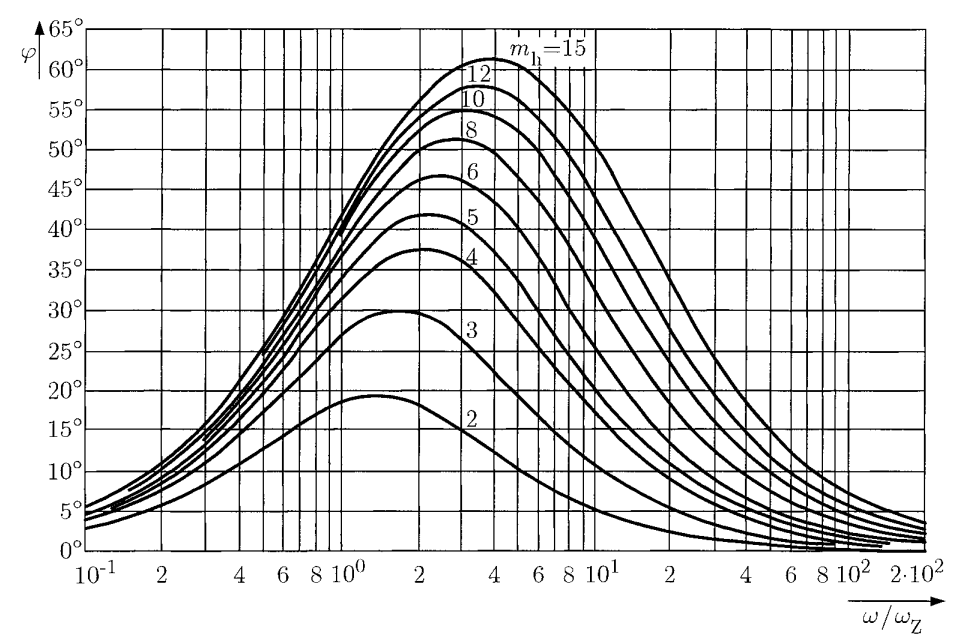
\includegraphics[width=0.8\textwidth]{Abbildungen/Lead-Glied.png}
    
    % Hier kommt deine Bildunterschrift hin
    \caption{Lead-Glied Dimensionierung.}
    
    % Der Label-Name, um im Text mit \ref{fig:mein_bild} darauf zu verweisen
    \label{fig:Lead-Glied}
\end{figure}

\noindent Die Phase muss um circa 50° gehoben werden, weshalb $m_{\mathrm{h}} = 8$ verwendet wird. Für die Grenzen gilt:
$$\omega_{\mathrm{N}} = m_{\mathrm{h}} \cdot \omega_{\mathrm{Z}}$$
Durch Ablesen an der gwünschten Stelle im Diagramm ergibt sich für $\frac{\omega_{\mathrm{c}}}{\omega_{\mathrm{Z}}} = 2.7$. Außerdem werden noch diese Formeln benötigt für die Berechnung des Lead-Glieds:
\begin{equation}
\begin{aligned}
    G(s) &= \frac{1 + Ts}{1 + \alpha Ts} \\[1.5ex]
    \omega_{\mathrm{Z}} &= \frac{1}{T} \\[1.5ex]
    \omega_{\mathrm{N}} &= \frac{1}{\alpha T}
    \label{eq:lead_formeln}
\end{aligned}
\end{equation}

\begin{lstlisting}
wz = wc / 2.7;
wn = 8*wz;
T = 1/wz; % Umformen wz formel
alpha = 1 / (wn * T) % Umformen wn formel
G = tf([T 1], [alpha*T 1])
Gr = Gr * G;
G0 = Gs * Gr;
bode(G0); grid on;
\end{lstlisting}

\begin{figure}[H]
    \centering
    % Hier definierst du die Wunschgröße der Grafik:
    \setlength\figureheight{6cm}
    \setlength\figurewidth{0.8\textwidth} % 80% der Textbreite
    
    % Hier wird die TikZ-Datei geladen:
    % This file was created by matlab2tikz.
%
%The latest updates can be retrieved from
%  http://www.mathworks.com/matlabcentral/fileexchange/22022-matlab2tikz-matlab2tikz
%where you can also make suggestions and rate matlab2tikz.
%
\definecolor{mycolor1}{rgb}{0.49020,0.49020,0.49020}%
\definecolor{mycolor2}{rgb}{0.06600,0.44300,0.74500}%
\definecolor{mycolor3}{rgb}{0.12941,0.12941,0.12941}%
%
\begin{tikzpicture}

\begin{axis}[%
width=4.863in,
height=1.271in,
at={(0.837in,1.891in)},
scale only axis,
unbounded coords=jump,
xmode=log,
xmin=0.01,
title={Bode-Diagramm},
xmax=100,
xtick={0.01,0.1,1,10,100},
xticklabels={\empty},
xminorticks=true,
ymin=-60,
ymax=80,
ylabel style={font=\color{mycolor3}},
ylabel={Magnitude (dB)},
axis background/.style={fill=white},
xmajorgrids,
ymajorgrids
]
\addplot [color=mycolor1, line width=1.5pt, forget plot]
  table[row sep=crcr]{%
nan	-60\\
nan	80\\
};
\addplot [color=mycolor1, line width=1.5pt, forget plot]
  table[row sep=crcr]{%
nan	-60\\
nan	80\\
};
\addplot [color=mycolor2, forget plot]
  table[row sep=crcr]{%
-100	-42.5133608629331\\
-94.0057378228297	-41.4438240404289\\
-88.370787436146	-40.3748462475963\\
-83.0736107491936	-39.3064995674997\\
-78.093960720845	-38.2388651600445\\
-73.4128039707012	-37.1720343448039\\
-69.0122480290853	-36.1061097963698\\
-64.8754729478629	-35.0412068592143\\
-60.9866670106888	-33.9774549880213\\
-57.3309662969503	-32.9149993178471\\
-53.894397868406	-31.8540023661312\\
-50.6638263613665	-30.7946458653286\\
-47.6269037802799	-29.7371327205445\\
-44.7720223008213	-28.6816890808028\\
-42.0882699020889	-27.6285665051983\\
-39.5653886583227	-26.5780441959255\\
-37.1937355307264	-25.5304312587845\\
-34.9642455095314	-24.4860689380539\\
-32.8683969654206	-23.4453327564768\\
-30.8981790778802	-22.4086344725781\\
-29.0460612159805	-21.3764237468968\\
-27.3049641545532	-20.3491893865613\\
-25.6682330157469	-19.3274600149798\\
-24.1296118325361	-18.3118039917923\\
-22.6832196369604	-17.3028283897844\\
-21.3235279816976	-16.3011768229815\\
-20.0453398090524	-15.307525917037\\
-18.8437695865931	-14.3225802231414\\
-17.7142246335108	-13.3470654040077\\
-16.6523875663253	-12.3817195686279\\
-15.6541997968413	-11.427282703967\\
-14.7158460192806	-10.4844842471466\\
-13.8337396272962	-9.5540289587208\\
-13.004509005129	-8.63658139054333\\
-12.2249846405078	-7.73274938072374\\
-11.492187010037	-6.8430671398591\\
-10.8033151907647	-5.96797860116587\\
-10.1557361544042	-5.10782177579583\\
-9.54697470328752	-4.26281486908403\\
-8.97470400958434	-3.43304486434072\\
-8.43673672162485	-2.61845916620736\\
-7.93101660333306	-1.81886072269515\\
-7.45561067481437	-1.03390682980424\\
-7.0087018240569	-0.263111587986891\\
-6.58858186150681	0.494148247936429\\
-6.19364499097061	1.23862447877882\\
-5.82238167188866	1.97118632560685\\
-5.47337284952014	2.69280761805724\\
-5.14528453098585	3.40455297855239\\
-4.83686268643717	4.10756361074396\\
-4.54692845586241	4.80304318061282\\
-4.27437364320966	5.49224411775213\\
-4.01815648060381	6.17645447879681\\
-3.77729764646746	6.8569853201495\\
-3.55087652232611	7.53515833620327\\
-3.3380276739903	8.21229334260324\\
-3.13793754366482	8.88969502997943\\
-2.9498413403417	9.56863828930982\\
-2.77302011659106	10.2503513235932\\
-2.60679802057692	10.9359957222876\\
-2.45053971279426	11.6266426997478\\
-2.30364793765369	12.3232448072131\\
-2.16556124063176	13.0266026469113\\
-2.03575182226111	13.7373264800291\\
-1.91372352075826	14.4557931650241\\
-1.79900991557783	15.1820996245003\\
-1.69117254464481	15.9160150402781\\
-1.58979922845048	16.6569352089133\\
-1.49450249460652	17.4038438875411\\
-1.40491809683546	18.1552873645696\\
-1.32070362273663	18.9093696179577\\
-1.24153718500641	19.6637758503177\\
-1.16711619111007	20.4158313785315\\
-1.09715618670273	21.1626002722767\\
-1.03138976837872	21.9010234689247\\
-0.969565561593592	22.6280895486495\\
-0.911447259852119	23.3410239198667\\
-0.856812721489948	24.0374756362762\\
-0.805453120596493	24.7156776558111\\
-0.75717214883374	25.374557872043\\
-0.711785265100132	26.0137851728978\\
-0.669118990171564	26.6337457173811\\
-0.629010243623446	27.2354566376545\\
-0.591305720499399	27.8204341344209\\
-0.55586130534406	28.3905380458237\\
-0.522541521360296	28.9478148149598\\
-0.491219012585385	29.4943564460079\\
-0.46177405710691	30.0321865520422\\
-0.434094109457766	30.5631779951768\\
-0.408073370441215	31.089001308357\\
-0.383612382741754	31.6110996598334\\
-0.360617650776123	32.1306845116547\\
-0.33900128333145	32.6487459051122\\
-0.318680657624591	33.1660719538166\\
-0.299578103498643	33.6832731811397\\
-0.28162060654954	34.200808478951\\
-0.264739529048023	34.7190104990534\\
-0.248870347590279	35.2381091319515\\
-0.233952406474482	35.7582523618999\\
-0.219928685860603	36.2795242319832\\
-0.206745583827313	36.8019599432254\\
-0.194352711492983	37.3255582850272\\
-0.182702700417654	37.8502916843137\\
-0.17175102154985	38.3761141949434\\
-0.161455815026184	38.9029677478402\\
-0.151777730173227	39.4307869607404\\
-0.142679775100086	39.9595027744957\\
-0.13412717530679	40.4890451470863\\
-0.126087240768068	41.0193450009047\\
-0.11852924098447	41.5503355857446\\
-0.111424287523251	42.0819533903855\\
-0.104745223600063	42.6141387101077\\
-0.0984665202794124	43.1468359558395\\
-0.0925641788971278	43.6799937726535\\
-0.0870156393318891	44.2135650205813\\
-0.0817996937751947	44.7475066587634\\
-0.0768964056701872	45.2817795643639\\
-0.0722870335094957	45.8163483100591\\
-0.0679539592008376	46.3511809179019\\
-0.0638806207265721	46.8862486026667\\
-0.0600514488398176	47.4215255141386\\
-0.0564518075551697	47.9569884850065\\
-0.0530679382065612	48.4926167888873\\
-0.0498869068584412	49.0283919113958\\
-0.0468965548692655	49.5642973359733\\
-0.0440854524183412	50.1003183453052\\
-0.0414428548183942	50.6364418385199\\
-0.0389586614468756	51.1726561639105\\
-0.0366233771390337	51.7089509666127\\
-0.0344280758951862	52.2453170504737\\
-0.0323643667634736	52.7817462532251\\
-0.03042436176769	53.3182313340107\\
-0.0286006457576039	53.8547658723032\\
-0.0268862480665294	54.3913441772522\\
-0.0252746158678173	54.927961206539\\
-0.0237595891284276	55.4646124938577\\
-0.0223353770638512	56.001294084197\\
-0.0209965360043844	56.5380024761516\\
-0.0197379485881577	57.0747345705567\\
-0.0185548042013884	57.6114876247926\\
-0.0174425805910966	58.1482592121659\\
-0.0163970265800021	58.685047185831\\
-0.0154141458175364	59.221849646762\\
-0.014490181504862	59.7586649153357\\
-0.0136216020355127	60.2954915061324\\
-0.0128050874967733	60.8323281055974\\
-0.0120375169802007	61.3691735522462\\
-0.0113159566527861	61.9060268191308\\
-0.0106376485431631	62.4428869983105\\
-0.01	62.9797532871047\\
0.01	62.9797532871047\\
0.0106376485431631	62.4428869983105\\
0.0113159566527861	61.9060268191308\\
0.0120375169802007	61.3691735522462\\
0.0128050874967733	60.8323281055974\\
0.0136216020355127	60.2954915061324\\
0.014490181504862	59.7586649153357\\
0.0154141458175364	59.221849646762\\
0.0163970265800021	58.685047185831\\
0.0174425805910966	58.1482592121659\\
0.0185548042013884	57.6114876247926\\
0.0197379485881577	57.0747345705567\\
0.0209965360043844	56.5380024761516\\
0.0223353770638512	56.001294084197\\
0.0237595891284276	55.4646124938577\\
0.0252746158678173	54.927961206539\\
0.0268862480665294	54.3913441772522\\
0.0286006457576039	53.8547658723032\\
0.03042436176769	53.3182313340107\\
0.0323643667634736	52.7817462532251\\
0.0344280758951862	52.2453170504737\\
0.0366233771390337	51.7089509666127\\
0.0389586614468756	51.1726561639105\\
0.0414428548183942	50.6364418385199\\
0.0440854524183412	50.1003183453052\\
0.0468965548692655	49.5642973359733\\
0.0498869068584412	49.0283919113958\\
0.0530679382065612	48.4926167888873\\
0.0564518075551697	47.9569884850065\\
0.0600514488398176	47.4215255141386\\
0.0638806207265721	46.8862486026667\\
0.0679539592008376	46.3511809179019\\
0.0722870335094957	45.8163483100591\\
0.0768964056701872	45.2817795643639\\
0.0817996937751947	44.7475066587634\\
0.0870156393318891	44.2135650205813\\
0.0925641788971278	43.6799937726535\\
0.0984665202794124	43.1468359558395\\
0.104745223600063	42.6141387101077\\
0.111424287523251	42.0819533903855\\
0.11852924098447	41.5503355857446\\
0.126087240768068	41.0193450009047\\
0.13412717530679	40.4890451470863\\
0.142679775100086	39.9595027744957\\
0.151777730173227	39.4307869607404\\
0.161455815026184	38.9029677478402\\
0.17175102154985	38.3761141949434\\
0.182702700417654	37.8502916843137\\
0.194352711492983	37.3255582850272\\
0.206745583827313	36.8019599432254\\
0.219928685860603	36.2795242319832\\
0.233952406474482	35.7582523618999\\
0.248870347590279	35.2381091319515\\
0.264739529048023	34.7190104990534\\
0.28162060654954	34.200808478951\\
0.299578103498643	33.6832731811397\\
0.318680657624591	33.1660719538166\\
0.33900128333145	32.6487459051122\\
0.360617650776123	32.1306845116547\\
0.383612382741754	31.6110996598334\\
0.408073370441215	31.089001308357\\
0.434094109457766	30.5631779951768\\
0.46177405710691	30.0321865520422\\
0.491219012585385	29.4943564460079\\
0.522541521360296	28.9478148149598\\
0.55586130534406	28.3905380458237\\
0.591305720499399	27.8204341344209\\
0.629010243623446	27.2354566376545\\
0.669118990171564	26.6337457173811\\
0.711785265100132	26.0137851728978\\
0.75717214883374	25.374557872043\\
0.805453120596493	24.7156776558111\\
0.856812721489948	24.0374756362762\\
0.911447259852119	23.3410239198667\\
0.969565561593592	22.6280895486495\\
1.03138976837872	21.9010234689247\\
1.09715618670273	21.1626002722767\\
1.16711619111007	20.4158313785315\\
1.24153718500641	19.6637758503177\\
1.32070362273663	18.9093696179577\\
1.40491809683546	18.1552873645696\\
1.49450249460652	17.4038438875411\\
1.58979922845048	16.6569352089133\\
1.69117254464481	15.9160150402781\\
1.79900991557783	15.1820996245003\\
1.91372352075826	14.4557931650241\\
2.03575182226111	13.7373264800291\\
2.16556124063176	13.0266026469113\\
2.30364793765369	12.3232448072131\\
2.45053971279426	11.6266426997478\\
2.60679802057692	10.9359957222876\\
2.77302011659106	10.2503513235932\\
2.9498413403417	9.56863828930982\\
3.13793754366482	8.88969502997943\\
3.3380276739903	8.21229334260324\\
3.55087652232611	7.53515833620327\\
3.77729764646746	6.8569853201495\\
4.01815648060381	6.17645447879681\\
4.27437364320966	5.49224411775213\\
4.54692845586241	4.80304318061282\\
4.83686268643717	4.10756361074396\\
5.14528453098585	3.40455297855239\\
5.47337284952014	2.69280761805724\\
5.82238167188866	1.97118632560685\\
6.19364499097061	1.23862447877882\\
6.58858186150681	0.494148247936429\\
7.0087018240569	-0.263111587986891\\
7.45561067481437	-1.03390682980424\\
7.93101660333306	-1.81886072269515\\
8.43673672162485	-2.61845916620736\\
8.97470400958434	-3.43304486434072\\
9.54697470328752	-4.26281486908403\\
10.1557361544042	-5.10782177579583\\
10.8033151907647	-5.96797860116587\\
11.492187010037	-6.8430671398591\\
12.2249846405078	-7.73274938072374\\
13.004509005129	-8.63658139054333\\
13.8337396272962	-9.5540289587208\\
14.7158460192806	-10.4844842471466\\
15.6541997968413	-11.427282703967\\
16.6523875663253	-12.3817195686279\\
17.7142246335108	-13.3470654040077\\
18.8437695865931	-14.3225802231414\\
20.0453398090524	-15.307525917037\\
21.3235279816976	-16.3011768229815\\
22.6832196369604	-17.3028283897844\\
24.1296118325361	-18.3118039917923\\
25.6682330157469	-19.3274600149798\\
27.3049641545532	-20.3491893865613\\
29.0460612159805	-21.3764237468968\\
30.8981790778802	-22.4086344725781\\
32.8683969654206	-23.4453327564768\\
34.9642455095314	-24.4860689380539\\
37.1937355307264	-25.5304312587845\\
39.5653886583227	-26.5780441959255\\
42.0882699020889	-27.6285665051983\\
44.7720223008213	-28.6816890808028\\
47.6269037802799	-29.7371327205445\\
50.6638263613665	-30.7946458653286\\
53.894397868406	-31.8540023661312\\
57.3309662969503	-32.9149993178471\\
60.9866670106888	-33.9774549880213\\
64.8754729478629	-35.0412068592143\\
69.0122480290853	-36.1061097963698\\
73.4128039707012	-37.1720343448039\\
78.093960720845	-38.2388651600445\\
83.0736107491936	-39.3064995674997\\
88.370787436146	-40.3748462475963\\
94.0057378228297	-41.4438240404289\\
100	-42.5133608629331\\
};
\end{axis}

\begin{axis}[%
width=4.863in,
height=1.271in,
at={(0.837in,0.317in)},
scale only axis,
unbounded coords=jump,
xmode=log,
xmin=0.01,
xmax=100,
xminorticks=true,
ymin=-180,
ymax=-90,
ytick={-180, -150, -120,  -90},
ylabel style={font=\color{mycolor3}},
ylabel={Phase (deg)},
xlabel={Frequenz (rad/s)},
axis background/.style={fill=white},
xmajorgrids,
ymajorgrids
]
\addplot [color=mycolor1, line width=1.5pt, forget plot]
  table[row sep=crcr]{%
nan	-180\\
nan	-90\\
};
\addplot [color=mycolor1, line width=1.5pt, forget plot]
  table[row sep=crcr]{%
nan	-180\\
nan	-90\\
};
\addplot [color=mycolor2, forget plot]
  table[row sep=crcr]{%
-100	175.410143887306\\
-94.0057378228297	175.119269421921\\
-88.370787436146	174.810210733685\\
-83.0736107491936	174.481881333953\\
-78.093960720845	174.133139973908\\
-73.4128039707012	173.762789983682\\
-69.0122480290853	173.369579101372\\
-64.8754729478629	172.952199916145\\
-60.9866670106888	172.509291071256\\
-57.3309662969503	172.039439396957\\
-53.894397868406	171.541183169758\\
-50.6638263613665	171.013016723062\\
-47.6269037802799	170.45339666415\\
-44.7720223008213	169.860749982914\\
-42.0882699020889	169.233484367101\\
-39.5653886583227	168.570001065038\\
-37.1937355307264	167.868710656997\\
-34.9642455095314	167.128052106695\\
-32.8683969654206	166.346515460128\\
-30.8981790778802	165.522668534048\\
-29.0460612159805	164.655187883986\\
-27.3049641545532	163.742894254003\\
-25.6682330157469	162.78479257902\\
-24.1296118325361	161.780116427869\\
-22.6832196369604	160.728376534706\\
-21.3235279816976	159.629412764763\\
-20.0453398090524	158.483448499409\\
-18.8437695865931	157.291146014167\\
-17.7142246335108	156.053660980203\\
-16.6523875663253	154.77269377504\\
-15.6541997968413	153.45053488374\\
-14.7158460192806	152.090101360582\\
-13.8337396272962	150.694961163508\\
-13.004509005129	149.269342229734\\
-12.2249846405078	147.818123482337\\
-11.492187010037	146.346805574569\\
-10.8033151907647	144.861460089324\\
-10.1557361544042	143.368657072342\\
-9.54697470328752	141.875372102312\\
-8.97470400958434	140.388875463126\\
-8.43673672162485	138.916607232872\\
-7.93101660333306	137.466043088177\\
-7.45561067481437	136.04455621146\\
-7.0087018240569	134.659280799702\\
-6.58858186150681	133.316982285974\\
-6.19364499097061	132.02393854577\\
-5.82238167188866	130.785835174049\\
-5.47337284952014	129.607676530431\\
-5.14528453098585	128.493712818903\\
-4.83686268643717	127.447382145387\\
-4.54692845586241	126.471265404268\\
-4.27437364320966	125.567051067902\\
-4.01815648060381	124.735506535804\\
-3.77729764646746	123.976452653499\\
-3.55087652232611	123.288738322906\\
-3.3380276739903	122.67021277333\\
-3.13793754366482	122.1176940214\\
-2.9498413403417	121.626933303006\\
-2.77302011659106	121.192576803333\\
-2.60679802057692	120.80812784187\\
-2.45053971279426	120.465914784599\\
-2.30364793765369	120.157072334134\\
-2.16556124063176	119.871546427469\\
-2.03575182226111	119.598135613923\\
-1.91372352075826	119.324584242005\\
-1.79900991557783	119.037744640438\\
-1.69117254464481	118.723826113377\\
-1.58979922845048	118.368747122442\\
-1.49450249460652	117.958602421564\\
-1.40491809683546	117.480247976415\\
-1.32070362273663	116.921992274077\\
-1.24153718500641	116.274362871406\\
-1.16711619111007	115.53089296042\\
-1.09715618670273	114.688847789801\\
-1.03138976837872	113.749791032358\\
-0.969565561593592	112.719884694121\\
-0.911447259852119	111.609830844112\\
-0.856812721489948	110.434403485921\\
-0.805453120596493	109.211580941053\\
-0.75717214883374	107.961360608153\\
-0.711785265100132	106.704399702552\\
-0.669118990171564	105.460658600162\\
-0.629010243623446	104.248217157222\\
-0.591305720499399	103.082391605529\\
-0.55586130534406	101.975214972788\\
-0.522541521360296	100.93527716903\\
-0.491219012585385	99.9678686207862\\
-0.46177405710691	99.0753421699849\\
-0.434094109457766	98.2576017190086\\
-0.408073370441215	97.5126367969413\\
-0.383612382741754	96.8370418902718\\
-0.360617650776123	96.2264810859695\\
-0.33900128333145	95.6760777669333\\
-0.318680657624591	95.1807236691421\\
-0.299578103498643	94.7353112448316\\
-0.28162060654954	94.3348986786447\\
-0.264739529048023	93.9748191581136\\
-0.248870347590279	93.6507461799916\\
-0.233952406474482	93.3587256580279\\
-0.219928685860603	93.0951840190256\\
-0.206745583827313	92.8569197433767\\
-0.194352711492983	92.6410841621944\\
-0.182702700417654	92.4451558838533\\
-0.17175102154985	92.2669120298255\\
-0.161455815026184	92.1043985104102\\
-0.151777730173227	91.9559008400215\\
-0.142679775100086	91.8199164448602\\
-0.13412717530679	91.6951290177238\\
-0.126087240768068	91.5803851930028\\
-0.11852924098447	91.4746736218453\\
-0.111424287523251	91.3771064003544\\
-0.104745223600063	91.2869027245665\\
-0.0984665202794124	91.2033746009782\\
-0.0925641788971278	91.1259144200987\\
-0.0870156393318891	91.0539841951445\\
-0.0817996937751947	90.9871062729418\\
-0.0768964056701872	90.9248553353227\\
-0.0722870335094957	90.8668515239992\\
-0.0679539592008376	90.8127545381288\\
-0.0638806207265721	90.7622585702983\\
-0.0600514488398176	90.7150879626239\\
-0.0564518075551697	90.6709934796133\\
-0.0530679382065612	90.6297491081168\\
-0.0498869068584412	90.5911493069881\\
-0.0468965548692655	90.5550066399839\\
-0.0440854524183412	90.5211497350184\\
-0.0414428548183942	90.4894215212303\\
-0.0389586614468756	90.4596777025447\\
-0.0366233771390337	90.431785432626\\
-0.0344280758951862	90.4056221614446\\
-0.0323643667634736	90.3810746282223\\
-0.03042436176769	90.358037979394\\
-0.0286006457576039	90.3364149935032\\
-0.0268862480665294	90.3161153977323\\
-0.0252746158678173	90.2970552631203\\
-0.0237595891284276	90.2791564675086\\
-0.0223353770638512	90.2623462169308\\
-0.0209965360043844	90.2465566175757\\
-0.0197379485881577	90.2317242916437\\
-0.0185548042013884	90.2177900314207\\
-0.0174425805910966	90.2046984867368\\
-0.0163970265800021	90.1923978816901\\
-0.0154141458175364	90.1808397571148\\
-0.014490181504862	90.1699787357797\\
-0.0136216020355127	90.1597723077286\\
-0.0128050874967733	90.150180633534\\
-0.0120375169802007	90.1411663635418\\
-0.0113159566527861	90.1326944714416\\
-0.0106376485431631	90.1247321007142\\
-0.01	90.1172484226974\\
0.01	-90.1172484226974\\
0.0106376485431631	-90.1247321007142\\
0.0113159566527861	-90.1326944714416\\
0.0120375169802007	-90.1411663635418\\
0.0128050874967733	-90.150180633534\\
0.0136216020355127	-90.1597723077286\\
0.014490181504862	-90.1699787357797\\
0.0154141458175364	-90.1808397571148\\
0.0163970265800021	-90.1923978816901\\
0.0174425805910966	-90.2046984867368\\
0.0185548042013884	-90.2177900314207\\
0.0197379485881577	-90.2317242916437\\
0.0209965360043844	-90.2465566175757\\
0.0223353770638512	-90.2623462169308\\
0.0237595891284276	-90.2791564675086\\
0.0252746158678173	-90.2970552631203\\
0.0268862480665294	-90.3161153977323\\
0.0286006457576039	-90.3364149935032\\
0.03042436176769	-90.358037979394\\
0.0323643667634736	-90.3810746282223\\
0.0344280758951862	-90.4056221614446\\
0.0366233771390337	-90.431785432626\\
0.0389586614468756	-90.4596777025447\\
0.0414428548183942	-90.4894215212303\\
0.0440854524183412	-90.5211497350184\\
0.0468965548692655	-90.5550066399839\\
0.0498869068584412	-90.5911493069881\\
0.0530679382065612	-90.6297491081168\\
0.0564518075551697	-90.6709934796133\\
0.0600514488398176	-90.7150879626239\\
0.0638806207265721	-90.7622585702983\\
0.0679539592008376	-90.8127545381288\\
0.0722870335094957	-90.8668515239992\\
0.0768964056701872	-90.9248553353227\\
0.0817996937751947	-90.9871062729418\\
0.0870156393318891	-91.0539841951445\\
0.0925641788971278	-91.1259144200987\\
0.0984665202794124	-91.2033746009782\\
0.104745223600063	-91.2869027245665\\
0.111424287523251	-91.3771064003544\\
0.11852924098447	-91.4746736218453\\
0.126087240768068	-91.5803851930028\\
0.13412717530679	-91.6951290177238\\
0.142679775100086	-91.8199164448602\\
0.151777730173227	-91.9559008400215\\
0.161455815026184	-92.1043985104102\\
0.17175102154985	-92.2669120298255\\
0.182702700417654	-92.4451558838533\\
0.194352711492983	-92.6410841621944\\
0.206745583827313	-92.8569197433767\\
0.219928685860603	-93.0951840190256\\
0.233952406474482	-93.3587256580279\\
0.248870347590279	-93.6507461799916\\
0.264739529048023	-93.9748191581136\\
0.28162060654954	-94.3348986786447\\
0.299578103498643	-94.7353112448316\\
0.318680657624591	-95.1807236691421\\
0.33900128333145	-95.6760777669333\\
0.360617650776123	-96.2264810859695\\
0.383612382741754	-96.8370418902718\\
0.408073370441215	-97.5126367969413\\
0.434094109457766	-98.2576017190086\\
0.46177405710691	-99.0753421699849\\
0.491219012585385	-99.9678686207862\\
0.522541521360296	-100.93527716903\\
0.55586130534406	-101.975214972788\\
0.591305720499399	-103.082391605529\\
0.629010243623446	-104.248217157222\\
0.669118990171564	-105.460658600162\\
0.711785265100132	-106.704399702552\\
0.75717214883374	-107.961360608153\\
0.805453120596493	-109.211580941053\\
0.856812721489948	-110.434403485921\\
0.911447259852119	-111.609830844112\\
0.969565561593592	-112.719884694121\\
1.03138976837872	-113.749791032358\\
1.09715618670273	-114.688847789801\\
1.16711619111007	-115.53089296042\\
1.24153718500641	-116.274362871406\\
1.32070362273663	-116.921992274077\\
1.40491809683546	-117.480247976415\\
1.49450249460652	-117.958602421564\\
1.58979922845048	-118.368747122442\\
1.69117254464481	-118.723826113377\\
1.79900991557783	-119.037744640438\\
1.91372352075826	-119.324584242005\\
2.03575182226111	-119.598135613923\\
2.16556124063176	-119.871546427469\\
2.30364793765369	-120.157072334134\\
2.45053971279426	-120.465914784599\\
2.60679802057692	-120.80812784187\\
2.77302011659106	-121.192576803333\\
2.9498413403417	-121.626933303006\\
3.13793754366482	-122.1176940214\\
3.3380276739903	-122.67021277333\\
3.55087652232611	-123.288738322906\\
3.77729764646746	-123.976452653499\\
4.01815648060381	-124.735506535804\\
4.27437364320966	-125.567051067902\\
4.54692845586241	-126.471265404268\\
4.83686268643717	-127.447382145387\\
5.14528453098585	-128.493712818903\\
5.47337284952014	-129.607676530431\\
5.82238167188866	-130.785835174049\\
6.19364499097061	-132.02393854577\\
6.58858186150681	-133.316982285974\\
7.0087018240569	-134.659280799702\\
7.45561067481437	-136.04455621146\\
7.93101660333306	-137.466043088177\\
8.43673672162485	-138.916607232872\\
8.97470400958434	-140.388875463126\\
9.54697470328752	-141.875372102312\\
10.1557361544042	-143.368657072342\\
10.8033151907647	-144.861460089324\\
11.492187010037	-146.346805574569\\
12.2249846405078	-147.818123482337\\
13.004509005129	-149.269342229734\\
13.8337396272962	-150.694961163508\\
14.7158460192806	-152.090101360582\\
15.6541997968413	-153.45053488374\\
16.6523875663253	-154.77269377504\\
17.7142246335108	-156.053660980203\\
18.8437695865931	-157.291146014167\\
20.0453398090524	-158.483448499409\\
21.3235279816976	-159.629412764763\\
22.6832196369604	-160.728376534706\\
24.1296118325361	-161.780116427869\\
25.6682330157469	-162.78479257902\\
27.3049641545532	-163.742894254003\\
29.0460612159805	-164.655187883986\\
30.8981790778802	-165.522668534048\\
32.8683969654206	-166.346515460128\\
34.9642455095314	-167.128052106695\\
37.1937355307264	-167.868710656997\\
39.5653886583227	-168.570001065038\\
42.0882699020889	-169.233484367101\\
44.7720223008213	-169.860749982914\\
47.6269037802799	-170.45339666415\\
50.6638263613665	-171.013016723062\\
53.894397868406	-171.541183169758\\
57.3309662969503	-172.039439396957\\
60.9866670106888	-172.509291071256\\
64.8754729478629	-172.952199916145\\
69.0122480290853	-173.369579101372\\
73.4128039707012	-173.762789983682\\
78.093960720845	-174.133139973908\\
83.0736107491936	-174.481881333953\\
88.370787436146	-174.810210733685\\
94.0057378228297	-175.119269421921\\
100	-175.410143887306\\
};
\addplot [color=mycolor1, line width=1.5pt, forget plot]
  table[row sep=crcr]{%
nan	-60\\
nan	80\\
};
\addplot [color=mycolor1, line width=1.5pt, forget plot]
  table[row sep=crcr]{%
nan	-60\\
nan	80\\
};
\end{axis}

\begin{axis}[%
width=5.833in,
height=3.511in,
at={(0in,0in)},
scale only axis,
xmin=0,
xmax=1,
ymin=0,
ymax=1,
axis line style={draw=none},
ticks=none,
axis x line*=bottom,
axis y line*=left
]
\end{axis}
\end{tikzpicture}%
    
    \caption{Sprungantwort der Phasenkorrigierten Strecke ($G_{\mathrm{0}}(s)$).}
    \label{fig:matlab_plot11}
\end{figure}

\noindent An der Frequenz 3rad/s ist die Phasenreserve jetzt bei circa 60°, was den Anforderungen entspricht. Allerdings hat sich durch die Phasenkorrektur die Durchtrittsfrequenz verschoben. Die Verstärkung muss um 8.5dB gesenkt werden.

\begin{lstlisting}
k = db2mag(-8.5)
Gr = Gr * k;
G0 = Gr * Gs;
bode(G0); grid on
step(G0/(1+G0)); grid on
\end{lstlisting}

\begin{figure}[H]
    \centering
    % Hier definierst du die Wunschgröße der Grafik:
    \setlength\figureheight{6cm}
    \setlength\figurewidth{0.8\textwidth} % 80% der Textbreite
    
    % Hier wird die TikZ-Datei geladen:
    % This file was created by matlab2tikz.
%
%The latest updates can be retrieved from
%  http://www.mathworks.com/matlabcentral/fileexchange/22022-matlab2tikz-matlab2tikz
%where you can also make suggestions and rate matlab2tikz.
%
\definecolor{mycolor1}{rgb}{0.49020,0.49020,0.49020}%
\definecolor{mycolor2}{rgb}{0.06600,0.44300,0.74500}%
\definecolor{mycolor3}{rgb}{0.12941,0.12941,0.12941}%
%
\begin{tikzpicture}

\begin{axis}[%
width=4.863in,
height=1.271in,
at={(0.837in,1.891in)},
scale only axis,
unbounded coords=jump,
xmode=log,
xmin=0.01,
title={Bode-Diagramm},
xmax=100,
xtick={0.01,0.1,1,10,100},
xticklabels={\empty},
xminorticks=true,
ymin=-60,
ymax=60,
ylabel style={font=\color{mycolor3}},
ylabel={Magnitude (dB)},
axis background/.style={fill=white},
xmajorgrids,
ymajorgrids
]
\addplot [color=mycolor1, line width=1.5pt, forget plot]
  table[row sep=crcr]{%
nan	-60\\
nan	60\\
};
\addplot [color=mycolor1, line width=1.5pt, forget plot]
  table[row sep=crcr]{%
nan	-60\\
nan	60\\
};
\addplot [color=mycolor2, forget plot]
  table[row sep=crcr]{%
-100	-51.0133608629331\\
-94.0057378228297	-49.9438240404289\\
-88.370787436146	-48.8748462475963\\
-83.0736107491936	-47.8064995674996\\
-78.093960720845	-46.7388651600445\\
-73.4128039707012	-45.6720343448039\\
-69.0122480290853	-44.6061097963698\\
-64.8754729478629	-43.5412068592143\\
-60.9866670106888	-42.4774549880213\\
-57.3309662969503	-41.4149993178471\\
-53.894397868406	-40.3540023661312\\
-50.6638263613665	-39.2946458653286\\
-47.6269037802799	-38.2371327205445\\
-44.7720223008213	-37.1816890808028\\
-42.0882699020889	-36.1285665051983\\
-39.5653886583227	-35.0780441959255\\
-37.1937355307264	-34.0304312587845\\
-34.9642455095314	-32.9860689380539\\
-32.8683969654206	-31.9453327564768\\
-30.8981790778802	-30.9086344725781\\
-29.0460612159805	-29.8764237468968\\
-27.3049641545532	-28.8491893865613\\
-25.6682330157469	-27.8274600149798\\
-24.1296118325361	-26.8118039917923\\
-22.6832196369604	-25.8028283897844\\
-21.3235279816976	-24.8011768229815\\
-20.0453398090524	-23.807525917037\\
-18.8437695865931	-22.8225802231414\\
-17.7142246335108	-21.8470654040077\\
-16.6523875663253	-20.8817195686279\\
-15.6541997968413	-19.927282703967\\
-14.7158460192806	-18.9844842471466\\
-13.8337396272962	-18.0540289587208\\
-13.004509005129	-17.1365813905433\\
-12.2249846405078	-16.2327493807237\\
-11.492187010037	-15.3430671398591\\
-10.8033151907647	-14.4679786011659\\
-10.1557361544042	-13.6078217757958\\
-9.54697470328752	-12.762814869084\\
-8.97470400958434	-11.9330448643407\\
-8.43673672162485	-11.1184591662074\\
-7.93101660333306	-10.3188607226952\\
-7.45561067481437	-9.53390682980424\\
-7.0087018240569	-8.76311158798689\\
-6.58858186150681	-8.00585175206357\\
-6.19364499097061	-7.26137552122117\\
-5.82238167188866	-6.52881367439314\\
-5.47337284952014	-5.80719238194276\\
-5.14528453098585	-5.09544702144761\\
-4.83686268643717	-4.39243638925604\\
-4.54692845586241	-3.69695681938718\\
-4.27437364320966	-3.00775588224787\\
-4.01815648060381	-2.32354552120319\\
-3.77729764646746	-1.6430146798505\\
-3.55087652232611	-0.964841663796727\\
-3.3380276739903	-0.287706657396758\\
-3.13793754366482	0.389695029979435\\
-2.9498413403417	1.06863828930982\\
-2.77302011659106	1.75035132359325\\
-2.60679802057692	2.43599572228759\\
-2.45053971279426	3.12664269974777\\
-2.30364793765369	3.82324480721312\\
-2.16556124063176	4.52660264691129\\
-2.03575182226111	5.23732648002911\\
-1.91372352075826	5.95579316502408\\
-1.79900991557783	6.68209962450033\\
-1.69117254464481	7.41601504027812\\
-1.58979922845048	8.15693520891332\\
-1.49450249460652	8.90384388754114\\
-1.40491809683546	9.65528736456958\\
-1.32070362273663	10.4093696179577\\
-1.24153718500641	11.1637758503177\\
-1.16711619111007	11.9158313785315\\
-1.09715618670273	12.6626002722767\\
-1.03138976837872	13.4010234689247\\
-0.969565561593592	14.1280895486495\\
-0.911447259852119	14.8410239198667\\
-0.856812721489948	15.5374756362762\\
-0.805453120596493	16.2156776558111\\
-0.75717214883374	16.874557872043\\
-0.711785265100132	17.5137851728978\\
-0.669118990171564	18.1337457173811\\
-0.629010243623446	18.7354566376545\\
-0.591305720499399	19.3204341344209\\
-0.55586130534406	19.8905380458237\\
-0.522541521360296	20.4478148149598\\
-0.491219012585385	20.9943564460079\\
-0.46177405710691	21.5321865520422\\
-0.434094109457766	22.0631779951768\\
-0.408073370441215	22.589001308357\\
-0.383612382741754	23.1110996598334\\
-0.360617650776123	23.6306845116547\\
-0.33900128333145	24.1487459051122\\
-0.318680657624591	24.6660719538166\\
-0.299578103498643	25.1832731811397\\
-0.28162060654954	25.700808478951\\
-0.264739529048023	26.2190104990534\\
-0.248870347590279	26.7381091319515\\
-0.233952406474482	27.2582523618999\\
-0.219928685860603	27.7795242319832\\
-0.206745583827313	28.3019599432254\\
-0.194352711492983	28.8255582850272\\
-0.182702700417654	29.3502916843137\\
-0.17175102154985	29.8761141949434\\
-0.161455815026184	30.4029677478402\\
-0.151777730173227	30.9307869607404\\
-0.142679775100086	31.4595027744957\\
-0.13412717530679	31.9890451470863\\
-0.126087240768068	32.5193450009047\\
-0.11852924098447	33.0503355857446\\
-0.111424287523251	33.5819533903854\\
-0.104745223600063	34.1141387101077\\
-0.0984665202794124	34.6468359558395\\
-0.0925641788971278	35.1799937726535\\
-0.0870156393318891	35.7135650205813\\
-0.0817996937751947	36.2475066587634\\
-0.0768964056701872	36.7817795643639\\
-0.0722870335094957	37.3163483100591\\
-0.0679539592008376	37.8511809179019\\
-0.0638806207265721	38.3862486026667\\
-0.0600514488398176	38.9215255141386\\
-0.0564518075551697	39.4569884850065\\
-0.0530679382065612	39.9926167888873\\
-0.0498869068584412	40.5283919113958\\
-0.0468965548692655	41.0642973359733\\
-0.0440854524183412	41.6003183453052\\
-0.0414428548183942	42.1364418385199\\
-0.0389586614468756	42.6726561639105\\
-0.0366233771390337	43.2089509666127\\
-0.0344280758951862	43.7453170504737\\
-0.0323643667634736	44.2817462532251\\
-0.03042436176769	44.8182313340107\\
-0.0286006457576039	45.3547658723032\\
-0.0268862480665294	45.8913441772522\\
-0.0252746158678173	46.4279612065389\\
-0.0237595891284276	46.9646124938577\\
-0.0223353770638512	47.501294084197\\
-0.0209965360043844	48.0380024761515\\
-0.0197379485881577	48.5747345705567\\
-0.0185548042013884	49.1114876247926\\
-0.0174425805910966	49.6482592121659\\
-0.0163970265800021	50.185047185831\\
-0.0154141458175364	50.721849646762\\
-0.014490181504862	51.2586649153357\\
-0.0136216020355127	51.7954915061324\\
-0.0128050874967733	52.3323281055973\\
-0.0120375169802007	52.8691735522462\\
-0.0113159566527861	53.4060268191308\\
-0.0106376485431631	53.9428869983105\\
-0.01	54.4797532871047\\
0.01	54.4797532871047\\
0.0106376485431631	53.9428869983105\\
0.0113159566527861	53.4060268191308\\
0.0120375169802007	52.8691735522462\\
0.0128050874967733	52.3323281055973\\
0.0136216020355127	51.7954915061324\\
0.014490181504862	51.2586649153357\\
0.0154141458175364	50.721849646762\\
0.0163970265800021	50.185047185831\\
0.0174425805910966	49.6482592121659\\
0.0185548042013884	49.1114876247926\\
0.0197379485881577	48.5747345705567\\
0.0209965360043844	48.0380024761515\\
0.0223353770638512	47.501294084197\\
0.0237595891284276	46.9646124938577\\
0.0252746158678173	46.4279612065389\\
0.0268862480665294	45.8913441772522\\
0.0286006457576039	45.3547658723032\\
0.03042436176769	44.8182313340107\\
0.0323643667634736	44.2817462532251\\
0.0344280758951862	43.7453170504737\\
0.0366233771390337	43.2089509666127\\
0.0389586614468756	42.6726561639105\\
0.0414428548183942	42.1364418385199\\
0.0440854524183412	41.6003183453052\\
0.0468965548692655	41.0642973359733\\
0.0498869068584412	40.5283919113958\\
0.0530679382065612	39.9926167888873\\
0.0564518075551697	39.4569884850065\\
0.0600514488398176	38.9215255141386\\
0.0638806207265721	38.3862486026667\\
0.0679539592008376	37.8511809179019\\
0.0722870335094957	37.3163483100591\\
0.0768964056701872	36.7817795643639\\
0.0817996937751947	36.2475066587634\\
0.0870156393318891	35.7135650205813\\
0.0925641788971278	35.1799937726535\\
0.0984665202794124	34.6468359558395\\
0.104745223600063	34.1141387101077\\
0.111424287523251	33.5819533903854\\
0.11852924098447	33.0503355857446\\
0.126087240768068	32.5193450009047\\
0.13412717530679	31.9890451470863\\
0.142679775100086	31.4595027744957\\
0.151777730173227	30.9307869607404\\
0.161455815026184	30.4029677478402\\
0.17175102154985	29.8761141949434\\
0.182702700417654	29.3502916843137\\
0.194352711492983	28.8255582850272\\
0.206745583827313	28.3019599432254\\
0.219928685860603	27.7795242319832\\
0.233952406474482	27.2582523618999\\
0.248870347590279	26.7381091319515\\
0.264739529048023	26.2190104990534\\
0.28162060654954	25.700808478951\\
0.299578103498643	25.1832731811397\\
0.318680657624591	24.6660719538166\\
0.33900128333145	24.1487459051122\\
0.360617650776123	23.6306845116547\\
0.383612382741754	23.1110996598334\\
0.408073370441215	22.589001308357\\
0.434094109457766	22.0631779951768\\
0.46177405710691	21.5321865520422\\
0.491219012585385	20.9943564460079\\
0.522541521360296	20.4478148149598\\
0.55586130534406	19.8905380458237\\
0.591305720499399	19.3204341344209\\
0.629010243623446	18.7354566376545\\
0.669118990171564	18.1337457173811\\
0.711785265100132	17.5137851728978\\
0.75717214883374	16.874557872043\\
0.805453120596493	16.2156776558111\\
0.856812721489948	15.5374756362762\\
0.911447259852119	14.8410239198667\\
0.969565561593592	14.1280895486495\\
1.03138976837872	13.4010234689247\\
1.09715618670273	12.6626002722767\\
1.16711619111007	11.9158313785315\\
1.24153718500641	11.1637758503177\\
1.32070362273663	10.4093696179577\\
1.40491809683546	9.65528736456958\\
1.49450249460652	8.90384388754114\\
1.58979922845048	8.15693520891332\\
1.69117254464481	7.41601504027812\\
1.79900991557783	6.68209962450033\\
1.91372352075826	5.95579316502408\\
2.03575182226111	5.23732648002911\\
2.16556124063176	4.52660264691129\\
2.30364793765369	3.82324480721312\\
2.45053971279426	3.12664269974777\\
2.60679802057692	2.43599572228759\\
2.77302011659106	1.75035132359325\\
2.9498413403417	1.06863828930982\\
3.13793754366482	0.389695029979435\\
3.3380276739903	-0.287706657396758\\
3.55087652232611	-0.964841663796727\\
3.77729764646746	-1.6430146798505\\
4.01815648060381	-2.32354552120319\\
4.27437364320966	-3.00775588224787\\
4.54692845586241	-3.69695681938718\\
4.83686268643717	-4.39243638925604\\
5.14528453098585	-5.09544702144761\\
5.47337284952014	-5.80719238194276\\
5.82238167188866	-6.52881367439314\\
6.19364499097061	-7.26137552122117\\
6.58858186150681	-8.00585175206357\\
7.0087018240569	-8.76311158798689\\
7.45561067481437	-9.53390682980424\\
7.93101660333306	-10.3188607226952\\
8.43673672162485	-11.1184591662074\\
8.97470400958434	-11.9330448643407\\
9.54697470328752	-12.762814869084\\
10.1557361544042	-13.6078217757958\\
10.8033151907647	-14.4679786011659\\
11.492187010037	-15.3430671398591\\
12.2249846405078	-16.2327493807237\\
13.004509005129	-17.1365813905433\\
13.8337396272962	-18.0540289587208\\
14.7158460192806	-18.9844842471466\\
15.6541997968413	-19.927282703967\\
16.6523875663253	-20.8817195686279\\
17.7142246335108	-21.8470654040077\\
18.8437695865931	-22.8225802231414\\
20.0453398090524	-23.807525917037\\
21.3235279816976	-24.8011768229815\\
22.6832196369604	-25.8028283897844\\
24.1296118325361	-26.8118039917923\\
25.6682330157469	-27.8274600149798\\
27.3049641545532	-28.8491893865613\\
29.0460612159805	-29.8764237468968\\
30.8981790778802	-30.9086344725781\\
32.8683969654206	-31.9453327564768\\
34.9642455095314	-32.9860689380539\\
37.1937355307264	-34.0304312587845\\
39.5653886583227	-35.0780441959255\\
42.0882699020889	-36.1285665051983\\
44.7720223008213	-37.1816890808028\\
47.6269037802799	-38.2371327205445\\
50.6638263613665	-39.2946458653286\\
53.894397868406	-40.3540023661312\\
57.3309662969503	-41.4149993178471\\
60.9866670106888	-42.4774549880213\\
64.8754729478629	-43.5412068592143\\
69.0122480290853	-44.6061097963698\\
73.4128039707012	-45.6720343448039\\
78.093960720845	-46.7388651600445\\
83.0736107491936	-47.8064995674996\\
88.370787436146	-48.8748462475963\\
94.0057378228297	-49.9438240404289\\
100	-51.0133608629331\\
};
\end{axis}

\begin{axis}[%
width=4.863in,
height=1.271in,
at={(0.837in,0.317in)},
scale only axis,
unbounded coords=jump,
xmode=log,
xmin=0.01,
xmax=100,
xminorticks=true,
ymin=-180,
ymax=-90,
ytick={-180, -150, -120,  -90},
ylabel style={font=\color{mycolor3}},
xlabel={Frequenz (rad/s)},
ylabel={Phase (deg)},
axis background/.style={fill=white},
xmajorgrids,
ymajorgrids
]
\addplot [color=mycolor1, line width=1.5pt, forget plot]
  table[row sep=crcr]{%
nan	-180\\
nan	-90\\
};
\addplot [color=mycolor1, line width=1.5pt, forget plot]
  table[row sep=crcr]{%
nan	-180\\
nan	-90\\
};
\addplot [color=mycolor2, forget plot]
  table[row sep=crcr]{%
-100	175.410143887306\\
-94.0057378228297	175.119269421921\\
-88.370787436146	174.810210733685\\
-83.0736107491936	174.481881333953\\
-78.093960720845	174.133139973908\\
-73.4128039707012	173.762789983682\\
-69.0122480290853	173.369579101372\\
-64.8754729478629	172.952199916145\\
-60.9866670106888	172.509291071256\\
-57.3309662969503	172.039439396957\\
-53.894397868406	171.541183169758\\
-50.6638263613665	171.013016723062\\
-47.6269037802799	170.45339666415\\
-44.7720223008213	169.860749982914\\
-42.0882699020889	169.233484367101\\
-39.5653886583227	168.570001065038\\
-37.1937355307264	167.868710656997\\
-34.9642455095314	167.128052106695\\
-32.8683969654206	166.346515460128\\
-30.8981790778802	165.522668534048\\
-29.0460612159805	164.655187883986\\
-27.3049641545532	163.742894254003\\
-25.6682330157469	162.78479257902\\
-24.1296118325361	161.780116427869\\
-22.6832196369604	160.728376534706\\
-21.3235279816976	159.629412764763\\
-20.0453398090524	158.483448499409\\
-18.8437695865931	157.291146014167\\
-17.7142246335108	156.053660980203\\
-16.6523875663253	154.77269377504\\
-15.6541997968413	153.45053488374\\
-14.7158460192806	152.090101360582\\
-13.8337396272962	150.694961163508\\
-13.004509005129	149.269342229734\\
-12.2249846405078	147.818123482337\\
-11.492187010037	146.346805574569\\
-10.8033151907647	144.861460089324\\
-10.1557361544042	143.368657072342\\
-9.54697470328752	141.875372102312\\
-8.97470400958434	140.388875463126\\
-8.43673672162485	138.916607232872\\
-7.93101660333306	137.466043088177\\
-7.45561067481437	136.04455621146\\
-7.0087018240569	134.659280799702\\
-6.58858186150681	133.316982285974\\
-6.19364499097061	132.02393854577\\
-5.82238167188866	130.785835174049\\
-5.47337284952014	129.607676530431\\
-5.14528453098585	128.493712818903\\
-4.83686268643717	127.447382145387\\
-4.54692845586241	126.471265404268\\
-4.27437364320966	125.567051067902\\
-4.01815648060381	124.735506535804\\
-3.77729764646746	123.976452653499\\
-3.55087652232611	123.288738322906\\
-3.3380276739903	122.67021277333\\
-3.13793754366482	122.1176940214\\
-2.9498413403417	121.626933303006\\
-2.77302011659106	121.192576803333\\
-2.60679802057692	120.80812784187\\
-2.45053971279426	120.465914784599\\
-2.30364793765369	120.157072334134\\
-2.16556124063176	119.871546427469\\
-2.03575182226111	119.598135613923\\
-1.91372352075826	119.324584242005\\
-1.79900991557783	119.037744640438\\
-1.69117254464481	118.723826113377\\
-1.58979922845048	118.368747122442\\
-1.49450249460652	117.958602421564\\
-1.40491809683546	117.480247976415\\
-1.32070362273663	116.921992274077\\
-1.24153718500641	116.274362871406\\
-1.16711619111007	115.530892960419\\
-1.09715618670273	114.688847789801\\
-1.03138976837872	113.749791032358\\
-0.969565561593592	112.719884694121\\
-0.911447259852119	111.609830844112\\
-0.856812721489948	110.434403485921\\
-0.805453120596493	109.211580941053\\
-0.75717214883374	107.961360608153\\
-0.711785265100132	106.704399702552\\
-0.669118990171564	105.460658600162\\
-0.629010243623446	104.248217157222\\
-0.591305720499399	103.082391605529\\
-0.55586130534406	101.975214972788\\
-0.522541521360296	100.93527716903\\
-0.491219012585385	99.9678686207862\\
-0.46177405710691	99.0753421699849\\
-0.434094109457766	98.2576017190086\\
-0.408073370441215	97.5126367969413\\
-0.383612382741754	96.8370418902718\\
-0.360617650776123	96.2264810859695\\
-0.33900128333145	95.6760777669333\\
-0.318680657624591	95.1807236691421\\
-0.299578103498643	94.7353112448316\\
-0.28162060654954	94.3348986786447\\
-0.264739529048023	93.9748191581136\\
-0.248870347590279	93.6507461799916\\
-0.233952406474482	93.3587256580279\\
-0.219928685860603	93.0951840190256\\
-0.206745583827313	92.8569197433767\\
-0.194352711492983	92.6410841621944\\
-0.182702700417654	92.4451558838533\\
-0.17175102154985	92.2669120298255\\
-0.161455815026184	92.1043985104102\\
-0.151777730173227	91.9559008400215\\
-0.142679775100086	91.8199164448602\\
-0.13412717530679	91.6951290177238\\
-0.126087240768068	91.5803851930028\\
-0.11852924098447	91.4746736218453\\
-0.111424287523251	91.3771064003544\\
-0.104745223600063	91.2869027245665\\
-0.0984665202794124	91.2033746009782\\
-0.0925641788971278	91.1259144200987\\
-0.0870156393318891	91.0539841951445\\
-0.0817996937751947	90.9871062729418\\
-0.0768964056701872	90.9248553353227\\
-0.0722870335094957	90.8668515239992\\
-0.0679539592008376	90.8127545381288\\
-0.0638806207265721	90.7622585702983\\
-0.0600514488398176	90.7150879626239\\
-0.0564518075551697	90.6709934796132\\
-0.0530679382065612	90.6297491081168\\
-0.0498869068584412	90.5911493069881\\
-0.0468965548692655	90.5550066399839\\
-0.0440854524183412	90.5211497350183\\
-0.0414428548183942	90.4894215212303\\
-0.0389586614468756	90.4596777025446\\
-0.0366233771390337	90.431785432626\\
-0.0344280758951862	90.4056221614446\\
-0.0323643667634736	90.3810746282223\\
-0.03042436176769	90.358037979394\\
-0.0286006457576039	90.3364149935032\\
-0.0268862480665294	90.3161153977323\\
-0.0252746158678173	90.2970552631203\\
-0.0237595891284276	90.2791564675086\\
-0.0223353770638512	90.2623462169308\\
-0.0209965360043844	90.2465566175757\\
-0.0197379485881577	90.2317242916437\\
-0.0185548042013884	90.2177900314207\\
-0.0174425805910966	90.2046984867368\\
-0.0163970265800021	90.1923978816901\\
-0.0154141458175364	90.1808397571148\\
-0.014490181504862	90.1699787357797\\
-0.0136216020355127	90.1597723077286\\
-0.0128050874967733	90.150180633534\\
-0.0120375169802007	90.1411663635418\\
-0.0113159566527861	90.1326944714416\\
-0.0106376485431631	90.1247321007142\\
-0.01	90.1172484226974\\
0.01	-90.1172484226974\\
0.0106376485431631	-90.1247321007142\\
0.0113159566527861	-90.1326944714416\\
0.0120375169802007	-90.1411663635418\\
0.0128050874967733	-90.150180633534\\
0.0136216020355127	-90.1597723077286\\
0.014490181504862	-90.1699787357797\\
0.0154141458175364	-90.1808397571148\\
0.0163970265800021	-90.1923978816901\\
0.0174425805910966	-90.2046984867368\\
0.0185548042013884	-90.2177900314207\\
0.0197379485881577	-90.2317242916437\\
0.0209965360043844	-90.2465566175757\\
0.0223353770638512	-90.2623462169308\\
0.0237595891284276	-90.2791564675086\\
0.0252746158678173	-90.2970552631203\\
0.0268862480665294	-90.3161153977323\\
0.0286006457576039	-90.3364149935032\\
0.03042436176769	-90.358037979394\\
0.0323643667634736	-90.3810746282223\\
0.0344280758951862	-90.4056221614446\\
0.0366233771390337	-90.431785432626\\
0.0389586614468756	-90.4596777025446\\
0.0414428548183942	-90.4894215212303\\
0.0440854524183412	-90.5211497350183\\
0.0468965548692655	-90.5550066399839\\
0.0498869068584412	-90.5911493069881\\
0.0530679382065612	-90.6297491081168\\
0.0564518075551697	-90.6709934796132\\
0.0600514488398176	-90.7150879626239\\
0.0638806207265721	-90.7622585702983\\
0.0679539592008376	-90.8127545381288\\
0.0722870335094957	-90.8668515239992\\
0.0768964056701872	-90.9248553353227\\
0.0817996937751947	-90.9871062729418\\
0.0870156393318891	-91.0539841951445\\
0.0925641788971278	-91.1259144200987\\
0.0984665202794124	-91.2033746009782\\
0.104745223600063	-91.2869027245665\\
0.111424287523251	-91.3771064003544\\
0.11852924098447	-91.4746736218453\\
0.126087240768068	-91.5803851930028\\
0.13412717530679	-91.6951290177238\\
0.142679775100086	-91.8199164448602\\
0.151777730173227	-91.9559008400215\\
0.161455815026184	-92.1043985104102\\
0.17175102154985	-92.2669120298255\\
0.182702700417654	-92.4451558838533\\
0.194352711492983	-92.6410841621944\\
0.206745583827313	-92.8569197433767\\
0.219928685860603	-93.0951840190256\\
0.233952406474482	-93.3587256580279\\
0.248870347590279	-93.6507461799916\\
0.264739529048023	-93.9748191581136\\
0.28162060654954	-94.3348986786447\\
0.299578103498643	-94.7353112448316\\
0.318680657624591	-95.1807236691421\\
0.33900128333145	-95.6760777669333\\
0.360617650776123	-96.2264810859695\\
0.383612382741754	-96.8370418902718\\
0.408073370441215	-97.5126367969413\\
0.434094109457766	-98.2576017190086\\
0.46177405710691	-99.0753421699849\\
0.491219012585385	-99.9678686207862\\
0.522541521360296	-100.93527716903\\
0.55586130534406	-101.975214972788\\
0.591305720499399	-103.082391605529\\
0.629010243623446	-104.248217157222\\
0.669118990171564	-105.460658600162\\
0.711785265100132	-106.704399702552\\
0.75717214883374	-107.961360608153\\
0.805453120596493	-109.211580941053\\
0.856812721489948	-110.434403485921\\
0.911447259852119	-111.609830844112\\
0.969565561593592	-112.719884694121\\
1.03138976837872	-113.749791032358\\
1.09715618670273	-114.688847789801\\
1.16711619111007	-115.530892960419\\
1.24153718500641	-116.274362871406\\
1.32070362273663	-116.921992274077\\
1.40491809683546	-117.480247976415\\
1.49450249460652	-117.958602421564\\
1.58979922845048	-118.368747122442\\
1.69117254464481	-118.723826113377\\
1.79900991557783	-119.037744640438\\
1.91372352075826	-119.324584242005\\
2.03575182226111	-119.598135613923\\
2.16556124063176	-119.871546427469\\
2.30364793765369	-120.157072334134\\
2.45053971279426	-120.465914784599\\
2.60679802057692	-120.80812784187\\
2.77302011659106	-121.192576803333\\
2.9498413403417	-121.626933303006\\
3.13793754366482	-122.1176940214\\
3.3380276739903	-122.67021277333\\
3.55087652232611	-123.288738322906\\
3.77729764646746	-123.976452653499\\
4.01815648060381	-124.735506535804\\
4.27437364320966	-125.567051067902\\
4.54692845586241	-126.471265404268\\
4.83686268643717	-127.447382145387\\
5.14528453098585	-128.493712818903\\
5.47337284952014	-129.607676530431\\
5.82238167188866	-130.785835174049\\
6.19364499097061	-132.02393854577\\
6.58858186150681	-133.316982285974\\
7.0087018240569	-134.659280799702\\
7.45561067481437	-136.04455621146\\
7.93101660333306	-137.466043088177\\
8.43673672162485	-138.916607232872\\
8.97470400958434	-140.388875463126\\
9.54697470328752	-141.875372102312\\
10.1557361544042	-143.368657072342\\
10.8033151907647	-144.861460089324\\
11.492187010037	-146.346805574569\\
12.2249846405078	-147.818123482337\\
13.004509005129	-149.269342229734\\
13.8337396272962	-150.694961163508\\
14.7158460192806	-152.090101360582\\
15.6541997968413	-153.45053488374\\
16.6523875663253	-154.77269377504\\
17.7142246335108	-156.053660980203\\
18.8437695865931	-157.291146014167\\
20.0453398090524	-158.483448499409\\
21.3235279816976	-159.629412764763\\
22.6832196369604	-160.728376534706\\
24.1296118325361	-161.780116427869\\
25.6682330157469	-162.78479257902\\
27.3049641545532	-163.742894254003\\
29.0460612159805	-164.655187883986\\
30.8981790778802	-165.522668534048\\
32.8683969654206	-166.346515460128\\
34.9642455095314	-167.128052106695\\
37.1937355307264	-167.868710656997\\
39.5653886583227	-168.570001065038\\
42.0882699020889	-169.233484367101\\
44.7720223008213	-169.860749982914\\
47.6269037802799	-170.45339666415\\
50.6638263613665	-171.013016723062\\
53.894397868406	-171.541183169758\\
57.3309662969503	-172.039439396957\\
60.9866670106888	-172.509291071256\\
64.8754729478629	-172.952199916145\\
69.0122480290853	-173.369579101372\\
73.4128039707012	-173.762789983682\\
78.093960720845	-174.133139973908\\
83.0736107491936	-174.481881333953\\
88.370787436146	-174.810210733685\\
94.0057378228297	-175.119269421921\\
100	-175.410143887306\\
};
\addplot [color=mycolor1, line width=1.5pt, forget plot]
  table[row sep=crcr]{%
nan	-60\\
nan	60\\
};
\addplot [color=mycolor1, line width=1.5pt, forget plot]
  table[row sep=crcr]{%
nan	-60\\
nan	60\\
};
\end{axis}

\begin{axis}[%
width=5.833in,
height=3.511in,
at={(0in,0in)},
scale only axis,
xmin=0,
xmax=1,
ymin=0,
ymax=1,
axis line style={draw=none},
ticks=none,
axis x line*=bottom,
axis y line*=left
]
\end{axis}
\end{tikzpicture}%
    
    \caption{Bode Diagramm der korrigierten Strecke ($G_{\mathrm{0}}(s)$).}
    \label{fig:matlab_plot12}
\end{figure}

\begin{figure}[H]
    \centering
    % Hier definierst du die Wunschgröße der Grafik:
    \setlength\figureheight{6cm}
    \setlength\figurewidth{0.8\textwidth} % 80% der Textbreite
    
    % Hier wird die TikZ-Datei geladen:
    % This file was created by matlab2tikz.
%
%The latest updates can be retrieved from
%  http://www.mathworks.com/matlabcentral/fileexchange/22022-matlab2tikz-matlab2tikz
%where you can also make suggestions and rate matlab2tikz.
%
\definecolor{mycolor1}{rgb}{0.06600,0.44300,0.74500}%
\definecolor{mycolor2}{rgb}{0.12941,0.12941,0.12941}%
%
\begin{tikzpicture}

\begin{axis}[%
width=4.521in,
height=2.842in,
at={(0.758in,0.406in)},
scale only axis,
xmin=0,
xmax=15,
xlabel style={font=\color{mycolor2}},
xlabel={Time (seconds)},
ymin=0,
ymax=1.2,
ylabel style={font=\color{mycolor2}},
ylabel={Amplitude},
axis background/.style={fill=white},
title style={font=\bfseries\color{mycolor2}},
title={Final Step Response with Lead-Compensator},
xmajorgrids,
ymajorgrids
]
\addplot [color=mycolor1, line width=1.5pt, forget plot]
  table[row sep=crcr]{%
0	0\\
0.100671140939597	0.109231607737413\\
0.201342281879195	0.333255856674503\\
0.302013422818792	0.57248212527348\\
0.402684563758389	0.779069321264139\\
0.503355704697987	0.935845370143431\\
0.604026845637584	1.04231495843709\\
0.704697986577181	1.10584329049353\\
0.805369127516778	1.1364442242613\\
0.906040268456376	1.14396155155375\\
1.00671140939597	1.13675774524821\\
1.10738255033557	1.12129280320588\\
1.20805369127517	1.1021830006831\\
1.30872483221477	1.08248108298547\\
1.40939597315436	1.06402531390293\\
1.51006711409396	1.04777521472121\\
1.61073825503356	1.03409623622042\\
1.71140939597315	1.02298183627612\\
1.81208053691275	1.01421556236259\\
1.91275167785235	1.00748222366779\\
2.01342281879195	1.0024392044371\\
2.11409395973154	0.998758500691851\\
2.21476510067114	0.996148472924082\\
2.31543624161074	0.994362377306391\\
2.41610738255034	0.993198888528263\\
2.51677852348993	0.992498252798583\\
2.61744966442953	0.992136469416049\\
2.71812080536913	0.992018980263554\\
2.81879194630872	0.992074701512297\\
2.91946308724832	0.992250803108369\\
3.02013422818792	0.992508373779819\\
3.12080536912752	0.992818954891063\\
3.22147651006711	0.993161847914003\\
3.32214765100671	0.993522069563163\\
3.42281879194631	0.993888825929221\\
3.52348993288591	0.994254388917065\\
3.6241610738255	0.994613276487781\\
3.7248322147651	0.994961657606713\\
3.8255033557047	0.995296920728153\\
3.9261744966443	0.995617359905078\\
4.02684563758389	0.995921944891746\\
4.12751677852349	0.996210151083233\\
4.22818791946309	0.996481832207428\\
4.32885906040268	0.996737123816402\\
4.42953020134228	0.996976369260719\\
4.53020134228188	0.997200062357133\\
4.63087248322148	0.997408802688554\\
4.73154362416107	0.99760326064484\\
4.83221476510067	0.997784150101084\\
4.93288590604027	0.997952207163089\\
5.03355704697987	0.998108173775391\\
5.13422818791946	0.998252785244142\\
5.23489932885906	0.998386760914099\\
5.33557046979866	0.99851079738017\\
5.43624161073825	0.998625563724824\\
5.53691275167785	0.998731698362371\\
5.63758389261745	0.998829807145322\\
5.73825503355705	0.998920462450226\\
5.83892617449664	0.999004203012706\\
5.93959731543624	0.999081534325416\\
6.04026845637584	0.999152929449476\\
6.14093959731544	0.999218830120572\\
6.24161073825503	0.999279648056132\\
6.34228187919463	0.999335766390666\\
6.44295302013423	0.999387541183053\\
6.54362416107382	0.999435302953029\\
6.64429530201342	0.999479358214846\\
6.74496644295302	0.999519990984543\\
6.84563758389262	0.999557464243909\\
6.94630872483221	0.999592021349431\\
7.04697986577181	0.999623887378465\\
7.14765100671141	0.999653270407976\\
7.24832214765101	0.999680362723481\\
7.3489932885906	0.999705341957572\\
7.4496644295302	0.999728372158689\\
7.5503355704698	0.999749604791728\\
7.6510067114094	0.999769179672733\\
7.75167785234899	0.999787225840357\\
7.85234899328859	0.999803862367077\\
7.95302013422819	0.999819199113287\\
8.05369127516778	0.999833337427489\\
8.15436241610738	0.999846370795776\\
8.25503355704698	0.999858385443766\\
8.35570469798658	0.999869460894065\\
8.45637583892617	0.999879670482216\\
8.55704697986577	0.999889081833955\\
8.65771812080537	0.999897757306482\\
8.75838926174497	0.999905754396287\\
8.85906040268456	0.99991312611593\\
8.95973154362416	0.99991992134204\\
9.06040268456376	0.999926185136645\\
9.16107382550335	0.999931959043798\\
9.26174496644295	0.999937281363363\\
9.36241610738255	0.999942187403662\\
9.46308724832215	0.999946709714587\\
9.56375838926174	0.999950878302651\\
9.66442953020134	0.999954720829373\\
9.76510067114094	0.999958262794251\\
9.86577181208054	0.999961527703518\\
9.96644295302013	0.999964537225771\\
10.0671140939597	0.999967311335486\\
10.1677852348993	0.999969868445353\\
10.2684563758389	0.999972225528296\\
10.3691275167785	0.999974398229979\\
10.4697986577181	0.999976400972539\\
10.5704697986577	0.999978247050219\\
10.6711409395973	0.999979948717536\\
10.7718120805369	0.999981517270569\\
10.8724832214765	0.999982963121891\\
10.9731543624161	0.999984295869656\\
11.0738255033557	0.999985524361278\\
11.1744966442953	0.999986656752143\\
11.2751677852349	0.999987700559726\\
11.3758389261745	0.99998866271348\\
11.4765100671141	0.999989549600827\\
11.5771812080537	0.999990367109548\\
11.6778523489933	0.999991120666866\\
11.7785234899329	0.999991815275464\\
11.8791946308725	0.999992455546697\\
11.9798657718121	0.999993045731196\\
12.0805369127517	0.999993589747086\\
12.1812080536913	0.999994091205997\\
12.2818791946309	0.999994553437036\\
12.3825503355705	0.999994979508886\\
12.4832214765101	0.999995372250179\\
12.5838926174497	0.999995734268275\\
12.6845637583893	0.999996067966567\\
12.7852348993289	0.99999637556044\\
12.8859060402685	0.999996659091974\\
12.9865771812081	0.999996920443507\\
13.0872483221476	0.999997161350123\\
13.1879194630872	0.999997383411179\\
13.2885906040268	0.999997588100917\\
13.3892617449664	0.999997776778253\\
13.489932885906	0.999997950695797\\
13.5906040268456	0.999998111008175\\
13.6912751677852	0.999998258779686\\
13.7919463087248	0.999998394991371\\
13.8926174496644	0.99999852054753\\
13.993288590604	0.999998636281719\\
14.0939597315436	0.999998742962288\\
14.1946308724832	0.999998841297481\\
14.2953020134228	0.999998931940136\\
14.3959731543624	0.999999015492024\\
14.496644295302	0.999999092507839\\
14.5973154362416	0.999999163498882\\
14.6979865771812	0.999999228936459\\
14.7986577181208	0.999999289255003\\
14.8993288590604	0.999999344854965\\
15	0.999999396105469\\
};
\end{axis}
\end{tikzpicture}%
    
    \caption{Sprungantwort der korrigierten Strecke ($G_{\mathrm{0}}(s)$).}
    \label{fig:matlab_plot13}
\end{figure}

\noindent Die Überschwingweite beträgt 10\% und die Anstiegszeit 0.5s. Der passende Regler lautet:
$$G_{\mathrm{r}}(s) = \frac{9.63s + 10.59}{0.1136s^2 + s}$$

\subsection{Aufgabe C}

\noindent In Aufgabe C soll wieder ein passender Regler für eine Strecke $G_{\mathrm{s}}(s)$ entworfen werden. Die Vorgaben lauten:
\begin{equation}
\begin{aligned}
    e_{\infty} &= 0 \\
    t_{\mathrm{r}} &\approx 0.2\,\text{s} \\
    u_{\mathrm{p}} &\approx 10\%
\end{aligned}
\end{equation}
$G_{\mathrm{s}}(s)$ wird dabei mit $$G_{\mathrm{s}}(s) = \frac{2s + 4}{s^2 + 5s + 2}$$ gegeben.

\noindent Daraus errechnen sich die neuen Werte für die Durchtrittsfrequenz und Phasenreserve:
\begin{equation}
\begin{aligned}
    \phi_{\mathrm{r}} &= 70 - 10 = 60^{\circ} \\[1.5ex]
    \omega_{\mathrm{c}} &= \frac{1.5}{0.2} = 7.5\,\text{rad/s}
\end{aligned}
\end{equation}

\noindent Im ersten Schritt werden die Sprungantwort und das Bode Diagramm erstellt. Es wird angenommen, dass die Vorgaben nicht erfüllt sind.

\begin{lstlisting}
Gs = tf([2 4], [1 5 2])
figure
bode(Gs); grid on
figure
step(Gs / (1 + Gs)); grid on
\end{lstlisting}

\begin{figure}[H]
    \centering
    % Hier definierst du die Wunschgröße der Grafik:
    \setlength\figureheight{6cm}
    \setlength\figurewidth{0.8\textwidth} % 80% der Textbreite
    
    % Hier wird die TikZ-Datei geladen:
    % This file was created by matlab2tikz.
%
%The latest updates can be retrieved from
%  http://www.mathworks.com/matlabcentral/fileexchange/22022-matlab2tikz-matlab2tikz
%where you can also make suggestions and rate matlab2tikz.
%
\definecolor{mycolor1}{rgb}{0.06600,0.44300,0.74500}%
\definecolor{mycolor2}{rgb}{0.12941,0.12941,0.12941}%
%
\begin{tikzpicture}

\begin{axis}[%
width=4.521in,
height=1.198in,
at={(0.758in,2.05in)},
scale only axis,
xmode=log,
xmin=0.1,
xmax=100,
xminorticks=true,
ymin=-40,
ymax=5.80911952451571,
ylabel style={font=\color{mycolor2}},
ylabel={Magnitude (dB)},
axis background/.style={fill=white},
title style={font=\bfseries\color{mycolor2}},
title={Bode-Diagramm: Ungeregelte Strecke Gs(s) [Aufgabe C]},
xmajorgrids,
xminorgrids,
ymajorgrids
]
\addplot [color=mycolor1, line width=1.5pt, forget plot]
  table[row sep=crcr]{%
0.1	5.80911952451571\\
0.104745223600063	5.78915495721207\\
0.109715618670273	5.76736460534835\\
0.11492187010037	5.74359285527255\\
0.120375169802007	5.71767298175795\\
0.126087240768068	5.68942676023824\\
0.132070362273663	5.65866414756166\\
0.138337396272962	5.62518305046438\\
0.14490181504862	5.58876920323764\\
0.151777730173227	5.5491961782265\\
0.158979922845048	5.50622555472035\\
0.166523875663253	5.45960727332415\\
0.174425805910966	5.40908020385088\\
0.182702700417654	5.35437295494343\\
0.191372352075826	5.29520495279306\\
0.200453398090524	5.23128781424118\\
0.209965360043844	5.1623270360062\\
0.219928685860603	5.08802401657684\\
0.230364793765369	5.00807842031409\\
0.241296118325361	4.92219088445088\\
0.252746158678173	4.83006605902375\\
0.264739529048023	4.73141595750773\\
0.277302011659106	4.62596358240831\\
0.290460612159805	4.51344677581661\\
0.3042436176769	4.39362223064708\\
0.318680657624591	4.2662695847836\\
0.33380276739903	4.13119550858636\\
0.349642455095313	3.98823768711332\\
0.366233771390337	3.83726859288175\\
0.383612382741754	3.67819894377852\\
0.401815648060381	3.51098074431581\\
0.420882699020889	3.33560981698506\\
0.440854524183412	3.15212774376837\\
0.46177405710691	2.9606231553065\\
0.483686268643717	2.7612323258146\\
0.506638263613665	2.5541390543023\\
0.530679382065612	2.33957383553797\\
0.55586130534406	2.11781234599538\\
0.582238167188866	1.88917328933328\\
0.609866670106888	1.65401566161741\\
0.638806207265721	1.41273550767125\\
0.669118990171564	1.16576224621394\\
0.70087018240569	0.913554642812868\\
0.734128039707012	0.656596506550102\\
0.768964056701872	0.395392179421497\\
0.805453120596493	0.130461877856719\\
0.843673672162485	-0.137663065478221\\
0.88370787436146	-0.408445023049059\\
0.925641788971278	-0.681344931283977\\
0.969565561593592	-0.955827170180254\\
1.01557361544042	-1.23136445334998\\
1.06376485431631	-1.50744272122579\\
1.11424287523251	-1.78356602955798\\
1.16711619111007	-2.05926142102509\\
1.22249846405078	-2.33408375996474\\
1.28050874967733	-2.60762049940789\\
1.3412717530679	-2.87949633652311\\
1.40491809683546	-3.14937769823415\\
1.47158460192806	-3.41697698432287\\
1.54141458175364	-3.68205648204109\\
1.61455815026184	-3.94443185541839\\
1.69117254464481	-4.20397510528622\\
1.77142246335108	-4.4606168935838\\
1.85548042013884	-4.71434812853287\\
1.94352711492983	-4.9652207161838\\
2.03575182226111	-5.21334739865121\\
2.13235279816976	-5.45890061966312\\
2.23353770638512	-5.70211038303736\\
2.33952406474482	-5.94326109823414\\
2.45053971279426	-6.18268743784281\\
2.56682330157469	-6.42076926324323\\
2.68862480665294	-6.65792570523111\\
2.81620606549539	-6.89460851469174\\
2.9498413403417	-7.13129482319896\\
3.08981790778802	-7.3684794736705\\
3.23643667634736	-7.60666709613148\\
3.3900128333145	-7.84636411266486\\
3.55087652232612	-8.08807085842747\\
3.71937355307264	-8.33227400206206\\
3.89586614468756	-8.57943943903009\\
4.08073370441215	-8.83000581562745\\
4.27437364320966	-9.08437882025745\\
4.47720223008213	-9.34292635268833\\
4.68965548692655	-9.605974652525\\
4.91219012585385	-9.87380543620495\\
5.14528453098585	-10.1466540588886\\
5.3894397868406	-10.4247086851583\\
5.64518075551697	-10.7081104219659\\
5.91305720499399	-10.9969543401762\\
6.19364499097061	-11.291291288499\\
6.48754729478629	-11.591130386467\\
6.79539592008376	-11.8964420718651\\
7.11785265100132	-12.2071615727553\\
7.45561067481437	-12.5231926746743\\
7.8093960720845	-12.8444116590958\\
8.17996937751948	-13.1706712989775\\
8.56812721489949	-13.5018048101528\\
8.97470400958434	-13.837629672387\\
9.40057378228297	-14.1779512500772\\
9.84665202794123	-14.5225661588777\\
10.3138976837872	-14.8712653402014\\
10.8033151907647	-15.2238368199696\\
11.3159566527861	-15.5800681407297\\
11.852924098447	-15.9397484670945\\
12.4153718500641	-16.3026703732725\\
13.004509005129	-16.6686313282998\\
13.6216020355127	-17.0374348995677\\
14.2679775100086	-17.4088916985671\\
14.9450249460652	-17.7828200946618\\
15.6541997968413	-18.1590467234102\\
16.3970265800021	-18.5374068157082\\
17.175102154985	-18.9177443730651\\
17.9900991557783	-19.2999122128331\\
18.8437695865931	-19.6837719053817\\
19.7379485881577	-20.0691936231683\\
20.6745583827313	-20.4560559195352\\
21.6556124063176	-20.8442454529409\\
22.6832196369604	-21.233656670284\\
23.7595891284276	-21.6241914610393\\
24.8870347590279	-22.0157587921409\\
26.0679802057692	-22.4082743319156\\
27.3049641545532	-22.8016600699163\\
28.6006457576039	-23.1958439382184\\
29.9578103498643	-23.5907594386163\\
31.3793754366482	-23.9863452791888\\
32.8683969654205	-24.3825450228718\\
34.4280758951862	-24.7793067499782\\
36.0617650776123	-25.1765827360155\\
37.7729764646745	-25.5743291456708\\
39.5653886583227	-25.9725057434338\\
41.4428548183942	-26.3710756210081\\
43.4094109457766	-26.7700049414092\\
45.4692845586241	-27.1692626994463\\
47.6269037802799	-27.5688204981329\\
49.8869068584412	-27.9686523404605\\
52.2541521360296	-28.3687344358858\\
54.7337284952014	-28.7690450208313\\
57.3309662969503	-29.1695641924627\\
60.0514488398176	-29.5702737549945\\
62.9010243623446	-29.971157077772\\
65.8858186150681	-30.3721989643873\\
69.0122480290853	-30.7733855321035\\
72.2870335094957	-31.174704100887\\
75.717214883374	-31.5761430913716\\
79.3101660333305	-31.9776919311135\\
83.0736107491936	-32.3793409685252\\
87.0156393318891	-32.7810813939125\\
91.1447259852118	-33.1829051670711\\
95.4697470328753	-33.5848049509354\\
100	-33.9867740508017\\
};
\end{axis}

\begin{axis}[%
width=4.521in,
height=1.198in,
at={(0.758in,0.386in)},
scale only axis,
xmode=log,
xmin=0.1,
xmax=100,
xminorticks=true,
xlabel style={font=\color{mycolor2}},
xlabel={Frequency (rad/s)},
ymin=-100,
ymax=0,
ylabel style={font=\color{mycolor2}},
ylabel={Phase (deg)},
axis background/.style={fill=white},
xmajorgrids,
xminorgrids,
ymajorgrids
]
\addplot [color=mycolor1, line width=1.5pt, forget plot]
  table[row sep=crcr]{%
0.1	-11.2415637179714\\
0.104745223600063	-11.7535888967058\\
0.109715618670273	-12.2868652049411\\
0.11492187010037	-12.8419834790699\\
0.120375169802007	-13.4195091439291\\
0.126087240768068	-14.0199750759883\\
0.132070362273663	-14.6438736849787\\
0.138337396272962	-15.2916481963476\\
0.14490181504862	-15.9636831322036\\
0.151777730173227	-16.6602940077688\\
0.158979922845048	-17.381716284129\\
0.166523875663253	-18.1280936464967\\
0.174425805910966	-18.8994657103284\\
0.182702700417654	-19.695755295229\\
0.191372352075826	-20.5167554480847\\
0.200453398090524	-21.3621164413162\\
0.209965360043844	-22.2313330180926\\
0.219928685860603	-23.1237322018242\\
0.230364793765369	-24.0384620297839\\
0.241296118325361	-24.9744816073039\\
0.252746158678173	-25.9305529063288\\
0.264739529048023	-26.9052347466171\\
0.277302011659106	-27.8968793960932\\
0.290460612159805	-28.9036322056526\\
0.3042436176769	-29.9234346507602\\
0.318680657624591	-30.9540310862621\\
0.33380276739903	-31.9929794322571\\
0.349642455095313	-33.0376658997292\\
0.366233771390337	-34.0853237389375\\
0.383612382741754	-35.1330558571307\\
0.401815648060381	-36.1778610124095\\
0.420882699020889	-37.216663155951\\
0.440854524183412	-38.2463433741172\\
0.46177405710691	-39.2637737834953\\
0.483686268643717	-40.2658526626226\\
0.506638263613665	-41.2495400688895\\
0.530679382065612	-42.2118931900959\\
0.55586130534406	-43.1501007166176\\
0.582238167188866	-44.0615155884797\\
0.609866670106888	-44.9436855656682\\
0.638806207265721	-45.7943811816646\\
0.669118990171564	-46.6116207603183\\
0.70087018240569	-47.393692295418\\
0.734128039707012	-48.1391721020027\\
0.768964056701872	-48.8469402412177\\
0.805453120596493	-49.5161927909511\\
0.843673672162485	-50.1464510793422\\
0.88370787436146	-50.7375680165912\\
0.925641788971278	-51.2897316535838\\
0.969565561593592	-51.8034660668828\\
1.01557361544042	-52.2796296234723\\
1.06376485431631	-52.7194106213336\\
1.11424287523251	-53.1243202403649\\
1.16711619111007	-53.496182679565\\
1.22249846405078	-53.8371223079896\\
1.28050874967733	-54.1495476254221\\
1.3412717530679	-54.4361318197324\\
1.40491809683546	-54.6997897259036\\
1.47158460192806	-54.9436510392992\\
1.54141458175364	-55.1710297134663\\
1.61455815026184	-55.3853895788531\\
1.69117254464481	-55.5903063491602\\
1.77142246335108	-55.7894263303038\\
1.85548042013884	-55.9864223049462\\
1.94352711492983	-56.1849472237318\\
2.03575182226111	-56.3885864826198\\
2.13235279816976	-56.6008096941235\\
2.23353770638512	-56.824922959933\\
2.33952406474482	-57.0640227161327\\
2.45053971279426	-57.3209522450877\\
2.56682330157469	-57.5982619276389\\
2.68862480665294	-57.8981742456492\\
2.81620606549539	-58.2225544406282\\
2.9498413403417	-58.5728875935273\\
3.08981790778802	-58.9502627197318\\
3.23643667634736	-59.3553642786552\\
3.3900128333145	-59.7884712867059\\
3.55087652232612	-60.2494640035918\\
3.71937355307264	-60.7378379429653\\
3.89586614468756	-61.2527247473188\\
4.08073370441215	-61.7929192717358\\
4.27437364320966	-62.3569120492078\\
4.47720223008213	-62.9429261687958\\
4.68965548692655	-63.5489574930214\\
4.91219012585385	-64.1728170771826\\
5.14528453098585	-64.8121746335665\\
5.3894397868406	-65.4646019082752\\
5.64518075551697	-66.1276149055985\\
5.91305720499399	-66.7987140000759\\
6.19364499097061	-67.4754211129065\\
6.48754729478629	-68.1553132887772\\
6.79539592008376	-68.8360521820678\\
7.11785265100132	-69.5154091380745\\
7.45561067481437	-70.1912857262212\\
7.8093960720845	-70.8617297402363\\
8.17996937751948	-71.5249468186848\\
8.56812721489949	-72.1793079537544\\
8.97470400958434	-72.8233532445165\\
9.40057378228297	-73.4557923126662\\
9.84665202794123	-74.0755018352223\\
10.3138976837872	-74.6815206623699\\
10.8033151907647	-75.2730429829112\\
11.3159566527861	-75.8494099784505\\
11.852924098447	-76.4101003744182\\
12.4153718500641	-76.9547202550432\\
13.004509005129	-77.4829924637902\\
13.6216020355127	-77.9947458634407\\
14.2679775100086	-78.489904683204\\
14.9450249460652	-78.9684781357522\\
15.6541997968413	-79.4305504460885\\
16.3970265800021	-79.8762713974514\\
17.175102154985	-80.3058474674016\\
17.9900991557783	-80.7195335999278\\
18.8437695865931	-81.1176256366776\\
19.7379485881577	-81.5004534119887\\
20.6745583827313	-81.8683745018486\\
21.6556124063176	-82.2217686057954\\
22.6832196369604	-82.5610325326292\\
23.7595891284276	-82.8865757551583\\
24.8870347590279	-83.1988164956277\\
26.0679802057692	-83.4981783015841\\
27.3049641545532	-83.7850870713567\\
28.6006457576039	-84.059968488782\\
29.9578103498643	-84.323245828017\\
31.3793754366482	-84.5753380910413\\
32.8683969654205	-84.8166584425886\\
34.4280758951862	-85.0476129096024\\
36.0617650776123	-85.2685993147989\\
37.7729764646745	-85.480006416426\\
39.5653886583227	-85.6822132287908\\
41.4428548183942	-85.8755885005199\\
43.4094109457766	-86.060490329805\\
45.4692845586241	-86.2372658980325\\
47.6269037802799	-86.4062513051925\\
49.8869068584412	-86.5677714923124\\
52.2541521360296	-86.7221402378443\\
54.7337284952014	-86.8696602164804\\
57.3309662969503	-87.0106231102548\\
60.0514488398176	-87.1453097630511\\
62.9010243623446	-87.2739903707546\\
65.8858186150681	-87.3969247002939\\
69.0122480290853	-87.5143623317105\\
72.2870335094957	-87.6265429181867\\
75.717214883374	-87.7336964596652\\
79.3101660333305	-87.8360435863103\\
83.0736107491936	-87.9337958486053\\
87.0156393318891	-88.02715601136\\
91.1447259852118	-88.1163183493159\\
95.4697470328753	-88.2014689424069\\
100	-88.2827859690472\\
};
\end{axis}
\end{tikzpicture}%
    
    \caption{Bode Diagramm der ungeregelten Strecke ($G_{\mathrm{0}}(s)$).}
    \label{fig:matlab_plot14}
\end{figure}

\begin{figure}[H]
    \centering
    % Hier definierst du die Wunschgröße der Grafik:
    \setlength\figureheight{6cm}
    \setlength\figurewidth{0.8\textwidth} % 80% der Textbreite
    
    % Hier wird die TikZ-Datei geladen:
    % This file was created by matlab2tikz.
%
%The latest updates can be retrieved from
%  http://www.mathworks.com/matlabcentral/fileexchange/22022-matlab2tikz-matlab2tikz
%where you can also make suggestions and rate matlab2tikz.
%
\definecolor{mycolor1}{rgb}{0.06600,0.44300,0.74500}%
\definecolor{mycolor2}{rgb}{0.12941,0.12941,0.12941}%
%
\begin{tikzpicture}

\begin{axis}[%
width=4.521in,
height=2.842in,
at={(0.758in,0.406in)},
scale only axis,
xmin=0,
xmax=5,
xlabel style={font=\color{mycolor2}},
xlabel={Time (seconds)},
ymin=0,
ymax=0.7,
ylabel style={font=\color{mycolor2}},
ylabel={Amplitude},
axis background/.style={fill=white},
title style={font=\bfseries\color{mycolor2}},
title={Sprungantwort: Gs/(1+Gs)},
xmajorgrids,
ymajorgrids
]
\addplot [color=mycolor1, line width=1.5pt, forget plot]
  table[row sep=crcr]{%
0	0\\
0.0335570469798658	0.0618314291411514\\
0.0671140939597315	0.114358479098091\\
0.100671140939597	0.159212900662374\\
0.134228187919463	0.197731013524048\\
0.167785234899329	0.231007512439025\\
0.201342281879195	0.259939463239768\\
0.23489932885906	0.285262277665643\\
0.268456375838926	0.307579129740743\\
0.302013422818792	0.327385009675477\\
0.335570469798658	0.3450863931634\\
0.369127516778524	0.361017325615127\\
0.402684563758389	0.375452575062963\\
0.436241610738255	0.388618388252287\\
0.469798657718121	0.400701286959448\\
0.503355704697987	0.411855261876153\\
0.536912751677852	0.422207656235021\\
0.570469798657718	0.431863978069755\\
0.604026845637584	0.440911836438776\\
0.63758389261745	0.449424161321313\\
0.671140939597315	0.457461837770906\\
0.704697986577181	0.465075861098488\\
0.738255033557047	0.472309100387018\\
0.771812080536913	0.479197741720157\\
0.805369127516778	0.485772469491102\\
0.838926174496644	0.492059433515066\\
0.87248322147651	0.498081040967056\\
0.906040268456376	0.503856605051693\\
0.939597315436242	0.509402876494333\\
0.973154362416107	0.514734479186206\\
1.00671140939597	0.51986426742709\\
1.04026845637584	0.524803619029099\\
1.0738255033557	0.529562675945078\\
1.10738255033557	0.53415054195917\\
1.14093959731544	0.538575445238822\\
1.1744966442953	0.54284487212622\\
1.20805369127517	0.546965677384975\\
1.24161073825503	0.550944175167665\\
1.2751677852349	0.55478621419285\\
1.30872483221477	0.558497239984879\\
1.34228187919463	0.562082346510311\\
1.3758389261745	0.565546319120012\\
1.40939597315436	0.568893670358639\\
1.44295302013423	0.572128669919228\\
1.47651006711409	0.575255369788322\\
1.51006711409396	0.578277625437169\\
1.54362416107383	0.58119911375922\\
1.57718120805369	0.584023348327134\\
1.61073825503356	0.586753692438617\\
1.64429530201342	0.589393370335518\\
1.67785234899329	0.591945476911057\\
1.71140939597315	0.594412986163308\\
1.74496644295302	0.596798758606501\\
1.77852348993289	0.599105547813751\\
1.81208053691275	0.601336006233651\\
1.84563758389262	0.603492690397748\\
1.87919463087248	0.60557806561509\\
1.91275167785235	0.607594510232956\\
1.94630872483221	0.609544319528957\\
1.97986577181208	0.611429709288259\\
2.01342281879195	0.613252819110311\\
2.04697986577181	0.615015715481811\\
2.08053691275168	0.616720394646352\\
2.11409395973154	0.618368785296049\\
2.14765100671141	0.619962751106204\\
2.18120805369128	0.621504093130628\\
2.21476510067114	0.622994552072371\\
2.24832214765101	0.62443581044227\\
2.28187919463087	0.625829494615824\\
2.31543624161074	0.627177176797294\\
2.3489932885906	0.628480376898629\\
2.38255033557047	0.629740564339743\\
2.41610738255034	0.63095915977578\\
2.4496644295302	0.632137536756248\\
2.48322147651007	0.633277023320303\\
2.51677852348993	0.634378903531949\\
2.5503355704698	0.635444418958504\\
2.58389261744966	0.636474770095287\\
2.61744966442953	0.637471117739242\\
2.6510067114094	0.638434584313893\\
2.68456375838926	0.639366255147863\\
2.71812080536913	0.640267179708985\\
2.75167785234899	0.641138372795856\\
2.78523489932886	0.641980815688598\\
2.81879194630872	0.642795457260421\\
2.85234899328859	0.643583215051511\\
2.88590604026846	0.64434497630667\\
2.91946308724832	0.645081598978049\\
2.95302013422819	0.645793912694244\\
2.98657718120805	0.646482719696975\\
3.02013422818792	0.647148795746485\\
3.05369127516779	0.647792890996766\\
3.08724832214765	0.64841573084166\\
3.12080536912752	0.649018016732838\\
3.15436241610738	0.649600426970628\\
3.18791946308725	0.650163617468608\\
3.22147651006711	0.650708222492862\\
3.25503355704698	0.651234855376747\\
3.28859060402685	0.651744109212009\\
3.32214765100671	0.65223655751702\\
3.35570469798658	0.652712754882928\\
3.38926174496644	0.653173237598436\\
3.42281879194631	0.653618524253929\\
3.45637583892617	0.654049116325647\\
3.48993288590604	0.65446549874055\\
3.52348993288591	0.654868140422529\\
3.55704697986577	0.655257494820576\\
3.59060402684564	0.655634000419512\\
3.6241610738255	0.655998081233855\\
3.65771812080537	0.656350147285375\\
3.69127516778524	0.656690595064888\\
3.7248322147651	0.657019807978807\\
3.75838926174497	0.65733815678095\\
3.79194630872483	0.657645999990091\\
3.8255033557047	0.657943684293736\\
3.85906040268456	0.658231544938569\\
3.89261744966443	0.658509906108006\\
3.9261744966443	0.658779081287299\\
3.95973154362416	0.659039373616578\\
3.99328859060403	0.659291076232252\\
4.02684563758389	0.659534472597138\\
4.06040268456376	0.659769836819689\\
4.09395973154362	0.659997433962702\\
4.12751677852349	0.660217520341823\\
4.16107382550336	0.660430343814209\\
4.19463087248322	0.660636144057659\\
4.22818791946309	0.660835152840543\\
4.26174496644295	0.661027594282807\\
4.29530201342282	0.661213685108381\\
4.32885906040268	0.661393634889246\\
4.36241610738255	0.661567646281452\\
4.39597315436242	0.661735915253347\\
4.42953020134228	0.66189863130627\\
4.46308724832215	0.662055977687968\\
4.49664429530201	0.662208131598964\\
4.53020134228188	0.662355264392118\\
4.56375838926174	0.662497541765601\\
4.59731543624161	0.662635123949502\\
4.63087248322148	0.662768165886274\\
4.66442953020134	0.662896817405232\\
4.69798657718121	0.663021223391283\\
4.73154362416107	0.663141523948096\\
4.76510067114094	0.663257854555883\\
4.7986577181208	0.663370346223973\\
4.83221476510067	0.663479125638355\\
4.86577181208054	0.663584315304349\\
4.8993288590604	0.663686033684564\\
4.93288590604027	0.663784395332318\\
4.96644295302013	0.663879511020636\\
5	0.663971487867008\\
};
\end{axis}
\end{tikzpicture}%
    
    \caption{Sprungantwort der ungeregelten Strecke ($G_{\mathrm{0}}(s)$).}
    \label{fig:matlab_plot15}
\end{figure}

\noindent Ein Integrator-Glied wird eingebaut, um die bleibende Regelabweichung bei $t \to \infty$ von 0.37 zu beheben.

\begin{lstlisting}
Gr = tf(1, [1 0]);
G0 = Gr * Gs;
figure
bode(G0); grid on;
\end{lstlisting}

\begin{figure}[H]
    \centering
    % Hier definierst du die Wunschgröße der Grafik:
    \setlength\figureheight{6cm}
    \setlength\figurewidth{0.8\textwidth} % 80% der Textbreite
    
    % Hier wird die TikZ-Datei geladen:
    % This file was created by matlab2tikz.
%
%The latest updates can be retrieved from
%  http://www.mathworks.com/matlabcentral/fileexchange/22022-matlab2tikz-matlab2tikz
%where you can also make suggestions and rate matlab2tikz.
%
\definecolor{mycolor1}{rgb}{0.06600,0.44300,0.74500}%
\definecolor{mycolor2}{rgb}{0.12941,0.12941,0.12941}%
%
\begin{tikzpicture}

\begin{axis}[%
width=4.521in,
height=1.198in,
at={(0.758in,2.05in)},
scale only axis,
xmode=log,
xmin=0.1,
xmax=100,
xminorticks=true,
ymin=-73.9867740508017,
ymax=50,
ylabel style={font=\color{mycolor2}},
ylabel={Magnitude (dB)},
axis background/.style={fill=white},
title style={font=\bfseries\color{mycolor2}},
title={Bode-Diagramm: G0(s) mit I-Glied},
xmajorgrids,
xminorgrids,
ymajorgrids
]
\addplot [color=mycolor1, line width=1.5pt, forget plot]
  table[row sep=crcr]{%
0.1	25.8091195245157\\
0.104745223600063	25.3864703934537\\
0.109715618670273	24.9619954778316\\
0.11492187010037	24.5355391639974\\
0.120375169802007	24.1069347267244\\
0.126087240768068	23.6760039414463\\
0.132070362273663	23.2425567650113\\
0.138337396272962	22.8063911041557\\
0.14490181504862	22.3672926931705\\
0.151777730173227	21.925035104401\\
0.158979922845048	21.4793799171365\\
0.166523875663253	21.0300770719819\\
0.174425805910966	20.5768654387502\\
0.182702700417654	20.1194736260844\\
0.191372352075826	19.6576210601756\\
0.200453398090524	19.1910193578653\\
0.209965360043844	18.719374015872\\
0.219928685860603	18.2423864326842\\
0.230364793765369	17.7597562726631\\
0.241296118325361	17.2711841730415\\
0.252746158678173	16.776374783856\\
0.264739529048023	16.2750401185816\\
0.277302011659106	15.7669031797237\\
0.290460612159805	15.2517018093737\\
0.3042436176769	14.7291927004457\\
0.318680657624591	14.1991554908239\\
0.33380276739903	13.6613968508682\\
0.349642455095313	13.1157544656368\\
0.366233771390337	12.5621008076469\\
0.383612382741754	12.0003465947852\\
0.401815648060381	11.4304438315641\\
0.420882699020889	10.852388340475\\
0.440854524183412	10.2662217034999\\
0.46177405710691	9.67203255127965\\
0.483686268643717	9.06995715802937\\
0.506638263613665	8.46017932275868\\
0.530679382065612	7.84292954023596\\
0.55586130534406	7.21848348693497\\
0.582238167188866	6.58715986651449\\
0.609866670106888	5.94931767504023\\
0.638806207265721	5.30535295733568\\
0.669118990171564	4.65569513211998\\
0.70087018240569	4.00080296496052\\
0.734128039707012	3.34116026493937\\
0.768964056701872	2.67727137405237\\
0.805453120596493	2.0096565087292\\
0.843673672162485	1.33884700163587\\
0.88370787436146	0.665380480306648\\
0.925641788971278	-0.0102039916866646\\
0.969565561593592	-0.687370794341329\\
1.01557361544042	-1.36559264126945\\
1.06376485431631	-2.04435547290364\\
1.11424287523251	-2.72316334499422\\
1.16711619111007	-3.40154330021972\\
1.22249846405078	-4.07905020291776\\
1.28050874967733	-4.7552715061193\\
1.3412717530679	-5.42983190699291\\
1.40491809683546	-6.10239783246234\\
1.47158460192806	-6.77268168230944\\
1.54141458175364	-7.44044574378606\\
1.61455815026184	-8.10550568092175\\
1.69117254464481	-8.76773349454797\\
1.77142246335108	-9.42705984660394\\
1.85548042013884	-10.0834756453114\\
1.94352711492983	-10.7370327967207\\
2.03575182226111	-11.3878440429465\\
2.13235279816976	-12.0360818277168\\
2.23353770638512	-12.6819761548494\\
2.33952406474482	-13.3258114338046\\
2.45053971279426	-13.9679223371717\\
2.56682330157469	-14.6086887263305\\
2.68862480665294	-15.2485297320768\\
2.81620606549539	-15.8878971052958\\
2.9498413403417	-16.5272679775614\\
3.08981790778802	-17.1671371917913\\
3.23643667634736	-17.8080093780107\\
3.3900128333145	-18.4503909583024\\
3.55087652232612	-19.0947822678234\\
3.71937355307264	-19.7416699752164\\
3.89586614468756	-20.3915199759428\\
4.08073370441215	-21.0447709162986\\
4.27437364320966	-21.701828484687\\
4.47720223008213	-22.3630605808762\\
4.68965548692655	-23.0287934444713\\
4.91219012585385	-23.6993087919096\\
5.14528453098585	-24.3748419783517\\
5.3894397868406	-25.0555811683797\\
5.64518075551697	-25.7416674689458\\
5.91305720499399	-26.4331959509145\\
6.19364499097061	-27.1302174629956\\
6.48754729478629	-27.832741124722\\
6.79539592008376	-28.5407373738785\\
7.11785265100132	-29.2541414385271\\
7.45561067481437	-29.9728571042045\\
7.8093960720845	-30.6967606523844\\
8.17996937751948	-31.4257048560245\\
8.56812721489949	-32.1595229309582\\
8.97470400958434	-32.8980323569508\\
9.40057378228297	-33.6410384983994\\
9.84665202794123	-34.3883379709582\\
10.3138976837872	-35.1397217160403\\
10.8033151907647	-35.8949777595669\\
11.3159566527861	-36.6538936440854\\
11.852924098447	-37.4162585342086\\
12.4153718500641	-38.181865004145\\
13.004509005129	-38.9505105229307\\
13.6216020355127	-39.721998657957\\
14.2679775100086	-40.4961400207148\\
14.9450249460652	-41.2727529805679\\
15.6541997968413	-42.0516641730746\\
16.3970265800021	-42.832708829131\\
17.175102154985	-43.6157309502463\\
17.9900991557783	-44.4005833537727\\
18.8437695865931	-45.1871276100797\\
19.7379485881577	-45.9752338916247\\
20.6745583827313	-46.7647807517499\\
21.6556124063176	-47.5556548489141\\
22.6832196369604	-48.3477506300155\\
23.7595891284276	-49.1409699845292\\
24.8870347590279	-49.9352218793893\\
26.0679802057692	-50.7304219829223\\
27.3049641545532	-51.5264922846814\\
28.6006457576039	-52.3233607167419\\
29.9578103498643	-53.1209607808982\\
31.3793754366482	-53.919231185229\\
32.8683969654205	-54.7181154926705\\
34.4280758951862	-55.5175617835352\\
36.0617650776123	-56.3175223333309\\
37.7729764646745	-57.1179533067446\\
39.5653886583227	-57.918814468266\\
41.4428548183942	-58.7200689095987\\
43.4094109457766	-59.5216827937582\\
45.4692845586241	-60.3236251155537\\
47.6269037802799	-61.1258674779987\\
49.8869068584412	-61.9283838840846\\
52.2541521360296	-62.7311505432684\\
54.7337284952014	-63.5341456919723\\
57.3309662969503	-64.3373494273621\\
60.0514488398176	-65.1407435536522\\
62.9010243623446	-65.9443114401881\\
65.8858186150681	-66.7480378905618\\
69.0122480290853	-67.5519090220364\\
72.2870335094957	-68.3559121545783\\
75.717214883374	-69.1600357088213\\
79.3101660333305	-69.9642691123216\\
83.0736107491936	-70.7686027134917\\
87.0156393318891	-71.5730277026373\\
91.1447259852118	-72.3775360395543\\
95.4697470328753	-73.182120387177\\
100	-73.9867740508017\\
};
\end{axis}

\begin{axis}[%
width=4.521in,
height=1.198in,
at={(0.758in,0.386in)},
scale only axis,
xmode=log,
xmin=0.1,
xmax=100,
xminorticks=true,
xlabel style={font=\color{mycolor2}},
xlabel={Frequency (rad/s)},
ymin=-180,
ymax=-100,
ylabel style={font=\color{mycolor2}},
ylabel={Phase (deg)},
axis background/.style={fill=white},
xmajorgrids,
xminorgrids,
ymajorgrids
]
\addplot [color=mycolor1, line width=1.5pt, forget plot]
  table[row sep=crcr]{%
0.1	-101.241563717971\\
0.104745223600063	-101.753588896706\\
0.109715618670273	-102.286865204941\\
0.11492187010037	-102.84198347907\\
0.120375169802007	-103.419509143929\\
0.126087240768068	-104.019975075988\\
0.132070362273663	-104.643873684979\\
0.138337396272962	-105.291648196348\\
0.14490181504862	-105.963683132204\\
0.151777730173227	-106.660294007769\\
0.158979922845048	-107.381716284129\\
0.166523875663253	-108.128093646497\\
0.174425805910966	-108.899465710328\\
0.182702700417654	-109.695755295229\\
0.191372352075826	-110.516755448085\\
0.200453398090524	-111.362116441316\\
0.209965360043844	-112.231333018093\\
0.219928685860603	-113.123732201824\\
0.230364793765369	-114.038462029784\\
0.241296118325361	-114.974481607304\\
0.252746158678173	-115.930552906329\\
0.264739529048023	-116.905234746617\\
0.277302011659106	-117.896879396093\\
0.290460612159805	-118.903632205653\\
0.3042436176769	-119.92343465076\\
0.318680657624591	-120.954031086262\\
0.33380276739903	-121.992979432257\\
0.349642455095313	-123.037665899729\\
0.366233771390337	-124.085323738938\\
0.383612382741754	-125.133055857131\\
0.401815648060381	-126.177861012409\\
0.420882699020889	-127.216663155951\\
0.440854524183412	-128.246343374117\\
0.46177405710691	-129.263773783495\\
0.483686268643717	-130.265852662623\\
0.506638263613665	-131.249540068889\\
0.530679382065612	-132.211893190096\\
0.55586130534406	-133.150100716618\\
0.582238167188866	-134.06151558848\\
0.609866670106888	-134.943685565668\\
0.638806207265721	-135.794381181665\\
0.669118990171564	-136.611620760318\\
0.70087018240569	-137.393692295418\\
0.734128039707012	-138.139172102003\\
0.768964056701872	-138.846940241218\\
0.805453120596493	-139.516192790951\\
0.843673672162485	-140.146451079342\\
0.88370787436146	-140.737568016591\\
0.925641788971278	-141.289731653584\\
0.969565561593592	-141.803466066883\\
1.01557361544042	-142.279629623472\\
1.06376485431631	-142.719410621334\\
1.11424287523251	-143.124320240365\\
1.16711619111007	-143.496182679565\\
1.22249846405078	-143.83712230799\\
1.28050874967733	-144.149547625422\\
1.3412717530679	-144.436131819732\\
1.40491809683546	-144.699789725904\\
1.47158460192806	-144.943651039299\\
1.54141458175364	-145.171029713466\\
1.61455815026184	-145.385389578853\\
1.69117254464481	-145.59030634916\\
1.77142246335108	-145.789426330304\\
1.85548042013884	-145.986422304946\\
1.94352711492983	-146.184947223732\\
2.03575182226111	-146.38858648262\\
2.13235279816976	-146.600809694124\\
2.23353770638512	-146.824922959933\\
2.33952406474482	-147.064022716133\\
2.45053971279426	-147.320952245088\\
2.56682330157469	-147.598261927639\\
2.68862480665294	-147.898174245649\\
2.81620606549539	-148.222554440628\\
2.9498413403417	-148.572887593527\\
3.08981790778802	-148.950262719732\\
3.23643667634736	-149.355364278655\\
3.3900128333145	-149.788471286706\\
3.55087652232612	-150.249464003592\\
3.71937355307264	-150.737837942965\\
3.89586614468756	-151.252724747319\\
4.08073370441215	-151.792919271736\\
4.27437364320966	-152.356912049208\\
4.47720223008213	-152.942926168796\\
4.68965548692655	-153.548957493021\\
4.91219012585385	-154.172817077183\\
5.14528453098585	-154.812174633566\\
5.3894397868406	-155.464601908275\\
5.64518075551697	-156.127614905598\\
5.91305720499399	-156.798714000076\\
6.19364499097061	-157.475421112907\\
6.48754729478629	-158.155313288777\\
6.79539592008376	-158.836052182068\\
7.11785265100132	-159.515409138074\\
7.45561067481437	-160.191285726221\\
7.8093960720845	-160.861729740236\\
8.17996937751948	-161.524946818685\\
8.56812721489949	-162.179307953754\\
8.97470400958434	-162.823353244516\\
9.40057378228297	-163.455792312666\\
9.84665202794123	-164.075501835222\\
10.3138976837872	-164.68152066237\\
10.8033151907647	-165.273042982911\\
11.3159566527861	-165.84940997845\\
11.852924098447	-166.410100374418\\
12.4153718500641	-166.954720255043\\
13.004509005129	-167.48299246379\\
13.6216020355127	-167.994745863441\\
14.2679775100086	-168.489904683204\\
14.9450249460652	-168.968478135752\\
15.6541997968413	-169.430550446088\\
16.3970265800021	-169.876271397451\\
17.175102154985	-170.305847467402\\
17.9900991557783	-170.719533599928\\
18.8437695865931	-171.117625636678\\
19.7379485881577	-171.500453411989\\
20.6745583827313	-171.868374501849\\
21.6556124063176	-172.221768605795\\
22.6832196369604	-172.561032532629\\
23.7595891284276	-172.886575755158\\
24.8870347590279	-173.198816495628\\
26.0679802057692	-173.498178301584\\
27.3049641545532	-173.785087071357\\
28.6006457576039	-174.059968488782\\
29.9578103498643	-174.323245828017\\
31.3793754366482	-174.575338091041\\
32.8683969654205	-174.816658442589\\
34.4280758951862	-175.047612909602\\
36.0617650776123	-175.268599314799\\
37.7729764646745	-175.480006416426\\
39.5653886583227	-175.682213228791\\
41.4428548183942	-175.87558850052\\
43.4094109457766	-176.060490329805\\
45.4692845586241	-176.237265898032\\
47.6269037802799	-176.406251305193\\
49.8869068584412	-176.567771492312\\
52.2541521360296	-176.722140237844\\
54.7337284952014	-176.86966021648\\
57.3309662969503	-177.010623110255\\
60.0514488398176	-177.145309763051\\
62.9010243623446	-177.273990370755\\
65.8858186150681	-177.396924700294\\
69.0122480290853	-177.51436233171\\
72.2870335094957	-177.626542918187\\
75.717214883374	-177.733696459665\\
79.3101660333305	-177.83604358631\\
83.0736107491936	-177.933795848605\\
87.0156393318891	-178.02715601136\\
91.1447259852118	-178.116318349316\\
95.4697470328753	-178.201468942407\\
100	-178.282785969047\\
};
\end{axis}
\end{tikzpicture}%
    
    \caption{Bode Diagramm der Strecke mit I-Glied ($G_{\mathrm{0}}(s)$).}
    \label{fig:matlab_plot16}
\end{figure}

\noindent Die bleibende Regelabweichung wurde behoben. Als nächstes wird das Bode Diagramm auf die Anforderungen überprüft. Die Durchtrittsfrequenz wid als erstes angepasst auf 7.5rad/s. Dafür muss die Kurve um 30dB verstärkt werden.

\begin{lstlisting}
tr = 0.2;
up = 10;
phi = 70 - up;
wc = 1.5 / tr;
k = db2mag(30); 
Gr = Gr * k; 
G0 = Gr * Gs; 
figure
bode(G0); grid on; 
\end{lstlisting}

\begin{figure}[H]
    \centering
    % Hier definierst du die Wunschgröße der Grafik:
    \setlength\figureheight{6cm}
    \setlength\figurewidth{0.8\textwidth} % 80% der Textbreite
    
    % Hier wird die TikZ-Datei geladen:
    % This file was created by matlab2tikz.
%
%The latest updates can be retrieved from
%  http://www.mathworks.com/matlabcentral/fileexchange/22022-matlab2tikz-matlab2tikz
%where you can also make suggestions and rate matlab2tikz.
%
\definecolor{mycolor1}{rgb}{0.06600,0.44300,0.74500}%
\definecolor{mycolor2}{rgb}{0.12941,0.12941,0.12941}%
%
\begin{tikzpicture}

\begin{axis}[%
width=4.521in,
height=1.198in,
at={(0.758in,2.05in)},
scale only axis,
xmode=log,
xmin=0.1,
xmax=100,
xminorticks=true,
ymin=-50,
ymax=55.8091195245157,
ylabel style={font=\color{mycolor2}},
ylabel={Magnitude (dB)},
axis background/.style={fill=white},
title style={font=\bfseries\color{mycolor2}},
title={Bode-Diagramm: G0(s) mit K=30dB},
xmajorgrids,
xminorgrids,
ymajorgrids
]
\addplot [color=mycolor1, line width=1.5pt, forget plot]
  table[row sep=crcr]{%
0.1	55.8091195245157\\
0.104745223600063	55.3864703934537\\
0.109715618670273	54.9619954778316\\
0.11492187010037	54.5355391639974\\
0.120375169802007	54.1069347267244\\
0.126087240768068	53.6760039414463\\
0.132070362273663	53.2425567650113\\
0.138337396272962	52.8063911041557\\
0.14490181504862	52.3672926931705\\
0.151777730173227	51.925035104401\\
0.158979922845048	51.4793799171365\\
0.166523875663253	51.0300770719819\\
0.174425805910966	50.5768654387502\\
0.182702700417654	50.1194736260844\\
0.191372352075826	49.6576210601756\\
0.200453398090524	49.1910193578654\\
0.209965360043844	48.719374015872\\
0.219928685860603	48.2423864326842\\
0.230364793765369	47.7597562726631\\
0.241296118325361	47.2711841730415\\
0.252746158678173	46.776374783856\\
0.264739529048023	46.2750401185816\\
0.277302011659106	45.7669031797237\\
0.290460612159805	45.2517018093737\\
0.3042436176769	44.7291927004457\\
0.318680657624591	44.1991554908239\\
0.33380276739903	43.6613968508682\\
0.349642455095313	43.1157544656368\\
0.366233771390337	42.5621008076468\\
0.383612382741754	42.0003465947852\\
0.401815648060381	41.4304438315641\\
0.420882699020889	40.852388340475\\
0.440854524183412	40.2662217034999\\
0.46177405710691	39.6720325512796\\
0.483686268643717	39.0699571580294\\
0.506638263613665	38.4601793227587\\
0.530679382065612	37.842929540236\\
0.55586130534406	37.218483486935\\
0.582238167188866	36.5871598665145\\
0.609866670106888	35.9493176750402\\
0.638806207265721	35.3053529573357\\
0.669118990171564	34.65569513212\\
0.70087018240569	34.0008029649605\\
0.734128039707012	33.3411602649394\\
0.768964056701872	32.6772713740524\\
0.805453120596493	32.0096565087292\\
0.843673672162485	31.3388470016359\\
0.88370787436146	30.6653804803066\\
0.925641788971278	29.9897960083133\\
0.969565561593592	29.3126292056587\\
1.01557361544042	28.6344073587306\\
1.06376485431631	27.9556445270964\\
1.11424287523251	27.2768366550058\\
1.16711619111007	26.5984566997803\\
1.22249846405078	25.9209497970822\\
1.28050874967733	25.2447284938807\\
1.3412717530679	24.5701680930071\\
1.40491809683546	23.8976021675377\\
1.47158460192806	23.2273183176906\\
1.54141458175364	22.5595542562139\\
1.61455815026184	21.8944943190783\\
1.69117254464481	21.232266505452\\
1.77142246335108	20.5729401533961\\
1.85548042013884	19.9165243546886\\
1.94352711492983	19.2629672032793\\
2.03575182226111	18.6121559570535\\
2.13235279816976	17.9639181722832\\
2.23353770638512	17.3180238451506\\
2.33952406474482	16.6741885661954\\
2.45053971279426	16.0320776628283\\
2.56682330157469	15.3913112736695\\
2.68862480665294	14.7514702679232\\
2.81620606549539	14.1121028947042\\
2.9498413403417	13.4727320224386\\
3.08981790778802	12.8328628082087\\
3.23643667634736	12.1919906219893\\
3.3900128333145	11.5496090416976\\
3.55087652232612	10.9052177321766\\
3.71937355307264	10.2583300247836\\
3.89586614468756	9.60848002405715\\
4.08073370441215	8.95522908370141\\
4.27437364320966	8.29817151531302\\
4.47720223008213	7.63693941912375\\
4.68965548692655	6.97120655552869\\
4.91219012585385	6.30069120809035\\
5.14528453098585	5.62515802164827\\
5.3894397868406	4.94441883162027\\
5.64518075551697	4.25833253105421\\
5.91305720499399	3.56680404908552\\
6.19364499097061	2.86978253700437\\
6.48754729478629	2.16725887527795\\
6.79539592008376	1.45926262612145\\
7.11785265100132	0.745858561472933\\
7.45561067481437	0.0271428957954817\\
7.8093960720845	-0.696760652384373\\
8.17996937751948	-1.4257048560245\\
8.56812721489949	-2.15952293095817\\
8.97470400958434	-2.89803235695075\\
9.40057378228297	-3.64103849839936\\
9.84665202794123	-4.3883379709582\\
10.3138976837872	-5.13972171604034\\
10.8033151907647	-5.89497775956693\\
11.3159566527861	-6.65389364408545\\
11.852924098447	-7.41625853420859\\
12.4153718500641	-8.18186500414498\\
13.004509005129	-8.95051052293066\\
13.6216020355127	-9.72199865795699\\
14.2679775100086	-10.4961400207148\\
14.9450249460652	-11.2727529805679\\
15.6541997968413	-12.0516641730746\\
16.3970265800021	-12.832708829131\\
17.175102154985	-13.6157309502463\\
17.9900991557783	-14.4005833537727\\
18.8437695865931	-15.1871276100797\\
19.7379485881577	-15.9752338916247\\
20.6745583827313	-16.7647807517499\\
21.6556124063176	-17.5556548489141\\
22.6832196369604	-18.3477506300155\\
23.7595891284276	-19.1409699845292\\
24.8870347590279	-19.9352218793893\\
26.0679802057692	-20.7304219829223\\
27.3049641545532	-21.5264922846814\\
28.6006457576039	-22.3233607167419\\
29.9578103498643	-23.1209607808982\\
31.3793754366482	-23.919231185229\\
32.8683969654205	-24.7181154926705\\
34.4280758951862	-25.5175617835353\\
36.0617650776123	-26.3175223333309\\
37.7729764646745	-27.1179533067446\\
39.5653886583227	-27.918814468266\\
41.4428548183942	-28.7200689095987\\
43.4094109457766	-29.5216827937582\\
45.4692845586241	-30.3236251155537\\
47.6269037802799	-31.1258674779987\\
49.8869068584412	-31.9283838840846\\
52.2541521360296	-32.7311505432684\\
54.7337284952014	-33.5341456919723\\
57.3309662969503	-34.337349427362\\
60.0514488398176	-35.1407435536522\\
62.9010243623446	-35.9443114401881\\
65.8858186150681	-36.7480378905618\\
69.0122480290853	-37.5519090220364\\
72.2870335094957	-38.3559121545783\\
75.717214883374	-39.1600357088213\\
79.3101660333305	-39.9642691123216\\
83.0736107491936	-40.7686027134917\\
87.0156393318891	-41.5730277026373\\
91.1447259852118	-42.3775360395543\\
95.4697470328753	-43.182120387177\\
100	-43.9867740508017\\
};
\end{axis}

\begin{axis}[%
width=4.521in,
height=1.198in,
at={(0.758in,0.386in)},
scale only axis,
xmode=log,
xmin=0.1,
xmax=100,
xminorticks=true,
xlabel style={font=\color{mycolor2}},
xlabel={Frequency (rad/s)},
ymin=-180,
ymax=-100,
ylabel style={font=\color{mycolor2}},
ylabel={Phase (deg)},
axis background/.style={fill=white},
xmajorgrids,
xminorgrids,
ymajorgrids
]
\addplot [color=mycolor1, line width=1.5pt, forget plot]
  table[row sep=crcr]{%
0.1	-101.241563717971\\
0.104745223600063	-101.753588896706\\
0.109715618670273	-102.286865204941\\
0.11492187010037	-102.84198347907\\
0.120375169802007	-103.419509143929\\
0.126087240768068	-104.019975075988\\
0.132070362273663	-104.643873684979\\
0.138337396272962	-105.291648196348\\
0.14490181504862	-105.963683132204\\
0.151777730173227	-106.660294007769\\
0.158979922845048	-107.381716284129\\
0.166523875663253	-108.128093646497\\
0.174425805910966	-108.899465710328\\
0.182702700417654	-109.695755295229\\
0.191372352075826	-110.516755448085\\
0.200453398090524	-111.362116441316\\
0.209965360043844	-112.231333018093\\
0.219928685860603	-113.123732201824\\
0.230364793765369	-114.038462029784\\
0.241296118325361	-114.974481607304\\
0.252746158678173	-115.930552906329\\
0.264739529048023	-116.905234746617\\
0.277302011659106	-117.896879396093\\
0.290460612159805	-118.903632205653\\
0.3042436176769	-119.92343465076\\
0.318680657624591	-120.954031086262\\
0.33380276739903	-121.992979432257\\
0.349642455095313	-123.037665899729\\
0.366233771390337	-124.085323738938\\
0.383612382741754	-125.133055857131\\
0.401815648060381	-126.177861012409\\
0.420882699020889	-127.216663155951\\
0.440854524183412	-128.246343374117\\
0.46177405710691	-129.263773783495\\
0.483686268643717	-130.265852662623\\
0.506638263613665	-131.249540068889\\
0.530679382065612	-132.211893190096\\
0.55586130534406	-133.150100716618\\
0.582238167188866	-134.06151558848\\
0.609866670106888	-134.943685565668\\
0.638806207265721	-135.794381181665\\
0.669118990171564	-136.611620760318\\
0.70087018240569	-137.393692295418\\
0.734128039707012	-138.139172102003\\
0.768964056701872	-138.846940241218\\
0.805453120596493	-139.516192790951\\
0.843673672162485	-140.146451079342\\
0.88370787436146	-140.737568016591\\
0.925641788971278	-141.289731653584\\
0.969565561593592	-141.803466066883\\
1.01557361544042	-142.279629623472\\
1.06376485431631	-142.719410621334\\
1.11424287523251	-143.124320240365\\
1.16711619111007	-143.496182679565\\
1.22249846405078	-143.83712230799\\
1.28050874967733	-144.149547625422\\
1.3412717530679	-144.436131819732\\
1.40491809683546	-144.699789725904\\
1.47158460192806	-144.943651039299\\
1.54141458175364	-145.171029713466\\
1.61455815026184	-145.385389578853\\
1.69117254464481	-145.59030634916\\
1.77142246335108	-145.789426330304\\
1.85548042013884	-145.986422304946\\
1.94352711492983	-146.184947223732\\
2.03575182226111	-146.38858648262\\
2.13235279816976	-146.600809694124\\
2.23353770638512	-146.824922959933\\
2.33952406474482	-147.064022716133\\
2.45053971279426	-147.320952245088\\
2.56682330157469	-147.598261927639\\
2.68862480665294	-147.898174245649\\
2.81620606549539	-148.222554440628\\
2.9498413403417	-148.572887593527\\
3.08981790778802	-148.950262719732\\
3.23643667634736	-149.355364278655\\
3.3900128333145	-149.788471286706\\
3.55087652232612	-150.249464003592\\
3.71937355307264	-150.737837942965\\
3.89586614468756	-151.252724747319\\
4.08073370441215	-151.792919271736\\
4.27437364320966	-152.356912049208\\
4.47720223008213	-152.942926168796\\
4.68965548692655	-153.548957493021\\
4.91219012585385	-154.172817077183\\
5.14528453098585	-154.812174633566\\
5.3894397868406	-155.464601908275\\
5.64518075551697	-156.127614905598\\
5.91305720499399	-156.798714000076\\
6.19364499097061	-157.475421112907\\
6.48754729478629	-158.155313288777\\
6.79539592008376	-158.836052182068\\
7.11785265100132	-159.515409138074\\
7.45561067481437	-160.191285726221\\
7.8093960720845	-160.861729740236\\
8.17996937751948	-161.524946818685\\
8.56812721489949	-162.179307953754\\
8.97470400958434	-162.823353244516\\
9.40057378228297	-163.455792312666\\
9.84665202794123	-164.075501835222\\
10.3138976837872	-164.68152066237\\
10.8033151907647	-165.273042982911\\
11.3159566527861	-165.84940997845\\
11.852924098447	-166.410100374418\\
12.4153718500641	-166.954720255043\\
13.004509005129	-167.48299246379\\
13.6216020355127	-167.994745863441\\
14.2679775100086	-168.489904683204\\
14.9450249460652	-168.968478135752\\
15.6541997968413	-169.430550446088\\
16.3970265800021	-169.876271397451\\
17.175102154985	-170.305847467402\\
17.9900991557783	-170.719533599928\\
18.8437695865931	-171.117625636678\\
19.7379485881577	-171.500453411989\\
20.6745583827313	-171.868374501849\\
21.6556124063176	-172.221768605795\\
22.6832196369604	-172.561032532629\\
23.7595891284276	-172.886575755158\\
24.8870347590279	-173.198816495628\\
26.0679802057692	-173.498178301584\\
27.3049641545532	-173.785087071357\\
28.6006457576039	-174.059968488782\\
29.9578103498643	-174.323245828017\\
31.3793754366482	-174.575338091041\\
32.8683969654205	-174.816658442589\\
34.4280758951862	-175.047612909602\\
36.0617650776123	-175.268599314799\\
37.7729764646745	-175.480006416426\\
39.5653886583227	-175.682213228791\\
41.4428548183942	-175.87558850052\\
43.4094109457766	-176.060490329805\\
45.4692845586241	-176.237265898032\\
47.6269037802799	-176.406251305193\\
49.8869068584412	-176.567771492312\\
52.2541521360296	-176.722140237844\\
54.7337284952014	-176.86966021648\\
57.3309662969503	-177.010623110255\\
60.0514488398176	-177.145309763051\\
62.9010243623446	-177.273990370755\\
65.8858186150681	-177.396924700294\\
69.0122480290853	-177.51436233171\\
72.2870335094957	-177.626542918187\\
75.717214883374	-177.733696459665\\
79.3101660333305	-177.83604358631\\
83.0736107491936	-177.933795848605\\
87.0156393318891	-178.02715601136\\
91.1447259852118	-178.116318349316\\
95.4697470328753	-178.201468942407\\
100	-178.282785969047\\
};
\end{axis}
\end{tikzpicture}%
    
    \caption{Bode Diagramm der verstärkten Strecke ($G_{\mathrm{0}}(s)$).}
    \label{fig:matlab_plot17}

\end{figure}

\noindent Für die Durchtrittsfrequenz gilt jetzt $\omega_{\mathrm{c}} = \omega$. Derzeit liegt die Phasenreserve bei $\phi_{\mathrm{r}} = 20°$. Sie muss also um 40° gehoben werden. Das wird mithilfe des Lead-Glieds gemacht. Anhand der Abbildung \ref{fig:Lead-Glied} können die nötigen Parameter bestimmt werden. Für $m_{\mathrm{h}} = 5$ an der Stelle 2.3 ergeben sich folgende Gleichungen für die Grenzen:

\begin{equation}
\begin{aligned}
    \omega_{\mathrm{Z}} &= \frac{\omega_{\mathrm{c}}}{2.3} = \frac{7.5}{2.3} \approx 3.26\,\text{rad/s} \\[1.5ex]
    \omega_{\mathrm{N}} &= m_{\mathrm{h}} \cdot \omega_{\mathrm{Z}} + 15 = 5 \cdot 3.26 + 15 = 31.3\,\text{rad/s}
\end{aligned}
\end{equation}

\noindent Zusätzlich mit den Formeln für die weitere Berechnung (siehe ~\eqref{eq:lead_formeln}) ergibt sich dieser Code. Zusätzlich wurden die Parameter entsprechend dem Endergebnis angepasst, da die Überschwingweite zu groß gewesen wäre mit der Phasenkorrektur von 40°. Deshalb wurde die Phase stärker gehoben.

\begin{lstlisting}
mh = 5;
wz = wc / 2.3;
wn = mh * wz + 15; % +15 dazu ausprobiert für ein besseres Ergebnis
T = 1 / wz; % Umformen wz formel
alpha = 1 / (wn * T) % Umformen wn formel
G = tf([T 1], [alpha*T 1])
Gr = Gr * G;
G0 = Gs * Gr;
bode(G0); grid on; 
\end{lstlisting}

\begin{figure}[H]
    \centering
    % Hier definierst du die Wunschgröße der Grafik:
    \setlength\figureheight{6cm}
    \setlength\figurewidth{0.8\textwidth} % 80% der Textbreite
    
    % Hier wird die TikZ-Datei geladen:
    % This file was created by matlab2tikz.
%
%The latest updates can be retrieved from
%  http://www.mathworks.com/matlabcentral/fileexchange/22022-matlab2tikz-matlab2tikz
%where you can also make suggestions and rate matlab2tikz.
%
\definecolor{mycolor1}{rgb}{0.06600,0.44300,0.74500}%
\definecolor{mycolor2}{rgb}{0.12941,0.12941,0.12941}%
%
\begin{tikzpicture}

\begin{axis}[%
width=4.521in,
height=1.198in,
at={(0.758in,2.05in)},
scale only axis,
xmode=log,
xmin=0.1,
xmax=100,
xminorticks=true,
ymin=-24.7427423200048,
ymax=55.8131575862717,
ylabel style={font=\color{mycolor2}},
ylabel={Magnitude (dB)},
axis background/.style={fill=white},
title style={font=\bfseries\color{mycolor2}},
title={Bode-Diagramm: G0(s) mit Lead-Glied (Unkorrigiert)},
xmajorgrids,
xminorgrids,
ymajorgrids
]
\addplot [color=mycolor1, line width=1.5pt, forget plot]
  table[row sep=crcr]{%
0.1	55.8131575862717\\
0.104745223600063	55.3909005734648\\
0.109715618670273	54.9668558311915\\
0.11492187010037	54.5408714346171\\
0.120375169802007	54.1127847040013\\
0.126087240768068	53.6824218512356\\
0.132070362273663	53.2495976981619\\
0.138337396272962	52.8141154861746\\
0.14490181504862	52.3757667989094\\
0.151777730173227	51.9343316220153\\
0.158979922845048	51.489578565957\\
0.166523875663253	51.0412652793573\\
0.174425805910966	50.5891390813773\\
0.182702700417654	50.1329378418335\\
0.191372352075826	49.6723911369529\\
0.200453398090524	49.2072217066249\\
0.209965360043844	48.7371472355092\\
0.219928685860603	48.2618824752041\\
0.230364793765369	47.7811417177253\\
0.241296118325361	47.2946416217409\\
0.252746158678173	46.8021043824035\\
0.264739529048023	46.303261223403\\
0.277302011659106	45.7978561763952\\
0.290460612159805	45.2856500987588\\
0.3042436176769	44.7664248663871\\
0.318680657624591	44.2399876647652\\
0.33380276739903	43.7061752898363\\
0.349642455095313	43.1648583610829\\
0.366233771390337	42.6159453437235\\
0.383612382741754	42.0593862756981\\
0.401815648060381	41.4951760986674\\
0.420882699020889	40.9233575007486\\
0.440854524183412	40.3440231919193\\
0.46177405710691	39.7573175503276\\
0.483686268643717	39.1634375981536\\
0.506638263613665	38.5626332878889\\
0.530679382065612	37.9552071024729\\
0.55586130534406	37.3415129941278\\
0.582238167188866	36.7219547055601\\
0.609866670106888	36.0969835322589\\
0.638806207265721	35.4670955950785\\
0.669118990171564	34.8328286977105\\
0.70087018240569	34.1947588440098\\
0.734128039707012	33.5534964858382\\
0.768964056701872	32.9096825638592\\
0.805453120596493	32.2639843925562\\
0.843673672162485	31.6170914278029\\
0.88370787436146	30.9697109418072\\
0.925641788971278	30.3225636173603\\
0.969565561593592	29.6763790621205\\
1.01557361544042	29.0318912350504\\
1.06376485431631	28.3898337717996\\
1.11424287523251	27.7509351942197\\
1.16711619111007	27.1159139915183\\
1.22249846405078	26.4854735667259\\
1.28050874967733	25.8602970518423\\
1.3412717530679	25.2410420076975\\
1.40491809683546	24.6283350394287\\
1.47158460192806	24.0227663746175\\
1.54141458175364	23.4248844675029\\
1.61455815026184	22.8351907081941\\
1.69117254464481	22.2541343293947\\
1.77142246335108	21.6821076138506\\
1.85548042013884	21.1194415127601\\
1.94352711492983	20.5664017881625\\
2.03575182226111	20.0231857905301\\
2.13235279816976	19.4899199763547\\
2.23353770638512	18.966658259597\\
2.33952406474482	18.4533812757852\\
2.45053971279426	17.9499966187683\\
2.56682330157469	17.4563400881776\\
2.68862480665294	16.9721779611073\\
2.81620606549539	16.4972102750017\\
2.9498413403417	16.0310750808969\\
3.08981790778802	15.5733535977744\\
3.23643667634736	15.1235761707315\\
3.3900128333145	14.6812289090173\\
3.55087652232612	14.2457608559403\\
3.71937355307264	13.8165915225492\\
3.89586614468756	13.3931186021615\\
4.08073370441215	12.9747256744841\\
4.27437364320966	12.5607897071885\\
4.47720223008213	12.150688169889\\
4.68965548692655	11.7438055905219\\
4.91219012585385	11.3395394065455\\
5.14528453098585	10.9373049919976\\
5.3894397868406	10.5365397746157\\
5.64518075551697	10.1367063929624\\
5.91305720499399	9.73729487967547\\
6.19364499097061	9.33782389152378\\
6.48754729478629	8.93784103808622\\
6.79539592008376	8.53692238716139\\
7.11785265100132	8.13467124554287\\
7.45561067481437	7.73071632814611\\
7.8093960720845	7.32470943673056\\
8.17996937751948	6.91632277211894\\
8.56812721489949	6.50524600167601\\
8.97470400958434	6.09118319785689\\
9.40057378228297	5.6738497549284\\
9.84665202794123	5.25296938052417\\
10.3138976837872	4.82827124742052\\
10.8033151907647	4.39948737954641\\
11.3159566527861	3.96635033529614\\
11.852924098447	3.52859124101796\\
12.4153718500641	3.08593821822458\\
13.004509005129	2.63811523956008\\
13.6216020355127	2.1848414406663\\
14.2679775100086	1.72583090752845\\
14.9450249460652	1.26079295129146\\
15.6541997968413	0.789432874566746\\
16.3970265800021	0.311453224564433\\
17.175102154985	-0.173444481258861\\
17.9900991557783	-0.665557582082039\\
18.8437695865931	-1.16517968997647\\
19.7379485881577	-1.67259774504209\\
20.6745583827313	-2.18808877204543\\
21.6556124063176	-2.71191641416915\\
22.6832196369604	-3.24432733158531\\
23.7595891284276	-3.78554756290754\\
24.8870347590279	-4.33577895523965\\
26.0679802057692	-4.89519577263737\\
27.3049641545532	-5.46394159258697\\
28.6006457576039	-6.04212659506775\\
29.9578103498643	-6.62982533870935\\
31.3793754366482	-7.22707510366089\\
32.8683969654205	-7.83387486163423\\
34.4280758951862	-8.45018491111777\\
36.0617650776123	-9.07592719123349\\
37.7729764646745	-9.71098626257654\\
39.5653886583227	-10.3552109191455\\
41.4428548183942	-11.0084163735778\\
43.4094109457766	-11.6703869395722\\
45.4692845586241	-12.3408791215201\\
47.6269037802799	-13.0196250125131\\
49.8869068584412	-13.7063358981819\\
52.2541521360296	-14.4007059649994\\
54.7337284952014	-15.1024160172039\\
57.3309662969503	-15.8111371155619\\
60.0514488398176	-16.5265340628719\\
62.9010243623446	-17.2482686744435\\
65.8858186150681	-17.9760027858334\\
69.0122480290853	-18.7094009640678\\
72.2870335094957	-19.4481329017483\\
75.717214883374	-20.1918754853251\\
79.3101660333305	-20.9403145390929\\
83.0736107491936	-21.6931462549446\\
87.0156393318891	-22.4500783245735\\
91.1447259852118	-23.2108307957078\\
95.4697470328753	-23.9751366772427\\
100	-24.7427423200048\\
};
\end{axis}

\begin{axis}[%
width=4.521in,
height=1.198in,
at={(0.758in,0.386in)},
scale only axis,
xmode=log,
xmin=0.1,
xmax=100,
xminorticks=true,
xlabel style={font=\color{mycolor2}},
xlabel={Frequency (rad/s)},
ymin=-162.768075927253,
ymax=-99.6680712067188,
ylabel style={font=\color{mycolor2}},
ylabel={Phase (deg)},
axis background/.style={fill=white},
xmajorgrids,
xminorgrids,
ymajorgrids
]
\addplot [color=mycolor1, line width=1.5pt, forget plot]
  table[row sep=crcr]{%
0.1	-99.6680712067188\\
0.104745223600063	-100.10548657174\\
0.109715618670273	-100.560621001332\\
0.11492187010037	-101.033898969703\\
0.120375169802007	-101.525711830104\\
0.126087240768068	-102.036410339643\\
0.132070362273663	-102.566296390547\\
0.138337396272962	-103.115613930278\\
0.14490181504862	-103.6845390683\\
0.151777730173227	-104.273169386714\\
0.158979922845048	-104.881512495915\\
0.166523875663253	-105.509473904971\\
0.174425805910966	-106.156844309716\\
0.182702700417654	-106.823286439374\\
0.191372352075826	-107.508321644218\\
0.200453398090524	-108.211316451547\\
0.209965360043844	-108.931469363472\\
0.219928685860603	-109.667798215877\\
0.230364793765369	-110.419128460844\\
0.241296118325361	-111.184082771909\\
0.252746158678173	-111.961072399406\\
0.264739529048023	-112.748290718268\\
0.277302011659106	-113.543709409585\\
0.290460612159805	-114.345077696825\\
0.3042436176769	-115.149925015572\\
0.318680657624591	-115.955567430736\\
0.33380276739903	-116.75911802779\\
0.349642455095313	-117.55750139673\\
0.366233771390337	-118.347472203224\\
0.383612382741754	-119.125637706584\\
0.401815648060381	-119.888483946259\\
0.420882699020889	-120.632405185906\\
0.440854524183412	-121.353736085589\\
0.46177405710691	-122.0487859765\\
0.483686268643717	-122.713874545895\\
0.506638263613665	-123.345368207357\\
0.530679382065612	-123.939716435371\\
0.55586130534406	-124.493487382698\\
0.582238167188866	-125.003402170407\\
0.609866670106888	-125.466367337612\\
0.638806207265721	-125.879505052567\\
0.669118990171564	-126.24018080977\\
0.70087018240569	-126.546028459443\\
0.734128039707012	-126.794972527406\\
0.768964056701872	-126.985247877347\\
0.805453120596493	-127.11541683816\\
0.843673672162485	-127.184383962755\\
0.88370787436146	-127.191408600303\\
0.925641788971278	-127.136115452117\\
0.969565561593592	-127.018503244972\\
1.01557361544042	-126.838951599184\\
1.06376485431631	-126.59822609755\\
1.11424287523251	-126.297481482017\\
1.16711619111007	-125.9382628243\\
1.22249846405078	-125.522504441716\\
1.28050874967733	-125.052526266748\\
1.3412717530679	-124.531027334187\\
1.40491809683546	-123.961076028021\\
1.47158460192806	-123.346096734939\\
1.54141458175364	-122.689852584318\\
1.61455815026184	-121.996424015884\\
1.69117254464481	-121.270183004128\\
1.77142246335108	-120.51576287952\\
1.85548042013884	-119.738023815714\\
1.94352711492983	-118.942014193138\\
2.03575182226111	-118.132928196199\\
2.13235279816976	-117.316060146952\\
2.23353770638512	-116.496756216265\\
2.33952406474482	-115.680364278627\\
2.45053971279426	-114.872182783803\\
2.56682330157469	-114.07740960378\\
2.68862480665294	-113.301091873135\\
2.81620606549539	-112.548077872404\\
2.9498413403417	-111.822972004291\\
3.08981790778802	-111.130093879312\\
3.23643667634736	-110.4734424585\\
3.3900128333145	-109.856666095061\\
3.55087652232612	-109.2830391744\\
3.71937355307264	-108.755445875034\\
3.89586614468756	-108.276371366169\\
4.08073370441215	-107.847900528687\\
4.27437364320966	-107.47172404487\\
4.47720223008213	-107.149151460659\\
4.68965548692655	-106.881130595666\\
4.91219012585385	-106.668272473793\\
5.14528453098585	-106.510880782846\\
5.3894397868406	-106.40898475419\\
5.64518075551697	-106.362374288767\\
5.91305720499399	-106.370636145499\\
6.19364499097061	-106.433190049567\\
6.48754729478629	-106.549323665374\\
6.79539592008376	-106.718225503261\\
7.11785265100132	-106.939014979586\\
7.45561067481437	-107.21076901551\\
7.8093960720845	-107.532544729868\\
8.17996937751948	-107.903397946471\\
8.56812721489949	-108.322397388613\\
8.97470400958434	-108.788634568163\\
9.40057378228297	-109.301229490501\\
9.84665202794123	-109.859332388971\\
10.3138976837872	-110.462121774328\\
10.8033151907647	-111.10879913832\\
11.3159566527861	-111.798580689083\\
11.852924098447	-112.530686523133\\
12.4153718500641	-113.304327657859\\
13.004509005129	-114.118691362767\\
13.6216020355127	-114.972925239826\\
14.2679775100086	-115.866120514774\\
14.9450249460652	-116.797295013004\\
15.6541997968413	-117.765376305235\\
16.3970265800021	-118.769185518569\\
17.175102154985	-119.807422315424\\
17.9900991557783	-120.87865154347\\
18.8437695865931	-121.981292050835\\
19.7379485881577	-123.113608138817\\
20.6745583827313	-124.273704086118\\
21.6556124063176	-125.459522121402\\
22.6832196369604	-126.668844143312\\
23.7595891284276	-127.899297388916\\
24.8870347590279	-129.148364134466\\
26.0679802057692	-130.413395380144\\
27.3049641545532	-131.691628328544\\
28.6006457576039	-132.980207322228\\
29.9578103498643	-134.276207767123\\
31.3793754366482	-135.576662444528\\
32.8683969654205	-136.878589513509\\
34.4280758951862	-138.179021434651\\
36.0617650776123	-139.475034010749\\
37.7729764646745	-140.763774742662\\
39.5653886583227	-142.042489738994\\
41.4428548183942	-143.308548493521\\
43.4094109457766	-144.559465948572\\
45.4692845586241	-145.79292138858\\
47.6269037802799	-147.00677384686\\
49.8869068584412	-148.199073851574\\
52.2541521360296	-149.368071475165\\
54.7337284952014	-150.512220778111\\
57.3309662969503	-151.630180847036\\
60.0514488398176	-152.720813715155\\
62.9010243623446	-153.783179518105\\
65.8858186150681	-154.816529280169\\
69.0122480290853	-155.820295746292\\
72.2870335094957	-156.794082676519\\
75.717214883374	-157.737653004794\\
79.3101660333305	-158.650916236968\\
83.0736107491936	-159.533915426883\\
87.0156393318891	-160.386814027845\\
91.1447259852118	-161.2098828726\\
95.4697470328753	-162.003487490441\\
100	-162.768075927253\\
};
\end{axis}
\end{tikzpicture}%
    
    \caption{Bode Diagramm der phasenkorrigierten Strecke ($G_{\mathrm{0}}(s)$).}
    \label{fig:matlab_plot18}

\end{figure}

\noindent Nach der Phasenkorrektur wird $\omega_{\mathrm{c}}$ korrigiert. Die Verstärkung ist um 7dB zu hoch an der gewünschten Stelle. Mit einem P-Glied wird der Verlauf gedämpft.

\begin{lstlisting}
k = db2mag(-7);
Gr = Gr * k; 
G0 = Gr * Gs; 
figure
bode(G0); grid on;
step(G0 / (1 + G0)); grid on; 
\end{lstlisting}

\begin{figure}[H]
    \centering
    % Hier definierst du die Wunschgröße der Grafik:
    \setlength\figureheight{6cm}
    \setlength\figurewidth{0.8\textwidth} % 80% der Textbreite
    
    % Hier wird die TikZ-Datei geladen:
    \input{Abbildungen/bode_aufgabe_c_5.tikz}
    
    \caption{Bode Diagramm der korrigierten Strecke ($G_{\mathrm{0}}(s)$).}
    \label{fig:matlab_plot19}

\end{figure}

\begin{figure}[H]
    \centering
    % Hier definierst du die Wunschgröße der Grafik:
    \setlength\figureheight{6cm}
    \setlength\figurewidth{0.8\textwidth} % 80% der Textbreite
    
    % Hier wird die TikZ-Datei geladen:
    \input{Abbildungen/bode_aufgabe_c_5.tikz}
    
    \caption{Sprungantwort der korrigierten Strecke ($G_{\mathrm{0}}(s)$).}
    \label{fig:matlab_plot20}

\end{figure}

\noindent Aus der Sprungantwort kann bestätigt werden, dass die Anforderungen mit der Anstiegszeit und der Überschwingweite von $t_{\mathrm{r}} \approx 0.2\,\text{s}$ und $u_{\mathrm{p}} \approx 10\%$ erüllt sind.

\newpage
\subsection{Fazit zu Labor 6}
Jede der gegebenen Strecken konnte ausreichend mit dem Frequenz-Kennlinien-Verfahren korrigiert werden. Dabei ist besonders auf die vorgegebenen Parameter zu achten und auf erneute Verschiebungen durch das Lead/Lag Glied. Alle Parameter müssen am Ende anhand der Sprungantwort des Systems nochmals überprüft und gegebenfalls nachgestellt werden, um den passenden Regler zu finden.

\newpage

%\setcounter{section}{2}
%\setcounter{page}{20}
\section{Labor 7: Regler III}

Ziel dieser Übung ist es, Strecken mit einem PID-Regler zu regeln. Hierbei müssen aber zuerst die Parameter P, I und D ermittelt werden. Dabei werden zwei Verfahren zur Parametrierung eines PID-Reglers untersucht und diese miteinander verglichen. Zusätzlich werden die Einflüsse von Stellgrößenbeschränkungen und Störsignalen betrachtet.

\subsection{Theoretische Grundlagen}

\subsubsection{PID-Regler}

Der PID-Regler ist der am häufigsten eingesetzte Regler in der Automatisierungstechnik. Er besteht aus drei Teilen, die ihn universell einsetzbar machen:

\begin{itemize}
\item \textbf{P-Anteil (Proportionalanteil):} Je größer der Fehler, desto stärker die Korrektur.
\item \textbf{I-Anteil (Integralanteil):} Integriert die Regelabweichung über die Zeit und beseitigt dadurch bleibende Regelabweichungen.
\item \textbf{D-Anteil (Differentialanteil):} Berechnet, wie schnell sich die Regeldifferenz verändert, und passt die Stellgröße vorausschauend an, um ein Überschwingen zu verhindern.
\end{itemize}

Oft genügt ein PI-Regler, um eine Strecke zu regeln. Der D-Anteil kann das Regelverhalten verbessern, macht die Parametrierung jedoch anspruchsvoller. Da er auf die Änderungsrate der Regelabweichung reagiert, verstärkt er Messrauschen. Des Weiteren kann er keine zukünftigen Messwerte vorhersagen, sondern nur deren momentane Entwicklung berücksichtigen.

\subsubsection{Parallele und serielle Form des PID-Reglers}

PID-Regler werden hauptsächlich in zwei Darstellungsformen verwendet.

\paragraph{Serielle Form}

Bei der seriellen Form werden die einzelnen Regleranteile multiplikativ verknüpft:

\begin{equation}
G_R(s)=K_P \left(1+\frac{1}{T_N s}\right) \left(1+T_V s\right)
\end{equation}

\paragraph{Parallele Form}

Bei der parallelen Form wirken die drei Anteile additiv zusammen:

\begin{equation}
G_R(s) = K_P + \frac{K_I}{s} + K_D s
\end{equation}

Folgende alternativ Schreibweise mit Zeitkonstanten wird in dieser Durcharbeitung verwendet:

\begin{equation}
G_R(s) = K_P \left(1 + \frac{1}{T_N s} + T_V s\right)
\end{equation}

mit:
\begin{itemize}
\item $K_P$: Proportionalverstärkung,
\item $T_N$: Nachstellzeit des I-Anteils,
\item $T_V$: Vorhaltezeit des D-Anteils.
\end{itemize}

Beide Darstellungsformen beschreiben einen PID-Regler, unterscheiden sich jedoch in ihrer Parametrierung.

\subsubsection{Störeinflüsse}

In realen Regelsystemen treten häufig Störungen auf. Diese können:
\begin{itemize}
\item die Stellgröße beeinflussen,
\item die Strecke verändern,
\item oder die Messung bzw. Rückführung verfälschen.
\end{itemize}

Dadurch weicht die Regelgröße (Istwert) vom Sollwert ab. Eine wichtige Aufgabe des Reglers besteht darin, solche Störungen möglichst schnell auszuregeln.

\subsubsection{Stellgrößenbeschränkungen}

Technische Systeme besitzen physikalische Grenzen. Daher kann die Stellgröße nicht beliebig große Werte annehmen. Beispielsweise kann der Eingangsstrom eines Motors oder einer Heizung nur innerhalb eines bestimmten Bereichs liegen. 

Dieses Verhalten wird als \textbf{Sättigung} bezeichnet und verursacht einen nicht-linearen Regelkreis. Wird die Stellgröße begrenzt, kann sich das Regelverhalten verschlechtern, da der Regler nicht mehr die gewünschte Stellgröße ausgeben kann. 

\subsubsection{TLK Energy Schritt für Schritt den Regler einstellen}

Als Ausgangsbasis für das Trial-and-Error-Verfahren wird die Durchführungsanleitung von der TLK Energy verwendet.

Diese ist Abrufbar unter: \url{https://tlk-energy.de/blog/pid-regler-einstellen}.
Bei den folgenden Aufgaben, werden die Parameter, anhand der vergleiche mit diesen Grafiken gewählt.

\begin{figure}[H] % [H] erzwingt, dass alle drei Bilder exakt HIER stehen
    \centering
    
    % --- Linkes Bild: P-Anteil (a) ---
    \begin{subfigure}[b]{0.36\textwidth}
        \centering
        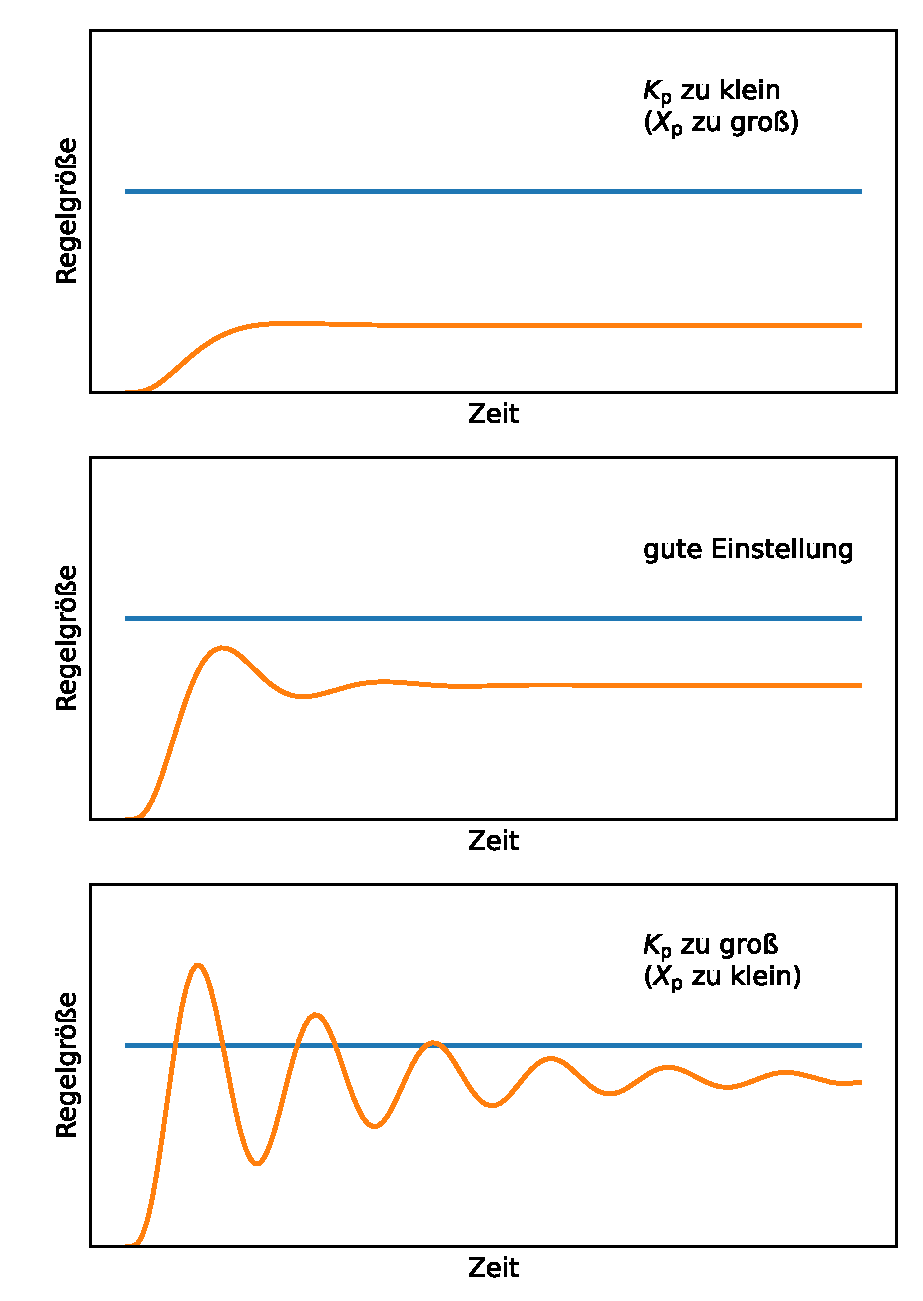
\includegraphics[width=\textwidth]{Abbildungen/tlk_p_anteil.pdf}
        \caption{Proportionalanteil}
        \label{subfig:tlk_p}
    \end{subfigure}
    \hfill % Schiebt das nächste Bild elastisch nach rechts
    
    % --- Mittleres Bild: I-Anteil (b) ---
    \begin{subfigure}[b]{0.31\textwidth}
        \centering
        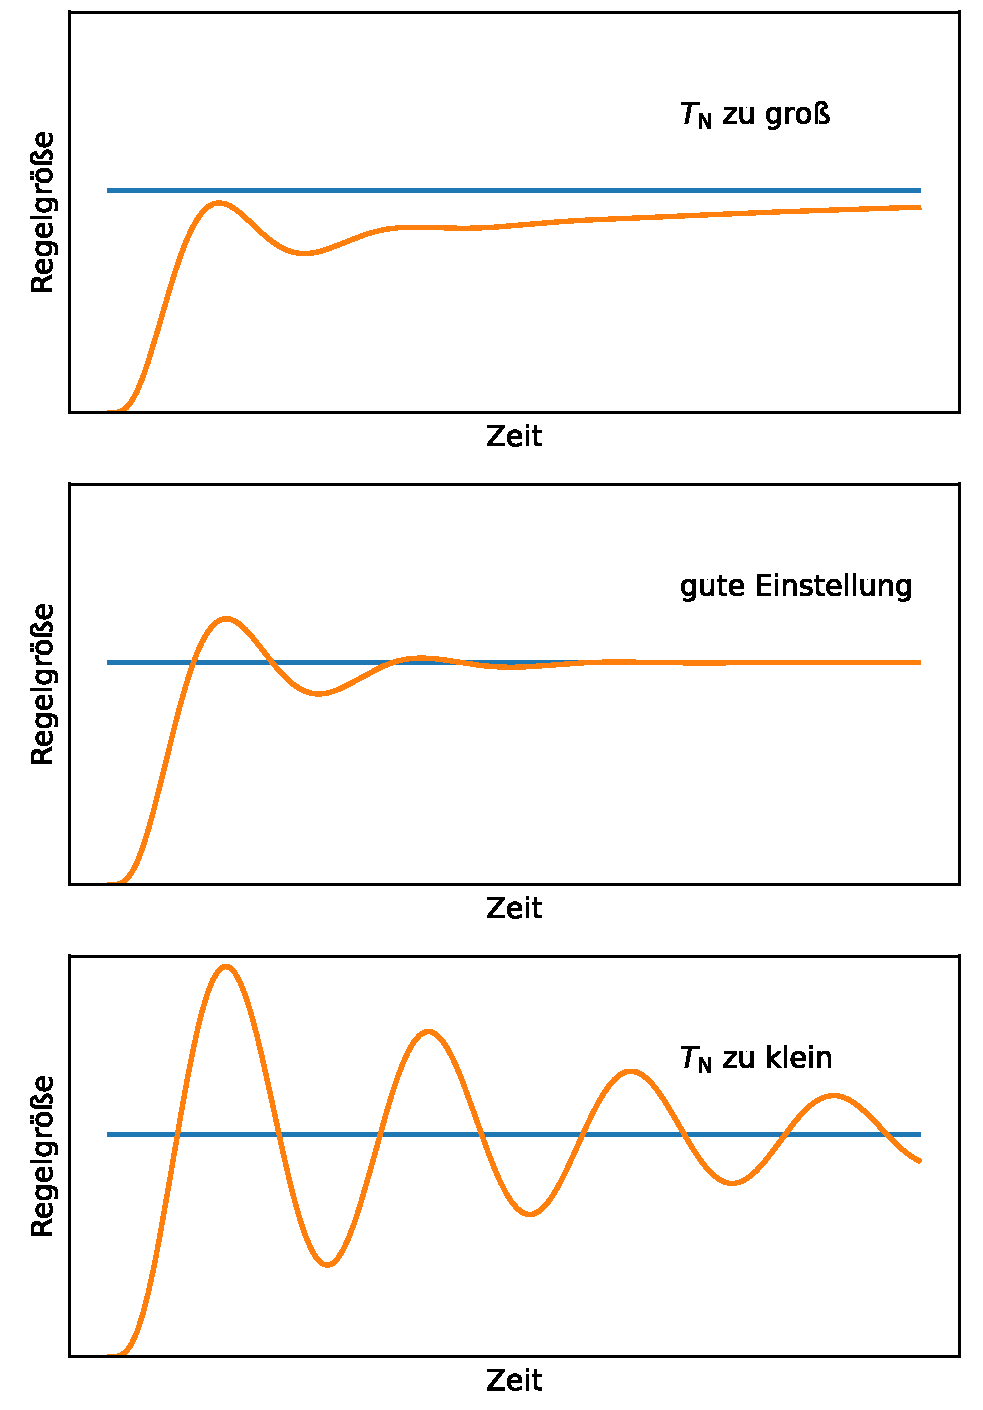
\includegraphics[width=\textwidth]{Abbildungen/tlk_i_anteil.pdf}
        \caption{Integralanteil}
        \label{subfig:tlk_i}
    \end{subfigure}
    \hfill % Schiebt das nächste Bild elastisch nach rechts
    
    % --- Rechtes Bild: D-Anteil (c) ---
    \begin{subfigure}[b]{0.38\textwidth}
        \centering
        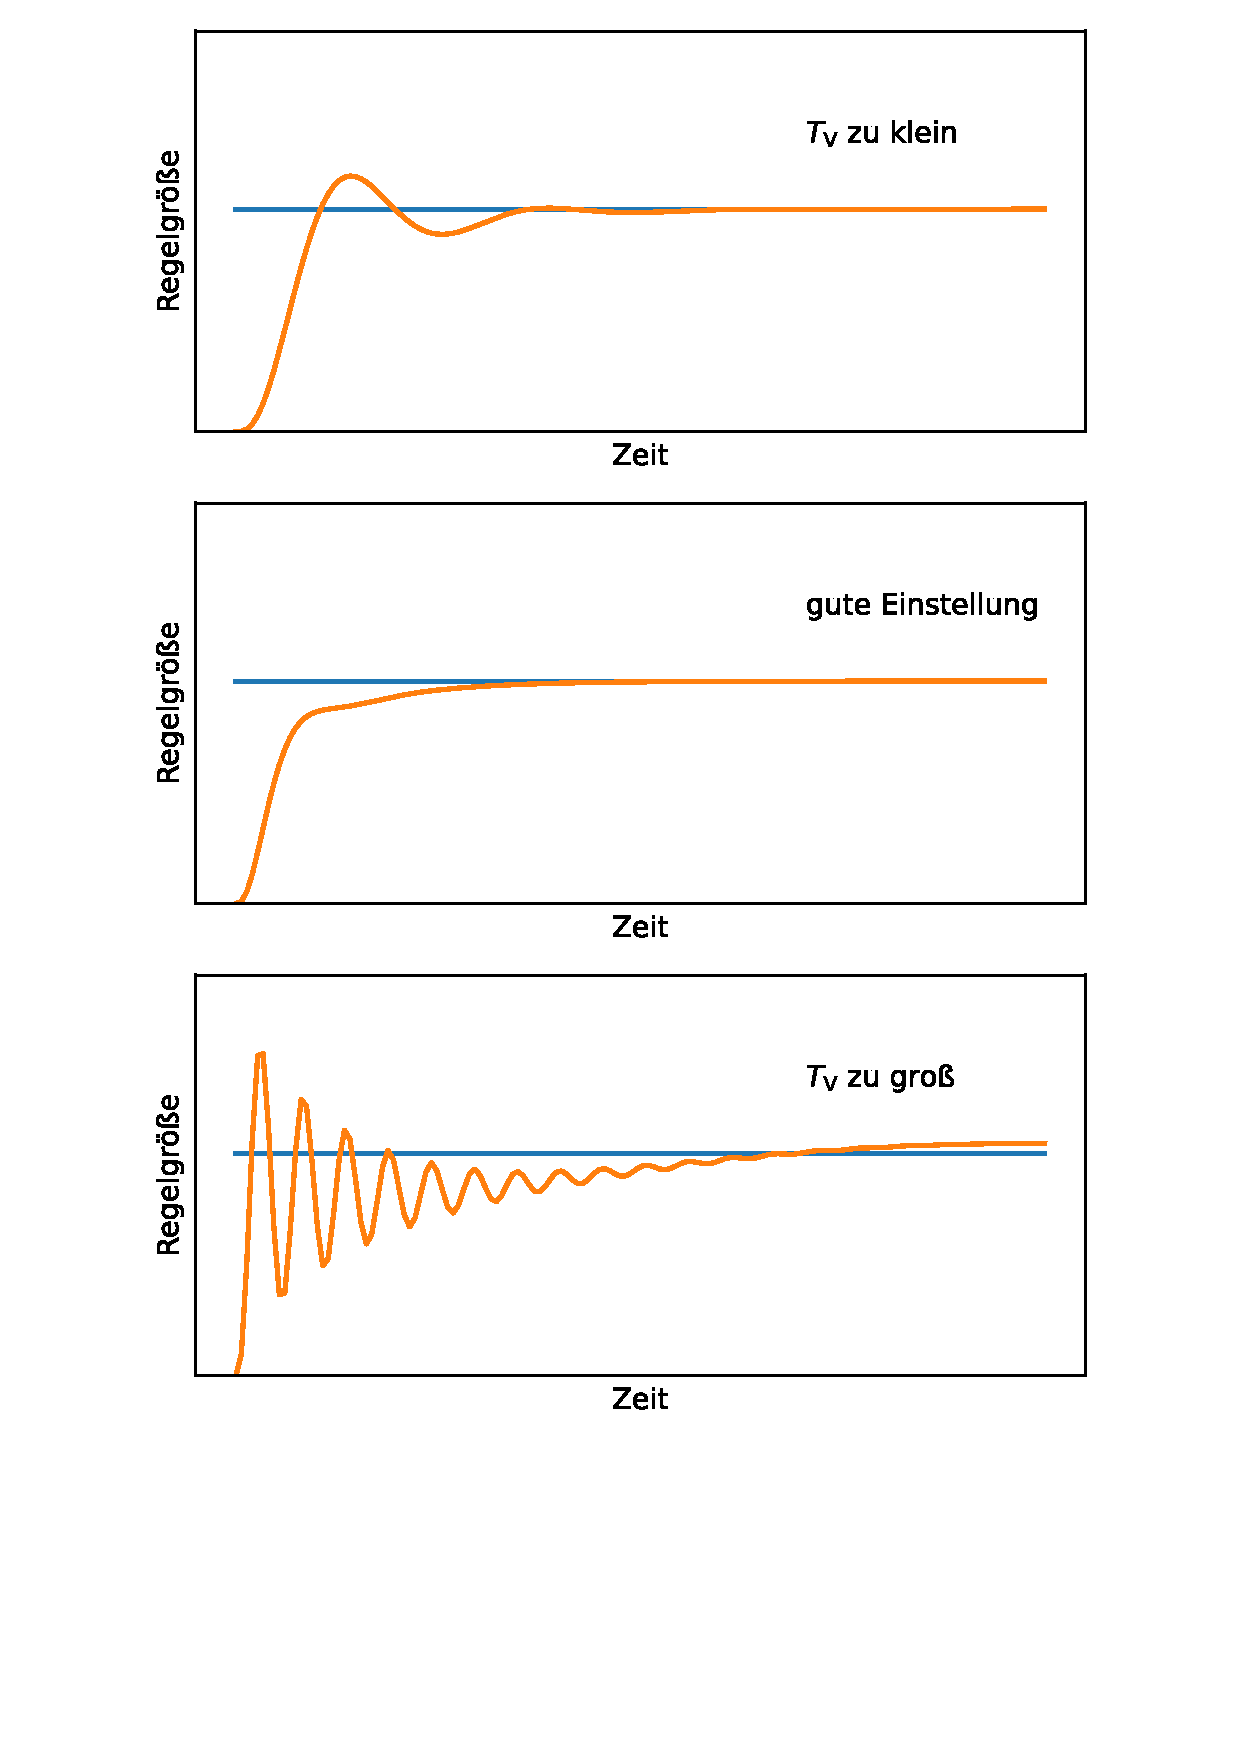
\includegraphics[width=\textwidth]{Abbildungen/tlk_d_anteil.pdf}
        \caption{Differenzialanteil}
        \label{subfig:tlk_d}
    \end{subfigure}

    % Hauptüberschrift unter allen drei Bildern
    \caption{\small {Vergleich der Reglerparameter (P-, I- und D-Anteil).}}
    \label{fig:regler_parameter_vergleich} % Referenz für den Fließtext
\end{figure}


\subsection{Aufgabe A -- Regler-Einstellung mit Trial-and-Error}

Gegeben ist die Regelstrecke

\begin{equation}
G_S(s)=\frac{1}{2+0.5s} \cdot e^{-0.3s}
\end{equation}

mit der Totzeit

\begin{equation}
T_t = 0.3\,\mathrm{s}.
\end{equation}

Mithilfe des Trial-and-Error-Verfahrens ist ein PID-Regler in Simulink so zu parametrisieren, dass das System möglichst schnell auf einen Eingangssprung reagiert.

\subsubsection{Versuchsaufbau und Durchführung}
Zuerst werden in MATLAB die Variablen für die Strecke definiert. 

\begin{lstlisting}[language=Matlab, caption={MATLAB-Skript zur Streckendefinition und Stabilitätsanalyse.}]
Gs = tf(1, [0.5, 2], 'IoDelay', 0.3); % Definition der Regelstrecke
s = tf('s');
\end{lstlisting}

\begin{figure}[htbp]
    \centering
    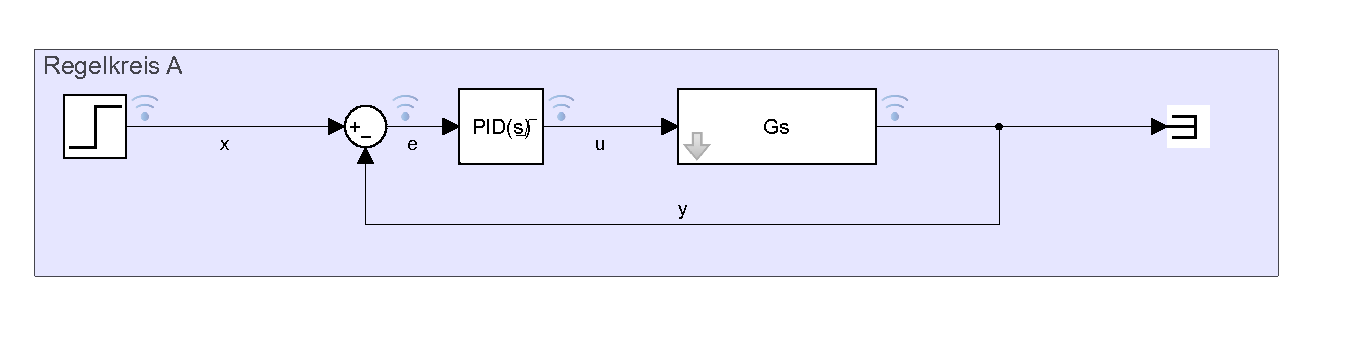
\includegraphics[width=1\textwidth]{Abbildungen/regelkreis_7_A1.pdf}
    \caption{Regelkreises in Simulink}
    \label{fig:simulink_circuit}
\end{figure}

Die Einstellregel nach dem Trial-and-Error-Verfahren erfolgt schrittweise, beginnend mit dem Proportionalanteil ($P$), während der Integral- ($I$) und Derivativanteil ($D$) zunächst auf Null gesetzt bleiben.

\paragraph{P-Anteils:}
Zuerst wird ein niedriger Proportionalwert von $P = 1$ gewählt.
Beim vergleich von Abbildung~\ref{fig:step_response_P1} mit Abbildung~\ref{subfig:tlk_p}, wird ersichtlich, dass $P$ zu niedrig gewählt wurde.

\begin{figure}[H]
    \centering
    
    \input{Abbildungen/step_resp_aufgabe_7A_1.tikz}
    \caption{Sprungantwort des Regelkreises mit reinem P-Regler ($P=1$).}
    \label{fig:step_response_P1}
\end{figure}

Es erfolgt eine Steigerung auf $P = 1.3$.

\begin{figure}[H]
    \centering

    % This file was created by matlab2tikz.
%
%The latest updates can be retrieved from
%  http://www.mathworks.com/matlabcentral/fileexchange/22022-matlab2tikz-matlab2tikz
%where you can also make suggestions and rate matlab2tikz.
%
\definecolor{mycolor1}{rgb}{0.00000,0.44700,0.74100}%
\definecolor{mycolor2}{rgb}{0.92900,0.69400,0.12500}%
\definecolor{mycolor3}{rgb}{0.12941,0.12941,0.12941}%
%
\begin{tikzpicture}

\begin{axis}[%
width=0.951\figurewidth,
height=\figureheight,
at={(0\figurewidth,0\figureheight)},
scale only axis,
xmin=0,
xmax=10.4,
tick align=outside,
xlabel style={font=\color{mycolor3}},
xlabel={Time (seconds)},
ymin=-0.05,
ymax=1.05,
axis background/.style={fill=white},
xmajorgrids,
ymajorgrids,
legend style={at={(0.14,0.935)}, anchor=south west, legend cell align=left, align=left}
]
\addplot [color=mycolor1, line width=2.0pt]
  table[row sep=crcr]{%
0	0\\
0.01	0\\
0.02	0\\
0.03	0\\
0.04	0\\
0.05	0\\
0.06	0\\
0.07	0\\
0.08	0\\
0.09	0\\
0.1	0\\
0.11	0\\
0.12	0\\
0.13	0\\
0.14	0\\
0.15	0\\
0.16	0\\
0.17	0\\
0.18	0\\
0.19	0\\
0.2	0\\
0.21	0\\
0.22	0\\
0.23	0\\
0.24	0\\
0.25	0\\
0.26	0\\
0.27	0\\
0.28	0\\
0.29	0\\
0.3	0\\
0.31	0\\
0.32	0\\
0.33	0\\
0.34	0\\
0.35	0\\
0.36	0\\
0.37	0\\
0.38	0\\
0.39	0\\
0.4	0\\
0.41	0\\
0.42	0\\
0.43	0\\
0.44	0\\
0.45	0\\
0.46	0\\
0.47	0\\
0.48	0\\
0.49	0\\
0.5	0\\
0.51	0\\
0.52	0\\
0.53	0\\
0.54	0\\
0.55	0\\
0.56	0\\
0.57	0\\
0.58	0\\
0.59	0\\
0.6	0\\
0.61	0\\
0.62	0\\
0.63	0\\
0.64	0\\
0.65	0\\
0.66	0\\
0.67	0\\
0.68	0\\
0.69	0\\
0.7	0\\
0.71	0\\
0.72	0\\
0.73	0\\
0.74	0\\
0.75	0\\
0.76	0\\
0.77	0\\
0.78	0\\
0.79	0\\
0.8	0\\
0.81	0\\
0.820000000000001	0\\
0.830000000000001	0\\
0.840000000000001	0\\
0.850000000000001	0\\
0.860000000000001	0\\
0.870000000000001	0\\
0.880000000000001	0\\
0.890000000000001	0\\
0.900000000000001	0\\
0.910000000000001	0\\
0.920000000000001	0\\
0.930000000000001	0\\
0.940000000000001	0\\
0.950000000000001	0\\
0.960000000000001	0\\
0.970000000000001	0\\
0.980000000000001	0\\
0.990000000000001	0\\
0.999999999999994	0\\
1	0\\
1.01	0\\
1.02	0\\
1.03	0\\
1.04	0\\
1.05	0\\
1.06	0\\
1.07	0\\
1.08	0\\
1.09	0\\
1.1	0\\
1.11	0\\
1.12	0\\
1.13	0\\
1.14	0\\
1.15	0\\
1.16	0\\
1.17	0\\
1.18	0\\
1.19	0\\
1.2	0\\
1.21	0\\
1.22	0\\
1.23	0\\
1.24	0\\
1.25	0\\
1.26	0\\
1.27	0\\
1.28	0\\
1.29	0\\
1.3	5.65922076983346e-16\\
1.31	0.0254868645502299\\
1.32	0.0499743748472257\\
1.33	0.0735017161317418\\
1.34	0.0961065371692648\\
1.35	0.117825010496072\\
1.36	0.138691890303004\\
1.37	0.158740568049591\\
1.38	0.178003125897503\\
1.39	0.19651038804886\\
1.4	0.214291970071528\\
1.41	0.23137632629035\\
1.42	0.247790795320131\\
1.43	0.263561643813256\\
1.44	0.27871410849194\\
1.45	0.293272436532366\\
1.46	0.30725992436534\\
1.47	0.320698954955549\\
1.48	0.333611033619083\\
1.49	0.346016822436525\\
1.5	0.357936173316692\\
1.51	0.369388159763922\\
1.52	0.380391107399749\\
1.53	0.39096262328781\\
1.54	0.401119624108903\\
1.55	0.410878363231282\\
1.56	0.420254456719518\\
1.57	0.429262908323531\\
1.58	0.437918133487792\\
1.59	0.44623398241911\\
1.6	0.454223762249916\\
1.61	0.46157330298991\\
1.62	0.467997903953278\\
1.63	0.473558800270498\\
1.64	0.478313847009811\\
1.65	0.482317690098439\\
1.66	0.485621929036698\\
1.67	0.488275271785848\\
1.68	0.490323682193242\\
1.69	0.491810520301881\\
1.7	0.492776675875727\\
1.71	0.493260695457067\\
1.72	0.493298903257886\\
1.73	0.49292551617342\\
1.74	0.492172753192981\\
1.75	0.491070939470599\\
1.76	0.48964860530604\\
1.77	0.487932580275337\\
1.78	0.485948082739023\\
1.79	0.483718804945844\\
1.8	0.481266993939733\\
1.81	0.478613528468314\\
1.82	0.475777992082116\\
1.83	0.472778742604972\\
1.84	0.469632978147799\\
1.85	0.466356799830016\\
1.86	0.462965271365304\\
1.87	0.459472475661165\\
1.88	0.455891568574869\\
1.89	0.452234829961752\\
1.9	0.448513712145555\\
1.91	0.444743080243918\\
1.92	0.440944845669252\\
1.93	0.437142879004743\\
1.94	0.433358597523895\\
1.95	0.429611145340716\\
1.96	0.425917562245164\\
1.97	0.42229294187178\\
1.98	0.41875057981457\\
1.99	0.415302112268102\\
2	0.411957645743375\\
2.01	0.408725878377304\\
2.02	0.405614213326385\\
2.03	0.4026288647084\\
2.04	0.399774956530621\\
2.05	0.397056615018954\\
2.06	0.394477054739665\\
2.07	0.392038658883729\\
2.08	0.38974305406339\\
2.09	0.387591179951127\\
2.1	0.385583354072844\\
2.11	0.383719332049715\\
2.12	0.381998363566621\\
2.13	0.380419244329514\\
2.14	0.378980364259268\\
2.15	0.37767975215557\\
2.16	0.376515117051168\\
2.17	0.37548388646425\\
2.18	0.374583241744863\\
2.19	0.373810150700038\\
2.2	0.373161397671677\\
2.21	0.372633557424979\\
2.22	0.372222869772687\\
2.23	0.371925138380399\\
2.24	0.371735754540021\\
2.25	0.371649773555305\\
2.26	0.371661983685961\\
2.27	0.371766968222171\\
2.28	0.371959161222887\\
2.29	0.372232897415143\\
2.29999999999999	0.372582456717764\\
2.30999999999999	0.373002103821051\\
2.31999999999999	0.37348612322429\\
2.32999999999999	0.374028850104955\\
2.33999999999999	0.37462469736737\\
2.34999999999999	0.375268179194057\\
2.35999999999999	0.375953931400083\\
2.36999999999999	0.376676728869199\\
2.37999999999999	0.377431500330516\\
2.38999999999999	0.378213340715602\\
2.39999999999999	0.379017521318341\\
2.40999999999999	0.379839497963429\\
2.41999999999999	0.380674917374016\\
2.42999999999999	0.38151962191468\\
2.43999999999999	0.382369652872461\\
2.44999999999999	0.383221252426225\\
2.45999999999999	0.384070864442921\\
2.46999999999999	0.38491513422842\\
2.47999999999999	0.385750907350465\\
2.48999999999999	0.386575227641822\\
2.49999999999999	0.387385334482882\\
2.50999999999999	0.388178660145053\\
2.51999999999999	0.388952829177219\\
2.52999999999999	0.389705660701477\\
2.53999999999999	0.390435171594869\\
2.54999999999999	0.391139578265504\\
2.55999999999999	0.391817296507677\\
2.56999999999999	0.392466939693625\\
2.57999999999999	0.393087315535381\\
2.58999999999999	0.393677421627912\\
2.59999999999999	0.394236439964196\\
2.60999999999999	0.394763730594014\\
2.61999999999999	0.395258824580901\\
2.62999999999999	0.395721416395724\\
2.63999999999999	0.396151355870775\\
2.64999999999999	0.396548639824821\\
2.65999999999999	0.396913403457302\\
2.66999999999999	0.397245911598645\\
2.67999999999999	0.397546549893365\\
2.68999999999999	0.397815815983327\\
2.69999999999999	0.398054310749949\\
2.70999999999999	0.398262729666412\\
2.71999999999999	0.398441854303864\\
2.72999999999999	0.398592544029226\\
2.73999999999999	0.398715727926393\\
2.74999999999999	0.398812396967426\\
2.75999999999999	0.398883596455558\\
2.76999999999998	0.398930418757645\\
2.77999999999998	0.39895399633982\\
2.78999999999998	0.398955495116754\\
2.79999999999998	0.398936108121822\\
2.80999999999998	0.39889704949395\\
2.81999999999998	0.398839548741735\\
2.82999999999998	0.398764845210795\\
2.83999999999998	0.398674182698173\\
2.84999999999998	0.398568804214856\\
2.85999999999998	0.398449946933037\\
2.86999999999998	0.398318837356523\\
2.87999999999998	0.398176686744945\\
2.88999999999998	0.398024686815558\\
2.89999999999998	0.397864005740345\\
2.90999999999998	0.397695784450863\\
2.91999999999998	0.397521133258599\\
2.92999999999998	0.397341128794569\\
2.93999999999998	0.397156811268429\\
2.94999999999998	0.396969182044334\\
2.95999999999998	0.396779201528268\\
2.96999999999998	0.396587787359391\\
2.97999999999998	0.396395812896172\\
2.98999999999998	0.396204105986588\\
2.99999999999998	0.396013448010505\\
3.00999999999998	0.395824573181404\\
3.01999999999998	0.395638168093914\\
3.02999999999998	0.395454871503111\\
3.03999999999998	0.395275274321204\\
3.04999999999998	0.39509991981704\\
3.05999999999998	0.394929304003838\\
3.06999999999998	0.394763876200609\\
3.07999999999998	0.394604039752899\\
3.08999999999998	0.394450152898745\\
3.09999999999998	0.394302529766072\\
3.10999999999998	0.394161441488246\\
3.11999999999998	0.394027117425574\\
3.12999999999998	0.393899746482507\\
3.13999999999998	0.39377947851231\\
3.14999999999998	0.393666425802011\\
3.15999999999998	0.393560664630252\\
3.16999999999998	0.393462236889964\\
3.17999999999998	0.393371151767257\\
3.18999999999998	0.393287387467532\\
3.19999999999998	0.393210892979681\\
3.20999999999998	0.393141589869181\\
3.21999999999998	0.393079374091009\\
3.22999999999998	0.393024117813511\\
3.23999999999997	0.392975671244663\\
3.24999999999997	0.392933864452515\\
3.25999999999997	0.392898509172036\\
3.26999999999997	0.392869400591065\\
3.27999999999997	0.392846319108547\\
3.28999999999997	0.392829032058763\\
3.29999999999997	0.392817295395811\\
3.30999999999997	0.392810855333109\\
3.31999999999997	0.392809449933265\\
3.32999999999997	0.392812810644157\\
3.33999999999997	0.392820663777626\\
3.34999999999997	0.392832731927667\\
3.35999999999997	0.392848735325515\\
3.36999999999997	0.392868393129483\\
3.37999999999997	0.392891424647879\\
3.38999999999997	0.392917550493729\\
3.39999999999997	0.392946493670481\\
3.40999999999997	0.392977980588184\\
3.41999999999997	0.393011742010047\\
3.42999999999997	0.393047513929511\\
3.43999999999997	0.393085038378244\\
3.44999999999997	0.393124064165622\\
3.45999999999997	0.393164347550432\\
3.46999999999997	0.393205652845698\\
3.47999999999997	0.393247752957721\\
3.48999999999997	0.39329042986058\\
3.49999999999997	0.39333347500755\\
3.50999999999997	0.393376689681049\\
3.51999999999997	0.393419885282917\\
3.52999999999997	0.393462883566959\\
3.53999999999997	0.393505516815855\\
3.54999999999997	0.393547627964669\\
3.55999999999997	0.393589070673286\\
3.56999999999997	0.393629709350226\\
3.57999999999997	0.393669419130364\\
3.58999999999997	0.393708085809149\\
3.59999999999997	0.393745605735963\\
3.60999999999997	0.393781885669309\\
3.61999999999997	0.393816842596527\\
3.62999999999997	0.39385040352075\\
3.63999999999997	0.393882505217796\\
3.64999999999997	0.393913093965687\\
3.65999999999997	0.393942125249433\\
3.66999999999997	0.393969563443695\\
3.67999999999997	0.393995381475872\\
3.68999999999997	0.394019560472111\\
3.69999999999997	0.394042089388643\\
3.70999999999996	0.394062964630805\\
3.71999999999996	0.39408218966199\\
3.72999999999996	0.394099774604694\\
3.73999999999996	0.394115735835743\\
3.74999999999996	0.394130095577678\\
3.75999999999996	0.394142881488174\\
3.76999999999996	0.394154126249315\\
3.77999999999996	0.394163867158384\\
3.78999999999996	0.394172145721796\\
3.79999999999996	0.394179007253673\\
3.80999999999996	0.394184500480455\\
3.81999999999996	0.394188677152863\\
3.82999999999996	0.394191591666418\\
3.83999999999996	0.394193300691632\\
3.84999999999996	0.394193862814871\\
3.85999999999996	0.394193338190806\\
3.86999999999996	0.394191788207272\\
3.87999999999996	0.394189275163254\\
3.88999999999996	0.394185861960621\\
3.89999999999996	0.39418161181015\\
3.90999999999996	0.394176587952285\\
3.91999999999996	0.394170853392991\\
3.92999999999996	0.39416447065498\\
3.93999999999996	0.394157501544505\\
3.94999999999996	0.394150006933853\\
3.95999999999996	0.394142046559565\\
3.96999999999996	0.394133678836389\\
3.97999999999996	0.394124960686855\\
3.98999999999996	0.394115947386351\\
3.99999999999996	0.394106692423473\\
4.00999999999996	0.394097247375409\\
4.01999999999996	0.394087661798051\\
4.02999999999996	0.394077983130481\\
4.03999999999996	0.394068256613441\\
4.04999999999996	0.394058525221377\\
4.05999999999996	0.394048829607573\\
4.06999999999996	0.394039208061915\\
4.07999999999996	0.394029696480749\\
4.08999999999996	0.39402032834832\\
4.09999999999996	0.394011134729221\\
4.10999999999996	0.394002144271296\\
4.11999999999996	0.39399338321841\\
4.12999999999996	0.393984875432498\\
4.13999999999996	0.393976642424301\\
4.14999999999996	0.39396870339218\\
4.15999999999996	0.393961075268417\\
4.16999999999996	0.393953772772395\\
4.17999999999996	0.393946808470069\\
4.18999999999996	0.393940192839138\\
4.19999999999995	0.39393393433933\\
4.20999999999995	0.393928039487236\\
4.21999999999995	0.393922512935136\\
4.22999999999995	0.393917357553267\\
4.23999999999995	0.393912574515003\\
4.24999999999995	0.393908163384447\\
4.25999999999995	0.393904122205915\\
4.26999999999995	0.393900447594871\\
4.27999999999995	0.393897134829818\\
4.28999999999995	0.393894177944748\\
4.29999999999995	0.393891569821707\\
4.30999999999995	0.393889302283105\\
4.31999999999995	0.393887366183388\\
4.32999999999995	0.393885751499736\\
4.33999999999995	0.393884447421456\\
4.34999999999995	0.393883442437778\\
4.35999999999995	0.393882724423768\\
4.36999999999995	0.393882280724111\\
4.37999999999995	0.39388209823453\\
4.38999999999995	0.393882163480633\\
4.39999999999995	0.393882462693997\\
4.40999999999995	0.393882981885333\\
4.41999999999995	0.393883706914572\\
4.42999999999995	0.393884623557769\\
4.43999999999995	0.393885717570705\\
4.44999999999995	0.393886974749107\\
4.45999999999995	0.393888380985422\\
4.46999999999995	0.393889922322101\\
4.47999999999995	0.393891585001352\\
4.48999999999995	0.393893355511356\\
4.49999999999995	0.393895220628943\\
4.50999999999995	0.393897167458747\\
4.51999999999995	0.393899183468865\\
4.52999999999995	0.393901256523065\\
4.53999999999995	0.393903374909599\\
4.54999999999995	0.393905527366682\\
4.55999999999995	0.393907703104715\\
4.56999999999995	0.39390989182534\\
4.57999999999995	0.393912083737415\\
4.58999999999995	0.393914269570017\\
4.59999999999995	0.393916440582572\\
4.60999999999995	0.393918588572237\\
4.61999999999995	0.393920705878646\\
4.62999999999995	0.393922785386145\\
4.63999999999995	0.393924820523646\\
4.64999999999995	0.39392680526223\\
4.65999999999995	0.393928734110626\\
4.66999999999994	0.39393060210871\\
4.67999999999994	0.393932404819151\\
4.68999999999994	0.393934138317342\\
4.69999999999994	0.393935799179756\\
4.70999999999994	0.393937384470851\\
4.71999999999994	0.393938891728665\\
4.72999999999994	0.393940318949236\\
4.73999999999994	0.393941664569958\\
4.74999999999994	0.393942927452029\\
4.75999999999994	0.393944106862076\\
4.76999999999994	0.393945202453121\\
4.77999999999994	0.393946214244957\\
4.78999999999994	0.393947142604093\\
4.79999999999994	0.393947988223335\\
4.80999999999994	0.393948752101137\\
4.81999999999994	0.393949435520803\\
4.82999999999994	0.39395004002964\\
4.83999999999994	0.393950567418154\\
4.84999999999994	0.393951019699368\\
4.85999999999994	0.393951399088343\\
4.86999999999994	0.393951707981977\\
4.87999999999994	0.393951948939151\\
4.88999999999994	0.393952124661283\\
4.89999999999994	0.393952237973349\\
4.90999999999994	0.39395229180543\\
4.91999999999994	0.393952289174819\\
4.92999999999994	0.393952233168753\\
4.93999999999994	0.393952126927786\\
4.94999999999994	0.39395197362985\\
4.95999999999994	0.39395177647503\\
4.96999999999994	0.393951538671074\\
4.97999999999994	0.393951263419665\\
4.98999999999994	0.393950953903464\\
4.99999999999994	0.393950613273932\\
5.00999999999994	0.393950244639958\\
5.01999999999994	0.39394985105727\\
5.02999999999994	0.393949435518654\\
5.03999999999994	0.393949000944956\\
5.04999999999994	0.393948550176887\\
5.05999999999994	0.393948085967594\\
5.06999999999994	0.393947610976007\\
5.07999999999994	0.393947127760933\\
5.08999999999994	0.3939466387759\\
5.09999999999994	0.393946146364699\\
5.10999999999994	0.393945652757646\\
5.11999999999994	0.3939451600685\\
5.12999999999994	0.393944670292045\\
5.13999999999993	0.393944185302295\\
5.14999999999993	0.393943706851291\\
5.15999999999993	0.393943236568478\\
5.16999999999993	0.393942775960625\\
5.17999999999993	0.393942326412248\\
5.18999999999993	0.393941889186534\\
5.19999999999993	0.393941465426698\\
5.20999999999993	0.393941056157787\\
5.21999999999993	0.393940662288853\\
5.22999999999993	0.393940284615509\\
5.23999999999993	0.393939923822799\\
5.24999999999993	0.393939580488388\\
5.25999999999993	0.393939255086009\\
5.26999999999993	0.393938947989161\\
5.27999999999993	0.393938659475019\\
5.28999999999993	0.393938389728537\\
5.29999999999993	0.393938138846696\\
5.30999999999993	0.393937906842904\\
5.31999999999993	0.393937693651487\\
5.32999999999993	0.393937499132272\\
5.33999999999993	0.393937323075231\\
5.34999999999993	0.393937165205154\\
5.35999999999993	0.393937025186345\\
5.36999999999993	0.39393690262731\\
5.37999999999993	0.393936797085425\\
5.38999999999993	0.393936708071552\\
5.39999999999993	0.393936635054611\\
5.40999999999993	0.393936577466063\\
5.41999999999993	0.393936534704316\\
5.42999999999993	0.393936506139017\\
5.43999999999993	0.39393649111524\\
5.44999999999993	0.39393648895754\\
5.45999999999993	0.393936498973876\\
5.46999999999993	0.393936520459386\\
5.47999999999993	0.393936552700012\\
5.48999999999993	0.393936594975964\\
5.49999999999993	0.393936646565018\\
5.50999999999993	0.393936706745652\\
5.51999999999993	0.393936774799993\\
5.52999999999993	0.393936850016607\\
5.53999999999993	0.393936931693093\\
5.54999999999993	0.393937019138511\\
5.55999999999993	0.393937111675624\\
5.56999999999993	0.393937208642961\\
5.57999999999993	0.393937309396704\\
5.58999999999993	0.393937413312398\\
5.59999999999993	0.393937519786488\\
5.60999999999992	0.393937628237687\\
5.61999999999992	0.39393773810817\\
5.62999999999992	0.393937848864616\\
5.63999999999992	0.393937959999085\\
5.64999999999992	0.393938071029741\\
5.65999999999992	0.393938181501434\\
5.66999999999992	0.393938290986129\\
5.67999999999992	0.393938399083211\\
5.68999999999992	0.393938505419649\\
5.69999999999992	0.393938609650046\\
5.70999999999992	0.393938711456562\\
5.71999999999992	0.393938810548735\\
5.72999999999992	0.393938906663194\\
5.73999999999992	0.393938999563275\\
5.74999999999992	0.39393908903855\\
5.75999999999992	0.393939174904268\\
5.76999999999992	0.393939257000728\\
5.77999999999992	0.393939335192571\\
5.78999999999992	0.393939409368018\\
5.79999999999992	0.39393947943805\\
5.80999999999992	0.393939545335538\\
5.81999999999992	0.393939607014326\\
5.82999999999992	0.393939664448282\\
5.83999999999992	0.393939717630314\\
5.84999999999992	0.393939766571366\\
5.85999999999992	0.393939811299384\\
5.86999999999992	0.393939851858278\\
5.87999999999992	0.393939888306868\\
5.88999999999992	0.393939920717829\\
5.89999999999992	0.393939949176632\\
5.90999999999992	0.393939973780496\\
5.91999999999992	0.39393999463734\\
5.92999999999992	0.393940011864757\\
5.93999999999992	0.393940025588992\\
5.94999999999992	0.393940035943956\\
5.95999999999992	0.393940043070242\\
5.96999999999992	0.393940047114188\\
5.97999999999992	0.393940048226947\\
5.98999999999992	0.393940046563605\\
5.99999999999992	0.393940042282318\\
6.00999999999992	0.393940035543492\\
6.01999999999992	0.39394002650899\\
6.02999999999992	0.393940015341387\\
6.03999999999992	0.39394000220325\\
6.04999999999992	0.393939987256471\\
6.05999999999992	0.393939970661623\\
6.06999999999992	0.393939952577375\\
6.07999999999991	0.393939933159928\\
6.08999999999991	0.39393991256251\\
6.09999999999991	0.393939890934894\\
6.10999999999991	0.393939868422971\\
6.11999999999991	0.393939845168351\\
6.12999999999991	0.393939821308014\\
6.13999999999991	0.393939796973987\\
6.14999999999991	0.393939772293074\\
6.15999999999991	0.393939747386605\\
6.16999999999991	0.393939722370239\\
6.17999999999991	0.393939697353788\\
6.18999999999991	0.393939672441082\\
6.19999999999991	0.393939647729864\\
6.20999999999991	0.393939623311713\\
6.21999999999991	0.393939599272004\\
6.22999999999991	0.39393957568989\\
6.23999999999991	0.393939552638312\\
6.24999999999991	0.393939530184033\\
6.25999999999991	0.393939508387702\\
6.26999999999991	0.393939487303932\\
6.27999999999991	0.393939466981404\\
6.28999999999991	0.393939447462986\\
6.29999999999991	0.393939428785873\\
6.30999999999991	0.393939410981743\\
6.31999999999991	0.393939394076924\\
6.32999999999991	0.393939378092578\\
6.33999999999991	0.393939363044893\\
6.34999999999991	0.393939348945289\\
6.35999999999991	0.393939335800626\\
6.36999999999991	0.39393932361343\\
6.37999999999991	0.393939312382114\\
6.38999999999991	0.393939302101212\\
6.39999999999991	0.393939292761609\\
6.40999999999991	0.393939284350781\\
6.41999999999991	0.393939276853033\\
6.42999999999991	0.393939270249733\\
6.43999999999991	0.393939264519554\\
6.44999999999991	0.393939259638707\\
6.45999999999991	0.393939255581173\\
6.46999999999991	0.393939252318935\\
6.47999999999991	0.393939249822201\\
6.48999999999991	0.393939248059625\\
6.49999999999991	0.393939246998523\\
6.50999999999991	0.393939246605079\\
6.51999999999991	0.393939246844549\\
6.52999999999991	0.393939247681457\\
6.53999999999991	0.393939249079777\\
6.5499999999999	0.393939251003118\\
6.5599999999999	0.393939253414893\\
6.5699999999999	0.393939256278479\\
6.5799999999999	0.393939259557377\\
6.5899999999999	0.393939263215349\\
6.5999999999999	0.393939267216561\\
6.6099999999999	0.393939271525705\\
6.6199999999999	0.39393927610812\\
6.6299999999999	0.393939280929898\\
6.6399999999999	0.393939285957987\\
6.6499999999999	0.393939291160278\\
6.6599999999999	0.393939296505688\\
6.6699999999999	0.393939301964235\\
6.6799999999999	0.393939307507101\\
6.6899999999999	0.393939313106686\\
6.6999999999999	0.393939318736661\\
6.7099999999999	0.393939324372005\\
6.7199999999999	0.393939329989035\\
6.7299999999999	0.393939335565439\\
6.7399999999999	0.393939341080285\\
6.7499999999999	0.393939346514039\\
6.7599999999999	0.393939351848569\\
6.7699999999999	0.39393935706714\\
6.7799999999999	0.393939362154413\\
6.7899999999999	0.393939367096426\\
6.7999999999999	0.393939371880584\\
6.8099999999999	0.393939376495632\\
6.8199999999999	0.393939380931629\\
6.8299999999999	0.393939385179921\\
6.8399999999999	0.393939389233103\\
6.8499999999999	0.393939393084983\\
6.8599999999999	0.393939396730544\\
6.8699999999999	0.393939400165895\\
6.8799999999999	0.393939403388232\\
6.8899999999999	0.393939406395788\\
6.8999999999999	0.393939409187783\\
6.9099999999999	0.393939411764374\\
6.9199999999999	0.393939414126602\\
6.9299999999999	0.393939416276345\\
6.9399999999999	0.393939418216256\\
6.9499999999999	0.393939419949717\\
6.9599999999999	0.393939421480782\\
6.9699999999999	0.393939422814124\\
6.9799999999999	0.393939423954982\\
6.9899999999999	0.393939424909108\\
6.9999999999999	0.393939425682717\\
7.00999999999989	0.393939426282433\\
7.01999999999989	0.393939426715242\\
7.02999999999989	0.39393942698844\\
7.03999999999989	0.393939427109591\\
7.04999999999989	0.393939427086476\\
7.05999999999989	0.39393942692705\\
7.06999999999989	0.393939426639403\\
7.07999999999989	0.393939426231714\\
7.08999999999989	0.393939425712216\\
7.09999999999989	0.393939425089155\\
7.10999999999989	0.393939424370762\\
7.11999999999989	0.393939423565211\\
7.12999999999989	0.393939422680595\\
7.13999999999989	0.393939421724892\\
7.14999999999989	0.393939420705942\\
7.15999999999989	0.39393941963142\\
7.16999999999989	0.393939418508814\\
7.17999999999989	0.393939417345402\\
7.18999999999989	0.393939416148236\\
7.19999999999989	0.393939414924123\\
7.20999999999989	0.393939413679613\\
7.21999999999989	0.393939412420982\\
7.22999999999989	0.393939411154222\\
7.23999999999989	0.393939409885034\\
7.24999999999989	0.393939408618818\\
7.25999999999989	0.393939407360667\\
7.26999999999989	0.393939406115363\\
7.27999999999989	0.393939404887375\\
7.28999999999989	0.393939403680855\\
7.29999999999989	0.393939402499642\\
7.30999999999989	0.393939401347259\\
7.31999999999989	0.393939400226917\\
7.32999999999989	0.393939399141521\\
7.33999999999989	0.393939398093672\\
7.34999999999989	0.393939397085673\\
7.35999999999989	0.393939396119536\\
7.36999999999989	0.393939395196989\\
7.37999999999989	0.393939394319487\\
7.38999999999989	0.393939393488218\\
7.39999999999989	0.393939392704112\\
7.40999999999989	0.393939391967854\\
7.41999999999989	0.393939391279893\\
7.42999999999989	0.393939390640453\\
7.43999999999989	0.393939390049543\\
7.44999999999989	0.393939389506973\\
7.45999999999989	0.393939389012359\\
7.46999999999989	0.393939388565143\\
7.47999999999988	0.393939388164598\\
7.48999999999988	0.393939387809843\\
7.49999999999988	0.393939387499856\\
7.50999999999988	0.393939387233484\\
7.51999999999988	0.393939387009456\\
7.52999999999988	0.393939386826396\\
7.53999999999988	0.39393938668283\\
7.54999999999988	0.393939386577203\\
7.55999999999988	0.393939386507886\\
7.56999999999988	0.393939386473189\\
7.57999999999988	0.393939386471369\\
7.58999999999988	0.393939386500642\\
7.59999999999988	0.393939386559194\\
7.60999999999988	0.393939386645185\\
7.61999999999988	0.393939386756764\\
7.62999999999988	0.393939386892073\\
7.63999999999988	0.393939387049259\\
7.64999999999988	0.393939387226476\\
7.65999999999988	0.393939387421899\\
7.66999999999988	0.393939387633723\\
7.67999999999988	0.393939387860177\\
7.68999999999988	0.393939388099523\\
7.69999999999988	0.393939388350065\\
7.70999999999988	0.393939388610155\\
7.71999999999988	0.393939388878191\\
7.72999999999988	0.393939389152629\\
7.73999999999988	0.393939389431981\\
7.74999999999988	0.393939389714819\\
7.75999999999988	0.393939389999781\\
7.76999999999988	0.393939390285567\\
7.77999999999988	0.393939390570947\\
7.78999999999988	0.393939390854758\\
7.79999999999988	0.393939391135908\\
7.80999999999988	0.393939391413375\\
7.81999999999988	0.393939391686208\\
7.82999999999988	0.393939391953527\\
7.83999999999988	0.393939392214524\\
7.84999999999988	0.393939392468459\\
7.85999999999988	0.393939392714664\\
7.86999999999988	0.393939392952537\\
7.87999999999988	0.393939393181546\\
7.88999999999988	0.393939393401222\\
7.89999999999988	0.393939393611164\\
7.90999999999988	0.393939393811029\\
7.91999999999988	0.393939394000537\\
7.92999999999988	0.393939394179467\\
7.93999999999988	0.393939394347651\\
7.94999999999987	0.393939394504978\\
7.95999999999987	0.393939394651385\\
7.96999999999987	0.393939394786861\\
7.97999999999987	0.393939394911438\\
7.98999999999987	0.393939395025193\\
7.99999999999987	0.393939395128244\\
8.00999999999987	0.393939395220747\\
8.01999999999987	0.393939395302891\\
8.02999999999987	0.393939395374901\\
8.03999999999987	0.39393939543703\\
8.04999999999987	0.393939395489559\\
8.05999999999987	0.393939395532791\\
8.06999999999987	0.393939395567056\\
8.07999999999987	0.393939395592698\\
8.08999999999987	0.393939395610081\\
8.09999999999987	0.393939395619584\\
8.10999999999987	0.393939395621595\\
8.11999999999987	0.393939395616515\\
8.12999999999987	0.393939395604752\\
8.13999999999987	0.393939395586717\\
8.14999999999987	0.393939395562829\\
8.15999999999987	0.393939395533504\\
8.16999999999987	0.393939395499161\\
8.17999999999987	0.393939395460216\\
8.18999999999987	0.393939395417081\\
8.19999999999987	0.393939395370163\\
8.20999999999987	0.393939395319863\\
8.21999999999987	0.393939395266575\\
8.22999999999987	0.393939395210682\\
8.23999999999987	0.393939395152557\\
8.24999999999987	0.393939395092565\\
8.25999999999987	0.393939395031056\\
8.26999999999987	0.393939394968366\\
8.27999999999987	0.393939394904822\\
8.28999999999987	0.393939394840734\\
8.29999999999987	0.393939394776396\\
8.30999999999987	0.39393939471209\\
8.31999999999987	0.393939394648081\\
8.32999999999987	0.393939394584618\\
8.33999999999987	0.393939394521935\\
8.34999999999987	0.393939394460249\\
8.35999999999987	0.393939394399762\\
8.36999999999987	0.393939394340661\\
8.37999999999987	0.393939394283114\\
8.38999999999987	0.393939394227276\\
8.39999999999987	0.393939394173286\\
8.40999999999987	0.393939394121266\\
8.41999999999986	0.393939394071326\\
8.42999999999986	0.393939394023559\\
8.43999999999986	0.393939393978046\\
8.44999999999986	0.393939393934851\\
8.45999999999986	0.393939393894029\\
8.46999999999986	0.39393939385562\\
8.47999999999986	0.393939393819651\\
8.48999999999986	0.393939393786138\\
8.49999999999986	0.393939393755088\\
8.50999999999986	0.393939393726494\\
8.51999999999986	0.393939393700342\\
8.52999999999986	0.393939393676606\\
8.53999999999986	0.393939393655255\\
8.54999999999986	0.393939393636246\\
8.55999999999986	0.393939393619531\\
8.56999999999986	0.393939393605054\\
8.57999999999986	0.393939393592754\\
8.58999999999986	0.393939393582562\\
8.59999999999986	0.393939393574407\\
8.60999999999986	0.39393939356821\\
8.61999999999986	0.393939393563892\\
8.62999999999986	0.393939393561368\\
8.63999999999986	0.39393939356055\\
8.64999999999986	0.393939393561349\\
8.65999999999986	0.393939393563673\\
8.66999999999986	0.39393939356743\\
8.67999999999986	0.393939393572526\\
8.68999999999986	0.393939393578867\\
8.69999999999986	0.393939393586359\\
8.70999999999986	0.393939393594908\\
8.71999999999986	0.393939393604421\\
8.72999999999986	0.393939393614805\\
8.73999999999986	0.393939393625971\\
8.74999999999986	0.39393939363783\\
8.75999999999986	0.393939393650294\\
8.76999999999986	0.393939393663279\\
8.77999999999986	0.393939393676702\\
8.78999999999986	0.393939393690484\\
8.79999999999986	0.393939393704548\\
8.80999999999986	0.393939393718821\\
8.81999999999986	0.393939393733231\\
8.82999999999986	0.393939393747712\\
8.83999999999986	0.3939393937622\\
8.84999999999986	0.393939393776633\\
8.85999999999986	0.393939393790956\\
8.86999999999986	0.393939393805114\\
8.87999999999986	0.393939393819058\\
8.88999999999985	0.393939393832742\\
8.89999999999985	0.393939393846123\\
8.90999999999985	0.393939393859162\\
8.91999999999985	0.393939393871824\\
8.92999999999985	0.393939393884076\\
8.93999999999985	0.39393939389589\\
8.94999999999985	0.393939393907242\\
8.95999999999985	0.393939393918108\\
8.96999999999985	0.39393939392847\\
8.97999999999985	0.393939393938313\\
8.98999999999985	0.393939393947625\\
8.99999999999985	0.393939393956394\\
9.00999999999985	0.393939393964616\\
9.01999999999985	0.393939393972285\\
9.02999999999985	0.393939393979399\\
9.03999999999985	0.39393939398596\\
9.04999999999985	0.39393939399197\\
9.05999999999985	0.393939393997435\\
9.06999999999985	0.393939394002361\\
9.07999999999985	0.393939394006757\\
9.08999999999985	0.393939394010634\\
9.09999999999985	0.393939394014004\\
9.10999999999985	0.393939394016881\\
9.11999999999985	0.393939394019279\\
9.12999999999985	0.393939394021216\\
9.13999999999985	0.393939394022707\\
9.14999999999985	0.393939394023771\\
9.15999999999985	0.393939394024427\\
9.16999999999985	0.393939394024695\\
9.17999999999985	0.393939394024593\\
9.18999999999985	0.393939394024144\\
9.19999999999985	0.393939394023368\\
9.20999999999985	0.393939394022285\\
9.21999999999985	0.393939394020917\\
9.22999999999985	0.393939394019285\\
9.23999999999985	0.393939394017411\\
9.24999999999985	0.393939394015315\\
9.25999999999985	0.393939394013018\\
9.26999999999985	0.393939394010541\\
9.27999999999985	0.393939394007904\\
9.28999999999985	0.393939394005125\\
9.29999999999985	0.393939394002226\\
9.30999999999985	0.393939393999223\\
9.31999999999985	0.393939393996136\\
9.32999999999985	0.393939393992982\\
9.33999999999985	0.393939393989777\\
9.34999999999985	0.393939393986537\\
9.35999999999984	0.393939393983279\\
9.36999999999984	0.393939393980015\\
9.37999999999984	0.393939393976761\\
9.38999999999984	0.39393939397353\\
9.39999999999984	0.393939393970332\\
9.40999999999984	0.393939393967181\\
9.41999999999984	0.393939393964085\\
9.42999999999984	0.393939393961056\\
9.43999999999984	0.393939393958103\\
9.44999999999984	0.393939393955232\\
9.45999999999984	0.393939393952452\\
9.46999999999984	0.393939393949769\\
9.47999999999984	0.39393939394719\\
9.48999999999984	0.393939393944718\\
9.49999999999984	0.39393939394236\\
9.50999999999984	0.393939393940117\\
9.51999999999984	0.393939393937994\\
9.52999999999984	0.393939393935992\\
9.53999999999984	0.393939393934113\\
9.54999999999984	0.393939393932358\\
9.55999999999984	0.393939393930729\\
9.56999999999984	0.393939393929224\\
9.57999999999984	0.393939393927843\\
9.58999999999984	0.393939393926586\\
9.59999999999984	0.39393939392545\\
9.60999999999984	0.393939393924434\\
9.61999999999984	0.393939393923535\\
9.62999999999984	0.393939393922751\\
9.63999999999984	0.393939393922079\\
9.64999999999984	0.393939393921515\\
9.65999999999984	0.393939393921057\\
9.66999999999984	0.393939393920699\\
9.67999999999984	0.393939393920439\\
9.68999999999984	0.393939393920271\\
9.69999999999984	0.393939393920192\\
9.70999999999984	0.393939393920197\\
9.71999999999984	0.393939393920281\\
9.72999999999984	0.39393939392044\\
9.73999999999984	0.393939393920669\\
9.74999999999984	0.393939393920963\\
9.75999999999984	0.393939393921318\\
9.76999999999984	0.393939393921728\\
9.77999999999984	0.393939393922189\\
9.78999999999984	0.393939393922697\\
9.79999999999984	0.393939393923246\\
9.80999999999984	0.393939393923833\\
9.81999999999984	0.393939393924452\\
9.82999999999983	0.393939393925099\\
9.83999999999983	0.39393939392577\\
9.84999999999983	0.393939393926462\\
9.85999999999983	0.393939393927169\\
9.86999999999983	0.393939393927888\\
9.87999999999983	0.393939393928616\\
9.88999999999983	0.39393939392935\\
9.89999999999983	0.393939393930084\\
9.90999999999983	0.393939393930818\\
9.91999999999983	0.393939393931547\\
9.92999999999983	0.393939393932269\\
9.93999999999983	0.393939393932981\\
9.94999999999983	0.393939393933681\\
9.95999999999983	0.393939393934367\\
9.96999999999983	0.393939393935036\\
9.97999999999983	0.393939393935686\\
9.98999999999983	0.393939393936317\\
9.99999999999983	0.393939393936926\\
10	0.393939393936926\\
};
\addlegendentry{y}

\addplot[const plot, color=mycolor2, line width=2.0pt] table[row sep=crcr] {%
0	0\\
0.01	0\\
0.02	0\\
0.03	0\\
0.04	0\\
0.05	0\\
0.06	0\\
0.07	0\\
0.08	0\\
0.09	0\\
0.1	0\\
0.11	0\\
0.12	0\\
0.13	0\\
0.14	0\\
0.15	0\\
0.16	0\\
0.17	0\\
0.18	0\\
0.19	0\\
0.2	0\\
0.21	0\\
0.22	0\\
0.23	0\\
0.24	0\\
0.25	0\\
0.26	0\\
0.27	0\\
0.28	0\\
0.29	0\\
0.3	0\\
0.31	0\\
0.32	0\\
0.33	0\\
0.34	0\\
0.35	0\\
0.36	0\\
0.37	0\\
0.38	0\\
0.39	0\\
0.4	0\\
0.41	0\\
0.42	0\\
0.43	0\\
0.44	0\\
0.45	0\\
0.46	0\\
0.47	0\\
0.48	0\\
0.49	0\\
0.5	0\\
0.51	0\\
0.52	0\\
0.53	0\\
0.54	0\\
0.55	0\\
0.56	0\\
0.57	0\\
0.58	0\\
0.59	0\\
0.6	0\\
0.61	0\\
0.62	0\\
0.63	0\\
0.64	0\\
0.65	0\\
0.66	0\\
0.67	0\\
0.68	0\\
0.69	0\\
0.7	0\\
0.71	0\\
0.72	0\\
0.73	0\\
0.74	0\\
0.75	0\\
0.76	0\\
0.77	0\\
0.78	0\\
0.79	0\\
0.8	0\\
0.81	0\\
0.820000000000001	0\\
0.830000000000001	0\\
0.840000000000001	0\\
0.850000000000001	0\\
0.860000000000001	0\\
0.870000000000001	0\\
0.880000000000001	0\\
0.890000000000001	0\\
0.900000000000001	0\\
0.910000000000001	0\\
0.920000000000001	0\\
0.930000000000001	0\\
0.940000000000001	0\\
0.950000000000001	0\\
0.960000000000001	0\\
0.970000000000001	0\\
0.980000000000001	0\\
0.990000000000001	0\\
0.999999999999994	0\\
1	1\\
1.01	1\\
1.02	1\\
1.03	1\\
1.04	1\\
1.05	1\\
1.06	1\\
1.07	1\\
1.08	1\\
1.09	1\\
1.1	1\\
1.11	1\\
1.12	1\\
1.13	1\\
1.14	1\\
1.15	1\\
1.16	1\\
1.17	1\\
1.18	1\\
1.19	1\\
1.2	1\\
1.21	1\\
1.22	1\\
1.23	1\\
1.24	1\\
1.25	1\\
1.26	1\\
1.27	1\\
1.28	1\\
1.29	1\\
1.3	1\\
1.31	1\\
1.32	1\\
1.33	1\\
1.34	1\\
1.35	1\\
1.36	1\\
1.37	1\\
1.38	1\\
1.39	1\\
1.4	1\\
1.41	1\\
1.42	1\\
1.43	1\\
1.44	1\\
1.45	1\\
1.46	1\\
1.47	1\\
1.48	1\\
1.49	1\\
1.5	1\\
1.51	1\\
1.52	1\\
1.53	1\\
1.54	1\\
1.55	1\\
1.56	1\\
1.57	1\\
1.58	1\\
1.59	1\\
1.6	1\\
1.61	1\\
1.62	1\\
1.63	1\\
1.64	1\\
1.65	1\\
1.66	1\\
1.67	1\\
1.68	1\\
1.69	1\\
1.7	1\\
1.71	1\\
1.72	1\\
1.73	1\\
1.74	1\\
1.75	1\\
1.76	1\\
1.77	1\\
1.78	1\\
1.79	1\\
1.8	1\\
1.81	1\\
1.82	1\\
1.83	1\\
1.84	1\\
1.85	1\\
1.86	1\\
1.87	1\\
1.88	1\\
1.89	1\\
1.9	1\\
1.91	1\\
1.92	1\\
1.93	1\\
1.94	1\\
1.95	1\\
1.96	1\\
1.97	1\\
1.98	1\\
1.99	1\\
2	1\\
2.01	1\\
2.02	1\\
2.03	1\\
2.04	1\\
2.05	1\\
2.06	1\\
2.07	1\\
2.08	1\\
2.09	1\\
2.1	1\\
2.11	1\\
2.12	1\\
2.13	1\\
2.14	1\\
2.15	1\\
2.16	1\\
2.17	1\\
2.18	1\\
2.19	1\\
2.2	1\\
2.21	1\\
2.22	1\\
2.23	1\\
2.24	1\\
2.25	1\\
2.26	1\\
2.27	1\\
2.28	1\\
2.29	1\\
2.29999999999999	1\\
2.30999999999999	1\\
2.31999999999999	1\\
2.32999999999999	1\\
2.33999999999999	1\\
2.34999999999999	1\\
2.35999999999999	1\\
2.36999999999999	1\\
2.37999999999999	1\\
2.38999999999999	1\\
2.39999999999999	1\\
2.40999999999999	1\\
2.41999999999999	1\\
2.42999999999999	1\\
2.43999999999999	1\\
2.44999999999999	1\\
2.45999999999999	1\\
2.46999999999999	1\\
2.47999999999999	1\\
2.48999999999999	1\\
2.49999999999999	1\\
2.50999999999999	1\\
2.51999999999999	1\\
2.52999999999999	1\\
2.53999999999999	1\\
2.54999999999999	1\\
2.55999999999999	1\\
2.56999999999999	1\\
2.57999999999999	1\\
2.58999999999999	1\\
2.59999999999999	1\\
2.60999999999999	1\\
2.61999999999999	1\\
2.62999999999999	1\\
2.63999999999999	1\\
2.64999999999999	1\\
2.65999999999999	1\\
2.66999999999999	1\\
2.67999999999999	1\\
2.68999999999999	1\\
2.69999999999999	1\\
2.70999999999999	1\\
2.71999999999999	1\\
2.72999999999999	1\\
2.73999999999999	1\\
2.74999999999999	1\\
2.75999999999999	1\\
2.76999999999998	1\\
2.77999999999998	1\\
2.78999999999998	1\\
2.79999999999998	1\\
2.80999999999998	1\\
2.81999999999998	1\\
2.82999999999998	1\\
2.83999999999998	1\\
2.84999999999998	1\\
2.85999999999998	1\\
2.86999999999998	1\\
2.87999999999998	1\\
2.88999999999998	1\\
2.89999999999998	1\\
2.90999999999998	1\\
2.91999999999998	1\\
2.92999999999998	1\\
2.93999999999998	1\\
2.94999999999998	1\\
2.95999999999998	1\\
2.96999999999998	1\\
2.97999999999998	1\\
2.98999999999998	1\\
2.99999999999998	1\\
3.00999999999998	1\\
3.01999999999998	1\\
3.02999999999998	1\\
3.03999999999998	1\\
3.04999999999998	1\\
3.05999999999998	1\\
3.06999999999998	1\\
3.07999999999998	1\\
3.08999999999998	1\\
3.09999999999998	1\\
3.10999999999998	1\\
3.11999999999998	1\\
3.12999999999998	1\\
3.13999999999998	1\\
3.14999999999998	1\\
3.15999999999998	1\\
3.16999999999998	1\\
3.17999999999998	1\\
3.18999999999998	1\\
3.19999999999998	1\\
3.20999999999998	1\\
3.21999999999998	1\\
3.22999999999998	1\\
3.23999999999997	1\\
3.24999999999997	1\\
3.25999999999997	1\\
3.26999999999997	1\\
3.27999999999997	1\\
3.28999999999997	1\\
3.29999999999997	1\\
3.30999999999997	1\\
3.31999999999997	1\\
3.32999999999997	1\\
3.33999999999997	1\\
3.34999999999997	1\\
3.35999999999997	1\\
3.36999999999997	1\\
3.37999999999997	1\\
3.38999999999997	1\\
3.39999999999997	1\\
3.40999999999997	1\\
3.41999999999997	1\\
3.42999999999997	1\\
3.43999999999997	1\\
3.44999999999997	1\\
3.45999999999997	1\\
3.46999999999997	1\\
3.47999999999997	1\\
3.48999999999997	1\\
3.49999999999997	1\\
3.50999999999997	1\\
3.51999999999997	1\\
3.52999999999997	1\\
3.53999999999997	1\\
3.54999999999997	1\\
3.55999999999997	1\\
3.56999999999997	1\\
3.57999999999997	1\\
3.58999999999997	1\\
3.59999999999997	1\\
3.60999999999997	1\\
3.61999999999997	1\\
3.62999999999997	1\\
3.63999999999997	1\\
3.64999999999997	1\\
3.65999999999997	1\\
3.66999999999997	1\\
3.67999999999997	1\\
3.68999999999997	1\\
3.69999999999997	1\\
3.70999999999996	1\\
3.71999999999996	1\\
3.72999999999996	1\\
3.73999999999996	1\\
3.74999999999996	1\\
3.75999999999996	1\\
3.76999999999996	1\\
3.77999999999996	1\\
3.78999999999996	1\\
3.79999999999996	1\\
3.80999999999996	1\\
3.81999999999996	1\\
3.82999999999996	1\\
3.83999999999996	1\\
3.84999999999996	1\\
3.85999999999996	1\\
3.86999999999996	1\\
3.87999999999996	1\\
3.88999999999996	1\\
3.89999999999996	1\\
3.90999999999996	1\\
3.91999999999996	1\\
3.92999999999996	1\\
3.93999999999996	1\\
3.94999999999996	1\\
3.95999999999996	1\\
3.96999999999996	1\\
3.97999999999996	1\\
3.98999999999996	1\\
3.99999999999996	1\\
4.00999999999996	1\\
4.01999999999996	1\\
4.02999999999996	1\\
4.03999999999996	1\\
4.04999999999996	1\\
4.05999999999996	1\\
4.06999999999996	1\\
4.07999999999996	1\\
4.08999999999996	1\\
4.09999999999996	1\\
4.10999999999996	1\\
4.11999999999996	1\\
4.12999999999996	1\\
4.13999999999996	1\\
4.14999999999996	1\\
4.15999999999996	1\\
4.16999999999996	1\\
4.17999999999996	1\\
4.18999999999996	1\\
4.19999999999995	1\\
4.20999999999995	1\\
4.21999999999995	1\\
4.22999999999995	1\\
4.23999999999995	1\\
4.24999999999995	1\\
4.25999999999995	1\\
4.26999999999995	1\\
4.27999999999995	1\\
4.28999999999995	1\\
4.29999999999995	1\\
4.30999999999995	1\\
4.31999999999995	1\\
4.32999999999995	1\\
4.33999999999995	1\\
4.34999999999995	1\\
4.35999999999995	1\\
4.36999999999995	1\\
4.37999999999995	1\\
4.38999999999995	1\\
4.39999999999995	1\\
4.40999999999995	1\\
4.41999999999995	1\\
4.42999999999995	1\\
4.43999999999995	1\\
4.44999999999995	1\\
4.45999999999995	1\\
4.46999999999995	1\\
4.47999999999995	1\\
4.48999999999995	1\\
4.49999999999995	1\\
4.50999999999995	1\\
4.51999999999995	1\\
4.52999999999995	1\\
4.53999999999995	1\\
4.54999999999995	1\\
4.55999999999995	1\\
4.56999999999995	1\\
4.57999999999995	1\\
4.58999999999995	1\\
4.59999999999995	1\\
4.60999999999995	1\\
4.61999999999995	1\\
4.62999999999995	1\\
4.63999999999995	1\\
4.64999999999995	1\\
4.65999999999995	1\\
4.66999999999994	1\\
4.67999999999994	1\\
4.68999999999994	1\\
4.69999999999994	1\\
4.70999999999994	1\\
4.71999999999994	1\\
4.72999999999994	1\\
4.73999999999994	1\\
4.74999999999994	1\\
4.75999999999994	1\\
4.76999999999994	1\\
4.77999999999994	1\\
4.78999999999994	1\\
4.79999999999994	1\\
4.80999999999994	1\\
4.81999999999994	1\\
4.82999999999994	1\\
4.83999999999994	1\\
4.84999999999994	1\\
4.85999999999994	1\\
4.86999999999994	1\\
4.87999999999994	1\\
4.88999999999994	1\\
4.89999999999994	1\\
4.90999999999994	1\\
4.91999999999994	1\\
4.92999999999994	1\\
4.93999999999994	1\\
4.94999999999994	1\\
4.95999999999994	1\\
4.96999999999994	1\\
4.97999999999994	1\\
4.98999999999994	1\\
4.99999999999994	1\\
5.00999999999994	1\\
5.01999999999994	1\\
5.02999999999994	1\\
5.03999999999994	1\\
5.04999999999994	1\\
5.05999999999994	1\\
5.06999999999994	1\\
5.07999999999994	1\\
5.08999999999994	1\\
5.09999999999994	1\\
5.10999999999994	1\\
5.11999999999994	1\\
5.12999999999994	1\\
5.13999999999993	1\\
5.14999999999993	1\\
5.15999999999993	1\\
5.16999999999993	1\\
5.17999999999993	1\\
5.18999999999993	1\\
5.19999999999993	1\\
5.20999999999993	1\\
5.21999999999993	1\\
5.22999999999993	1\\
5.23999999999993	1\\
5.24999999999993	1\\
5.25999999999993	1\\
5.26999999999993	1\\
5.27999999999993	1\\
5.28999999999993	1\\
5.29999999999993	1\\
5.30999999999993	1\\
5.31999999999993	1\\
5.32999999999993	1\\
5.33999999999993	1\\
5.34999999999993	1\\
5.35999999999993	1\\
5.36999999999993	1\\
5.37999999999993	1\\
5.38999999999993	1\\
5.39999999999993	1\\
5.40999999999993	1\\
5.41999999999993	1\\
5.42999999999993	1\\
5.43999999999993	1\\
5.44999999999993	1\\
5.45999999999993	1\\
5.46999999999993	1\\
5.47999999999993	1\\
5.48999999999993	1\\
5.49999999999993	1\\
5.50999999999993	1\\
5.51999999999993	1\\
5.52999999999993	1\\
5.53999999999993	1\\
5.54999999999993	1\\
5.55999999999993	1\\
5.56999999999993	1\\
5.57999999999993	1\\
5.58999999999993	1\\
5.59999999999993	1\\
5.60999999999992	1\\
5.61999999999992	1\\
5.62999999999992	1\\
5.63999999999992	1\\
5.64999999999992	1\\
5.65999999999992	1\\
5.66999999999992	1\\
5.67999999999992	1\\
5.68999999999992	1\\
5.69999999999992	1\\
5.70999999999992	1\\
5.71999999999992	1\\
5.72999999999992	1\\
5.73999999999992	1\\
5.74999999999992	1\\
5.75999999999992	1\\
5.76999999999992	1\\
5.77999999999992	1\\
5.78999999999992	1\\
5.79999999999992	1\\
5.80999999999992	1\\
5.81999999999992	1\\
5.82999999999992	1\\
5.83999999999992	1\\
5.84999999999992	1\\
5.85999999999992	1\\
5.86999999999992	1\\
5.87999999999992	1\\
5.88999999999992	1\\
5.89999999999992	1\\
5.90999999999992	1\\
5.91999999999992	1\\
5.92999999999992	1\\
5.93999999999992	1\\
5.94999999999992	1\\
5.95999999999992	1\\
5.96999999999992	1\\
5.97999999999992	1\\
5.98999999999992	1\\
5.99999999999992	1\\
6.00999999999992	1\\
6.01999999999992	1\\
6.02999999999992	1\\
6.03999999999992	1\\
6.04999999999992	1\\
6.05999999999992	1\\
6.06999999999992	1\\
6.07999999999991	1\\
6.08999999999991	1\\
6.09999999999991	1\\
6.10999999999991	1\\
6.11999999999991	1\\
6.12999999999991	1\\
6.13999999999991	1\\
6.14999999999991	1\\
6.15999999999991	1\\
6.16999999999991	1\\
6.17999999999991	1\\
6.18999999999991	1\\
6.19999999999991	1\\
6.20999999999991	1\\
6.21999999999991	1\\
6.22999999999991	1\\
6.23999999999991	1\\
6.24999999999991	1\\
6.25999999999991	1\\
6.26999999999991	1\\
6.27999999999991	1\\
6.28999999999991	1\\
6.29999999999991	1\\
6.30999999999991	1\\
6.31999999999991	1\\
6.32999999999991	1\\
6.33999999999991	1\\
6.34999999999991	1\\
6.35999999999991	1\\
6.36999999999991	1\\
6.37999999999991	1\\
6.38999999999991	1\\
6.39999999999991	1\\
6.40999999999991	1\\
6.41999999999991	1\\
6.42999999999991	1\\
6.43999999999991	1\\
6.44999999999991	1\\
6.45999999999991	1\\
6.46999999999991	1\\
6.47999999999991	1\\
6.48999999999991	1\\
6.49999999999991	1\\
6.50999999999991	1\\
6.51999999999991	1\\
6.52999999999991	1\\
6.53999999999991	1\\
6.5499999999999	1\\
6.5599999999999	1\\
6.5699999999999	1\\
6.5799999999999	1\\
6.5899999999999	1\\
6.5999999999999	1\\
6.6099999999999	1\\
6.6199999999999	1\\
6.6299999999999	1\\
6.6399999999999	1\\
6.6499999999999	1\\
6.6599999999999	1\\
6.6699999999999	1\\
6.6799999999999	1\\
6.6899999999999	1\\
6.6999999999999	1\\
6.7099999999999	1\\
6.7199999999999	1\\
6.7299999999999	1\\
6.7399999999999	1\\
6.7499999999999	1\\
6.7599999999999	1\\
6.7699999999999	1\\
6.7799999999999	1\\
6.7899999999999	1\\
6.7999999999999	1\\
6.8099999999999	1\\
6.8199999999999	1\\
6.8299999999999	1\\
6.8399999999999	1\\
6.8499999999999	1\\
6.8599999999999	1\\
6.8699999999999	1\\
6.8799999999999	1\\
6.8899999999999	1\\
6.8999999999999	1\\
6.9099999999999	1\\
6.9199999999999	1\\
6.9299999999999	1\\
6.9399999999999	1\\
6.9499999999999	1\\
6.9599999999999	1\\
6.9699999999999	1\\
6.9799999999999	1\\
6.9899999999999	1\\
6.9999999999999	1\\
7.00999999999989	1\\
7.01999999999989	1\\
7.02999999999989	1\\
7.03999999999989	1\\
7.04999999999989	1\\
7.05999999999989	1\\
7.06999999999989	1\\
7.07999999999989	1\\
7.08999999999989	1\\
7.09999999999989	1\\
7.10999999999989	1\\
7.11999999999989	1\\
7.12999999999989	1\\
7.13999999999989	1\\
7.14999999999989	1\\
7.15999999999989	1\\
7.16999999999989	1\\
7.17999999999989	1\\
7.18999999999989	1\\
7.19999999999989	1\\
7.20999999999989	1\\
7.21999999999989	1\\
7.22999999999989	1\\
7.23999999999989	1\\
7.24999999999989	1\\
7.25999999999989	1\\
7.26999999999989	1\\
7.27999999999989	1\\
7.28999999999989	1\\
7.29999999999989	1\\
7.30999999999989	1\\
7.31999999999989	1\\
7.32999999999989	1\\
7.33999999999989	1\\
7.34999999999989	1\\
7.35999999999989	1\\
7.36999999999989	1\\
7.37999999999989	1\\
7.38999999999989	1\\
7.39999999999989	1\\
7.40999999999989	1\\
7.41999999999989	1\\
7.42999999999989	1\\
7.43999999999989	1\\
7.44999999999989	1\\
7.45999999999989	1\\
7.46999999999989	1\\
7.47999999999988	1\\
7.48999999999988	1\\
7.49999999999988	1\\
7.50999999999988	1\\
7.51999999999988	1\\
7.52999999999988	1\\
7.53999999999988	1\\
7.54999999999988	1\\
7.55999999999988	1\\
7.56999999999988	1\\
7.57999999999988	1\\
7.58999999999988	1\\
7.59999999999988	1\\
7.60999999999988	1\\
7.61999999999988	1\\
7.62999999999988	1\\
7.63999999999988	1\\
7.64999999999988	1\\
7.65999999999988	1\\
7.66999999999988	1\\
7.67999999999988	1\\
7.68999999999988	1\\
7.69999999999988	1\\
7.70999999999988	1\\
7.71999999999988	1\\
7.72999999999988	1\\
7.73999999999988	1\\
7.74999999999988	1\\
7.75999999999988	1\\
7.76999999999988	1\\
7.77999999999988	1\\
7.78999999999988	1\\
7.79999999999988	1\\
7.80999999999988	1\\
7.81999999999988	1\\
7.82999999999988	1\\
7.83999999999988	1\\
7.84999999999988	1\\
7.85999999999988	1\\
7.86999999999988	1\\
7.87999999999988	1\\
7.88999999999988	1\\
7.89999999999988	1\\
7.90999999999988	1\\
7.91999999999988	1\\
7.92999999999988	1\\
7.93999999999988	1\\
7.94999999999987	1\\
7.95999999999987	1\\
7.96999999999987	1\\
7.97999999999987	1\\
7.98999999999987	1\\
7.99999999999987	1\\
8.00999999999987	1\\
8.01999999999987	1\\
8.02999999999987	1\\
8.03999999999987	1\\
8.04999999999987	1\\
8.05999999999987	1\\
8.06999999999987	1\\
8.07999999999987	1\\
8.08999999999987	1\\
8.09999999999987	1\\
8.10999999999987	1\\
8.11999999999987	1\\
8.12999999999987	1\\
8.13999999999987	1\\
8.14999999999987	1\\
8.15999999999987	1\\
8.16999999999987	1\\
8.17999999999987	1\\
8.18999999999987	1\\
8.19999999999987	1\\
8.20999999999987	1\\
8.21999999999987	1\\
8.22999999999987	1\\
8.23999999999987	1\\
8.24999999999987	1\\
8.25999999999987	1\\
8.26999999999987	1\\
8.27999999999987	1\\
8.28999999999987	1\\
8.29999999999987	1\\
8.30999999999987	1\\
8.31999999999987	1\\
8.32999999999987	1\\
8.33999999999987	1\\
8.34999999999987	1\\
8.35999999999987	1\\
8.36999999999987	1\\
8.37999999999987	1\\
8.38999999999987	1\\
8.39999999999987	1\\
8.40999999999987	1\\
8.41999999999986	1\\
8.42999999999986	1\\
8.43999999999986	1\\
8.44999999999986	1\\
8.45999999999986	1\\
8.46999999999986	1\\
8.47999999999986	1\\
8.48999999999986	1\\
8.49999999999986	1\\
8.50999999999986	1\\
8.51999999999986	1\\
8.52999999999986	1\\
8.53999999999986	1\\
8.54999999999986	1\\
8.55999999999986	1\\
8.56999999999986	1\\
8.57999999999986	1\\
8.58999999999986	1\\
8.59999999999986	1\\
8.60999999999986	1\\
8.61999999999986	1\\
8.62999999999986	1\\
8.63999999999986	1\\
8.64999999999986	1\\
8.65999999999986	1\\
8.66999999999986	1\\
8.67999999999986	1\\
8.68999999999986	1\\
8.69999999999986	1\\
8.70999999999986	1\\
8.71999999999986	1\\
8.72999999999986	1\\
8.73999999999986	1\\
8.74999999999986	1\\
8.75999999999986	1\\
8.76999999999986	1\\
8.77999999999986	1\\
8.78999999999986	1\\
8.79999999999986	1\\
8.80999999999986	1\\
8.81999999999986	1\\
8.82999999999986	1\\
8.83999999999986	1\\
8.84999999999986	1\\
8.85999999999986	1\\
8.86999999999986	1\\
8.87999999999986	1\\
8.88999999999985	1\\
8.89999999999985	1\\
8.90999999999985	1\\
8.91999999999985	1\\
8.92999999999985	1\\
8.93999999999985	1\\
8.94999999999985	1\\
8.95999999999985	1\\
8.96999999999985	1\\
8.97999999999985	1\\
8.98999999999985	1\\
8.99999999999985	1\\
9.00999999999985	1\\
9.01999999999985	1\\
9.02999999999985	1\\
9.03999999999985	1\\
9.04999999999985	1\\
9.05999999999985	1\\
9.06999999999985	1\\
9.07999999999985	1\\
9.08999999999985	1\\
9.09999999999985	1\\
9.10999999999985	1\\
9.11999999999985	1\\
9.12999999999985	1\\
9.13999999999985	1\\
9.14999999999985	1\\
9.15999999999985	1\\
9.16999999999985	1\\
9.17999999999985	1\\
9.18999999999985	1\\
9.19999999999985	1\\
9.20999999999985	1\\
9.21999999999985	1\\
9.22999999999985	1\\
9.23999999999985	1\\
9.24999999999985	1\\
9.25999999999985	1\\
9.26999999999985	1\\
9.27999999999985	1\\
9.28999999999985	1\\
9.29999999999985	1\\
9.30999999999985	1\\
9.31999999999985	1\\
9.32999999999985	1\\
9.33999999999985	1\\
9.34999999999985	1\\
9.35999999999984	1\\
9.36999999999984	1\\
9.37999999999984	1\\
9.38999999999984	1\\
9.39999999999984	1\\
9.40999999999984	1\\
9.41999999999984	1\\
9.42999999999984	1\\
9.43999999999984	1\\
9.44999999999984	1\\
9.45999999999984	1\\
9.46999999999984	1\\
9.47999999999984	1\\
9.48999999999984	1\\
9.49999999999984	1\\
9.50999999999984	1\\
9.51999999999984	1\\
9.52999999999984	1\\
9.53999999999984	1\\
9.54999999999984	1\\
9.55999999999984	1\\
9.56999999999984	1\\
9.57999999999984	1\\
9.58999999999984	1\\
9.59999999999984	1\\
9.60999999999984	1\\
9.61999999999984	1\\
9.62999999999984	1\\
9.63999999999984	1\\
9.64999999999984	1\\
9.65999999999984	1\\
9.66999999999984	1\\
9.67999999999984	1\\
9.68999999999984	1\\
9.69999999999984	1\\
9.70999999999984	1\\
9.71999999999984	1\\
9.72999999999984	1\\
9.73999999999984	1\\
9.74999999999984	1\\
9.75999999999984	1\\
9.76999999999984	1\\
9.77999999999984	1\\
9.78999999999984	1\\
9.79999999999984	1\\
9.80999999999984	1\\
9.81999999999984	1\\
9.82999999999983	1\\
9.83999999999983	1\\
9.84999999999983	1\\
9.85999999999983	1\\
9.86999999999983	1\\
9.87999999999983	1\\
9.88999999999983	1\\
9.89999999999983	1\\
9.90999999999983	1\\
9.91999999999983	1\\
9.92999999999983	1\\
9.93999999999983	1\\
9.94999999999983	1\\
9.95999999999983	1\\
9.96999999999983	1\\
9.97999999999983	1\\
9.98999999999983	1\\
9.99999999999983	1\\
10	1\\
};
\addlegendentry{x}

\end{axis}

\begin{axis}[%
width=1.227\figurewidth,
height=1.227\figureheight,
at={(-0.16\figurewidth,-0.135\figureheight)},
scale only axis,
xmin=0,
xmax=1,
ymin=0,
ymax=1,
axis line style={draw=none},
ticks=none,
axis x line*=bottom,
axis y line*=left
]
\end{axis}
\end{tikzpicture}%
    \caption{Sprungantwort des Regelkreises mit $P=1.3$.}
    \label{fig:step_response_P1k3}
\end{figure}

Da die Dynamik weiterhin optimiert werden kann, wird der Wert weiter angehoben. 

\begin{figure}[H]
    \centering

    \input{Abbildungen/step_resp_aufgabe_7A_5.tikz}
    \caption{Sprungantwort des Regelkreises mit $P=1.6$.}
    \label{fig:step_response_P1k6}
\end{figure}
Ab einem Wert von $P = 1.6$ zeigt sich bereits ein größeres Überschwingverhalten, welches aber gut zur Abbildung~\ref{subfig:tlk_p} passt.

\paragraph{I-Anteils:}
Um die bleibende Regelabweichung vollständig zu eliminieren, wird der Integralanteil hinzugeschaltet. Ein Anfangswert von $I = 1$ führt zur Beseitigung der stationären Abweichung, das System reagiert jedoch noch zu träge.

\begin{figure}[H]
    \centering

    % This file was created by matlab2tikz.
%
%The latest updates can be retrieved from
%  http://www.mathworks.com/matlabcentral/fileexchange/22022-matlab2tikz-matlab2tikz
%where you can also make suggestions and rate matlab2tikz.
%
\definecolor{mycolor1}{rgb}{0.00000,0.44700,0.74100}%
\definecolor{mycolor2}{rgb}{0.92900,0.69400,0.12500}%
\definecolor{mycolor3}{rgb}{0.12941,0.12941,0.12941}%
%
\begin{tikzpicture}

\begin{axis}[%
width=0.951\figurewidth,
height=\figureheight,
at={(0\figurewidth,0\figureheight)},
scale only axis,
xmin=0,
xmax=12.45816,
tick align=outside,
xlabel style={font=\color{mycolor3}},
xlabel={Time (seconds)},
ymin=-0.05,
ymax=1.05,
axis background/.style={fill=white},
xmajorgrids,
ymajorgrids,
legend style={at={(0.14,0.935)}, anchor=south west, legend cell align=left, align=left}
]
\addplot [color=mycolor1, line width=2.0pt]
  table[row sep=crcr]{%
0	0\\
0.01	0\\
0.02	0\\
0.03	0\\
0.04	0\\
0.05	0\\
0.06	0\\
0.07	0\\
0.08	0\\
0.09	0\\
0.1	0\\
0.11	0\\
0.12	0\\
0.13	0\\
0.14	0\\
0.15	0\\
0.16	0\\
0.17	0\\
0.18	0\\
0.19	0\\
0.2	0\\
0.21	0\\
0.22	0\\
0.23	0\\
0.24	0\\
0.25	0\\
0.26	0\\
0.27	0\\
0.28	0\\
0.29	0\\
0.3	0\\
0.31	0\\
0.32	0\\
0.33	0\\
0.34	0\\
0.35	0\\
0.36	0\\
0.37	0\\
0.38	0\\
0.39	0\\
0.4	0\\
0.41	0\\
0.42	0\\
0.43	0\\
0.44	0\\
0.45	0\\
0.46	0\\
0.47	0\\
0.48	0\\
0.49	0\\
0.5	0\\
0.51	0\\
0.52	0\\
0.53	0\\
0.54	0\\
0.55	0\\
0.56	0\\
0.57	0\\
0.58	0\\
0.59	0\\
0.6	0\\
0.61	0\\
0.62	0\\
0.63	0\\
0.64	0\\
0.65	0\\
0.66	0\\
0.67	0\\
0.68	0\\
0.69	0\\
0.7	0\\
0.71	0\\
0.72	0\\
0.73	0\\
0.74	0\\
0.75	0\\
0.76	0\\
0.77	0\\
0.78	0\\
0.79	0\\
0.8	0\\
0.81	0\\
0.820000000000001	0\\
0.830000000000001	0\\
0.840000000000001	0\\
0.850000000000001	0\\
0.860000000000001	0\\
0.870000000000001	0\\
0.880000000000001	0\\
0.890000000000001	0\\
0.900000000000001	0\\
0.910000000000001	0\\
0.920000000000001	0\\
0.930000000000001	0\\
0.940000000000001	0\\
0.950000000000001	0\\
0.960000000000001	0\\
0.970000000000001	0\\
0.980000000000001	0\\
0.990000000000001	0\\
0.999999999999994	0\\
1	0\\
1.01	0\\
1.02	0\\
1.03	0\\
1.04	0\\
1.05	0\\
1.06	0\\
1.07	0\\
1.08	0\\
1.09	0\\
1.1	0\\
1.11	0\\
1.12	0\\
1.13	0\\
1.14	0\\
1.15	0\\
1.16	0\\
1.17	0\\
1.18	0\\
1.19	0\\
1.2	0\\
1.21	0\\
1.22	0\\
1.23	0\\
1.24	0\\
1.25	0\\
1.26	0\\
1.27	0\\
1.28	0\\
1.29	0\\
1.3	7.00025293463113e-16\\
1.31	0.0315263365079047\\
1.32	0.0621301921666701\\
1.33	0.0918477379677618\\
1.34	0.120713726617783\\
1.35	0.14876154815022\\
1.36	0.17602328335662\\
1.37	0.202529755122699\\
1.38	0.228310577751541\\
1.39	0.253394204352794\\
1.4	0.277807972373719\\
1.41	0.301578147344939\\
1.42	0.32472996491089\\
1.43	0.347287671212236\\
1.44	0.369274561684868\\
1.45	0.390713018337569\\
1.46	0.411624545568006\\
1.47	0.432029804574353\\
1.48	0.451948646417615\\
1.49	0.471400143787562\\
1.5	0.490402621523101\\
1.51	0.508973685935928\\
1.52	0.527130252984384\\
1.53	0.544888575342594\\
1.54	0.562264268408218\\
1.55	0.579272335290415\\
1.56	0.595927190818017\\
1.57	0.612242684606337\\
1.58	0.628232123219501\\
1.59	0.643908291463794\\
1.6	0.659283472846076\\
1.61	0.6738700420179\\
1.62	0.687214107124395\\
1.63	0.699383152243849\\
1.64	0.710441181189818\\
1.65	0.720448886682775\\
1.66	0.729463811605922\\
1.67	0.737540502705845\\
1.68	0.744730657082555\\
1.69	0.751083261798096\\
1.7	0.756644726918111\\
1.71	0.761459012286756\\
1.72	0.765567748321815\\
1.73	0.769010351104075\\
1.74	0.771824132022681\\
1.75	0.774044402226443\\
1.76	0.775704572119862\\
1.77	0.776836246131866\\
1.78	0.777469312975006\\
1.79	0.777632031603063\\
1.8	0.777351113065613\\
1.81	0.776651798449176\\
1.82	0.775557933085976\\
1.83	0.774092037203198\\
1.84	0.772275373177775\\
1.85	0.770128009554279\\
1.86	0.767668881976376\\
1.87	0.764915851175432\\
1.88	0.7618857581534\\
1.89	0.758594476690834\\
1.9	0.755056963304978\\
1.91	0.75129521649693\\
1.92	0.747345381738129\\
1.93	0.743248555905631\\
1.94	0.739042531221946\\
1.95	0.734762011249591\\
1.96	0.730438814273581\\
1.97	0.726102064758408\\
1.98	0.721778373530446\\
1.99	0.717492007302877\\
2	0.713265048128139\\
2.01	0.709117543332334\\
2.02	0.705067646457097\\
2.03	0.701131749706851\\
2.04	0.697324608373298\\
2.05	0.693659457684111\\
2.06	0.690148122499298\\
2.07	0.686801120256275\\
2.08	0.683627757543521\\
2.09	0.68063622066246\\
2.1	0.677833660518158\\
2.11	0.675226272161211\\
2.12	0.672819369286008\\
2.13	0.670617453974207\\
2.14	0.668624281956728\\
2.15	0.666842923652887\\
2.16	0.665275821231328\\
2.17	0.663924841924157\\
2.18	0.662791327813169\\
2.19	0.661876142295105\\
2.2	0.661179713421639\\
2.21	0.660701948964847\\
2.22	0.660441916459341\\
2.23	0.660397566699213\\
2.24	0.660565740100612\\
2.25	0.660942298629095\\
2.26	0.66152224694706\\
2.27	0.66229984352489\\
2.28	0.66326870241308\\
2.29	0.664421886328917\\
2.29999999999999	0.66575199167013\\
2.30999999999999	0.667251226029254\\
2.31999999999999	0.668911478745957\\
2.32999999999999	0.670724385000312\\
2.33999999999999	0.672681383917735\\
2.34999999999999	0.674773771125949\\
2.35999999999999	0.676992746175797\\
2.36999999999999	0.679329455210902\\
2.37999999999999	0.681775029245943\\
2.38999999999999	0.684320618389613\\
2.39999999999999	0.686957422326049\\
2.40999999999999	0.689676717347615\\
2.41999999999999	0.692469880212259\\
2.42999999999999	0.695328409080229\\
2.43999999999999	0.698243941767616\\
2.44999999999999	0.701208271537942\\
2.45999999999999	0.704213360637778\\
2.46999999999999	0.707251351768084\\
2.47999999999999	0.710314577669539\\
2.48999999999999	0.713395568987606\\
2.49999999999999	0.716487060571274\\
2.50999999999999	0.719581998333904\\
2.51999999999999	0.722673552395749\\
2.52999999999999	0.725755139323257\\
2.53999999999999	0.728820448039365\\
2.54999999999999	0.731863462877422\\
2.55999999999999	0.73487848207035\\
2.56999999999999	0.737860132142412\\
2.57999999999999	0.740803378633192\\
2.58999999999999	0.743703533548268\\
2.59999999999999	0.746556259898502\\
2.60999999999999	0.749357573659575\\
2.61999999999999	0.752103843455357\\
2.62999999999999	0.754791788242658\\
2.63999999999999	0.757418473250773\\
2.64999999999999	0.759981304406905\\
2.65999999999999	0.762478021457867\\
2.66999999999999	0.764906689979321\\
2.67999999999999	0.767265692446128\\
2.68999999999999	0.769553718521062\\
2.69999999999999	0.771769754704026\\
2.70999999999999	0.773913073470028\\
2.71999999999999	0.775983222011326\\
2.72999999999999	0.777980010687367\\
2.73999999999999	0.77990350127525\\
2.74999999999999	0.781753995103491\\
2.75999999999999	0.783532021142673\\
2.76999999999998	0.785238324118151\\
2.77999999999998	0.786873852702293\\
2.78999999999998	0.788439747836654\\
2.79999999999998	0.789937331228064\\
2.80999999999998	0.791368094025232\\
2.81999999999998	0.792733685558417\\
2.82999999999998	0.7940359018939\\
2.83999999999998	0.795276674004157\\
2.84999999999998	0.796458055548893\\
2.85999999999998	0.797582210391667\\
2.86999999999998	0.798651399992422\\
2.87999999999998	0.799667970798042\\
2.88999999999998	0.800634341736428\\
2.89999999999998	0.80155299190465\\
2.90999999999998	0.802426448528232\\
2.91999999999998	0.803257275256418\\
2.92999999999998	0.80404806084737\\
2.93999999999998	0.804801408287401\\
2.94999999999998	0.805519924379589\\
2.95999999999998	0.806206209829283\\
2.96999999999998	0.80686284984704\\
2.97999999999998	0.807492405283357\\
2.98999999999998	0.808097404304108\\
2.99999999999998	0.808680334610801\\
3.00999999999998	0.809243636205573\\
3.01999999999998	0.809789694697169\\
3.02999999999998	0.810320835141003\\
3.03999999999998	0.810839316403688\\
3.04999999999998	0.811347326040095\\
3.05999999999998	0.811846975669054\\
3.06999999999998	0.812340296832222\\
3.07999999999998	0.812829237319278\\
3.08999999999998	0.813315657941584\\
3.09999999999998	0.813801329735606\\
3.10999999999998	0.814287931577311\\
3.11999999999998	0.814777048191152\\
3.12999999999998	0.815270168543675\\
3.13999999999998	0.815768684619209\\
3.14999999999998	0.816273890578509\\
3.15999999999998	0.816786982299386\\
3.16999999999998	0.817309057294356\\
3.17999999999998	0.817841114996414\\
3.18999999999998	0.818384057400858\\
3.19999999999998	0.818938690048447\\
3.20999999999998	0.819505723333045\\
3.21999999999998	0.820085774115295\\
3.22999999999998	0.820679367622577\\
3.23999999999997	0.821286939614665\\
3.24999999999997	0.821908838793888\\
3.25999999999997	0.822545329438315\\
3.26999999999997	0.823196594236431\\
3.27999999999997	0.823862737301865\\
3.28999999999997	0.824543787347101\\
3.29999999999997	0.825239700995488\\
3.30999999999997	0.82595036621151\\
3.31999999999997	0.82667560582989\\
3.32999999999997	0.827415181164919\\
3.33999999999997	0.82816879568217\\
3.34999999999997	0.828936098715676\\
3.35999999999997	0.829716689214519\\
3.36999999999997	0.830510119503757\\
3.37999999999997	0.831315899045502\\
3.38999999999997	0.832133498186979\\
3.39999999999997	0.832962351883306\\
3.40999999999997	0.833801863383671\\
3.41999999999997	0.834651407870475\\
3.42999999999997	0.835510336041675\\
3.43999999999997	0.836377977627041\\
3.44999999999997	0.837253644829293\\
3.45999999999997	0.838136635681348\\
3.46999999999997	0.839026237311182\\
3.47999999999997	0.839921729106295\\
3.48999999999997	0.840822385770245\\
3.49999999999997	0.841727480264366\\
3.50999999999997	0.842636286628409\\
3.51999999999997	0.843548082674563\\
3.52999999999997	0.844462152550032\\
3.53999999999997	0.845377789164057\\
3.54999999999997	0.846294296476033\\
3.55999999999997	0.847210991642083\\
3.56999999999997	0.848127207018142\\
3.57999999999997	0.849042292018326\\
3.58999999999997	0.84995561482799\\
3.59999999999997	0.850866563971514\\
3.60999999999997	0.851774549735472\\
3.61999999999997	0.852679005448346\\
3.62999999999997	0.853579388618532\\
3.63999999999997	0.854475181932799\\
3.64999999999997	0.855365894117846\\
3.65999999999997	0.856251060667993\\
3.66999999999997	0.85713024444238\\
3.67999999999997	0.858003036135393\\
3.68999999999997	0.85886905462432\\
3.69999999999997	0.859727947198469\\
3.70999999999996	0.860579389674193\\
3.71999999999996	0.861423086400476\\
3.72999999999996	0.862258770159836\\
3.73999999999996	0.863086201969468\\
3.74999999999996	0.863905170787649\\
3.75999999999996	0.864715493130532\\
3.76999999999996	0.865517012604565\\
3.77999999999996	0.866309599359833\\
3.78999999999996	0.867093149469704\\
3.79999999999996	0.867867584242213\\
3.80999999999996	0.868632849468623\\
3.81999999999996	0.869388914614639\\
3.82999999999996	0.870135771959729\\
3.83999999999996	0.870873435689955\\
3.84999999999996	0.871601940949703\\
3.85999999999996	0.872321342857587\\
3.86999999999996	0.873031715491741\\
3.87999999999996	0.873733150849585\\
3.88999999999996	0.874425757787033\\
3.89999999999996	0.875109660941974\\
3.90999999999996	0.875784999646688\\
3.91999999999996	0.87645192683372\\
3.92999999999996	0.877110607939514\\
3.93999999999996	0.877761219809976\\
3.94999999999996	0.878403949611889\\
3.95999999999996	0.879038993753949\\
3.96999999999996	0.879666556820942\\
3.97999999999996	0.880286850524405\\
3.98999999999996	0.880900092672895\\
3.99999999999996	0.881506506164756\\
4.00999999999996	0.882106318006093\\
4.01999999999996	0.882699758356432\\
4.02999999999996	0.883287059604325\\
4.03999999999996	0.883868455474977\\
4.04999999999996	0.884444180171747\\
4.05999999999996	0.885014467553165\\
4.06999999999996	0.885579550346947\\
4.07999999999996	0.886139659402242\\
4.08999999999996	0.886695022981188\\
4.09999999999996	0.887245866090662\\
4.10999999999996	0.887792409854909\\
4.11999999999996	0.888334870929571\\
4.12999999999996	0.888873460957466\\
4.13999999999996	0.889408386066272\\
4.14999999999996	0.88993984640816\\
4.15999999999996	0.890468035741208\\
4.16999999999996	0.890993141052315\\
4.17999999999996	0.891515342221203\\
4.18999999999996	0.892034811724914\\
4.19999999999995	0.89255171438214\\
4.20999999999995	0.893066207136574\\
4.21999999999995	0.893578438878357\\
4.22999999999995	0.894088550302632\\
4.23999999999995	0.894596673804071\\
4.24999999999995	0.895102933406205\\
4.25999999999995	0.895607444724281\\
4.26999999999995	0.896110314960318\\
4.27999999999995	0.896611642928958\\
4.28999999999995	0.897111519112684\\
4.29999999999995	0.897610025744896\\
4.30999999999995	0.898107236919342\\
4.31999999999995	0.898603218724323\\
4.32999999999995	0.89909802940012\\
4.33999999999995	0.899591719518035\\
4.34999999999995	0.900084332179452\\
4.35999999999995	0.900575903233303\\
4.36999999999995	0.901066461510358\\
4.37999999999995	0.90155602907272\\
4.38999999999995	0.902044621476975\\
4.39999999999995	0.902532248049406\\
4.40999999999995	0.903018912171764\\
4.41999999999995	0.903504611576073\\
4.42999999999995	0.903989338646994\\
4.43999999999995	0.904473080730318\\
4.44999999999995	0.904955820446183\\
4.45999999999995	0.905437536005665\\
4.46999999999995	0.905918201529433\\
4.47999999999995	0.906397787367216\\
4.48999999999995	0.906876260416864\\
4.49999999999995	0.907353584441864\\
4.50999999999995	0.907829720386211\\
4.51999999999995	0.908304626685594\\
4.52999999999995	0.908778259573919\\
4.53999999999995	0.909250573384255\\
4.54999999999995	0.909721520843333\\
4.55999999999995	0.910191053358819\\
4.56999999999995	0.910659121298607\\
4.57999999999995	0.911125674261473\\
4.58999999999995	0.911590661338466\\
4.59999999999995	0.912054031364498\\
4.60999999999995	0.912515733159622\\
4.61999999999995	0.912975715759586\\
4.62999999999995	0.91343392863528\\
4.63999999999995	0.913890321900752\\
4.64999999999995	0.914344846509547\\
4.65999999999995	0.914797454439154\\
4.66999999999994	0.915248098863402\\
4.67999999999994	0.915696734312714\\
4.68999999999994	0.916143316822151\\
4.69999999999994	0.916587804067253\\
4.70999999999994	0.917030155487704\\
4.71999999999994	0.917470332398899\\
4.72999999999994	0.917908298091555\\
4.73999999999994	0.918344017919497\\
4.74999999999994	0.918777459375841\\
4.75999999999994	0.919208592157787\\
4.76999999999994	0.919637388220291\\
4.77999999999994	0.920063821818912\\
4.78999999999994	0.92048786954214\\
4.79999999999994	0.920909510333561\\
4.80999999999994	0.921328725504208\\
4.81999999999994	0.921745498735508\\
4.82999999999994	0.922159816073198\\
4.83999999999994	0.922571665912652\\
4.84999999999994	0.922981038976037\\
4.85999999999994	0.923387928281749\\
4.86999999999994	0.923792329106568\\
4.87999999999994	0.92419423894101\\
4.88999999999994	0.924593657438314\\
4.89999999999994	0.92499058635756\\
4.90999999999994	0.925385029501352\\
4.91999999999994	0.925776992648566\\
4.92999999999994	0.926166483482594\\
4.93999999999994	0.926553511515582\\
4.94999999999994	0.926938088009078\\
4.95999999999994	0.927320225891569\\
4.96999999999994	0.927699939673334\\
4.97999999999994	0.928077245359035\\
4.98999999999994	0.928452160358491\\
4.99999999999994	0.928824703396019\\
5.00999999999994	0.929194894418744\\
5.01999999999994	0.929562754504273\\
5.02999999999994	0.92992830576808\\
5.03999999999994	0.930291571270975\\
5.04999999999994	0.930652574926975\\
5.05999999999994	0.931011341411914\\
5.06999999999994	0.931367896073084\\
5.07999999999994	0.931722264840204\\
5.08999999999994	0.932074474137974\\
5.09999999999994	0.932424550800475\\
5.10999999999994	0.932772521987656\\
5.11999999999994	0.933118415104097\\
5.12999999999994	0.933462257720279\\
5.13999999999993	0.933804077496525\\
5.14999999999993	0.934143902109763\\
5.15999999999993	0.934481759183286\\
5.16999999999993	0.934817676219614\\
5.17999999999993	0.935151680536569\\
5.18999999999993	0.935483799206672\\
5.19999999999993	0.935814058999925\\
5.20999999999993	0.936142486330055\\
5.21999999999993	0.936469107204245\\
5.22999999999993	0.936793947176409\\
5.23999999999993	0.937117031304007\\
5.24999999999993	0.937438384108423\\
5.25999999999993	0.937758029538876\\
5.26999999999993	0.938075990939858\\
5.27999999999993	0.938392291022063\\
5.28999999999993	0.938706951836747\\
5.29999999999993	0.939019994753485\\
5.30999999999993	0.939331440441243\\
5.31999999999993	0.939641308852697\\
5.32999999999993	0.939949619211711\\
5.33999999999993	0.940256390003883\\
5.34999999999993	0.940561638970067\\
5.35999999999993	0.940865383102757\\
5.36999999999993	0.94116763864522\\
5.37999999999993	0.941468421093273\\
5.38999999999993	0.941767745199572\\
5.39999999999993	0.942065624980288\\
5.40999999999993	0.942362073724052\\
5.41999999999993	0.942657104003027\\
5.42999999999993	0.942950727685976\\
5.43999999999993	0.943242955953196\\
5.44999999999993	0.943533799313178\\
5.45999999999993	0.943823267620861\\
5.46999999999993	0.944111370097336\\
5.47999999999993	0.944398115350874\\
5.48999999999993	0.944683511399145\\
5.49999999999993	0.944967565692477\\
5.50999999999993	0.945250285138051\\
5.51999999999993	0.945531676124885\\
5.52999999999993	0.945811744549484\\
5.53999999999993	0.946090495842042\\
5.54999999999993	0.946367934993063\\
5.55999999999993	0.946644066580303\\
5.56999999999993	0.946918894795903\\
5.57999999999993	0.947192423473615\\
5.58999999999993	0.947464656116023\\
5.59999999999993	0.947735595921648\\
5.60999999999992	0.948005245811849\\
5.61999999999992	0.948273608457436\\
5.62999999999992	0.948540686304901\\
5.63999999999992	0.9488064816022\\
5.64999999999992	0.949070996423994\\
5.65999999999992	0.949334232696305\\
5.66999999999992	0.9495961922205\\
5.67999999999992	0.949856876696556\\
5.68999999999992	0.950116287745561\\
5.69999999999992	0.95037442693138\\
5.70999999999992	0.950631295781464\\
5.71999999999992	0.950886895806762\\
5.72999999999992	0.951141228520686\\
5.73999999999992	0.951394295457124\\
5.74999999999992	0.951646098187461\\
5.75999999999992	0.9518966383366\\
5.76999999999992	0.952145917597958\\
5.77999999999992	0.95239393774744\\
5.78999999999992	0.952640700656377\\
5.79999999999992	0.952886208303423\\
5.80999999999992	0.95313046278543\\
5.81999999999992	0.953373466327285\\
5.82999999999992	0.953615221290733\\
5.83999999999992	0.9538557301822\\
5.84999999999992	0.95409499565962\\
5.85999999999992	0.954333020538294\\
5.86999999999992	0.954569807795804\\
5.87999999999992	0.954805360575999\\
5.88999999999992	0.955039682192084\\
5.89999999999992	0.95527277612884\\
5.90999999999992	0.955504646044004\\
5.91999999999992	0.955735295768848\\
5.92999999999992	0.955964729307975\\
5.93999999999992	0.956192950838388\\
5.94999999999992	0.956419964707851\\
5.95999999999992	0.95664577543259\\
5.96999999999992	0.956870387694362\\
5.97999999999992	0.957093806336946\\
5.98999999999992	0.957316036362079\\
5.99999999999992	0.957537082924884\\
6.00999999999992	0.957756951328833\\
6.01999999999992	0.957975647020275\\
6.02999999999992	0.95819317558258\\
6.03999999999992	0.958409542729926\\
6.04999999999992	0.95862475430078\\
6.05999999999992	0.958838816251098\\
6.06999999999992	0.959051734647297\\
6.07999999999991	0.959263515659016\\
6.08999999999991	0.959474165551722\\
6.09999999999991	0.959683690679186\\
6.10999999999991	0.959892097475857\\
6.11999999999991	0.960099392449177\\
6.12999999999991	0.960305582171869\\
6.13999999999991	0.960510673274216\\
6.14999999999991	0.960714672436372\\
6.15999999999991	0.960917586380725\\
6.16999999999991	0.961119421864349\\
6.17999999999991	0.961320185671551\\
6.18999999999991	0.961519884606554\\
6.19999999999991	0.961718525486329\\
6.20999999999991	0.961916115133598\\
6.21999999999991	0.962112660370027\\
6.22999999999991	0.962308168009625\\
6.23999999999991	0.962502644852364\\
6.24999999999991	0.962696097678037\\
6.25999999999991	0.962888533240369\\
6.26999999999991	0.963079958261378\\
6.27999999999991	0.96327037942602\\
6.28999999999991	0.963459803377098\\
6.29999999999991	0.963648236710466\\
6.30999999999991	0.963835685970523\\
6.31999999999991	0.964022157645995\\
6.32999999999991	0.964207658166027\\
6.33999999999991	0.96439219389656\\
6.34999999999991	0.964575771137025\\
6.35999999999991	0.964758396117321\\
6.36999999999991	0.964940074995104\\
6.37999999999991	0.965120813853364\\
6.38999999999991	0.965300618698296\\
6.39999999999991	0.965479495457461\\
6.40999999999991	0.965657449978225\\
6.41999999999991	0.965834488026477\\
6.42999999999991	0.966010615285616\\
6.43999999999991	0.966185837355794\\
6.44999999999991	0.966360159753422\\
6.45999999999991	0.96653358791091\\
6.46999999999991	0.966706127176651\\
6.47999999999991	0.966877782815222\\
6.48999999999991	0.967048560007806\\
6.49999999999991	0.967218463852814\\
6.50999999999991	0.967387499366709\\
6.51999999999991	0.967555671484998\\
6.52999999999991	0.96772298506341\\
6.53999999999991	0.967889444879229\\
6.5499999999999	0.968055055632769\\
6.5599999999999	0.968219821948996\\
6.5699999999999	0.968383748379268\\
6.5799999999999	0.968546839403196\\
6.5899999999999	0.968709099430599\\
6.5999999999999	0.968870532803559\\
6.6099999999999	0.969031143798549\\
6.6199999999999	0.969190936628638\\
6.6299999999999	0.969349915445742\\
6.6399999999999	0.969508084342941\\
6.6499999999999	0.969665447356819\\
6.6599999999999	0.969822008469838\\
6.6699999999999	0.969977771612728\\
6.6799999999999	0.970132740666895\\
6.6899999999999	0.970286919466816\\
6.6999999999999	0.970440311802436\\
6.7099999999999	0.970592921421546\\
6.7199999999999	0.97074475203214\\
6.7299999999999	0.970895807304733\\
6.7399999999999	0.971046090874654\\
6.7499999999999	0.971195606344282\\
6.7599999999999	0.971344357285245\\
6.7699999999999	0.971492347240551\\
6.7799999999999	0.971639579726668\\
6.7899999999999	0.971786058235538\\
6.7999999999999	0.971931786236514\\
6.8099999999999	0.972076767178235\\
6.8199999999999	0.972221004490415\\
6.8299999999999	0.972364501585562\\
6.8399999999999	0.972507261860611\\
6.8499999999999	0.972649288698467\\
6.8599999999999	0.972790585469479\\
6.8699999999999	0.972931155532811\\
6.8799999999999	0.973071002237732\\
6.8899999999999	0.973210128924824\\
6.8999999999999	0.973348538927092\\
6.9099999999999	0.973486235570991\\
6.9199999999999	0.973623222177363\\
6.9299999999999	0.973759502062294\\
6.9399999999999	0.973895078537872\\
6.9499999999999	0.974029954912877\\
6.9599999999999	0.974164134493372\\
6.9699999999999	0.974297620583222\\
6.9799999999999	0.974430416484537\\
6.9899999999999	0.974562525498023\\
6.9999999999999	0.974693950923278\\
7.00999999999989	0.974824696059001\\
7.01999999999989	0.974954764203135\\
7.02999999999989	0.97508415865295\\
7.03999999999989	0.975212882705054\\
7.04999999999989	0.975340939655347\\
7.05999999999989	0.975468332798921\\
7.06999999999989	0.975595065429897\\
7.07999999999989	0.975721140841219\\
7.08999999999989	0.9758465623244\\
7.09999999999989	0.975971333169219\\
7.10999999999989	0.976095456663377\\
7.11999999999989	0.976218936092124\\
7.12999999999989	0.976341774737842\\
7.13999999999989	0.976463975879602\\
7.14999999999989	0.97658554279269\\
7.15999999999989	0.976706478748115\\
7.16999999999989	0.976826787012089\\
7.17999999999989	0.976946470845492\\
7.18999999999989	0.977065533503323\\
7.19999999999989	0.977183978234136\\
7.20999999999989	0.97730180827947\\
7.21999999999989	0.977419026873269\\
7.22999999999989	0.977535637241304\\
7.23999999999989	0.977651642600588\\
7.24999999999989	0.977767046158796\\
7.25999999999989	0.977881851113686\\
7.26999999999989	0.977996060652531\\
7.27999999999989	0.978109677951552\\
7.28999999999989	0.978222706175367\\
7.29999999999989	0.97833514847645\\
7.30999999999989	0.978447007994605\\
7.31999999999989	0.978558287856448\\
7.32999999999989	0.978668991174921\\
7.33999999999989	0.978779121048807\\
7.34999999999989	0.978888680562277\\
7.35999999999989	0.97899767278445\\
7.36999999999989	0.979106100768981\\
7.37999999999989	0.979213967553664\\
7.38999999999989	0.979321276160065\\
7.39999999999989	0.979428029593174\\
7.40999999999989	0.979534230841082\\
7.41999999999989	0.979639882874685\\
7.42999999999989	0.979744988647411\\
7.43999999999989	0.979849551094973\\
7.44999999999989	0.979953573135141\\
7.45999999999989	0.980057057667555\\
7.46999999999989	0.980160007573542\\
7.47999999999988	0.980262425715973\\
7.48999999999988	0.980364314939142\\
7.49999999999988	0.980465678068661\\
7.50999999999988	0.98056651791139\\
7.51999999999988	0.980666837255382\\
7.52999999999988	0.980766638869855\\
7.53999999999988	0.98086592550518\\
7.54999999999988	0.980964699892903\\
7.55999999999988	0.98106296474577\\
7.56999999999988	0.981160722757788\\
7.57999999999988	0.981257976604294\\
7.58999999999988	0.981354728942047\\
7.59999999999988	0.981450982409338\\
7.60999999999988	0.981546739626111\\
7.61999999999988	0.981642003194109\\
7.62999999999988	0.98173677569702\\
7.63999999999988	0.981831059700654\\
7.64999999999988	0.981924857753116\\
7.65999999999988	0.982018172385003\\
7.66999999999988	0.982111006109603\\
7.67999999999988	0.982203361423111\\
7.68999999999988	0.982295240804846\\
7.69999999999988	0.982386646717481\\
7.70999999999988	0.982477581607278\\
7.71999999999988	0.982568047904329\\
7.72999999999988	0.982658048022804\\
7.73999999999988	0.982747584361197\\
7.74999999999988	0.982836659302579\\
7.75999999999988	0.982925275214859\\
7.76999999999988	0.983013434451034\\
7.77999999999988	0.98310113934945\\
7.78999999999988	0.983188392234059\\
7.79999999999988	0.983275195414674\\
7.80999999999988	0.983361551187226\\
7.81999999999988	0.983447461834018\\
7.82999999999988	0.983532929623971\\
7.83999999999988	0.983617956812875\\
7.84999999999988	0.98370254564363\\
7.85999999999988	0.983786698346487\\
7.86999999999988	0.983870417139277\\
7.87999999999988	0.983953704227647\\
7.88999999999988	0.984036561805274\\
7.89999999999988	0.984118992054091\\
7.90999999999988	0.98420099714449\\
7.91999999999988	0.98428257923553\\
7.92999999999988	0.984363740475131\\
7.93999999999988	0.984444483000268\\
7.94999999999987	0.984524808937151\\
7.95999999999987	0.984604720401397\\
7.96999999999987	0.984684219498204\\
7.97999999999987	0.984763308322505\\
7.98999999999987	0.984841988959124\\
7.99999999999987	0.984920263482919\\
8.00999999999987	0.984998133958918\\
8.01999999999987	0.985075602442449\\
8.02999999999987	0.985152670979261\\
8.03999999999987	0.98522934160564\\
8.04999999999987	0.98530561634851\\
8.05999999999987	0.985381497225539\\
8.06999999999987	0.985456986245225\\
8.07999999999987	0.985532085406986\\
8.08999999999987	0.985606796701233\\
8.09999999999987	0.985681122109447\\
8.10999999999987	0.98575506360424\\
8.11999999999987	0.985828623149416\\
8.12999999999987	0.985901802700023\\
8.13999999999987	0.9859746042024\\
8.14999999999987	0.986047029594223\\
8.15999999999987	0.986119080804535\\
8.16999999999987	0.986190759753783\\
8.17999999999987	0.986262068353846\\
8.18999999999987	0.986333008508052\\
8.19999999999987	0.986403582111202\\
8.20999999999987	0.986473791049586\\
8.21999999999987	0.986543637200989\\
8.22999999999987	0.986613122434707\\
8.23999999999987	0.986682248611546\\
8.24999999999987	0.986751017583829\\
8.25999999999987	0.986819431195394\\
8.26999999999987	0.986887491281594\\
8.27999999999987	0.986955199669297\\
8.28999999999987	0.987022558176873\\
8.29999999999987	0.987089568614195\\
8.30999999999987	0.987156232782631\\
8.31999999999987	0.987222552475032\\
8.32999999999987	0.987288529475729\\
8.33999999999987	0.987354165560518\\
8.34999999999987	0.987419462496657\\
8.35999999999987	0.987484422042854\\
8.36999999999987	0.987549045949258\\
8.37999999999987	0.987613335957452\\
8.38999999999987	0.987677293800445\\
8.39999999999987	0.987740921202664\\
8.40999999999987	0.98780421987995\\
8.41999999999986	0.987867191539553\\
8.42999999999986	0.987929837880126\\
8.43999999999986	0.987992160591726\\
8.44999999999986	0.98805416135581\\
8.45999999999986	0.988115841845238\\
8.46999999999986	0.988177203724273\\
8.47999999999986	0.988238248648588\\
8.48999999999986	0.988298978265267\\
8.49999999999986	0.988359394212819\\
8.50999999999986	0.98841949812118\\
8.51999999999986	0.988479291611729\\
8.52999999999986	0.988538776297301\\
8.53999999999986	0.988597953782198\\
8.54999999999986	0.988656825662212\\
8.55999999999986	0.988715393524637\\
8.56999999999986	0.988773658948298\\
8.57999999999986	0.988831623503565\\
8.58999999999986	0.988889288752385\\
8.59999999999986	0.988946656248303\\
8.60999999999986	0.989003727536495\\
8.61999999999986	0.989060504153794\\
8.62999999999986	0.989116987628725\\
8.63999999999986	0.989173179481538\\
8.64999999999986	0.98922908122424\\
8.65999999999986	0.989284694360637\\
8.66999999999986	0.989340020386368\\
8.67999999999986	0.989395060788949\\
8.68999999999986	0.98944981704781\\
8.69999999999986	0.989504290634337\\
8.70999999999986	0.989558483011923\\
8.71999999999986	0.989612395636002\\
8.72999999999986	0.989666029954105\\
8.73999999999986	0.989719387405899\\
8.74999999999986	0.989772469423241\\
8.75999999999986	0.989825277430222\\
8.76999999999986	0.989877812843219\\
8.77999999999986	0.989930077070942\\
8.78999999999986	0.989982071514491\\
8.79999999999986	0.9900337975674\\
8.80999999999986	0.990085256615692\\
8.81999999999986	0.990136450037931\\
8.82999999999986	0.990187379205272\\
8.83999999999986	0.990238045481516\\
8.84999999999986	0.990288450223163\\
8.85999999999986	0.990338594779459\\
8.86999999999986	0.990388480492456\\
8.87999999999986	0.990438108697059\\
8.88999999999985	0.99048748072108\\
8.89999999999985	0.990536597885291\\
8.90999999999985	0.990585461503474\\
8.91999999999985	0.990634072882474\\
8.92999999999985	0.99068243332225\\
8.93999999999985	0.990730544115925\\
8.94999999999985	0.990778406549834\\
8.95999999999985	0.990826021903579\\
8.96999999999985	0.990873391450075\\
8.97999999999985	0.990920516455597\\
8.98999999999985	0.990967398179831\\
8.99999999999985	0.991014037875918\\
9.00999999999985	0.991060436790506\\
9.01999999999985	0.99110659616379\\
9.02999999999985	0.991152517229559\\
9.03999999999985	0.991198201215243\\
9.04999999999985	0.991243649341952\\
9.05999999999985	0.991288862824524\\
9.06999999999985	0.991333842871564\\
9.07999999999985	0.991378590685483\\
9.08999999999985	0.991423107462546\\
9.09999999999985	0.991467394392904\\
9.10999999999985	0.991511452660636\\
9.11999999999985	0.991555283443789\\
9.12999999999985	0.991598887914411\\
9.13999999999985	0.991642267238592\\
9.14999999999985	0.991685422576497\\
9.15999999999985	0.991728355082401\\
9.16999999999985	0.991771065904727\\
9.17999999999985	0.991813556186072\\
9.18999999999985	0.991855827063249\\
9.19999999999985	0.991897879667311\\
9.20999999999985	0.991939715123589\\
9.21999999999985	0.991981334551719\\
9.22999999999985	0.992022739065671\\
9.23999999999985	0.992063929773783\\
9.24999999999985	0.992104907778787\\
9.25999999999985	0.992145674177837\\
9.26999999999985	0.992186230062538\\
9.27999999999985	0.992226576518974\\
9.28999999999985	0.992266714627731\\
9.29999999999985	0.992306645463929\\
9.30999999999985	0.992346370097245\\
9.31999999999985	0.992385889591935\\
9.32999999999985	0.992425205006866\\
9.33999999999985	0.992464317395536\\
9.34999999999985	0.992503227806097\\
9.35999999999984	0.992541937281386\\
9.36999999999984	0.992580446858939\\
9.37999999999984	0.992618757571024\\
9.38999999999984	0.992656870444655\\
9.39999999999984	0.992694786501624\\
9.40999999999984	0.992732506758516\\
9.41999999999984	0.992770032226735\\
9.42999999999984	0.992807363912527\\
9.43999999999984	0.992844502817\\
9.44999999999984	0.992881449936149\\
9.45999999999984	0.992918206260874\\
9.46999999999984	0.992954772777005\\
9.47999999999984	0.992991150465321\\
9.48999999999984	0.993027340301576\\
9.49999999999984	0.993063343256516\\
9.50999999999984	0.993099160295902\\
9.51999999999984	0.993134792380534\\
9.52999999999984	0.993170240466269\\
9.53999999999984	0.993205505504044\\
9.54999999999984	0.993240588439899\\
9.55999999999984	0.993275490214995\\
9.56999999999984	0.99331021176564\\
9.57999999999984	0.993344754023307\\
9.58999999999984	0.993379117914657\\
9.59999999999984	0.993413304361561\\
9.60999999999984	0.993447314281122\\
9.61999999999984	0.993481148585695\\
9.62999999999984	0.993514808182911\\
9.63999999999984	0.993548293975697\\
9.64999999999984	0.9935816068623\\
9.65999999999984	0.993614747736306\\
9.66999999999984	0.993647717486666\\
9.67999999999984	0.993680516997715\\
9.68999999999984	0.993713147149196\\
9.69999999999984	0.99374560881628\\
9.70999999999984	0.993777902869591\\
9.71999999999984	0.993810030175226\\
9.72999999999984	0.993841991594781\\
9.73999999999984	0.993873787985368\\
9.74999999999984	0.993905420199642\\
9.75999999999984	0.993936889085821\\
9.76999999999984	0.99396819548771\\
9.77999999999984	0.993999340244722\\
9.78999999999984	0.994030324191904\\
9.79999999999984	0.994061148159954\\
9.80999999999984	0.994091812975249\\
9.81999999999984	0.994122319459864\\
9.82999999999983	0.994152668431597\\
9.83999999999983	0.994182860703989\\
9.84999999999983	0.99421289708635\\
9.85999999999983	0.994242778383777\\
9.86999999999983	0.994272505397182\\
9.87999999999983	0.994302078923309\\
9.88999999999983	0.994331499754761\\
9.89999999999983	0.994360768680019\\
9.90999999999983	0.994389886483467\\
9.91999999999983	0.994418853945411\\
9.92999999999983	0.994447671842105\\
9.93999999999983	0.99447634094577\\
9.94999999999983	0.994504862024618\\
9.95999999999983	0.994533235842873\\
9.96999999999983	0.994561463160793\\
9.97999999999983	0.994589544734693\\
9.98999999999983	0.994617481316963\\
9.99999999999983	0.994645273656095\\
10	0.994645273656095\\
};
\addlegendentry{y}

\addplot[const plot, color=mycolor2, line width=2.0pt] table[row sep=crcr] {%
0	0\\
0.01	0\\
0.02	0\\
0.03	0\\
0.04	0\\
0.05	0\\
0.06	0\\
0.07	0\\
0.08	0\\
0.09	0\\
0.1	0\\
0.11	0\\
0.12	0\\
0.13	0\\
0.14	0\\
0.15	0\\
0.16	0\\
0.17	0\\
0.18	0\\
0.19	0\\
0.2	0\\
0.21	0\\
0.22	0\\
0.23	0\\
0.24	0\\
0.25	0\\
0.26	0\\
0.27	0\\
0.28	0\\
0.29	0\\
0.3	0\\
0.31	0\\
0.32	0\\
0.33	0\\
0.34	0\\
0.35	0\\
0.36	0\\
0.37	0\\
0.38	0\\
0.39	0\\
0.4	0\\
0.41	0\\
0.42	0\\
0.43	0\\
0.44	0\\
0.45	0\\
0.46	0\\
0.47	0\\
0.48	0\\
0.49	0\\
0.5	0\\
0.51	0\\
0.52	0\\
0.53	0\\
0.54	0\\
0.55	0\\
0.56	0\\
0.57	0\\
0.58	0\\
0.59	0\\
0.6	0\\
0.61	0\\
0.62	0\\
0.63	0\\
0.64	0\\
0.65	0\\
0.66	0\\
0.67	0\\
0.68	0\\
0.69	0\\
0.7	0\\
0.71	0\\
0.72	0\\
0.73	0\\
0.74	0\\
0.75	0\\
0.76	0\\
0.77	0\\
0.78	0\\
0.79	0\\
0.8	0\\
0.81	0\\
0.820000000000001	0\\
0.830000000000001	0\\
0.840000000000001	0\\
0.850000000000001	0\\
0.860000000000001	0\\
0.870000000000001	0\\
0.880000000000001	0\\
0.890000000000001	0\\
0.900000000000001	0\\
0.910000000000001	0\\
0.920000000000001	0\\
0.930000000000001	0\\
0.940000000000001	0\\
0.950000000000001	0\\
0.960000000000001	0\\
0.970000000000001	0\\
0.980000000000001	0\\
0.990000000000001	0\\
0.999999999999994	0\\
1	1\\
1.01	1\\
1.02	1\\
1.03	1\\
1.04	1\\
1.05	1\\
1.06	1\\
1.07	1\\
1.08	1\\
1.09	1\\
1.1	1\\
1.11	1\\
1.12	1\\
1.13	1\\
1.14	1\\
1.15	1\\
1.16	1\\
1.17	1\\
1.18	1\\
1.19	1\\
1.2	1\\
1.21	1\\
1.22	1\\
1.23	1\\
1.24	1\\
1.25	1\\
1.26	1\\
1.27	1\\
1.28	1\\
1.29	1\\
1.3	1\\
1.31	1\\
1.32	1\\
1.33	1\\
1.34	1\\
1.35	1\\
1.36	1\\
1.37	1\\
1.38	1\\
1.39	1\\
1.4	1\\
1.41	1\\
1.42	1\\
1.43	1\\
1.44	1\\
1.45	1\\
1.46	1\\
1.47	1\\
1.48	1\\
1.49	1\\
1.5	1\\
1.51	1\\
1.52	1\\
1.53	1\\
1.54	1\\
1.55	1\\
1.56	1\\
1.57	1\\
1.58	1\\
1.59	1\\
1.6	1\\
1.61	1\\
1.62	1\\
1.63	1\\
1.64	1\\
1.65	1\\
1.66	1\\
1.67	1\\
1.68	1\\
1.69	1\\
1.7	1\\
1.71	1\\
1.72	1\\
1.73	1\\
1.74	1\\
1.75	1\\
1.76	1\\
1.77	1\\
1.78	1\\
1.79	1\\
1.8	1\\
1.81	1\\
1.82	1\\
1.83	1\\
1.84	1\\
1.85	1\\
1.86	1\\
1.87	1\\
1.88	1\\
1.89	1\\
1.9	1\\
1.91	1\\
1.92	1\\
1.93	1\\
1.94	1\\
1.95	1\\
1.96	1\\
1.97	1\\
1.98	1\\
1.99	1\\
2	1\\
2.01	1\\
2.02	1\\
2.03	1\\
2.04	1\\
2.05	1\\
2.06	1\\
2.07	1\\
2.08	1\\
2.09	1\\
2.1	1\\
2.11	1\\
2.12	1\\
2.13	1\\
2.14	1\\
2.15	1\\
2.16	1\\
2.17	1\\
2.18	1\\
2.19	1\\
2.2	1\\
2.21	1\\
2.22	1\\
2.23	1\\
2.24	1\\
2.25	1\\
2.26	1\\
2.27	1\\
2.28	1\\
2.29	1\\
2.29999999999999	1\\
2.30999999999999	1\\
2.31999999999999	1\\
2.32999999999999	1\\
2.33999999999999	1\\
2.34999999999999	1\\
2.35999999999999	1\\
2.36999999999999	1\\
2.37999999999999	1\\
2.38999999999999	1\\
2.39999999999999	1\\
2.40999999999999	1\\
2.41999999999999	1\\
2.42999999999999	1\\
2.43999999999999	1\\
2.44999999999999	1\\
2.45999999999999	1\\
2.46999999999999	1\\
2.47999999999999	1\\
2.48999999999999	1\\
2.49999999999999	1\\
2.50999999999999	1\\
2.51999999999999	1\\
2.52999999999999	1\\
2.53999999999999	1\\
2.54999999999999	1\\
2.55999999999999	1\\
2.56999999999999	1\\
2.57999999999999	1\\
2.58999999999999	1\\
2.59999999999999	1\\
2.60999999999999	1\\
2.61999999999999	1\\
2.62999999999999	1\\
2.63999999999999	1\\
2.64999999999999	1\\
2.65999999999999	1\\
2.66999999999999	1\\
2.67999999999999	1\\
2.68999999999999	1\\
2.69999999999999	1\\
2.70999999999999	1\\
2.71999999999999	1\\
2.72999999999999	1\\
2.73999999999999	1\\
2.74999999999999	1\\
2.75999999999999	1\\
2.76999999999998	1\\
2.77999999999998	1\\
2.78999999999998	1\\
2.79999999999998	1\\
2.80999999999998	1\\
2.81999999999998	1\\
2.82999999999998	1\\
2.83999999999998	1\\
2.84999999999998	1\\
2.85999999999998	1\\
2.86999999999998	1\\
2.87999999999998	1\\
2.88999999999998	1\\
2.89999999999998	1\\
2.90999999999998	1\\
2.91999999999998	1\\
2.92999999999998	1\\
2.93999999999998	1\\
2.94999999999998	1\\
2.95999999999998	1\\
2.96999999999998	1\\
2.97999999999998	1\\
2.98999999999998	1\\
2.99999999999998	1\\
3.00999999999998	1\\
3.01999999999998	1\\
3.02999999999998	1\\
3.03999999999998	1\\
3.04999999999998	1\\
3.05999999999998	1\\
3.06999999999998	1\\
3.07999999999998	1\\
3.08999999999998	1\\
3.09999999999998	1\\
3.10999999999998	1\\
3.11999999999998	1\\
3.12999999999998	1\\
3.13999999999998	1\\
3.14999999999998	1\\
3.15999999999998	1\\
3.16999999999998	1\\
3.17999999999998	1\\
3.18999999999998	1\\
3.19999999999998	1\\
3.20999999999998	1\\
3.21999999999998	1\\
3.22999999999998	1\\
3.23999999999997	1\\
3.24999999999997	1\\
3.25999999999997	1\\
3.26999999999997	1\\
3.27999999999997	1\\
3.28999999999997	1\\
3.29999999999997	1\\
3.30999999999997	1\\
3.31999999999997	1\\
3.32999999999997	1\\
3.33999999999997	1\\
3.34999999999997	1\\
3.35999999999997	1\\
3.36999999999997	1\\
3.37999999999997	1\\
3.38999999999997	1\\
3.39999999999997	1\\
3.40999999999997	1\\
3.41999999999997	1\\
3.42999999999997	1\\
3.43999999999997	1\\
3.44999999999997	1\\
3.45999999999997	1\\
3.46999999999997	1\\
3.47999999999997	1\\
3.48999999999997	1\\
3.49999999999997	1\\
3.50999999999997	1\\
3.51999999999997	1\\
3.52999999999997	1\\
3.53999999999997	1\\
3.54999999999997	1\\
3.55999999999997	1\\
3.56999999999997	1\\
3.57999999999997	1\\
3.58999999999997	1\\
3.59999999999997	1\\
3.60999999999997	1\\
3.61999999999997	1\\
3.62999999999997	1\\
3.63999999999997	1\\
3.64999999999997	1\\
3.65999999999997	1\\
3.66999999999997	1\\
3.67999999999997	1\\
3.68999999999997	1\\
3.69999999999997	1\\
3.70999999999996	1\\
3.71999999999996	1\\
3.72999999999996	1\\
3.73999999999996	1\\
3.74999999999996	1\\
3.75999999999996	1\\
3.76999999999996	1\\
3.77999999999996	1\\
3.78999999999996	1\\
3.79999999999996	1\\
3.80999999999996	1\\
3.81999999999996	1\\
3.82999999999996	1\\
3.83999999999996	1\\
3.84999999999996	1\\
3.85999999999996	1\\
3.86999999999996	1\\
3.87999999999996	1\\
3.88999999999996	1\\
3.89999999999996	1\\
3.90999999999996	1\\
3.91999999999996	1\\
3.92999999999996	1\\
3.93999999999996	1\\
3.94999999999996	1\\
3.95999999999996	1\\
3.96999999999996	1\\
3.97999999999996	1\\
3.98999999999996	1\\
3.99999999999996	1\\
4.00999999999996	1\\
4.01999999999996	1\\
4.02999999999996	1\\
4.03999999999996	1\\
4.04999999999996	1\\
4.05999999999996	1\\
4.06999999999996	1\\
4.07999999999996	1\\
4.08999999999996	1\\
4.09999999999996	1\\
4.10999999999996	1\\
4.11999999999996	1\\
4.12999999999996	1\\
4.13999999999996	1\\
4.14999999999996	1\\
4.15999999999996	1\\
4.16999999999996	1\\
4.17999999999996	1\\
4.18999999999996	1\\
4.19999999999995	1\\
4.20999999999995	1\\
4.21999999999995	1\\
4.22999999999995	1\\
4.23999999999995	1\\
4.24999999999995	1\\
4.25999999999995	1\\
4.26999999999995	1\\
4.27999999999995	1\\
4.28999999999995	1\\
4.29999999999995	1\\
4.30999999999995	1\\
4.31999999999995	1\\
4.32999999999995	1\\
4.33999999999995	1\\
4.34999999999995	1\\
4.35999999999995	1\\
4.36999999999995	1\\
4.37999999999995	1\\
4.38999999999995	1\\
4.39999999999995	1\\
4.40999999999995	1\\
4.41999999999995	1\\
4.42999999999995	1\\
4.43999999999995	1\\
4.44999999999995	1\\
4.45999999999995	1\\
4.46999999999995	1\\
4.47999999999995	1\\
4.48999999999995	1\\
4.49999999999995	1\\
4.50999999999995	1\\
4.51999999999995	1\\
4.52999999999995	1\\
4.53999999999995	1\\
4.54999999999995	1\\
4.55999999999995	1\\
4.56999999999995	1\\
4.57999999999995	1\\
4.58999999999995	1\\
4.59999999999995	1\\
4.60999999999995	1\\
4.61999999999995	1\\
4.62999999999995	1\\
4.63999999999995	1\\
4.64999999999995	1\\
4.65999999999995	1\\
4.66999999999994	1\\
4.67999999999994	1\\
4.68999999999994	1\\
4.69999999999994	1\\
4.70999999999994	1\\
4.71999999999994	1\\
4.72999999999994	1\\
4.73999999999994	1\\
4.74999999999994	1\\
4.75999999999994	1\\
4.76999999999994	1\\
4.77999999999994	1\\
4.78999999999994	1\\
4.79999999999994	1\\
4.80999999999994	1\\
4.81999999999994	1\\
4.82999999999994	1\\
4.83999999999994	1\\
4.84999999999994	1\\
4.85999999999994	1\\
4.86999999999994	1\\
4.87999999999994	1\\
4.88999999999994	1\\
4.89999999999994	1\\
4.90999999999994	1\\
4.91999999999994	1\\
4.92999999999994	1\\
4.93999999999994	1\\
4.94999999999994	1\\
4.95999999999994	1\\
4.96999999999994	1\\
4.97999999999994	1\\
4.98999999999994	1\\
4.99999999999994	1\\
5.00999999999994	1\\
5.01999999999994	1\\
5.02999999999994	1\\
5.03999999999994	1\\
5.04999999999994	1\\
5.05999999999994	1\\
5.06999999999994	1\\
5.07999999999994	1\\
5.08999999999994	1\\
5.09999999999994	1\\
5.10999999999994	1\\
5.11999999999994	1\\
5.12999999999994	1\\
5.13999999999993	1\\
5.14999999999993	1\\
5.15999999999993	1\\
5.16999999999993	1\\
5.17999999999993	1\\
5.18999999999993	1\\
5.19999999999993	1\\
5.20999999999993	1\\
5.21999999999993	1\\
5.22999999999993	1\\
5.23999999999993	1\\
5.24999999999993	1\\
5.25999999999993	1\\
5.26999999999993	1\\
5.27999999999993	1\\
5.28999999999993	1\\
5.29999999999993	1\\
5.30999999999993	1\\
5.31999999999993	1\\
5.32999999999993	1\\
5.33999999999993	1\\
5.34999999999993	1\\
5.35999999999993	1\\
5.36999999999993	1\\
5.37999999999993	1\\
5.38999999999993	1\\
5.39999999999993	1\\
5.40999999999993	1\\
5.41999999999993	1\\
5.42999999999993	1\\
5.43999999999993	1\\
5.44999999999993	1\\
5.45999999999993	1\\
5.46999999999993	1\\
5.47999999999993	1\\
5.48999999999993	1\\
5.49999999999993	1\\
5.50999999999993	1\\
5.51999999999993	1\\
5.52999999999993	1\\
5.53999999999993	1\\
5.54999999999993	1\\
5.55999999999993	1\\
5.56999999999993	1\\
5.57999999999993	1\\
5.58999999999993	1\\
5.59999999999993	1\\
5.60999999999992	1\\
5.61999999999992	1\\
5.62999999999992	1\\
5.63999999999992	1\\
5.64999999999992	1\\
5.65999999999992	1\\
5.66999999999992	1\\
5.67999999999992	1\\
5.68999999999992	1\\
5.69999999999992	1\\
5.70999999999992	1\\
5.71999999999992	1\\
5.72999999999992	1\\
5.73999999999992	1\\
5.74999999999992	1\\
5.75999999999992	1\\
5.76999999999992	1\\
5.77999999999992	1\\
5.78999999999992	1\\
5.79999999999992	1\\
5.80999999999992	1\\
5.81999999999992	1\\
5.82999999999992	1\\
5.83999999999992	1\\
5.84999999999992	1\\
5.85999999999992	1\\
5.86999999999992	1\\
5.87999999999992	1\\
5.88999999999992	1\\
5.89999999999992	1\\
5.90999999999992	1\\
5.91999999999992	1\\
5.92999999999992	1\\
5.93999999999992	1\\
5.94999999999992	1\\
5.95999999999992	1\\
5.96999999999992	1\\
5.97999999999992	1\\
5.98999999999992	1\\
5.99999999999992	1\\
6.00999999999992	1\\
6.01999999999992	1\\
6.02999999999992	1\\
6.03999999999992	1\\
6.04999999999992	1\\
6.05999999999992	1\\
6.06999999999992	1\\
6.07999999999991	1\\
6.08999999999991	1\\
6.09999999999991	1\\
6.10999999999991	1\\
6.11999999999991	1\\
6.12999999999991	1\\
6.13999999999991	1\\
6.14999999999991	1\\
6.15999999999991	1\\
6.16999999999991	1\\
6.17999999999991	1\\
6.18999999999991	1\\
6.19999999999991	1\\
6.20999999999991	1\\
6.21999999999991	1\\
6.22999999999991	1\\
6.23999999999991	1\\
6.24999999999991	1\\
6.25999999999991	1\\
6.26999999999991	1\\
6.27999999999991	1\\
6.28999999999991	1\\
6.29999999999991	1\\
6.30999999999991	1\\
6.31999999999991	1\\
6.32999999999991	1\\
6.33999999999991	1\\
6.34999999999991	1\\
6.35999999999991	1\\
6.36999999999991	1\\
6.37999999999991	1\\
6.38999999999991	1\\
6.39999999999991	1\\
6.40999999999991	1\\
6.41999999999991	1\\
6.42999999999991	1\\
6.43999999999991	1\\
6.44999999999991	1\\
6.45999999999991	1\\
6.46999999999991	1\\
6.47999999999991	1\\
6.48999999999991	1\\
6.49999999999991	1\\
6.50999999999991	1\\
6.51999999999991	1\\
6.52999999999991	1\\
6.53999999999991	1\\
6.5499999999999	1\\
6.5599999999999	1\\
6.5699999999999	1\\
6.5799999999999	1\\
6.5899999999999	1\\
6.5999999999999	1\\
6.6099999999999	1\\
6.6199999999999	1\\
6.6299999999999	1\\
6.6399999999999	1\\
6.6499999999999	1\\
6.6599999999999	1\\
6.6699999999999	1\\
6.6799999999999	1\\
6.6899999999999	1\\
6.6999999999999	1\\
6.7099999999999	1\\
6.7199999999999	1\\
6.7299999999999	1\\
6.7399999999999	1\\
6.7499999999999	1\\
6.7599999999999	1\\
6.7699999999999	1\\
6.7799999999999	1\\
6.7899999999999	1\\
6.7999999999999	1\\
6.8099999999999	1\\
6.8199999999999	1\\
6.8299999999999	1\\
6.8399999999999	1\\
6.8499999999999	1\\
6.8599999999999	1\\
6.8699999999999	1\\
6.8799999999999	1\\
6.8899999999999	1\\
6.8999999999999	1\\
6.9099999999999	1\\
6.9199999999999	1\\
6.9299999999999	1\\
6.9399999999999	1\\
6.9499999999999	1\\
6.9599999999999	1\\
6.9699999999999	1\\
6.9799999999999	1\\
6.9899999999999	1\\
6.9999999999999	1\\
7.00999999999989	1\\
7.01999999999989	1\\
7.02999999999989	1\\
7.03999999999989	1\\
7.04999999999989	1\\
7.05999999999989	1\\
7.06999999999989	1\\
7.07999999999989	1\\
7.08999999999989	1\\
7.09999999999989	1\\
7.10999999999989	1\\
7.11999999999989	1\\
7.12999999999989	1\\
7.13999999999989	1\\
7.14999999999989	1\\
7.15999999999989	1\\
7.16999999999989	1\\
7.17999999999989	1\\
7.18999999999989	1\\
7.19999999999989	1\\
7.20999999999989	1\\
7.21999999999989	1\\
7.22999999999989	1\\
7.23999999999989	1\\
7.24999999999989	1\\
7.25999999999989	1\\
7.26999999999989	1\\
7.27999999999989	1\\
7.28999999999989	1\\
7.29999999999989	1\\
7.30999999999989	1\\
7.31999999999989	1\\
7.32999999999989	1\\
7.33999999999989	1\\
7.34999999999989	1\\
7.35999999999989	1\\
7.36999999999989	1\\
7.37999999999989	1\\
7.38999999999989	1\\
7.39999999999989	1\\
7.40999999999989	1\\
7.41999999999989	1\\
7.42999999999989	1\\
7.43999999999989	1\\
7.44999999999989	1\\
7.45999999999989	1\\
7.46999999999989	1\\
7.47999999999988	1\\
7.48999999999988	1\\
7.49999999999988	1\\
7.50999999999988	1\\
7.51999999999988	1\\
7.52999999999988	1\\
7.53999999999988	1\\
7.54999999999988	1\\
7.55999999999988	1\\
7.56999999999988	1\\
7.57999999999988	1\\
7.58999999999988	1\\
7.59999999999988	1\\
7.60999999999988	1\\
7.61999999999988	1\\
7.62999999999988	1\\
7.63999999999988	1\\
7.64999999999988	1\\
7.65999999999988	1\\
7.66999999999988	1\\
7.67999999999988	1\\
7.68999999999988	1\\
7.69999999999988	1\\
7.70999999999988	1\\
7.71999999999988	1\\
7.72999999999988	1\\
7.73999999999988	1\\
7.74999999999988	1\\
7.75999999999988	1\\
7.76999999999988	1\\
7.77999999999988	1\\
7.78999999999988	1\\
7.79999999999988	1\\
7.80999999999988	1\\
7.81999999999988	1\\
7.82999999999988	1\\
7.83999999999988	1\\
7.84999999999988	1\\
7.85999999999988	1\\
7.86999999999988	1\\
7.87999999999988	1\\
7.88999999999988	1\\
7.89999999999988	1\\
7.90999999999988	1\\
7.91999999999988	1\\
7.92999999999988	1\\
7.93999999999988	1\\
7.94999999999987	1\\
7.95999999999987	1\\
7.96999999999987	1\\
7.97999999999987	1\\
7.98999999999987	1\\
7.99999999999987	1\\
8.00999999999987	1\\
8.01999999999987	1\\
8.02999999999987	1\\
8.03999999999987	1\\
8.04999999999987	1\\
8.05999999999987	1\\
8.06999999999987	1\\
8.07999999999987	1\\
8.08999999999987	1\\
8.09999999999987	1\\
8.10999999999987	1\\
8.11999999999987	1\\
8.12999999999987	1\\
8.13999999999987	1\\
8.14999999999987	1\\
8.15999999999987	1\\
8.16999999999987	1\\
8.17999999999987	1\\
8.18999999999987	1\\
8.19999999999987	1\\
8.20999999999987	1\\
8.21999999999987	1\\
8.22999999999987	1\\
8.23999999999987	1\\
8.24999999999987	1\\
8.25999999999987	1\\
8.26999999999987	1\\
8.27999999999987	1\\
8.28999999999987	1\\
8.29999999999987	1\\
8.30999999999987	1\\
8.31999999999987	1\\
8.32999999999987	1\\
8.33999999999987	1\\
8.34999999999987	1\\
8.35999999999987	1\\
8.36999999999987	1\\
8.37999999999987	1\\
8.38999999999987	1\\
8.39999999999987	1\\
8.40999999999987	1\\
8.41999999999986	1\\
8.42999999999986	1\\
8.43999999999986	1\\
8.44999999999986	1\\
8.45999999999986	1\\
8.46999999999986	1\\
8.47999999999986	1\\
8.48999999999986	1\\
8.49999999999986	1\\
8.50999999999986	1\\
8.51999999999986	1\\
8.52999999999986	1\\
8.53999999999986	1\\
8.54999999999986	1\\
8.55999999999986	1\\
8.56999999999986	1\\
8.57999999999986	1\\
8.58999999999986	1\\
8.59999999999986	1\\
8.60999999999986	1\\
8.61999999999986	1\\
8.62999999999986	1\\
8.63999999999986	1\\
8.64999999999986	1\\
8.65999999999986	1\\
8.66999999999986	1\\
8.67999999999986	1\\
8.68999999999986	1\\
8.69999999999986	1\\
8.70999999999986	1\\
8.71999999999986	1\\
8.72999999999986	1\\
8.73999999999986	1\\
8.74999999999986	1\\
8.75999999999986	1\\
8.76999999999986	1\\
8.77999999999986	1\\
8.78999999999986	1\\
8.79999999999986	1\\
8.80999999999986	1\\
8.81999999999986	1\\
8.82999999999986	1\\
8.83999999999986	1\\
8.84999999999986	1\\
8.85999999999986	1\\
8.86999999999986	1\\
8.87999999999986	1\\
8.88999999999985	1\\
8.89999999999985	1\\
8.90999999999985	1\\
8.91999999999985	1\\
8.92999999999985	1\\
8.93999999999985	1\\
8.94999999999985	1\\
8.95999999999985	1\\
8.96999999999985	1\\
8.97999999999985	1\\
8.98999999999985	1\\
8.99999999999985	1\\
9.00999999999985	1\\
9.01999999999985	1\\
9.02999999999985	1\\
9.03999999999985	1\\
9.04999999999985	1\\
9.05999999999985	1\\
9.06999999999985	1\\
9.07999999999985	1\\
9.08999999999985	1\\
9.09999999999985	1\\
9.10999999999985	1\\
9.11999999999985	1\\
9.12999999999985	1\\
9.13999999999985	1\\
9.14999999999985	1\\
9.15999999999985	1\\
9.16999999999985	1\\
9.17999999999985	1\\
9.18999999999985	1\\
9.19999999999985	1\\
9.20999999999985	1\\
9.21999999999985	1\\
9.22999999999985	1\\
9.23999999999985	1\\
9.24999999999985	1\\
9.25999999999985	1\\
9.26999999999985	1\\
9.27999999999985	1\\
9.28999999999985	1\\
9.29999999999985	1\\
9.30999999999985	1\\
9.31999999999985	1\\
9.32999999999985	1\\
9.33999999999985	1\\
9.34999999999985	1\\
9.35999999999984	1\\
9.36999999999984	1\\
9.37999999999984	1\\
9.38999999999984	1\\
9.39999999999984	1\\
9.40999999999984	1\\
9.41999999999984	1\\
9.42999999999984	1\\
9.43999999999984	1\\
9.44999999999984	1\\
9.45999999999984	1\\
9.46999999999984	1\\
9.47999999999984	1\\
9.48999999999984	1\\
9.49999999999984	1\\
9.50999999999984	1\\
9.51999999999984	1\\
9.52999999999984	1\\
9.53999999999984	1\\
9.54999999999984	1\\
9.55999999999984	1\\
9.56999999999984	1\\
9.57999999999984	1\\
9.58999999999984	1\\
9.59999999999984	1\\
9.60999999999984	1\\
9.61999999999984	1\\
9.62999999999984	1\\
9.63999999999984	1\\
9.64999999999984	1\\
9.65999999999984	1\\
9.66999999999984	1\\
9.67999999999984	1\\
9.68999999999984	1\\
9.69999999999984	1\\
9.70999999999984	1\\
9.71999999999984	1\\
9.72999999999984	1\\
9.73999999999984	1\\
9.74999999999984	1\\
9.75999999999984	1\\
9.76999999999984	1\\
9.77999999999984	1\\
9.78999999999984	1\\
9.79999999999984	1\\
9.80999999999984	1\\
9.81999999999984	1\\
9.82999999999983	1\\
9.83999999999983	1\\
9.84999999999983	1\\
9.85999999999983	1\\
9.86999999999983	1\\
9.87999999999983	1\\
9.88999999999983	1\\
9.89999999999983	1\\
9.90999999999983	1\\
9.91999999999983	1\\
9.92999999999983	1\\
9.93999999999983	1\\
9.94999999999983	1\\
9.95999999999983	1\\
9.96999999999983	1\\
9.97999999999983	1\\
9.98999999999983	1\\
9.99999999999983	1\\
10	1\\
};
\addlegendentry{x}

\end{axis}

\begin{axis}[%
width=1.227\figurewidth,
height=1.227\figureheight,
at={(-0.16\figurewidth,-0.135\figureheight)},
scale only axis,
xmin=0,
xmax=1,
ymin=0,
ymax=1,
axis line style={draw=none},
ticks=none,
axis x line*=bottom,
axis y line*=left
]
\end{axis}
\end{tikzpicture}%
    \caption{Sprungantwort des PI-Reglers mit $P=1.6$ und $I=1$.}
    \label{fig:step_response_I1}
\end{figure}

Zur Beschleunigung wird der I-Anteil versuchsweise auf $I = 5$ erhöht. Der resultierende Verlauf verdeutlicht jedoch, dass dieser Wert zu groß gewählt ist, da das System stark überschwingt.

\begin{figure}[H]
    \centering

    % This file was created by matlab2tikz.
%
%The latest updates can be retrieved from
%  http://www.mathworks.com/matlabcentral/fileexchange/22022-matlab2tikz-matlab2tikz
%where you can also make suggestions and rate matlab2tikz.
%
\definecolor{mycolor1}{rgb}{0.00000,0.44700,0.74100}%
\definecolor{mycolor2}{rgb}{0.92900,0.69400,0.12500}%
\definecolor{mycolor3}{rgb}{0.12941,0.12941,0.12941}%
%
\begin{tikzpicture}

\begin{axis}[%
width=0.951\figurewidth,
height=\figureheight,
at={(0\figurewidth,0\figureheight)},
scale only axis,
xmin=-0.2,
xmax=10.2,
tick align=outside,
xlabel style={font=\color{mycolor3}},
xlabel={Time (seconds)},
ymin=-0.0843152967445779,
ymax=1.77062123163614,
axis background/.style={fill=white},
xmajorgrids,
ymajorgrids,
legend style={at={(0.144,0.935)}, anchor=south west, legend cell align=left, align=left}
]
\addplot [color=mycolor1, line width=2.0pt]
  table[row sep=crcr]{%
0	0\\
0.01	0\\
0.02	0\\
0.03	0\\
0.04	0\\
0.05	0\\
0.06	0\\
0.07	0\\
0.08	0\\
0.09	0\\
0.1	0\\
0.11	0\\
0.12	0\\
0.13	0\\
0.14	0\\
0.15	0\\
0.16	0\\
0.17	0\\
0.18	0\\
0.19	0\\
0.2	0\\
0.21	0\\
0.22	0\\
0.23	0\\
0.24	0\\
0.25	0\\
0.26	0\\
0.27	0\\
0.28	0\\
0.29	0\\
0.3	0\\
0.31	0\\
0.32	0\\
0.33	0\\
0.34	0\\
0.35	0\\
0.36	0\\
0.37	0\\
0.38	0\\
0.39	0\\
0.4	0\\
0.41	0\\
0.42	0\\
0.43	0\\
0.44	0\\
0.45	0\\
0.46	0\\
0.47	0\\
0.48	0\\
0.49	0\\
0.5	0\\
0.51	0\\
0.52	0\\
0.53	0\\
0.54	0\\
0.55	0\\
0.56	0\\
0.57	0\\
0.58	0\\
0.59	0\\
0.6	0\\
0.61	0\\
0.62	0\\
0.63	0\\
0.64	0\\
0.65	0\\
0.66	0\\
0.67	0\\
0.68	0\\
0.69	0\\
0.7	0\\
0.71	0\\
0.72	0\\
0.73	0\\
0.74	0\\
0.75	0\\
0.76	0\\
0.77	0\\
0.78	0\\
0.79	0\\
0.8	0\\
0.81	0\\
0.820000000000001	0\\
0.830000000000001	0\\
0.840000000000001	0\\
0.850000000000001	0\\
0.860000000000001	0\\
0.870000000000001	0\\
0.880000000000001	0\\
0.890000000000001	0\\
0.900000000000001	0\\
0.910000000000001	0\\
0.920000000000001	0\\
0.930000000000001	0\\
0.940000000000001	0\\
0.950000000000001	0\\
0.960000000000001	0\\
0.970000000000001	0\\
0.980000000000001	0\\
0.990000000000001	0\\
0.999999999999994	0\\
1	0\\
1.01	0\\
1.02	0\\
1.03	0\\
1.04	0\\
1.05	0\\
1.06	0\\
1.07	0\\
1.08	0\\
1.09	0\\
1.1	0\\
1.11	0\\
1.12	0\\
1.13	0\\
1.14	0\\
1.15	0\\
1.16	0\\
1.17	0\\
1.18	0\\
1.19	0\\
1.2	0\\
1.21	0\\
1.22	0\\
1.23	0\\
1.24	0\\
1.25	0\\
1.26	0\\
1.27	0\\
1.28	0\\
1.29	0\\
1.3	7.14048549859096e-16\\
1.31	0.0321578878306994\\
1.32	0.0646232692777776\\
1.33	0.0973840873440803\\
1.34	0.130428757794073\\
1.35	0.163746150616594\\
1.36	0.197325572214461\\
1.37	0.231156748292434\\
1.38	0.265229807416154\\
1.39	0.299535265215736\\
1.4	0.334064009208761\\
1.41	0.368807284218355\\
1.42	0.403756678363038\\
1.43	0.438904109595922\\
1.44	0.474241812771712\\
1.45	0.509762327220811\\
1.46	0.545458484810666\\
1.47	0.581323398475217\\
1.48	0.617350451194129\\
1.49	0.653533285404147\\
1.5	0.689865792825634\\
1.51	0.726342104688025\\
1.52	0.76295658233854\\
1.53	0.799703808219136\\
1.54	0.836578577197262\\
1.55	0.87357588823653\\
1.56	0.910690936393995\\
1.57	0.947919105131222\\
1.58	0.985255958926834\\
1.59	1.02269723617874\\
1.6	1.06023884238464\\
1.61	1.09736061931212\\
1.62	1.1335309685196\\
1.63	1.16872682293235\\
1.64	1.2029259272623\\
1.65	1.23610680981179\\
1.66	1.26824875524024\\
1.67	1.29933177826189\\
1.68	1.32933659824325\\
1.69	1.35824461467018\\
1.7	1.38603788345557\\
1.71	1.41269909405928\\
1.72	1.43821154739311\\
1.73	1.46255913448449\\
1.74	1.48572631587326\\
1.75	1.50769810171689\\
1.76	1.52846003258027\\
1.77	1.54799816088697\\
1.78	1.56629903300965\\
1.79	1.58334967197794\\
1.8	1.59913756078302\\
1.81	1.61365062625856\\
1.82	1.62687722351863\\
1.83	1.63880612093356\\
1.84	1.64942648562557\\
1.85	1.65872786946646\\
1.86	1.66670019556034\\
1.87	1.67333374519482\\
1.88	1.67861914524476\\
1.89	1.68254735601317\\
1.9	1.68510965949426\\
1.91	1.68630593489156\\
1.92	1.68615322753838\\
1.93	1.68467792149464\\
1.94	1.68190760537348\\
1.95	1.67787103499959\\
1.96	1.67259809717202\\
1.97	1.66611977450088\\
1.98	1.6584681112887\\
1.99	1.64967618042729\\
2	1.63977805128216\\
2.01	1.62880875853687\\
2.02	1.6168042719706\\
2.03	1.60380146714279\\
2.04	1.58983809695928\\
2.05	1.57495276409515\\
2.06	1.55918489425012\\
2.07	1.54257471021265\\
2.08	1.52516320670997\\
2.09	1.50699212602152\\
2.1	1.48810393433384\\
2.11	1.46854179881588\\
2.12	1.44834956539366\\
2.13	1.42757173720445\\
2.14	1.40625345371054\\
2.15	1.38444047045353\\
2.16	1.36217913943063\\
2.17	1.33951639007463\\
2.18	1.31649971082009\\
2.19	1.29317713123839\\
2.2	1.26959720472511\\
2.21	1.24580885869612\\
2.22	1.22186097283032\\
2.23	1.19780194129424\\
2.24	1.17367948798405\\
2.25	1.14954061234479\\
2.26	1.12543153663722\\
2.27	1.10139765461819\\
2.28	1.07748348160096\\
2.29	1.05373260586272\\
2.29999999999999	1.03018764136678\\
2.30999999999999	1.00689018176798\\
2.31999999999999	0.983880755669871\\
2.32999999999999	0.961198783103424\\
2.33999999999999	0.938882533197095\\
2.34999999999999	0.916969083008965\\
2.35999999999999	0.895494277492126\\
2.36999999999999	0.874492690565095\\
2.37999999999999	0.853997587259586\\
2.38999999999999	0.834040886918566\\
2.39999999999999	0.814653127418046\\
2.40999999999999	0.795863430386633\\
2.41999999999999	0.777699467397414\\
2.42999999999999	0.760187427107275\\
2.43999999999999	0.74335198331931\\
2.44999999999999	0.727216263944488\\
2.45999999999999	0.711801820839272\\
2.46999999999999	0.69712860049641\\
2.47999999999999	0.683214915566607\\
2.48999999999999	0.670077417189304\\
2.49999999999999	0.657731068111274\\
2.50999999999999	0.646189118707691\\
2.51999999999999	0.635463092422321\\
2.52999999999999	0.625562785342694\\
2.53999999999999	0.616496276226401\\
2.54999999999999	0.608269940885941\\
2.55999999999999	0.600888468822374\\
2.56999999999999	0.594354882057461\\
2.57999999999999	0.588670556114763\\
2.58999999999999	0.583835243100993\\
2.59999999999999	0.57984709683974\\
2.60999999999999	0.576702700010502\\
2.61999999999999	0.574397093246779\\
2.62999999999999	0.57292380614781\\
2.63999999999999	0.572274890159317\\
2.64999999999999	0.572440953279481\\
2.65999999999999	0.573411196547138\\
2.66999999999999	0.575173452270009\\
2.67999999999999	0.577714223951564\\
2.68999999999999	0.581018727875927\\
2.69999999999999	0.585070936311002\\
2.70999999999999	0.589853622290773\\
2.71999999999999	0.595348405938531\\
2.72999999999999	0.601535802293508\\
2.73999999999999	0.60839527060419\\
2.74999999999999	0.615905265052301\\
2.75999999999999	0.624043286872211\\
2.76999999999998	0.632785937831243\\
2.77999999999998	0.642108975037068\\
2.78999999999998	0.651987367039116\\
2.79999999999998	0.662395351191603\\
2.80999999999998	0.673306492212213\\
2.81999999999998	0.684693741731487\\
2.82999999999998	0.696529498445693\\
2.83999999999998	0.708785668465852\\
2.84999999999998	0.721433725609411\\
2.85999999999998	0.734444771511385\\
2.86999999999998	0.7477895954662\\
2.87999999999998	0.761438733913084\\
2.88999999999998	0.775362529479446\\
2.89999999999998	0.789531189498231\\
2.90999999999998	0.803914843916839\\
2.91999999999998	0.81848360251672\\
2.92999999999998	0.833207611364296\\
2.93999999999998	0.848057108415406\\
2.94999999999998	0.86300247819694\\
2.95999999999998	0.878014305490854\\
2.96999999999998	0.893063427947202\\
2.97999999999998	0.908120987554311\\
2.98999999999998	0.923158480895634\\
2.99999999999998	0.938147808124259\\
3.00999999999998	0.953061320587453\\
3.01999999999998	0.967871867035006\\
3.02999999999998	0.982552838346505\\
3.03999999999998	0.997078210714025\\
3.04999999999998	1.01142258721805\\
3.05999999999998	1.02556123773573\\
3.06999999999998	1.03947013712198\\
3.07999999999998	1.05312600160494\\
3.08999999999998	1.06650632333892\\
3.09999999999998	1.07958940305896\\
3.10999999999998	1.09235438078285\\
3.11999999999998	1.1047812645112\\
3.12999999999998	1.11685095688587\\
3.13999999999998	1.1285452797798\\
3.14999999999998	1.13984699680297\\
3.15999999999998	1.15073983371512\\
3.16999999999998	1.16120849674024\\
3.17999999999998	1.17123868878117\\
3.18999999999998	1.1808171235357\\
3.19999999999998	1.18993153751927\\
3.20999999999998	1.19857070000228\\
3.21999999999998	1.2067244208734\\
3.22999999999998	1.21438355644329\\
3.23999999999997	1.22154001320641\\
3.24999999999997	1.22818674958148\\
3.25999999999997	1.23431777565422\\
3.26999999999997	1.23992815094912\\
3.27999999999997	1.24501398025956\\
3.28999999999997	1.24957240756882\\
3.29999999999997	1.25360160809713\\
3.30999999999997	1.25710077851274\\
3.31999999999997	1.26007012534775\\
3.32999999999997	1.2625108516621\\
3.33999999999997	1.26442514200161\\
3.34999999999997	1.26581614569896\\
3.35999999999997	1.26668795856847\\
3.36999999999997	1.26704560304856\\
3.37999999999997	1.26689500684783\\
3.38999999999997	1.2662429801535\\
3.39999999999997	1.26509719146281\\
3.40999999999997	1.26346614210085\\
3.41999999999997	1.2613591394901\\
3.42999999999997	1.25878626923897\\
3.43999999999997	1.25575836611858\\
3.44999999999997	1.25228698399764\\
3.45999999999997	1.2483843648068\\
3.46999999999997	1.24406340660401\\
3.47999999999997	1.23933763081347\\
3.48999999999997	1.23422114871089\\
3.49999999999997	1.22872862722828\\
3.50999999999997	1.22287525415157\\
3.51999999999997	1.21667670278467\\
3.52999999999997	1.21014909615318\\
3.53999999999997	1.20330897082128\\
3.54999999999997	1.19617324039461\\
3.55999999999997	1.18875915878183\\
3.56999999999997	1.18108428328695\\
3.57999999999997	1.173166437604\\
3.58999999999997	1.16502367478471\\
3.59999999999997	1.15667424024913\\
3.60999999999997	1.1481365349083\\
3.61999999999997	1.13942907846662\\
3.62999999999997	1.13057047297097\\
3.63999999999997	1.1215793666718\\
3.64999999999997	1.11247441826043\\
3.65999999999997	1.1032742615451\\
3.66999999999997	1.09399747062685\\
3.67999999999997	1.08466252563457\\
3.68999999999997	1.07528777907674\\
3.69999999999997	1.06589142286561\\
3.70999999999996	1.05649145606761\\
3.71999999999996	1.0471056534314\\
3.72999999999996	1.03775153474345\\
3.73999999999996	1.02844633505803\\
3.74999999999996	1.01920697584689\\
3.75999999999996	1.01005003711113\\
3.76999999999996	1.00099173049556\\
3.77999999999996	0.992047873443303\\
3.78999999999996	0.983233864426102\\
3.79999999999996	0.974564659283088\\
3.80999999999996	0.9660547486984\\
3.81999999999996	0.957718136845454\\
3.82999999999996	0.949568321223082\\
3.83999999999996	0.941618273706232\\
3.84999999999996	0.93388042283131\\
3.85999999999996	0.926366637333691\\
3.86999999999996	0.919088210952325\\
3.87999999999996	0.912055848513816\\
3.88999999999996	0.905279653305761\\
3.89999999999996	0.898769115746605\\
3.90999999999996	0.892533103356747\\
3.91999999999996	0.886579852033094\\
3.92999999999996	0.880916958626806\\
3.93999999999996	0.875551374821513\\
3.94999999999996	0.870489402306883\\
3.95999999999996	0.865736689240015\\
3.96999999999996	0.861298227984833\\
3.97999999999996	0.857178354117353\\
3.98999999999996	0.853380746682457\\
3.99999999999996	0.849908429685633\\
4.00999999999996	0.846763774801031\\
4.01999999999996	0.843948505275088\\
4.02999999999996	0.841463701003039\\
4.03999999999996	0.839309804753638\\
4.04999999999996	0.837486629515628\\
4.05999999999996	0.83599336693767\\
4.06999999999996	0.83482859683177\\
4.07999999999996	0.833990297708612\\
4.08999999999996	0.83347585831167\\
4.09999999999996	0.833282090115499\\
4.10999999999996	0.833405240752262\\
4.11999999999996	0.833841008329235\\
4.12999999999996	0.834584556598842\\
4.13999999999996	0.83563053094166\\
4.14999999999996	0.836973075121817\\
4.15999999999996	0.838605848773257\\
4.16999999999996	0.840522045574504\\
4.17999999999996	0.842714412068832\\
4.18999999999996	0.845175267086028\\
4.19999999999995	0.847896521721436\\
4.20999999999995	0.850869699827408\\
4.21999999999995	0.85408595897198\\
4.22999999999995	0.857536111819213\\
4.23999999999995	0.861210647885487\\
4.24999999999995	0.865099755625884\\
4.25999999999995	0.869193344804763\\
4.26999999999995	0.873481069104688\\
4.27999999999995	0.877952348928019\\
4.28999999999995	0.882596394345674\\
4.29999999999995	0.887402228147893\\
4.30999999999995	0.892358708952222\\
4.31999999999995	0.897454554324403\\
4.32999999999995	0.902678363868379\\
4.33999999999995	0.908018642242281\\
4.34999999999995	0.913463822057929\\
4.35999999999995	0.919002286622147\\
4.36999999999995	0.924622392479045\\
4.37999999999995	0.930312491713297\\
4.38999999999995	0.936060953975426\\
4.39999999999995	0.941856188191123\\
4.40999999999995	0.947686663917716\\
4.41999999999995	0.953540932312043\\
4.42999999999995	0.959407646675161\\
4.43999999999995	0.965275582540608\\
4.44999999999995	0.971133657274153\\
4.45999999999995	0.976970949154385\\
4.46999999999995	0.982776715904784\\
4.47999999999995	0.988540412649394\\
4.48999999999995	0.994251709265624\\
4.49999999999995	0.999900507109194\\
4.50999999999995	1.00547695508774\\
4.51999999999995	1.01097146506114\\
4.52999999999995	1.01637472654814\\
4.53999999999995	1.02167772072048\\
4.54999999999995	1.02687173366727\\
4.55999999999995	1.03194836891392\\
4.56999999999995	1.03689955918167\\
4.57999999999995	1.0417175773752\\
4.58999999999995	1.04639504678764\\
4.59999999999995	1.05092495051363\\
4.60999999999995	1.05530064006291\\
4.61999999999995	1.05951584316855\\
4.62999999999995	1.06356467078523\\
4.63999999999995	1.06744162327506\\
4.64999999999995	1.07114159577935\\
4.65999999999995	1.074659882777\\
4.66999999999994	1.07799218183115\\
4.67999999999994	1.08113459652746\\
4.68999999999994	1.08408363860892\\
4.69999999999994	1.08683622931355\\
4.70999999999994	1.08938969992244\\
4.71999999999994	1.09174179152756\\
4.72999999999994	1.09389065402958\\
4.73999999999994	1.09583484437757\\
4.74999999999994	1.09757332406355\\
4.75999999999994	1.09910545588635\\
4.76999999999994	1.10043100000004\\
4.77999999999994	1.10155010926382\\
4.78999999999994	1.10246332391083\\
4.79999999999994	1.10317156555499\\
4.80999999999994	1.10367613055537\\
4.81999999999994	1.10397868275909\\
4.82999999999994	1.10408124564432\\
4.83999999999994	1.10398619388584\\
4.84999999999994	1.10369624436667\\
4.85999999999994	1.10321444665956\\
4.86999999999994	1.1025441730034\\
4.87999999999994	1.10168910779973\\
4.88999999999994	1.10065323665536\\
4.89999999999994	1.09944083499768\\
4.90999999999994	1.09805645628953\\
4.91999999999994	1.09650491987106\\
4.92999999999994	1.09479129845619\\
4.93999999999994	1.09292090531186\\
4.94999999999994	1.09089928114821\\
4.95999999999994	1.08873218074808\\
4.96999999999994	1.08642555936453\\
4.97999999999994	1.08398555891496\\
4.98999999999994	1.0814184940004\\
4.99999999999994	1.07873083777865\\
5.00999999999994	1.0759292077199\\
5.01999999999994	1.07302035127291\\
5.02999999999994	1.0700111314703\\
5.03999999999994	1.06690851250055\\
5.04999999999994	1.06371954527456\\
5.05999999999994	1.060451353014\\
5.06999999999994	1.05711111688831\\
5.07999999999994	1.05370606172689\\
5.08999999999994	1.05024344183236\\
5.09999999999994	1.04673052692051\\
5.10999999999994	1.04317458821158\\
5.11999999999994	1.03958288469747\\
5.12999999999994	1.03596264960824\\
5.13999999999993	1.03232107710104\\
5.14999999999993	1.02866530919363\\
5.15999999999993	1.02500242296408\\
5.16999999999993	1.02133941803724\\
5.17999999999993	1.01768320437803\\
5.18999999999993	1.01404059041057\\
5.19999999999993	1.01041827148138\\
5.20999999999993	1.00682281868398\\
5.21999999999993	1.00326066806133\\
5.22999999999993	0.999738110201673\\
5.23999999999993	0.996261280242266\\
5.24999999999993	0.992836148294666\\
5.25999999999993	0.989468510304221\\
5.26999999999993	0.986163979355395\\
5.27999999999993	0.982927977433634\\
5.28999999999993	0.979765727653427\\
5.29999999999993	0.976682246961239\\
5.30999999999993	0.973682339320986\\
5.31999999999993	0.970770589388696\\
5.32999999999993	0.967951356682014\\
5.33999999999993	0.965228770249193\\
5.34999999999993	0.962606723841199\\
5.35999999999993	0.960088871589595\\
5.36999999999993	0.957678624191838\\
5.37999999999993	0.955379145604688\\
5.38999999999993	0.953193350245425\\
5.39999999999993	0.951123900699645\\
5.40999999999993	0.949173205933438\\
5.41999999999993	0.947343420006859\\
5.42999999999993	0.945636441284668\\
5.43999999999993	0.944053912139449\\
5.44999999999993	0.942597219141345\\
5.45999999999993	0.941267493727799\\
5.46999999999993	0.940065613345876\\
5.47999999999993	0.938992203058943\\
5.48999999999993	0.938047637608715\\
5.49999999999993	0.93723204392293\\
5.50999999999993	0.936545304058196\\
5.51999999999993	0.935987058566883\\
5.52999999999993	0.935556710276248\\
5.53999999999993	0.935253428467394\\
5.54999999999993	0.935076153441027\\
5.55999999999993	0.93502360145644\\
5.56999999999993	0.935094270029623\\
5.57999999999993	0.935286443575884\\
5.58999999999993	0.935598199381926\\
5.59999999999993	0.936027413891874\\
5.60999999999992	0.936571769291376\\
5.61999999999992	0.937228760373528\\
5.62999999999992	0.937995701670054\\
5.63999999999992	0.938869734830886\\
5.64999999999992	0.939847836235038\\
5.65999999999992	0.940926824815447\\
5.66999999999992	0.942103370080281\\
5.67999999999992	0.943374000313053\\
5.68999999999992	0.944735110933793\\
5.69999999999992	0.946182973003428\\
5.70999999999992	0.947713741853495\\
5.71999999999992	0.949323465823314\\
5.72999999999992	0.951008095086743\\
5.73999999999992	0.952763490550729\\
5.74999999999992	0.95458543280795\\
5.75999999999992	0.95646963112597\\
5.76999999999992	0.958411732455474\\
5.77999999999992	0.960407330440361\\
5.78999999999992	0.962451974412675\\
5.79999999999992	0.964541178355599\\
5.80999999999992	0.966670429818018\\
5.81999999999992	0.968835198764475\\
5.82999999999992	0.971030946344629\\
5.83999999999992	0.973253133566749\\
5.84999999999992	0.975497229860073\\
5.85999999999992	0.977758721511353\\
5.86999999999992	0.980033119961263\\
5.87999999999992	0.982315969946828\\
5.88999999999992	0.9846028574765\\
5.89999999999992	0.986889417624991\\
5.90999999999992	0.989171342135462\\
5.91999999999992	0.991444386817222\\
5.92999999999992	0.993704378727595\\
5.93999999999992	0.9959472231272\\
5.94999999999992	0.998168910198409\\
5.95999999999992	1.00036552151739\\
5.96999999999992	1.00253323627063\\
5.97999999999992	1.00466833720763\\
5.98999999999992	1.0067672163217\\
5.99999999999992	1.00882638025189\\
6.00999999999992	1.01084245539931\\
6.01999999999992	1.01281219275179\\
6.02999999999992	1.01473247241175\\
6.03999999999992	1.01660030782232\\
6.04999999999992	1.01841284968773\\
6.05999999999992	1.0201673895845\\
6.06999999999992	1.02186136326058\\
6.07999999999991	1.02349235362016\\
6.08999999999991	1.02505809339269\\
6.09999999999991	1.02655646748502\\
6.10999999999991	1.0279855150163\\
6.11999999999991	1.02934343103596\\
6.12999999999991	1.0306285679255\\
6.13999999999991	1.03183943648558\\
6.14999999999991	1.03297470671033\\
6.15999999999991	1.03403320825157\\
6.16999999999991	1.03501393057582\\
6.17999999999991	1.03591602281798\\
6.18999999999991	1.03673879333574\\
6.19999999999991	1.03748170896937\\
6.20999999999991	1.0381443940122\\
6.21999999999991	1.03872662889727\\
6.22999999999991	1.0392283486064\\
6.23999999999991	1.03964964080828\\
6.24999999999991	1.03999074373237\\
6.25999999999991	1.04025204378626\\
6.26999999999991	1.04043407292409\\
6.27999999999991	1.04053750577428\\
6.28999999999991	1.04056315653509\\
6.29999999999991	1.04051197564679\\
6.30999999999991	1.04038504624959\\
6.31999999999991	1.04018358043679\\
6.32999999999991	1.03990891531291\\
6.33999999999991	1.03956250886656\\
6.34999999999991	1.03914593566837\\
6.35999999999991	1.0386608824043\\
6.36999999999991	1.03810914325486\\
6.37999999999991	1.03749261513088\\
6.38999999999991	1.03681329277678\\
6.39999999999991	1.03607326375214\\
6.40999999999991	1.03527470330273\\
6.41999999999991	1.03441986913195\\
6.42999999999991	1.03351109608397\\
6.43999999999991	1.03255079074961\\
6.44999999999991	1.03154142600618\\
6.45999999999991	1.03048553550244\\
6.46999999999991	1.02938570809971\\
6.47999999999991	1.02824458228033\\
6.48999999999991	1.02706484053424\\
6.49999999999991	1.02584920373467\\
6.50999999999991	1.02460042551372\\
6.51999999999991	1.02332128664829\\
6.52999999999991	1.02201458946699\\
6.53999999999991	1.02068315228815\\
6.5499999999999	1.01932980389916\\
6.5599999999999	1.01795737808693\\
6.5699999999999	1.01656870822914\\
6.5799999999999	1.01516662195575\\
6.5899999999999	1.01375393588988\\
6.5999999999999	1.01233345047701\\
6.6099999999999	1.01090794491104\\
6.6199999999999	1.00948017216561\\
6.6299999999999	1.00805285413873\\
6.6399999999999	1.00662867691828\\
6.6499999999999	1.0052102861759\\
6.6599999999999	1.00380028269623\\
6.6699999999999	1.00240121804822\\
6.6799999999999	1.00101559040489\\
6.6899999999999	0.999645840517364\\
6.6999999999999	0.998294347849046\\
6.7099999999999	0.996963426874909\\
6.7199999999999	0.995655323550931\\
6.7299999999999	0.994372211958083\\
6.7399999999999	0.993116191124965\\
6.7499999999999	0.991889282032797\\
6.7599999999999	0.990693424806065\\
6.7699999999999	0.989530476091736\\
6.7799999999999	0.988402206629576\\
6.7899999999999	0.987310299015674\\
6.7999999999999	0.986256345660939\\
6.8099999999999	0.985241846945893\\
6.8199999999999	0.984268209572733\\
6.8299999999999	0.983336745115227\\
6.8399999999999	0.982448668766652\\
6.8499999999999	0.981605098285575\\
6.8599999999999	0.98080705313894\\
6.8699999999999	0.980055453841533\\
6.8799999999999	0.979351121490557\\
6.8899999999999	0.978694777493683\\
6.8999999999999	0.978087043488609\\
6.9099999999999	0.977528441451818\\
6.9199999999999	0.977019393993899\\
6.9299999999999	0.976560224838487\\
6.9399999999999	0.976151159481543\\
6.9499999999999	0.975792326027438\\
6.9599999999999	0.975483756197971\\
6.9699999999999	0.975225386510215\\
6.9799999999999	0.975017059618788\\
6.9899999999999	0.974858525817922\\
6.9999999999999	0.974749444698426\\
7.00999999999989	0.974689386954444\\
7.01999999999989	0.974677836334668\\
7.02999999999989	0.974714191732479\\
7.03999999999989	0.97479776940928\\
7.04999999999989	0.97492780534513\\
7.05999999999989	0.975103457710595\\
7.06999999999989	0.975323809453613\\
7.07999999999989	0.975587870995009\\
7.08999999999989	0.975894583026182\\
7.09999999999989	0.976242819402375\\
7.10999999999989	0.97663139012485\\
7.11999999999989	0.977059044405189\\
7.12999999999989	0.977524473804905\\
7.13999999999989	0.978026315443454\\
7.14999999999989	0.97856315526774\\
7.15999999999989	0.979133531376141\\
7.16999999999989	0.979735937390096\\
7.17999999999989	0.980368825866277\\
7.18999999999989	0.981030611742396\\
7.19999999999989	0.981719675809713\\
7.20999999999989	0.98243436820535\\
7.21999999999989	0.983173011917576\\
7.22999999999989	0.983933906297284\\
7.23999999999989	0.984715330568952\\
7.24999999999989	0.985515547334479\\
7.25999999999989	0.986332806063383\\
7.26999999999989	0.987165346562937\\
7.27999999999989	0.988011402421982\\
7.28999999999989	0.988869204422231\\
7.29999999999989	0.98973698391107\\
7.30999999999989	0.990612976129981\\
7.31999999999989	0.991495423492875\\
7.32999999999989	0.992382578808808\\
7.33999999999989	0.993272708443695\\
7.34999999999989	0.994164095415873\\
7.35999999999989	0.995055042420489\\
7.36999999999989	0.995943874777955\\
7.37999999999989	0.996828943301857\\
7.38999999999989	0.997708627081971\\
7.39999999999989	0.998581336178197\\
7.40999999999989	0.999445514221502\\
7.41999999999989	1.00029964091814\\
7.42999999999989	1.00114223445369\\
7.43999999999989	1.00197185379363\\
7.44999999999989	1.00278710087747\\
7.45999999999989	1.00358662270367\\
7.46999999999989	1.00436911330278\\
7.47999999999988	1.00513331559658\\
7.48999999999988	1.00587802314106\\
7.49999999999988	1.00660208175162\\
7.50999999999988	1.00730439100879\\
7.51999999999988	1.00798390564317\\
7.52999999999988	1.00863963679867\\
7.53999999999988	1.00927065317304\\
7.54999999999988	1.00987608203527\\
7.55999999999988	1.01045511011945\\
7.56999999999988	1.01100698439493\\
7.57999999999988	1.01153101271311\\
7.58999999999988	1.01202656433101\\
7.59999999999988	1.0124930703123\\
7.60999999999988	1.01293002380671\\
7.61999999999988	1.0133369802086\\
7.62999999999988	1.01371355719627\\
7.63999999999988	1.0140594346532\\
7.64999999999988	1.01437435447295\\
7.65999999999988	1.01465812024973\\
7.66999999999988	1.01491059685647\\
7.67999999999988	1.01513170991279\\
7.68999999999988	1.01532144514521\\
7.69999999999988	1.01547984764224\\
7.70999999999988	1.01560702100704\\
7.71999999999988	1.01570312641066\\
7.72999999999988	1.01576838154877\\
7.73999999999988	1.01580305950529\\
7.74999999999988	1.01580748752609\\
7.75999999999988	1.01578204570629\\
7.76999999999988	1.01572716559474\\
7.77999999999988	1.01564332871939\\
7.78999999999988	1.01553106503736\\
7.79999999999988	1.01539095131353\\
7.80999999999988	1.01522360943168\\
7.81999999999988	1.01502970464224\\
7.82999999999988	1.01480994375077\\
7.83999999999988	1.01456507325125\\
7.84999999999988	1.0142958774086\\
7.85999999999988	1.01400317629447\\
7.86999999999988	1.01368782378085\\
7.87999999999988	1.01335070549554\\
7.88999999999988	1.01299273674415\\
7.89999999999988	1.01261486040269\\
7.90999999999988	1.01221804478524\\
7.91999999999988	1.01180328149113\\
7.92999999999988	1.01137158323568\\
7.93999999999988	1.01092398166911\\
7.94999999999987	1.01046152518769\\
7.95999999999987	1.00998527674142\\
7.96999999999987	1.0094963116424\\
7.97999999999987	1.00899571537805\\
7.98999999999987	1.00848458143324\\
7.99999999999987	1.00796400912523\\
8.00999999999987	1.00743510145549\\
8.01999999999987	1.00689896298213\\
8.02999999999987	1.00635669771667\\
8.03999999999987	1.00580940704894\\
8.04999999999987	1.00525818770348\\
8.05999999999987	1.00470412973107\\
8.06999999999987	1.00414831453852\\
8.07999999999987	1.00359181296018\\
8.08999999999987	1.00303568337412\\
8.09999999999987	1.00248096986593\\
8.10999999999987	1.00192870044314\\
8.11999999999987	1.00137988530284\\
8.12999999999987	1.00083551515516\\
8.13999999999987	1.00029655960502\\
8.14999999999987	0.999763965594462\\
8.15999999999987	0.999238655907761\\
8.16999999999987	0.998721527741229\\
8.17999999999987	0.998213451339701\\
8.18999999999987	0.997715268701337\\
8.19999999999987	0.99722779235233\\
8.20999999999987	0.996751804192939\\
8.21999999999987	0.996288054416091\\
8.22999999999987	0.995837260499682\\
8.23999999999987	0.995400106273508\\
8.24999999999987	0.994977241061642\\
8.25999999999987	0.994569278900907\\
8.26999999999987	0.994176797835928\\
8.27999999999987	0.993800339291121\\
8.28999999999987	0.993440407519817\\
8.29999999999987	0.993097469130559\\
8.30999999999987	0.992771952690479\\
8.31999999999987	0.992464248405522\\
8.32999999999987	0.99217470787712\\
8.33999999999987	0.991903643934796\\
8.34999999999987	0.99165133054405\\
8.35999999999987	0.99141800278872\\
8.36999999999987	0.991203856926898\\
8.37999999999987	0.991009050519361\\
8.38999999999987	0.990833702629329\\
8.39999999999987	0.99067789409227\\
8.40999999999987	0.990541667854333\\
8.41999999999986	0.990425029377898\\
8.42999999999986	0.990327947112612\\
8.43999999999986	0.990250353030179\\
8.44999999999986	0.99019214322109\\
8.45999999999986	0.990153178551348\\
8.46999999999986	0.990133285377204\\
8.47999999999986	0.9901322563158\\
8.48999999999986	0.990149851069543\\
8.49999999999986	0.990185797301971\\
8.50999999999986	0.990239791562803\\
8.51999999999986	0.990311500259784\\
8.52999999999986	0.990400560674903\\
8.53999999999986	0.990506582022491\\
8.54999999999986	0.990629146546664\\
8.55999999999986	0.99076781065555\\
8.56999999999986	0.990922106089664\\
8.57999999999986	0.99109154112181\\
8.58999999999986	0.991275601785841\\
8.59999999999986	0.991473753131569\\
8.60999999999986	0.991685440503148\\
8.61999999999986	0.991910090838202\\
8.62999999999986	0.99214711398498\\
8.63999999999986	0.992395904034843\\
8.64999999999986	0.992655840667337\\
8.65999999999986	0.992926290505192\\
8.66999999999986	0.993206608476537\\
8.67999999999986	0.99349613918168\\
8.68999999999986	0.99379421826182\\
8.69999999999986	0.994100173767072\\
8.70999999999986	0.994413327521246\\
8.71999999999986	0.994732996480846\\
8.72999999999986	0.995058494085794\\
8.73999999999986	0.99538913159944\\
8.74999999999986	0.995724219435472\\
8.75999999999986	0.996063068469393\\
8.76999999999986	0.996404991332276\\
8.77999999999986	0.996749303684606\\
8.78999999999986	0.997095325468041\\
8.79999999999986	0.997442382133034\\
8.80999999999986	0.99778980584029\\
8.81999999999986	0.998136936634152\\
8.82999999999986	0.998483123586038\\
8.83999999999986	0.998827725906182\\
8.84999999999986	0.999170114021965\\
8.85999999999986	0.999509670621254\\
8.86999999999986	0.999845791659214\\
8.87999999999986	1.00017788732717\\
8.88999999999985	1.00050538298217\\
8.89999999999985	1.00082772003604\\
8.90999999999985	1.0011443568027\\
8.91999999999985	1.00145476930274\\
8.92999999999985	1.00175845202429\\
8.93999999999985	1.00205491863926\\
8.94999999999985	1.0023437026742\\
8.95999999999985	1.00262435813516\\
8.96999999999985	1.00289646008577\\
8.97999999999985	1.00315960517837\\
8.98999999999985	1.00341341213742\\
8.99999999999985	1.00365752219517\\
9.00999999999985	1.00389159947931\\
9.01999999999985	1.00411533135238\\
9.02999999999985	1.00432842870303\\
9.03999999999985	1.00453062618925\\
9.04999999999985	1.00472168243348\\
9.05999999999985	1.0049013801702\\
9.06999999999985	1.00506952634603\\
9.07999999999985	1.00522595217291\\
9.08999999999985	1.00537051313486\\
9.09999999999985	1.00550308894882\\
9.10999999999985	1.00562358348038\\
9.11999999999985	1.00573192461491\\
9.12999999999985	1.00582806408522\\
9.13999999999985	1.00591197725629\\
9.14999999999985	1.00598366286827\\
9.15999999999985	1.00604314273876\\
9.16999999999985	1.00609046142521\\
9.17999999999985	1.00612568584898\\
9.18999999999985	1.00614890488188\\
9.19999999999985	1.00616022889671\\
9.20999999999985	1.006159789283\\
9.21999999999985	1.00614773792932\\
9.22999999999985	1.00612424667359\\
9.23999999999985	1.00608950672282\\
9.24999999999985	1.00604372804375\\
9.25999999999985	1.005987138726\\
9.26999999999985	1.00591998431912\\
9.27999999999985	1.0058425271453\\
9.28999999999985	1.00575504558925\\
9.29999999999985	1.00565783336691\\
9.30999999999985	1.00555119877461\\
9.31999999999985	1.00543546392039\\
9.32999999999985	1.00531096393918\\
9.33999999999985	1.00517804619339\\
9.34999999999985	1.00503706946084\\
9.35999999999984	1.00488840311147\\
9.36999999999984	1.00473242627468\\
9.37999999999984	1.00456952699901\\
9.38999999999984	1.00440010140572\\
9.39999999999984	1.00422455283805\\
9.40999999999984	1.00404329100776\\
9.41999999999984	1.00385673114064\\
9.42999999999984	1.00366529312259\\
9.43999999999984	1.00346940064788\\
9.44999999999984	1.00326948037113\\
9.45999999999984	1.00306596106465\\
9.46999999999984	1.00285927278256\\
9.47999999999984	1.00264984603327\\
9.48999999999984	1.00243811096167\\
9.49999999999984	1.00222449654259\\
9.50999999999984	1.00200942978673\\
9.51999999999984	1.00179333496057\\
9.52999999999984	1.00157663282144\\
9.53999999999984	1.00135973986901\\
9.54999999999984	1.00114306761446\\
9.55999999999984	1.00092702186842\\
9.56999999999984	1.00071200204882\\
9.57999999999984	1.00049840050967\\
9.58999999999984	1.00028660189179\\
9.59999999999984	1.00007698249643\\
9.60999999999984	0.999869909682625\\
9.61999999999984	0.999665741289234\\
9.62999999999984	0.999464825082261\\
9.63999999999984	0.999267498228335\\
9.64999999999984	0.999074086794917\\
9.65999999999984	0.998884905277865\\
9.66999999999984	0.998700256156884\\
9.67999999999984	0.998520429479354\\
9.68999999999984	0.998345702472943\\
9.69999999999984	0.998176339187375\\
9.70999999999984	0.998012590165655\\
9.71999999999984	0.997854692144985\\
9.72999999999984	0.997702867787562\\
9.73999999999984	0.997557325441375\\
9.74999999999984	0.99741825893107\\
9.75999999999984	0.997285847378899\\
9.76999999999984	0.997160255055687\\
9.77999999999984	0.99704163126173\\
9.78999999999984	0.996930110237452\\
9.79999999999984	0.996825811103614\\
9.80999999999984	0.996728837830811\\
9.81999999999984	0.996639279237925\\
9.82999999999983	0.996557209019181\\
9.83999999999983	0.996482685799379\\
9.84999999999983	0.996415753216836\\
9.85999999999983	0.99635644003353\\
9.86999999999983	0.996304760271886\\
9.87999999999983	0.996260713377602\\
9.88999999999983	0.996224284407877\\
9.89999999999983	0.996195444244361\\
9.90999999999983	0.996174149830104\\
9.91999999999983	0.996160344429749\\
9.92999999999983	0.996153957912182\\
9.93999999999983	0.99615490705482\\
9.94999999999983	0.996163095868678\\
9.95999999999983	0.99617841594334\\
9.96999999999983	0.996200746810932\\
9.97999999999983	0.99622995632815\\
9.98999999999983	0.996265901075419\\
9.99999999999983	0.996308426772176\\
10	0.996308426772177\\
};
\addlegendentry{y}

\addplot[const plot, color=mycolor2, line width=2.0pt] table[row sep=crcr] {%
0	0\\
0.01	0\\
0.02	0\\
0.03	0\\
0.04	0\\
0.05	0\\
0.06	0\\
0.07	0\\
0.08	0\\
0.09	0\\
0.1	0\\
0.11	0\\
0.12	0\\
0.13	0\\
0.14	0\\
0.15	0\\
0.16	0\\
0.17	0\\
0.18	0\\
0.19	0\\
0.2	0\\
0.21	0\\
0.22	0\\
0.23	0\\
0.24	0\\
0.25	0\\
0.26	0\\
0.27	0\\
0.28	0\\
0.29	0\\
0.3	0\\
0.31	0\\
0.32	0\\
0.33	0\\
0.34	0\\
0.35	0\\
0.36	0\\
0.37	0\\
0.38	0\\
0.39	0\\
0.4	0\\
0.41	0\\
0.42	0\\
0.43	0\\
0.44	0\\
0.45	0\\
0.46	0\\
0.47	0\\
0.48	0\\
0.49	0\\
0.5	0\\
0.51	0\\
0.52	0\\
0.53	0\\
0.54	0\\
0.55	0\\
0.56	0\\
0.57	0\\
0.58	0\\
0.59	0\\
0.6	0\\
0.61	0\\
0.62	0\\
0.63	0\\
0.64	0\\
0.65	0\\
0.66	0\\
0.67	0\\
0.68	0\\
0.69	0\\
0.7	0\\
0.71	0\\
0.72	0\\
0.73	0\\
0.74	0\\
0.75	0\\
0.76	0\\
0.77	0\\
0.78	0\\
0.79	0\\
0.8	0\\
0.81	0\\
0.820000000000001	0\\
0.830000000000001	0\\
0.840000000000001	0\\
0.850000000000001	0\\
0.860000000000001	0\\
0.870000000000001	0\\
0.880000000000001	0\\
0.890000000000001	0\\
0.900000000000001	0\\
0.910000000000001	0\\
0.920000000000001	0\\
0.930000000000001	0\\
0.940000000000001	0\\
0.950000000000001	0\\
0.960000000000001	0\\
0.970000000000001	0\\
0.980000000000001	0\\
0.990000000000001	0\\
0.999999999999994	0\\
1	1\\
1.01	1\\
1.02	1\\
1.03	1\\
1.04	1\\
1.05	1\\
1.06	1\\
1.07	1\\
1.08	1\\
1.09	1\\
1.1	1\\
1.11	1\\
1.12	1\\
1.13	1\\
1.14	1\\
1.15	1\\
1.16	1\\
1.17	1\\
1.18	1\\
1.19	1\\
1.2	1\\
1.21	1\\
1.22	1\\
1.23	1\\
1.24	1\\
1.25	1\\
1.26	1\\
1.27	1\\
1.28	1\\
1.29	1\\
1.3	1\\
1.31	1\\
1.32	1\\
1.33	1\\
1.34	1\\
1.35	1\\
1.36	1\\
1.37	1\\
1.38	1\\
1.39	1\\
1.4	1\\
1.41	1\\
1.42	1\\
1.43	1\\
1.44	1\\
1.45	1\\
1.46	1\\
1.47	1\\
1.48	1\\
1.49	1\\
1.5	1\\
1.51	1\\
1.52	1\\
1.53	1\\
1.54	1\\
1.55	1\\
1.56	1\\
1.57	1\\
1.58	1\\
1.59	1\\
1.6	1\\
1.61	1\\
1.62	1\\
1.63	1\\
1.64	1\\
1.65	1\\
1.66	1\\
1.67	1\\
1.68	1\\
1.69	1\\
1.7	1\\
1.71	1\\
1.72	1\\
1.73	1\\
1.74	1\\
1.75	1\\
1.76	1\\
1.77	1\\
1.78	1\\
1.79	1\\
1.8	1\\
1.81	1\\
1.82	1\\
1.83	1\\
1.84	1\\
1.85	1\\
1.86	1\\
1.87	1\\
1.88	1\\
1.89	1\\
1.9	1\\
1.91	1\\
1.92	1\\
1.93	1\\
1.94	1\\
1.95	1\\
1.96	1\\
1.97	1\\
1.98	1\\
1.99	1\\
2	1\\
2.01	1\\
2.02	1\\
2.03	1\\
2.04	1\\
2.05	1\\
2.06	1\\
2.07	1\\
2.08	1\\
2.09	1\\
2.1	1\\
2.11	1\\
2.12	1\\
2.13	1\\
2.14	1\\
2.15	1\\
2.16	1\\
2.17	1\\
2.18	1\\
2.19	1\\
2.2	1\\
2.21	1\\
2.22	1\\
2.23	1\\
2.24	1\\
2.25	1\\
2.26	1\\
2.27	1\\
2.28	1\\
2.29	1\\
2.29999999999999	1\\
2.30999999999999	1\\
2.31999999999999	1\\
2.32999999999999	1\\
2.33999999999999	1\\
2.34999999999999	1\\
2.35999999999999	1\\
2.36999999999999	1\\
2.37999999999999	1\\
2.38999999999999	1\\
2.39999999999999	1\\
2.40999999999999	1\\
2.41999999999999	1\\
2.42999999999999	1\\
2.43999999999999	1\\
2.44999999999999	1\\
2.45999999999999	1\\
2.46999999999999	1\\
2.47999999999999	1\\
2.48999999999999	1\\
2.49999999999999	1\\
2.50999999999999	1\\
2.51999999999999	1\\
2.52999999999999	1\\
2.53999999999999	1\\
2.54999999999999	1\\
2.55999999999999	1\\
2.56999999999999	1\\
2.57999999999999	1\\
2.58999999999999	1\\
2.59999999999999	1\\
2.60999999999999	1\\
2.61999999999999	1\\
2.62999999999999	1\\
2.63999999999999	1\\
2.64999999999999	1\\
2.65999999999999	1\\
2.66999999999999	1\\
2.67999999999999	1\\
2.68999999999999	1\\
2.69999999999999	1\\
2.70999999999999	1\\
2.71999999999999	1\\
2.72999999999999	1\\
2.73999999999999	1\\
2.74999999999999	1\\
2.75999999999999	1\\
2.76999999999998	1\\
2.77999999999998	1\\
2.78999999999998	1\\
2.79999999999998	1\\
2.80999999999998	1\\
2.81999999999998	1\\
2.82999999999998	1\\
2.83999999999998	1\\
2.84999999999998	1\\
2.85999999999998	1\\
2.86999999999998	1\\
2.87999999999998	1\\
2.88999999999998	1\\
2.89999999999998	1\\
2.90999999999998	1\\
2.91999999999998	1\\
2.92999999999998	1\\
2.93999999999998	1\\
2.94999999999998	1\\
2.95999999999998	1\\
2.96999999999998	1\\
2.97999999999998	1\\
2.98999999999998	1\\
2.99999999999998	1\\
3.00999999999998	1\\
3.01999999999998	1\\
3.02999999999998	1\\
3.03999999999998	1\\
3.04999999999998	1\\
3.05999999999998	1\\
3.06999999999998	1\\
3.07999999999998	1\\
3.08999999999998	1\\
3.09999999999998	1\\
3.10999999999998	1\\
3.11999999999998	1\\
3.12999999999998	1\\
3.13999999999998	1\\
3.14999999999998	1\\
3.15999999999998	1\\
3.16999999999998	1\\
3.17999999999998	1\\
3.18999999999998	1\\
3.19999999999998	1\\
3.20999999999998	1\\
3.21999999999998	1\\
3.22999999999998	1\\
3.23999999999997	1\\
3.24999999999997	1\\
3.25999999999997	1\\
3.26999999999997	1\\
3.27999999999997	1\\
3.28999999999997	1\\
3.29999999999997	1\\
3.30999999999997	1\\
3.31999999999997	1\\
3.32999999999997	1\\
3.33999999999997	1\\
3.34999999999997	1\\
3.35999999999997	1\\
3.36999999999997	1\\
3.37999999999997	1\\
3.38999999999997	1\\
3.39999999999997	1\\
3.40999999999997	1\\
3.41999999999997	1\\
3.42999999999997	1\\
3.43999999999997	1\\
3.44999999999997	1\\
3.45999999999997	1\\
3.46999999999997	1\\
3.47999999999997	1\\
3.48999999999997	1\\
3.49999999999997	1\\
3.50999999999997	1\\
3.51999999999997	1\\
3.52999999999997	1\\
3.53999999999997	1\\
3.54999999999997	1\\
3.55999999999997	1\\
3.56999999999997	1\\
3.57999999999997	1\\
3.58999999999997	1\\
3.59999999999997	1\\
3.60999999999997	1\\
3.61999999999997	1\\
3.62999999999997	1\\
3.63999999999997	1\\
3.64999999999997	1\\
3.65999999999997	1\\
3.66999999999997	1\\
3.67999999999997	1\\
3.68999999999997	1\\
3.69999999999997	1\\
3.70999999999996	1\\
3.71999999999996	1\\
3.72999999999996	1\\
3.73999999999996	1\\
3.74999999999996	1\\
3.75999999999996	1\\
3.76999999999996	1\\
3.77999999999996	1\\
3.78999999999996	1\\
3.79999999999996	1\\
3.80999999999996	1\\
3.81999999999996	1\\
3.82999999999996	1\\
3.83999999999996	1\\
3.84999999999996	1\\
3.85999999999996	1\\
3.86999999999996	1\\
3.87999999999996	1\\
3.88999999999996	1\\
3.89999999999996	1\\
3.90999999999996	1\\
3.91999999999996	1\\
3.92999999999996	1\\
3.93999999999996	1\\
3.94999999999996	1\\
3.95999999999996	1\\
3.96999999999996	1\\
3.97999999999996	1\\
3.98999999999996	1\\
3.99999999999996	1\\
4.00999999999996	1\\
4.01999999999996	1\\
4.02999999999996	1\\
4.03999999999996	1\\
4.04999999999996	1\\
4.05999999999996	1\\
4.06999999999996	1\\
4.07999999999996	1\\
4.08999999999996	1\\
4.09999999999996	1\\
4.10999999999996	1\\
4.11999999999996	1\\
4.12999999999996	1\\
4.13999999999996	1\\
4.14999999999996	1\\
4.15999999999996	1\\
4.16999999999996	1\\
4.17999999999996	1\\
4.18999999999996	1\\
4.19999999999995	1\\
4.20999999999995	1\\
4.21999999999995	1\\
4.22999999999995	1\\
4.23999999999995	1\\
4.24999999999995	1\\
4.25999999999995	1\\
4.26999999999995	1\\
4.27999999999995	1\\
4.28999999999995	1\\
4.29999999999995	1\\
4.30999999999995	1\\
4.31999999999995	1\\
4.32999999999995	1\\
4.33999999999995	1\\
4.34999999999995	1\\
4.35999999999995	1\\
4.36999999999995	1\\
4.37999999999995	1\\
4.38999999999995	1\\
4.39999999999995	1\\
4.40999999999995	1\\
4.41999999999995	1\\
4.42999999999995	1\\
4.43999999999995	1\\
4.44999999999995	1\\
4.45999999999995	1\\
4.46999999999995	1\\
4.47999999999995	1\\
4.48999999999995	1\\
4.49999999999995	1\\
4.50999999999995	1\\
4.51999999999995	1\\
4.52999999999995	1\\
4.53999999999995	1\\
4.54999999999995	1\\
4.55999999999995	1\\
4.56999999999995	1\\
4.57999999999995	1\\
4.58999999999995	1\\
4.59999999999995	1\\
4.60999999999995	1\\
4.61999999999995	1\\
4.62999999999995	1\\
4.63999999999995	1\\
4.64999999999995	1\\
4.65999999999995	1\\
4.66999999999994	1\\
4.67999999999994	1\\
4.68999999999994	1\\
4.69999999999994	1\\
4.70999999999994	1\\
4.71999999999994	1\\
4.72999999999994	1\\
4.73999999999994	1\\
4.74999999999994	1\\
4.75999999999994	1\\
4.76999999999994	1\\
4.77999999999994	1\\
4.78999999999994	1\\
4.79999999999994	1\\
4.80999999999994	1\\
4.81999999999994	1\\
4.82999999999994	1\\
4.83999999999994	1\\
4.84999999999994	1\\
4.85999999999994	1\\
4.86999999999994	1\\
4.87999999999994	1\\
4.88999999999994	1\\
4.89999999999994	1\\
4.90999999999994	1\\
4.91999999999994	1\\
4.92999999999994	1\\
4.93999999999994	1\\
4.94999999999994	1\\
4.95999999999994	1\\
4.96999999999994	1\\
4.97999999999994	1\\
4.98999999999994	1\\
4.99999999999994	1\\
5.00999999999994	1\\
5.01999999999994	1\\
5.02999999999994	1\\
5.03999999999994	1\\
5.04999999999994	1\\
5.05999999999994	1\\
5.06999999999994	1\\
5.07999999999994	1\\
5.08999999999994	1\\
5.09999999999994	1\\
5.10999999999994	1\\
5.11999999999994	1\\
5.12999999999994	1\\
5.13999999999993	1\\
5.14999999999993	1\\
5.15999999999993	1\\
5.16999999999993	1\\
5.17999999999993	1\\
5.18999999999993	1\\
5.19999999999993	1\\
5.20999999999993	1\\
5.21999999999993	1\\
5.22999999999993	1\\
5.23999999999993	1\\
5.24999999999993	1\\
5.25999999999993	1\\
5.26999999999993	1\\
5.27999999999993	1\\
5.28999999999993	1\\
5.29999999999993	1\\
5.30999999999993	1\\
5.31999999999993	1\\
5.32999999999993	1\\
5.33999999999993	1\\
5.34999999999993	1\\
5.35999999999993	1\\
5.36999999999993	1\\
5.37999999999993	1\\
5.38999999999993	1\\
5.39999999999993	1\\
5.40999999999993	1\\
5.41999999999993	1\\
5.42999999999993	1\\
5.43999999999993	1\\
5.44999999999993	1\\
5.45999999999993	1\\
5.46999999999993	1\\
5.47999999999993	1\\
5.48999999999993	1\\
5.49999999999993	1\\
5.50999999999993	1\\
5.51999999999993	1\\
5.52999999999993	1\\
5.53999999999993	1\\
5.54999999999993	1\\
5.55999999999993	1\\
5.56999999999993	1\\
5.57999999999993	1\\
5.58999999999993	1\\
5.59999999999993	1\\
5.60999999999992	1\\
5.61999999999992	1\\
5.62999999999992	1\\
5.63999999999992	1\\
5.64999999999992	1\\
5.65999999999992	1\\
5.66999999999992	1\\
5.67999999999992	1\\
5.68999999999992	1\\
5.69999999999992	1\\
5.70999999999992	1\\
5.71999999999992	1\\
5.72999999999992	1\\
5.73999999999992	1\\
5.74999999999992	1\\
5.75999999999992	1\\
5.76999999999992	1\\
5.77999999999992	1\\
5.78999999999992	1\\
5.79999999999992	1\\
5.80999999999992	1\\
5.81999999999992	1\\
5.82999999999992	1\\
5.83999999999992	1\\
5.84999999999992	1\\
5.85999999999992	1\\
5.86999999999992	1\\
5.87999999999992	1\\
5.88999999999992	1\\
5.89999999999992	1\\
5.90999999999992	1\\
5.91999999999992	1\\
5.92999999999992	1\\
5.93999999999992	1\\
5.94999999999992	1\\
5.95999999999992	1\\
5.96999999999992	1\\
5.97999999999992	1\\
5.98999999999992	1\\
5.99999999999992	1\\
6.00999999999992	1\\
6.01999999999992	1\\
6.02999999999992	1\\
6.03999999999992	1\\
6.04999999999992	1\\
6.05999999999992	1\\
6.06999999999992	1\\
6.07999999999991	1\\
6.08999999999991	1\\
6.09999999999991	1\\
6.10999999999991	1\\
6.11999999999991	1\\
6.12999999999991	1\\
6.13999999999991	1\\
6.14999999999991	1\\
6.15999999999991	1\\
6.16999999999991	1\\
6.17999999999991	1\\
6.18999999999991	1\\
6.19999999999991	1\\
6.20999999999991	1\\
6.21999999999991	1\\
6.22999999999991	1\\
6.23999999999991	1\\
6.24999999999991	1\\
6.25999999999991	1\\
6.26999999999991	1\\
6.27999999999991	1\\
6.28999999999991	1\\
6.29999999999991	1\\
6.30999999999991	1\\
6.31999999999991	1\\
6.32999999999991	1\\
6.33999999999991	1\\
6.34999999999991	1\\
6.35999999999991	1\\
6.36999999999991	1\\
6.37999999999991	1\\
6.38999999999991	1\\
6.39999999999991	1\\
6.40999999999991	1\\
6.41999999999991	1\\
6.42999999999991	1\\
6.43999999999991	1\\
6.44999999999991	1\\
6.45999999999991	1\\
6.46999999999991	1\\
6.47999999999991	1\\
6.48999999999991	1\\
6.49999999999991	1\\
6.50999999999991	1\\
6.51999999999991	1\\
6.52999999999991	1\\
6.53999999999991	1\\
6.5499999999999	1\\
6.5599999999999	1\\
6.5699999999999	1\\
6.5799999999999	1\\
6.5899999999999	1\\
6.5999999999999	1\\
6.6099999999999	1\\
6.6199999999999	1\\
6.6299999999999	1\\
6.6399999999999	1\\
6.6499999999999	1\\
6.6599999999999	1\\
6.6699999999999	1\\
6.6799999999999	1\\
6.6899999999999	1\\
6.6999999999999	1\\
6.7099999999999	1\\
6.7199999999999	1\\
6.7299999999999	1\\
6.7399999999999	1\\
6.7499999999999	1\\
6.7599999999999	1\\
6.7699999999999	1\\
6.7799999999999	1\\
6.7899999999999	1\\
6.7999999999999	1\\
6.8099999999999	1\\
6.8199999999999	1\\
6.8299999999999	1\\
6.8399999999999	1\\
6.8499999999999	1\\
6.8599999999999	1\\
6.8699999999999	1\\
6.8799999999999	1\\
6.8899999999999	1\\
6.8999999999999	1\\
6.9099999999999	1\\
6.9199999999999	1\\
6.9299999999999	1\\
6.9399999999999	1\\
6.9499999999999	1\\
6.9599999999999	1\\
6.9699999999999	1\\
6.9799999999999	1\\
6.9899999999999	1\\
6.9999999999999	1\\
7.00999999999989	1\\
7.01999999999989	1\\
7.02999999999989	1\\
7.03999999999989	1\\
7.04999999999989	1\\
7.05999999999989	1\\
7.06999999999989	1\\
7.07999999999989	1\\
7.08999999999989	1\\
7.09999999999989	1\\
7.10999999999989	1\\
7.11999999999989	1\\
7.12999999999989	1\\
7.13999999999989	1\\
7.14999999999989	1\\
7.15999999999989	1\\
7.16999999999989	1\\
7.17999999999989	1\\
7.18999999999989	1\\
7.19999999999989	1\\
7.20999999999989	1\\
7.21999999999989	1\\
7.22999999999989	1\\
7.23999999999989	1\\
7.24999999999989	1\\
7.25999999999989	1\\
7.26999999999989	1\\
7.27999999999989	1\\
7.28999999999989	1\\
7.29999999999989	1\\
7.30999999999989	1\\
7.31999999999989	1\\
7.32999999999989	1\\
7.33999999999989	1\\
7.34999999999989	1\\
7.35999999999989	1\\
7.36999999999989	1\\
7.37999999999989	1\\
7.38999999999989	1\\
7.39999999999989	1\\
7.40999999999989	1\\
7.41999999999989	1\\
7.42999999999989	1\\
7.43999999999989	1\\
7.44999999999989	1\\
7.45999999999989	1\\
7.46999999999989	1\\
7.47999999999988	1\\
7.48999999999988	1\\
7.49999999999988	1\\
7.50999999999988	1\\
7.51999999999988	1\\
7.52999999999988	1\\
7.53999999999988	1\\
7.54999999999988	1\\
7.55999999999988	1\\
7.56999999999988	1\\
7.57999999999988	1\\
7.58999999999988	1\\
7.59999999999988	1\\
7.60999999999988	1\\
7.61999999999988	1\\
7.62999999999988	1\\
7.63999999999988	1\\
7.64999999999988	1\\
7.65999999999988	1\\
7.66999999999988	1\\
7.67999999999988	1\\
7.68999999999988	1\\
7.69999999999988	1\\
7.70999999999988	1\\
7.71999999999988	1\\
7.72999999999988	1\\
7.73999999999988	1\\
7.74999999999988	1\\
7.75999999999988	1\\
7.76999999999988	1\\
7.77999999999988	1\\
7.78999999999988	1\\
7.79999999999988	1\\
7.80999999999988	1\\
7.81999999999988	1\\
7.82999999999988	1\\
7.83999999999988	1\\
7.84999999999988	1\\
7.85999999999988	1\\
7.86999999999988	1\\
7.87999999999988	1\\
7.88999999999988	1\\
7.89999999999988	1\\
7.90999999999988	1\\
7.91999999999988	1\\
7.92999999999988	1\\
7.93999999999988	1\\
7.94999999999987	1\\
7.95999999999987	1\\
7.96999999999987	1\\
7.97999999999987	1\\
7.98999999999987	1\\
7.99999999999987	1\\
8.00999999999987	1\\
8.01999999999987	1\\
8.02999999999987	1\\
8.03999999999987	1\\
8.04999999999987	1\\
8.05999999999987	1\\
8.06999999999987	1\\
8.07999999999987	1\\
8.08999999999987	1\\
8.09999999999987	1\\
8.10999999999987	1\\
8.11999999999987	1\\
8.12999999999987	1\\
8.13999999999987	1\\
8.14999999999987	1\\
8.15999999999987	1\\
8.16999999999987	1\\
8.17999999999987	1\\
8.18999999999987	1\\
8.19999999999987	1\\
8.20999999999987	1\\
8.21999999999987	1\\
8.22999999999987	1\\
8.23999999999987	1\\
8.24999999999987	1\\
8.25999999999987	1\\
8.26999999999987	1\\
8.27999999999987	1\\
8.28999999999987	1\\
8.29999999999987	1\\
8.30999999999987	1\\
8.31999999999987	1\\
8.32999999999987	1\\
8.33999999999987	1\\
8.34999999999987	1\\
8.35999999999987	1\\
8.36999999999987	1\\
8.37999999999987	1\\
8.38999999999987	1\\
8.39999999999987	1\\
8.40999999999987	1\\
8.41999999999986	1\\
8.42999999999986	1\\
8.43999999999986	1\\
8.44999999999986	1\\
8.45999999999986	1\\
8.46999999999986	1\\
8.47999999999986	1\\
8.48999999999986	1\\
8.49999999999986	1\\
8.50999999999986	1\\
8.51999999999986	1\\
8.52999999999986	1\\
8.53999999999986	1\\
8.54999999999986	1\\
8.55999999999986	1\\
8.56999999999986	1\\
8.57999999999986	1\\
8.58999999999986	1\\
8.59999999999986	1\\
8.60999999999986	1\\
8.61999999999986	1\\
8.62999999999986	1\\
8.63999999999986	1\\
8.64999999999986	1\\
8.65999999999986	1\\
8.66999999999986	1\\
8.67999999999986	1\\
8.68999999999986	1\\
8.69999999999986	1\\
8.70999999999986	1\\
8.71999999999986	1\\
8.72999999999986	1\\
8.73999999999986	1\\
8.74999999999986	1\\
8.75999999999986	1\\
8.76999999999986	1\\
8.77999999999986	1\\
8.78999999999986	1\\
8.79999999999986	1\\
8.80999999999986	1\\
8.81999999999986	1\\
8.82999999999986	1\\
8.83999999999986	1\\
8.84999999999986	1\\
8.85999999999986	1\\
8.86999999999986	1\\
8.87999999999986	1\\
8.88999999999985	1\\
8.89999999999985	1\\
8.90999999999985	1\\
8.91999999999985	1\\
8.92999999999985	1\\
8.93999999999985	1\\
8.94999999999985	1\\
8.95999999999985	1\\
8.96999999999985	1\\
8.97999999999985	1\\
8.98999999999985	1\\
8.99999999999985	1\\
9.00999999999985	1\\
9.01999999999985	1\\
9.02999999999985	1\\
9.03999999999985	1\\
9.04999999999985	1\\
9.05999999999985	1\\
9.06999999999985	1\\
9.07999999999985	1\\
9.08999999999985	1\\
9.09999999999985	1\\
9.10999999999985	1\\
9.11999999999985	1\\
9.12999999999985	1\\
9.13999999999985	1\\
9.14999999999985	1\\
9.15999999999985	1\\
9.16999999999985	1\\
9.17999999999985	1\\
9.18999999999985	1\\
9.19999999999985	1\\
9.20999999999985	1\\
9.21999999999985	1\\
9.22999999999985	1\\
9.23999999999985	1\\
9.24999999999985	1\\
9.25999999999985	1\\
9.26999999999985	1\\
9.27999999999985	1\\
9.28999999999985	1\\
9.29999999999985	1\\
9.30999999999985	1\\
9.31999999999985	1\\
9.32999999999985	1\\
9.33999999999985	1\\
9.34999999999985	1\\
9.35999999999984	1\\
9.36999999999984	1\\
9.37999999999984	1\\
9.38999999999984	1\\
9.39999999999984	1\\
9.40999999999984	1\\
9.41999999999984	1\\
9.42999999999984	1\\
9.43999999999984	1\\
9.44999999999984	1\\
9.45999999999984	1\\
9.46999999999984	1\\
9.47999999999984	1\\
9.48999999999984	1\\
9.49999999999984	1\\
9.50999999999984	1\\
9.51999999999984	1\\
9.52999999999984	1\\
9.53999999999984	1\\
9.54999999999984	1\\
9.55999999999984	1\\
9.56999999999984	1\\
9.57999999999984	1\\
9.58999999999984	1\\
9.59999999999984	1\\
9.60999999999984	1\\
9.61999999999984	1\\
9.62999999999984	1\\
9.63999999999984	1\\
9.64999999999984	1\\
9.65999999999984	1\\
9.66999999999984	1\\
9.67999999999984	1\\
9.68999999999984	1\\
9.69999999999984	1\\
9.70999999999984	1\\
9.71999999999984	1\\
9.72999999999984	1\\
9.73999999999984	1\\
9.74999999999984	1\\
9.75999999999984	1\\
9.76999999999984	1\\
9.77999999999984	1\\
9.78999999999984	1\\
9.79999999999984	1\\
9.80999999999984	1\\
9.81999999999984	1\\
9.82999999999983	1\\
9.83999999999983	1\\
9.84999999999983	1\\
9.85999999999983	1\\
9.86999999999983	1\\
9.87999999999983	1\\
9.88999999999983	1\\
9.89999999999983	1\\
9.90999999999983	1\\
9.91999999999983	1\\
9.92999999999983	1\\
9.93999999999983	1\\
9.94999999999983	1\\
9.95999999999983	1\\
9.96999999999983	1\\
9.97999999999983	1\\
9.98999999999983	1\\
9.99999999999983	1\\
10	1\\
};
\addlegendentry{x}

\end{axis}

\begin{axis}[%
width=1.227\figurewidth,
height=1.227\figureheight,
at={(-0.16\figurewidth,-0.135\figureheight)},
scale only axis,
xmin=0,
xmax=1,
ymin=0,
ymax=1,
axis line style={draw=none},
ticks=none,
axis x line*=bottom,
axis y line*=left
]
\end{axis}
\end{tikzpicture}%
    \caption{Sprungantwort des PI-Reglers mit $P=1.6$ und $I=5$.}
    \label{fig:step_response_I5}
\end{figure}

Durch schrittweise Verringerung wird ein optimaler Wert von $I = 2.5$ ermittelt. Die Kurvenform entspricht den Vorgaben für ein ausgewogenes PI-Verhalten.

\begin{figure}[H]
    \centering

    % This file was created by matlab2tikz.
%
%The latest updates can be retrieved from
%  http://www.mathworks.com/matlabcentral/fileexchange/22022-matlab2tikz-matlab2tikz
%where you can also make suggestions and rate matlab2tikz.
%
\definecolor{mycolor1}{rgb}{0.00000,0.44700,0.74100}%
\definecolor{mycolor2}{rgb}{0.92900,0.69400,0.12500}%
\definecolor{mycolor3}{rgb}{0.12941,0.12941,0.12941}%
%
\begin{tikzpicture}

\begin{axis}[%
width=0.951\figurewidth,
height=\figureheight,
at={(0\figurewidth,0\figureheight)},
scale only axis,
xmin=-1.75277035780883,
xmax=10.4633341169284,
tick align=outside,
xlabel style={font=\color{mycolor3}},
xlabel={Time (seconds)},
ymin=-0.045316917572662,
ymax=1.15309695456393,
axis background/.style={fill=white},
xmajorgrids,
ymajorgrids,
legend style={at={(0.14,0.935)}, anchor=south west, legend cell align=left, align=left}
]
\addplot [color=mycolor1, line width=2.0pt]
  table[row sep=crcr]{%
0	0\\
0.01	0\\
0.02	0\\
0.03	0\\
0.04	0\\
0.05	0\\
0.06	0\\
0.07	0\\
0.08	0\\
0.09	0\\
0.1	0\\
0.11	0\\
0.12	0\\
0.13	0\\
0.14	0\\
0.15	0\\
0.16	0\\
0.17	0\\
0.18	0\\
0.19	0\\
0.2	0\\
0.21	0\\
0.22	0\\
0.23	0\\
0.24	0\\
0.25	0\\
0.26	0\\
0.27	0\\
0.28	0\\
0.29	0\\
0.3	0\\
0.31	0\\
0.32	0\\
0.33	0\\
0.34	0\\
0.35	0\\
0.36	0\\
0.37	0\\
0.38	0\\
0.39	0\\
0.4	0\\
0.41	0\\
0.42	0\\
0.43	0\\
0.44	0\\
0.45	0\\
0.46	0\\
0.47	0\\
0.48	0\\
0.49	0\\
0.5	0\\
0.51	0\\
0.52	0\\
0.53	0\\
0.54	0\\
0.55	0\\
0.56	0\\
0.57	0\\
0.58	0\\
0.59	0\\
0.6	0\\
0.61	0\\
0.62	0\\
0.63	0\\
0.64	0\\
0.65	0\\
0.66	0\\
0.67	0\\
0.68	0\\
0.69	0\\
0.7	0\\
0.71	0\\
0.72	0\\
0.73	0\\
0.74	0\\
0.75	0\\
0.76	0\\
0.77	0\\
0.78	0\\
0.79	0\\
0.8	0\\
0.81	0\\
0.820000000000001	0\\
0.830000000000001	0\\
0.840000000000001	0\\
0.850000000000001	0\\
0.860000000000001	0\\
0.870000000000001	0\\
0.880000000000001	0\\
0.890000000000001	0\\
0.900000000000001	0\\
0.910000000000001	0\\
0.920000000000001	0\\
0.930000000000001	0\\
0.940000000000001	0\\
0.950000000000001	0\\
0.960000000000001	0\\
0.970000000000001	0\\
0.980000000000001	0\\
0.990000000000001	0\\
0.999999999999994	0\\
1	0\\
1.01	0\\
1.02	0\\
1.03	0\\
1.04	0\\
1.05	0\\
1.06	0\\
1.07	0\\
1.08	0\\
1.09	0\\
1.1	0\\
1.11	0\\
1.12	0\\
1.13	0\\
1.14	0\\
1.15	0\\
1.16	0\\
1.17	0\\
1.18	0\\
1.19	0\\
1.2	0\\
1.21	0\\
1.22	0\\
1.23	0\\
1.24	0\\
1.25	0\\
1.26	0\\
1.27	0\\
1.28	0\\
1.29	0\\
1.3	7.05284014611607e-16\\
1.31	0.0317631682539527\\
1.32	0.0630650960833354\\
1.33	0.0939238689838813\\
1.34	0.124356863308892\\
1.35	0.15438077407511\\
1.36	0.18401164167831\\
1.37	0.21326487756135\\
1.38	0.242155288875771\\
1.39	0.270697102176397\\
1.4	0.29890398618686\\
1.41	0.32678907367247\\
1.42	0.354364982455445\\
1.43	0.381643835606118\\
1.44	0.408637280842434\\
1.45	0.435356509168785\\
1.46	0.461812272784004\\
1.47	0.488014902287177\\
1.48	0.513974323208808\\
1.49	0.539700071893781\\
1.5	0.565201310761551\\
1.51	0.590486842967964\\
1.52	0.615565126492192\\
1.53	0.640444287671297\\
1.54	0.66513213420411\\
1.55	0.689636167645208\\
1.56	0.713963595409009\\
1.57	0.738121342303169\\
1.58	0.762116061609751\\
1.59	0.785954145731897\\
1.6	0.809641736423039\\
1.61	0.832679039767528\\
1.62	0.854583238684099\\
1.63	0.875388397176759\\
1.64	0.895127035036774\\
1.65	0.913830196569238\\
1.66	0.931527516304219\\
1.67	0.948247281823264\\
1.68	0.964016493826473\\
1.69	0.97886092355993\\
1.7	0.992805167718151\\
1.71	1.00587270093127\\
1.72	1.01808592594195\\
1.73	1.0294662215725\\
1.74	1.04003398857838\\
1.75	1.04980869348001\\
1.76	1.05880891046106\\
1.77	1.06705236141729\\
1.78	1.07455595423676\\
1.79	1.08133581938837\\
1.8	1.08740734489256\\
1.81	1.09278520974493\\
1.82	1.09748341586014\\
1.83	1.10151531860087\\
1.84	1.10489365595367\\
1.85	1.10763057641083\\
1.86	1.10973766561493\\
1.87	1.11122597182024\\
1.88	1.11210603022276\\
1.89	1.11238788620848\\
1.9	1.11208111756729\\
1.91	1.11120290678127\\
1.92	1.10978568134193\\
1.93	1.10786840316166\\
1.94	1.10548832427533\\
1.95	1.10268107573256\\
1.96	1.0994807520536\\
1.97	1.09591999146365\\
1.98	1.09203005211042\\
1.99	1.08784088446013\\
2	1.08338120005744\\
2.01	1.07867853682657\\
2.02	1.07375932108206\\
2.03	1.0686489264097\\
2.04	1.06337172957054\\
2.05	1.05795116357358\\
2.06	1.0524097680559\\
2.07	1.04676923710209\\
2.08	1.04105046462887\\
2.09	1.03527358745453\\
2.1	1.0294580261672\\
2.11	1.02362252390043\\
2.12	1.01778518311944\\
2.13	1.01196350051631\\
2.14	1.00617440010781\\
2.15	1.00043426462484\\
2.16	0.99475896527849\\
2.17	0.989163889983202\\
2.18	0.983663970114059\\
2.19	0.978273705871173\\
2.2	0.973007190320787\\
2.21	0.967878003999969\\
2.22	0.962898861331277\\
2.23	0.958081279580936\\
2.24	0.953435521509683\\
2.25	0.948970667574608\\
2.26	0.944694683853098\\
2.27	0.940614485926153\\
2.28	0.936735998945752\\
2.29	0.933064214099038\\
2.29999999999999	0.929603241670756\\
2.30999999999999	0.926356360894656\\
2.31999999999999	0.923326066774379\\
2.32999999999999	0.92051411404469\\
2.33999999999999	0.917921558434773\\
2.34999999999999	0.915548795386593\\
2.35999999999999	0.91339559637311\\
2.36999999999999	0.911461142953324\\
2.37999999999999	0.909744058693708\\
2.38999999999999	0.90824243907858\\
2.39999999999999	0.906953879525307\\
2.40999999999999	0.905875501613937\\
2.41999999999999	0.905003977634844\\
2.42999999999999	0.904335553552371\\
2.43999999999999	0.903866070477003\\
2.44999999999999	0.903590984733607\\
2.45999999999999	0.903505386608378\\
2.46999999999999	0.903604017852627\\
2.47999999999999	0.903881288017185\\
2.48999999999999	0.904331289687123\\
2.49999999999999	0.904947812682601\\
2.50999999999999	0.905724359328707\\
2.51999999999999	0.906654166786235\\
2.52999999999999	0.907730239919516\\
2.53999999999999	0.908945389842032\\
2.54999999999999	0.910292271670983\\
2.55999999999999	0.91176341953171\\
2.56999999999999	0.913351278996971\\
2.57999999999999	0.915048237134729\\
2.58999999999999	0.916846650327442\\
2.59999999999999	0.918738870015786\\
2.60999999999999	0.920717266510268\\
2.61999999999999	0.92277425100524\\
2.62999999999999	0.924902295921451\\
2.63999999999999	0.927093953695311\\
2.64999999999999	0.929341874125648\\
2.65999999999999	0.931638820381652\\
2.66999999999999	0.933977683769164\\
2.67999999999999	0.93635149734621\\
2.68999999999999	0.938753448472854\\
2.69999999999999	0.941176890374945\\
2.70999999999999	0.943615352796163\\
2.71999999999999	0.946062551807905\\
2.72999999999999	0.948512398841996\\
2.73999999999999	0.950959009006901\\
2.74999999999999	0.953396708744086\\
2.75999999999999	0.955820042877406\\
2.76999999999998	0.958223781104808\\
2.77999999999998	0.960602923978323\\
2.78999999999998	0.96295270841517\\
2.79999999999998	0.965268612779876\\
2.80999999999998	0.967546361542029\\
2.81999999999998	0.969781929385412\\
2.82999999999998	0.971971544495665\\
2.83999999999998	0.974111690779708\\
2.84999999999998	0.976199108953456\\
2.85999999999998	0.97823079656861\\
2.86999999999998	0.980204007075983\\
2.87999999999998	0.982116248015428\\
2.88999999999998	0.983965278415459\\
2.89999999999998	0.98574910547923\\
2.90999999999998	0.987465980627481\\
2.91999999999998	0.989114394963473\\
2.92999999999998	0.990693074219684\\
2.93999999999998	0.992200973241208\\
2.94999999999998	0.993637270056226\\
2.95999999999998	0.995001359579768\\
2.96999999999998	0.996292846993014\\
2.97999999999998	0.997511540836812\\
2.98999999999998	0.998657445854661\\
2.99999999999998	0.999730755617323\\
3.00999999999998	1.0007318449583\\
3.01999999999998	1.00166126224673\\
3.02999999999998	1.00251972152178\\
3.03999999999998	1.0033080945103\\
3.04999999999998	1.00402740254734\\
3.05999999999998	1.00467880841723\\
3.06999999999998	1.00526360813102\\
3.07999999999998	1.00578322265455\\
3.08999999999998	1.00623918959961\\
3.09999999999998	1.0066331548895\\
3.10999999999998	1.00696686440943\\
3.11999999999998	1.00724215565383\\
3.12999999999998	1.00746094938919\\
3.13999999999998	1.00762524135885\\
3.14999999999998	1.00773709406094\\
3.15999999999998	1.00779862863\\
3.16999999999998	1.00781201685013\\
3.17999999999998	1.00777947332382\\
3.18999999999998	1.00770324781797\\
3.19999999999998	1.00758561780584\\
3.20999999999998	1.00742888122086\\
3.21999999999998	1.0072353494365\\
3.22999999999998	1.00700734048393\\
3.23999999999997	1.00674717251753\\
3.24999999999997	1.00645715753656\\
3.25999999999997	1.00613959536987\\
3.26999999999997	1.00579676792904\\
3.27999999999997	1.00543093373427\\
3.28999999999997	1.00504432271599\\
3.29999999999997	1.00463913129457\\
3.30999999999997	1.00421751773913\\
3.31999999999997	1.00378159780616\\
3.32999999999997	1.00333344065767\\
3.33999999999997	1.00287506505804\\
3.34999999999997	1.00240843584837\\
3.35999999999997	1.00193546069636\\
3.36999999999997	1.0014579871198\\
3.37999999999997	1.00097779978093\\
3.38999999999997	1.00049661804905\\
3.39999999999997	1.00001609382824\\
3.40999999999997	0.999537809647051\\
3.41999999999997	0.999063277006688\\
3.42999999999997	0.998593934983904\\
3.43999999999997	0.99813114908425\\
3.44999999999997	0.997676210340553\\
3.45999999999997	0.997230334650687\\
3.46999999999997	0.996794662347906\\
3.47999999999997	0.996370257996386\\
3.48999999999997	0.995958110404057\\
3.49999999999997	0.99555913284435\\
3.50999999999997	0.995174163478109\\
3.51999999999997	0.994803965966648\\
3.52999999999997	0.99444923026666\\
3.53999999999997	0.994110573597571\\
3.54999999999997	0.993788541571773\\
3.55999999999997	0.993483609478143\\
3.56999999999997	0.993196183709209\\
3.57999999999997	0.992926603322349\\
3.58999999999997	0.992675141725461\\
3.59999999999997	0.9924420084776\\
3.60999999999997	0.992227351195214\\
3.61999999999997	0.992031257554686\\
3.62999999999997	0.991853757382073\\
3.63999999999997	0.991694824821056\\
3.64999999999997	0.991554380570298\\
3.65999999999997	0.991432294181581\\
3.66999999999997	0.991328386410261\\
3.67999999999997	0.991242431609809\\
3.68999999999997	0.991174160162349\\
3.69999999999997	0.991123260937346\\
3.70999999999996	0.991089383770766\\
3.71999999999996	0.99107214195725\\
3.72999999999996	0.991071114748028\\
3.73999999999996	0.991085849847527\\
3.74999999999996	0.991115865901861\\
3.75999999999996	0.991160654972606\\
3.76999999999996	0.991219684989579\\
3.77999999999996	0.991292402176597\\
3.78999999999996	0.991378233444488\\
3.79999999999996	0.991476588745952\\
3.80999999999996	0.991586863387181\\
3.81999999999996	0.991708440291465\\
3.82999999999996	0.991840692210333\\
3.83999999999996	0.991982983878109\\
3.84999999999996	0.992134674106101\\
3.85999999999996	0.992295117812914\\
3.86999999999996	0.992463667987769\\
3.87999999999996	0.992639677583948\\
3.88999999999996	0.992822501339851\\
3.89999999999996	0.993011497525416\\
3.90999999999996	0.993206029611966\\
3.91999999999996	0.993405467863819\\
3.92999999999996	0.993609190850289\\
3.93999999999996	0.993816586876961\\
3.94999999999996	0.994027055335398\\
3.95999999999996	0.994240007970686\\
3.96999999999996	0.994454870066449\\
3.97999999999996	0.994671081547238\\
3.98999999999996	0.994888097998383\\
3.99999999999996	0.995105391603651\\
4.00999999999996	0.995322452001228\\
4.01999999999996	0.995538787058767\\
4.02999999999996	0.995753923568432\\
4.03999999999996	0.995967407863044\\
4.04999999999996	0.996178806354613\\
4.05999999999996	0.996387705996711\\
4.06999999999996	0.996593714672292\\
4.07999999999996	0.996796461508713\\
4.08999999999996	0.99699559712185\\
4.09999999999996	0.997190793791317\\
4.10999999999996	0.997381745568938\\
4.11999999999996	0.997568168322689\\
4.12999999999996	0.997749799718456\\
4.13999999999996	0.997926399142016\\
4.14999999999996	0.99809774756374\\
4.15999999999996	0.998263647348564\\
4.16999999999996	0.998423922013835\\
4.17999999999996	0.998578415937687\\
4.18999999999996	0.998726994020638\\
4.19999999999995	0.998869541303107\\
4.20999999999995	0.999005962541599\\
4.21999999999995	0.999136181746285\\
4.22999999999995	0.999260141682726\\
4.23999999999995	0.999377803340471\\
4.24999999999995	0.999489145371258\\
4.25999999999995	0.999594163499515\\
4.26999999999995	0.999692869907834\\
4.27999999999995	0.99978529260007\\
4.28999999999995	0.999871474744658\\
4.29999999999995	0.999951474000713\\
4.30999999999995	1.00002536182943\\
4.31999999999995	1.0000932227932\\
4.32999999999995	1.00015515384495\\
4.33999999999995	1.00021126360985\\
4.34999999999995	1.00026167166184\\
4.35999999999995	1.0003065077971\\
4.36999999999995	1.00034591130655\\
4.37999999999995	1.00038003024946\\
4.38999999999995	1.00040902073014\\
4.39999999999995	1.00043304617956\\
4.40999999999995	1.00045227664376\\
4.41999999999995	1.00046688808064\\
4.42999999999995	1.0004770616669\\
4.43999999999995	1.00048298311653\\
4.44999999999995	1.0004848420124\\
4.45999999999995	1.00048283115216\\
4.46999999999995	1.00047714590993\\
4.47999999999995	1.0004679836147\\
4.48999999999995	1.00045554294669\\
4.49999999999995	1.0004400233526\\
4.50999999999995	1.00042162448064\\
4.51999999999995	1.00040054563618\\
4.52999999999995	1.00037698525868\\
4.53999999999995	1.00035114042066\\
4.54999999999995	1.00032320634907\\
4.55999999999995	1.00029337596975\\
4.56999999999995	1.00026183947518\\
4.57999999999995	1.00022878391593\\
4.58999999999995	1.00019439281606\\
4.59999999999995	1.00015884581249\\
4.60999999999995	1.0001223183186\\
4.61999999999995	1.00008498121197\\
4.62999999999995	1.00004700054622\\
4.63999999999995	1.0000085372869\\
4.64999999999995	0.999969747071108\\
4.65999999999995	0.999930779990755\\
4.66999999999994	0.999891780399131\\
4.67999999999994	0.999852886740371\\
4.68999999999994	0.999814231401493\\
4.69999999999994	0.999775940586541\\
4.70999999999994	0.999738134212338\\
4.71999999999994	0.999700925825337\\
4.72999999999994	0.999664422538992\\
4.73999999999994	0.999628724991044\\
4.74999999999994	0.999593927320108\\
4.75999999999994	0.99956011716087\\
4.76999999999994	0.999527375657233\\
4.77999999999994	0.999495777492676\\
4.78999999999994	0.999465390937106\\
4.79999999999994	0.999436277909457\\
4.80999999999994	0.999408494055247\\
4.81999999999994	0.999382088838351\\
4.82999999999994	0.999357105646164\\
4.83999999999994	0.999333581907388\\
4.84999999999994	0.999311549221635\\
4.85999999999994	0.999291033500038\\
4.86999999999994	0.999272055116071\\
4.87999999999994	0.999254629065792\\
4.88999999999994	0.999238765136692\\
4.89999999999994	0.999224468084374\\
4.90999999999994	0.999211737816289\\
4.91999999999994	0.999200569581734\\
4.92999999999994	0.999190954167382\\
4.93999999999994	0.999182878097582\\
4.94999999999994	0.999176323838696\\
4.95999999999994	0.999171270006777\\
4.96999999999994	0.999167691577874\\
4.97999999999994	0.999165560100297\\
4.98999999999994	0.999164843908183\\
4.99999999999994	0.99916550833573\\
5.00999999999994	0.999167515931478\\
5.01999999999994	0.999170826672062\\
5.02999999999994	0.999175398174851\\
5.03999999999994	0.999181185908949\\
5.04999999999994	0.99918814340403\\
5.05999999999994	0.999196222456522\\
5.06999999999994	0.999205373332669\\
5.07999999999994	0.999215544968038\\
5.08999999999994	0.999226685163048\\
5.09999999999994	0.999238740774151\\
5.10999999999994	0.999251657900286\\
5.11999999999994	0.999265382064288\\
5.12999999999994	0.999279858388939\\
5.13999999999993	0.999295031767374\\
5.14999999999993	0.99931084702761\\
5.15999999999993	0.999327249090937\\
5.16999999999993	0.999344183123995\\
5.17999999999993	0.999361594684352\\
5.18999999999993	0.999379429859414\\
5.19999999999993	0.99939763539857\\
5.20999999999993	0.999416158838428\\
5.21999999999993	0.999434948621091\\
5.22999999999993	0.999453954205395\\
5.23999999999993	0.999473126171074\\
5.24999999999993	0.999492416315842\\
5.25999999999993	0.999511777745378\\
5.26999999999993	0.99953116495625\\
5.27999999999993	0.999550533911816\\
5.28999999999993	0.999569842111148\\
5.29999999999993	0.999589048651078\\
5.30999999999993	0.999608114281426\\
5.31999999999993	0.999627001453549\\
5.32999999999993	0.999645674362298\\
5.33999999999993	0.999664098981556\\
5.34999999999993	0.999682243093462\\
5.35999999999993	0.999700076311515\\
5.36999999999993	0.999717570097707\\
5.37999999999993	0.999734697773871\\
5.38999999999993	0.999751434527434\\
5.39999999999993	0.999767757411765\\
5.40999999999993	0.999783645341337\\
5.41999999999993	0.999799079081892\\
5.42999999999993	0.999814041235846\\
5.43999999999993	0.999828516223144\\
5.44999999999993	0.999842490257794\\
5.45999999999993	0.999855951320309\\
5.46999999999993	0.999868889126286\\
5.47999999999993	0.999881295091359\\
5.48999999999993	0.999893162292761\\
5.49999999999993	0.99990448542772\\
5.50999999999993	0.999915260768944\\
5.51999999999993	0.999925486117401\\
5.52999999999993	0.999935160752658\\
5.53999999999993	0.999944285380978\\
5.54999999999993	0.999952862081429\\
5.55999999999993	0.999960894250215\\
5.56999999999993	0.999968386543447\\
5.57999999999993	0.999975344818592\\
5.58999999999993	0.999981776074783\\
5.59999999999993	0.999987688392222\\
5.60999999999992	0.999993090870859\\
5.61999999999992	0.999997993568569\\
5.62999999999992	1.00000240743898\\
5.63999999999992	1.00000634426917\\
5.64999999999992	1.0000098166174\\
5.65999999999992	1.00001283775105\\
5.66999999999992	1.00001542158489\\
5.67999999999992	1.00001758261996\\
5.68999999999992	1.00001933588301\\
5.69999999999992	1.00002069686685\\
5.70999999999992	1.00002168147159\\
5.71999999999992	1.00002230594699\\
5.72999999999992	1.00002258683598\\
5.73999999999992	1.00002254091952\\
5.74999999999992	1.00002218516281\\
5.75999999999992	1.00002153666303\\
5.76999999999992	1.0000206125987\\
5.77999999999992	1.00001943018068\\
5.78999999999992	1.00001800660489\\
5.79999999999992	1.00001635900688\\
5.80999999999992	1.00001450441825\\
5.81999999999992	1.00001245972496\\
5.82999999999992	1.0000102416276\\
5.83999999999992	1.0000078666037\\
5.84999999999992	1.00000535087202\\
5.85999999999992	1.00000271035883\\
5.86999999999992	0.9999999606664\\
5.87999999999992	0.999997117043366\\
5.88999999999992	0.999994194357331\\
5.89999999999992	0.999991207069437\\
5.90999999999992	0.999988169211035\\
5.91999999999992	0.999985094362395\\
5.92999999999992	0.999981995633442\\
5.93999999999992	0.999978885646502\\
5.94999999999992	0.999975776521022\\
5.95999999999992	0.999972679860235\\
5.96999999999992	0.999969606739733\\
5.97999999999992	0.999966567697908\\
5.98999999999992	0.999963572728217\\
5.99999999999992	0.999960631273223\\
6.00999999999992	0.999957752220358\\
6.01999999999992	0.999954943899366\\
6.02999999999992	0.999952214081352\\
6.03999999999992	0.9999495699794\\
6.04999999999992	0.999947018250676\\
6.05999999999992	0.999944564999982\\
6.06999999999992	0.999942215784665\\
6.07999999999991	0.999939975620842\\
6.08999999999991	0.999937848990866\\
6.09999999999991	0.99993583985196\\
6.10999999999991	0.999933951645955\\
6.11999999999991	0.999932187310073\\
6.12999999999991	0.999930549288665\\
6.13999999999991	0.999929039545863\\
6.14999999999991	0.999927659579047\\
6.15999999999991	0.999926410433087\\
6.16999999999991	0.999925292715272\\
6.17999999999991	0.999924306610868\\
6.18999999999991	0.999923451899239\\
6.19999999999991	0.999922727970463\\
6.20999999999991	0.999922133842373\\
6.21999999999991	0.999921668177977\\
6.22999999999991	0.999921329303173\\
6.23999999999991	0.999921115224723\\
6.24999999999991	0.999921023648402\\
6.25999999999991	0.999921051997287\\
6.26999999999991	0.999921197430115\\
6.27999999999991	0.999921456859672\\
6.28999999999991	0.999921826971145\\
6.29999999999991	0.9999223042404\\
6.30999999999991	0.999922884952135\\
6.31999999999991	0.99992356521786\\
6.32999999999991	0.999924340993668\\
6.33999999999991	0.999925208097749\\
6.34999999999991	0.999926162227613\\
6.35999999999991	0.999927198976985\\
6.36999999999991	0.999928313852338\\
6.37999999999991	0.999929502289027\\
6.38999999999991	0.999930759667009\\
6.39999999999991	0.999932081326104\\
6.40999999999991	0.999933462580788\\
6.41999999999991	0.999934898734479\\
6.42999999999991	0.999936385093316\\
6.43999999999991	0.999937916979391\\
6.44999999999991	0.999939489743437\\
6.45999999999991	0.999941098776945\\
6.46999999999991	0.999942739523707\\
6.47999999999991	0.999944407490765\\
6.48999999999991	0.99994609825877\\
6.49999999999991	0.999947807491737\\
6.50999999999991	0.999949530946198\\
6.51999999999991	0.999951264479743\\
6.52999999999991	0.999953004058955\\
6.53999999999991	0.999954745766739\\
6.5499999999999	0.999956485809047\\
6.5599999999999	0.999958220521003\\
6.5699999999999	0.999959946372436\\
6.5799999999999	0.999961659972825\\
6.5899999999999	0.999963358075668\\
6.5999999999999	0.999965037582285\\
6.6099999999999	0.999966695545062\\
6.6199999999999	0.999968329170151\\
6.6299999999999	0.999969935819643\\
6.6399999999999	0.999971513013219\\
6.6499999999999	0.999973058429302\\
6.6599999999999	0.999974569905728\\
6.6699999999999	0.999976045439937\\
6.6799999999999	0.999977483188724\\
6.6899999999999	0.999978881467548\\
6.6999999999999	0.999980238749432\\
6.7099999999999	0.999981553663458\\
6.7199999999999	0.999982824992895\\
6.7299999999999	0.999984051672962\\
6.7399999999999	0.999985232788252\\
6.7499999999999	0.999986367569847\\
6.7599999999999	0.999987455392123\\
6.7699999999999	0.999988495769286\\
6.7799999999999	0.999989488351647\\
6.7899999999999	0.999990432921658\\
6.7999999999999	0.999991329389733\\
6.8099999999999	0.99999217778987\\
6.8199999999999	0.999992978275096\\
6.8299999999999	0.999993731112747\\
6.8399999999999	0.999994436679619\\
6.8499999999999	0.999995095456988\\
6.8599999999999	0.999995708025529\\
6.8699999999999	0.99999627506016\\
6.8799999999999	0.999996797324803\\
6.8899999999999	0.999997275667103\\
6.8999999999999	0.999997711013117\\
6.9099999999999	0.999998104361977\\
6.9199999999999	0.999998456780557\\
6.9299999999999	0.999998769398144\\
6.9399999999999	0.999999043401148\\
6.9499999999999	0.999999280027839\\
6.9599999999999	0.999999480563148\\
6.9699999999999	0.999999646333528\\
6.9799999999999	0.99999977870189\\
6.9899999999999	0.999999879062637\\
6.9999999999999	0.999999948836784\\
7.00999999999989	0.999999989467196\\
7.01999999999989	1.00000000241394\\
7.02999999999989	0.999999989149771\\
7.03999999999989	0.999999951155722\\
7.04999999999989	0.999999889916882\\
7.05999999999989	0.99999980691828\\
7.06999999999989	0.999999703640946\\
7.07999999999989	0.999999581558114\\
7.08999999999989	0.999999442131603\\
7.09999999999989	0.99999928680835\\
7.10999999999989	0.999999117017122\\
7.11999999999989	0.999998934165397\\
7.12999999999989	0.999998739636422\\
7.13999999999989	0.99999853478644\\
7.14999999999989	0.999998320942102\\
7.15999999999989	0.999998099398054\\
7.16999999999989	0.999997871414696\\
7.17999999999989	0.999997638216128\\
7.18999999999989	0.999997400988263\\
7.19999999999989	0.999997160877116\\
7.20999999999989	0.999996918987271\\
7.21999999999989	0.999996676380515\\
7.22999999999989	0.999996434074634\\
7.23999999999989	0.999996193042383\\
7.24999999999989	0.999995954210612\\
7.25999999999989	0.999995718459553\\
7.26999999999989	0.999995486622252\\
7.27999999999989	0.999995259484164\\
7.28999999999989	0.999995037782883\\
7.29999999999989	0.999994822208014\\
7.30999999999989	0.999994613401182\\
7.31999999999989	0.999994411956169\\
7.32999999999989	0.99999421841918\\
7.33999999999989	0.999994033289225\\
7.34999999999989	0.999993857018612\\
7.35999999999989	0.999993690013558\\
7.36999999999989	0.99999353263489\\
7.37999999999989	0.999993385198855\\
7.38999999999989	0.999993247978008\\
7.39999999999989	0.999993121202202\\
7.40999999999989	0.999993005059636\\
7.41999999999989	0.999992899697995\\
7.42999999999989	0.999992805225647\\
7.43999999999989	0.999992721712903\\
7.44999999999989	0.999992649193336\\
7.45999999999989	0.999992587665147\\
7.46999999999989	0.999992537092578\\
7.47999999999988	0.999992497407359\\
7.48999999999988	0.999992468510194\\
7.49999999999988	0.99999245027227\\
7.50999999999988	0.999992442536799\\
7.51999999999988	0.999992445120559\\
7.52999999999988	0.99999245781547\\
7.53999999999988	0.999992480390161\\
7.54999999999988	0.999992512591549\\
7.55999999999988	0.999992554146415\\
7.56999999999988	0.999992604762974\\
7.57999999999988	0.999992664132439\\
7.58999999999988	0.999992731930564\\
7.59999999999988	0.99999280781918\\
7.60999999999988	0.999992891447704\\
7.61999999999988	0.999992982454624\\
7.62999999999988	0.999993080468961\\
7.63999999999988	0.999993185111695\\
7.64999999999988	0.999993295997166\\
7.65999999999988	0.999993412734432\\
7.66999999999988	0.999993534928592\\
7.67999999999988	0.999993662182073\\
7.68999999999988	0.999993794095866\\
7.69999999999988	0.999993930270727\\
7.70999999999988	0.999994070308328\\
7.71999999999988	0.999994213812361\\
7.72999999999988	0.999994360389598\\
7.73999999999988	0.999994509650894\\
7.74999999999988	0.999994661212149\\
7.75999999999988	0.999994814695211\\
7.76999999999988	0.999994969728735\\
7.77999999999988	0.999995125948984\\
7.78999999999988	0.999995283000579\\
7.79999999999988	0.999995440537203\\
7.80999999999988	0.999995598222245\\
7.81999999999988	0.999995755729394\\
7.82999999999988	0.999995912743189\\
7.83999999999988	0.999996068959503\\
7.84999999999988	0.999996224085994\\
7.85999999999988	0.999996377842491\\
7.86999999999988	0.999996529961342\\
7.87999999999988	0.999996680187707\\
7.88999999999988	0.999996828279807\\
7.89999999999988	0.999996974009128\\
7.90999999999988	0.999997117160578\\
7.91999999999988	0.9999972575326\\
7.92999999999988	0.999997394937246\\
7.93999999999988	0.99999752920021\\
7.94999999999987	0.999997660160817\\
7.95999999999987	0.999997787671979\\
7.96999999999987	0.999997911600114\\
7.97999999999987	0.999998031825029\\
7.98999999999987	0.999998148239774\\
7.99999999999987	0.999998260750455\\
8.00999999999987	0.999998369276031\\
8.01999999999987	0.999998473748073\\
8.02999999999987	0.999998574110498\\
8.03999999999987	0.999998670319286\\
8.04999999999987	0.999998762342165\\
8.05999999999987	0.999998850158277\\
8.06999999999987	0.999998933757834\\
8.07999999999987	0.99999901314174\\
8.08999999999987	0.999999088321213\\
8.09999999999987	0.999999159317384\\
8.10999999999987	0.999999226160882\\
8.11999999999987	0.999999288891418\\
8.12999999999987	0.999999347557346\\
8.13999999999987	0.999999402215231\\
8.14999999999987	0.999999452929394\\
8.15999999999987	0.999999499771469\\
8.16999999999987	0.999999542819944\\
8.17999999999987	0.999999582159708\\
8.18999999999987	0.99999961788159\\
8.19999999999987	0.999999650081906\\
8.20999999999987	0.999999678862004\\
8.21999999999987	0.999999704327811\\
8.22999999999987	0.999999726589386\\
8.23999999999987	0.999999745760481\\
8.24999999999987	0.999999761958099\\
8.25999999999987	0.999999775302072\\
8.26999999999987	0.999999785914637\\
8.27999999999987	0.999999793920024\\
8.28999999999987	0.999999799444059\\
8.29999999999987	0.999999802613765\\
8.30999999999987	0.999999803556991\\
8.31999999999987	0.999999802402038\\
8.32999999999987	0.999999799277304\\
8.33999999999987	0.999999794310945\\
8.34999999999987	0.999999787630541\\
8.35999999999987	0.999999779362784\\
8.36999999999987	0.999999769633175\\
8.37999999999987	0.999999758565738\\
8.38999999999987	0.999999746282748\\
8.39999999999987	0.99999973290447\\
8.40999999999987	0.999999718548924\\
8.41999999999986	0.99999970333165\\
8.42999999999986	0.999999687365502\\
8.43999999999986	0.999999670760446\\
8.44999999999986	0.999999653623385\\
8.45999999999986	0.999999636057987\\
8.46999999999986	0.999999618164533\\
8.47999999999986	0.999999600039787\\
8.48999999999986	0.999999581776867\\
8.49999999999986	0.99999956346514\\
8.50999999999986	0.999999545190131\\
8.51999999999986	0.999999527033439\\
8.52999999999986	0.999999509072675\\
8.53999999999986	0.999999491381408\\
8.54999999999986	0.999999474029125\\
8.55999999999986	0.999999457081206\\
8.56999999999986	0.999999440598906\\
8.57999999999986	0.999999424639356\\
8.58999999999986	0.999999409255567\\
8.59999999999986	0.999999394496451\\
8.60999999999986	0.99999938040685\\
8.61999999999986	0.999999367027579\\
8.62999999999986	0.999999354395467\\
8.63999999999986	0.999999342543423\\
8.64999999999986	0.999999331500496\\
8.65999999999986	0.999999321291955\\
8.66999999999986	0.999999311939365\\
8.67999999999986	0.999999303460679\\
8.68999999999986	0.999999295870332\\
8.69999999999986	0.999999289179343\\
8.70999999999986	0.99999928339542\\
8.71999999999986	0.999999278523074\\
8.72999999999986	0.99999927456373\\
8.73999999999986	0.999999271515853\\
8.74999999999986	0.999999269375067\\
8.75999999999986	0.999999268134281\\
8.76999999999986	0.999999267783823\\
8.77999999999986	0.999999268311565\\
8.78999999999986	0.99999926970306\\
8.79999999999986	0.999999271941673\\
8.80999999999986	0.999999275008719\\
8.81999999999986	0.999999278883593\\
8.82999999999986	0.999999283543912\\
8.83999999999986	0.999999288965646\\
8.84999999999986	0.999999295123253\\
8.85999999999986	0.99999930198981\\
8.86999999999986	0.999999309537149\\
8.87999999999986	0.999999317735987\\
8.88999999999985	0.999999326556049\\
8.89999999999985	0.9999993359662\\
8.90999999999985	0.999999345934567\\
8.91999999999985	0.999999356428658\\
8.92999999999985	0.999999367415479\\
8.93999999999985	0.999999378861656\\
8.94999999999985	0.999999390733535\\
8.95999999999985	0.9999994029973\\
8.96999999999985	0.999999415619072\\
8.97999999999985	0.99999942856501\\
8.98999999999985	0.999999441801406\\
8.99999999999985	0.999999455294782\\
9.00999999999985	0.99999946901197\\
9.01999999999985	0.999999482920203\\
9.02999999999985	0.999999496987192\\
9.03999999999985	0.9999995111812\\
9.04999999999985	0.999999525471111\\
9.05999999999985	0.999999539826501\\
9.06999999999985	0.999999554217696\\
9.07999999999985	0.999999568615828\\
9.08999999999985	0.999999582992893\\
9.09999999999985	0.999999597321792\\
9.10999999999985	0.999999611576382\\
9.11999999999985	0.99999962573151\\
9.12999999999985	0.999999639763051\\
9.13999999999985	0.999999653647939\\
9.14999999999985	0.999999667364192\\
9.15999999999985	0.999999680890938\\
9.16999999999985	0.999999694208431\\
9.17999999999985	0.999999707298065\\
9.18999999999985	0.99999972014239\\
9.19999999999985	0.999999732725115\\
9.20999999999985	0.999999745031113\\
9.21999999999985	0.999999757046423\\
9.22999999999985	0.999999768758247\\
9.23999999999985	0.999999780154941\\
9.24999999999985	0.999999791226013\\
9.25999999999985	0.999999801962102\\
9.26999999999985	0.999999812354972\\
9.27999999999985	0.999999822397491\\
9.28999999999985	0.999999832083611\\
9.29999999999985	0.999999841408347\\
9.30999999999985	0.999999850367753\\
9.31999999999985	0.999999858958899\\
9.32999999999985	0.999999867179838\\
9.33999999999985	0.999999875029578\\
9.34999999999985	0.999999882508055\\
9.35999999999984	0.999999889616096\\
9.36999999999984	0.999999896355385\\
9.37999999999984	0.999999902728434\\
9.38999999999984	0.999999908738538\\
9.39999999999984	0.999999914389748\\
9.40999999999984	0.999999919686825\\
9.41999999999984	0.999999924635209\\
9.42999999999984	0.999999929240976\\
9.43999999999984	0.999999933510801\\
9.44999999999984	0.999999937451917\\
9.45999999999984	0.999999941072081\\
9.46999999999984	0.999999944379528\\
9.47999999999984	0.999999947382937\\
9.48999999999984	0.999999950091391\\
9.49999999999984	0.999999952514337\\
9.50999999999984	0.99999995466155\\
9.51999999999984	0.999999956543095\\
9.52999999999984	0.999999958169289\\
9.53999999999984	0.999999959550666\\
9.54999999999984	0.999999960697941\\
9.55999999999984	0.999999961621976\\
9.56999999999984	0.999999962333744\\
9.57999999999984	0.9999999628443\\
9.58999999999984	0.999999963164743\\
9.59999999999984	0.999999963306194\\
9.60999999999984	0.999999963279757\\
9.61999999999984	0.999999963096496\\
9.62999999999984	0.999999962767408\\
9.63999999999984	0.999999962303393\\
9.64999999999984	0.999999961715232\\
9.65999999999984	0.999999961013561\\
9.66999999999984	0.999999960208852\\
9.67999999999984	0.999999959311386\\
9.68999999999984	0.999999958331242\\
9.69999999999984	0.999999957278268\\
9.70999999999984	0.999999956162073\\
9.71999999999984	0.999999954992002\\
9.72999999999984	0.999999953777132\\
9.73999999999984	0.999999952526248\\
9.74999999999984	0.999999951247838\\
9.75999999999984	0.999999949950078\\
9.76999999999984	0.999999948640827\\
9.77999999999984	0.999999947327613\\
9.78999999999984	0.99999994601763\\
9.79999999999984	0.999999944717728\\
9.80999999999984	0.999999943434416\\
9.81999999999984	0.999999942173846\\
9.82999999999983	0.999999940941823\\
9.83999999999983	0.999999939743795\\
9.84999999999983	0.999999938584855\\
9.85999999999983	0.999999937469741\\
9.86999999999983	0.99999993640284\\
9.87999999999983	0.999999935388185\\
9.88999999999983	0.999999934429464\\
9.89999999999983	0.999999933530018\\
9.90999999999983	0.999999932692851\\
9.91999999999983	0.999999931920632\\
9.92999999999983	0.999999931215704\\
9.93999999999983	0.999999930580086\\
9.94999999999983	0.999999930015486\\
9.95999999999983	0.999999929523307\\
9.96999999999983	0.999999929104652\\
9.97999999999983	0.999999928760339\\
9.98999999999983	0.999999928490906\\
9.99999999999983	0.999999928296622\\
10	0.999999928296622\\
};
\addlegendentry{y}

\addplot[const plot, color=mycolor2, line width=2.0pt] table[row sep=crcr] {%
0	0\\
0.01	0\\
0.02	0\\
0.03	0\\
0.04	0\\
0.05	0\\
0.06	0\\
0.07	0\\
0.08	0\\
0.09	0\\
0.1	0\\
0.11	0\\
0.12	0\\
0.13	0\\
0.14	0\\
0.15	0\\
0.16	0\\
0.17	0\\
0.18	0\\
0.19	0\\
0.2	0\\
0.21	0\\
0.22	0\\
0.23	0\\
0.24	0\\
0.25	0\\
0.26	0\\
0.27	0\\
0.28	0\\
0.29	0\\
0.3	0\\
0.31	0\\
0.32	0\\
0.33	0\\
0.34	0\\
0.35	0\\
0.36	0\\
0.37	0\\
0.38	0\\
0.39	0\\
0.4	0\\
0.41	0\\
0.42	0\\
0.43	0\\
0.44	0\\
0.45	0\\
0.46	0\\
0.47	0\\
0.48	0\\
0.49	0\\
0.5	0\\
0.51	0\\
0.52	0\\
0.53	0\\
0.54	0\\
0.55	0\\
0.56	0\\
0.57	0\\
0.58	0\\
0.59	0\\
0.6	0\\
0.61	0\\
0.62	0\\
0.63	0\\
0.64	0\\
0.65	0\\
0.66	0\\
0.67	0\\
0.68	0\\
0.69	0\\
0.7	0\\
0.71	0\\
0.72	0\\
0.73	0\\
0.74	0\\
0.75	0\\
0.76	0\\
0.77	0\\
0.78	0\\
0.79	0\\
0.8	0\\
0.81	0\\
0.820000000000001	0\\
0.830000000000001	0\\
0.840000000000001	0\\
0.850000000000001	0\\
0.860000000000001	0\\
0.870000000000001	0\\
0.880000000000001	0\\
0.890000000000001	0\\
0.900000000000001	0\\
0.910000000000001	0\\
0.920000000000001	0\\
0.930000000000001	0\\
0.940000000000001	0\\
0.950000000000001	0\\
0.960000000000001	0\\
0.970000000000001	0\\
0.980000000000001	0\\
0.990000000000001	0\\
0.999999999999994	0\\
1	1\\
1.01	1\\
1.02	1\\
1.03	1\\
1.04	1\\
1.05	1\\
1.06	1\\
1.07	1\\
1.08	1\\
1.09	1\\
1.1	1\\
1.11	1\\
1.12	1\\
1.13	1\\
1.14	1\\
1.15	1\\
1.16	1\\
1.17	1\\
1.18	1\\
1.19	1\\
1.2	1\\
1.21	1\\
1.22	1\\
1.23	1\\
1.24	1\\
1.25	1\\
1.26	1\\
1.27	1\\
1.28	1\\
1.29	1\\
1.3	1\\
1.31	1\\
1.32	1\\
1.33	1\\
1.34	1\\
1.35	1\\
1.36	1\\
1.37	1\\
1.38	1\\
1.39	1\\
1.4	1\\
1.41	1\\
1.42	1\\
1.43	1\\
1.44	1\\
1.45	1\\
1.46	1\\
1.47	1\\
1.48	1\\
1.49	1\\
1.5	1\\
1.51	1\\
1.52	1\\
1.53	1\\
1.54	1\\
1.55	1\\
1.56	1\\
1.57	1\\
1.58	1\\
1.59	1\\
1.6	1\\
1.61	1\\
1.62	1\\
1.63	1\\
1.64	1\\
1.65	1\\
1.66	1\\
1.67	1\\
1.68	1\\
1.69	1\\
1.7	1\\
1.71	1\\
1.72	1\\
1.73	1\\
1.74	1\\
1.75	1\\
1.76	1\\
1.77	1\\
1.78	1\\
1.79	1\\
1.8	1\\
1.81	1\\
1.82	1\\
1.83	1\\
1.84	1\\
1.85	1\\
1.86	1\\
1.87	1\\
1.88	1\\
1.89	1\\
1.9	1\\
1.91	1\\
1.92	1\\
1.93	1\\
1.94	1\\
1.95	1\\
1.96	1\\
1.97	1\\
1.98	1\\
1.99	1\\
2	1\\
2.01	1\\
2.02	1\\
2.03	1\\
2.04	1\\
2.05	1\\
2.06	1\\
2.07	1\\
2.08	1\\
2.09	1\\
2.1	1\\
2.11	1\\
2.12	1\\
2.13	1\\
2.14	1\\
2.15	1\\
2.16	1\\
2.17	1\\
2.18	1\\
2.19	1\\
2.2	1\\
2.21	1\\
2.22	1\\
2.23	1\\
2.24	1\\
2.25	1\\
2.26	1\\
2.27	1\\
2.28	1\\
2.29	1\\
2.29999999999999	1\\
2.30999999999999	1\\
2.31999999999999	1\\
2.32999999999999	1\\
2.33999999999999	1\\
2.34999999999999	1\\
2.35999999999999	1\\
2.36999999999999	1\\
2.37999999999999	1\\
2.38999999999999	1\\
2.39999999999999	1\\
2.40999999999999	1\\
2.41999999999999	1\\
2.42999999999999	1\\
2.43999999999999	1\\
2.44999999999999	1\\
2.45999999999999	1\\
2.46999999999999	1\\
2.47999999999999	1\\
2.48999999999999	1\\
2.49999999999999	1\\
2.50999999999999	1\\
2.51999999999999	1\\
2.52999999999999	1\\
2.53999999999999	1\\
2.54999999999999	1\\
2.55999999999999	1\\
2.56999999999999	1\\
2.57999999999999	1\\
2.58999999999999	1\\
2.59999999999999	1\\
2.60999999999999	1\\
2.61999999999999	1\\
2.62999999999999	1\\
2.63999999999999	1\\
2.64999999999999	1\\
2.65999999999999	1\\
2.66999999999999	1\\
2.67999999999999	1\\
2.68999999999999	1\\
2.69999999999999	1\\
2.70999999999999	1\\
2.71999999999999	1\\
2.72999999999999	1\\
2.73999999999999	1\\
2.74999999999999	1\\
2.75999999999999	1\\
2.76999999999998	1\\
2.77999999999998	1\\
2.78999999999998	1\\
2.79999999999998	1\\
2.80999999999998	1\\
2.81999999999998	1\\
2.82999999999998	1\\
2.83999999999998	1\\
2.84999999999998	1\\
2.85999999999998	1\\
2.86999999999998	1\\
2.87999999999998	1\\
2.88999999999998	1\\
2.89999999999998	1\\
2.90999999999998	1\\
2.91999999999998	1\\
2.92999999999998	1\\
2.93999999999998	1\\
2.94999999999998	1\\
2.95999999999998	1\\
2.96999999999998	1\\
2.97999999999998	1\\
2.98999999999998	1\\
2.99999999999998	1\\
3.00999999999998	1\\
3.01999999999998	1\\
3.02999999999998	1\\
3.03999999999998	1\\
3.04999999999998	1\\
3.05999999999998	1\\
3.06999999999998	1\\
3.07999999999998	1\\
3.08999999999998	1\\
3.09999999999998	1\\
3.10999999999998	1\\
3.11999999999998	1\\
3.12999999999998	1\\
3.13999999999998	1\\
3.14999999999998	1\\
3.15999999999998	1\\
3.16999999999998	1\\
3.17999999999998	1\\
3.18999999999998	1\\
3.19999999999998	1\\
3.20999999999998	1\\
3.21999999999998	1\\
3.22999999999998	1\\
3.23999999999997	1\\
3.24999999999997	1\\
3.25999999999997	1\\
3.26999999999997	1\\
3.27999999999997	1\\
3.28999999999997	1\\
3.29999999999997	1\\
3.30999999999997	1\\
3.31999999999997	1\\
3.32999999999997	1\\
3.33999999999997	1\\
3.34999999999997	1\\
3.35999999999997	1\\
3.36999999999997	1\\
3.37999999999997	1\\
3.38999999999997	1\\
3.39999999999997	1\\
3.40999999999997	1\\
3.41999999999997	1\\
3.42999999999997	1\\
3.43999999999997	1\\
3.44999999999997	1\\
3.45999999999997	1\\
3.46999999999997	1\\
3.47999999999997	1\\
3.48999999999997	1\\
3.49999999999997	1\\
3.50999999999997	1\\
3.51999999999997	1\\
3.52999999999997	1\\
3.53999999999997	1\\
3.54999999999997	1\\
3.55999999999997	1\\
3.56999999999997	1\\
3.57999999999997	1\\
3.58999999999997	1\\
3.59999999999997	1\\
3.60999999999997	1\\
3.61999999999997	1\\
3.62999999999997	1\\
3.63999999999997	1\\
3.64999999999997	1\\
3.65999999999997	1\\
3.66999999999997	1\\
3.67999999999997	1\\
3.68999999999997	1\\
3.69999999999997	1\\
3.70999999999996	1\\
3.71999999999996	1\\
3.72999999999996	1\\
3.73999999999996	1\\
3.74999999999996	1\\
3.75999999999996	1\\
3.76999999999996	1\\
3.77999999999996	1\\
3.78999999999996	1\\
3.79999999999996	1\\
3.80999999999996	1\\
3.81999999999996	1\\
3.82999999999996	1\\
3.83999999999996	1\\
3.84999999999996	1\\
3.85999999999996	1\\
3.86999999999996	1\\
3.87999999999996	1\\
3.88999999999996	1\\
3.89999999999996	1\\
3.90999999999996	1\\
3.91999999999996	1\\
3.92999999999996	1\\
3.93999999999996	1\\
3.94999999999996	1\\
3.95999999999996	1\\
3.96999999999996	1\\
3.97999999999996	1\\
3.98999999999996	1\\
3.99999999999996	1\\
4.00999999999996	1\\
4.01999999999996	1\\
4.02999999999996	1\\
4.03999999999996	1\\
4.04999999999996	1\\
4.05999999999996	1\\
4.06999999999996	1\\
4.07999999999996	1\\
4.08999999999996	1\\
4.09999999999996	1\\
4.10999999999996	1\\
4.11999999999996	1\\
4.12999999999996	1\\
4.13999999999996	1\\
4.14999999999996	1\\
4.15999999999996	1\\
4.16999999999996	1\\
4.17999999999996	1\\
4.18999999999996	1\\
4.19999999999995	1\\
4.20999999999995	1\\
4.21999999999995	1\\
4.22999999999995	1\\
4.23999999999995	1\\
4.24999999999995	1\\
4.25999999999995	1\\
4.26999999999995	1\\
4.27999999999995	1\\
4.28999999999995	1\\
4.29999999999995	1\\
4.30999999999995	1\\
4.31999999999995	1\\
4.32999999999995	1\\
4.33999999999995	1\\
4.34999999999995	1\\
4.35999999999995	1\\
4.36999999999995	1\\
4.37999999999995	1\\
4.38999999999995	1\\
4.39999999999995	1\\
4.40999999999995	1\\
4.41999999999995	1\\
4.42999999999995	1\\
4.43999999999995	1\\
4.44999999999995	1\\
4.45999999999995	1\\
4.46999999999995	1\\
4.47999999999995	1\\
4.48999999999995	1\\
4.49999999999995	1\\
4.50999999999995	1\\
4.51999999999995	1\\
4.52999999999995	1\\
4.53999999999995	1\\
4.54999999999995	1\\
4.55999999999995	1\\
4.56999999999995	1\\
4.57999999999995	1\\
4.58999999999995	1\\
4.59999999999995	1\\
4.60999999999995	1\\
4.61999999999995	1\\
4.62999999999995	1\\
4.63999999999995	1\\
4.64999999999995	1\\
4.65999999999995	1\\
4.66999999999994	1\\
4.67999999999994	1\\
4.68999999999994	1\\
4.69999999999994	1\\
4.70999999999994	1\\
4.71999999999994	1\\
4.72999999999994	1\\
4.73999999999994	1\\
4.74999999999994	1\\
4.75999999999994	1\\
4.76999999999994	1\\
4.77999999999994	1\\
4.78999999999994	1\\
4.79999999999994	1\\
4.80999999999994	1\\
4.81999999999994	1\\
4.82999999999994	1\\
4.83999999999994	1\\
4.84999999999994	1\\
4.85999999999994	1\\
4.86999999999994	1\\
4.87999999999994	1\\
4.88999999999994	1\\
4.89999999999994	1\\
4.90999999999994	1\\
4.91999999999994	1\\
4.92999999999994	1\\
4.93999999999994	1\\
4.94999999999994	1\\
4.95999999999994	1\\
4.96999999999994	1\\
4.97999999999994	1\\
4.98999999999994	1\\
4.99999999999994	1\\
5.00999999999994	1\\
5.01999999999994	1\\
5.02999999999994	1\\
5.03999999999994	1\\
5.04999999999994	1\\
5.05999999999994	1\\
5.06999999999994	1\\
5.07999999999994	1\\
5.08999999999994	1\\
5.09999999999994	1\\
5.10999999999994	1\\
5.11999999999994	1\\
5.12999999999994	1\\
5.13999999999993	1\\
5.14999999999993	1\\
5.15999999999993	1\\
5.16999999999993	1\\
5.17999999999993	1\\
5.18999999999993	1\\
5.19999999999993	1\\
5.20999999999993	1\\
5.21999999999993	1\\
5.22999999999993	1\\
5.23999999999993	1\\
5.24999999999993	1\\
5.25999999999993	1\\
5.26999999999993	1\\
5.27999999999993	1\\
5.28999999999993	1\\
5.29999999999993	1\\
5.30999999999993	1\\
5.31999999999993	1\\
5.32999999999993	1\\
5.33999999999993	1\\
5.34999999999993	1\\
5.35999999999993	1\\
5.36999999999993	1\\
5.37999999999993	1\\
5.38999999999993	1\\
5.39999999999993	1\\
5.40999999999993	1\\
5.41999999999993	1\\
5.42999999999993	1\\
5.43999999999993	1\\
5.44999999999993	1\\
5.45999999999993	1\\
5.46999999999993	1\\
5.47999999999993	1\\
5.48999999999993	1\\
5.49999999999993	1\\
5.50999999999993	1\\
5.51999999999993	1\\
5.52999999999993	1\\
5.53999999999993	1\\
5.54999999999993	1\\
5.55999999999993	1\\
5.56999999999993	1\\
5.57999999999993	1\\
5.58999999999993	1\\
5.59999999999993	1\\
5.60999999999992	1\\
5.61999999999992	1\\
5.62999999999992	1\\
5.63999999999992	1\\
5.64999999999992	1\\
5.65999999999992	1\\
5.66999999999992	1\\
5.67999999999992	1\\
5.68999999999992	1\\
5.69999999999992	1\\
5.70999999999992	1\\
5.71999999999992	1\\
5.72999999999992	1\\
5.73999999999992	1\\
5.74999999999992	1\\
5.75999999999992	1\\
5.76999999999992	1\\
5.77999999999992	1\\
5.78999999999992	1\\
5.79999999999992	1\\
5.80999999999992	1\\
5.81999999999992	1\\
5.82999999999992	1\\
5.83999999999992	1\\
5.84999999999992	1\\
5.85999999999992	1\\
5.86999999999992	1\\
5.87999999999992	1\\
5.88999999999992	1\\
5.89999999999992	1\\
5.90999999999992	1\\
5.91999999999992	1\\
5.92999999999992	1\\
5.93999999999992	1\\
5.94999999999992	1\\
5.95999999999992	1\\
5.96999999999992	1\\
5.97999999999992	1\\
5.98999999999992	1\\
5.99999999999992	1\\
6.00999999999992	1\\
6.01999999999992	1\\
6.02999999999992	1\\
6.03999999999992	1\\
6.04999999999992	1\\
6.05999999999992	1\\
6.06999999999992	1\\
6.07999999999991	1\\
6.08999999999991	1\\
6.09999999999991	1\\
6.10999999999991	1\\
6.11999999999991	1\\
6.12999999999991	1\\
6.13999999999991	1\\
6.14999999999991	1\\
6.15999999999991	1\\
6.16999999999991	1\\
6.17999999999991	1\\
6.18999999999991	1\\
6.19999999999991	1\\
6.20999999999991	1\\
6.21999999999991	1\\
6.22999999999991	1\\
6.23999999999991	1\\
6.24999999999991	1\\
6.25999999999991	1\\
6.26999999999991	1\\
6.27999999999991	1\\
6.28999999999991	1\\
6.29999999999991	1\\
6.30999999999991	1\\
6.31999999999991	1\\
6.32999999999991	1\\
6.33999999999991	1\\
6.34999999999991	1\\
6.35999999999991	1\\
6.36999999999991	1\\
6.37999999999991	1\\
6.38999999999991	1\\
6.39999999999991	1\\
6.40999999999991	1\\
6.41999999999991	1\\
6.42999999999991	1\\
6.43999999999991	1\\
6.44999999999991	1\\
6.45999999999991	1\\
6.46999999999991	1\\
6.47999999999991	1\\
6.48999999999991	1\\
6.49999999999991	1\\
6.50999999999991	1\\
6.51999999999991	1\\
6.52999999999991	1\\
6.53999999999991	1\\
6.5499999999999	1\\
6.5599999999999	1\\
6.5699999999999	1\\
6.5799999999999	1\\
6.5899999999999	1\\
6.5999999999999	1\\
6.6099999999999	1\\
6.6199999999999	1\\
6.6299999999999	1\\
6.6399999999999	1\\
6.6499999999999	1\\
6.6599999999999	1\\
6.6699999999999	1\\
6.6799999999999	1\\
6.6899999999999	1\\
6.6999999999999	1\\
6.7099999999999	1\\
6.7199999999999	1\\
6.7299999999999	1\\
6.7399999999999	1\\
6.7499999999999	1\\
6.7599999999999	1\\
6.7699999999999	1\\
6.7799999999999	1\\
6.7899999999999	1\\
6.7999999999999	1\\
6.8099999999999	1\\
6.8199999999999	1\\
6.8299999999999	1\\
6.8399999999999	1\\
6.8499999999999	1\\
6.8599999999999	1\\
6.8699999999999	1\\
6.8799999999999	1\\
6.8899999999999	1\\
6.8999999999999	1\\
6.9099999999999	1\\
6.9199999999999	1\\
6.9299999999999	1\\
6.9399999999999	1\\
6.9499999999999	1\\
6.9599999999999	1\\
6.9699999999999	1\\
6.9799999999999	1\\
6.9899999999999	1\\
6.9999999999999	1\\
7.00999999999989	1\\
7.01999999999989	1\\
7.02999999999989	1\\
7.03999999999989	1\\
7.04999999999989	1\\
7.05999999999989	1\\
7.06999999999989	1\\
7.07999999999989	1\\
7.08999999999989	1\\
7.09999999999989	1\\
7.10999999999989	1\\
7.11999999999989	1\\
7.12999999999989	1\\
7.13999999999989	1\\
7.14999999999989	1\\
7.15999999999989	1\\
7.16999999999989	1\\
7.17999999999989	1\\
7.18999999999989	1\\
7.19999999999989	1\\
7.20999999999989	1\\
7.21999999999989	1\\
7.22999999999989	1\\
7.23999999999989	1\\
7.24999999999989	1\\
7.25999999999989	1\\
7.26999999999989	1\\
7.27999999999989	1\\
7.28999999999989	1\\
7.29999999999989	1\\
7.30999999999989	1\\
7.31999999999989	1\\
7.32999999999989	1\\
7.33999999999989	1\\
7.34999999999989	1\\
7.35999999999989	1\\
7.36999999999989	1\\
7.37999999999989	1\\
7.38999999999989	1\\
7.39999999999989	1\\
7.40999999999989	1\\
7.41999999999989	1\\
7.42999999999989	1\\
7.43999999999989	1\\
7.44999999999989	1\\
7.45999999999989	1\\
7.46999999999989	1\\
7.47999999999988	1\\
7.48999999999988	1\\
7.49999999999988	1\\
7.50999999999988	1\\
7.51999999999988	1\\
7.52999999999988	1\\
7.53999999999988	1\\
7.54999999999988	1\\
7.55999999999988	1\\
7.56999999999988	1\\
7.57999999999988	1\\
7.58999999999988	1\\
7.59999999999988	1\\
7.60999999999988	1\\
7.61999999999988	1\\
7.62999999999988	1\\
7.63999999999988	1\\
7.64999999999988	1\\
7.65999999999988	1\\
7.66999999999988	1\\
7.67999999999988	1\\
7.68999999999988	1\\
7.69999999999988	1\\
7.70999999999988	1\\
7.71999999999988	1\\
7.72999999999988	1\\
7.73999999999988	1\\
7.74999999999988	1\\
7.75999999999988	1\\
7.76999999999988	1\\
7.77999999999988	1\\
7.78999999999988	1\\
7.79999999999988	1\\
7.80999999999988	1\\
7.81999999999988	1\\
7.82999999999988	1\\
7.83999999999988	1\\
7.84999999999988	1\\
7.85999999999988	1\\
7.86999999999988	1\\
7.87999999999988	1\\
7.88999999999988	1\\
7.89999999999988	1\\
7.90999999999988	1\\
7.91999999999988	1\\
7.92999999999988	1\\
7.93999999999988	1\\
7.94999999999987	1\\
7.95999999999987	1\\
7.96999999999987	1\\
7.97999999999987	1\\
7.98999999999987	1\\
7.99999999999987	1\\
8.00999999999987	1\\
8.01999999999987	1\\
8.02999999999987	1\\
8.03999999999987	1\\
8.04999999999987	1\\
8.05999999999987	1\\
8.06999999999987	1\\
8.07999999999987	1\\
8.08999999999987	1\\
8.09999999999987	1\\
8.10999999999987	1\\
8.11999999999987	1\\
8.12999999999987	1\\
8.13999999999987	1\\
8.14999999999987	1\\
8.15999999999987	1\\
8.16999999999987	1\\
8.17999999999987	1\\
8.18999999999987	1\\
8.19999999999987	1\\
8.20999999999987	1\\
8.21999999999987	1\\
8.22999999999987	1\\
8.23999999999987	1\\
8.24999999999987	1\\
8.25999999999987	1\\
8.26999999999987	1\\
8.27999999999987	1\\
8.28999999999987	1\\
8.29999999999987	1\\
8.30999999999987	1\\
8.31999999999987	1\\
8.32999999999987	1\\
8.33999999999987	1\\
8.34999999999987	1\\
8.35999999999987	1\\
8.36999999999987	1\\
8.37999999999987	1\\
8.38999999999987	1\\
8.39999999999987	1\\
8.40999999999987	1\\
8.41999999999986	1\\
8.42999999999986	1\\
8.43999999999986	1\\
8.44999999999986	1\\
8.45999999999986	1\\
8.46999999999986	1\\
8.47999999999986	1\\
8.48999999999986	1\\
8.49999999999986	1\\
8.50999999999986	1\\
8.51999999999986	1\\
8.52999999999986	1\\
8.53999999999986	1\\
8.54999999999986	1\\
8.55999999999986	1\\
8.56999999999986	1\\
8.57999999999986	1\\
8.58999999999986	1\\
8.59999999999986	1\\
8.60999999999986	1\\
8.61999999999986	1\\
8.62999999999986	1\\
8.63999999999986	1\\
8.64999999999986	1\\
8.65999999999986	1\\
8.66999999999986	1\\
8.67999999999986	1\\
8.68999999999986	1\\
8.69999999999986	1\\
8.70999999999986	1\\
8.71999999999986	1\\
8.72999999999986	1\\
8.73999999999986	1\\
8.74999999999986	1\\
8.75999999999986	1\\
8.76999999999986	1\\
8.77999999999986	1\\
8.78999999999986	1\\
8.79999999999986	1\\
8.80999999999986	1\\
8.81999999999986	1\\
8.82999999999986	1\\
8.83999999999986	1\\
8.84999999999986	1\\
8.85999999999986	1\\
8.86999999999986	1\\
8.87999999999986	1\\
8.88999999999985	1\\
8.89999999999985	1\\
8.90999999999985	1\\
8.91999999999985	1\\
8.92999999999985	1\\
8.93999999999985	1\\
8.94999999999985	1\\
8.95999999999985	1\\
8.96999999999985	1\\
8.97999999999985	1\\
8.98999999999985	1\\
8.99999999999985	1\\
9.00999999999985	1\\
9.01999999999985	1\\
9.02999999999985	1\\
9.03999999999985	1\\
9.04999999999985	1\\
9.05999999999985	1\\
9.06999999999985	1\\
9.07999999999985	1\\
9.08999999999985	1\\
9.09999999999985	1\\
9.10999999999985	1\\
9.11999999999985	1\\
9.12999999999985	1\\
9.13999999999985	1\\
9.14999999999985	1\\
9.15999999999985	1\\
9.16999999999985	1\\
9.17999999999985	1\\
9.18999999999985	1\\
9.19999999999985	1\\
9.20999999999985	1\\
9.21999999999985	1\\
9.22999999999985	1\\
9.23999999999985	1\\
9.24999999999985	1\\
9.25999999999985	1\\
9.26999999999985	1\\
9.27999999999985	1\\
9.28999999999985	1\\
9.29999999999985	1\\
9.30999999999985	1\\
9.31999999999985	1\\
9.32999999999985	1\\
9.33999999999985	1\\
9.34999999999985	1\\
9.35999999999984	1\\
9.36999999999984	1\\
9.37999999999984	1\\
9.38999999999984	1\\
9.39999999999984	1\\
9.40999999999984	1\\
9.41999999999984	1\\
9.42999999999984	1\\
9.43999999999984	1\\
9.44999999999984	1\\
9.45999999999984	1\\
9.46999999999984	1\\
9.47999999999984	1\\
9.48999999999984	1\\
9.49999999999984	1\\
9.50999999999984	1\\
9.51999999999984	1\\
9.52999999999984	1\\
9.53999999999984	1\\
9.54999999999984	1\\
9.55999999999984	1\\
9.56999999999984	1\\
9.57999999999984	1\\
9.58999999999984	1\\
9.59999999999984	1\\
9.60999999999984	1\\
9.61999999999984	1\\
9.62999999999984	1\\
9.63999999999984	1\\
9.64999999999984	1\\
9.65999999999984	1\\
9.66999999999984	1\\
9.67999999999984	1\\
9.68999999999984	1\\
9.69999999999984	1\\
9.70999999999984	1\\
9.71999999999984	1\\
9.72999999999984	1\\
9.73999999999984	1\\
9.74999999999984	1\\
9.75999999999984	1\\
9.76999999999984	1\\
9.77999999999984	1\\
9.78999999999984	1\\
9.79999999999984	1\\
9.80999999999984	1\\
9.81999999999984	1\\
9.82999999999983	1\\
9.83999999999983	1\\
9.84999999999983	1\\
9.85999999999983	1\\
9.86999999999983	1\\
9.87999999999983	1\\
9.88999999999983	1\\
9.89999999999983	1\\
9.90999999999983	1\\
9.91999999999983	1\\
9.92999999999983	1\\
9.93999999999983	1\\
9.94999999999983	1\\
9.95999999999983	1\\
9.96999999999983	1\\
9.97999999999983	1\\
9.98999999999983	1\\
9.99999999999983	1\\
10	1\\
};
\addlegendentry{x}

\end{axis}

\begin{axis}[%
width=1.227\figurewidth,
height=1.227\figureheight,
at={(-0.16\figurewidth,-0.135\figureheight)},
scale only axis,
xmin=0,
xmax=1,
ymin=0,
ymax=1,
axis line style={draw=none},
ticks=none,
axis x line*=bottom,
axis y line*=left
]
\end{axis}
\end{tikzpicture}%
    \caption{Sprungantwort des PI-Reglers mit $P=1.6$ und $I=2.5$.}
    \label{fig:step_response_I2.5}
\end{figure}

\paragraph{D-Anteils:}
Zur Dämpfung des Überschwingens und zur weiteren Beschleunigung der Systemreaktion wird der Differentialanteil $D = 1$ gesetzt. Ein zu hoher D-Anteil führt jedoch unmittelbar zur Instabilität des geschlossenen Regelkreises.

\begin{figure}[H]
    \centering

    % This file was created by matlab2tikz.
%
%The latest updates can be retrieved from
%  http://www.mathworks.com/matlabcentral/fileexchange/22022-matlab2tikz-matlab2tikz
%where you can also make suggestions and rate matlab2tikz.
%
\definecolor{mycolor1}{rgb}{0.00000,0.44700,0.74100}%
\definecolor{mycolor2}{rgb}{0.92900,0.69400,0.12500}%
\definecolor{mycolor3}{rgb}{0.12941,0.12941,0.12941}%
%
\begin{tikzpicture}

\begin{axis}[%
width=0.951\figurewidth,
height=\figureheight,
at={(0\figurewidth,0\figureheight)},
scale only axis,
xmin=-0.2,
xmax=10.2,
tick align=outside,
xlabel style={font=\color{mycolor3}},
xlabel={Time (seconds)},
ymin=-11211383088807.8,
ymax=11158487455270,
axis background/.style={fill=white},
xmajorgrids,
ymajorgrids,
legend style={at={(0.144,0.935)}, anchor=south west, legend cell align=left, align=left}
]
\addplot [color=mycolor1, line width=2.0pt]
  table[row sep=crcr]{%
0	0\\
0.01	0\\
0.02	0\\
0.03	0\\
0.04	0\\
0.05	0\\
0.06	0\\
0.07	0\\
0.08	0\\
0.09	0\\
0.1	0\\
0.11	0\\
0.12	0\\
0.13	0\\
0.14	0\\
0.15	0\\
0.16	0\\
0.17	0\\
0.18	0\\
0.19	0\\
0.2	0\\
0.21	0\\
0.22	0\\
0.23	0\\
0.24	0\\
0.25	0\\
0.26	0\\
0.27	0\\
0.28	0\\
0.29	0\\
0.3	0\\
0.31	0\\
0.32	0\\
0.33	0\\
0.34	0\\
0.35	0\\
0.36	0\\
0.37	0\\
0.38	0\\
0.39	0\\
0.4	0\\
0.41	0\\
0.42	0\\
0.43	0\\
0.44	0\\
0.45	0\\
0.46	0\\
0.47	0\\
0.48	0\\
0.49	0\\
0.5	0\\
0.51	0\\
0.52	0\\
0.53	0\\
0.54	0\\
0.55	0\\
0.56	0\\
0.57	0\\
0.58	0\\
0.59	0\\
0.6	0\\
0.61	0\\
0.62	0\\
0.63	0\\
0.64	0\\
0.65	0\\
0.66	0\\
0.67	0\\
0.68	0\\
0.69	0\\
0.7	0\\
0.71	0\\
0.72	0\\
0.73	0\\
0.74	0\\
0.75	0\\
0.76	0\\
0.77	0\\
0.78	0\\
0.79	0\\
0.8	0\\
0.81	0\\
0.820000000000001	0\\
0.830000000000001	0\\
0.840000000000001	0\\
0.850000000000001	0\\
0.860000000000001	0\\
0.870000000000001	0\\
0.880000000000001	0\\
0.890000000000001	0\\
0.900000000000001	0\\
0.910000000000001	0\\
0.920000000000001	0\\
0.930000000000001	0\\
0.940000000000001	0\\
0.950000000000001	0\\
0.960000000000001	0\\
0.970000000000001	0\\
0.980000000000001	0\\
0.990000000000001	0\\
0.999999999999994	0\\
1	0\\
1.00699868821603	0\\
1.01399737643206	0\\
1.0225021626656	0\\
1.03248047736226	0\\
1.04248047736226	0\\
1.05248047736226	0\\
1.06248047736226	0\\
1.07248047736226	0\\
1.08248047736226	0\\
1.09248047736226	0\\
1.10248047736226	0\\
1.11248047736226	0\\
1.12248047736226	0\\
1.13248047736226	0\\
1.14248047736226	0\\
1.15248047736226	0\\
1.16248047736226	0\\
1.17248047736226	0\\
1.18248047736226	0\\
1.19248047736226	0\\
1.20248047736226	0\\
1.21248047736226	0\\
1.22248047736226	0\\
1.23248047736226	0\\
1.24248047736226	0\\
1.25248047736226	0\\
1.26248047736226	0\\
1.27248047736226	0\\
1.28248047736226	0\\
1.29248047736226	0\\
1.30248047736226	0.569952087510762\\
1.30933363694327	1.86383000669832\\
1.31618679652429	2.47578457844191\\
1.32513663326745	2.80346699426937\\
1.33449382060968	2.90309350874505\\
1.34449382060968	2.89391497399331\\
1.35449382060968	2.84428913740457\\
1.36449382060968	2.78256922685425\\
1.37449382060968	2.71908873425419\\
1.38449382060968	2.65754819318739\\
1.39449382060968	2.59920913963008\\
1.40449382060968	2.5444387250725\\
1.41449382060968	2.49327849297473\\
1.42449382060968	2.44565372816957\\
1.43449382060968	2.40145042317946\\
1.44449382060968	2.36054348907832\\
1.45449382060968	2.32280701352067\\
1.46449382060968	2.28811791135805\\
1.47449382060968	2.25635714653439\\
1.48449382060968	2.22741006421565\\
1.49449382060968	2.20116639981326\\
1.50449382060968	2.17752017343982\\
1.51449382060968	2.15636954643449\\
1.52449382060968	2.13761666801867\\
1.53449382060968	2.12116752225701\\
1.54449382060968	2.10693177891693\\
1.55449382060968	2.09482264940161\\
1.56449382060968	2.08475674804683\\
1.57449382060968	2.07665395875132\\
1.58449382060968	2.07043730679789\\
1.59449382060968	2.03800821249829\\
1.60449382060968	1.2994309284779\\
1.611805429754	-1.07156827793904\\
1.61911703889832	-3.32632928510263\\
1.62692451286266	-5.011590219746\\
1.63692451286266	-6.01576378852811\\
1.64692451286266	-6.27458400048452\\
1.65692451286266	-6.14285107904004\\
1.66692451286266	-5.84191826012816\\
1.67692451286266	-5.48159006675832\\
1.68692451286266	-5.11204574809956\\
1.69692451286266	-4.75470974653005\\
1.70692451286266	-4.41794678626904\\
1.71692451286266	-4.1044340929486\\
1.72692451286266	-3.81446134577312\\
1.73692451286266	-3.54735995912473\\
1.74692451286266	-3.30210685647675\\
1.75692451286266	-3.07757398059436\\
1.76692451286266	-2.87262888999364\\
1.77692451286266	-2.68617377977331\\
1.78692451286266	-2.51715940335713\\
1.79692451286266	-2.364588914387\\
1.80692451286266	-2.22751774161403\\
1.81692451286266	-2.10505195980771\\
1.82692451286266	-1.99634613943376\\
1.83692451286266	-1.90060106266138\\
1.84692451286266	-1.81706145573365\\
1.85692451286266	-1.74501379360141\\
1.86692451286266	-1.68378419569433\\
1.87692451286266	-1.6327364172858\\
1.88692451286266	-1.59112657871035\\
1.89692451286266	-1.50173371694698\\
1.90692451286266	-0.206497543077021\\
1.91692451286266	5.88655108910663\\
1.92563902962203	12.5817838908347\\
1.93486411326796	17.9545284684416\\
1.94394686565208	20.9704039385428\\
1.95354929124955	22.1456145718949\\
1.96354929124955	21.8903748260159\\
1.97354929124955	20.8043940657326\\
1.98354929124955	19.3507011594\\
1.99354929124955	17.7906783288039\\
2.00354929124955	16.2572825338997\\
2.01354929124955	14.811656847863\\
2.02354929124955	13.4779438526576\\
2.03354929124955	12.2623628085862\\
2.04354929124954	11.1629407352193\\
2.05354929124954	10.1742320436081\\
2.06354929124954	9.28951854774713\\
2.07354929124954	8.50179839181013\\
2.08354929124954	7.80421221722621\\
2.09354929124954	7.1902148813044\\
2.10354929124954	6.65363490760154\\
2.11354929124954	6.18868566995078\\
2.12354929124954	5.78995655202762\\
2.13354929124954	5.45239632778768\\
2.14354929124954	5.1712939807731\\
2.15354929124954	4.94225913967281\\
2.16354929124954	4.76120300927105\\
2.17354929124954	4.6243201285105\\
2.18354929124954	4.52804973688663\\
2.19354929124954	4.46011514633691\\
2.20354929124954	4.02498098249234\\
2.21354929124954	-1.95572508291021\\
2.22354929124954	-16.390161777137\\
2.23329281919885	-34.6361937811769\\
2.24329281919885	-50.5421687721123\\
2.25326155431259	-59.8432479269341\\
2.26326155431259	-62.6693536314706\\
2.27326155431259	-60.9530750388315\\
2.28326155431259	-56.572065315068\\
2.29326155431259	-50.9355031754514\\
2.30326155431259	-44.9350595436196\\
2.31326155431259	-39.0707976202288\\
2.32326155431259	-33.5923156809013\\
2.33326155431259	-28.604811038925\\
2.34326155431259	-24.1364420764304\\
2.35326155431259	-20.1770932797484\\
2.36326155431259	-16.699221478116\\
2.37326155431259	-13.6684921245678\\
2.38326155431259	-11.0489574668105\\
2.39326155431259	-8.80545084545868\\
2.40326155431259	-6.90461330542352\\
2.41326155431259	-5.31526998582789\\
2.42326155431259	-4.0085075281945\\
2.43326155431259	-2.95761972001016\\
2.44326155431259	-2.13799907488127\\
2.45326155431259	-1.52700962399123\\
2.46326155431259	-1.10385651496536\\
2.47326155431259	-0.849459055999283\\
2.48326155431259	-0.746312315973139\\
2.49326155431259	-0.770983441744385\\
2.50326155431259	-0.569083210696955\\
2.51326155431259	4.87961532998036\\
2.52326155431259	27.914135262093\\
2.53326155431259	70.6067757750026\\
2.54309248450925	118.760282719771\\
2.55309248450925	158.315991050907\\
2.56309248450925	180.693058788191\\
2.57309248450925	185.940031367198\\
2.58309248450925	178.070673671416\\
2.59309248450925	162.001174357527\\
2.60309248450925	141.873731280954\\
2.61309248450925	120.57820050548\\
2.62309248450925	99.8770824101254\\
2.63309248450925	80.7157211904329\\
2.64309248450925	63.51764612989\\
2.65309248450925	48.4025887658691\\
2.66309248450925	35.3274292417132\\
2.67309248450925	24.1697394908888\\
2.68309248450924	14.7741630304034\\
2.69309248450924	6.97674163770017\\
2.70309248450924	0.61693864832159\\
2.71309248450924	-4.45688011328471\\
2.72309248450924	-8.38530433986004\\
2.73309248450924	-11.2973742483929\\
2.74309248450924	-13.3108406849355\\
2.75309248450924	-14.5327572909293\\
2.76309248450924	-15.0601957993524\\
2.77309248450924	-14.9809867573071\\
2.78309248450924	-14.3744617560412\\
2.79309248450924	-13.320557185763\\
2.80309248450924	-12.2790092066273\\
2.81309248450924	-17.4305726302763\\
2.82309248450924	-49.3289606983351\\
2.83309248450924	-128.072611865535\\
2.84309248450924	-246.489120773135\\
2.85286917340305	-368.904870250363\\
2.86286917340305	-466.775968431817\\
2.87286917340305	-518.951314928495\\
2.88286917340305	-524.218380830642\\
2.89286917340305	-492.078019578111\\
2.90286917340305	-435.594870697657\\
2.91286917340305	-366.76632564285\\
2.92286917340305	-294.609697892877\\
2.93286917340305	-224.995670232478\\
2.94286917340305	-161.254828691737\\
2.95286917340305	-104.948507684011\\
2.96286917340305	-56.5286207397428\\
2.97286917340305	-15.8126207333625\\
2.98286917340305	17.7091260956457\\
2.99286917340305	44.6893071307642\\
3.00286917340305	65.8204983132183\\
3.01286917340305	81.78105849928\\
3.02286917340305	93.2090918351749\\
3.03286917340305	100.691700210475\\
3.04286917340304	104.762186269757\\
3.05286917340304	105.901177471258\\
3.06286917340304	104.539540920292\\
3.07286917340304	101.062000935285\\
3.08286917340304	95.8109458790509\\
3.09286917340304	89.0997400203512\\
3.10286917340304	81.6579799349821\\
3.11286917340304	81.1961637043341\\
3.12286917340304	119.117130275039\\
3.13286917340304	246.719149644999\\
3.14286917340304	490.158860968246\\
3.15286917340304	812.897450336531\\
3.16286917340304	1133.74178265891\\
3.17286917340304	1371.49164817646\\
3.18286917340304	1482.27381528818\\
3.19286917340304	1463.05850481564\\
3.20286917340304	1338.54740271762\\
3.21286917340304	1144.52719924138\\
3.22286917340304	915.617100536754\\
3.23286917340304	679.151838319375\\
3.24286917340304	453.732242496619\\
3.25286917340304	250.298662655983\\
3.26286917340304	74.0838535495066\\
3.27286917340304	-73.4716053838431\\
3.28286917340304	-193.206974434438\\
3.29286917340304	-287.187185139995\\
3.30286917340304	-358.030309183021\\
3.31286917340304	-408.509017757784\\
3.32286917340304	-441.331122614331\\
3.33286917340304	-459.029393355761\\
3.34286917340304	-463.914398688927\\
3.35286917340304	-458.061833997191\\
3.36286917340304	-443.317651777981\\
3.37286917340304	-421.311663859063\\
3.38286917340304	-393.474626278604\\
3.39286917340304	-361.067353578716\\
3.40286917340304	-325.723186695574\\
3.41286917340304	-297.642883075798\\
3.42286917340304	-323.46771969869\\
3.43286917340304	-505.599154612875\\
3.44286917340304	-952.271073592869\\
3.45286917340304	-1677.00819617256\\
3.46258503702826	-2528.56711047161\\
3.47258503702826	-3345.65475784646\\
3.48258503702825	-3914.46728192392\\
3.49258503702825	-4128.35376419733\\
3.50258503702825	-3980.41131891522\\
3.51258503702825	-3536.3948931784\\
3.52258503702825	-2895.36852475953\\
3.53258503702825	-2157.34890500041\\
3.54258503702825	-1404.65875392995\\
3.55258503702825	-695.482333033788\\
3.56258503702825	-65.1345295279837\\
3.57258503702825	469.187397881248\\
3.58258503702825	902.974035091592\\
3.59258503702825	1239.70169232532\\
3.60258503702825	1487.31262376428\\
3.61258503702825	1655.83052981369\\
3.62258503702825	1755.87149590179\\
3.63258503702825	1797.78511401806\\
3.64258503702825	1791.20500463217\\
3.65258503702825	1744.84880369571\\
3.66258503702825	1666.4615306056\\
3.67258503702825	1562.83633919009\\
3.68258503702825	1439.87367635394\\
3.69258503702825	1302.66959192384\\
3.70258503702825	1156.21029276312\\
3.71258503702825	1015.46289712683\\
3.72258503702825	947.638304987822\\
3.73258503702825	1132.20817980572\\
3.74258503702825	1840.23169331509\\
3.75258503702825	3268.7061378838\\
3.76258503702825	5338.77079824634\\
3.77258503702825	7682.52947444437\\
3.78258503702825	9743.28976120752\\
3.79258503702825	11043.509342861\\
3.80258503702825	11329.6095062262\\
3.81258503702825	10601.7970694926\\
3.82258503702825	9050.5724417951\\
3.83258503702825	6959.33648632624\\
3.84258503702825	4618.94070062106\\
3.85258503702825	2274.04144865181\\
3.86258503702825	101.098375766995\\
3.87258503702825	-1791.42005191471\\
3.88258503702825	-3351.25652566354\\
3.89258503702825	-4567.00962436542\\
3.90258503702825	-5453.81872924671\\
3.91258503702825	-6042.02759135913\\
3.92258503702825	-6369.13174848238\\
3.93258503702825	-6474.53940743758\\
3.94258503702825	-6396.44126218546\\
3.95258503702824	-6170.12469025174\\
3.96258503702824	-5827.20948393745\\
3.97258503702824	-5395.43514365351\\
3.98258503702824	-4898.75664551226\\
3.99258503702824	-4357.61272365802\\
4.00258503702824	-3789.97487983537\\
4.01258503702824	-3224.04915110071\\
4.02258503702824	-2760.35068773761\\
4.03258503702824	-2698.91246575985\\
4.04258503702824	-3609.15339721749\\
4.05258503702824	-6139.23871327062\\
4.06258503702824	-10568.5341355633\\
4.07251377220437	-16429.3212607585\\
4.08251377220437	-22639.5047268898\\
4.09251377220437	-27737.7957321351\\
4.10251377220437	-30536.6268915438\\
4.11251377220437	-30439.8964447085\\
4.12251377220437	-27508.4723390391\\
4.13251377220437	-22304.8926088225\\
4.14251377220437	-15647.2470116528\\
4.15251377220437	-8382.16268362909\\
4.16251377220437	-1232.43316517332\\
4.17251377220437	5273.33327745468\\
4.18251377220437	10808.2604529066\\
4.19251377220437	15218.2637637331\\
4.20251377220437	18478.8316285198\\
4.21251377220437	20651.8825569726\\
4.22251377220437	21849.8132834709\\
4.23251377220437	22208.8506546194\\
4.24251377220437	21871.0651876346\\
4.25251377220437	20973.2814002154\\
4.26251377220437	19640.951707222\\
4.27251377220437	17985.3355556489\\
4.28251377220437	16102.7325611253\\
4.29251377220437	14074.9200090718\\
4.30251377220437	11971.0654594456\\
4.31251377220437	9864.40961875557\\
4.32251377220437	7921.42783048079\\
4.33251377220437	6632.87667591217\\
4.34251377220437	7079.23907956772\\
4.35251377220437	10851.6928480265\\
4.36251377220437	19332.933271728\\
4.37251377220436	32662.3023363933\\
4.38251377220436	49132.4615608792\\
4.39251377220436	65402.8696098591\\
4.40251377220436	77703.5297964152\\
4.41251377220436	83070.5062291608\\
4.42251377220436	80146.9716451281\\
4.43251377220436	69311.1089176628\\
4.44251377220436	52270.4243001284\\
4.45251377220436	31420.1875898594\\
4.46251377220436	9233.67203068475\\
4.47251377220436	-12166.0138263243\\
4.48251377220436	-31219.0508994946\\
4.49251377220436	-46966.1660410219\\
4.50251377220436	-58975.4043732882\\
4.51251377220436	-67219.2127595915\\
4.52251377220436	-71944.7610317219\\
4.53251377220436	-73561.3187690524\\
4.54251377220436	-72553.832337384\\
4.55251377220436	-69422.8307882113\\
4.56251377220436	-64646.4450330261\\
4.57251377220436	-58659.0448916912\\
4.58251377220436	-51841.3592761447\\
4.59251377220436	-44517.985816066\\
4.60251377220436	-36960.2971870501\\
4.61251377220436	-29409.7584261228\\
4.62251377220436	-22205.5634648024\\
4.63251377220436	-16174.8229242974\\
4.64251377220436	-13269.5820558447\\
4.65251377220436	-16905.4509218709\\
4.66251377220436	-31146.3561118724\\
4.67251377220436	-58582.8424745517\\
4.68251377220436	-98040.6906308393\\
4.69251377220436	-143490.349348201\\
4.70251377220436	-185490.04301868\\
4.71251377220436	-214112.842703376\\
4.72251377220436	-221996.997619081\\
4.73251377220436	-206204.930413248\\
4.74251377220436	-168434.915124447\\
4.75251377220436	-113919.456282086\\
4.76251377220436	-49716.629527592\\
4.77251377220436	16943.2809914625\\
4.78251377220436	79856.5446211588\\
4.79251377220436	134474.469885725\\
4.80251377220436	178040.600380194\\
4.81251377220436	209399.983307368\\
4.82251377220436	228646.041179401\\
4.83251377220436	236730.859097296\\
4.84251377220435	235114.978609596\\
4.85251377220435	225490.79302475\\
4.86251377220435	209585.40449148\\
4.87251377220435	189033.509958526\\
4.88251377220435	165304.977928126\\
4.89251377220435	139671.498645004\\
4.90251377220435	113200.236144411\\
4.91251377220435	86785.6975986733\\
4.92251377220435	61334.5175854718\\
4.93251377220435	38397.8507436118\\
4.94251377220435	21462.3530382259\\
4.95251377220435	17308.5069260586\\
4.96251377220435	35761.9753430165\\
4.97251377220435	86375.325019611\\
4.98251377220435	172783.05293559\\
4.99251377220435	287597.17501031\\
5.00251377220435	411569.05188813\\
5.01251377220435	518146.49908655\\
5.02251377220435	581256.199357329\\
5.03251377220435	582797.773847634\\
5.04251377220435	516968.922221325\\
5.05251377220435	390464.579578776\\
5.06251377220435	219393.315813754\\
5.07251377220435	24639.611032654\\
5.08251377220435	-172661.37791179\\
5.09251377220435	-354475.728519532\\
5.10251377220435	-507689.581924057\\
5.11251377220435	-624553.281359051\\
5.12251377220435	-702163.835430461\\
5.13251377220435	-741436.815909124\\
5.14251377220435	-745932.292454882\\
5.15251377220435	-720770.855077721\\
5.16251377220435	-671757.291467339\\
5.17251377220435	-604743.530202395\\
5.18251377220435	-525211.56093584\\
5.19251377220435	-438034.047418381\\
5.20251377220435	-347366.925564218\\
5.21251377220435	-256658.338526126\\
5.22251377220435	-168910.673299276\\
5.23251377220435	-87682.929564058\\
5.24251377220435	-19488.9596553247\\
5.25251377220435	22718.7270407021\\
5.26251377220435	17573.8262716942\\
5.27251377220435	-61151.9615959009\\
5.28251377220435	-233787.542752074\\
5.29251377220435	-500312.243696944\\
5.30251377220435	-830314.897855095\\
5.31251377220434	-1164609.10295421\\
5.32251377220434	-1429270.34709555\\
5.33251377220434	-1556202.14144354\\
5.34251377220434	-1501693.02139583\\
5.35251377220434	-1256428.06125906\\
5.36251377220434	-844973.1480122\\
5.37251377220434	-316953.565597791\\
5.38251377220434	265727.87180566\\
5.39251377220434	841374.67698525\\
5.40251377220434	1357863.18277152\\
5.41251377220434	1777831.4292133\\
5.42251377220434	2080008.34643262\\
5.43251377220434	2257743.40939301\\
5.44251377220434	2315971.58299406\\
5.45251377220434	2267664.07182013\\
5.46251377220434	2130483.40389005\\
5.47251377220434	1924029.67828882\\
5.48251377220434	1667807.83786546\\
5.49251377220434	1379882.41093007\\
5.50251377220434	1076105.47237217\\
5.51251377220434	769809.633087181\\
5.52251377220434	472066.837191231\\
5.53251377220434	193226.86230314\\
5.54251377220434	-52853.1754229023\\
5.55251377220434	-241249.345156975\\
5.56251377220434	-328224.364500572\\
5.57251377220434	-251313.87481821\\
5.58251377220434	54696.3897385826\\
5.59251377220434	626046.044909411\\
5.60251377220434	1435324.23816521\\
5.61251377220434	2373742.89953459\\
5.62251377220434	3264102.52845304\\
5.63251377220434	3902510.98671668\\
5.64251377220434	4112689.84056225\\
5.65251377220434	3792068.21890413\\
5.66251377220434	2934614.59431943\\
5.67251377220434	1626423.46630286\\
5.68251377220434	20095.9289178139\\
5.69251377220434	-1700915.06535501\\
5.70251377220434	-3356964.2869056\\
5.71251377220434	-4798370.18613809\\
5.72251377220434	-5920040.30767049\\
5.73251377220434	-6665214.38048531\\
5.74251377220434	-7021094.87565229\\
5.75251377220434	-7009767.63809585\\
5.76251377220434	-6677432.62589285\\
5.77251377220434	-6084104.78364016\\
5.78251377220433	-5295019.3004716\\
5.79251377220433	-4374216.13709723\\
5.80251377220433	-3380268.31347419\\
5.81251377220433	-2363877.50017133\\
5.82251377220433	-1367231.46376287\\
5.83251377220433	-425978.359673217\\
5.84251377220433	423665.138047856\\
5.85251377220433	1129932.02646376\\
5.86251377220433	1604974.76793648\\
5.87251377220433	1711776.47291594\\
5.88251377220433	1279185.87690432\\
5.89251377220433	158518.38976748\\
5.90251377220433	-1689389.3946316\\
5.91251377220433	-4115265.55532754\\
5.92251377220433	-6757023.58587751\\
5.93251377220433	-9094679.50273177\\
5.94251377220433	-10571348.0179777\\
5.95251377220433	-10736472.8304975\\
5.96251377220433	-9360211.15693153\\
5.97251377220433	-6484048.95911317\\
5.98251377220433	-2400134.96608967\\
5.99251377220433	2423874.87233016\\
6.00251377220433	7445199.17835066\\
6.01251377220433	12142625.9489424\\
6.02251377220433	16089471.0146057\\
6.03251377220433	18994338.2369626\\
6.04251377220433	20711063.8731281\\
6.05251377220433	21225221.5487132\\
6.06251377220433	20626638.9820129\\
6.07251377220433	19076608.8699894\\
6.08251377220433	16776233.5839732\\
6.09251377220433	13939758.5769064\\
6.10251377220433	10774523.2400615\\
6.11251377220433	7467626.21821437\\
6.12251377220433	4178856.58559912\\
6.13251377220433	1040532.4464848\\
6.14251377220433	-1831971.17873031\\
6.15251377220433	-4312515.41463812\\
6.16251377220433	-6217743.59549786\\
6.17251377220433	-7258877.38878998\\
6.18251377220433	-7033042.77911028\\
6.19251377220433	-5101244.35889819\\
6.20251377220433	-1166420.41189321\\
6.21251377220433	4700073.17866741\\
6.22251377220433	11889614.9361346\\
6.23251377220433	19249751.5022436\\
6.24251377220433	25279458.4760545\\
6.25251377220432	28474135.0976786\\
6.26251377220432	27702433.737989\\
6.27251377220432	22488650.2421416\\
6.28251377220432	13119412.054426\\
6.29248451843706	599100.744943455\\
6.30248451843706	-13713797.2380527\\
6.31248451843706	-28190978.740623\\
6.32248451843706	-41326834.2218629\\
6.33248451843706	-51914368.0459909\\
6.34248451843706	-59157756.0938643\\
6.35248451843706	-62697273.6592898\\
6.36248451843706	-62566582.4888596\\
6.37248451843706	-59108837.087947\\
6.38248451843706	-52876612.6121973\\
6.39248451843706	-44534763.3863381\\
6.40248451843706	-34778090.3469847\\
6.41248451843706	-24269238.0197558\\
6.42248451843706	-13597919.1484336\\
6.43248451843706	-3261831.36260386\\
6.44248451843706	6326030.67577232\\
6.45248451843706	14791680.0161056\\
6.46248451843706	21705177.8381785\\
6.47248451843706	26452004.4576747\\
6.48248451843706	28139554.349258\\
6.49248451843706	25652514.1708771\\
6.50248451843706	17950339.0508485\\
6.51248451843706	4586575.72268036\\
6.52248451843706	-13728635.8940074\\
6.53248451843706	-34798847.0447604\\
6.54248451843706	-55072719.0741953\\
6.55248451843706	-70282006.2786974\\
6.56248451843706	-76411607.4217738\\
6.57248451843706	-70686892.3637006\\
6.58248451843706	-52264780.8062544\\
6.59240106908438	-22701298.0856682\\
6.60235201632405	15137418.4115368\\
6.61235201632405	57116663.2444366\\
6.62235201632405	98388922.5267687\\
6.63235201632405	134623720.876656\\
6.64235201632405	162428849.926335\\
6.65235201632405	179660088.735387\\
6.66235201632405	185480648.122414\\
6.67235201632405	180225140.693258\\
6.68235201632405	165142637.58797\\
6.69235201632405	142091015.838774\\
6.70235201632405	113239253.67392\\
6.71235201632405	80814109.1982896\\
6.72235201632405	46909226.2908456\\
6.73235201632405	13363287.2912561\\
6.74235201632405	-18285961.2871603\\
6.75235201632405	-46752894.5667128\\
6.76235201632405	-70832570.7820271\\
6.77235201632405	-89107671.9729481\\
6.78235201632405	-99629103.0799243\\
6.79235201632405	-99794731.8640639\\
6.80235201632405	-86707507.8346262\\
6.81235201632405	-58161073.1630746\\
6.82235201632405	-14071408.4865255\\
6.83235201632405	42188659.0815066\\
6.84235201632405	103242943.381365\\
6.85235201632405	158433422.335711\\
6.86235201632405	195796656.671142\\
6.87235201632405	204756759.318037\\
6.88235201632405	178700196.177063\\
6.89235201632405	116786940.617803\\
6.90235201632405	23758576.821582\\
6.91226777551399	-89408230.6570489\\
6.92226777551399	-211460855.258108\\
6.93226777551399	-327851142.916562\\
6.94226777551399	-426195627.631877\\
6.95226777551399	-497068227.455951\\
6.96226777551399	-534838156.585512\\
6.97226777551399	-537790215.176143\\
6.98226777551399	-507681514.822443\\
6.99226777551399	-448947069.318028\\
7.00226777551399	-367763437.837646\\
7.01226777551399	-271137849.156333\\
7.02226777551399	-166133699.778177\\
7.03226777551399	-59292231.3840653\\
7.04226777551399	43718555.8842593\\
7.05226777551399	138193216.521915\\
7.06226777551399	220160424.939254\\
7.07226777551399	285799801.687404\\
7.08226777551399	330608203.130083\\
7.09226777551399	348698457.324109\\
7.10226777551399	332882466.848474\\
7.11226777551399	276169395.397257\\
7.12226777551399	174795450.52855\\
7.13226777551399	32015724.65336\\
7.14226777551398	-138893845.874401\\
7.15226777551398	-314109632.901906\\
7.16226777551398	-462159938.472479\\
7.17226777551398	-549894392.968184\\
7.18226777551398	-549915051.63957\\
7.19226777551398	-447410408.806785\\
7.20226777551398	-243489857.573781\\
7.21214051669594	39764442.6814381\\
7.22214051669594	378077892.646083\\
7.23214051669594	729493300.534673\\
7.24214051669594	1053933056.53447\\
7.25214051669594	1316222850.81084\\
7.26214051669594	1490462740.81217\\
7.27214051669594	1562265941.98283\\
7.28214051669594	1528936135.15082\\
7.29214051669594	1398021567.58889\\
7.30214051669594	1184854783.89306\\
7.31214051669594	909685438.792811\\
7.32214051669594	594900978.550088\\
7.33214051669594	262673376.846441\\
7.34214051669594	-66768777.0571246\\
7.35214051669594	-376117163.179341\\
7.36214051669594	-651084512.585587\\
7.37214051669594	-879509959.019557\\
7.38214051669594	-1049532730.25432\\
7.39214051669594	-1147404466.08004\\
7.40214051669594	-1156229909.54822\\
7.41214051669594	-1057365529.16076\\
7.42214051669594	-835721193.495171\\
7.43214051669594	-488553713.282712\\
7.44214051669594	-35096980.6711029\\
7.45214051669594	477204034.236001\\
7.46214051669594	973845039.537936\\
7.47214051669594	1363497118.23746\\
7.48214051669594	1555612123.99018\\
7.49214051669594	1480910595.06595\\
7.50214051669594	1107989552.9364\\
7.51214051669594	454429973.999194\\
7.52214010154257	-421300485.250925\\
7.53210399584876	-1415302610.21291\\
7.54210399584876	-2418239968.65467\\
7.55210399584876	-3310796640.30875\\
7.56210399584876	-3993965864.31929\\
7.57210399584876	-4397857740.32817\\
7.58210399584876	-4487505222.49281\\
7.59210399584876	-4262741618.71342\\
7.60210399584876	-3753424016.43729\\
7.61210399584876	-3011764821.06186\\
7.62210399584876	-2103541104.70397\\
7.63210399584876	-1099642918.89067\\
7.64210399584876	-68990316.4198842\\
7.65210399584876	926526771.546245\\
7.66210399584876	1834639505.35982\\
7.67210399584876	2612463558.81239\\
7.68210399584876	3223331162.08532\\
7.69210399584876	3631425388.35512\\
7.70210399584876	3796504380.34769\\
7.71210399584876	3672640732.31563\\
7.72210399584876	3215224634.1367\\
7.73210399584876	2398177230.30208\\
7.74210399584876	1238443164.88026\\
7.75210399584876	-180598415.469379\\
7.76210399584876	-1698005227.55986\\
7.77210399584876	-3085558148.59033\\
7.78210399584876	-4081774828.99637\\
7.79210399584876	-4443365368.11546\\
7.80210399584876	-3999896908.79805\\
7.81210399584876	-2698913164.43828\\
7.82186634099044	-667233115.789348\\
7.83166668398994	1914613928.80296\\
7.84166668398994	4817123442.67532\\
7.85166668398994	7653774233.54061\\
7.86166668398994	10089924553.3691\\
7.87166668398994	11847381990.0345\\
7.88166668398994	12737560004.4213\\
7.89166668398994	12676823455.1759\\
7.90166668398994	11684750329.6209\\
7.91166668398994	9868942410.68378\\
7.92166668398994	7401457679.27078\\
7.93166668398994	4492032032.94299\\
7.94166668398994	1362448218.52564\\
7.95166668398994	-1774759257.73878\\
7.96166668398994	-4731117282.19439\\
7.97166668398994	-7349097031.35878\\
7.98166668398994	-9500258282.96734\\
7.99166668398994	-11075247486.4047\\
8.00166668398994	-11969198340.5322\\
8.01166668398993	-12070270046.9045\\
8.02166668398993	-11262231285.6466\\
8.03166668398993	-9450686127.60744\\
8.04166668398993	-6614470059.43826\\
8.05166668398993	-2870498436.76155\\
8.06166668398993	1472161831.79559\\
8.07166668398993	5897551434.52347\\
8.08166668398993	9727675821.32278\\
8.09166668398993	12228369175.1095\\
8.10166668398993	12754329465.4088\\
8.11166668398993	10898176446.519\\
8.12166668398993	6615774670.55341\\
8.13166668398993	192817079.42056\\
8.14166668398993	-7708306769.80523\\
8.15166668398993	-16146029803.7817\\
8.16166668398993	-24103700868.2921\\
8.17166668398993	-30622257230.9794\\
8.18166668398993	-34933058406.0808\\
8.19166668398993	-36547336111.3128\\
8.20166668398993	-35293565111.7295\\
8.21166668398993	-31305508012.4544\\
8.22166668398993	-24971863111.2021\\
8.23166668398993	-16862456651.7669\\
8.24166668398993	-7646182632.3609\\
8.25166668398993	1986363785.38217\\
8.26166668398993	11385872241.2133\\
8.27166668398993	19986267672.248\\
8.28166668398993	27321490390.7315\\
8.29166668398993	33016090169.594\\
8.30166668398993	36754363904.7348\\
8.31166668398993	38242133307.7639\\
8.32166668398993	37185654088.6616\\
8.33166668398993	33316645589.5581\\
8.34166668398993	26483010031.9018\\
8.35166668398993	16798731457.6382\\
8.36166668398993	4811282944.08072\\
8.37166668398993	-8382711397.56596\\
8.38166668398993	-21145429880.9132\\
8.39166668398993	-31471784003.8416\\
8.40166668398993	-37317135795.4403\\
8.41166668398993	-37011856364.094\\
8.42166668398993	-29674718270.9629\\
8.43164201464126	-15412034234.61\\
8.44149744174181	4312599137.29108\\
8.45149744174181	27802715349.2096\\
8.46149744174181	52068319668.8586\\
8.47149744174181	74135453966.7618\\
8.48149744174181	91282167184.3228\\
8.49149744174181	101408371091.033\\
8.50149744174181	103275987944.548\\
8.51149744174181	96597329712.0233\\
8.52149744174181	81981466539.3089\\
8.53149744174181	60771143729.8285\\
8.54149744174181	34814101000.4942\\
8.55149744174181	6213519825.51316\\
8.56149744174181	-22903851671.9638\\
8.57149744174181	-50572526156.0024\\
8.58149744174181	-75105988892.8462\\
8.59149744174181	-95136654029.0132\\
8.60149744174181	-109580258806.092\\
8.61149744174181	-117547115618.718\\
8.62149744174181	-118249424462.236\\
8.63149744174181	-110976598603.196\\
8.64149744174181	-95210433935.7892\\
8.65149744174181	-70912629185.5899\\
8.66149744174181	-38939852065.9618\\
8.67149744174181	-1452947808.39083\\
8.68149744174181	37869060652.4127\\
8.69149744174181	73984613060.7952\\
8.70149744174181	101093098505.205\\
8.71149744174181	113619165605.317\\
8.72149744174181	107389180605.116\\
8.7314974417418	80588116042.1936\\
8.7414974417418	34454007138.4634\\
8.7514974417418	-26902745655.8983\\
8.7614974417418	-96440890277.4533\\
8.7714974417418	-165751110454.528\\
8.7814974417418	-226174104573.142\\
8.7914974417418	-270057605994.106\\
8.8014974417418	-291775679041.366\\
8.8114974417418	-288358149433.871\\
8.8214974417418	-259676298871.619\\
8.8314974417418	-208220320976.789\\
8.8414974417418	-138567489075.481\\
8.8514974417418	-56671153264.68\\
8.8614974417418	30897216325.4585\\
8.8714974417418	117638411942.492\\
8.8814974417418	197660787392.535\\
8.8914974417418	266002999629.936\\
8.9014974417418	318721331457.847\\
8.9114974417418	352765884239.932\\
8.9214974417418	365734669215.702\\
8.9314974417418	355665366804.879\\
8.9414974417418	321066005090.672\\
8.9514974417418	261350892433.638\\
8.9614974417418	177708959247.182\\
8.9714974417418	74212444639.003\\
8.9814974417418	-41241258985.1869\\
8.9914974417418	-156660966866.783\\
9.0014974417418	-256773578331.124\\
9.0114974417418	-325029780918.457\\
9.0214974417418	-346544986318.301\\
9.0314974417418	-311226544345.227\\
9.0414974417418	-216379686589.189\\
9.0514974417418	-67866663141.1287\\
9.0614974417418	119227692471.729\\
9.0714974417418	323337375429.837\\
9.0814974417418	519333457562.753\\
9.0914974417418	682243174147.231\\
9.1014974417418	790813097553.894\\
9.1114974417418	830296255153.428\\
9.1214974417418	794066630080.81\\
9.1314974417418	683938251919.831\\
9.1414974417418	509314816562.786\\
9.1514974417418	285471461850.847\\
9.1614974417418	31355694217.0093\\
9.1714974417418	-232701368186.401\\
9.1814974417418	-487024504885.478\\
9.1914974417418	-714128340912.947\\
9.20149744174179	-899589178901.57\\
9.21149744174179	-1032220747411.86\\
9.22149744174179	-1103679576569.96\\
9.23149744174179	-1107817554238.83\\
9.24149744174179	-1040269772909.85\\
9.25149744174179	-898811481280.989\\
9.26149744174179	-684831931899.652\\
9.27149744174179	-405826366409.593\\
9.28149744174179	-78213816923.2269\\
9.29149744174179	270707307475.998\\
9.30149744174179	602976016813.841\\
9.31149744174179	873260166548.833\\
9.32149744174179	1035280850201.36\\
9.33149744174179	1050239127672.92\\
9.34149744174179	895350793944.436\\
9.35149744174179	570133973242.23\\
9.36149744174179	100002647779.905\\
9.37149744174179	-465580322638.245\\
9.38149744174179	-1059898663257.33\\
9.39149744174179	-1608506377448.63\\
9.40149744174179	-2040034152972.87\\
9.41149744174179	-2296215542149.73\\
9.42149744174179	-2339430276993.9\\
9.43149744174179	-2156729494966.51\\
9.44149744174179	-1760084597226.05\\
9.45149744174179	-1183296416822.83\\
9.46149744174179	-476487315295.756\\
9.47149744174179	300669288964.041\\
9.48149744174179	1085824194583.66\\
9.49149744174179	1819935513297.14\\
9.50149744174179	2451624161770.78\\
9.51149744174179	2939499973168.14\\
9.52149744174179	3252472550954.05\\
9.53149744174179	3368567567637.57\\
9.54149744174179	3273301025696.38\\
9.55149744174179	2959030888055.98\\
9.56149744174179	2426630385011.19\\
9.57149744174179	1690096090022.25\\
9.58149744174179	783361207962.152\\
9.59149744174179	-232960071303.616\\
9.60149744174179	-1268239564583.63\\
9.61149744174179	-2205200206533.58\\
9.62149744174179	-2911855669687.87\\
9.63149744174179	-3261262619706.22\\
9.64149744174179	-3155507231512.9\\
9.65149744174179	-2548227882235.84\\
9.66149744174179	-1461184447796.11\\
9.67149744174178	10222705772.6195\\
9.68149744174178	1705813322935.72\\
9.69149744174178	3421775638050.36\\
9.70149744174178	4939588199410.56\\
9.71149744174178	6057338973172.03\\
9.72149744174178	6617765897323.37\\
9.73149744174178	6528423925102.78\\
9.74149744174178	5771321271159.17\\
9.75149744174178	4401569845967.33\\
9.76149744174178	2536536957551.25\\
9.77149744174178	338326355952.274\\
9.78149744174178	-2006961317950.68\\
9.79149744174178	-4309767165339.2\\
9.80149744174178	-6394504644112.21\\
9.81149744174178	-8111821363709.78\\
9.82149744174178	-9344736831891.24\\
9.83149744174178	-10009054056476.8\\
9.84149744174178	-10049965526086.4\\
9.85149744174178	-9438157405302.63\\
9.86149744174178	-8169367655676.01\\
9.87149744174178	-6270592862003.34\\
9.88149744174178	-3813620521133.62\\
9.89149744174178	-932715583875.473\\
9.90149744174178	2160572516568.81\\
9.91149744174178	5174596250698.92\\
9.92149744174178	7754780372169.5\\
9.93149744174178	9523946502376.64\\
9.94149744174178	10141675157811.9\\
9.95149744174178	9371221856924.66\\
9.96149744174178	7139738448861.3\\
9.97149744174178	3577109239316.49\\
9.98149744174178	-979614597921.334\\
9.99149744174178	-6020521462327.06\\
10	-10194570791349.8\\
};
\addlegendentry{y}

\addplot[const plot, color=mycolor2, line width=2.0pt] table[row sep=crcr] {%
0	0\\
0.01	0\\
0.02	0\\
0.03	0\\
0.04	0\\
0.05	0\\
0.06	0\\
0.07	0\\
0.08	0\\
0.09	0\\
0.1	0\\
0.11	0\\
0.12	0\\
0.13	0\\
0.14	0\\
0.15	0\\
0.16	0\\
0.17	0\\
0.18	0\\
0.19	0\\
0.2	0\\
0.21	0\\
0.22	0\\
0.23	0\\
0.24	0\\
0.25	0\\
0.26	0\\
0.27	0\\
0.28	0\\
0.29	0\\
0.3	0\\
0.31	0\\
0.32	0\\
0.33	0\\
0.34	0\\
0.35	0\\
0.36	0\\
0.37	0\\
0.38	0\\
0.39	0\\
0.4	0\\
0.41	0\\
0.42	0\\
0.43	0\\
0.44	0\\
0.45	0\\
0.46	0\\
0.47	0\\
0.48	0\\
0.49	0\\
0.5	0\\
0.51	0\\
0.52	0\\
0.53	0\\
0.54	0\\
0.55	0\\
0.56	0\\
0.57	0\\
0.58	0\\
0.59	0\\
0.6	0\\
0.61	0\\
0.62	0\\
0.63	0\\
0.64	0\\
0.65	0\\
0.66	0\\
0.67	0\\
0.68	0\\
0.69	0\\
0.7	0\\
0.71	0\\
0.72	0\\
0.73	0\\
0.74	0\\
0.75	0\\
0.76	0\\
0.77	0\\
0.78	0\\
0.79	0\\
0.8	0\\
0.81	0\\
0.820000000000001	0\\
0.830000000000001	0\\
0.840000000000001	0\\
0.850000000000001	0\\
0.860000000000001	0\\
0.870000000000001	0\\
0.880000000000001	0\\
0.890000000000001	0\\
0.900000000000001	0\\
0.910000000000001	0\\
0.920000000000001	0\\
0.930000000000001	0\\
0.940000000000001	0\\
0.950000000000001	0\\
0.960000000000001	0\\
0.970000000000001	0\\
0.980000000000001	0\\
0.990000000000001	0\\
0.999999999999994	0\\
1	1\\
1.00699868821603	1\\
1.01399737643206	1\\
1.0225021626656	1\\
1.03248047736226	1\\
1.04248047736226	1\\
1.05248047736226	1\\
1.06248047736226	1\\
1.07248047736226	1\\
1.08248047736226	1\\
1.09248047736226	1\\
1.10248047736226	1\\
1.11248047736226	1\\
1.12248047736226	1\\
1.13248047736226	1\\
1.14248047736226	1\\
1.15248047736226	1\\
1.16248047736226	1\\
1.17248047736226	1\\
1.18248047736226	1\\
1.19248047736226	1\\
1.20248047736226	1\\
1.21248047736226	1\\
1.22248047736226	1\\
1.23248047736226	1\\
1.24248047736226	1\\
1.25248047736226	1\\
1.26248047736226	1\\
1.27248047736226	1\\
1.28248047736226	1\\
1.29248047736226	1\\
1.30248047736226	1\\
1.30933363694327	1\\
1.31618679652429	1\\
1.32513663326745	1\\
1.33449382060968	1\\
1.34449382060968	1\\
1.35449382060968	1\\
1.36449382060968	1\\
1.37449382060968	1\\
1.38449382060968	1\\
1.39449382060968	1\\
1.40449382060968	1\\
1.41449382060968	1\\
1.42449382060968	1\\
1.43449382060968	1\\
1.44449382060968	1\\
1.45449382060968	1\\
1.46449382060968	1\\
1.47449382060968	1\\
1.48449382060968	1\\
1.49449382060968	1\\
1.50449382060968	1\\
1.51449382060968	1\\
1.52449382060968	1\\
1.53449382060968	1\\
1.54449382060968	1\\
1.55449382060968	1\\
1.56449382060968	1\\
1.57449382060968	1\\
1.58449382060968	1\\
1.59449382060968	1\\
1.60449382060968	1\\
1.611805429754	1\\
1.61911703889832	1\\
1.62692451286266	1\\
1.63692451286266	1\\
1.64692451286266	1\\
1.65692451286266	1\\
1.66692451286266	1\\
1.67692451286266	1\\
1.68692451286266	1\\
1.69692451286266	1\\
1.70692451286266	1\\
1.71692451286266	1\\
1.72692451286266	1\\
1.73692451286266	1\\
1.74692451286266	1\\
1.75692451286266	1\\
1.76692451286266	1\\
1.77692451286266	1\\
1.78692451286266	1\\
1.79692451286266	1\\
1.80692451286266	1\\
1.81692451286266	1\\
1.82692451286266	1\\
1.83692451286266	1\\
1.84692451286266	1\\
1.85692451286266	1\\
1.86692451286266	1\\
1.87692451286266	1\\
1.88692451286266	1\\
1.89692451286266	1\\
1.90692451286266	1\\
1.91692451286266	1\\
1.92563902962203	1\\
1.93486411326796	1\\
1.94394686565208	1\\
1.95354929124955	1\\
1.96354929124955	1\\
1.97354929124955	1\\
1.98354929124955	1\\
1.99354929124955	1\\
2.00354929124955	1\\
2.01354929124955	1\\
2.02354929124955	1\\
2.03354929124955	1\\
2.04354929124954	1\\
2.05354929124954	1\\
2.06354929124954	1\\
2.07354929124954	1\\
2.08354929124954	1\\
2.09354929124954	1\\
2.10354929124954	1\\
2.11354929124954	1\\
2.12354929124954	1\\
2.13354929124954	1\\
2.14354929124954	1\\
2.15354929124954	1\\
2.16354929124954	1\\
2.17354929124954	1\\
2.18354929124954	1\\
2.19354929124954	1\\
2.20354929124954	1\\
2.21354929124954	1\\
2.22354929124954	1\\
2.23329281919885	1\\
2.24329281919885	1\\
2.25326155431259	1\\
2.26326155431259	1\\
2.27326155431259	1\\
2.28326155431259	1\\
2.29326155431259	1\\
2.30326155431259	1\\
2.31326155431259	1\\
2.32326155431259	1\\
2.33326155431259	1\\
2.34326155431259	1\\
2.35326155431259	1\\
2.36326155431259	1\\
2.37326155431259	1\\
2.38326155431259	1\\
2.39326155431259	1\\
2.40326155431259	1\\
2.41326155431259	1\\
2.42326155431259	1\\
2.43326155431259	1\\
2.44326155431259	1\\
2.45326155431259	1\\
2.46326155431259	1\\
2.47326155431259	1\\
2.48326155431259	1\\
2.49326155431259	1\\
2.50326155431259	1\\
2.51326155431259	1\\
2.52326155431259	1\\
2.53326155431259	1\\
2.54309248450925	1\\
2.55309248450925	1\\
2.56309248450925	1\\
2.57309248450925	1\\
2.58309248450925	1\\
2.59309248450925	1\\
2.60309248450925	1\\
2.61309248450925	1\\
2.62309248450925	1\\
2.63309248450925	1\\
2.64309248450925	1\\
2.65309248450925	1\\
2.66309248450925	1\\
2.67309248450925	1\\
2.68309248450924	1\\
2.69309248450924	1\\
2.70309248450924	1\\
2.71309248450924	1\\
2.72309248450924	1\\
2.73309248450924	1\\
2.74309248450924	1\\
2.75309248450924	1\\
2.76309248450924	1\\
2.77309248450924	1\\
2.78309248450924	1\\
2.79309248450924	1\\
2.80309248450924	1\\
2.81309248450924	1\\
2.82309248450924	1\\
2.83309248450924	1\\
2.84309248450924	1\\
2.85286917340305	1\\
2.86286917340305	1\\
2.87286917340305	1\\
2.88286917340305	1\\
2.89286917340305	1\\
2.90286917340305	1\\
2.91286917340305	1\\
2.92286917340305	1\\
2.93286917340305	1\\
2.94286917340305	1\\
2.95286917340305	1\\
2.96286917340305	1\\
2.97286917340305	1\\
2.98286917340305	1\\
2.99286917340305	1\\
3.00286917340305	1\\
3.01286917340305	1\\
3.02286917340305	1\\
3.03286917340305	1\\
3.04286917340304	1\\
3.05286917340304	1\\
3.06286917340304	1\\
3.07286917340304	1\\
3.08286917340304	1\\
3.09286917340304	1\\
3.10286917340304	1\\
3.11286917340304	1\\
3.12286917340304	1\\
3.13286917340304	1\\
3.14286917340304	1\\
3.15286917340304	1\\
3.16286917340304	1\\
3.17286917340304	1\\
3.18286917340304	1\\
3.19286917340304	1\\
3.20286917340304	1\\
3.21286917340304	1\\
3.22286917340304	1\\
3.23286917340304	1\\
3.24286917340304	1\\
3.25286917340304	1\\
3.26286917340304	1\\
3.27286917340304	1\\
3.28286917340304	1\\
3.29286917340304	1\\
3.30286917340304	1\\
3.31286917340304	1\\
3.32286917340304	1\\
3.33286917340304	1\\
3.34286917340304	1\\
3.35286917340304	1\\
3.36286917340304	1\\
3.37286917340304	1\\
3.38286917340304	1\\
3.39286917340304	1\\
3.40286917340304	1\\
3.41286917340304	1\\
3.42286917340304	1\\
3.43286917340304	1\\
3.44286917340304	1\\
3.45286917340304	1\\
3.46258503702826	1\\
3.47258503702826	1\\
3.48258503702825	1\\
3.49258503702825	1\\
3.50258503702825	1\\
3.51258503702825	1\\
3.52258503702825	1\\
3.53258503702825	1\\
3.54258503702825	1\\
3.55258503702825	1\\
3.56258503702825	1\\
3.57258503702825	1\\
3.58258503702825	1\\
3.59258503702825	1\\
3.60258503702825	1\\
3.61258503702825	1\\
3.62258503702825	1\\
3.63258503702825	1\\
3.64258503702825	1\\
3.65258503702825	1\\
3.66258503702825	1\\
3.67258503702825	1\\
3.68258503702825	1\\
3.69258503702825	1\\
3.70258503702825	1\\
3.71258503702825	1\\
3.72258503702825	1\\
3.73258503702825	1\\
3.74258503702825	1\\
3.75258503702825	1\\
3.76258503702825	1\\
3.77258503702825	1\\
3.78258503702825	1\\
3.79258503702825	1\\
3.80258503702825	1\\
3.81258503702825	1\\
3.82258503702825	1\\
3.83258503702825	1\\
3.84258503702825	1\\
3.85258503702825	1\\
3.86258503702825	1\\
3.87258503702825	1\\
3.88258503702825	1\\
3.89258503702825	1\\
3.90258503702825	1\\
3.91258503702825	1\\
3.92258503702825	1\\
3.93258503702825	1\\
3.94258503702825	1\\
3.95258503702824	1\\
3.96258503702824	1\\
3.97258503702824	1\\
3.98258503702824	1\\
3.99258503702824	1\\
4.00258503702824	1\\
4.01258503702824	1\\
4.02258503702824	1\\
4.03258503702824	1\\
4.04258503702824	1\\
4.05258503702824	1\\
4.06258503702824	1\\
4.07251377220437	1\\
4.08251377220437	1\\
4.09251377220437	1\\
4.10251377220437	1\\
4.11251377220437	1\\
4.12251377220437	1\\
4.13251377220437	1\\
4.14251377220437	1\\
4.15251377220437	1\\
4.16251377220437	1\\
4.17251377220437	1\\
4.18251377220437	1\\
4.19251377220437	1\\
4.20251377220437	1\\
4.21251377220437	1\\
4.22251377220437	1\\
4.23251377220437	1\\
4.24251377220437	1\\
4.25251377220437	1\\
4.26251377220437	1\\
4.27251377220437	1\\
4.28251377220437	1\\
4.29251377220437	1\\
4.30251377220437	1\\
4.31251377220437	1\\
4.32251377220437	1\\
4.33251377220437	1\\
4.34251377220437	1\\
4.35251377220437	1\\
4.36251377220437	1\\
4.37251377220436	1\\
4.38251377220436	1\\
4.39251377220436	1\\
4.40251377220436	1\\
4.41251377220436	1\\
4.42251377220436	1\\
4.43251377220436	1\\
4.44251377220436	1\\
4.45251377220436	1\\
4.46251377220436	1\\
4.47251377220436	1\\
4.48251377220436	1\\
4.49251377220436	1\\
4.50251377220436	1\\
4.51251377220436	1\\
4.52251377220436	1\\
4.53251377220436	1\\
4.54251377220436	1\\
4.55251377220436	1\\
4.56251377220436	1\\
4.57251377220436	1\\
4.58251377220436	1\\
4.59251377220436	1\\
4.60251377220436	1\\
4.61251377220436	1\\
4.62251377220436	1\\
4.63251377220436	1\\
4.64251377220436	1\\
4.65251377220436	1\\
4.66251377220436	1\\
4.67251377220436	1\\
4.68251377220436	1\\
4.69251377220436	1\\
4.70251377220436	1\\
4.71251377220436	1\\
4.72251377220436	1\\
4.73251377220436	1\\
4.74251377220436	1\\
4.75251377220436	1\\
4.76251377220436	1\\
4.77251377220436	1\\
4.78251377220436	1\\
4.79251377220436	1\\
4.80251377220436	1\\
4.81251377220436	1\\
4.82251377220436	1\\
4.83251377220436	1\\
4.84251377220435	1\\
4.85251377220435	1\\
4.86251377220435	1\\
4.87251377220435	1\\
4.88251377220435	1\\
4.89251377220435	1\\
4.90251377220435	1\\
4.91251377220435	1\\
4.92251377220435	1\\
4.93251377220435	1\\
4.94251377220435	1\\
4.95251377220435	1\\
4.96251377220435	1\\
4.97251377220435	1\\
4.98251377220435	1\\
4.99251377220435	1\\
5.00251377220435	1\\
5.01251377220435	1\\
5.02251377220435	1\\
5.03251377220435	1\\
5.04251377220435	1\\
5.05251377220435	1\\
5.06251377220435	1\\
5.07251377220435	1\\
5.08251377220435	1\\
5.09251377220435	1\\
5.10251377220435	1\\
5.11251377220435	1\\
5.12251377220435	1\\
5.13251377220435	1\\
5.14251377220435	1\\
5.15251377220435	1\\
5.16251377220435	1\\
5.17251377220435	1\\
5.18251377220435	1\\
5.19251377220435	1\\
5.20251377220435	1\\
5.21251377220435	1\\
5.22251377220435	1\\
5.23251377220435	1\\
5.24251377220435	1\\
5.25251377220435	1\\
5.26251377220435	1\\
5.27251377220435	1\\
5.28251377220435	1\\
5.29251377220435	1\\
5.30251377220435	1\\
5.31251377220434	1\\
5.32251377220434	1\\
5.33251377220434	1\\
5.34251377220434	1\\
5.35251377220434	1\\
5.36251377220434	1\\
5.37251377220434	1\\
5.38251377220434	1\\
5.39251377220434	1\\
5.40251377220434	1\\
5.41251377220434	1\\
5.42251377220434	1\\
5.43251377220434	1\\
5.44251377220434	1\\
5.45251377220434	1\\
5.46251377220434	1\\
5.47251377220434	1\\
5.48251377220434	1\\
5.49251377220434	1\\
5.50251377220434	1\\
5.51251377220434	1\\
5.52251377220434	1\\
5.53251377220434	1\\
5.54251377220434	1\\
5.55251377220434	1\\
5.56251377220434	1\\
5.57251377220434	1\\
5.58251377220434	1\\
5.59251377220434	1\\
5.60251377220434	1\\
5.61251377220434	1\\
5.62251377220434	1\\
5.63251377220434	1\\
5.64251377220434	1\\
5.65251377220434	1\\
5.66251377220434	1\\
5.67251377220434	1\\
5.68251377220434	1\\
5.69251377220434	1\\
5.70251377220434	1\\
5.71251377220434	1\\
5.72251377220434	1\\
5.73251377220434	1\\
5.74251377220434	1\\
5.75251377220434	1\\
5.76251377220434	1\\
5.77251377220434	1\\
5.78251377220433	1\\
5.79251377220433	1\\
5.80251377220433	1\\
5.81251377220433	1\\
5.82251377220433	1\\
5.83251377220433	1\\
5.84251377220433	1\\
5.85251377220433	1\\
5.86251377220433	1\\
5.87251377220433	1\\
5.88251377220433	1\\
5.89251377220433	1\\
5.90251377220433	1\\
5.91251377220433	1\\
5.92251377220433	1\\
5.93251377220433	1\\
5.94251377220433	1\\
5.95251377220433	1\\
5.96251377220433	1\\
5.97251377220433	1\\
5.98251377220433	1\\
5.99251377220433	1\\
6.00251377220433	1\\
6.01251377220433	1\\
6.02251377220433	1\\
6.03251377220433	1\\
6.04251377220433	1\\
6.05251377220433	1\\
6.06251377220433	1\\
6.07251377220433	1\\
6.08251377220433	1\\
6.09251377220433	1\\
6.10251377220433	1\\
6.11251377220433	1\\
6.12251377220433	1\\
6.13251377220433	1\\
6.14251377220433	1\\
6.15251377220433	1\\
6.16251377220433	1\\
6.17251377220433	1\\
6.18251377220433	1\\
6.19251377220433	1\\
6.20251377220433	1\\
6.21251377220433	1\\
6.22251377220433	1\\
6.23251377220433	1\\
6.24251377220433	1\\
6.25251377220432	1\\
6.26251377220432	1\\
6.27251377220432	1\\
6.28251377220432	1\\
6.29248451843706	1\\
6.30248451843706	1\\
6.31248451843706	1\\
6.32248451843706	1\\
6.33248451843706	1\\
6.34248451843706	1\\
6.35248451843706	1\\
6.36248451843706	1\\
6.37248451843706	1\\
6.38248451843706	1\\
6.39248451843706	1\\
6.40248451843706	1\\
6.41248451843706	1\\
6.42248451843706	1\\
6.43248451843706	1\\
6.44248451843706	1\\
6.45248451843706	1\\
6.46248451843706	1\\
6.47248451843706	1\\
6.48248451843706	1\\
6.49248451843706	1\\
6.50248451843706	1\\
6.51248451843706	1\\
6.52248451843706	1\\
6.53248451843706	1\\
6.54248451843706	1\\
6.55248451843706	1\\
6.56248451843706	1\\
6.57248451843706	1\\
6.58248451843706	1\\
6.59240106908438	1\\
6.60235201632405	1\\
6.61235201632405	1\\
6.62235201632405	1\\
6.63235201632405	1\\
6.64235201632405	1\\
6.65235201632405	1\\
6.66235201632405	1\\
6.67235201632405	1\\
6.68235201632405	1\\
6.69235201632405	1\\
6.70235201632405	1\\
6.71235201632405	1\\
6.72235201632405	1\\
6.73235201632405	1\\
6.74235201632405	1\\
6.75235201632405	1\\
6.76235201632405	1\\
6.77235201632405	1\\
6.78235201632405	1\\
6.79235201632405	1\\
6.80235201632405	1\\
6.81235201632405	1\\
6.82235201632405	1\\
6.83235201632405	1\\
6.84235201632405	1\\
6.85235201632405	1\\
6.86235201632405	1\\
6.87235201632405	1\\
6.88235201632405	1\\
6.89235201632405	1\\
6.90235201632405	1\\
6.91226777551399	1\\
6.92226777551399	1\\
6.93226777551399	1\\
6.94226777551399	1\\
6.95226777551399	1\\
6.96226777551399	1\\
6.97226777551399	1\\
6.98226777551399	1\\
6.99226777551399	1\\
7.00226777551399	1\\
7.01226777551399	1\\
7.02226777551399	1\\
7.03226777551399	1\\
7.04226777551399	1\\
7.05226777551399	1\\
7.06226777551399	1\\
7.07226777551399	1\\
7.08226777551399	1\\
7.09226777551399	1\\
7.10226777551399	1\\
7.11226777551399	1\\
7.12226777551399	1\\
7.13226777551399	1\\
7.14226777551398	1\\
7.15226777551398	1\\
7.16226777551398	1\\
7.17226777551398	1\\
7.18226777551398	1\\
7.19226777551398	1\\
7.20226777551398	1\\
7.21214051669594	1\\
7.22214051669594	1\\
7.23214051669594	1\\
7.24214051669594	1\\
7.25214051669594	1\\
7.26214051669594	1\\
7.27214051669594	1\\
7.28214051669594	1\\
7.29214051669594	1\\
7.30214051669594	1\\
7.31214051669594	1\\
7.32214051669594	1\\
7.33214051669594	1\\
7.34214051669594	1\\
7.35214051669594	1\\
7.36214051669594	1\\
7.37214051669594	1\\
7.38214051669594	1\\
7.39214051669594	1\\
7.40214051669594	1\\
7.41214051669594	1\\
7.42214051669594	1\\
7.43214051669594	1\\
7.44214051669594	1\\
7.45214051669594	1\\
7.46214051669594	1\\
7.47214051669594	1\\
7.48214051669594	1\\
7.49214051669594	1\\
7.50214051669594	1\\
7.51214051669594	1\\
7.52214010154257	1\\
7.53210399584876	1\\
7.54210399584876	1\\
7.55210399584876	1\\
7.56210399584876	1\\
7.57210399584876	1\\
7.58210399584876	1\\
7.59210399584876	1\\
7.60210399584876	1\\
7.61210399584876	1\\
7.62210399584876	1\\
7.63210399584876	1\\
7.64210399584876	1\\
7.65210399584876	1\\
7.66210399584876	1\\
7.67210399584876	1\\
7.68210399584876	1\\
7.69210399584876	1\\
7.70210399584876	1\\
7.71210399584876	1\\
7.72210399584876	1\\
7.73210399584876	1\\
7.74210399584876	1\\
7.75210399584876	1\\
7.76210399584876	1\\
7.77210399584876	1\\
7.78210399584876	1\\
7.79210399584876	1\\
7.80210399584876	1\\
7.81210399584876	1\\
7.82186634099044	1\\
7.83166668398994	1\\
7.84166668398994	1\\
7.85166668398994	1\\
7.86166668398994	1\\
7.87166668398994	1\\
7.88166668398994	1\\
7.89166668398994	1\\
7.90166668398994	1\\
7.91166668398994	1\\
7.92166668398994	1\\
7.93166668398994	1\\
7.94166668398994	1\\
7.95166668398994	1\\
7.96166668398994	1\\
7.97166668398994	1\\
7.98166668398994	1\\
7.99166668398994	1\\
8.00166668398994	1\\
8.01166668398993	1\\
8.02166668398993	1\\
8.03166668398993	1\\
8.04166668398993	1\\
8.05166668398993	1\\
8.06166668398993	1\\
8.07166668398993	1\\
8.08166668398993	1\\
8.09166668398993	1\\
8.10166668398993	1\\
8.11166668398993	1\\
8.12166668398993	1\\
8.13166668398993	1\\
8.14166668398993	1\\
8.15166668398993	1\\
8.16166668398993	1\\
8.17166668398993	1\\
8.18166668398993	1\\
8.19166668398993	1\\
8.20166668398993	1\\
8.21166668398993	1\\
8.22166668398993	1\\
8.23166668398993	1\\
8.24166668398993	1\\
8.25166668398993	1\\
8.26166668398993	1\\
8.27166668398993	1\\
8.28166668398993	1\\
8.29166668398993	1\\
8.30166668398993	1\\
8.31166668398993	1\\
8.32166668398993	1\\
8.33166668398993	1\\
8.34166668398993	1\\
8.35166668398993	1\\
8.36166668398993	1\\
8.37166668398993	1\\
8.38166668398993	1\\
8.39166668398993	1\\
8.40166668398993	1\\
8.41166668398993	1\\
8.42166668398993	1\\
8.43164201464126	1\\
8.44149744174181	1\\
8.45149744174181	1\\
8.46149744174181	1\\
8.47149744174181	1\\
8.48149744174181	1\\
8.49149744174181	1\\
8.50149744174181	1\\
8.51149744174181	1\\
8.52149744174181	1\\
8.53149744174181	1\\
8.54149744174181	1\\
8.55149744174181	1\\
8.56149744174181	1\\
8.57149744174181	1\\
8.58149744174181	1\\
8.59149744174181	1\\
8.60149744174181	1\\
8.61149744174181	1\\
8.62149744174181	1\\
8.63149744174181	1\\
8.64149744174181	1\\
8.65149744174181	1\\
8.66149744174181	1\\
8.67149744174181	1\\
8.68149744174181	1\\
8.69149744174181	1\\
8.70149744174181	1\\
8.71149744174181	1\\
8.72149744174181	1\\
8.7314974417418	1\\
8.7414974417418	1\\
8.7514974417418	1\\
8.7614974417418	1\\
8.7714974417418	1\\
8.7814974417418	1\\
8.7914974417418	1\\
8.8014974417418	1\\
8.8114974417418	1\\
8.8214974417418	1\\
8.8314974417418	1\\
8.8414974417418	1\\
8.8514974417418	1\\
8.8614974417418	1\\
8.8714974417418	1\\
8.8814974417418	1\\
8.8914974417418	1\\
8.9014974417418	1\\
8.9114974417418	1\\
8.9214974417418	1\\
8.9314974417418	1\\
8.9414974417418	1\\
8.9514974417418	1\\
8.9614974417418	1\\
8.9714974417418	1\\
8.9814974417418	1\\
8.9914974417418	1\\
9.0014974417418	1\\
9.0114974417418	1\\
9.0214974417418	1\\
9.0314974417418	1\\
9.0414974417418	1\\
9.0514974417418	1\\
9.0614974417418	1\\
9.0714974417418	1\\
9.0814974417418	1\\
9.0914974417418	1\\
9.1014974417418	1\\
9.1114974417418	1\\
9.1214974417418	1\\
9.1314974417418	1\\
9.1414974417418	1\\
9.1514974417418	1\\
9.1614974417418	1\\
9.1714974417418	1\\
9.1814974417418	1\\
9.1914974417418	1\\
9.20149744174179	1\\
9.21149744174179	1\\
9.22149744174179	1\\
9.23149744174179	1\\
9.24149744174179	1\\
9.25149744174179	1\\
9.26149744174179	1\\
9.27149744174179	1\\
9.28149744174179	1\\
9.29149744174179	1\\
9.30149744174179	1\\
9.31149744174179	1\\
9.32149744174179	1\\
9.33149744174179	1\\
9.34149744174179	1\\
9.35149744174179	1\\
9.36149744174179	1\\
9.37149744174179	1\\
9.38149744174179	1\\
9.39149744174179	1\\
9.40149744174179	1\\
9.41149744174179	1\\
9.42149744174179	1\\
9.43149744174179	1\\
9.44149744174179	1\\
9.45149744174179	1\\
9.46149744174179	1\\
9.47149744174179	1\\
9.48149744174179	1\\
9.49149744174179	1\\
9.50149744174179	1\\
9.51149744174179	1\\
9.52149744174179	1\\
9.53149744174179	1\\
9.54149744174179	1\\
9.55149744174179	1\\
9.56149744174179	1\\
9.57149744174179	1\\
9.58149744174179	1\\
9.59149744174179	1\\
9.60149744174179	1\\
9.61149744174179	1\\
9.62149744174179	1\\
9.63149744174179	1\\
9.64149744174179	1\\
9.65149744174179	1\\
9.66149744174179	1\\
9.67149744174178	1\\
9.68149744174178	1\\
9.69149744174178	1\\
9.70149744174178	1\\
9.71149744174178	1\\
9.72149744174178	1\\
9.73149744174178	1\\
9.74149744174178	1\\
9.75149744174178	1\\
9.76149744174178	1\\
9.77149744174178	1\\
9.78149744174178	1\\
9.79149744174178	1\\
9.80149744174178	1\\
9.81149744174178	1\\
9.82149744174178	1\\
9.83149744174178	1\\
9.84149744174178	1\\
9.85149744174178	1\\
9.86149744174178	1\\
9.87149744174178	1\\
9.88149744174178	1\\
9.89149744174178	1\\
9.90149744174178	1\\
9.91149744174178	1\\
9.92149744174178	1\\
9.93149744174178	1\\
9.94149744174178	1\\
9.95149744174178	1\\
9.96149744174178	1\\
9.97149744174178	1\\
9.98149744174178	1\\
9.99149744174178	1\\
10	1\\
};
\addlegendentry{x}

\end{axis}

\begin{axis}[%
width=1.227\figurewidth,
height=1.227\figureheight,
at={(-0.16\figurewidth,-0.135\figureheight)},
scale only axis,
xmin=0,
xmax=1,
ymin=0,
ymax=1,
axis line style={draw=none},
ticks=none,
axis x line*=bottom,
axis y line*=left
]
\end{axis}
\end{tikzpicture}%
    \caption{Sprungantwort des PID-Reglers mit $P=1.6$, $I=2.5$ und $D=1$ (instabiles Verhalten).}
    \label{fig:step_response_D1}
\end{figure}

Der D-Anteil wird daraufhin drastisch auf $D = 0.3$ reduziert, zeigt jedoch weiterhin ein unzulässig starkes Schwingverhalten.

\begin{figure}[H]
    \centering

    % This file was created by matlab2tikz.
%
%The latest updates can be retrieved from
%  http://www.mathworks.com/matlabcentral/fileexchange/22022-matlab2tikz-matlab2tikz
%where you can also make suggestions and rate matlab2tikz.
%
\definecolor{mycolor1}{rgb}{0.00000,0.44700,0.74100}%
\definecolor{mycolor2}{rgb}{0.92900,0.69400,0.12500}%
\definecolor{mycolor3}{rgb}{0.12941,0.12941,0.12941}%
%
\begin{tikzpicture}

\begin{axis}[%
width=0.951\figurewidth,
height=\figureheight,
at={(0\figurewidth,0\figureheight)},
scale only axis,
xmin=0,
xmax=10.4,
tick align=outside,
xlabel style={font=\color{mycolor3}},
xlabel={Time (seconds)},
ymin=-0.0668018621770868,
ymax=1.40283910571882,
axis background/.style={fill=white},
xmajorgrids,
ymajorgrids,
legend style={at={(0.144,0.935)}, anchor=south west, legend cell align=left, align=left}
]
\addplot [color=mycolor1, line width=2.0pt]
  table[row sep=crcr]{%
0	0\\
0.01	0\\
0.02	0\\
0.03	0\\
0.04	0\\
0.05	0\\
0.06	0\\
0.07	0\\
0.08	0\\
0.09	0\\
0.1	0\\
0.11	0\\
0.12	0\\
0.13	0\\
0.14	0\\
0.15	0\\
0.16	0\\
0.17	0\\
0.18	0\\
0.19	0\\
0.2	0\\
0.21	0\\
0.22	0\\
0.23	0\\
0.24	0\\
0.25	0\\
0.26	0\\
0.27	0\\
0.28	0\\
0.29	0\\
0.3	0\\
0.31	0\\
0.32	0\\
0.33	0\\
0.34	0\\
0.35	0\\
0.36	0\\
0.37	0\\
0.38	0\\
0.39	0\\
0.4	0\\
0.41	0\\
0.42	0\\
0.43	0\\
0.44	0\\
0.45	0\\
0.46	0\\
0.47	0\\
0.48	0\\
0.49	0\\
0.5	0\\
0.51	0\\
0.52	0\\
0.53	0\\
0.54	0\\
0.55	0\\
0.56	0\\
0.57	0\\
0.58	0\\
0.59	0\\
0.6	0\\
0.61	0\\
0.62	0\\
0.63	0\\
0.64	0\\
0.65	0\\
0.66	0\\
0.67	0\\
0.68	0\\
0.69	0\\
0.7	0\\
0.71	0\\
0.72	0\\
0.73	0\\
0.74	0\\
0.75	0\\
0.76	0\\
0.77	0\\
0.78	0\\
0.79	0\\
0.8	0\\
0.81	0\\
0.820000000000001	0\\
0.830000000000001	0\\
0.840000000000001	0\\
0.850000000000001	0\\
0.860000000000001	0\\
0.870000000000001	0\\
0.880000000000001	0\\
0.890000000000001	0\\
0.900000000000001	0\\
0.910000000000001	0\\
0.920000000000001	0\\
0.930000000000001	0\\
0.940000000000001	0\\
0.950000000000001	0\\
0.960000000000001	0\\
0.970000000000001	0\\
0.980000000000001	0\\
0.990000000000001	0\\
0.999999999999994	0\\
1	0\\
1.00704936264566	0\\
1.01409872529132	0\\
1.02268692874444	0\\
1.03268692874444	0\\
1.04268692874444	0\\
1.05268692874444	0\\
1.06268692874444	0\\
1.07268692874444	0\\
1.08268692874444	0\\
1.09268692874444	0\\
1.10268692874444	0\\
1.11268692874444	0\\
1.12268692874444	0\\
1.13268692874444	0\\
1.14268692874444	0\\
1.15268692874444	0\\
1.16268692874444	0\\
1.17268692874444	0\\
1.18268692874444	0\\
1.19268692874444	0\\
1.20268692874444	0\\
1.21268692874444	0\\
1.22268692874444	0\\
1.23268692874444	0\\
1.24268692874444	0\\
1.25268692874444	0\\
1.26268692874444	0\\
1.27268692874444	0\\
1.28268692874444	0\\
1.29268692874444	0\\
1.30268692874444	0.190749654920214\\
1.31268692874444	0.696494224994585\\
1.32163570379603	0.864545614188428\\
1.33103404988399	0.931485072777768\\
1.34103404988399	0.958148898560643\\
1.35103404988399	0.966238793359869\\
1.36103404988399	0.968050534832346\\
1.37103404988399	0.968090982612271\\
1.38103404988399	0.967998944166053\\
1.39103404988399	0.968357659760346\\
1.40103404988399	0.969362368468151\\
1.41103404988399	0.971066163636473\\
1.42103404988399	0.973470519534686\\
1.43103404988399	0.976558606401977\\
1.44103404988399	0.980307533689657\\
1.45103404988399	0.984692832945319\\
1.46103404988399	0.989690083345715\\
1.47103404988399	0.995275485778172\\
1.48103404988399	1.00142605060418\\
1.49103404988399	1.00811964405813\\
1.50103404988399	1.01533498346916\\
1.51103404988399	1.02305161449023\\
1.52103404988399	1.03124988252386\\
1.53103404988399	1.03991090280169\\
1.54103404988399	1.04901653072882\\
1.55103404988399	1.05854933305631\\
1.56103404988399	1.06849256006078\\
1.57103404988399	1.07883011876946\\
1.58103404988399	1.08954654721839\\
1.59103404988399	1.10062698971378\\
1.60103404988399	1.09647610527484\\
1.61103404988399	0.840809455955938\\
1.61964235159953	0.589442590245848\\
1.62964235159953	0.393783817275389\\
1.63917630030011	0.30322917776816\\
1.64917630030011	0.264837287998055\\
1.65917630030011	0.257305355673329\\
1.66917630030011	0.263645939769146\\
1.67917630030011	0.275453700855324\\
1.68917630030011	0.28886598814811\\
1.69917630030011	0.302200963629494\\
1.70917630030011	0.314765776280037\\
1.71917630030011	0.326299079651543\\
1.72917630030011	0.336722106069738\\
1.73917630030011	0.346030980431776\\
1.74917630030011	0.354251216145932\\
1.75917630030011	0.361418854154806\\
1.76917630030011	0.36757279039955\\
1.77917630030011	0.372751728480981\\
1.78917630030011	0.376993019423583\\
1.79917630030011	0.38033226201313\\
1.80917630030011	0.382803205404124\\
1.81917630030011	0.38443776930811\\
1.82917630030011	0.385266107975007\\
1.83917630030011	0.385316688751446\\
1.84917630030011	0.384616373785049\\
1.85917630030011	0.383190500494431\\
1.86917630030011	0.381062959202461\\
1.87917630030011	0.37825626741669\\
1.88917630030011	0.374791640661079\\
1.89917630030011	0.374722216168906\\
1.90917630030011	0.446205543134039\\
1.91917630030011	0.638551143368154\\
1.92917630030011	0.869434127386817\\
1.93917630030012	1.04339171341242\\
1.94917630030012	1.14630950998905\\
1.95917630030012	1.19689481342529\\
1.96917630030012	1.21593399592061\\
1.97917630030012	1.21840496192233\\
1.98917630030012	1.21327137603687\\
1.99917630030012	1.20535533718567\\
2.00917630030012	1.19706166409495\\
2.01917630030011	1.18951066812716\\
2.02917630030011	1.18318156783495\\
2.03917630030011	1.17824850229762\\
2.04917630030011	1.17474648428021\\
2.05917630030011	1.17265010163012\\
2.06917630030011	1.1719096637441\\
2.07917630030011	1.17246734234957\\
2.08917630030011	1.17426416941836\\
2.09917630030011	1.17724295129708\\
2.10917630030011	1.18134939474294\\
2.11917630030011	1.18653246518987\\
2.12917630030011	1.19274442300295\\
2.13917630030011	1.19994072958292\\
2.14917630030011	1.20807990475613\\
2.15917630030011	1.21712336949565\\
2.16917630030011	1.22703528791844\\
2.17917630030011	1.23778241406636\\
2.18917630030011	1.24933394547566\\
2.19917630030011	1.26040782166817\\
2.20917630030011	1.24781366354764\\
2.21917630030011	1.16227180328396\\
2.22917630030011	0.997681398210587\\
2.23917630030011	0.820121397620361\\
2.24917630030011	0.680531599754184\\
2.25917630030011	0.591997412442162\\
2.26917630030011	0.547271698516064\\
2.27917630030011	0.532641492384571\\
2.28917630030011	0.535805629968669\\
2.29917630030011	0.548113210487888\\
2.30917630030011	0.564246675977131\\
2.31917630030011	0.581227885548791\\
2.32917630030011	0.59751424384665\\
2.33917630030011	0.612371607180249\\
2.34917630030011	0.625493375494597\\
2.35917630030011	0.636787453351605\\
2.36917630030011	0.646263800501504\\
2.37917630030011	0.653977646725189\\
2.38917630030011	0.660001856409022\\
2.39917630030011	0.664413941566013\\
2.40917630030011	0.667290199970305\\
2.41917630030011	0.668703225532194\\
2.42917630030011	0.668720975416735\\
2.43917630030011	0.66740653726025\\
2.44917630030011	0.664818200706121\\
2.45917630030011	0.661009653816706\\
2.46917630030011	0.656030224491462\\
2.47917630030011	0.64992513208902\\
2.4891763003001	0.642735734547868\\
2.4991763003001	0.634956711395165\\
2.5091763003001	0.635557631729695\\
2.5191763003001	0.671783578298158\\
2.5291763003001	0.768521920233442\\
2.5391763003001	0.912199633585382\\
2.5491763003001	1.0620104363528\\
2.5591763003001	1.18508468539146\\
2.5691763003001	1.26882011430432\\
2.5791763003001	1.31569409674496\\
2.5891763003001	1.33483167614472\\
2.5991763003001	1.33603724354174\\
2.6091763003001	1.3271489672694\\
2.6191763003001	1.31352888458236\\
2.6291763003001	1.29847769545022\\
2.6391763003001	1.28386044602353\\
2.6491763003001	1.27064419839127\\
2.6591763003001	1.25927556908321\\
2.6691763003001	1.24991753451069\\
2.6791763003001	1.24258718581428\\
2.6891763003001	1.23723151134716\\
2.6991763003001	1.23376724607329\\
2.7091763003001	1.23210099469543\\
2.7191763003001	1.23213897249094\\
2.7291763003001	1.2337914669113\\
2.7391763003001	1.23697469469685\\
2.7491763003001	1.24161141136111\\
2.7591763003001	1.24763094292935\\
2.7691763003001	1.25496896294768\\
2.7791763003001	1.26356716713506\\
2.7891763003001	1.27337291592109\\
2.7991763003001	1.28417231112537\\
2.8091763003001	1.29248675801987\\
2.8191763003001	1.28479058224758\\
2.8291763003001	1.24003480748144\\
2.8391763003001	1.14911157430494\\
2.8491763003001	1.02721488054135\\
2.8591763003001	0.90253678310153\\
2.8691763003001	0.79846096196822\\
2.8791763003001	0.725768577549092\\
2.8891763003001	0.68426618756549\\
2.8991763003001	0.667791917976766\\
2.9091763003001	0.668581956105049\\
2.9191763003001	0.679742436616474\\
2.9291763003001	0.696126853696873\\
2.9391763003001	0.714310694241885\\
2.9491763003001	0.732214384477713\\
2.95917630030009	0.748681260283231\\
2.96917630030009	0.763134317944169\\
2.97917630030009	0.775336229433457\\
2.98917630030009	0.785236652526057\\
2.99917630030009	0.792881412598327\\
3.00917630030009	0.798361272123578\\
3.01917630030009	0.801784325405888\\
3.02917630030009	0.803261777939186\\
3.03917630030009	0.802901000206465\\
3.04917630030009	0.800802397484051\\
3.05917630030009	0.797058216540688\\
3.06917630030009	0.79175230162004\\
3.07917630030009	0.784960295130532\\
3.08917630030009	0.776750031751924\\
3.09917630030009	0.767242719965552\\
3.10917630030009	0.757809864654594\\
3.11917630030009	0.754786135000301\\
3.12917630030009	0.771655062374167\\
3.13917630030009	0.822077229105382\\
3.14917630030009	0.90778154647595\\
3.15917630030009	1.01509089729463\\
3.16917630030009	1.123132843116\\
3.17917630030009	1.21432850106014\\
3.18917630030009	1.27963793882334\\
3.19917630030009	1.31819141508224\\
3.20917630030009	1.33422872053492\\
3.21917630030009	1.33392620663142\\
3.22917630030009	1.32327028503933\\
3.23917630030009	1.30706555706369\\
3.24917630030009	1.28872396994868\\
3.25917630030009	1.27044736081155\\
3.26917630030009	1.25353531906983\\
3.27917630030009	1.23867892955352\\
3.28917630030009	1.22618910587678\\
3.29917630030009	1.21615458749684\\
3.30917630030009	1.20854291763656\\
3.31917630030009	1.20326118021622\\
3.32917630030009	1.20019071666211\\
3.33917630030009	1.19920604068956\\
3.34917630030009	1.20018461325489\\
3.35917630030009	1.20301154142578\\
3.36917630030009	1.20758155931439\\
3.37917630030009	1.21379960628904\\
3.38917630030009	1.22158071212352\\
3.39917630030009	1.23082742889825\\
3.40917630030009	1.24096933155816\\
3.41917630030009	1.24913148522555\\
3.42917630030008	1.24770983102923\\
3.43917630030008	1.22547145482446\\
3.44917630030008	1.174190953052\\
3.45917630030008	1.09547563992576\\
3.46917630030008	1.00113483839314\\
3.47917630030008	0.907324297042625\\
3.48917630030008	0.827758529539068\\
3.49917630030008	0.77001706035002\\
3.50917630030008	0.73543377874448\\
3.51917630030008	0.721034086913466\\
3.52917630030008	0.721858389089841\\
3.53917630030008	0.732730794791161\\
3.54917630030008	0.74923812114504\\
3.55917630030008	0.768070263083607\\
3.56917630030008	0.786978428714195\\
3.57917630030008	0.80456705845708\\
3.58917630030008	0.820053830307995\\
3.59917630030008	0.83306200405246\\
3.60917630030008	0.843464762589572\\
3.61917630030008	0.85127885013593\\
3.62917630030008	0.85659670579538\\
3.63917630030008	0.859545520825441\\
3.64917630030008	0.860263767371925\\
3.65917630030008	0.85888844277232\\
3.66917630030008	0.855548591177252\\
3.67917630030008	0.850362357466273\\
3.68917630030008	0.843435952952699\\
3.69917630030008	0.834871679520389\\
3.70917630030008	0.824944702113581\\
3.71917630030008	0.814954571444595\\
3.72917630030008	0.808893447336011\\
3.73917630030008	0.814277406970893\\
3.74917630030008	0.839736057405319\\
3.75917630030008	0.889918422805931\\
3.76917630030008	0.961738966388971\\
3.77917630030008	1.04507128173211\\
3.78917630030008	1.12701963912273\\
3.79917630030008	1.19659523504282\\
3.80917630030008	1.24741283798517\\
3.81917630030008	1.27797769705188\\
3.82917630030008	1.29041984775118\\
3.83917630030008	1.28876963933142\\
3.84917630030008	1.27750556709158\\
3.85917630030008	1.26064580063913\\
3.86917630030008	1.24134716003584\\
3.87917630030008	1.22185066154814\\
3.88917630030007	1.20360828667236\\
3.89917630030007	1.1874715049097\\
3.90917630030007	1.1738738673174\\
3.91917630030007	1.1629789367741\\
3.92917630030007	1.15478792288333\\
3.93917630030007	1.14921222102424\\
3.94917630030007	1.14611939992524\\
3.95917630030007	1.14536081965294\\
3.96917630030007	1.14678733847856\\
3.97917630030007	1.1502576831755\\
3.98917630030007	1.15564249494287\\
3.99917630030007	1.16282298864255\\
4.00917630030007	1.17162378929302\\
4.01917630030007	1.18143209515372\\
4.02917630030007	1.19023022087529\\
4.03917630030007	1.1935092795819\\
4.04917630030007	1.18454141055799\\
4.05917630030007	1.15696758619584\\
4.06917630030007	1.10843169693375\\
4.07917630030007	1.04261586567727\\
4.08917630030007	0.96822620678496\\
4.09917630030007	0.895792545251631\\
4.10917630030007	0.83429862923224\\
4.11917630030007	0.789155636339974\\
4.12917630030007	0.761865123097411\\
4.13917630030007	0.750869604317209\\
4.14917630030007	0.752852220049095\\
4.15917630030007	0.763925435307154\\
4.16917630030007	0.780447793155142\\
4.17917630030007	0.799443332143415\\
4.18917630030007	0.818718320342664\\
4.19917630030007	0.8367977307661\\
4.20917630030007	0.852782634206551\\
4.21917630030007	0.866193800313205\\
4.22917630030007	0.876834858292461\\
4.23917630030007	0.884686613639636\\
4.24917630030007	0.889832100366454\\
4.25917630030007	0.892406838101049\\
4.26917630030007	0.892567656005349\\
4.27917630030007	0.890474214215453\\
4.28917630030007	0.886278725961222\\
4.29917630030007	0.88012180038407\\
4.30917630030007	0.872155924570634\\
4.31917630030007	0.862710419350382\\
4.32917630030007	0.852802979605187\\
4.33917630030007	0.844972221305984\\
4.34917630030007	0.843760965775143\\
4.35917630030007	0.854873799508517\\
4.36917630030007	0.88287031281601\\
4.37917630030006	0.92864183192808\\
4.38917630030006	0.988343866851625\\
4.39917630030006	1.05445195970644\\
4.40917630030006	1.11821790482159\\
4.41917630030006	1.17218220724074\\
4.42917630030006	1.21173302161423\\
4.43917630030006	1.23543989966895\\
4.44917630030006	1.24446768208914\\
4.45917630030006	1.24158161310656\\
4.46917630030006	1.23017231029477\\
4.47917630030006	1.2135337580044\\
4.48917630030006	1.1944502378646\\
4.49917630030006	1.17504192591703\\
4.50917630030006	1.15678094156632\\
4.51917630030006	1.14059482072503\\
4.52917630030006	1.12699764037761\\
4.53917630030006	1.11621401537188\\
4.54917630030006	1.10828049840537\\
4.55917630030006	1.10312100951592\\
4.56917630030006	1.10059907308011\\
4.57917630030006	1.10055187112518\\
4.58917630030006	1.10281120522845\\
4.59917630030006	1.10721522284057\\
4.60917630030006	1.11360505960573\\
4.61917630030006	1.12175722704284\\
4.62917630030006	1.13112961109013\\
4.63917630030006	1.14033298724594\\
4.64917630030006	1.14654756760742\\
4.65917630030006	1.14549493612837\\
4.66917630030006	1.13249081271783\\
4.67917630030006	1.10434841705629\\
4.68917630030006	1.06111207858429\\
4.69917630030006	1.00657147530306\\
4.70917630030006	0.947267656373329\\
4.71917630030006	0.890568434606124\\
4.72917630030006	0.8427443849159\\
4.73917630030006	0.807746397063627\\
4.74917630030006	0.786896964732645\\
4.75917630030006	0.779303355631665\\
4.76917630030006	0.782630804907451\\
4.77917630030006	0.793906034332736\\
4.78917630030006	0.810149910592112\\
4.79917630030006	0.828770530735283\\
4.80917630030006	0.847738028239076\\
4.81917630030006	0.865603060067253\\
4.82917630030006	0.88142563656996\\
4.83917630030006	0.894667197009204\\
4.84917630030005	0.905080031331221\\
4.85917630030005	0.912611706515338\\
4.86917630030005	0.91733069569234\\
4.87917630030005	0.919372794232552\\
4.88917630030005	0.918904893447717\\
4.89917630030005	0.916102034834144\\
4.90917630030005	0.911137314974034\\
4.91917630030005	0.904203870222194\\
4.92917630030005	0.895633164876946\\
4.93917630030005	0.886196630834556\\
4.94917630030005	0.877564843866082\\
4.95917630030005	0.872634893482244\\
4.96917630030005	0.875270610130854\\
4.97917630030005	0.889238562246046\\
4.98917630030005	0.916694718892755\\
4.99917630030005	0.957000305187746\\
5.00917630030005	1.00652776613021\\
5.01917630030005	1.05955913400177\\
5.02917630030005	1.10982087746272\\
5.03917630030005	1.15198932421287\\
5.04917630030005	1.18266457752244\\
5.05917630030005	1.20064675747134\\
5.06917630030005	1.20663848339585\\
5.07917630030005	1.20263523727761\\
5.08917630030005	1.1912591863667\\
5.09917630030005	1.17520708433397\\
5.10917630030005	1.1568839488842\\
5.11917630030005	1.13821964811732\\
5.12917630030005	1.12062610004193\\
5.13917630030005	1.10504242113121\\
5.14917630030005	1.09202226396055\\
5.15917630030005	1.08183119912863\\
5.16917630030005	1.07453556173927\\
5.17917630030005	1.07007460178071\\
5.18917630030005	1.06831442721759\\
5.19917630030005	1.06908567366955\\
5.20917630030005	1.07220691466674\\
5.21917630030005	1.07748772379289\\
5.22917630030005	1.08468083479393\\
5.23917630030005	1.09332396839554\\
5.24917630030005	1.10243670589225\\
5.25917630030005	1.11017231720259\\
5.26917630030005	1.11370225878765\\
5.27917630030005	1.10963145376134\\
5.28917630030005	1.09497864013528\\
5.29917630030005	1.06835665588986\\
5.30917630030005	1.03077572516446\\
5.31917630030004	0.985651575291326\\
5.32917630030004	0.938008147082358\\
5.33917630030004	0.893235078610331\\
5.34917630030004	0.855888810312305\\
5.35917630030004	0.828906290750849\\
5.36917630030004	0.813362157963856\\
5.37917630030004	0.808687393169819\\
5.38917630030004	0.813156601989184\\
5.39917630030004	0.824444012236789\\
5.40917630030004	0.840104669305819\\
5.41917630030004	0.857911349718055\\
5.42917630030004	0.876038730593778\\
5.43917630030004	0.893122633132641\\
5.44917630030004	0.908235414974656\\
5.45917630030004	0.920816459976255\\
5.46917630030004	0.930587268783259\\
5.47917630030004	0.937469748162011\\
5.48917630030004	0.941517104911817\\
5.49917630030004	0.942860375306529\\
5.50917630030004	0.941670363389457\\
5.51917630030004	0.938136514212091\\
5.52917630030004	0.932475919141547\\
5.53917630030004	0.925006773209947\\
5.54917630030004	0.916326698350156\\
5.55917630030004	0.907582991346248\\
5.56917630030004	0.900702656407591\\
5.57917630030004	0.898353314786113\\
5.58917630030004	0.90346229102498\\
5.59917630030004	0.918356328768094\\
5.60917630030004	0.943850972923481\\
5.61917630030004	0.978712034294389\\
5.62917630030004	1.01975430520049\\
5.63917630030004	1.06254345370201\\
5.64917630030004	1.1024148772676\\
5.65917630030004	1.13544263458891\\
5.66917630030004	1.15908143626559\\
5.67917630030004	1.17237792450205\\
5.68917630030004	1.17580672165705\\
5.69917630030004	1.17087590964707\\
5.70917630030004	1.1596597865221\\
5.71917630030004	1.14437925250837\\
5.72917630030004	1.12709453177354\\
5.73917630030004	1.10952531447744\\
5.74917630030004	1.0929810142311\\
5.75917630030004	1.07836945876829\\
5.76917630030004	1.06625124528179\\
5.77917630030004	1.05691318442514\\
5.78917630030003	1.05044282489959\\
5.79917630030003	1.04679396914651\\
5.80917630030003	1.04583886510656\\
5.81917630030003	1.04740508678842\\
5.82917630030003	1.05129125514995\\
5.83917630030003	1.05724361371519\\
5.84917630030003	1.06486336742555\\
5.85917630030003	1.07342820599989\\
5.86917630030003	1.08167371071309\\
5.87917630030003	1.08766918278352\\
5.88917630030003	1.08895912516494\\
5.89917630030003	1.08305418978191\\
5.90917630030003	1.0681649999192\\
5.91917630030003	1.04389983443358\\
5.92917630030003	1.01161820749609\\
5.93917630030003	0.974272742776889\\
5.94917630030003	0.935793131135377\\
5.95917630030003	0.900241398142921\\
5.96917630030003	0.871019049015263\\
5.97917630030003	0.850337854871995\\
5.98917630030003	0.839037123861867\\
5.99917630030003	0.836709131656511\\
6.00917630030003	0.842022422736794\\
6.01917630030003	0.853117172051689\\
6.02917630030003	0.867971691097642\\
6.03917630030003	0.8846811997266\\
6.04917630030003	0.901630241169237\\
6.05917630030003	0.91756850622563\\
6.06917630030003	0.931614247482133\\
6.07917630030003	0.943212618941231\\
6.08917630030003	0.952072559872317\\
6.09917630030003	0.958099261428538\\
6.10917630030003	0.961332614561179\\
6.11917630030003	0.961897222787943\\
6.12917630030003	0.959968590636047\\
6.13917630030003	0.955765163589872\\
6.14917630030003	0.949585294786518\\
6.15917630030003	0.941909826194553\\
6.16917630030003	0.933565305949299\\
6.17917630030003	0.925884956989067\\
6.18917630030003	0.920747104594198\\
6.19917630030003	0.920372496347157\\
6.20917630030003	0.926855030739228\\
6.21917630030003	0.941546748007567\\
6.22917630030003	0.964526281052013\\
6.23917630030003	0.994375108379144\\
6.24917630030003	1.02836629297312\\
6.25917630030002	1.06300496235491\\
6.26917630030002	1.09473540887852\\
6.27917630030002	1.12059675885617\\
6.28917630030002	1.13866281762604\\
6.29917630030002	1.14819951650725\\
6.30917630030002	1.1495669805184\\
6.31917630030002	1.14395156608178\\
6.32917630030002	1.13302906994353\\
6.33917630030002	1.11864387212638\\
6.34917630030002	1.10255683857877\\
6.35917630030002	1.08628215205289\\
6.36917630030002	1.07100863973473\\
6.37917630030002	1.05758734430663\\
6.38917630030002	1.04656267986667\\
6.39917630030002	1.03822638557211\\
6.40917630030002	1.03267840215587\\
6.41917630030002	1.02988414131954\\
6.42917630030002	1.02972121799155\\
6.43917630030002	1.03200845875092\\
6.44917630030002	1.0365051793033\\
6.45917630030002	1.0428639576525\\
6.46917630030002	1.05052736005761\\
6.47917630030002	1.0585895057178\\
6.48917630030002	1.06569036378712\\
6.49917630030002	1.07004191981774\\
6.50917630030002	1.06966208884209\\
6.51917630030002	1.06280603061846\\
6.52917630030002	1.04847560711768\\
6.53917630030002	1.0268220013511\\
6.54917630030002	0.999278016266838\\
6.55917630030002	0.968356319879888\\
6.56917630030002	0.937174775012195\\
6.57917630030002	0.908859595719584\\
6.58917630030002	0.885998181552965\\
6.59917630030002	0.870270953479964\\
6.60917630030002	0.862316020265092\\
6.61917630030002	0.861807233685696\\
6.62917630030002	0.867678661133208\\
6.63917630030002	0.878413346898941\\
6.64917630030002	0.892324967908602\\
6.65917630030002	0.907785397803354\\
6.66917630030002	0.923377726546835\\
6.67917630030002	0.937975452279497\\
6.68917630030002	0.95076145260538\\
6.69917630030002	0.961205427107988\\
6.70917630030002	0.969017984629193\\
6.71917630030002	0.974096047186522\\
6.72917630030001	0.976470196670164\\
6.73917630030001	0.976262228150884\\
6.74917630030001	0.973662107911028\\
6.75917630030001	0.968936843094572\\
6.76917630030001	0.962483554515601\\
6.77917630030001	0.954925972626548\\
6.78917630030001	0.947223778797069\\
6.79917630030001	0.940729832562243\\
6.80917630030001	0.93711832876658\\
6.81917630030001	0.938140240458645\\
6.82917630030001	0.945236771961294\\
6.83917630030001	0.959120814423666\\
6.84917630030001	0.979474189494255\\
6.85917630030001	1.00487983433432\\
6.86917630030001	1.03302583687271\\
6.87917630030001	1.06112304581551\\
6.88917630030001	1.08641253601523\\
6.89917630030001	1.10662582694072\\
6.90917630030001	1.12029493897015\\
6.91917630030001	1.12686851946507\\
6.92917630030001	1.1266483263309\\
6.93917630030001	1.12059930227072\\
6.94917630030001	1.11010045578627\\
6.95917630030001	1.09669689026617\\
6.96917630030001	1.0818945553828\\
6.97917630030001	1.06701768144435\\
6.98917630030001	1.05313071279124\\
6.99917630030001	1.04101475069811\\
7.00917630030001	1.03118314054185\\
7.01917630030001	1.02392036911835\\
7.02917630030001	1.01933072906305\\
7.03917630030001	1.01738601766526\\
7.04917630030001	1.01796288016442\\
7.05917630030001	1.02085947974376\\
7.06917630030001	1.02578008262138\\
7.07917630030001	1.03228059215423\\
7.08917630030001	1.03968395548873\\
7.09917630030001	1.04700040446477\\
7.10917630030001	1.05291019388574\\
7.11917630030001	1.05586559169927\\
7.12917630030001	1.05433262392308\\
7.13917630030001	1.04713159263497\\
7.14917630030001	1.0337787317855\\
7.15917630030001	1.01471163712243\\
7.16917630030001	0.991311701046005\\
7.17917630030001	0.965704265709555\\
7.18917630030001	0.940390429434507\\
7.1991763003	0.917812800119479\\
7.2091763003	0.899965753568759\\
7.2191763003	0.88813292535141\\
7.2291763003	0.882787703842387\\
7.2391763003	0.883645990039325\\
7.2491763003	0.88982839854665\\
7.2591763003	0.900076444906664\\
7.2691763003	0.912971524997021\\
7.2791763003	0.927120009902165\\
7.2891763003	0.941285443778443\\
7.2991763003	0.954464353023933\\
7.3091763003	0.965912857006013\\
7.3191763003	0.9751366853193\\
7.3291763003	0.98185840015963\\
7.3391763003	0.985974369807047\\
7.3491763003	0.987512305103426\\
7.3591763003	0.986599483728322\\
7.3691763003	0.983452142931607\\
7.3791763003	0.978395287704434\\
7.3891763003	0.971914744935515\\
7.3991763003	0.964726971637769\\
7.4091763003	0.957831178259424\\
7.4191763003	0.952495223806221\\
7.4291763003	0.950135547151749\\
7.4391763003	0.952086549049645\\
7.4491763003	0.959304283428894\\
7.4591763003	0.972089106884775\\
7.4691763003	0.989920147238399\\
7.4791763003	1.01146460933641\\
7.4891763003	1.03476964800448\\
7.4991763003	1.0575877349053\\
7.5091763003	1.07775035960185\\
7.5191763003	1.09350006451912\\
7.5291763003	1.10371372120836\\
7.5391763003	1.10798768677348\\
7.5491763003	1.10659309402045\\
7.5591763003	1.10033611809044\\
7.5691763003	1.09036932072104\\
7.5791763003	1.07799767996286\\
7.5891763003	1.06451161444231\\
7.5991763003	1.05106482037203\\
7.6091763003	1.03860147049194\\
7.6191763003	1.02782773493227\\
7.6291763003	1.01921728296581\\
7.6391763003	1.01303869500032\\
7.6491763003	1.00939310104674\\
7.6591763003	1.00825125717239\\
7.66917630029999	1.00947968973737\\
7.67917630029999	1.01284608108303\\
7.68917630029999	1.01799731894004\\
7.69917630029999	1.02441270687131\\
7.70917630029999	1.03135000645482\\
7.71917630029999	1.03781768069945\\
7.72917630029999	1.04261253162747\\
7.73917630029999	1.04444883824722\\
7.74917630029999	1.04217310580811\\
7.75917630029999	1.03501955015524\\
7.76917630029999	1.02283404238336\\
7.77917630029999	1.00619322331239\\
7.78917630029999	0.986373259321899\\
7.79917630029999	0.965168029802065\\
7.80917630029999	0.944600941651709\\
7.81917630029999	0.926601715542505\\
7.82917630029999	0.912722026832796\\
7.83917630029999	0.903944839404858\\
7.84917630029999	0.900611629807075\\
7.85917630029999	0.90246100131988\\
7.86917630029999	0.908750039721577\\
7.87917630029999	0.918419808635013\\
7.88917630029999	0.930267687470677\\
7.89917630029999	0.943098101799119\\
7.90917630029999	0.95583513264246\\
7.91917630029999	0.967591841473557\\
7.92917630029999	0.977699715980122\\
7.93917630029999	0.985706744438356\\
7.94917630029999	0.99135474748983\\
7.95917630029999	0.99454688962598\\
7.96917630029999	0.995315965553394\\
7.97917630029999	0.993803588869373\\
7.98917630029999	0.990258880980591\\
7.99917630029999	0.985060524630036\\
8.00917630029999	0.978756424032061\\
8.01917630029999	0.972102060257092\\
8.02917630029999	0.966067688785669\\
8.03917630029999	0.961783878613293\\
8.04917630029999	0.960409802901971\\
8.05917630029999	0.962936689169208\\
8.06917630029999	0.969969113509729\\
8.07917630029999	0.981545211099188\\
8.08917630029999	0.997053530985293\\
8.09917630029999	1.01527913734102\\
8.10917630029999	1.0345743535568\\
8.11917630029999	1.05311459148444\\
8.12917630029999	1.06917914701419\\
8.13917630029998	1.08139585483216\\
8.14917630029998	1.08890446938295\\
8.15917630029998	1.09141876200641\\
8.16917630029998	1.08919258067939\\
8.17917630029998	1.08291366098623\\
8.18917630029998	1.07355773179722\\
8.19917630029998	1.06223494472237\\
8.20917630029998	1.05005368742872\\
8.21917630029998	1.03801696508492\\
8.22917630029998	1.02695681021691\\
8.23917630029998	1.01750454089016\\
8.24917630029998	1.010089825159\\
8.25917630029998	1.00495911965438\\
8.26917630029998	1.00220326866552\\
8.27917630029998	1.00178406585546\\
8.28917630029998	1.00355030508408\\
8.29917630029998	1.00723626544656\\
8.30917630029998	1.01244121517629\\
8.31917630029998	1.01859787185024\\
8.32917630029998	1.02494854732553\\
8.33917630029998	1.03055466459259\\
8.34917630029998	1.03436253158812\\
8.35917630029998	1.03533309406439\\
8.36917630029998	1.03261953643411\\
8.37917630029998	1.02575339244665\\
8.38917630029998	1.01478793603039\\
8.39917630029998	1.00035347468743\\
8.40917630029998	0.983601525217647\\
8.41917630029998	0.966045464202103\\
8.42917630029998	0.949332931065126\\
8.43917630029998	0.935000913609526\\
8.44917630029998	0.924264395782711\\
8.45917630029998	0.917875941468705\\
8.46917630029998	0.916072809760721\\
8.47917630029998	0.918607263351255\\
8.48917630029998	0.92484013322549\\
8.49917630029998	0.933870027317971\\
8.50917630029998	0.944670567965505\\
8.51917630029998	0.956213566313303\\
8.52917630029998	0.967564250834268\\
8.53917630029998	0.977943018328576\\
8.54917630029998	0.986754988292287\\
8.55917630029998	0.993593242152431\\
8.56917630029998	0.99822417738119\\
8.57917630029998	1.00056449122743\\
8.58917630029998	1.00065939455496\\
8.59917630029998	0.998670580685108\\
8.60917630029997	0.994879368830067\\
8.61917630029997	0.989704418638171\\
8.62917630029997	0.983724855723099\\
8.63917630029997	0.977691215664539\\
8.64917630029997	0.972502803712833\\
8.65917630029997	0.96913499313053\\
8.66917630029997	0.968514458208243\\
8.67917630029997	0.971360269216986\\
8.68917630029997	0.978026344533157\\
8.69917630029997	0.988388002142395\\
8.70917630029997	1.0018081930625\\
8.71917630029997	1.01719931971627\\
8.72917630029997	1.0331712909465\\
8.73917630029997	1.04823441618877\\
8.74917630029997	1.06101378198625\\
8.75917630029997	1.07043249181672\\
8.76917630029997	1.07583265152761\\
8.77917630029997	1.07702030364314\\
8.78917630029997	1.07423798257688\\
8.79917630029997	1.06808174464249\\
8.80917630029997	1.05938624336439\\
8.81917630029997	1.04910175232506\\
8.82917630029997	1.03818263270474\\
8.83917630029997	1.02749988486265\\
8.84917630029997	1.0177832273082\\
8.85917630029997	1.00959206466012\\
8.86917630029997	1.00331037836508\\
8.87917630029997	0.999157968329358\\
8.88917630029997	0.997209247811733\\
8.89917630029997	0.997410754902615\\
8.90917630029997	0.999589975228035\\
8.91917630029997	1.0034516205664\\
8.92917630029997	1.008563498808\\
8.93917630029997	1.01434158532194\\
8.94917630029997	1.02005018257466\\
8.95917630029997	1.0248344924603\\
8.96917630029997	1.0277968468882\\
8.97917630029997	1.02811457280344\\
8.98917630029997	1.02518106146023\\
8.99917630029997	1.01873848744142\\
9.00917630029997	1.00896666573743\\
9.01917630029997	0.996500233865402\\
9.02917630029997	0.98236354676279\\
9.03917630029997	0.967833556134375\\
9.04917630029997	0.954258591561853\\
9.05917630029997	0.942870118993437\\
9.06917630029997	0.934623369244057\\
9.07917630029996	0.930092871271629\\
9.08917630029996	0.929434382262584\\
9.09917630029996	0.93241003854453\\
9.10917630029996	0.938462363889415\\
9.11917630029996	0.946816900011178\\
9.12917630029996	0.956592693014475\\
9.13917630029996	0.966903406084686\\
9.14917630029996	0.976937588945018\\
9.15917630029996	0.986012859998899\\
9.16917630029996	0.993604195882014\\
9.17917630029996	0.999350569418017\\
9.18917630029996	1.00304675020817\\
9.19917630029996	1.00462831963528\\
9.20917630029996	1.0041578569651\\
9.21917630029996	1.00181852162212\\
9.22917630029996	0.997917496796149\\
9.23917630029996	0.99289609863692\\
9.24917630029996	0.98733707022951\\
9.25917630029996	0.981955160452989\\
9.26917630029996	0.977557358136522\\
9.27917630029996	0.974965703377389\\
9.28917630029996	0.974907429759812\\
9.29917630029996	0.977890530380338\\
9.30917630029996	0.984092495173255\\
9.31917630029996	0.993291621163605\\
9.32917630029996	1.0048625427229\\
9.33917630029996	1.01784266359688\\
9.34917630029996	1.03105885506036\\
9.35917630029996	1.04328960337705\\
9.36917630029996	1.05343077156568\\
9.37917630029996	1.06063460029868\\
9.38917630029996	1.06440007168131\\
9.39917630029996	1.06460504987129\\
9.40917630029996	1.06148299926589\\
9.41917630029996	1.05555661404495\\
9.42917630029996	1.0475458241605\\
9.43917630029996	1.03826828426162\\
9.44917630029996	1.0285475923724\\
9.45917630029996	1.01913961829905\\
9.46917630029996	1.01068191228558\\
9.47917630029996	1.00366629294452\\
9.48917630029996	0.998430956788686\\
9.49917630029996	0.995165984828189\\
9.50917630029996	0.993924965259307\\
9.51917630029996	0.994635716927809\\
9.52917630029996	0.997105043301744\\
9.53917630029996	1.00101621537547\\
9.54917630029995	1.00592302369689\\
9.55917630029995	1.01124934791965\\
9.56917630029995	1.01630607911303\\
9.57917630029995	1.02033579149061\\
9.58917630029995	1.0225889936693\\
9.59917630029995	1.02242545308673\\
9.60917630029995	1.01942335941885\\
9.61917630029995	1.01347212750708\\
9.62917630029995	1.00482457312323\\
9.63917630029995	0.994091710731774\\
9.64917630029995	0.982176404288654\\
9.65917630029995	0.970156498677256\\
9.66917630029995	0.959139497529736\\
9.67917630029995	0.95011622587975\\
9.68917630029995	0.943839296597115\\
9.69917630029995	0.940744833157664\\
9.70917630029995	0.940925452432206\\
9.71917630029995	0.944151995767523\\
9.72917630029995	0.949933342648832\\
9.73917630029995	0.957599156885813\\
9.74917630029995	0.966389724300103\\
9.75917630029995	0.975539371684542\\
9.76917630029995	0.984344094592938\\
9.77917630029995	0.992208742980513\\
9.78917630029995	0.998673481009906\\
9.79917630029995	1.00342269789858\\
9.80917630029995	1.00628185117731\\
9.81917630029995	1.00720874089684\\
9.82917630029995	1.0062852779917\\
9.83917630029995	1.00371374768713\\
9.84917630029995	0.999817947484048\\
9.85917630029995	0.99504505746479\\
9.86917630029995	0.989960083249664\\
9.87917630029995	0.985223044039076\\
9.88917630029995	0.981541264026777\\
9.89917630029995	0.979595415135998\\
9.90917630029995	0.979946847125411\\
9.91917630029995	0.982942279784788\\
9.92917630029995	0.988636826640087\\
9.93917630029995	0.996755317651191\\
9.94917630029995	1.00670478189694\\
9.95917630029995	1.01763971076152\\
9.96917630029995	1.02856972493928\\
9.97917630029995	1.0384900149197\\
9.98917630029995	1.04651082385522\\
9.99917630029995	1.05196393942129\\
10	1.05217041108592\\
};
\addlegendentry{y}

\addplot[const plot, color=mycolor2, line width=2.0pt] table[row sep=crcr] {%
0	0\\
0.01	0\\
0.02	0\\
0.03	0\\
0.04	0\\
0.05	0\\
0.06	0\\
0.07	0\\
0.08	0\\
0.09	0\\
0.1	0\\
0.11	0\\
0.12	0\\
0.13	0\\
0.14	0\\
0.15	0\\
0.16	0\\
0.17	0\\
0.18	0\\
0.19	0\\
0.2	0\\
0.21	0\\
0.22	0\\
0.23	0\\
0.24	0\\
0.25	0\\
0.26	0\\
0.27	0\\
0.28	0\\
0.29	0\\
0.3	0\\
0.31	0\\
0.32	0\\
0.33	0\\
0.34	0\\
0.35	0\\
0.36	0\\
0.37	0\\
0.38	0\\
0.39	0\\
0.4	0\\
0.41	0\\
0.42	0\\
0.43	0\\
0.44	0\\
0.45	0\\
0.46	0\\
0.47	0\\
0.48	0\\
0.49	0\\
0.5	0\\
0.51	0\\
0.52	0\\
0.53	0\\
0.54	0\\
0.55	0\\
0.56	0\\
0.57	0\\
0.58	0\\
0.59	0\\
0.6	0\\
0.61	0\\
0.62	0\\
0.63	0\\
0.64	0\\
0.65	0\\
0.66	0\\
0.67	0\\
0.68	0\\
0.69	0\\
0.7	0\\
0.71	0\\
0.72	0\\
0.73	0\\
0.74	0\\
0.75	0\\
0.76	0\\
0.77	0\\
0.78	0\\
0.79	0\\
0.8	0\\
0.81	0\\
0.820000000000001	0\\
0.830000000000001	0\\
0.840000000000001	0\\
0.850000000000001	0\\
0.860000000000001	0\\
0.870000000000001	0\\
0.880000000000001	0\\
0.890000000000001	0\\
0.900000000000001	0\\
0.910000000000001	0\\
0.920000000000001	0\\
0.930000000000001	0\\
0.940000000000001	0\\
0.950000000000001	0\\
0.960000000000001	0\\
0.970000000000001	0\\
0.980000000000001	0\\
0.990000000000001	0\\
0.999999999999994	0\\
1	1\\
1.00704936264566	1\\
1.01409872529132	1\\
1.02268692874444	1\\
1.03268692874444	1\\
1.04268692874444	1\\
1.05268692874444	1\\
1.06268692874444	1\\
1.07268692874444	1\\
1.08268692874444	1\\
1.09268692874444	1\\
1.10268692874444	1\\
1.11268692874444	1\\
1.12268692874444	1\\
1.13268692874444	1\\
1.14268692874444	1\\
1.15268692874444	1\\
1.16268692874444	1\\
1.17268692874444	1\\
1.18268692874444	1\\
1.19268692874444	1\\
1.20268692874444	1\\
1.21268692874444	1\\
1.22268692874444	1\\
1.23268692874444	1\\
1.24268692874444	1\\
1.25268692874444	1\\
1.26268692874444	1\\
1.27268692874444	1\\
1.28268692874444	1\\
1.29268692874444	1\\
1.30268692874444	1\\
1.31268692874444	1\\
1.32163570379603	1\\
1.33103404988399	1\\
1.34103404988399	1\\
1.35103404988399	1\\
1.36103404988399	1\\
1.37103404988399	1\\
1.38103404988399	1\\
1.39103404988399	1\\
1.40103404988399	1\\
1.41103404988399	1\\
1.42103404988399	1\\
1.43103404988399	1\\
1.44103404988399	1\\
1.45103404988399	1\\
1.46103404988399	1\\
1.47103404988399	1\\
1.48103404988399	1\\
1.49103404988399	1\\
1.50103404988399	1\\
1.51103404988399	1\\
1.52103404988399	1\\
1.53103404988399	1\\
1.54103404988399	1\\
1.55103404988399	1\\
1.56103404988399	1\\
1.57103404988399	1\\
1.58103404988399	1\\
1.59103404988399	1\\
1.60103404988399	1\\
1.61103404988399	1\\
1.61964235159953	1\\
1.62964235159953	1\\
1.63917630030011	1\\
1.64917630030011	1\\
1.65917630030011	1\\
1.66917630030011	1\\
1.67917630030011	1\\
1.68917630030011	1\\
1.69917630030011	1\\
1.70917630030011	1\\
1.71917630030011	1\\
1.72917630030011	1\\
1.73917630030011	1\\
1.74917630030011	1\\
1.75917630030011	1\\
1.76917630030011	1\\
1.77917630030011	1\\
1.78917630030011	1\\
1.79917630030011	1\\
1.80917630030011	1\\
1.81917630030011	1\\
1.82917630030011	1\\
1.83917630030011	1\\
1.84917630030011	1\\
1.85917630030011	1\\
1.86917630030011	1\\
1.87917630030011	1\\
1.88917630030011	1\\
1.89917630030011	1\\
1.90917630030011	1\\
1.91917630030011	1\\
1.92917630030011	1\\
1.93917630030012	1\\
1.94917630030012	1\\
1.95917630030012	1\\
1.96917630030012	1\\
1.97917630030012	1\\
1.98917630030012	1\\
1.99917630030012	1\\
2.00917630030012	1\\
2.01917630030011	1\\
2.02917630030011	1\\
2.03917630030011	1\\
2.04917630030011	1\\
2.05917630030011	1\\
2.06917630030011	1\\
2.07917630030011	1\\
2.08917630030011	1\\
2.09917630030011	1\\
2.10917630030011	1\\
2.11917630030011	1\\
2.12917630030011	1\\
2.13917630030011	1\\
2.14917630030011	1\\
2.15917630030011	1\\
2.16917630030011	1\\
2.17917630030011	1\\
2.18917630030011	1\\
2.19917630030011	1\\
2.20917630030011	1\\
2.21917630030011	1\\
2.22917630030011	1\\
2.23917630030011	1\\
2.24917630030011	1\\
2.25917630030011	1\\
2.26917630030011	1\\
2.27917630030011	1\\
2.28917630030011	1\\
2.29917630030011	1\\
2.30917630030011	1\\
2.31917630030011	1\\
2.32917630030011	1\\
2.33917630030011	1\\
2.34917630030011	1\\
2.35917630030011	1\\
2.36917630030011	1\\
2.37917630030011	1\\
2.38917630030011	1\\
2.39917630030011	1\\
2.40917630030011	1\\
2.41917630030011	1\\
2.42917630030011	1\\
2.43917630030011	1\\
2.44917630030011	1\\
2.45917630030011	1\\
2.46917630030011	1\\
2.47917630030011	1\\
2.4891763003001	1\\
2.4991763003001	1\\
2.5091763003001	1\\
2.5191763003001	1\\
2.5291763003001	1\\
2.5391763003001	1\\
2.5491763003001	1\\
2.5591763003001	1\\
2.5691763003001	1\\
2.5791763003001	1\\
2.5891763003001	1\\
2.5991763003001	1\\
2.6091763003001	1\\
2.6191763003001	1\\
2.6291763003001	1\\
2.6391763003001	1\\
2.6491763003001	1\\
2.6591763003001	1\\
2.6691763003001	1\\
2.6791763003001	1\\
2.6891763003001	1\\
2.6991763003001	1\\
2.7091763003001	1\\
2.7191763003001	1\\
2.7291763003001	1\\
2.7391763003001	1\\
2.7491763003001	1\\
2.7591763003001	1\\
2.7691763003001	1\\
2.7791763003001	1\\
2.7891763003001	1\\
2.7991763003001	1\\
2.8091763003001	1\\
2.8191763003001	1\\
2.8291763003001	1\\
2.8391763003001	1\\
2.8491763003001	1\\
2.8591763003001	1\\
2.8691763003001	1\\
2.8791763003001	1\\
2.8891763003001	1\\
2.8991763003001	1\\
2.9091763003001	1\\
2.9191763003001	1\\
2.9291763003001	1\\
2.9391763003001	1\\
2.9491763003001	1\\
2.95917630030009	1\\
2.96917630030009	1\\
2.97917630030009	1\\
2.98917630030009	1\\
2.99917630030009	1\\
3.00917630030009	1\\
3.01917630030009	1\\
3.02917630030009	1\\
3.03917630030009	1\\
3.04917630030009	1\\
3.05917630030009	1\\
3.06917630030009	1\\
3.07917630030009	1\\
3.08917630030009	1\\
3.09917630030009	1\\
3.10917630030009	1\\
3.11917630030009	1\\
3.12917630030009	1\\
3.13917630030009	1\\
3.14917630030009	1\\
3.15917630030009	1\\
3.16917630030009	1\\
3.17917630030009	1\\
3.18917630030009	1\\
3.19917630030009	1\\
3.20917630030009	1\\
3.21917630030009	1\\
3.22917630030009	1\\
3.23917630030009	1\\
3.24917630030009	1\\
3.25917630030009	1\\
3.26917630030009	1\\
3.27917630030009	1\\
3.28917630030009	1\\
3.29917630030009	1\\
3.30917630030009	1\\
3.31917630030009	1\\
3.32917630030009	1\\
3.33917630030009	1\\
3.34917630030009	1\\
3.35917630030009	1\\
3.36917630030009	1\\
3.37917630030009	1\\
3.38917630030009	1\\
3.39917630030009	1\\
3.40917630030009	1\\
3.41917630030009	1\\
3.42917630030008	1\\
3.43917630030008	1\\
3.44917630030008	1\\
3.45917630030008	1\\
3.46917630030008	1\\
3.47917630030008	1\\
3.48917630030008	1\\
3.49917630030008	1\\
3.50917630030008	1\\
3.51917630030008	1\\
3.52917630030008	1\\
3.53917630030008	1\\
3.54917630030008	1\\
3.55917630030008	1\\
3.56917630030008	1\\
3.57917630030008	1\\
3.58917630030008	1\\
3.59917630030008	1\\
3.60917630030008	1\\
3.61917630030008	1\\
3.62917630030008	1\\
3.63917630030008	1\\
3.64917630030008	1\\
3.65917630030008	1\\
3.66917630030008	1\\
3.67917630030008	1\\
3.68917630030008	1\\
3.69917630030008	1\\
3.70917630030008	1\\
3.71917630030008	1\\
3.72917630030008	1\\
3.73917630030008	1\\
3.74917630030008	1\\
3.75917630030008	1\\
3.76917630030008	1\\
3.77917630030008	1\\
3.78917630030008	1\\
3.79917630030008	1\\
3.80917630030008	1\\
3.81917630030008	1\\
3.82917630030008	1\\
3.83917630030008	1\\
3.84917630030008	1\\
3.85917630030008	1\\
3.86917630030008	1\\
3.87917630030008	1\\
3.88917630030007	1\\
3.89917630030007	1\\
3.90917630030007	1\\
3.91917630030007	1\\
3.92917630030007	1\\
3.93917630030007	1\\
3.94917630030007	1\\
3.95917630030007	1\\
3.96917630030007	1\\
3.97917630030007	1\\
3.98917630030007	1\\
3.99917630030007	1\\
4.00917630030007	1\\
4.01917630030007	1\\
4.02917630030007	1\\
4.03917630030007	1\\
4.04917630030007	1\\
4.05917630030007	1\\
4.06917630030007	1\\
4.07917630030007	1\\
4.08917630030007	1\\
4.09917630030007	1\\
4.10917630030007	1\\
4.11917630030007	1\\
4.12917630030007	1\\
4.13917630030007	1\\
4.14917630030007	1\\
4.15917630030007	1\\
4.16917630030007	1\\
4.17917630030007	1\\
4.18917630030007	1\\
4.19917630030007	1\\
4.20917630030007	1\\
4.21917630030007	1\\
4.22917630030007	1\\
4.23917630030007	1\\
4.24917630030007	1\\
4.25917630030007	1\\
4.26917630030007	1\\
4.27917630030007	1\\
4.28917630030007	1\\
4.29917630030007	1\\
4.30917630030007	1\\
4.31917630030007	1\\
4.32917630030007	1\\
4.33917630030007	1\\
4.34917630030007	1\\
4.35917630030007	1\\
4.36917630030007	1\\
4.37917630030006	1\\
4.38917630030006	1\\
4.39917630030006	1\\
4.40917630030006	1\\
4.41917630030006	1\\
4.42917630030006	1\\
4.43917630030006	1\\
4.44917630030006	1\\
4.45917630030006	1\\
4.46917630030006	1\\
4.47917630030006	1\\
4.48917630030006	1\\
4.49917630030006	1\\
4.50917630030006	1\\
4.51917630030006	1\\
4.52917630030006	1\\
4.53917630030006	1\\
4.54917630030006	1\\
4.55917630030006	1\\
4.56917630030006	1\\
4.57917630030006	1\\
4.58917630030006	1\\
4.59917630030006	1\\
4.60917630030006	1\\
4.61917630030006	1\\
4.62917630030006	1\\
4.63917630030006	1\\
4.64917630030006	1\\
4.65917630030006	1\\
4.66917630030006	1\\
4.67917630030006	1\\
4.68917630030006	1\\
4.69917630030006	1\\
4.70917630030006	1\\
4.71917630030006	1\\
4.72917630030006	1\\
4.73917630030006	1\\
4.74917630030006	1\\
4.75917630030006	1\\
4.76917630030006	1\\
4.77917630030006	1\\
4.78917630030006	1\\
4.79917630030006	1\\
4.80917630030006	1\\
4.81917630030006	1\\
4.82917630030006	1\\
4.83917630030006	1\\
4.84917630030005	1\\
4.85917630030005	1\\
4.86917630030005	1\\
4.87917630030005	1\\
4.88917630030005	1\\
4.89917630030005	1\\
4.90917630030005	1\\
4.91917630030005	1\\
4.92917630030005	1\\
4.93917630030005	1\\
4.94917630030005	1\\
4.95917630030005	1\\
4.96917630030005	1\\
4.97917630030005	1\\
4.98917630030005	1\\
4.99917630030005	1\\
5.00917630030005	1\\
5.01917630030005	1\\
5.02917630030005	1\\
5.03917630030005	1\\
5.04917630030005	1\\
5.05917630030005	1\\
5.06917630030005	1\\
5.07917630030005	1\\
5.08917630030005	1\\
5.09917630030005	1\\
5.10917630030005	1\\
5.11917630030005	1\\
5.12917630030005	1\\
5.13917630030005	1\\
5.14917630030005	1\\
5.15917630030005	1\\
5.16917630030005	1\\
5.17917630030005	1\\
5.18917630030005	1\\
5.19917630030005	1\\
5.20917630030005	1\\
5.21917630030005	1\\
5.22917630030005	1\\
5.23917630030005	1\\
5.24917630030005	1\\
5.25917630030005	1\\
5.26917630030005	1\\
5.27917630030005	1\\
5.28917630030005	1\\
5.29917630030005	1\\
5.30917630030005	1\\
5.31917630030004	1\\
5.32917630030004	1\\
5.33917630030004	1\\
5.34917630030004	1\\
5.35917630030004	1\\
5.36917630030004	1\\
5.37917630030004	1\\
5.38917630030004	1\\
5.39917630030004	1\\
5.40917630030004	1\\
5.41917630030004	1\\
5.42917630030004	1\\
5.43917630030004	1\\
5.44917630030004	1\\
5.45917630030004	1\\
5.46917630030004	1\\
5.47917630030004	1\\
5.48917630030004	1\\
5.49917630030004	1\\
5.50917630030004	1\\
5.51917630030004	1\\
5.52917630030004	1\\
5.53917630030004	1\\
5.54917630030004	1\\
5.55917630030004	1\\
5.56917630030004	1\\
5.57917630030004	1\\
5.58917630030004	1\\
5.59917630030004	1\\
5.60917630030004	1\\
5.61917630030004	1\\
5.62917630030004	1\\
5.63917630030004	1\\
5.64917630030004	1\\
5.65917630030004	1\\
5.66917630030004	1\\
5.67917630030004	1\\
5.68917630030004	1\\
5.69917630030004	1\\
5.70917630030004	1\\
5.71917630030004	1\\
5.72917630030004	1\\
5.73917630030004	1\\
5.74917630030004	1\\
5.75917630030004	1\\
5.76917630030004	1\\
5.77917630030004	1\\
5.78917630030003	1\\
5.79917630030003	1\\
5.80917630030003	1\\
5.81917630030003	1\\
5.82917630030003	1\\
5.83917630030003	1\\
5.84917630030003	1\\
5.85917630030003	1\\
5.86917630030003	1\\
5.87917630030003	1\\
5.88917630030003	1\\
5.89917630030003	1\\
5.90917630030003	1\\
5.91917630030003	1\\
5.92917630030003	1\\
5.93917630030003	1\\
5.94917630030003	1\\
5.95917630030003	1\\
5.96917630030003	1\\
5.97917630030003	1\\
5.98917630030003	1\\
5.99917630030003	1\\
6.00917630030003	1\\
6.01917630030003	1\\
6.02917630030003	1\\
6.03917630030003	1\\
6.04917630030003	1\\
6.05917630030003	1\\
6.06917630030003	1\\
6.07917630030003	1\\
6.08917630030003	1\\
6.09917630030003	1\\
6.10917630030003	1\\
6.11917630030003	1\\
6.12917630030003	1\\
6.13917630030003	1\\
6.14917630030003	1\\
6.15917630030003	1\\
6.16917630030003	1\\
6.17917630030003	1\\
6.18917630030003	1\\
6.19917630030003	1\\
6.20917630030003	1\\
6.21917630030003	1\\
6.22917630030003	1\\
6.23917630030003	1\\
6.24917630030003	1\\
6.25917630030002	1\\
6.26917630030002	1\\
6.27917630030002	1\\
6.28917630030002	1\\
6.29917630030002	1\\
6.30917630030002	1\\
6.31917630030002	1\\
6.32917630030002	1\\
6.33917630030002	1\\
6.34917630030002	1\\
6.35917630030002	1\\
6.36917630030002	1\\
6.37917630030002	1\\
6.38917630030002	1\\
6.39917630030002	1\\
6.40917630030002	1\\
6.41917630030002	1\\
6.42917630030002	1\\
6.43917630030002	1\\
6.44917630030002	1\\
6.45917630030002	1\\
6.46917630030002	1\\
6.47917630030002	1\\
6.48917630030002	1\\
6.49917630030002	1\\
6.50917630030002	1\\
6.51917630030002	1\\
6.52917630030002	1\\
6.53917630030002	1\\
6.54917630030002	1\\
6.55917630030002	1\\
6.56917630030002	1\\
6.57917630030002	1\\
6.58917630030002	1\\
6.59917630030002	1\\
6.60917630030002	1\\
6.61917630030002	1\\
6.62917630030002	1\\
6.63917630030002	1\\
6.64917630030002	1\\
6.65917630030002	1\\
6.66917630030002	1\\
6.67917630030002	1\\
6.68917630030002	1\\
6.69917630030002	1\\
6.70917630030002	1\\
6.71917630030002	1\\
6.72917630030001	1\\
6.73917630030001	1\\
6.74917630030001	1\\
6.75917630030001	1\\
6.76917630030001	1\\
6.77917630030001	1\\
6.78917630030001	1\\
6.79917630030001	1\\
6.80917630030001	1\\
6.81917630030001	1\\
6.82917630030001	1\\
6.83917630030001	1\\
6.84917630030001	1\\
6.85917630030001	1\\
6.86917630030001	1\\
6.87917630030001	1\\
6.88917630030001	1\\
6.89917630030001	1\\
6.90917630030001	1\\
6.91917630030001	1\\
6.92917630030001	1\\
6.93917630030001	1\\
6.94917630030001	1\\
6.95917630030001	1\\
6.96917630030001	1\\
6.97917630030001	1\\
6.98917630030001	1\\
6.99917630030001	1\\
7.00917630030001	1\\
7.01917630030001	1\\
7.02917630030001	1\\
7.03917630030001	1\\
7.04917630030001	1\\
7.05917630030001	1\\
7.06917630030001	1\\
7.07917630030001	1\\
7.08917630030001	1\\
7.09917630030001	1\\
7.10917630030001	1\\
7.11917630030001	1\\
7.12917630030001	1\\
7.13917630030001	1\\
7.14917630030001	1\\
7.15917630030001	1\\
7.16917630030001	1\\
7.17917630030001	1\\
7.18917630030001	1\\
7.1991763003	1\\
7.2091763003	1\\
7.2191763003	1\\
7.2291763003	1\\
7.2391763003	1\\
7.2491763003	1\\
7.2591763003	1\\
7.2691763003	1\\
7.2791763003	1\\
7.2891763003	1\\
7.2991763003	1\\
7.3091763003	1\\
7.3191763003	1\\
7.3291763003	1\\
7.3391763003	1\\
7.3491763003	1\\
7.3591763003	1\\
7.3691763003	1\\
7.3791763003	1\\
7.3891763003	1\\
7.3991763003	1\\
7.4091763003	1\\
7.4191763003	1\\
7.4291763003	1\\
7.4391763003	1\\
7.4491763003	1\\
7.4591763003	1\\
7.4691763003	1\\
7.4791763003	1\\
7.4891763003	1\\
7.4991763003	1\\
7.5091763003	1\\
7.5191763003	1\\
7.5291763003	1\\
7.5391763003	1\\
7.5491763003	1\\
7.5591763003	1\\
7.5691763003	1\\
7.5791763003	1\\
7.5891763003	1\\
7.5991763003	1\\
7.6091763003	1\\
7.6191763003	1\\
7.6291763003	1\\
7.6391763003	1\\
7.6491763003	1\\
7.6591763003	1\\
7.66917630029999	1\\
7.67917630029999	1\\
7.68917630029999	1\\
7.69917630029999	1\\
7.70917630029999	1\\
7.71917630029999	1\\
7.72917630029999	1\\
7.73917630029999	1\\
7.74917630029999	1\\
7.75917630029999	1\\
7.76917630029999	1\\
7.77917630029999	1\\
7.78917630029999	1\\
7.79917630029999	1\\
7.80917630029999	1\\
7.81917630029999	1\\
7.82917630029999	1\\
7.83917630029999	1\\
7.84917630029999	1\\
7.85917630029999	1\\
7.86917630029999	1\\
7.87917630029999	1\\
7.88917630029999	1\\
7.89917630029999	1\\
7.90917630029999	1\\
7.91917630029999	1\\
7.92917630029999	1\\
7.93917630029999	1\\
7.94917630029999	1\\
7.95917630029999	1\\
7.96917630029999	1\\
7.97917630029999	1\\
7.98917630029999	1\\
7.99917630029999	1\\
8.00917630029999	1\\
8.01917630029999	1\\
8.02917630029999	1\\
8.03917630029999	1\\
8.04917630029999	1\\
8.05917630029999	1\\
8.06917630029999	1\\
8.07917630029999	1\\
8.08917630029999	1\\
8.09917630029999	1\\
8.10917630029999	1\\
8.11917630029999	1\\
8.12917630029999	1\\
8.13917630029998	1\\
8.14917630029998	1\\
8.15917630029998	1\\
8.16917630029998	1\\
8.17917630029998	1\\
8.18917630029998	1\\
8.19917630029998	1\\
8.20917630029998	1\\
8.21917630029998	1\\
8.22917630029998	1\\
8.23917630029998	1\\
8.24917630029998	1\\
8.25917630029998	1\\
8.26917630029998	1\\
8.27917630029998	1\\
8.28917630029998	1\\
8.29917630029998	1\\
8.30917630029998	1\\
8.31917630029998	1\\
8.32917630029998	1\\
8.33917630029998	1\\
8.34917630029998	1\\
8.35917630029998	1\\
8.36917630029998	1\\
8.37917630029998	1\\
8.38917630029998	1\\
8.39917630029998	1\\
8.40917630029998	1\\
8.41917630029998	1\\
8.42917630029998	1\\
8.43917630029998	1\\
8.44917630029998	1\\
8.45917630029998	1\\
8.46917630029998	1\\
8.47917630029998	1\\
8.48917630029998	1\\
8.49917630029998	1\\
8.50917630029998	1\\
8.51917630029998	1\\
8.52917630029998	1\\
8.53917630029998	1\\
8.54917630029998	1\\
8.55917630029998	1\\
8.56917630029998	1\\
8.57917630029998	1\\
8.58917630029998	1\\
8.59917630029998	1\\
8.60917630029997	1\\
8.61917630029997	1\\
8.62917630029997	1\\
8.63917630029997	1\\
8.64917630029997	1\\
8.65917630029997	1\\
8.66917630029997	1\\
8.67917630029997	1\\
8.68917630029997	1\\
8.69917630029997	1\\
8.70917630029997	1\\
8.71917630029997	1\\
8.72917630029997	1\\
8.73917630029997	1\\
8.74917630029997	1\\
8.75917630029997	1\\
8.76917630029997	1\\
8.77917630029997	1\\
8.78917630029997	1\\
8.79917630029997	1\\
8.80917630029997	1\\
8.81917630029997	1\\
8.82917630029997	1\\
8.83917630029997	1\\
8.84917630029997	1\\
8.85917630029997	1\\
8.86917630029997	1\\
8.87917630029997	1\\
8.88917630029997	1\\
8.89917630029997	1\\
8.90917630029997	1\\
8.91917630029997	1\\
8.92917630029997	1\\
8.93917630029997	1\\
8.94917630029997	1\\
8.95917630029997	1\\
8.96917630029997	1\\
8.97917630029997	1\\
8.98917630029997	1\\
8.99917630029997	1\\
9.00917630029997	1\\
9.01917630029997	1\\
9.02917630029997	1\\
9.03917630029997	1\\
9.04917630029997	1\\
9.05917630029997	1\\
9.06917630029997	1\\
9.07917630029996	1\\
9.08917630029996	1\\
9.09917630029996	1\\
9.10917630029996	1\\
9.11917630029996	1\\
9.12917630029996	1\\
9.13917630029996	1\\
9.14917630029996	1\\
9.15917630029996	1\\
9.16917630029996	1\\
9.17917630029996	1\\
9.18917630029996	1\\
9.19917630029996	1\\
9.20917630029996	1\\
9.21917630029996	1\\
9.22917630029996	1\\
9.23917630029996	1\\
9.24917630029996	1\\
9.25917630029996	1\\
9.26917630029996	1\\
9.27917630029996	1\\
9.28917630029996	1\\
9.29917630029996	1\\
9.30917630029996	1\\
9.31917630029996	1\\
9.32917630029996	1\\
9.33917630029996	1\\
9.34917630029996	1\\
9.35917630029996	1\\
9.36917630029996	1\\
9.37917630029996	1\\
9.38917630029996	1\\
9.39917630029996	1\\
9.40917630029996	1\\
9.41917630029996	1\\
9.42917630029996	1\\
9.43917630029996	1\\
9.44917630029996	1\\
9.45917630029996	1\\
9.46917630029996	1\\
9.47917630029996	1\\
9.48917630029996	1\\
9.49917630029996	1\\
9.50917630029996	1\\
9.51917630029996	1\\
9.52917630029996	1\\
9.53917630029996	1\\
9.54917630029995	1\\
9.55917630029995	1\\
9.56917630029995	1\\
9.57917630029995	1\\
9.58917630029995	1\\
9.59917630029995	1\\
9.60917630029995	1\\
9.61917630029995	1\\
9.62917630029995	1\\
9.63917630029995	1\\
9.64917630029995	1\\
9.65917630029995	1\\
9.66917630029995	1\\
9.67917630029995	1\\
9.68917630029995	1\\
9.69917630029995	1\\
9.70917630029995	1\\
9.71917630029995	1\\
9.72917630029995	1\\
9.73917630029995	1\\
9.74917630029995	1\\
9.75917630029995	1\\
9.76917630029995	1\\
9.77917630029995	1\\
9.78917630029995	1\\
9.79917630029995	1\\
9.80917630029995	1\\
9.81917630029995	1\\
9.82917630029995	1\\
9.83917630029995	1\\
9.84917630029995	1\\
9.85917630029995	1\\
9.86917630029995	1\\
9.87917630029995	1\\
9.88917630029995	1\\
9.89917630029995	1\\
9.90917630029995	1\\
9.91917630029995	1\\
9.92917630029995	1\\
9.93917630029995	1\\
9.94917630029995	1\\
9.95917630029995	1\\
9.96917630029995	1\\
9.97917630029995	1\\
9.98917630029995	1\\
9.99917630029995	1\\
10	1\\
};
\addlegendentry{x}

\end{axis}

\begin{axis}[%
width=1.227\figurewidth,
height=1.227\figureheight,
at={(-0.16\figurewidth,-0.135\figureheight)},
scale only axis,
xmin=0,
xmax=1,
ymin=0,
ymax=1,
axis line style={draw=none},
ticks=none,
axis x line*=bottom,
axis y line*=left
]
\end{axis}
\end{tikzpicture}%
    \caption{Sprungantwort des PID-Reglers mit $P=1.6$, $I=2.5$ und $D=0.3$.}
    \label{fig:step_response_D0k3}
\end{figure}

Eine weitere Reduktion auf $D = 0.1$ führt zu einer charakteristischen, steilen Flanke, die im Anschluss durch den D-Anteil gedämpft wird. Um diese abrupte Reaktion zu glätten, wird der Wert weiter minimal verringert.

\begin{figure}[H]
    \centering

    % This file was created by matlab2tikz.
%
%The latest updates can be retrieved from
%  http://www.mathworks.com/matlabcentral/fileexchange/22022-matlab2tikz-matlab2tikz
%where you can also make suggestions and rate matlab2tikz.
%
\definecolor{mycolor1}{rgb}{0.00000,0.44700,0.74100}%
\definecolor{mycolor2}{rgb}{0.92900,0.69400,0.12500}%
\definecolor{mycolor3}{rgb}{0.12941,0.12941,0.12941}%
%
\begin{tikzpicture}

\begin{axis}[%
width=0.951\figurewidth,
height=\figureheight,
at={(0\figurewidth,0\figureheight)},
scale only axis,
xmin=-0.00502972107910382,
xmax=3.63283036122542,
tick align=outside,
xlabel style={font=\color{mycolor3}},
xlabel={Time (seconds)},
ymin=-0.00903801588965315,
ymax=1.01842535271607,
axis background/.style={fill=white},
xmajorgrids,
ymajorgrids,
legend style={at={(0.144,0.935)}, anchor=south west, legend cell align=left, align=left}
]
\addplot [color=mycolor1, line width=2.0pt]
  table[row sep=crcr]{%
0	0\\
0.01	0\\
0.02	0\\
0.03	0\\
0.04	0\\
0.05	0\\
0.06	0\\
0.07	0\\
0.08	0\\
0.09	0\\
0.1	0\\
0.11	0\\
0.12	0\\
0.13	0\\
0.14	0\\
0.15	0\\
0.16	0\\
0.17	0\\
0.18	0\\
0.19	0\\
0.2	0\\
0.21	0\\
0.22	0\\
0.23	0\\
0.24	0\\
0.25	0\\
0.26	0\\
0.27	0\\
0.28	0\\
0.29	0\\
0.3	0\\
0.31	0\\
0.32	0\\
0.33	0\\
0.34	0\\
0.35	0\\
0.36	0\\
0.37	0\\
0.38	0\\
0.39	0\\
0.4	0\\
0.41	0\\
0.42	0\\
0.43	0\\
0.44	0\\
0.45	0\\
0.46	0\\
0.47	0\\
0.48	0\\
0.49	0\\
0.5	0\\
0.51	0\\
0.52	0\\
0.53	0\\
0.54	0\\
0.55	0\\
0.56	0\\
0.57	0\\
0.58	0\\
0.59	0\\
0.6	0\\
0.61	0\\
0.62	0\\
0.63	0\\
0.64	0\\
0.65	0\\
0.66	0\\
0.67	0\\
0.68	0\\
0.69	0\\
0.7	0\\
0.71	0\\
0.72	0\\
0.73	0\\
0.74	0\\
0.75	0\\
0.76	0\\
0.77	0\\
0.78	0\\
0.79	0\\
0.8	0\\
0.81	0\\
0.820000000000001	0\\
0.830000000000001	0\\
0.840000000000001	0\\
0.850000000000001	0\\
0.860000000000001	0\\
0.870000000000001	0\\
0.880000000000001	0\\
0.890000000000001	0\\
0.900000000000001	0\\
0.910000000000001	0\\
0.920000000000001	0\\
0.930000000000001	0\\
0.940000000000001	0\\
0.950000000000001	0\\
0.960000000000001	0\\
0.970000000000001	0\\
0.980000000000001	0\\
0.990000000000001	0\\
0.999999999999994	0\\
1	0\\
1.00706610368157	0\\
1.01413220736314	0\\
1.02274744349539	0\\
1.03274744349539	0\\
1.04274744349539	0\\
1.05274744349539	0\\
1.06274744349539	0\\
1.07274744349539	0\\
1.08274744349539	0\\
1.09274744349539	0\\
1.10274744349539	0\\
1.11274744349539	0\\
1.12274744349539	0\\
1.13274744349539	0\\
1.14274744349539	0\\
1.15274744349539	0\\
1.16274744349539	0\\
1.17274744349539	0\\
1.18274744349539	0\\
1.19274744349539	0\\
1.20274744349539	0\\
1.21274744349539	0\\
1.22274744349539	0\\
1.23274744349539	0\\
1.24274744349539	0\\
1.25274744349539	0\\
1.26274744349539	0\\
1.27274744349539	0\\
1.28274744349539	0\\
1.29274744349539	0\\
1.30274744349539	0.0707971031348222\\
1.31274744349539	0.259708933983198\\
1.32274744349539	0.341633363792092\\
1.33274744349539	0.382103507581285\\
1.34274744349539	0.408936340281455\\
1.35274744349539	0.430773818738001\\
1.36274744349539	0.450797976726852\\
1.37274744349539	0.470179818981714\\
1.38274744349539	0.489349662156222\\
1.39274744349539	0.508465042139309\\
1.40274744349539	0.527583058373635\\
1.41274744349539	0.546723852530631\\
1.42274744349539	0.565893988398361\\
1.43274744349539	0.585095062105264\\
1.44274744349539	0.60432687223794\\
1.45274744349539	0.62358858623812\\
1.46274744349539	0.642879168811994\\
1.47274744349539	0.662197538561674\\
1.48274744349539	0.681542624557533\\
1.49274744349539	0.700913386099354\\
1.50274744349539	0.720308818960897\\
1.51274744349539	0.739727956696406\\
1.52274744349539	0.759169870167221\\
1.53274744349539	0.778633666450232\\
1.54274744349539	0.798118487554599\\
1.55274744349539	0.817623509102413\\
1.56274744349539	0.837147939029266\\
1.57274744349539	0.856691016324054\\
1.58274744349539	0.876252009813877\\
1.59274744349539	0.895830216994996\\
1.60274744349539	0.912798088868848\\
1.61274744349539	0.889681225554033\\
1.62274744349539	0.864602949582333\\
1.63274744349539	0.851625549277183\\
1.64274744349539	0.84748394742027\\
1.65274744349539	0.848180252078469\\
1.66274744349539	0.851091680070176\\
1.67274744349539	0.854828152895665\\
1.68274744349539	0.858721137293127\\
1.69274744349539	0.862466410517426\\
1.70274744349539	0.865930245685534\\
1.71274744349539	0.86905510037299\\
1.72274744349539	0.871816434845196\\
1.73274744349539	0.874203696251251\\
1.74274744349539	0.876212168362786\\
1.75274744349539	0.877839547029436\\
1.76274744349539	0.879084522803788\\
1.77274744349539	0.879946201059324\\
1.78274744349539	0.880423866762974\\
1.79274744349539	0.880516889533553\\
1.80274744349539	0.880224685297101\\
1.81274744349539	0.879546700614413\\
1.82274744349539	0.878482406043148\\
1.83274744349539	0.877031293090286\\
1.84274744349539	0.875192872594173\\
1.85274744349539	0.872966673682621\\
1.86274744349539	0.870352242971072\\
1.87274744349539	0.867349143868777\\
1.88274744349539	0.863956955940936\\
1.89274744349539	0.860175274306055\\
1.90274744349539	0.856350771426521\\
1.91274744349539	0.85783264909927\\
1.92274744349539	0.865447110732204\\
1.93274744349539	0.874187632188961\\
1.94274744349539	0.881216724339947\\
1.95274744349539	0.886211362000705\\
1.96274744349539	0.889706888540321\\
1.97274744349539	0.892297416638706\\
1.98274744349539	0.894407321099217\\
1.99274744349539	0.89629239456561\\
2.00274744349539	0.89809417154765\\
2.01274744349539	0.89988806708826\\
2.02274744349539	0.901714517287409\\
2.03274744349539	0.903596511278917\\
2.04274744349539	0.90554869506087\\
2.05274744349539	0.90758185159643\\
2.06274744349539	0.909705021982696\\
2.07274744349539	0.911926480732291\\
2.08274744349539	0.914254173903155\\
2.09274744349539	0.916695912185302\\
2.10274744349539	0.919259454581954\\
2.11274744349539	0.921952544093033\\
2.12274744349539	0.9247829226483\\
2.13274744349539	0.92775833718273\\
2.14274744349539	0.930886541974097\\
2.15274744349539	0.934175299421468\\
2.16274744349539	0.937632380182341\\
2.17274744349539	0.941265563051568\\
2.18274744349539	0.945082634740678\\
2.19274744349539	0.949091389622668\\
2.20274744349539	0.953253775619442\\
2.21274744349539	0.956818159762411\\
2.22274744349539	0.958847999731957\\
2.23274744349539	0.959511859072822\\
2.24274744349539	0.959689893837358\\
2.25274744349539	0.960027885822501\\
2.26274744349539	0.960746416840861\\
2.27274744349539	0.961817122171848\\
2.28274744349539	0.963130018930854\\
2.29274744349539	0.964577818609453\\
2.30274744349538	0.966081681822778\\
2.31274744349538	0.967590734283507\\
2.32274744349538	0.969074161885726\\
2.33274744349538	0.970513554248405\\
2.34274744349538	0.971897488106785\\
2.35274744349538	0.973218208118866\\
2.36274744349538	0.974469760845108\\
2.37274744349538	0.975647005548618\\
2.38274744349538	0.976745111955456\\
2.39274744349538	0.977759313588043\\
2.40274744349538	0.978684789767224\\
2.41274744349538	0.979516610344051\\
2.42274744349538	0.980249710238271\\
2.43274744349538	0.980878877844836\\
2.44274744349538	0.981398749780778\\
2.45274744349538	0.981803808488924\\
2.46274744349538	0.982088381113654\\
2.47274744349538	0.982246638938141\\
2.48274744349538	0.982272597068437\\
2.49274744349538	0.982160114226524\\
2.50274744349538	0.981908950799032\\
2.51274744349538	0.981619946615877\\
2.52274744349538	0.981529588138971\\
2.53274744349538	0.981806296054533\\
2.54274744349538	0.982396657115144\\
2.55274744349538	0.983121225785646\\
2.56274744349538	0.983824053707521\\
2.57274744349538	0.984426900725504\\
2.58274744349538	0.984913960574707\\
2.59274744349538	0.985300801170895\\
2.60274744349538	0.985611803257201\\
2.61274744349538	0.985869231872564\\
2.62274744349538	0.986089971027226\\
2.63274744349538	0.98628581769161\\
2.64274744349538	0.986464858197424\\
2.65274744349538	0.986632825641935\\
2.66274744349538	0.986794106062696\\
2.67274744349538	0.986952388822605\\
2.68274744349538	0.98711105328277\\
2.69274744349538	0.987273386075224\\
2.70274744349538	0.987442698575641\\
2.71274744349538	0.987622388983559\\
2.72274744349538	0.987815974992069\\
2.73274744349538	0.988027111374586\\
2.74274744349538	0.988259600050978\\
2.75274744349538	0.988517396490598\\
2.76274744349538	0.988804614366509\\
2.77274744349537	0.989125529389429\\
2.78274744349537	0.989484582763121\\
2.79274744349537	0.989886384467926\\
2.80274744349537	0.990334916058015\\
2.81274744349537	0.990820039788386\\
2.82274744349537	0.991298083890126\\
2.83274744349537	0.991706843283844\\
2.84274744349537	0.992010800582209\\
2.85274744349537	0.992221773079047\\
2.86274744349537	0.992379518430007\\
2.87274744349537	0.992523517511828\\
2.88274744349537	0.992678739148781\\
2.89274744349537	0.992855156599749\\
2.90274744349537	0.993053012116452\\
2.91274744349537	0.993268152839447\\
2.92274744349537	0.993495448632072\\
2.93274744349537	0.993730372964397\\
2.94274744349537	0.993969436240113\\
2.95274744349537	0.994210084098447\\
2.96274744349537	0.994450430838957\\
2.97274744349537	0.994688999325778\\
2.98274744349537	0.994924522917642\\
2.99274744349537	0.995155812125341\\
3.00274744349537	0.995381671187022\\
3.01274744349537	0.995600848065687\\
3.02274744349537	0.995812004961902\\
3.03274744349537	0.996013700671158\\
3.04274744349537	0.996204379463858\\
3.05274744349537	0.996382363416799\\
3.06274744349537	0.996545846503316\\
3.07274744349537	0.996692889541867\\
3.08274744349537	0.996821415538084\\
3.09274744349537	0.996929205185858\\
3.10274744349537	0.997013998161761\\
3.11274744349537	0.99707539292669\\
3.12274744349537	0.997119509253487\\
3.13274744349537	0.997160892095527\\
3.14274744349537	0.997216090903858\\
3.15274744349537	0.99729412794418\\
3.16274744349537	0.99739310700345\\
3.17274744349537	0.997504129920821\\
3.18274744349537	0.997617195637262\\
3.19274744349537	0.997724905927046\\
3.20274744349537	0.997823355719104\\
3.21274744349537	0.997911390834339\\
3.22274744349537	0.997989448412825\\
3.23274744349537	0.998058620936468\\
3.24274744349536	0.998120103077476\\
3.25274744349536	0.998174949754647\\
3.26274744349536	0.998224020567918\\
3.27274744349536	0.998268010188026\\
3.28274744349536	0.998307504676331\\
3.29274744349536	0.998343035476614\\
3.30274744349536	0.998375121620767\\
3.31274744349536	0.998404299608181\\
3.32274744349536	0.998431143576626\\
3.33274744349536	0.998456278810337\\
3.34274744349536	0.998480391061772\\
3.35274744349536	0.998504233413655\\
3.36274744349536	0.998528631780466\\
3.37274744349536	0.998554489706922\\
3.38274744349536	0.998582792839118\\
3.39274744349536	0.998614613275509\\
3.40274744349536	0.998651099937205\\
3.41274744349536	0.998693215323052\\
3.42274744349536	0.998740827291896\\
3.43274744349536	0.99879162047978\\
3.44274744349536	0.998841269995225\\
3.45274744349536	0.998885326168769\\
3.46274744349536	0.998921314876755\\
3.47274744349536	0.998949432097376\\
3.48274744349536	0.998971746145759\\
3.49274744349536	0.998990889537408\\
3.50274744349536	0.999009091027907\\
3.51274744349536	0.99902779480958\\
3.52274744349536	0.999047708697492\\
3.53274744349536	0.999069032492061\\
3.54274744349536	0.999091692767645\\
3.55274744349536	0.999115510524446\\
3.56274744349536	0.999140293965224\\
3.57274744349536	0.999165876000582\\
3.58274744349536	0.999192119777359\\
3.59274744349536	0.999218909710437\\
3.60274744349536	0.999246138309212\\
3.61274744349536	0.999273693661156\\
3.62274744349536	0.999301449211477\\
3.63274744349536	0.999329255915387\\
3.64274744349536	0.999356936264478\\
3.65274744349536	0.999384279598773\\
3.66274744349536	0.999411038213856\\
3.67274744349536	0.999436923911248\\
3.68274744349536	0.999461604760994\\
3.69274744349536	0.999484701933538\\
3.70274744349536	0.999505788361953\\
3.71274744349535	0.999524422973411\\
3.72274744349535	0.999540309484826\\
3.73274744349535	0.99955359450192\\
3.74274744349535	0.999565079534876\\
3.75274744349535	0.999576058116917\\
3.76274744349535	0.999587808022428\\
3.77274744349535	0.999601097637198\\
3.78274744349535	0.999616014637396\\
3.79274744349535	0.999632126296369\\
3.80274744349535	0.999648778984212\\
3.81274744349535	0.999665351782403\\
3.82274744349535	0.999681387489326\\
3.83274744349535	0.999696614987078\\
3.84274744349535	0.999710911629592\\
3.85274744349535	0.999724249058312\\
3.86274744349535	0.999736646952819\\
3.87274744349535	0.999748142740346\\
3.88274744349535	0.99975877600548\\
3.89274744349535	0.999768583079759\\
3.90274744349535	0.999777597363633\\
3.91274744349535	0.999785852211649\\
3.92274744349535	0.999793384546172\\
3.93274744349535	0.999800238337449\\
3.94274744349535	0.99980646766359\\
3.95274744349535	0.999812139346167\\
3.96274744349535	0.999817335263325\\
3.97274744349535	0.999822154459842\\
3.98274744349535	0.999826715155608\\
3.99274744349535	0.999831156727402\\
4.00274744349535	0.999835641471171\\
4.01274744349535	0.999840351433955\\
4.02274744349535	0.999845463323654\\
4.03274744349535	0.999851083696843\\
4.04274744349535	0.999857164647363\\
4.05274744349535	0.999863467170916\\
4.06274744349535	0.999869623762746\\
4.07274744349535	0.99987527315513\\
4.08274744349535	0.999880183600371\\
4.09274744349535	0.999884300767867\\
4.10274744349535	0.999887717358705\\
4.11274744349535	0.999890603721478\\
4.12274744349535	0.999893141490449\\
4.13274744349535	0.999895482320291\\
4.14274744349535	0.999897733427468\\
4.15274744349535	0.999899961104832\\
4.16274744349535	0.999902201956354\\
4.17274744349535	0.999904474687852\\
4.18274744349535	0.999906789061882\\
4.19274744349535	0.999909151306414\\
4.20274744349534	0.999911566595459\\
4.21274744349534	0.999914039586034\\
4.22274744349534	0.999916573875093\\
4.23274744349534	0.999919170967108\\
4.24274744349534	0.999921829087787\\
4.25274744349534	0.99992454199908\\
4.26274744349534	0.9999272978645\\
4.27274744349534	0.999930078161462\\
4.28274744349534	0.999932856617503\\
4.29274744349534	0.999935598143845\\
4.30274744349534	0.999938257775449\\
4.31274744349534	0.999940780263473\\
4.32274744349534	0.999943103291035\\
4.33274744349534	0.999945169567897\\
4.34274744349534	0.999946949162844\\
4.35274744349534	0.999948462087429\\
4.36274744349534	0.999949783951746\\
4.37274744349534	0.999951026067126\\
4.38274744349534	0.999952299478016\\
4.39274744349534	0.999953682618459\\
4.40274744349534	0.999955206950696\\
4.41274744349534	0.999956861874099\\
4.42274744349534	0.999958610706983\\
4.43274744349534	0.999960407939165\\
4.44274744349534	0.999962211610344\\
4.45274744349534	0.999963989245829\\
4.46274744349534	0.999965718719792\\
4.47274744349534	0.999967386340849\\
4.48274744349534	0.999968984099829\\
4.49274744349534	0.999970507230648\\
4.50274744349534	0.999971952533047\\
4.51274744349534	0.999973317470532\\
4.52274744349534	0.999974599867487\\
4.53274744349534	0.999975797996564\\
4.54274744349534	0.999976910887051\\
4.55274744349534	0.99997793874257\\
4.56274744349534	0.999978883406411\\
4.57274744349534	0.999979748847158\\
4.58274744349534	0.999980541657367\\
4.59274744349534	0.999981271568006\\
4.60274744349534	0.999981951980906\\
4.61274744349534	0.99998260043384\\
4.62274744349534	0.999983238507642\\
4.63274744349534	0.99998388998641\\
4.64274744349534	0.999984576068682\\
4.65274744349534	0.999985308260658\\
4.66274744349534	0.999986082360845\\
4.67274744349533	0.999986877698248\\
4.68274744349533	0.999987662993604\\
4.69274744349533	0.999988406072038\\
4.70274744349533	0.999989082671115\\
4.71274744349533	0.999989680900741\\
4.72274744349533	0.999990200824245\\
4.73274744349533	0.999990650876611\\
4.74274744349533	0.999991043442239\\
4.75274744349533	0.999991391272543\\
4.76274744349533	0.999991705400216\\
4.77274744349533	0.999991994423862\\
4.78274744349533	0.999992264683725\\
4.79274744349533	0.999992520832989\\
4.80274744349533	0.999992766454255\\
4.81274744349533	0.999993004540497\\
4.82274744349533	0.999993237786851\\
4.83274744349533	0.999993468710076\\
4.84274744349533	0.999993699638689\\
4.85274744349533	0.999993932617195\\
4.86274744349533	0.999994169257438\\
4.87274744349533	0.999994410557883\\
4.88274744349533	0.999994656701725\\
4.89274744349533	0.99999490683794\\
4.90274744349533	0.999995158846065\\
4.91274744349533	0.999995409095855\\
4.92274744349533	0.99999565227929\\
4.93274744349533	0.999995881551919\\
4.94274744349533	0.99999608935879\\
4.95274744349533	0.999996269144432\\
4.96274744349533	0.999996417539969\\
4.97274744349533	0.999996536003891\\
4.98274744349533	0.999996630916871\\
4.99274744349533	0.999996711925295\\
5.00274744349533	0.999996789293214\\
5.01274744349533	0.999996871441726\\
5.02274744349533	0.999996963545475\\
5.03274744349533	0.999997067385958\\
5.04274744349533	0.999997182109317\\
5.05274744349533	0.999997305335104\\
5.06274744349533	0.999997434162292\\
5.07274744349533	0.999997565844577\\
5.08274744349533	0.999997698109676\\
5.09274744349533	0.999997829211973\\
5.10274744349533	0.999997957838198\\
5.11274744349533	0.999998082965522\\
5.12274744349533	0.999998203733816\\
5.13274744349533	0.999998319359714\\
5.14274744349532	0.999998429097471\\
5.15274744349532	0.999998532240329\\
5.16274744349532	0.999998628152766\\
5.17274744349532	0.999998716324948\\
5.18274744349532	0.999998796443229\\
5.19274744349532	0.999998868473171\\
5.20274744349532	0.99999893275348\\
5.21274744349532	0.999998990098949\\
5.22274744349532	0.999999041900511\\
5.23274744349532	0.999999090178781\\
5.24274744349532	0.999999137500183\\
5.25274744349532	0.99999918665347\\
5.26274744349532	0.999999240074078\\
5.27274744349532	0.999999299178318\\
5.28274744349532	0.999999363898896\\
5.29274744349532	0.999999432665712\\
5.30274744349532	0.99999950286087\\
5.31274744349532	0.999999571545321\\
5.32274744349532	0.999999636157907\\
5.33274744349532	0.999999694958484\\
5.34274744349532	0.999999747144466\\
5.35274744349532	0.99999979270936\\
5.36274744349532	0.999999832174774\\
5.37274744349532	0.999999866317016\\
5.38274744349532	0.999999895960914\\
5.39274744349532	0.999999921862311\\
5.40274744349532	0.99999994466631\\
5.41274744349532	0.999999964914212\\
5.42274744349532	0.999999983072528\\
5.43274744349532	0.999999999564797\\
5.44274744349532	1.00000001479546\\
5.45274744349532	1.00000002916164\\
5.46274744349532	1.0000000430527\\
5.47274744349532	1.00000005683908\\
5.48274744349532	1.00000007085256\\
5.49274744349532	1.00000008535919\\
5.50274744349532	1.0000001005261\\
5.51274744349532	1.00000011638272\\
5.52274744349532	1.00000013277822\\
5.53274744349532	1.00000014934283\\
5.54274744349532	1.00000016547226\\
5.55274744349532	1.00000018036587\\
5.56274744349532	1.00000019314359\\
5.57274744349532	1.00000020303357\\
5.58274744349532	1.0000002095754\\
5.59274744349532	1.00000021275745\\
5.60274744349532	1.00000021302686\\
5.61274744349531	1.00000021116826\\
5.62274744349531	1.00000020810432\\
5.63274744349531	1.00000020469564\\
5.64274744349531	1.00000020160156\\
5.65274744349531	1.00000019922597\\
5.66274744349531	1.0000001977362\\
5.67274744349531	1.00000019712432\\
5.68274744349531	1.00000019727889\\
5.69274744349531	1.0000001980451\\
5.70274744349531	1.00000019926395\\
5.71274744349531	1.00000020079088\\
5.72274744349531	1.00000020249941\\
5.73274744349531	1.00000020427644\\
5.74274744349531	1.00000020601502\\
5.75274744349531	1.00000020760818\\
5.76274744349531	1.00000020894566\\
5.77274744349531	1.00000020991441\\
5.78274744349531	1.0000002104025\\
5.79274744349531	1.00000021030652\\
5.80274744349531	1.00000020954182\\
5.81274744349531	1.00000020805569\\
5.82274744349531	1.00000020584297\\
5.83274744349531	1.00000020296296\\
5.84274744349531	1.0000001995538\\
5.85274744349531	1.00000019583698\\
5.86274744349531	1.00000019210241\\
5.87274744349531	1.00000018866845\\
5.88274744349531	1.00000018582193\\
5.89274744349531	1.00000018375578\\
5.90274744349531	1.00000018252686\\
5.91274744349531	1.00000018205013\\
5.92274744349531	1.00000018212989\\
5.93274744349531	1.00000018251432\\
5.94274744349531	1.00000018295282\\
5.95274744349531	1.00000018323943\\
5.96274744349531	1.00000018323428\\
5.97274744349531	1.00000018286437\\
5.98274744349531	1.00000018211101\\
5.99274744349531	1.00000018099179\\
6.00274744349531	1.00000017954391\\
6.01274744349531	1.000000177812\\
6.02274744349531	1.0000001758413\\
6.03274744349531	1.0000001736753\\
6.04274744349531	1.00000017135598\\
6.05274744349531	1.00000016892543\\
6.06274744349531	1.00000016642736\\
6.07274744349531	1.00000016390801\\
6.0827474434953	1.00000016141588\\
6.0927474434953	1.00000015900036\\
6.1027474434953	1.00000015670907\\
6.1127474434953	1.00000015458399\\
6.1227474434953	1.0000001526564\\
6.1327474434953	1.0000001509408\\
6.1427474434953	1.00000014942846\\
6.1527474434953	1.00000014808223\\
6.1627474434953	1.00000014683514\\
6.1727474434953	1.0000001455958\\
6.1827474434953	1.00000014426151\\
6.1927474434953	1.00000014273727\\
6.2027474434953	1.00000014095507\\
6.2127474434953	1.00000013888726\\
6.2227474434953	1.00000013654955\\
6.2327474434953	1.00000013399339\\
6.2427474434953	1.00000013129124\\
6.2527474434953	1.00000012852025\\
6.2627474434953	1.00000012574885\\
6.2727474434953	1.00000012302904\\
6.2827474434953	1.00000012039434\\
6.2927474434953	1.00000011786188\\
6.3027474434953	1.00000011543667\\
6.3127474434953	1.00000011311598\\
6.3227474434953	1.00000011089293\\
6.3327474434953	1.00000010875875\\
6.3427474434953	1.00000010670375\\
6.3527474434953	1.00000010471757\\
6.3627474434953	1.00000010278878\\
6.3727474434953	1.00000010090458\\
6.3827474434953	1.00000009905056\\
6.3927474434953	1.00000009721078\\
6.4027474434953	1.00000009536828\\
6.4127474434953	1.00000009350604\\
6.4227474434953	1.00000009160844\\
6.4327474434953	1.00000008966314\\
6.4427474434953	1.00000008766342\\
6.4527474434953	1.00000008561061\\
6.4627474434953	1.00000008351591\\
6.4727474434953	1.00000008140088\\
6.4827474434953	1.00000007929572\\
6.4927474434953	1.00000007723496\\
6.5027474434953	1.00000007525162\\
6.5127474434953	1.00000007337116\\
6.5227474434953	1.00000007160713\\
6.5327474434953	1.00000006995988\\
6.5427474434953	1.00000006841821\\
6.55274744349529	1.00000006696326\\
6.56274744349529	1.00000006557317\\
6.57274744349529	1.00000006422711\\
6.58274744349529	1.00000006290794\\
6.59274744349529	1.00000006160333\\
6.60274744349529	1.00000006030558\\
6.61274744349529	1.00000005901077\\
6.62274744349529	1.00000005771764\\
6.63274744349529	1.0000000564266\\
6.64274744349529	1.00000005513905\\
6.65274744349529	1.00000005385705\\
6.66274744349529	1.00000005258322\\
6.67274744349529	1.00000005132077\\
6.68274744349529	1.00000005007362\\
6.69274744349529	1.00000004884645\\
6.70274744349529	1.0000000476447\\
6.71274744349529	1.00000004647435\\
6.72274744349529	1.00000004534163\\
6.73274744349529	1.00000004425245\\
6.74274744349529	1.00000004321172\\
6.75274744349529	1.00000004222247\\
6.76274744349529	1.000000041285\\
6.77274744349529	1.00000004039618\\
6.78274744349529	1.00000003954925\\
6.79274744349529	1.00000003873445\\
6.80274744349529	1.00000003794025\\
6.81274744349529	1.00000003715523\\
6.82274744349529	1.00000003636996\\
6.83274744349529	1.00000003557842\\
6.84274744349529	1.00000003477854\\
6.85274744349529	1.00000003397192\\
6.86274744349529	1.0000000331628\\
6.87274744349529	1.0000000323568\\
6.88274744349529	1.0000000315597\\
6.89274744349529	1.00000003077658\\
6.90274744349529	1.00000003001133\\
6.91274744349529	1.00000002926658\\
6.92274744349529	1.00000002854386\\
6.93274744349529	1.00000002784382\\
6.94274744349529	1.0000000271665\\
6.95274744349529	1.00000002651153\\
6.96274744349529	1.00000002587823\\
6.97274744349529	1.00000002526562\\
6.98274744349529	1.00000002467245\\
6.99274744349529	1.00000002409714\\
7.00274744349529	1.00000002353776\\
7.01274744349529	1.00000002299206\\
7.02274744349528	1.0000000224575\\
7.03274744349528	1.00000002193139\\
7.04274744349528	1.00000002141105\\
7.05274744349528	1.00000002089412\\
7.06274744349528	1.00000002037882\\
7.07274744349528	1.00000001986429\\
7.08274744349528	1.00000001935084\\
7.09274744349528	1.00000001884\\
7.10274744349528	1.0000000183344\\
7.11274744349528	1.00000001783734\\
7.12274744349528	1.00000001735221\\
7.13274744349528	1.00000001688194\\
7.14274744349528	1.00000001642852\\
7.15274744349528	1.00000001599276\\
7.16274744349528	1.00000001557436\\
7.17274744349528	1.00000001517211\\
7.18274744349528	1.00000001478427\\
7.19274744349528	1.0000000144089\\
7.20274744349528	1.00000001404415\\
7.21274744349528	1.00000001368844\\
7.22274744349528	1.0000000133405\\
7.23274744349528	1.0000000129994\\
7.24274744349528	1.00000001266446\\
7.25274744349528	1.00000001233521\\
7.26274744349528	1.00000001201134\\
7.27274744349528	1.00000001169268\\
7.28274744349528	1.00000001137918\\
7.29274744349528	1.0000000110709\\
7.30274744349528	1.00000001076807\\
7.31274744349528	1.00000001047105\\
7.32274744349528	1.00000001018036\\
7.33274744349528	1.00000000989663\\
7.34274744349528	1.00000000962061\\
7.35274744349528	1.00000000935304\\
7.36274744349528	1.00000000909463\\
7.37274744349528	1.00000000884588\\
7.38274744349528	1.000000008607\\
7.39274744349528	1.00000000837783\\
7.40274744349528	1.00000000815779\\
7.41274744349528	1.00000000794593\\
7.42274744349528	1.00000000774104\\
7.43274744349528	1.00000000754184\\
7.44274744349528	1.00000000734715\\
7.45274744349528	1.00000000715605\\
7.46274744349528	1.00000000696795\\
7.47274744349528	1.00000000678261\\
7.48274744349527	1.00000000660009\\
7.49274744349527	1.00000000642065\\
7.50274744349527	1.00000000624466\\
7.51274744349527	1.00000000607251\\
7.52274744349527	1.00000000590452\\
7.53274744349527	1.00000000574097\\
7.54274744349527	1.00000000558206\\
7.55274744349527	1.00000000542788\\
7.56274744349527	1.0000000052785\\
7.57274744349527	1.00000000513392\\
7.58274744349527	1.00000000499409\\
7.59274744349527	1.00000000485894\\
7.60274744349527	1.00000000472832\\
7.61274744349527	1.00000000460205\\
7.62274744349527	1.00000000447988\\
7.63274744349527	1.00000000436153\\
7.64274744349527	1.00000000424662\\
7.65274744349527	1.00000000413477\\
7.66274744349527	1.00000000402558\\
7.67274744349527	1.00000000391863\\
7.68274744349527	1.0000000038136\\
7.69274744349527	1.00000000371024\\
7.70274744349527	1.00000000360843\\
7.71274744349527	1.0000000035082\\
7.72274744349527	1.00000000340968\\
7.73274744349527	1.00000000331315\\
7.74274744349527	1.00000000321887\\
7.75274744349527	1.00000000312714\\
7.76274744349527	1.00000000303816\\
7.77274744349527	1.00000000295207\\
7.78274744349527	1.00000000286888\\
7.79274744349527	1.00000000278852\\
7.80274744349527	1.00000000271086\\
7.81274744349527	1.00000000263571\\
7.82274744349527	1.00000000256288\\
7.83274744349527	1.00000000249217\\
7.84274744349527	1.00000000242341\\
7.85274744349527	1.00000000235644\\
7.86274744349527	1.00000000229112\\
7.87274744349527	1.00000000222734\\
7.88274744349527	1.000000002165\\
7.89274744349527	1.00000000210402\\
7.90274744349527	1.00000000204433\\
7.91274744349527	1.00000000198588\\
7.92274744349527	1.00000000192866\\
7.93274744349527	1.00000000187267\\
7.94274744349527	1.00000000181792\\
7.95274744349526	1.00000000176447\\
7.96274744349526	1.00000000171239\\
7.97274744349526	1.00000000166176\\
7.98274744349526	1.00000000161264\\
7.99274744349526	1.00000000156512\\
8.00274744349526	1.00000000151922\\
8.01274744349526	1.00000000147496\\
8.02274744349526	1.00000000143228\\
8.03274744349526	1.00000000139109\\
8.04274744349526	1.00000000135129\\
8.05274744349526	1.00000000131272\\
8.06274744349526	1.00000000127526\\
8.07274744349526	1.00000000123877\\
8.08274744349526	1.00000000120317\\
8.09274744349526	1.00000000116839\\
8.10274744349526	1.00000000113438\\
8.11274744349526	1.00000000110115\\
8.12274744349526	1.00000000106869\\
8.13274744349526	1.00000000103701\\
8.14274744349526	1.00000000100615\\
8.15274744349526	1.00000000097611\\
8.16274744349526	1.00000000094691\\
8.17274744349526	1.00000000091856\\
8.18274744349526	1.00000000089106\\
8.19274744349526	1.00000000086443\\
8.20274744349526	1.00000000083866\\
8.21274744349526	1.00000000081373\\
8.22274744349526	1.00000000078965\\
8.23274744349526	1.00000000076638\\
8.24274744349526	1.00000000074391\\
8.25274744349526	1.00000000072219\\
8.26274744349526	1.00000000070119\\
8.27274744349526	1.00000000068084\\
8.28274744349526	1.0000000006611\\
8.29274744349526	1.00000000064191\\
8.30274744349526	1.00000000062321\\
8.31274744349526	1.00000000060497\\
8.32274744349526	1.00000000058714\\
8.33274744349526	1.00000000056971\\
8.34274744349526	1.00000000055268\\
8.35274744349526	1.00000000053607\\
8.36274744349526	1.00000000051987\\
8.37274744349526	1.00000000050413\\
8.38274744349526	1.00000000048885\\
8.39274744349526	1.00000000047405\\
8.40274744349526	1.00000000045974\\
8.41274744349526	1.0000000004459\\
8.42274744349526	1.00000000043252\\
8.43274744349526	1.00000000041959\\
8.44274744349526	1.00000000040708\\
8.45274744349526	1.00000000039498\\
8.46274744349525	1.00000000038326\\
8.47274744349525	1.0000000003719\\
8.48274744349525	1.00000000036087\\
8.49274744349525	1.00000000035015\\
8.50274744349525	1.00000000033973\\
8.51274744349525	1.00000000032959\\
8.52274744349525	1.0000000003197\\
8.53274744349525	1.00000000031007\\
8.54274744349525	1.00000000030068\\
8.55274744349525	1.00000000029151\\
8.56274744349525	1.00000000028258\\
8.57274744349525	1.00000000027387\\
8.58274744349525	1.00000000026539\\
8.59274744349525	1.00000000025715\\
8.60274744349525	1.00000000024915\\
8.61274744349525	1.00000000024139\\
8.62274744349525	1.00000000023389\\
8.63274744349525	1.00000000022664\\
8.64274744349525	1.00000000021965\\
8.65274744349525	1.00000000021289\\
8.66274744349525	1.00000000020636\\
8.67274744349525	1.00000000020004\\
8.68274744349525	1.00000000019393\\
8.69274744349525	1.00000000018799\\
8.70274744349525	1.00000000018223\\
8.71274744349525	1.00000000017662\\
8.72274744349525	1.00000000017116\\
8.73274744349525	1.00000000016585\\
8.74274744349525	1.00000000016067\\
8.75274744349525	1.00000000015563\\
8.76274744349525	1.00000000015072\\
8.77274744349525	1.00000000014595\\
8.78274744349525	1.00000000014132\\
8.79274744349525	1.00000000013682\\
8.80274744349525	1.00000000013245\\
8.81274744349525	1.00000000012822\\
8.82274744349525	1.00000000012412\\
8.83274744349525	1.00000000012016\\
8.84274744349525	1.00000000011632\\
8.85274744349525	1.00000000011262\\
8.86274744349525	1.00000000010905\\
8.87274744349525	1.0000000001056\\
8.88274744349525	1.00000000010226\\
8.89274744349525	1.00000000009904\\
8.90274744349525	1.00000000009593\\
8.91274744349525	1.00000000009291\\
8.92274744349525	1.00000000008998\\
8.93274744349524	1.00000000008714\\
8.94274744349524	1.00000000008437\\
8.95274744349524	1.00000000008168\\
8.96274744349524	1.00000000007906\\
8.97274744349524	1.00000000007652\\
8.98274744349524	1.00000000007404\\
8.99274744349524	1.00000000007164\\
9.00274744349524	1.00000000006931\\
9.01274744349524	1.00000000006705\\
9.02274744349524	1.00000000006486\\
9.03274744349524	1.00000000006275\\
9.04274744349524	1.00000000006071\\
9.05274744349524	1.00000000005875\\
9.06274744349524	1.00000000005685\\
9.07274744349524	1.00000000005501\\
9.08274744349524	1.00000000005324\\
9.09274744349524	1.00000000005153\\
9.10274744349524	1.00000000004987\\
9.11274744349524	1.00000000004827\\
9.12274744349524	1.00000000004672\\
9.13274744349524	1.00000000004521\\
9.14274744349524	1.00000000004375\\
9.15274744349524	1.00000000004234\\
9.16274744349524	1.00000000004096\\
9.17274744349524	1.00000000003963\\
9.18274744349524	1.00000000003833\\
9.19274744349524	1.00000000003707\\
9.20274744349524	1.00000000003584\\
9.21274744349524	1.00000000003465\\
9.22274744349524	1.0000000000335\\
9.23274744349524	1.00000000003238\\
9.24274744349524	1.0000000000313\\
9.25274744349524	1.00000000003026\\
9.26274744349524	1.00000000002925\\
9.27274744349524	1.00000000002828\\
9.28274744349524	1.00000000002734\\
9.29274744349524	1.00000000002644\\
9.30274744349524	1.00000000002556\\
9.31274744349524	1.00000000002472\\
9.32274744349524	1.0000000000239\\
9.33274744349524	1.00000000002311\\
9.34274744349524	1.00000000002235\\
9.35274744349524	1.0000000000216\\
9.36274744349524	1.00000000002088\\
9.37274744349524	1.00000000002018\\
9.38274744349524	1.0000000000195\\
9.39274744349524	1.00000000001883\\
9.40274744349523	1.00000000001819\\
9.41274744349523	1.00000000001757\\
9.42274744349523	1.00000000001697\\
9.43274744349523	1.00000000001638\\
9.44274744349523	1.00000000001582\\
9.45274744349523	1.00000000001527\\
9.46274744349523	1.00000000001474\\
9.47274744349523	1.00000000001423\\
9.48274744349523	1.00000000001374\\
9.49274744349523	1.00000000001327\\
9.50274744349523	1.00000000001281\\
9.51274744349523	1.00000000001237\\
9.52274744349523	1.00000000001195\\
9.53274744349523	1.00000000001154\\
9.54274744349523	1.00000000001114\\
9.55274744349523	1.00000000001075\\
9.56274744349523	1.00000000001038\\
9.57274744349523	1.00000000001002\\
9.58274744349523	1.00000000000967\\
9.59274744349523	1.00000000000933\\
9.60274744349523	1.000000000009\\
9.61274744349523	1.00000000000868\\
9.62274744349523	1.00000000000837\\
9.63274744349523	1.00000000000807\\
9.64274744349523	1.00000000000778\\
9.65274744349523	1.0000000000075\\
9.66274744349523	1.00000000000724\\
9.67274744349523	1.00000000000698\\
9.68274744349523	1.00000000000672\\
9.69274744349523	1.00000000000648\\
9.70274744349523	1.00000000000625\\
9.71274744349523	1.00000000000603\\
9.72274744349523	1.00000000000581\\
9.73274744349523	1.0000000000056\\
9.74274744349523	1.0000000000054\\
9.75274744349523	1.00000000000521\\
9.76274744349523	1.00000000000502\\
9.77274744349523	1.00000000000484\\
9.78274744349523	1.00000000000467\\
9.79274744349523	1.0000000000045\\
9.80274744349523	1.00000000000433\\
9.81274744349523	1.00000000000417\\
9.82274744349523	1.00000000000402\\
9.83274744349523	1.00000000000387\\
9.84274744349523	1.00000000000373\\
9.85274744349523	1.00000000000359\\
9.86274744349523	1.00000000000345\\
9.87274744349522	1.00000000000332\\
9.88274744349522	1.0000000000032\\
9.89274744349522	1.00000000000308\\
9.90274744349522	1.00000000000296\\
9.91274744349522	1.00000000000285\\
9.92274744349522	1.00000000000275\\
9.93274744349522	1.00000000000264\\
9.94274744349522	1.00000000000254\\
9.95274744349522	1.00000000000245\\
9.96274744349522	1.00000000000236\\
9.97274744349522	1.00000000000227\\
9.98274744349522	1.00000000000218\\
9.99274744349522	1.0000000000021\\
10	1.00000000000204\\
};
\addlegendentry{y}

\addplot[const plot, color=mycolor2, line width=2.0pt] table[row sep=crcr] {%
0	0\\
0.01	0\\
0.02	0\\
0.03	0\\
0.04	0\\
0.05	0\\
0.06	0\\
0.07	0\\
0.08	0\\
0.09	0\\
0.1	0\\
0.11	0\\
0.12	0\\
0.13	0\\
0.14	0\\
0.15	0\\
0.16	0\\
0.17	0\\
0.18	0\\
0.19	0\\
0.2	0\\
0.21	0\\
0.22	0\\
0.23	0\\
0.24	0\\
0.25	0\\
0.26	0\\
0.27	0\\
0.28	0\\
0.29	0\\
0.3	0\\
0.31	0\\
0.32	0\\
0.33	0\\
0.34	0\\
0.35	0\\
0.36	0\\
0.37	0\\
0.38	0\\
0.39	0\\
0.4	0\\
0.41	0\\
0.42	0\\
0.43	0\\
0.44	0\\
0.45	0\\
0.46	0\\
0.47	0\\
0.48	0\\
0.49	0\\
0.5	0\\
0.51	0\\
0.52	0\\
0.53	0\\
0.54	0\\
0.55	0\\
0.56	0\\
0.57	0\\
0.58	0\\
0.59	0\\
0.6	0\\
0.61	0\\
0.62	0\\
0.63	0\\
0.64	0\\
0.65	0\\
0.66	0\\
0.67	0\\
0.68	0\\
0.69	0\\
0.7	0\\
0.71	0\\
0.72	0\\
0.73	0\\
0.74	0\\
0.75	0\\
0.76	0\\
0.77	0\\
0.78	0\\
0.79	0\\
0.8	0\\
0.81	0\\
0.820000000000001	0\\
0.830000000000001	0\\
0.840000000000001	0\\
0.850000000000001	0\\
0.860000000000001	0\\
0.870000000000001	0\\
0.880000000000001	0\\
0.890000000000001	0\\
0.900000000000001	0\\
0.910000000000001	0\\
0.920000000000001	0\\
0.930000000000001	0\\
0.940000000000001	0\\
0.950000000000001	0\\
0.960000000000001	0\\
0.970000000000001	0\\
0.980000000000001	0\\
0.990000000000001	0\\
0.999999999999994	0\\
1	1\\
1.00706610368157	1\\
1.01413220736314	1\\
1.02274744349539	1\\
1.03274744349539	1\\
1.04274744349539	1\\
1.05274744349539	1\\
1.06274744349539	1\\
1.07274744349539	1\\
1.08274744349539	1\\
1.09274744349539	1\\
1.10274744349539	1\\
1.11274744349539	1\\
1.12274744349539	1\\
1.13274744349539	1\\
1.14274744349539	1\\
1.15274744349539	1\\
1.16274744349539	1\\
1.17274744349539	1\\
1.18274744349539	1\\
1.19274744349539	1\\
1.20274744349539	1\\
1.21274744349539	1\\
1.22274744349539	1\\
1.23274744349539	1\\
1.24274744349539	1\\
1.25274744349539	1\\
1.26274744349539	1\\
1.27274744349539	1\\
1.28274744349539	1\\
1.29274744349539	1\\
1.30274744349539	1\\
1.31274744349539	1\\
1.32274744349539	1\\
1.33274744349539	1\\
1.34274744349539	1\\
1.35274744349539	1\\
1.36274744349539	1\\
1.37274744349539	1\\
1.38274744349539	1\\
1.39274744349539	1\\
1.40274744349539	1\\
1.41274744349539	1\\
1.42274744349539	1\\
1.43274744349539	1\\
1.44274744349539	1\\
1.45274744349539	1\\
1.46274744349539	1\\
1.47274744349539	1\\
1.48274744349539	1\\
1.49274744349539	1\\
1.50274744349539	1\\
1.51274744349539	1\\
1.52274744349539	1\\
1.53274744349539	1\\
1.54274744349539	1\\
1.55274744349539	1\\
1.56274744349539	1\\
1.57274744349539	1\\
1.58274744349539	1\\
1.59274744349539	1\\
1.60274744349539	1\\
1.61274744349539	1\\
1.62274744349539	1\\
1.63274744349539	1\\
1.64274744349539	1\\
1.65274744349539	1\\
1.66274744349539	1\\
1.67274744349539	1\\
1.68274744349539	1\\
1.69274744349539	1\\
1.70274744349539	1\\
1.71274744349539	1\\
1.72274744349539	1\\
1.73274744349539	1\\
1.74274744349539	1\\
1.75274744349539	1\\
1.76274744349539	1\\
1.77274744349539	1\\
1.78274744349539	1\\
1.79274744349539	1\\
1.80274744349539	1\\
1.81274744349539	1\\
1.82274744349539	1\\
1.83274744349539	1\\
1.84274744349539	1\\
1.85274744349539	1\\
1.86274744349539	1\\
1.87274744349539	1\\
1.88274744349539	1\\
1.89274744349539	1\\
1.90274744349539	1\\
1.91274744349539	1\\
1.92274744349539	1\\
1.93274744349539	1\\
1.94274744349539	1\\
1.95274744349539	1\\
1.96274744349539	1\\
1.97274744349539	1\\
1.98274744349539	1\\
1.99274744349539	1\\
2.00274744349539	1\\
2.01274744349539	1\\
2.02274744349539	1\\
2.03274744349539	1\\
2.04274744349539	1\\
2.05274744349539	1\\
2.06274744349539	1\\
2.07274744349539	1\\
2.08274744349539	1\\
2.09274744349539	1\\
2.10274744349539	1\\
2.11274744349539	1\\
2.12274744349539	1\\
2.13274744349539	1\\
2.14274744349539	1\\
2.15274744349539	1\\
2.16274744349539	1\\
2.17274744349539	1\\
2.18274744349539	1\\
2.19274744349539	1\\
2.20274744349539	1\\
2.21274744349539	1\\
2.22274744349539	1\\
2.23274744349539	1\\
2.24274744349539	1\\
2.25274744349539	1\\
2.26274744349539	1\\
2.27274744349539	1\\
2.28274744349539	1\\
2.29274744349539	1\\
2.30274744349538	1\\
2.31274744349538	1\\
2.32274744349538	1\\
2.33274744349538	1\\
2.34274744349538	1\\
2.35274744349538	1\\
2.36274744349538	1\\
2.37274744349538	1\\
2.38274744349538	1\\
2.39274744349538	1\\
2.40274744349538	1\\
2.41274744349538	1\\
2.42274744349538	1\\
2.43274744349538	1\\
2.44274744349538	1\\
2.45274744349538	1\\
2.46274744349538	1\\
2.47274744349538	1\\
2.48274744349538	1\\
2.49274744349538	1\\
2.50274744349538	1\\
2.51274744349538	1\\
2.52274744349538	1\\
2.53274744349538	1\\
2.54274744349538	1\\
2.55274744349538	1\\
2.56274744349538	1\\
2.57274744349538	1\\
2.58274744349538	1\\
2.59274744349538	1\\
2.60274744349538	1\\
2.61274744349538	1\\
2.62274744349538	1\\
2.63274744349538	1\\
2.64274744349538	1\\
2.65274744349538	1\\
2.66274744349538	1\\
2.67274744349538	1\\
2.68274744349538	1\\
2.69274744349538	1\\
2.70274744349538	1\\
2.71274744349538	1\\
2.72274744349538	1\\
2.73274744349538	1\\
2.74274744349538	1\\
2.75274744349538	1\\
2.76274744349538	1\\
2.77274744349537	1\\
2.78274744349537	1\\
2.79274744349537	1\\
2.80274744349537	1\\
2.81274744349537	1\\
2.82274744349537	1\\
2.83274744349537	1\\
2.84274744349537	1\\
2.85274744349537	1\\
2.86274744349537	1\\
2.87274744349537	1\\
2.88274744349537	1\\
2.89274744349537	1\\
2.90274744349537	1\\
2.91274744349537	1\\
2.92274744349537	1\\
2.93274744349537	1\\
2.94274744349537	1\\
2.95274744349537	1\\
2.96274744349537	1\\
2.97274744349537	1\\
2.98274744349537	1\\
2.99274744349537	1\\
3.00274744349537	1\\
3.01274744349537	1\\
3.02274744349537	1\\
3.03274744349537	1\\
3.04274744349537	1\\
3.05274744349537	1\\
3.06274744349537	1\\
3.07274744349537	1\\
3.08274744349537	1\\
3.09274744349537	1\\
3.10274744349537	1\\
3.11274744349537	1\\
3.12274744349537	1\\
3.13274744349537	1\\
3.14274744349537	1\\
3.15274744349537	1\\
3.16274744349537	1\\
3.17274744349537	1\\
3.18274744349537	1\\
3.19274744349537	1\\
3.20274744349537	1\\
3.21274744349537	1\\
3.22274744349537	1\\
3.23274744349537	1\\
3.24274744349536	1\\
3.25274744349536	1\\
3.26274744349536	1\\
3.27274744349536	1\\
3.28274744349536	1\\
3.29274744349536	1\\
3.30274744349536	1\\
3.31274744349536	1\\
3.32274744349536	1\\
3.33274744349536	1\\
3.34274744349536	1\\
3.35274744349536	1\\
3.36274744349536	1\\
3.37274744349536	1\\
3.38274744349536	1\\
3.39274744349536	1\\
3.40274744349536	1\\
3.41274744349536	1\\
3.42274744349536	1\\
3.43274744349536	1\\
3.44274744349536	1\\
3.45274744349536	1\\
3.46274744349536	1\\
3.47274744349536	1\\
3.48274744349536	1\\
3.49274744349536	1\\
3.50274744349536	1\\
3.51274744349536	1\\
3.52274744349536	1\\
3.53274744349536	1\\
3.54274744349536	1\\
3.55274744349536	1\\
3.56274744349536	1\\
3.57274744349536	1\\
3.58274744349536	1\\
3.59274744349536	1\\
3.60274744349536	1\\
3.61274744349536	1\\
3.62274744349536	1\\
3.63274744349536	1\\
3.64274744349536	1\\
3.65274744349536	1\\
3.66274744349536	1\\
3.67274744349536	1\\
3.68274744349536	1\\
3.69274744349536	1\\
3.70274744349536	1\\
3.71274744349535	1\\
3.72274744349535	1\\
3.73274744349535	1\\
3.74274744349535	1\\
3.75274744349535	1\\
3.76274744349535	1\\
3.77274744349535	1\\
3.78274744349535	1\\
3.79274744349535	1\\
3.80274744349535	1\\
3.81274744349535	1\\
3.82274744349535	1\\
3.83274744349535	1\\
3.84274744349535	1\\
3.85274744349535	1\\
3.86274744349535	1\\
3.87274744349535	1\\
3.88274744349535	1\\
3.89274744349535	1\\
3.90274744349535	1\\
3.91274744349535	1\\
3.92274744349535	1\\
3.93274744349535	1\\
3.94274744349535	1\\
3.95274744349535	1\\
3.96274744349535	1\\
3.97274744349535	1\\
3.98274744349535	1\\
3.99274744349535	1\\
4.00274744349535	1\\
4.01274744349535	1\\
4.02274744349535	1\\
4.03274744349535	1\\
4.04274744349535	1\\
4.05274744349535	1\\
4.06274744349535	1\\
4.07274744349535	1\\
4.08274744349535	1\\
4.09274744349535	1\\
4.10274744349535	1\\
4.11274744349535	1\\
4.12274744349535	1\\
4.13274744349535	1\\
4.14274744349535	1\\
4.15274744349535	1\\
4.16274744349535	1\\
4.17274744349535	1\\
4.18274744349535	1\\
4.19274744349535	1\\
4.20274744349534	1\\
4.21274744349534	1\\
4.22274744349534	1\\
4.23274744349534	1\\
4.24274744349534	1\\
4.25274744349534	1\\
4.26274744349534	1\\
4.27274744349534	1\\
4.28274744349534	1\\
4.29274744349534	1\\
4.30274744349534	1\\
4.31274744349534	1\\
4.32274744349534	1\\
4.33274744349534	1\\
4.34274744349534	1\\
4.35274744349534	1\\
4.36274744349534	1\\
4.37274744349534	1\\
4.38274744349534	1\\
4.39274744349534	1\\
4.40274744349534	1\\
4.41274744349534	1\\
4.42274744349534	1\\
4.43274744349534	1\\
4.44274744349534	1\\
4.45274744349534	1\\
4.46274744349534	1\\
4.47274744349534	1\\
4.48274744349534	1\\
4.49274744349534	1\\
4.50274744349534	1\\
4.51274744349534	1\\
4.52274744349534	1\\
4.53274744349534	1\\
4.54274744349534	1\\
4.55274744349534	1\\
4.56274744349534	1\\
4.57274744349534	1\\
4.58274744349534	1\\
4.59274744349534	1\\
4.60274744349534	1\\
4.61274744349534	1\\
4.62274744349534	1\\
4.63274744349534	1\\
4.64274744349534	1\\
4.65274744349534	1\\
4.66274744349534	1\\
4.67274744349533	1\\
4.68274744349533	1\\
4.69274744349533	1\\
4.70274744349533	1\\
4.71274744349533	1\\
4.72274744349533	1\\
4.73274744349533	1\\
4.74274744349533	1\\
4.75274744349533	1\\
4.76274744349533	1\\
4.77274744349533	1\\
4.78274744349533	1\\
4.79274744349533	1\\
4.80274744349533	1\\
4.81274744349533	1\\
4.82274744349533	1\\
4.83274744349533	1\\
4.84274744349533	1\\
4.85274744349533	1\\
4.86274744349533	1\\
4.87274744349533	1\\
4.88274744349533	1\\
4.89274744349533	1\\
4.90274744349533	1\\
4.91274744349533	1\\
4.92274744349533	1\\
4.93274744349533	1\\
4.94274744349533	1\\
4.95274744349533	1\\
4.96274744349533	1\\
4.97274744349533	1\\
4.98274744349533	1\\
4.99274744349533	1\\
5.00274744349533	1\\
5.01274744349533	1\\
5.02274744349533	1\\
5.03274744349533	1\\
5.04274744349533	1\\
5.05274744349533	1\\
5.06274744349533	1\\
5.07274744349533	1\\
5.08274744349533	1\\
5.09274744349533	1\\
5.10274744349533	1\\
5.11274744349533	1\\
5.12274744349533	1\\
5.13274744349533	1\\
5.14274744349532	1\\
5.15274744349532	1\\
5.16274744349532	1\\
5.17274744349532	1\\
5.18274744349532	1\\
5.19274744349532	1\\
5.20274744349532	1\\
5.21274744349532	1\\
5.22274744349532	1\\
5.23274744349532	1\\
5.24274744349532	1\\
5.25274744349532	1\\
5.26274744349532	1\\
5.27274744349532	1\\
5.28274744349532	1\\
5.29274744349532	1\\
5.30274744349532	1\\
5.31274744349532	1\\
5.32274744349532	1\\
5.33274744349532	1\\
5.34274744349532	1\\
5.35274744349532	1\\
5.36274744349532	1\\
5.37274744349532	1\\
5.38274744349532	1\\
5.39274744349532	1\\
5.40274744349532	1\\
5.41274744349532	1\\
5.42274744349532	1\\
5.43274744349532	1\\
5.44274744349532	1\\
5.45274744349532	1\\
5.46274744349532	1\\
5.47274744349532	1\\
5.48274744349532	1\\
5.49274744349532	1\\
5.50274744349532	1\\
5.51274744349532	1\\
5.52274744349532	1\\
5.53274744349532	1\\
5.54274744349532	1\\
5.55274744349532	1\\
5.56274744349532	1\\
5.57274744349532	1\\
5.58274744349532	1\\
5.59274744349532	1\\
5.60274744349532	1\\
5.61274744349531	1\\
5.62274744349531	1\\
5.63274744349531	1\\
5.64274744349531	1\\
5.65274744349531	1\\
5.66274744349531	1\\
5.67274744349531	1\\
5.68274744349531	1\\
5.69274744349531	1\\
5.70274744349531	1\\
5.71274744349531	1\\
5.72274744349531	1\\
5.73274744349531	1\\
5.74274744349531	1\\
5.75274744349531	1\\
5.76274744349531	1\\
5.77274744349531	1\\
5.78274744349531	1\\
5.79274744349531	1\\
5.80274744349531	1\\
5.81274744349531	1\\
5.82274744349531	1\\
5.83274744349531	1\\
5.84274744349531	1\\
5.85274744349531	1\\
5.86274744349531	1\\
5.87274744349531	1\\
5.88274744349531	1\\
5.89274744349531	1\\
5.90274744349531	1\\
5.91274744349531	1\\
5.92274744349531	1\\
5.93274744349531	1\\
5.94274744349531	1\\
5.95274744349531	1\\
5.96274744349531	1\\
5.97274744349531	1\\
5.98274744349531	1\\
5.99274744349531	1\\
6.00274744349531	1\\
6.01274744349531	1\\
6.02274744349531	1\\
6.03274744349531	1\\
6.04274744349531	1\\
6.05274744349531	1\\
6.06274744349531	1\\
6.07274744349531	1\\
6.0827474434953	1\\
6.0927474434953	1\\
6.1027474434953	1\\
6.1127474434953	1\\
6.1227474434953	1\\
6.1327474434953	1\\
6.1427474434953	1\\
6.1527474434953	1\\
6.1627474434953	1\\
6.1727474434953	1\\
6.1827474434953	1\\
6.1927474434953	1\\
6.2027474434953	1\\
6.2127474434953	1\\
6.2227474434953	1\\
6.2327474434953	1\\
6.2427474434953	1\\
6.2527474434953	1\\
6.2627474434953	1\\
6.2727474434953	1\\
6.2827474434953	1\\
6.2927474434953	1\\
6.3027474434953	1\\
6.3127474434953	1\\
6.3227474434953	1\\
6.3327474434953	1\\
6.3427474434953	1\\
6.3527474434953	1\\
6.3627474434953	1\\
6.3727474434953	1\\
6.3827474434953	1\\
6.3927474434953	1\\
6.4027474434953	1\\
6.4127474434953	1\\
6.4227474434953	1\\
6.4327474434953	1\\
6.4427474434953	1\\
6.4527474434953	1\\
6.4627474434953	1\\
6.4727474434953	1\\
6.4827474434953	1\\
6.4927474434953	1\\
6.5027474434953	1\\
6.5127474434953	1\\
6.5227474434953	1\\
6.5327474434953	1\\
6.5427474434953	1\\
6.55274744349529	1\\
6.56274744349529	1\\
6.57274744349529	1\\
6.58274744349529	1\\
6.59274744349529	1\\
6.60274744349529	1\\
6.61274744349529	1\\
6.62274744349529	1\\
6.63274744349529	1\\
6.64274744349529	1\\
6.65274744349529	1\\
6.66274744349529	1\\
6.67274744349529	1\\
6.68274744349529	1\\
6.69274744349529	1\\
6.70274744349529	1\\
6.71274744349529	1\\
6.72274744349529	1\\
6.73274744349529	1\\
6.74274744349529	1\\
6.75274744349529	1\\
6.76274744349529	1\\
6.77274744349529	1\\
6.78274744349529	1\\
6.79274744349529	1\\
6.80274744349529	1\\
6.81274744349529	1\\
6.82274744349529	1\\
6.83274744349529	1\\
6.84274744349529	1\\
6.85274744349529	1\\
6.86274744349529	1\\
6.87274744349529	1\\
6.88274744349529	1\\
6.89274744349529	1\\
6.90274744349529	1\\
6.91274744349529	1\\
6.92274744349529	1\\
6.93274744349529	1\\
6.94274744349529	1\\
6.95274744349529	1\\
6.96274744349529	1\\
6.97274744349529	1\\
6.98274744349529	1\\
6.99274744349529	1\\
7.00274744349529	1\\
7.01274744349529	1\\
7.02274744349528	1\\
7.03274744349528	1\\
7.04274744349528	1\\
7.05274744349528	1\\
7.06274744349528	1\\
7.07274744349528	1\\
7.08274744349528	1\\
7.09274744349528	1\\
7.10274744349528	1\\
7.11274744349528	1\\
7.12274744349528	1\\
7.13274744349528	1\\
7.14274744349528	1\\
7.15274744349528	1\\
7.16274744349528	1\\
7.17274744349528	1\\
7.18274744349528	1\\
7.19274744349528	1\\
7.20274744349528	1\\
7.21274744349528	1\\
7.22274744349528	1\\
7.23274744349528	1\\
7.24274744349528	1\\
7.25274744349528	1\\
7.26274744349528	1\\
7.27274744349528	1\\
7.28274744349528	1\\
7.29274744349528	1\\
7.30274744349528	1\\
7.31274744349528	1\\
7.32274744349528	1\\
7.33274744349528	1\\
7.34274744349528	1\\
7.35274744349528	1\\
7.36274744349528	1\\
7.37274744349528	1\\
7.38274744349528	1\\
7.39274744349528	1\\
7.40274744349528	1\\
7.41274744349528	1\\
7.42274744349528	1\\
7.43274744349528	1\\
7.44274744349528	1\\
7.45274744349528	1\\
7.46274744349528	1\\
7.47274744349528	1\\
7.48274744349527	1\\
7.49274744349527	1\\
7.50274744349527	1\\
7.51274744349527	1\\
7.52274744349527	1\\
7.53274744349527	1\\
7.54274744349527	1\\
7.55274744349527	1\\
7.56274744349527	1\\
7.57274744349527	1\\
7.58274744349527	1\\
7.59274744349527	1\\
7.60274744349527	1\\
7.61274744349527	1\\
7.62274744349527	1\\
7.63274744349527	1\\
7.64274744349527	1\\
7.65274744349527	1\\
7.66274744349527	1\\
7.67274744349527	1\\
7.68274744349527	1\\
7.69274744349527	1\\
7.70274744349527	1\\
7.71274744349527	1\\
7.72274744349527	1\\
7.73274744349527	1\\
7.74274744349527	1\\
7.75274744349527	1\\
7.76274744349527	1\\
7.77274744349527	1\\
7.78274744349527	1\\
7.79274744349527	1\\
7.80274744349527	1\\
7.81274744349527	1\\
7.82274744349527	1\\
7.83274744349527	1\\
7.84274744349527	1\\
7.85274744349527	1\\
7.86274744349527	1\\
7.87274744349527	1\\
7.88274744349527	1\\
7.89274744349527	1\\
7.90274744349527	1\\
7.91274744349527	1\\
7.92274744349527	1\\
7.93274744349527	1\\
7.94274744349527	1\\
7.95274744349526	1\\
7.96274744349526	1\\
7.97274744349526	1\\
7.98274744349526	1\\
7.99274744349526	1\\
8.00274744349526	1\\
8.01274744349526	1\\
8.02274744349526	1\\
8.03274744349526	1\\
8.04274744349526	1\\
8.05274744349526	1\\
8.06274744349526	1\\
8.07274744349526	1\\
8.08274744349526	1\\
8.09274744349526	1\\
8.10274744349526	1\\
8.11274744349526	1\\
8.12274744349526	1\\
8.13274744349526	1\\
8.14274744349526	1\\
8.15274744349526	1\\
8.16274744349526	1\\
8.17274744349526	1\\
8.18274744349526	1\\
8.19274744349526	1\\
8.20274744349526	1\\
8.21274744349526	1\\
8.22274744349526	1\\
8.23274744349526	1\\
8.24274744349526	1\\
8.25274744349526	1\\
8.26274744349526	1\\
8.27274744349526	1\\
8.28274744349526	1\\
8.29274744349526	1\\
8.30274744349526	1\\
8.31274744349526	1\\
8.32274744349526	1\\
8.33274744349526	1\\
8.34274744349526	1\\
8.35274744349526	1\\
8.36274744349526	1\\
8.37274744349526	1\\
8.38274744349526	1\\
8.39274744349526	1\\
8.40274744349526	1\\
8.41274744349526	1\\
8.42274744349526	1\\
8.43274744349526	1\\
8.44274744349526	1\\
8.45274744349526	1\\
8.46274744349525	1\\
8.47274744349525	1\\
8.48274744349525	1\\
8.49274744349525	1\\
8.50274744349525	1\\
8.51274744349525	1\\
8.52274744349525	1\\
8.53274744349525	1\\
8.54274744349525	1\\
8.55274744349525	1\\
8.56274744349525	1\\
8.57274744349525	1\\
8.58274744349525	1\\
8.59274744349525	1\\
8.60274744349525	1\\
8.61274744349525	1\\
8.62274744349525	1\\
8.63274744349525	1\\
8.64274744349525	1\\
8.65274744349525	1\\
8.66274744349525	1\\
8.67274744349525	1\\
8.68274744349525	1\\
8.69274744349525	1\\
8.70274744349525	1\\
8.71274744349525	1\\
8.72274744349525	1\\
8.73274744349525	1\\
8.74274744349525	1\\
8.75274744349525	1\\
8.76274744349525	1\\
8.77274744349525	1\\
8.78274744349525	1\\
8.79274744349525	1\\
8.80274744349525	1\\
8.81274744349525	1\\
8.82274744349525	1\\
8.83274744349525	1\\
8.84274744349525	1\\
8.85274744349525	1\\
8.86274744349525	1\\
8.87274744349525	1\\
8.88274744349525	1\\
8.89274744349525	1\\
8.90274744349525	1\\
8.91274744349525	1\\
8.92274744349525	1\\
8.93274744349524	1\\
8.94274744349524	1\\
8.95274744349524	1\\
8.96274744349524	1\\
8.97274744349524	1\\
8.98274744349524	1\\
8.99274744349524	1\\
9.00274744349524	1\\
9.01274744349524	1\\
9.02274744349524	1\\
9.03274744349524	1\\
9.04274744349524	1\\
9.05274744349524	1\\
9.06274744349524	1\\
9.07274744349524	1\\
9.08274744349524	1\\
9.09274744349524	1\\
9.10274744349524	1\\
9.11274744349524	1\\
9.12274744349524	1\\
9.13274744349524	1\\
9.14274744349524	1\\
9.15274744349524	1\\
9.16274744349524	1\\
9.17274744349524	1\\
9.18274744349524	1\\
9.19274744349524	1\\
9.20274744349524	1\\
9.21274744349524	1\\
9.22274744349524	1\\
9.23274744349524	1\\
9.24274744349524	1\\
9.25274744349524	1\\
9.26274744349524	1\\
9.27274744349524	1\\
9.28274744349524	1\\
9.29274744349524	1\\
9.30274744349524	1\\
9.31274744349524	1\\
9.32274744349524	1\\
9.33274744349524	1\\
9.34274744349524	1\\
9.35274744349524	1\\
9.36274744349524	1\\
9.37274744349524	1\\
9.38274744349524	1\\
9.39274744349524	1\\
9.40274744349523	1\\
9.41274744349523	1\\
9.42274744349523	1\\
9.43274744349523	1\\
9.44274744349523	1\\
9.45274744349523	1\\
9.46274744349523	1\\
9.47274744349523	1\\
9.48274744349523	1\\
9.49274744349523	1\\
9.50274744349523	1\\
9.51274744349523	1\\
9.52274744349523	1\\
9.53274744349523	1\\
9.54274744349523	1\\
9.55274744349523	1\\
9.56274744349523	1\\
9.57274744349523	1\\
9.58274744349523	1\\
9.59274744349523	1\\
9.60274744349523	1\\
9.61274744349523	1\\
9.62274744349523	1\\
9.63274744349523	1\\
9.64274744349523	1\\
9.65274744349523	1\\
9.66274744349523	1\\
9.67274744349523	1\\
9.68274744349523	1\\
9.69274744349523	1\\
9.70274744349523	1\\
9.71274744349523	1\\
9.72274744349523	1\\
9.73274744349523	1\\
9.74274744349523	1\\
9.75274744349523	1\\
9.76274744349523	1\\
9.77274744349523	1\\
9.78274744349523	1\\
9.79274744349523	1\\
9.80274744349523	1\\
9.81274744349523	1\\
9.82274744349523	1\\
9.83274744349523	1\\
9.84274744349523	1\\
9.85274744349523	1\\
9.86274744349523	1\\
9.87274744349522	1\\
9.88274744349522	1\\
9.89274744349522	1\\
9.90274744349522	1\\
9.91274744349522	1\\
9.92274744349522	1\\
9.93274744349522	1\\
9.94274744349522	1\\
9.95274744349522	1\\
9.96274744349522	1\\
9.97274744349522	1\\
9.98274744349522	1\\
9.99274744349522	1\\
10	1\\
};
\addlegendentry{x}

\end{axis}

\begin{axis}[%
width=1.227\figurewidth,
height=1.227\figureheight,
at={(-0.16\figurewidth,-0.135\figureheight)},
scale only axis,
xmin=0,
xmax=1,
ymin=0,
ymax=1,
axis line style={draw=none},
ticks=none,
axis x line*=bottom,
axis y line*=left
]
\end{axis}
\end{tikzpicture}%
    \caption{Sprungantwort des PID-Reglers mit $P=1.6$, $I=2.5$ und $D=0.1$.}
    \label{fig:step_response_D0k1}
\end{figure}

Mit dem finalen Wert von $D = 0.06$ ergibt sich eine relativ glatte und schnelle Sprungantwort, welche die geforderten Kriterien optimal erfüllt.

\begin{figure}[H]
    \centering

    % This file was created by matlab2tikz.
%
%The latest updates can be retrieved from
%  http://www.mathworks.com/matlabcentral/fileexchange/22022-matlab2tikz-matlab2tikz
%where you can also make suggestions and rate matlab2tikz.
%
\definecolor{mycolor1}{rgb}{0.00000,0.44700,0.74100}%
\definecolor{mycolor2}{rgb}{0.92900,0.69400,0.12500}%
\definecolor{mycolor3}{rgb}{0.12941,0.12941,0.12941}%
%
\begin{tikzpicture}

\begin{axis}[%
width=0.951\figurewidth,
height=\figureheight,
at={(0\figurewidth,0\figureheight)},
scale only axis,
xmin=0,
xmax=10.4,
tick align=outside,
xlabel style={font=\color{mycolor3}},
xlabel={Time (seconds)},
ymin=-0.0543635515327761,
ymax=1.1416345821883,
axis background/.style={fill=white},
xmajorgrids,
ymajorgrids,
legend style={at={(0.144,0.935)}, anchor=south west, legend cell align=left, align=left}
]
\addplot [color=mycolor1, line width=2.0pt]
  table[row sep=crcr]{%
0	0\\
0.01	0\\
0.02	0\\
0.03	0\\
0.04	0\\
0.05	0\\
0.06	0\\
0.07	0\\
0.08	0\\
0.09	0\\
0.1	0\\
0.11	0\\
0.12	0\\
0.13	0\\
0.14	0\\
0.15	0\\
0.16	0\\
0.17	0\\
0.18	0\\
0.19	0\\
0.2	0\\
0.21	0\\
0.22	0\\
0.23	0\\
0.24	0\\
0.25	0\\
0.26	0\\
0.27	0\\
0.28	0\\
0.29	0\\
0.3	0\\
0.31	0\\
0.32	0\\
0.33	0\\
0.34	0\\
0.35	0\\
0.36	0\\
0.37	0\\
0.38	0\\
0.39	0\\
0.4	0\\
0.41	0\\
0.42	0\\
0.43	0\\
0.44	0\\
0.45	0\\
0.46	0\\
0.47	0\\
0.48	0\\
0.49	0\\
0.5	0\\
0.51	0\\
0.52	0\\
0.53	0\\
0.54	0\\
0.55	0\\
0.56	0\\
0.57	0\\
0.58	0\\
0.59	0\\
0.6	0\\
0.61	0\\
0.62	0\\
0.63	0\\
0.64	0\\
0.65	0\\
0.66	0\\
0.67	0\\
0.68	0\\
0.69	0\\
0.7	0\\
0.71	0\\
0.72	0\\
0.73	0\\
0.74	0\\
0.75	0\\
0.76	0\\
0.77	0\\
0.78	0\\
0.79	0\\
0.8	0\\
0.81	0\\
0.820000000000001	0\\
0.830000000000001	0\\
0.840000000000001	0\\
0.850000000000001	0\\
0.860000000000001	0\\
0.870000000000001	0\\
0.880000000000001	0\\
0.890000000000001	0\\
0.900000000000001	0\\
0.910000000000001	0\\
0.920000000000001	0\\
0.930000000000001	0\\
0.940000000000001	0\\
0.950000000000001	0\\
0.960000000000001	0\\
0.970000000000001	0\\
0.980000000000001	0\\
0.990000000000001	0\\
0.999999999999994	0\\
1	0\\
1.00706610368157	0\\
1.01413220736314	0\\
1.02274744349539	0\\
1.03274744349539	0\\
1.04274744349539	0\\
1.05274744349539	0\\
1.06274744349539	0\\
1.07274744349539	0\\
1.08274744349539	0\\
1.09274744349539	0\\
1.10274744349539	0\\
1.11274744349539	0\\
1.12274744349539	0\\
1.13274744349539	0\\
1.14274744349539	0\\
1.15274744349539	0\\
1.16274744349539	0\\
1.17274744349539	0\\
1.18274744349539	0\\
1.19274744349539	0\\
1.20274744349539	0\\
1.21274744349539	0\\
1.22274744349539	0\\
1.23274744349539	0\\
1.24274744349539	0\\
1.25274744349539	0\\
1.26274744349539	0\\
1.27274744349539	0\\
1.28274744349539	0\\
1.29274744349539	0\\
1.30274744349539	0.0459765267390467\\
1.31274744349539	0.171981490070335\\
1.32274744349539	0.233614727373527\\
1.33274744349539	0.270192849959027\\
1.34274744349539	0.298420135897903\\
1.35274744349539	0.323488364316103\\
1.36274744349539	0.347313101511405\\
1.37274744349539	0.37060304752477\\
1.38274744349539	0.393622250474457\\
1.39274744349539	0.416470860319494\\
1.40274744349539	0.439188544457418\\
1.41274744349539	0.461792583582827\\
1.42274744349539	0.48429190793431\\
1.43274744349539	0.506692271416907\\
1.44274744349539	0.528998161347762\\
1.45274744349539	0.551213505668361\\
1.46274744349539	0.573341937075026\\
1.47274744349539	0.595386893804905\\
1.48274744349539	0.617351660119563\\
1.49274744349539	0.639239384445422\\
1.50274744349539	0.661053089157864\\
1.51274744349539	0.682795677165759\\
1.52274744349539	0.704469937200625\\
1.53274744349539	0.726078548516352\\
1.54274744349539	0.747624085263937\\
1.55274744349539	0.769109020642847\\
1.56274744349539	0.790535730870523\\
1.57274744349539	0.811906498989193\\
1.58274744349539	0.83322351852084\\
1.59274744349539	0.854488896977895\\
1.60274744349539	0.87461292247616\\
1.61274744349539	0.877464810090558\\
1.62274744349539	0.877584863580705\\
1.63274744349539	0.881061887237742\\
1.64274744349539	0.887095514553247\\
1.65274744349539	0.894393138192788\\
1.66274744349539	0.902068245251669\\
1.67274744349539	0.909645178919136\\
1.68274744349539	0.916895764337718\\
1.69274744349539	0.923718314026619\\
1.70274744349539	0.930070663651305\\
1.71274744349539	0.935937260385551\\
1.72274744349539	0.941314006271916\\
1.73274744349539	0.946201561063194\\
1.74274744349539	0.950602467938321\\
1.75274744349539	0.954519947582554\\
1.76274744349539	0.957957402527215\\
1.77274744349539	0.960918218251574\\
1.78274744349539	0.963405686427466\\
1.79274744349539	0.965422977774084\\
1.80274744349539	0.966973134785581\\
1.81274744349539	0.968059072269756\\
1.82274744349539	0.968683580850931\\
1.83274744349539	0.968849331506825\\
1.84274744349539	0.968558880378887\\
1.85274744349539	0.967814673561337\\
1.86274744349539	0.966619051758428\\
1.87274744349539	0.964974254771857\\
1.88274744349539	0.962882425808487\\
1.89274744349539	0.960345615609319\\
1.90274744349539	0.957459283029626\\
1.91274744349539	0.95572006908782\\
1.92274744349539	0.955614715280401\\
1.93274744349539	0.956010775410128\\
1.94274744349539	0.956160379442296\\
1.95274744349539	0.955905183780332\\
1.96274744349539	0.955316981480624\\
1.97274744349539	0.9545074036648\\
1.98274744349539	0.953565293483915\\
1.99274744349539	0.952549569535196\\
2.00274744349539	0.951497321148196\\
2.01274744349539	0.95043253015023\\
2.02274744349539	0.949372058226404\\
2.03274744349539	0.948329118880035\\
2.04274744349539	0.947315114051297\\
2.05274744349539	0.946340550774724\\
2.06274744349539	0.94541548112685\\
2.07274744349539	0.944549708071066\\
2.08274744349539	0.943752880624518\\
2.09274744349539	0.943034538140512\\
2.10274744349539	0.942404131668834\\
2.11274744349539	0.941871035125712\\
2.12274744349539	0.941444551950907\\
2.13274744349539	0.941133919742797\\
2.14274744349539	0.940948313950988\\
2.15274744349539	0.94089685109095\\
2.16274744349539	0.940988591680544\\
2.17274744349539	0.941232542985761\\
2.18274744349539	0.941637661615401\\
2.19274744349539	0.942212855984429\\
2.20274744349539	0.942958981581644\\
2.21274744349539	0.94374715502429\\
2.22274744349539	0.944384735953646\\
2.23274744349539	0.944844765608583\\
2.24274744349539	0.945237995343715\\
2.25274744349539	0.94566474150268\\
2.26274744349539	0.946170477857542\\
2.27274744349539	0.946762828638483\\
2.28274744349539	0.947433466101624\\
2.29274744349539	0.948170715820871\\
2.30274744349538	0.948964371134288\\
2.31274744349538	0.949806590057583\\
2.32274744349538	0.950691414554692\\
2.33274744349538	0.951614062754607\\
2.34274744349538	0.95257036839048\\
2.35274744349538	0.953556418692598\\
2.36274744349538	0.954568344787608\\
2.37274744349538	0.955602208839838\\
2.38274744349538	0.956653946529797\\
2.39274744349538	0.957719339132924\\
2.40274744349538	0.958794000683657\\
2.41274744349538	0.959873372540418\\
2.42274744349538	0.96095272146348\\
2.43274744349538	0.962027139305409\\
2.44274744349538	0.963091543410932\\
2.45274744349538	0.964140677307116\\
2.46274744349538	0.965169111493821\\
2.47274744349538	0.966171244250332\\
2.48274744349538	0.967141302422333\\
2.49274744349538	0.968073342174891\\
2.50274744349538	0.968961935434663\\
2.51274744349538	0.969813421859175\\
2.52274744349538	0.970653296289324\\
2.53274744349538	0.971506457117666\\
2.54274744349538	0.972376722472401\\
2.55274744349538	0.973251501430951\\
2.56274744349538	0.974115943631781\\
2.57274744349538	0.974960063545603\\
2.58274744349538	0.975779090868099\\
2.59274744349538	0.976571509415215\\
2.60274744349538	0.977337251766996\\
2.61274744349538	0.97807665911056\\
2.62274744349538	0.978790051327824\\
2.63274744349538	0.979477627442464\\
2.64274744349538	0.980139498938507\\
2.65274744349538	0.980775755168869\\
2.66274744349538	0.981386521707331\\
2.67274744349538	0.981972002299084\\
2.68274744349538	0.982532506224956\\
2.69274744349538	0.983068465474381\\
2.70274744349538	0.983580445608567\\
2.71274744349538	0.984069153001169\\
2.72274744349538	0.984535440105624\\
2.73274744349538	0.984980309687992\\
2.74274744349538	0.985404918532528\\
2.75274744349538	0.985810580883479\\
2.76274744349538	0.986198771756022\\
2.77274744349537	0.986571130181807\\
2.78274744349537	0.98692946242086\\
2.79274744349537	0.987275745155131\\
2.80274744349537	0.987612069945099\\
2.81274744349537	0.987939611769349\\
2.82274744349537	0.988256797050957\\
2.83274744349537	0.988559611948464\\
2.84274744349537	0.988844609326015\\
2.85274744349537	0.989111104434656\\
2.86274744349537	0.989360751635351\\
2.87274744349537	0.989596003111132\\
2.88274744349537	0.989819029968965\\
2.89274744349537	0.990031393628503\\
2.90274744349537	0.990234142150687\\
2.91274744349537	0.990428016065728\\
2.92274744349537	0.990613614325172\\
2.93274744349537	0.990791488917094\\
2.94274744349537	0.990962184451836\\
2.95274744349537	0.99112624662913\\
2.96274744349537	0.991284217022788\\
2.97274744349537	0.991436623753105\\
2.98274744349537	0.991583972201774\\
2.99274744349537	0.991726737042339\\
3.00274744349537	0.991865355627001\\
3.01274744349537	0.992000222389012\\
3.02274744349537	0.992131683895519\\
3.03274744349537	0.992260034271711\\
3.04274744349537	0.992385510812048\\
3.05274744349537	0.992508289667117\\
3.06274744349537	0.99262848154256\\
3.07274744349537	0.992746127375377\\
3.08274744349537	0.992861193969283\\
3.09274744349537	0.992973569579677\\
3.10274744349537	0.993083064472768\\
3.11274744349537	0.993189501090909\\
3.12274744349537	0.993292976979809\\
3.13274744349537	0.993394081157145\\
3.14274744349537	0.993493735130342\\
3.15274744349537	0.993592765718637\\
3.16274744349537	0.993691616824975\\
3.17274744349537	0.993790364288062\\
3.18274744349537	0.993888889948515\\
3.19274744349537	0.993987039958074\\
3.20274744349537	0.994084702949236\\
3.21274744349537	0.994181823536927\\
3.22274744349537	0.994278386022648\\
3.23274744349537	0.994374392987654\\
3.24274744349536	0.994469849354775\\
3.25274744349536	0.994564753671888\\
3.26274744349536	0.994659094875035\\
3.27274744349536	0.994752852280593\\
3.28274744349536	0.994845997136498\\
3.29274744349536	0.99493849476973\\
3.30274744349536	0.995030306878744\\
3.31274744349536	0.995121393810466\\
3.32274744349536	0.99521171679782\\
3.33274744349536	0.995301240183562\\
3.34274744349536	0.995389933665765\\
3.35274744349536	0.995477774595006\\
3.36274744349536	0.995564750344768\\
3.37274744349536	0.995650860769212\\
3.38274744349536	0.995736120757232\\
3.39274744349536	0.99582056288835\\
3.40274744349536	0.995904239763337\\
3.41274744349536	0.995987218242599\\
3.42274744349536	0.996069549433744\\
3.43274744349536	0.996151219927901\\
3.44274744349536	0.996232127713653\\
3.45274744349536	0.996312114011593\\
3.46274744349536	0.996391025558415\\
3.47274744349536	0.996468758530276\\
3.48274744349536	0.996545264502871\\
3.49274744349536	0.996620532040816\\
3.50274744349536	0.996694564680938\\
3.51274744349536	0.996767366526521\\
3.52274744349536	0.996838936692041\\
3.53274744349536	0.996909269397885\\
3.54274744349536	0.996978356295589\\
3.55274744349536	0.997046188925638\\
3.56274744349536	0.997112760474277\\
3.57274744349536	0.997178066731435\\
3.58274744349536	0.99724210643646\\
3.59274744349536	0.99730488123488\\
3.60274744349536	0.9973663954132\\
3.61274744349536	0.997426655510801\\
3.62274744349536	0.997485669857081\\
3.63274744349536	0.997543448051511\\
3.64274744349536	0.997600000389013\\
3.65274744349536	0.997655337226818\\
3.66274744349536	0.997709468287197\\
3.67274744349536	0.997762401890664\\
3.68274744349536	0.997814144114916\\
3.69274744349536	0.99786469787554\\
3.70274744349536	0.997914061961896\\
3.71274744349535	0.99796223073512\\
3.72274744349535	0.998009196697462\\
3.73274744349535	0.99805495756153\\
3.74274744349535	0.99809952466453\\
3.75274744349535	0.9981429260354\\
3.76274744349535	0.998185201206386\\
3.77274744349535	0.998226391878636\\
3.78274744349535	0.998266534702616\\
3.79274744349535	0.998305659008178\\
3.80274744349535	0.998343788340057\\
3.81274744349535	0.998380943283292\\
3.82274744349535	0.998417143789018\\
3.83274744349535	0.998452410410625\\
3.84274744349535	0.998486764623229\\
3.85274744349535	0.998520228631645\\
3.86274744349535	0.998552825005488\\
3.87274744349535	0.998584576332889\\
3.88274744349535	0.998615504965064\\
3.89274744349535	0.998645632857851\\
3.90274744349535	0.998674981491266\\
3.91274744349535	0.998703571845386\\
3.92274744349535	0.998731424416591\\
3.93274744349535	0.998758559265098\\
3.94274744349535	0.998784996090031\\
3.95274744349535	0.998810754331595\\
3.96274744349535	0.998835853301707\\
3.97274744349535	0.998860312345275\\
3.98274744349535	0.998884151034613\\
3.99274744349535	0.99890738939955\\
4.00274744349535	0.998930048192666\\
4.01274744349535	0.998952149127563\\
4.02274744349535	0.998973714827735\\
4.03274744349535	0.998994768080662\\
4.04274744349535	0.999015330357761\\
4.05274744349535	0.999035420319409\\
4.06274744349535	0.999055053282123\\
4.07274744349535	0.999074241945989\\
4.08274744349535	0.999092997782988\\
4.09274744349535	0.999111332232563\\
4.10274744349535	0.999129257251201\\
4.11274744349535	0.999146785272564\\
4.12274744349535	0.999163928876685\\
4.13274744349535	0.999180700438687\\
4.14274744349535	0.99919711189208\\
4.15274744349535	0.999213174625682\\
4.16274744349535	0.999228899476746\\
4.17274744349535	0.999244296773348\\
4.18274744349535	0.999259376391308\\
4.19274744349535	0.999274147806813\\
4.20274744349534	0.999288620137587\\
4.21274744349534	0.999302802171752\\
4.22274744349534	0.999316702385785\\
4.23274744349534	0.999330328953212\\
4.24274744349534	0.999343689744979\\
4.25274744349534	0.999356792321706\\
4.26274744349534	0.999369643917427\\
4.27274744349534	0.999382251413945\\
4.28274744349534	0.999394621304752\\
4.29274744349534	0.999406759647225\\
4.30274744349534	0.999418672002065\\
4.31274744349534	0.999430363364389\\
4.32274744349534	0.999441838114591\\
4.33274744349534	0.999453100053358\\
4.34274744349534	0.999464152581505\\
4.35274744349534	0.99947499899857\\
4.36274744349534	0.999485642785904\\
4.37274744349534	0.999496087728924\\
4.38274744349534	0.999506337840358\\
4.39274744349534	0.999516397167907\\
4.40274744349534	0.999526269607653\\
4.41274744349534	0.999535958798724\\
4.42274744349534	0.999545468107148\\
4.43274744349534	0.999554800665958\\
4.44274744349534	0.99956395943269\\
4.45274744349534	0.999572947238854\\
4.46274744349534	0.99958176682212\\
4.47274744349534	0.999590420842493\\
4.48274744349534	0.99959891188789\\
4.49274744349534	0.999607242474465\\
4.50274744349534	0.999615415045432\\
4.51274744349534	0.999623431970412\\
4.52274744349534	0.99963129554618\\
4.53274744349534	0.999639007999071\\
4.54274744349534	0.999646571489105\\
4.55274744349534	0.999653988115921\\
4.56274744349534	0.999661259926684\\
4.57274744349534	0.999668388926251\\
4.58274744349534	0.999675377089984\\
4.59274744349534	0.999682226379687\\
4.60274744349534	0.999688938763148\\
4.61274744349534	0.999695516237369\\
4.62274744349534	0.999701960852942\\
4.63274744349534	0.999708274731238\\
4.64274744349534	0.999714460061189\\
4.65274744349534	0.999720519067388\\
4.66274744349534	0.999726453957697\\
4.67274744349533	0.999732266873742\\
4.68274744349533	0.999737959866912\\
4.69274744349533	0.999743534906223\\
4.70274744349533	0.999748993906968\\
4.71274744349533	0.999754338762556\\
4.72274744349533	0.999759571366853\\
4.73274744349533	0.999764693623345\\
4.74274744349533	0.999769707444156\\
4.75274744349533	0.999774614744154\\
4.76274744349533	0.999779417434463\\
4.77274744349533	0.999784117417634\\
4.78274744349533	0.999788716585032\\
4.79274744349533	0.999793216816018\\
4.80274744349533	0.999797619978241\\
4.81274744349533	0.999801927928402\\
4.82274744349533	0.999806142513079\\
4.83274744349533	0.999810265569344\\
4.84274744349533	0.99981429892505\\
4.85274744349533	0.999818244398688\\
4.86274744349533	0.999822103798735\\
4.87274744349533	0.999825878922417\\
4.88274744349533	0.999829571553742\\
4.89274744349533	0.999833183460687\\
4.90274744349533	0.999836716391346\\
4.91274744349533	0.999840172068906\\
4.92274744349533	0.999843552185548\\
4.93274744349533	0.999846858396152\\
4.94274744349533	0.999850092313851\\
4.95274744349533	0.999853255509963\\
4.96274744349533	0.999856349519414\\
4.97274744349533	0.999859375849918\\
4.98274744349533	0.999862335990941\\
4.99274744349533	0.999865231418769\\
5.00274744349533	0.999868063596418\\
5.01274744349533	0.999870833969771\\
5.02274744349533	0.999873543962471\\
5.03274744349533	0.99987619497171\\
5.04274744349533	0.999878788365839\\
5.05274744349533	0.999881325483674\\
5.06274744349533	0.999883807634857\\
5.07274744349533	0.999886236100604\\
5.08274744349533	0.999888612134394\\
5.09274744349533	0.999890936962397\\
5.10274744349533	0.99989321178364\\
5.11274744349533	0.999895437769958\\
5.12274744349533	0.999897616065842\\
5.13274744349533	0.999899747788257\\
5.14274744349532	0.999901834026474\\
5.15274744349532	0.999903875841978\\
5.16274744349532	0.999905874268476\\
5.17274744349532	0.999907830312029\\
5.18274744349532	0.999909744951364\\
5.19274744349532	0.999911619138384\\
5.20274744349532	0.99991345379895\\
5.21274744349532	0.999915249833972\\
5.22274744349532	0.999917008120866\\
5.23274744349532	0.999918729515303\\
5.24274744349532	0.999920414853026\\
5.25274744349532	0.999922064951278\\
5.26274744349532	0.999923680609364\\
5.27274744349532	0.999925262608183\\
5.28274744349532	0.999926811709048\\
5.29274744349532	0.999928328652459\\
5.30274744349532	0.999929814157439\\
5.31274744349532	0.99993126892172\\
5.32274744349532	0.999932693622608\\
5.33274744349532	0.999934088918174\\
5.34274744349532	0.999935455448437\\
5.35274744349532	0.999936793836313\\
5.36274744349532	0.999938104688317\\
5.37274744349532	0.999939388595071\\
5.38274744349532	0.999940646131712\\
5.39274744349532	0.999941877858288\\
5.40274744349532	0.999943084320167\\
5.41274744349532	0.9999442660485\\
5.42274744349532	0.999945423560714\\
5.43274744349532	0.999946557361038\\
5.44274744349532	0.999947667941034\\
5.45274744349532	0.999948755780138\\
5.46274744349532	0.999949821346188\\
5.47274744349532	0.999950865095931\\
5.48274744349532	0.999951887475502\\
5.49274744349532	0.999952888920863\\
5.50274744349532	0.999953869858174\\
5.51274744349532	0.999954830704109\\
5.52274744349532	0.999955771866061\\
5.53274744349532	0.999956693742261\\
5.54274744349532	0.999957596721805\\
5.55274744349532	0.999958481184654\\
5.56274744349532	0.999959347501703\\
5.57274744349532	0.999960196035004\\
5.58274744349532	0.999961027138169\\
5.59274744349532	0.999961841156917\\
5.60274744349532	0.999962638429632\\
5.61274744349531	0.999963419287837\\
5.62274744349531	0.999964184056538\\
5.63274744349531	0.999964933054423\\
5.64274744349531	0.999965666593993\\
5.65274744349531	0.999966384981652\\
5.66274744349531	0.999967088517817\\
5.67274744349531	0.999967777497056\\
5.68274744349531	0.99996845220824\\
5.69274744349531	0.999969112934709\\
5.70274744349531	0.999969759954442\\
5.71274744349531	0.999970393540207\\
5.72274744349531	0.999971013959701\\
5.73274744349531	0.999971621475671\\
5.74274744349531	0.999972216346023\\
5.75274744349531	0.999972798823916\\
5.76274744349531	0.999973369157842\\
5.77274744349531	0.999973927591697\\
5.78274744349531	0.999974474364858\\
5.79274744349531	0.999975009712238\\
5.80274744349531	0.999975533864356\\
5.81274744349531	0.999976047047409\\
5.82274744349531	0.99997654948335\\
5.83274744349531	0.999977041389988\\
5.84274744349531	0.999977522981104\\
5.85274744349531	0.999977994466577\\
5.86274744349531	0.99997845605252\\
5.87274744349531	0.999978907941395\\
5.88274744349531	0.999979350332092\\
5.89274744349531	0.99997978341998\\
5.90274744349531	0.999980207396913\\
5.91274744349531	0.999980622451231\\
5.92274744349531	0.999981028767769\\
5.93274744349531	0.999981426527875\\
5.94274744349531	0.999981815909455\\
5.95274744349531	0.999982197087024\\
5.96274744349531	0.999982570231771\\
5.97274744349531	0.999982935511611\\
5.98274744349531	0.999983293091241\\
5.99274744349531	0.999983643132184\\
6.00274744349531	0.999983985792835\\
6.01274744349531	0.999984321228499\\
6.02274744349531	0.999984649591432\\
6.03274744349531	0.999984971030882\\
6.04274744349531	0.999985285693132\\
6.05274744349531	0.999985593721541\\
6.06274744349531	0.999985895256597\\
6.07274744349531	0.999986190435956\\
6.0827474434953	0.999986479394496\\
6.0927474434953	0.999986762264364\\
6.1027474434953	0.999987039175026\\
6.1127474434953	0.999987310253315\\
6.1227474434953	0.999987575623476\\
6.1327474434953	0.999987835407212\\
6.1427474434953	0.99998808972372\\
6.1527474434953	0.999988338689725\\
6.1627474434953	0.999988582419509\\
6.1727474434953	0.999988821024938\\
6.1827474434953	0.999989054615491\\
6.1927474434953	0.999989283298297\\
6.2027474434953	0.999989507178172\\
6.2127474434953	0.999989726357666\\
6.2227474434953	0.999989940937119\\
6.2327474434953	0.9999901510147\\
6.2427474434953	0.999990356686461\\
6.2527474434953	0.999990558046378\\
6.2627474434953	0.99999075518639\\
6.2727474434953	0.99999094819644\\
6.2827474434953	0.999991137164509\\
6.2927474434953	0.999991322176659\\
6.3027474434953	0.99999150331707\\
6.3127474434953	0.999991680668077\\
6.3227474434953	0.99999185431021\\
6.3327474434953	0.999992024322236\\
6.3427474434953	0.999992190781192\\
6.3527474434953	0.999992353762424\\
6.3627474434953	0.999992513339625\\
6.3727474434953	0.999992669584871\\
6.3827474434953	0.99999282256865\\
6.3927474434953	0.999992972359904\\
6.4027474434953	0.999993119026056\\
6.4127474434953	0.999993262633042\\
6.4227474434953	0.999993403245346\\
6.4327474434953	0.999993540926031\\
6.4427474434953	0.999993675736766\\
6.4527474434953	0.999993807737865\\
6.4627474434953	0.999993936988313\\
6.4727474434953	0.999994063545804\\
6.4827474434953	0.99999418746677\\
6.4927474434953	0.999994308806416\\
6.5027474434953	0.999994427618747\\
6.5127474434953	0.999994543956603\\
6.5227474434953	0.999994657871679\\
6.5327474434953	0.999994769414554\\
6.5427474434953	0.999994878634717\\
6.55274744349529	0.999994985580591\\
6.56274744349529	0.999995090299556\\
6.57274744349529	0.999995192837975\\
6.58274744349529	0.999995293241217\\
6.59274744349529	0.999995391553681\\
6.60274744349529	0.99999548781882\\
6.61274744349529	0.999995582079162\\
6.62274744349529	0.999995674376331\\
6.63274744349529	0.999995764751069\\
6.64274744349529	0.999995853243257\\
6.65274744349529	0.999995939891934\\
6.66274744349529	0.999996024735314\\
6.67274744349529	0.999996107810812\\
6.68274744349529	0.999996189155054\\
6.69274744349529	0.999996268803899\\
6.70274744349529	0.999996346792459\\
6.71274744349529	0.999996423155114\\
6.72274744349529	0.999996497925527\\
6.73274744349529	0.999996571136665\\
6.74274744349529	0.999996642820811\\
6.75274744349529	0.999996713009584\\
6.76274744349529	0.999996781733948\\
6.77274744349529	0.999996849024233\\
6.78274744349529	0.999996914910143\\
6.79274744349529	0.999996979420771\\
6.80274744349529	0.999997042584614\\
6.81274744349529	0.999997104429581\\
6.82274744349529	0.999997164983011\\
6.83274744349529	0.99999722427168\\
6.84274744349529	0.999997282321814\\
6.85274744349529	0.999997339159106\\
6.86274744349529	0.999997394808719\\
6.87274744349529	0.999997449295305\\
6.88274744349529	0.999997502643009\\
6.89274744349529	0.999997554875487\\
6.90274744349529	0.999997606015909\\
6.91274744349529	0.999997656086972\\
6.92274744349529	0.99999770511091\\
6.93274744349529	0.999997753109503\\
6.94274744349529	0.999997800104087\\
6.95274744349529	0.999997846115562\\
6.96274744349529	0.9999978911644\\
6.97274744349529	0.999997935270655\\
6.98274744349529	0.999997978453973\\
6.99274744349529	0.999998020733596\\
7.00274744349529	0.999998062128374\\
7.01274744349529	0.999998102656771\\
7.02274744349528	0.999998142336872\\
7.03274744349528	0.999998181186392\\
7.04274744349528	0.99999821922268\\
7.05274744349528	0.999998256462732\\
7.06274744349528	0.999998292923191\\
7.07274744349528	0.99999832862036\\
7.08274744349528	0.999998363570204\\
7.09274744349528	0.99999839778836\\
7.10274744349528	0.999998431290141\\
7.11274744349528	0.999998464090544\\
7.12274744349528	0.999998496204257\\
7.13274744349528	0.999998527645662\\
7.14274744349528	0.999998558428845\\
7.15274744349528	0.999998588567599\\
7.16274744349528	0.999998618075433\\
7.17274744349528	0.999998646965572\\
7.18274744349528	0.999998675250969\\
7.19274744349528	0.999998702944305\\
7.20274744349528	0.999998730057999\\
7.21274744349528	0.999998756604209\\
7.22274744349528	0.999998782594841\\
7.23274744349528	0.999998808041552\\
7.24274744349528	0.999998832955754\\
7.25274744349528	0.999998857348621\\
7.26274744349528	0.999998881231094\\
7.27274744349528	0.999998904613884\\
7.28274744349528	0.999998927507476\\
7.29274744349528	0.999998949922137\\
7.30274744349528	0.999998971867917\\
7.31274744349528	0.999998993354654\\
7.32274744349528	0.999999014391982\\
7.33274744349528	0.99999903498933\\
7.34274744349528	0.999999055155929\\
7.35274744349528	0.999999074900815\\
7.36274744349528	0.999999094232835\\
7.37274744349528	0.999999113160648\\
7.38274744349528	0.999999131692732\\
7.39274744349528	0.999999149837386\\
7.40274744349528	0.999999167602734\\
7.41274744349528	0.999999184996727\\
7.42274744349528	0.99999920202715\\
7.43274744349528	0.999999218701624\\
7.44274744349528	0.999999235027608\\
7.45274744349528	0.999999251012404\\
7.46274744349528	0.99999926666316\\
7.47274744349528	0.999999281986873\\
7.48274744349527	0.999999296990391\\
7.49274744349527	0.999999311680421\\
7.50274744349527	0.999999326063524\\
7.51274744349527	0.999999340146126\\
7.52274744349527	0.999999353934515\\
7.53274744349527	0.999999367434849\\
7.54274744349527	0.999999380653154\\
7.55274744349527	0.999999393595329\\
7.56274744349527	0.999999406267149\\
7.57274744349527	0.999999418674269\\
7.58274744349527	0.999999430822222\\
7.59274744349527	0.999999442716427\\
7.60274744349527	0.999999454362186\\
7.61274744349527	0.999999465764694\\
7.62274744349527	0.999999476929031\\
7.63274744349527	0.999999487860176\\
7.64274744349527	0.999999498562999\\
7.65274744349527	0.999999509042269\\
7.66274744349527	0.999999519302656\\
7.67274744349527	0.99999952934873\\
7.68274744349527	0.999999539184967\\
7.69274744349527	0.999999548815748\\
7.70274744349527	0.999999558245363\\
7.71274744349527	0.99999956747801\\
7.72274744349527	0.999999576517802\\
7.73274744349527	0.999999585368763\\
7.74274744349527	0.999999594034835\\
7.75274744349527	0.999999602519876\\
7.76274744349527	0.999999610827664\\
7.77274744349527	0.999999618961899\\
7.78274744349527	0.999999626926201\\
7.79274744349527	0.999999634724117\\
7.80274744349527	0.999999642359119\\
7.81274744349527	0.999999649834605\\
7.82274744349527	0.999999657153905\\
7.83274744349527	0.999999664320277\\
7.84274744349527	0.999999671336912\\
7.85274744349527	0.999999678206936\\
7.86274744349527	0.999999684933406\\
7.87274744349527	0.999999691519319\\
7.88274744349527	0.999999697967607\\
7.89274744349527	0.999999704281144\\
7.90274744349527	0.99999971046274\\
7.91274744349527	0.99999971651515\\
7.92274744349527	0.999999722441069\\
7.93274744349527	0.999999728243138\\
7.94274744349527	0.999999733923942\\
7.95274744349526	0.999999739486012\\
7.96274744349526	0.999999744931827\\
7.97274744349526	0.999999750263813\\
7.98274744349526	0.999999755484348\\
7.99274744349526	0.999999760595758\\
8.00274744349526	0.999999765600322\\
8.01274744349526	0.999999770500272\\
8.02274744349526	0.999999775297791\\
8.03274744349526	0.999999779995019\\
8.04274744349526	0.999999784594051\\
8.05274744349526	0.999999789096937\\
8.06274744349526	0.999999793505688\\
8.07274744349526	0.999999797822268\\
8.08274744349526	0.999999802048604\\
8.09274744349526	0.999999806186581\\
8.10274744349526	0.999999810238046\\
8.11274744349526	0.999999814204806\\
8.12274744349526	0.999999818088632\\
8.13274744349526	0.999999821891257\\
8.14274744349526	0.999999825614378\\
8.15274744349526	0.999999829259656\\
8.16274744349526	0.99999983282872\\
8.17274744349526	0.999999836323163\\
8.18274744349526	0.999999839744544\\
8.19274744349526	0.99999984309439\\
8.20274744349526	0.999999846374199\\
8.21274744349526	0.999999849585433\\
8.22274744349526	0.999999852729528\\
8.23274744349526	0.999999855807886\\
8.24274744349526	0.999999858821883\\
8.25274744349526	0.999999861772865\\
8.26274744349526	0.999999864662149\\
8.27274744349526	0.999999867491025\\
8.28274744349526	0.999999870260758\\
8.29274744349526	0.999999872972584\\
8.30274744349526	0.999999875627715\\
8.31274744349526	0.999999878227335\\
8.32274744349526	0.999999880772607\\
8.33274744349526	0.999999883264667\\
8.34274744349526	0.999999885704628\\
8.35274744349526	0.99999988809358\\
8.36274744349526	0.99999989043259\\
8.37274744349526	0.999999892722702\\
8.38274744349526	0.999999894964939\\
8.39274744349526	0.999999897160303\\
8.40274744349526	0.999999899309774\\
8.41274744349526	0.999999901414312\\
8.42274744349526	0.999999903474857\\
8.43274744349526	0.999999905492329\\
8.44274744349526	0.999999907467629\\
8.45274744349526	0.999999909401638\\
8.46274744349525	0.999999911295221\\
8.47274744349525	0.999999913149224\\
8.48274744349525	0.999999914964473\\
8.49274744349525	0.999999916741779\\
8.50274744349525	0.999999918481936\\
8.51274744349525	0.999999920185721\\
8.52274744349525	0.999999921853895\\
8.53274744349525	0.999999923487201\\
8.54274744349525	0.99999992508637\\
8.55274744349525	0.999999926652114\\
8.56274744349525	0.999999928185134\\
8.57274744349525	0.999999929686112\\
8.58274744349525	0.99999993115572\\
8.59274744349525	0.999999932594612\\
8.60274744349525	0.999999934003432\\
8.61274744349525	0.999999935382807\\
8.62274744349525	0.999999936733354\\
8.63274744349525	0.999999938055675\\
8.64274744349525	0.99999993935036\\
8.65274744349525	0.999999940617986\\
8.66274744349525	0.99999994185912\\
8.67274744349525	0.999999943074316\\
8.68274744349525	0.999999944264114\\
8.69274744349525	0.999999945429047\\
8.70274744349525	0.999999946569634\\
8.71274744349525	0.999999947686383\\
8.72274744349525	0.999999948779794\\
8.73274744349525	0.999999949850353\\
8.74274744349525	0.999999950898538\\
8.75274744349525	0.999999951924818\\
8.76274744349525	0.999999952929649\\
8.77274744349525	0.99999995391348\\
8.78274744349525	0.999999954876749\\
8.79274744349525	0.999999955819887\\
8.80274744349525	0.999999956743315\\
8.81274744349525	0.999999957647443\\
8.82274744349525	0.999999958532675\\
8.83274744349525	0.999999959399407\\
8.84274744349525	0.999999960248024\\
8.85274744349525	0.999999961078906\\
8.86274744349525	0.999999961892422\\
8.87274744349525	0.999999962688936\\
8.88274744349525	0.999999963468803\\
8.89274744349525	0.999999964232371\\
8.90274744349525	0.99999996497998\\
8.91274744349525	0.999999965711964\\
8.92274744349525	0.999999966428649\\
8.93274744349524	0.999999967130355\\
8.94274744349524	0.999999967817396\\
8.95274744349524	0.999999968490076\\
8.96274744349524	0.999999969148697\\
8.97274744349524	0.999999969793553\\
8.98274744349524	0.99999997042493\\
8.99274744349524	0.999999971043111\\
9.00274744349524	0.999999971648371\\
9.01274744349524	0.99999997224098\\
9.02274744349524	0.999999972821203\\
9.03274744349524	0.999999973389299\\
9.04274744349524	0.99999997394552\\
9.05274744349524	0.999999974490115\\
9.06274744349524	0.999999975023328\\
9.07274744349524	0.999999975545395\\
9.08274744349524	0.99999997605655\\
9.09274744349524	0.99999997655702\\
9.10274744349524	0.99999997704703\\
9.11274744349524	0.999999977526798\\
9.12274744349524	0.999999977996537\\
9.13274744349524	0.999999978456457\\
9.14274744349524	0.999999978906765\\
9.15274744349524	0.999999979347659\\
9.16274744349524	0.999999979779338\\
9.17274744349524	0.999999980201993\\
9.18274744349524	0.999999980615814\\
9.19274744349524	0.999999981020985\\
9.20274744349524	0.999999981417687\\
9.21274744349524	0.999999981806097\\
9.22274744349524	0.999999982186387\\
9.23274744349524	0.999999982558729\\
9.24274744349524	0.999999982923288\\
9.25274744349524	0.999999983280226\\
9.26274744349524	0.999999983629703\\
9.27274744349524	0.999999983971875\\
9.28274744349524	0.999999984306895\\
9.29274744349524	0.999999984634912\\
9.30274744349524	0.999999984956072\\
9.31274744349524	0.99999998527052\\
9.32274744349524	0.999999985578394\\
9.33274744349524	0.999999985879833\\
9.34274744349524	0.999999986174971\\
9.35274744349524	0.99999998646394\\
9.36274744349524	0.999999986746868\\
9.37274744349524	0.999999987023883\\
9.38274744349524	0.999999987295107\\
9.39274744349524	0.999999987560662\\
9.40274744349523	0.999999987820666\\
9.41274744349523	0.999999988075236\\
9.42274744349523	0.999999988324484\\
9.43274744349523	0.999999988568522\\
9.44274744349523	0.99999998880746\\
9.45274744349523	0.999999989041403\\
9.46274744349523	0.999999989270456\\
9.47274744349523	0.999999989494721\\
9.48274744349523	0.999999989714298\\
9.49274744349523	0.999999989929286\\
9.50274744349523	0.999999990139781\\
9.51274744349523	0.999999990345875\\
9.52274744349523	0.999999990547662\\
9.53274744349523	0.999999990745231\\
9.54274744349523	0.99999999093867\\
9.55274744349523	0.999999991128066\\
9.56274744349523	0.999999991313503\\
9.57274744349523	0.999999991495065\\
9.58274744349523	0.999999991672831\\
9.59274744349523	0.999999991846882\\
9.60274744349523	0.999999992017295\\
9.61274744349523	0.999999992184145\\
9.62274744349523	0.999999992347509\\
9.63274744349523	0.999999992507458\\
9.64274744349523	0.999999992664063\\
9.65274744349523	0.999999992817396\\
9.66274744349523	0.999999992967523\\
9.67274744349523	0.999999993114513\\
9.68274744349523	0.99999999325843\\
9.69274744349523	0.999999993399339\\
9.70274744349523	0.999999993537303\\
9.71274744349523	0.999999993672384\\
9.72274744349523	0.999999993804641\\
9.73274744349523	0.999999993934133\\
9.74274744349523	0.99999999406092\\
9.75274744349523	0.999999994185056\\
9.76274744349523	0.999999994306597\\
9.77274744349523	0.999999994425598\\
9.78274744349523	0.999999994542112\\
9.79274744349523	0.999999994656191\\
9.80274744349523	0.999999994767885\\
9.81274744349523	0.999999994877245\\
9.82274744349523	0.999999994984319\\
9.83274744349523	0.999999995089155\\
9.84274744349523	0.999999995191799\\
9.85274744349523	0.999999995292299\\
9.86274744349523	0.999999995390697\\
9.87274744349522	0.999999995487039\\
9.88274744349522	0.999999995581368\\
9.89274744349522	0.999999995673725\\
9.90274744349522	0.999999995764151\\
9.91274744349522	0.999999995852688\\
9.92274744349522	0.999999995939373\\
9.93274744349522	0.999999996024247\\
9.94274744349522	0.999999996107348\\
9.95274744349522	0.999999996188711\\
9.96274744349522	0.999999996268373\\
9.97274744349522	0.999999996346371\\
9.98274744349522	0.999999996422738\\
9.99274744349522	0.999999996497509\\
10	0.999999996550604\\
};
\addlegendentry{y}

\addplot[const plot, color=mycolor2, line width=2.0pt] table[row sep=crcr] {%
0	0\\
0.01	0\\
0.02	0\\
0.03	0\\
0.04	0\\
0.05	0\\
0.06	0\\
0.07	0\\
0.08	0\\
0.09	0\\
0.1	0\\
0.11	0\\
0.12	0\\
0.13	0\\
0.14	0\\
0.15	0\\
0.16	0\\
0.17	0\\
0.18	0\\
0.19	0\\
0.2	0\\
0.21	0\\
0.22	0\\
0.23	0\\
0.24	0\\
0.25	0\\
0.26	0\\
0.27	0\\
0.28	0\\
0.29	0\\
0.3	0\\
0.31	0\\
0.32	0\\
0.33	0\\
0.34	0\\
0.35	0\\
0.36	0\\
0.37	0\\
0.38	0\\
0.39	0\\
0.4	0\\
0.41	0\\
0.42	0\\
0.43	0\\
0.44	0\\
0.45	0\\
0.46	0\\
0.47	0\\
0.48	0\\
0.49	0\\
0.5	0\\
0.51	0\\
0.52	0\\
0.53	0\\
0.54	0\\
0.55	0\\
0.56	0\\
0.57	0\\
0.58	0\\
0.59	0\\
0.6	0\\
0.61	0\\
0.62	0\\
0.63	0\\
0.64	0\\
0.65	0\\
0.66	0\\
0.67	0\\
0.68	0\\
0.69	0\\
0.7	0\\
0.71	0\\
0.72	0\\
0.73	0\\
0.74	0\\
0.75	0\\
0.76	0\\
0.77	0\\
0.78	0\\
0.79	0\\
0.8	0\\
0.81	0\\
0.820000000000001	0\\
0.830000000000001	0\\
0.840000000000001	0\\
0.850000000000001	0\\
0.860000000000001	0\\
0.870000000000001	0\\
0.880000000000001	0\\
0.890000000000001	0\\
0.900000000000001	0\\
0.910000000000001	0\\
0.920000000000001	0\\
0.930000000000001	0\\
0.940000000000001	0\\
0.950000000000001	0\\
0.960000000000001	0\\
0.970000000000001	0\\
0.980000000000001	0\\
0.990000000000001	0\\
0.999999999999994	0\\
1	1\\
1.00706610368157	1\\
1.01413220736314	1\\
1.02274744349539	1\\
1.03274744349539	1\\
1.04274744349539	1\\
1.05274744349539	1\\
1.06274744349539	1\\
1.07274744349539	1\\
1.08274744349539	1\\
1.09274744349539	1\\
1.10274744349539	1\\
1.11274744349539	1\\
1.12274744349539	1\\
1.13274744349539	1\\
1.14274744349539	1\\
1.15274744349539	1\\
1.16274744349539	1\\
1.17274744349539	1\\
1.18274744349539	1\\
1.19274744349539	1\\
1.20274744349539	1\\
1.21274744349539	1\\
1.22274744349539	1\\
1.23274744349539	1\\
1.24274744349539	1\\
1.25274744349539	1\\
1.26274744349539	1\\
1.27274744349539	1\\
1.28274744349539	1\\
1.29274744349539	1\\
1.30274744349539	1\\
1.31274744349539	1\\
1.32274744349539	1\\
1.33274744349539	1\\
1.34274744349539	1\\
1.35274744349539	1\\
1.36274744349539	1\\
1.37274744349539	1\\
1.38274744349539	1\\
1.39274744349539	1\\
1.40274744349539	1\\
1.41274744349539	1\\
1.42274744349539	1\\
1.43274744349539	1\\
1.44274744349539	1\\
1.45274744349539	1\\
1.46274744349539	1\\
1.47274744349539	1\\
1.48274744349539	1\\
1.49274744349539	1\\
1.50274744349539	1\\
1.51274744349539	1\\
1.52274744349539	1\\
1.53274744349539	1\\
1.54274744349539	1\\
1.55274744349539	1\\
1.56274744349539	1\\
1.57274744349539	1\\
1.58274744349539	1\\
1.59274744349539	1\\
1.60274744349539	1\\
1.61274744349539	1\\
1.62274744349539	1\\
1.63274744349539	1\\
1.64274744349539	1\\
1.65274744349539	1\\
1.66274744349539	1\\
1.67274744349539	1\\
1.68274744349539	1\\
1.69274744349539	1\\
1.70274744349539	1\\
1.71274744349539	1\\
1.72274744349539	1\\
1.73274744349539	1\\
1.74274744349539	1\\
1.75274744349539	1\\
1.76274744349539	1\\
1.77274744349539	1\\
1.78274744349539	1\\
1.79274744349539	1\\
1.80274744349539	1\\
1.81274744349539	1\\
1.82274744349539	1\\
1.83274744349539	1\\
1.84274744349539	1\\
1.85274744349539	1\\
1.86274744349539	1\\
1.87274744349539	1\\
1.88274744349539	1\\
1.89274744349539	1\\
1.90274744349539	1\\
1.91274744349539	1\\
1.92274744349539	1\\
1.93274744349539	1\\
1.94274744349539	1\\
1.95274744349539	1\\
1.96274744349539	1\\
1.97274744349539	1\\
1.98274744349539	1\\
1.99274744349539	1\\
2.00274744349539	1\\
2.01274744349539	1\\
2.02274744349539	1\\
2.03274744349539	1\\
2.04274744349539	1\\
2.05274744349539	1\\
2.06274744349539	1\\
2.07274744349539	1\\
2.08274744349539	1\\
2.09274744349539	1\\
2.10274744349539	1\\
2.11274744349539	1\\
2.12274744349539	1\\
2.13274744349539	1\\
2.14274744349539	1\\
2.15274744349539	1\\
2.16274744349539	1\\
2.17274744349539	1\\
2.18274744349539	1\\
2.19274744349539	1\\
2.20274744349539	1\\
2.21274744349539	1\\
2.22274744349539	1\\
2.23274744349539	1\\
2.24274744349539	1\\
2.25274744349539	1\\
2.26274744349539	1\\
2.27274744349539	1\\
2.28274744349539	1\\
2.29274744349539	1\\
2.30274744349538	1\\
2.31274744349538	1\\
2.32274744349538	1\\
2.33274744349538	1\\
2.34274744349538	1\\
2.35274744349538	1\\
2.36274744349538	1\\
2.37274744349538	1\\
2.38274744349538	1\\
2.39274744349538	1\\
2.40274744349538	1\\
2.41274744349538	1\\
2.42274744349538	1\\
2.43274744349538	1\\
2.44274744349538	1\\
2.45274744349538	1\\
2.46274744349538	1\\
2.47274744349538	1\\
2.48274744349538	1\\
2.49274744349538	1\\
2.50274744349538	1\\
2.51274744349538	1\\
2.52274744349538	1\\
2.53274744349538	1\\
2.54274744349538	1\\
2.55274744349538	1\\
2.56274744349538	1\\
2.57274744349538	1\\
2.58274744349538	1\\
2.59274744349538	1\\
2.60274744349538	1\\
2.61274744349538	1\\
2.62274744349538	1\\
2.63274744349538	1\\
2.64274744349538	1\\
2.65274744349538	1\\
2.66274744349538	1\\
2.67274744349538	1\\
2.68274744349538	1\\
2.69274744349538	1\\
2.70274744349538	1\\
2.71274744349538	1\\
2.72274744349538	1\\
2.73274744349538	1\\
2.74274744349538	1\\
2.75274744349538	1\\
2.76274744349538	1\\
2.77274744349537	1\\
2.78274744349537	1\\
2.79274744349537	1\\
2.80274744349537	1\\
2.81274744349537	1\\
2.82274744349537	1\\
2.83274744349537	1\\
2.84274744349537	1\\
2.85274744349537	1\\
2.86274744349537	1\\
2.87274744349537	1\\
2.88274744349537	1\\
2.89274744349537	1\\
2.90274744349537	1\\
2.91274744349537	1\\
2.92274744349537	1\\
2.93274744349537	1\\
2.94274744349537	1\\
2.95274744349537	1\\
2.96274744349537	1\\
2.97274744349537	1\\
2.98274744349537	1\\
2.99274744349537	1\\
3.00274744349537	1\\
3.01274744349537	1\\
3.02274744349537	1\\
3.03274744349537	1\\
3.04274744349537	1\\
3.05274744349537	1\\
3.06274744349537	1\\
3.07274744349537	1\\
3.08274744349537	1\\
3.09274744349537	1\\
3.10274744349537	1\\
3.11274744349537	1\\
3.12274744349537	1\\
3.13274744349537	1\\
3.14274744349537	1\\
3.15274744349537	1\\
3.16274744349537	1\\
3.17274744349537	1\\
3.18274744349537	1\\
3.19274744349537	1\\
3.20274744349537	1\\
3.21274744349537	1\\
3.22274744349537	1\\
3.23274744349537	1\\
3.24274744349536	1\\
3.25274744349536	1\\
3.26274744349536	1\\
3.27274744349536	1\\
3.28274744349536	1\\
3.29274744349536	1\\
3.30274744349536	1\\
3.31274744349536	1\\
3.32274744349536	1\\
3.33274744349536	1\\
3.34274744349536	1\\
3.35274744349536	1\\
3.36274744349536	1\\
3.37274744349536	1\\
3.38274744349536	1\\
3.39274744349536	1\\
3.40274744349536	1\\
3.41274744349536	1\\
3.42274744349536	1\\
3.43274744349536	1\\
3.44274744349536	1\\
3.45274744349536	1\\
3.46274744349536	1\\
3.47274744349536	1\\
3.48274744349536	1\\
3.49274744349536	1\\
3.50274744349536	1\\
3.51274744349536	1\\
3.52274744349536	1\\
3.53274744349536	1\\
3.54274744349536	1\\
3.55274744349536	1\\
3.56274744349536	1\\
3.57274744349536	1\\
3.58274744349536	1\\
3.59274744349536	1\\
3.60274744349536	1\\
3.61274744349536	1\\
3.62274744349536	1\\
3.63274744349536	1\\
3.64274744349536	1\\
3.65274744349536	1\\
3.66274744349536	1\\
3.67274744349536	1\\
3.68274744349536	1\\
3.69274744349536	1\\
3.70274744349536	1\\
3.71274744349535	1\\
3.72274744349535	1\\
3.73274744349535	1\\
3.74274744349535	1\\
3.75274744349535	1\\
3.76274744349535	1\\
3.77274744349535	1\\
3.78274744349535	1\\
3.79274744349535	1\\
3.80274744349535	1\\
3.81274744349535	1\\
3.82274744349535	1\\
3.83274744349535	1\\
3.84274744349535	1\\
3.85274744349535	1\\
3.86274744349535	1\\
3.87274744349535	1\\
3.88274744349535	1\\
3.89274744349535	1\\
3.90274744349535	1\\
3.91274744349535	1\\
3.92274744349535	1\\
3.93274744349535	1\\
3.94274744349535	1\\
3.95274744349535	1\\
3.96274744349535	1\\
3.97274744349535	1\\
3.98274744349535	1\\
3.99274744349535	1\\
4.00274744349535	1\\
4.01274744349535	1\\
4.02274744349535	1\\
4.03274744349535	1\\
4.04274744349535	1\\
4.05274744349535	1\\
4.06274744349535	1\\
4.07274744349535	1\\
4.08274744349535	1\\
4.09274744349535	1\\
4.10274744349535	1\\
4.11274744349535	1\\
4.12274744349535	1\\
4.13274744349535	1\\
4.14274744349535	1\\
4.15274744349535	1\\
4.16274744349535	1\\
4.17274744349535	1\\
4.18274744349535	1\\
4.19274744349535	1\\
4.20274744349534	1\\
4.21274744349534	1\\
4.22274744349534	1\\
4.23274744349534	1\\
4.24274744349534	1\\
4.25274744349534	1\\
4.26274744349534	1\\
4.27274744349534	1\\
4.28274744349534	1\\
4.29274744349534	1\\
4.30274744349534	1\\
4.31274744349534	1\\
4.32274744349534	1\\
4.33274744349534	1\\
4.34274744349534	1\\
4.35274744349534	1\\
4.36274744349534	1\\
4.37274744349534	1\\
4.38274744349534	1\\
4.39274744349534	1\\
4.40274744349534	1\\
4.41274744349534	1\\
4.42274744349534	1\\
4.43274744349534	1\\
4.44274744349534	1\\
4.45274744349534	1\\
4.46274744349534	1\\
4.47274744349534	1\\
4.48274744349534	1\\
4.49274744349534	1\\
4.50274744349534	1\\
4.51274744349534	1\\
4.52274744349534	1\\
4.53274744349534	1\\
4.54274744349534	1\\
4.55274744349534	1\\
4.56274744349534	1\\
4.57274744349534	1\\
4.58274744349534	1\\
4.59274744349534	1\\
4.60274744349534	1\\
4.61274744349534	1\\
4.62274744349534	1\\
4.63274744349534	1\\
4.64274744349534	1\\
4.65274744349534	1\\
4.66274744349534	1\\
4.67274744349533	1\\
4.68274744349533	1\\
4.69274744349533	1\\
4.70274744349533	1\\
4.71274744349533	1\\
4.72274744349533	1\\
4.73274744349533	1\\
4.74274744349533	1\\
4.75274744349533	1\\
4.76274744349533	1\\
4.77274744349533	1\\
4.78274744349533	1\\
4.79274744349533	1\\
4.80274744349533	1\\
4.81274744349533	1\\
4.82274744349533	1\\
4.83274744349533	1\\
4.84274744349533	1\\
4.85274744349533	1\\
4.86274744349533	1\\
4.87274744349533	1\\
4.88274744349533	1\\
4.89274744349533	1\\
4.90274744349533	1\\
4.91274744349533	1\\
4.92274744349533	1\\
4.93274744349533	1\\
4.94274744349533	1\\
4.95274744349533	1\\
4.96274744349533	1\\
4.97274744349533	1\\
4.98274744349533	1\\
4.99274744349533	1\\
5.00274744349533	1\\
5.01274744349533	1\\
5.02274744349533	1\\
5.03274744349533	1\\
5.04274744349533	1\\
5.05274744349533	1\\
5.06274744349533	1\\
5.07274744349533	1\\
5.08274744349533	1\\
5.09274744349533	1\\
5.10274744349533	1\\
5.11274744349533	1\\
5.12274744349533	1\\
5.13274744349533	1\\
5.14274744349532	1\\
5.15274744349532	1\\
5.16274744349532	1\\
5.17274744349532	1\\
5.18274744349532	1\\
5.19274744349532	1\\
5.20274744349532	1\\
5.21274744349532	1\\
5.22274744349532	1\\
5.23274744349532	1\\
5.24274744349532	1\\
5.25274744349532	1\\
5.26274744349532	1\\
5.27274744349532	1\\
5.28274744349532	1\\
5.29274744349532	1\\
5.30274744349532	1\\
5.31274744349532	1\\
5.32274744349532	1\\
5.33274744349532	1\\
5.34274744349532	1\\
5.35274744349532	1\\
5.36274744349532	1\\
5.37274744349532	1\\
5.38274744349532	1\\
5.39274744349532	1\\
5.40274744349532	1\\
5.41274744349532	1\\
5.42274744349532	1\\
5.43274744349532	1\\
5.44274744349532	1\\
5.45274744349532	1\\
5.46274744349532	1\\
5.47274744349532	1\\
5.48274744349532	1\\
5.49274744349532	1\\
5.50274744349532	1\\
5.51274744349532	1\\
5.52274744349532	1\\
5.53274744349532	1\\
5.54274744349532	1\\
5.55274744349532	1\\
5.56274744349532	1\\
5.57274744349532	1\\
5.58274744349532	1\\
5.59274744349532	1\\
5.60274744349532	1\\
5.61274744349531	1\\
5.62274744349531	1\\
5.63274744349531	1\\
5.64274744349531	1\\
5.65274744349531	1\\
5.66274744349531	1\\
5.67274744349531	1\\
5.68274744349531	1\\
5.69274744349531	1\\
5.70274744349531	1\\
5.71274744349531	1\\
5.72274744349531	1\\
5.73274744349531	1\\
5.74274744349531	1\\
5.75274744349531	1\\
5.76274744349531	1\\
5.77274744349531	1\\
5.78274744349531	1\\
5.79274744349531	1\\
5.80274744349531	1\\
5.81274744349531	1\\
5.82274744349531	1\\
5.83274744349531	1\\
5.84274744349531	1\\
5.85274744349531	1\\
5.86274744349531	1\\
5.87274744349531	1\\
5.88274744349531	1\\
5.89274744349531	1\\
5.90274744349531	1\\
5.91274744349531	1\\
5.92274744349531	1\\
5.93274744349531	1\\
5.94274744349531	1\\
5.95274744349531	1\\
5.96274744349531	1\\
5.97274744349531	1\\
5.98274744349531	1\\
5.99274744349531	1\\
6.00274744349531	1\\
6.01274744349531	1\\
6.02274744349531	1\\
6.03274744349531	1\\
6.04274744349531	1\\
6.05274744349531	1\\
6.06274744349531	1\\
6.07274744349531	1\\
6.0827474434953	1\\
6.0927474434953	1\\
6.1027474434953	1\\
6.1127474434953	1\\
6.1227474434953	1\\
6.1327474434953	1\\
6.1427474434953	1\\
6.1527474434953	1\\
6.1627474434953	1\\
6.1727474434953	1\\
6.1827474434953	1\\
6.1927474434953	1\\
6.2027474434953	1\\
6.2127474434953	1\\
6.2227474434953	1\\
6.2327474434953	1\\
6.2427474434953	1\\
6.2527474434953	1\\
6.2627474434953	1\\
6.2727474434953	1\\
6.2827474434953	1\\
6.2927474434953	1\\
6.3027474434953	1\\
6.3127474434953	1\\
6.3227474434953	1\\
6.3327474434953	1\\
6.3427474434953	1\\
6.3527474434953	1\\
6.3627474434953	1\\
6.3727474434953	1\\
6.3827474434953	1\\
6.3927474434953	1\\
6.4027474434953	1\\
6.4127474434953	1\\
6.4227474434953	1\\
6.4327474434953	1\\
6.4427474434953	1\\
6.4527474434953	1\\
6.4627474434953	1\\
6.4727474434953	1\\
6.4827474434953	1\\
6.4927474434953	1\\
6.5027474434953	1\\
6.5127474434953	1\\
6.5227474434953	1\\
6.5327474434953	1\\
6.5427474434953	1\\
6.55274744349529	1\\
6.56274744349529	1\\
6.57274744349529	1\\
6.58274744349529	1\\
6.59274744349529	1\\
6.60274744349529	1\\
6.61274744349529	1\\
6.62274744349529	1\\
6.63274744349529	1\\
6.64274744349529	1\\
6.65274744349529	1\\
6.66274744349529	1\\
6.67274744349529	1\\
6.68274744349529	1\\
6.69274744349529	1\\
6.70274744349529	1\\
6.71274744349529	1\\
6.72274744349529	1\\
6.73274744349529	1\\
6.74274744349529	1\\
6.75274744349529	1\\
6.76274744349529	1\\
6.77274744349529	1\\
6.78274744349529	1\\
6.79274744349529	1\\
6.80274744349529	1\\
6.81274744349529	1\\
6.82274744349529	1\\
6.83274744349529	1\\
6.84274744349529	1\\
6.85274744349529	1\\
6.86274744349529	1\\
6.87274744349529	1\\
6.88274744349529	1\\
6.89274744349529	1\\
6.90274744349529	1\\
6.91274744349529	1\\
6.92274744349529	1\\
6.93274744349529	1\\
6.94274744349529	1\\
6.95274744349529	1\\
6.96274744349529	1\\
6.97274744349529	1\\
6.98274744349529	1\\
6.99274744349529	1\\
7.00274744349529	1\\
7.01274744349529	1\\
7.02274744349528	1\\
7.03274744349528	1\\
7.04274744349528	1\\
7.05274744349528	1\\
7.06274744349528	1\\
7.07274744349528	1\\
7.08274744349528	1\\
7.09274744349528	1\\
7.10274744349528	1\\
7.11274744349528	1\\
7.12274744349528	1\\
7.13274744349528	1\\
7.14274744349528	1\\
7.15274744349528	1\\
7.16274744349528	1\\
7.17274744349528	1\\
7.18274744349528	1\\
7.19274744349528	1\\
7.20274744349528	1\\
7.21274744349528	1\\
7.22274744349528	1\\
7.23274744349528	1\\
7.24274744349528	1\\
7.25274744349528	1\\
7.26274744349528	1\\
7.27274744349528	1\\
7.28274744349528	1\\
7.29274744349528	1\\
7.30274744349528	1\\
7.31274744349528	1\\
7.32274744349528	1\\
7.33274744349528	1\\
7.34274744349528	1\\
7.35274744349528	1\\
7.36274744349528	1\\
7.37274744349528	1\\
7.38274744349528	1\\
7.39274744349528	1\\
7.40274744349528	1\\
7.41274744349528	1\\
7.42274744349528	1\\
7.43274744349528	1\\
7.44274744349528	1\\
7.45274744349528	1\\
7.46274744349528	1\\
7.47274744349528	1\\
7.48274744349527	1\\
7.49274744349527	1\\
7.50274744349527	1\\
7.51274744349527	1\\
7.52274744349527	1\\
7.53274744349527	1\\
7.54274744349527	1\\
7.55274744349527	1\\
7.56274744349527	1\\
7.57274744349527	1\\
7.58274744349527	1\\
7.59274744349527	1\\
7.60274744349527	1\\
7.61274744349527	1\\
7.62274744349527	1\\
7.63274744349527	1\\
7.64274744349527	1\\
7.65274744349527	1\\
7.66274744349527	1\\
7.67274744349527	1\\
7.68274744349527	1\\
7.69274744349527	1\\
7.70274744349527	1\\
7.71274744349527	1\\
7.72274744349527	1\\
7.73274744349527	1\\
7.74274744349527	1\\
7.75274744349527	1\\
7.76274744349527	1\\
7.77274744349527	1\\
7.78274744349527	1\\
7.79274744349527	1\\
7.80274744349527	1\\
7.81274744349527	1\\
7.82274744349527	1\\
7.83274744349527	1\\
7.84274744349527	1\\
7.85274744349527	1\\
7.86274744349527	1\\
7.87274744349527	1\\
7.88274744349527	1\\
7.89274744349527	1\\
7.90274744349527	1\\
7.91274744349527	1\\
7.92274744349527	1\\
7.93274744349527	1\\
7.94274744349527	1\\
7.95274744349526	1\\
7.96274744349526	1\\
7.97274744349526	1\\
7.98274744349526	1\\
7.99274744349526	1\\
8.00274744349526	1\\
8.01274744349526	1\\
8.02274744349526	1\\
8.03274744349526	1\\
8.04274744349526	1\\
8.05274744349526	1\\
8.06274744349526	1\\
8.07274744349526	1\\
8.08274744349526	1\\
8.09274744349526	1\\
8.10274744349526	1\\
8.11274744349526	1\\
8.12274744349526	1\\
8.13274744349526	1\\
8.14274744349526	1\\
8.15274744349526	1\\
8.16274744349526	1\\
8.17274744349526	1\\
8.18274744349526	1\\
8.19274744349526	1\\
8.20274744349526	1\\
8.21274744349526	1\\
8.22274744349526	1\\
8.23274744349526	1\\
8.24274744349526	1\\
8.25274744349526	1\\
8.26274744349526	1\\
8.27274744349526	1\\
8.28274744349526	1\\
8.29274744349526	1\\
8.30274744349526	1\\
8.31274744349526	1\\
8.32274744349526	1\\
8.33274744349526	1\\
8.34274744349526	1\\
8.35274744349526	1\\
8.36274744349526	1\\
8.37274744349526	1\\
8.38274744349526	1\\
8.39274744349526	1\\
8.40274744349526	1\\
8.41274744349526	1\\
8.42274744349526	1\\
8.43274744349526	1\\
8.44274744349526	1\\
8.45274744349526	1\\
8.46274744349525	1\\
8.47274744349525	1\\
8.48274744349525	1\\
8.49274744349525	1\\
8.50274744349525	1\\
8.51274744349525	1\\
8.52274744349525	1\\
8.53274744349525	1\\
8.54274744349525	1\\
8.55274744349525	1\\
8.56274744349525	1\\
8.57274744349525	1\\
8.58274744349525	1\\
8.59274744349525	1\\
8.60274744349525	1\\
8.61274744349525	1\\
8.62274744349525	1\\
8.63274744349525	1\\
8.64274744349525	1\\
8.65274744349525	1\\
8.66274744349525	1\\
8.67274744349525	1\\
8.68274744349525	1\\
8.69274744349525	1\\
8.70274744349525	1\\
8.71274744349525	1\\
8.72274744349525	1\\
8.73274744349525	1\\
8.74274744349525	1\\
8.75274744349525	1\\
8.76274744349525	1\\
8.77274744349525	1\\
8.78274744349525	1\\
8.79274744349525	1\\
8.80274744349525	1\\
8.81274744349525	1\\
8.82274744349525	1\\
8.83274744349525	1\\
8.84274744349525	1\\
8.85274744349525	1\\
8.86274744349525	1\\
8.87274744349525	1\\
8.88274744349525	1\\
8.89274744349525	1\\
8.90274744349525	1\\
8.91274744349525	1\\
8.92274744349525	1\\
8.93274744349524	1\\
8.94274744349524	1\\
8.95274744349524	1\\
8.96274744349524	1\\
8.97274744349524	1\\
8.98274744349524	1\\
8.99274744349524	1\\
9.00274744349524	1\\
9.01274744349524	1\\
9.02274744349524	1\\
9.03274744349524	1\\
9.04274744349524	1\\
9.05274744349524	1\\
9.06274744349524	1\\
9.07274744349524	1\\
9.08274744349524	1\\
9.09274744349524	1\\
9.10274744349524	1\\
9.11274744349524	1\\
9.12274744349524	1\\
9.13274744349524	1\\
9.14274744349524	1\\
9.15274744349524	1\\
9.16274744349524	1\\
9.17274744349524	1\\
9.18274744349524	1\\
9.19274744349524	1\\
9.20274744349524	1\\
9.21274744349524	1\\
9.22274744349524	1\\
9.23274744349524	1\\
9.24274744349524	1\\
9.25274744349524	1\\
9.26274744349524	1\\
9.27274744349524	1\\
9.28274744349524	1\\
9.29274744349524	1\\
9.30274744349524	1\\
9.31274744349524	1\\
9.32274744349524	1\\
9.33274744349524	1\\
9.34274744349524	1\\
9.35274744349524	1\\
9.36274744349524	1\\
9.37274744349524	1\\
9.38274744349524	1\\
9.39274744349524	1\\
9.40274744349523	1\\
9.41274744349523	1\\
9.42274744349523	1\\
9.43274744349523	1\\
9.44274744349523	1\\
9.45274744349523	1\\
9.46274744349523	1\\
9.47274744349523	1\\
9.48274744349523	1\\
9.49274744349523	1\\
9.50274744349523	1\\
9.51274744349523	1\\
9.52274744349523	1\\
9.53274744349523	1\\
9.54274744349523	1\\
9.55274744349523	1\\
9.56274744349523	1\\
9.57274744349523	1\\
9.58274744349523	1\\
9.59274744349523	1\\
9.60274744349523	1\\
9.61274744349523	1\\
9.62274744349523	1\\
9.63274744349523	1\\
9.64274744349523	1\\
9.65274744349523	1\\
9.66274744349523	1\\
9.67274744349523	1\\
9.68274744349523	1\\
9.69274744349523	1\\
9.70274744349523	1\\
9.71274744349523	1\\
9.72274744349523	1\\
9.73274744349523	1\\
9.74274744349523	1\\
9.75274744349523	1\\
9.76274744349523	1\\
9.77274744349523	1\\
9.78274744349523	1\\
9.79274744349523	1\\
9.80274744349523	1\\
9.81274744349523	1\\
9.82274744349523	1\\
9.83274744349523	1\\
9.84274744349523	1\\
9.85274744349523	1\\
9.86274744349523	1\\
9.87274744349522	1\\
9.88274744349522	1\\
9.89274744349522	1\\
9.90274744349522	1\\
9.91274744349522	1\\
9.92274744349522	1\\
9.93274744349522	1\\
9.94274744349522	1\\
9.95274744349522	1\\
9.96274744349522	1\\
9.97274744349522	1\\
9.98274744349522	1\\
9.99274744349522	1\\
10	1\\
};
\addlegendentry{x}

\end{axis}

\begin{axis}[%
width=1.227\figurewidth,
height=1.227\figureheight,
at={(-0.16\figurewidth,-0.135\figureheight)},
scale only axis,
xmin=0,
xmax=1,
ymin=0,
ymax=1,
axis line style={draw=none},
ticks=none,
axis x line*=bottom,
axis y line*=left
]
\end{axis}
\end{tikzpicture}%
    \caption{Finale Sprungantwort des PID-Reglers mit $P=1.6$, $I=2.5$ und $D=0.06$.}
    \label{fig:step_response_D0k06}
\end{figure}
Die Einflüsse der Parameter sind wie folgt: Nach der Todzeit von 0.3 Sekunden beginnt die Regelgröße durch den P-Anteil schnell zu steigen. Der I-Anteil sorgt dafür, dass die Regelgröße den Sollwert schnell erreicht und die bleibende Regelabweichung beseitigt wird.
Der D-Anteil dämpft die Reaktion, wodurch das Überschwingen reduziert wird (macht jedeoch die Parameterisierung komplexer und fügt instabilität hinzu).
\subsubsection{Fazit A}
Die finale Parametrisierung des PID-Reglers lautet: $P = 1.6$, $I = 2.5$ und $D = 0.06$. Es ist anzumerken, dass theoretische Simulationen mathematisch idealisiert sind. Bei der Übertragung dieser Werte auf eine reale, physikalische Regelstrecke ist ein finales empirisches Feintuning vor Ort unumgänglich, um Nichtlinearitäten und unmodellierte Störgrößen auszugleichen.


\begin{lstlisting}[language=Matlab, caption={MATLAB-Skript zur Streckendefinition und Stabilitätsanalyse.}]
Gr=1.6*((2.5/s)+(0.06*100)/(1+100/s));
nyquist(Gr*Gs)
\end{lstlisting}


\begin{figure}[H]
    \centering

    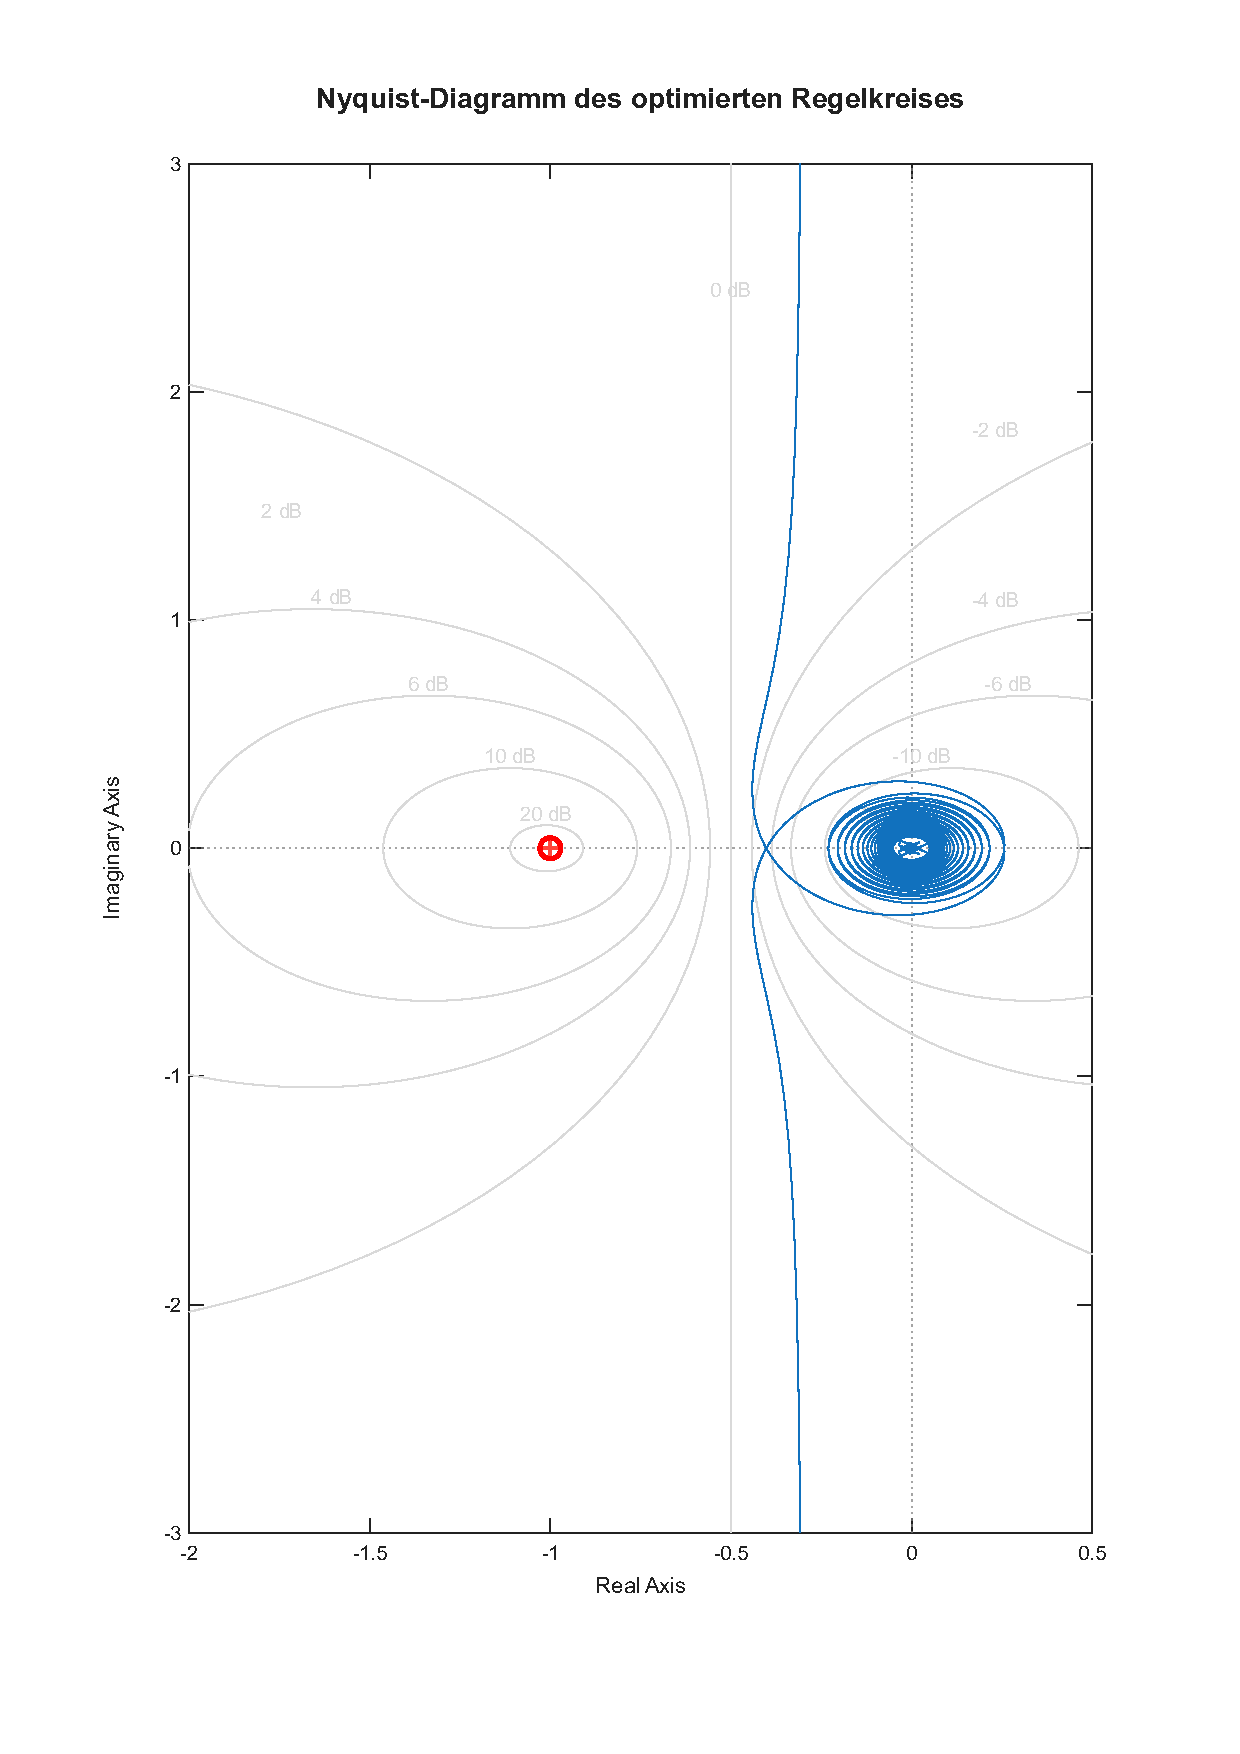
\includegraphics[width=0.7\textwidth]{Abbildungen/nyquist_aufgabe_7A_1.pdf}
    \caption{Nyquist-Diagramm}
    \label{fig:nyquist_7A}
\end{figure}

Wie man anhand des Nyquist-Diagramms in Abbildung~\ref{fig:nyquist_7A} erkennen kann, liegt der kritische Punkt bei $-1 + j0$. Da die Kurve den Punkt $-1$ nicht umschließt, ist der geschlossene Regelkreis stabil und desweiteren Erkennt man das eine große Phasenreserve besteht.
Die Linien häufen sich an einen Punkt und rotieren, im Kreis, dies ist auf die Totzeit zurückzuführen.

\subsection{Aufgabe B -- Regler-Einstellung nach Ziegler-Nichols}
In der zweiten Aufgabe soll die gleiche Strecke geregelt werden, jedoch mit einem PID-Regler, dessen Parameter mit dem heuristischen Verfahren nach Ziegler-Nichols bestimmt werden.

Der Regler soll in die Form

\begin{equation}
G(s)=K\frac{e^{-sT_t}}{1+sT}
\end{equation}

gebracht werden. 


Aus der Strecke:

\begin{equation}
G_S(s)=\frac{1}{2} \cdot \frac{1}{1+0.25s} \cdot e^{-0.3s}
\end{equation}
kann man die Parameter $K$, $T$ und $T_t$ ablesen:

\begin{equation}
K=\frac{1}{2}=0.5
\end{equation}

\begin{equation}
T=\frac{0.5}{2}=0.25\,\mathrm{s}
\end{equation}

\begin{equation}
T_t=0.3\,\mathrm{s}
\end{equation}


Die Ziegler-Nichols-Parameter ergeben sich zu:

\begin{equation}
K_P = 1.2\frac{T}{K T_t} = 1.2\frac{0.25}{0.5 \cdot 0.3} = 2
\end{equation}

\begin{equation}
T_N=2T_t=0.6\,\mathrm{s}
\end{equation}

\begin{equation}
T_V=0.5T_t=0.15\,\mathrm{s}
\end{equation}

Damit lautet die Reglerübertragungsfunktion:

\begin{equation}
G_R(s)= 2 \left( 1+\frac{1}{0.6s} +0.15s \right)
\end{equation}

\subsubsection{Versuchsaufbau und Durchführung}

Als erstes werden die Parameter der Strecke, die daraus resultierenden Strecke und der Regler definiert.

\begin{lstlisting}[language=Matlab, caption={MATLAB-Skript zur Streckendefinition und Stabilitätsanalyse.}]
K=1/2;
T=1/4;
tt=0.3;
Gs = tf(K, [T, 1], 'IoDelay',tt);%Strecke

KP=1.2*T/(K*tt);
TN=2*tt;
TV=0.5*tt;

Gr = pidstd(KP, TN, TV,100);%Regler
\end{lstlisting}

Damit die Sprungantwort analysiert werden kann, bekommt der Regler, wie in der Simulation einen Filter mit $N=100$.

In Simulink wird der Regelkreis aufgebaut, unter der Verwendung der definierten variablen (hierbei ist zu beachten, dass im Regler $I=1/TN=1/(2*0.3)$ ist).

\begin{figure}[H]
    \centering

    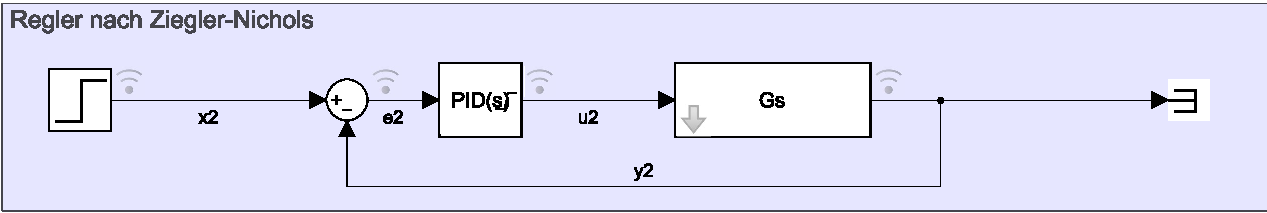
\includegraphics[width=0.9\textwidth]{Abbildungen/regelkreis_7_B1.pdf}
    \caption{Regelkreises mit Ziegler-Nichols-Regler}
    \label{fig:regelkreis_7B1}
\end{figure}

Parameter des Ziegler-Nichols-Reglers: $P = 2$, $I \approx 1.67$ und $D = T_V = 0.15$.
Parameter des Trial-and-Error-Reglers: $P = 1.6$, $I = 2.5$ und $D = 0.06$.

\begin{figure}[H]
    \centering

    % This file was created by matlab2tikz.
%
%The latest updates can be retrieved from
%  http://www.mathworks.com/matlabcentral/fileexchange/22022-matlab2tikz-matlab2tikz
%where you can also make suggestions and rate matlab2tikz.
%
\definecolor{mycolor1}{rgb}{0.00000,0.44700,0.74100}%
\definecolor{mycolor2}{rgb}{0.92900,0.69400,0.12500}%
\definecolor{mycolor3}{rgb}{0.63500,0.07800,0.18400}%
\definecolor{mycolor4}{rgb}{1.00000,0.41200,0.16100}%
\definecolor{mycolor5}{rgb}{0.12941,0.12941,0.12941}%
%
\begin{tikzpicture}

\begin{axis}[%
width=0.951\figurewidth,
height=\figureheight,
at={(0\figurewidth,0\figureheight)},
scale only axis,
xmin=-0.2,
xmax=10.2,
tick align=outside,
xlabel style={font=\color{mycolor5}},
xlabel={Time (seconds)},
ymin=-0.0545790121035998,
ymax=1.1461592541756,
axis background/.style={fill=white},
xmajorgrids,
ymajorgrids,
legend style={at={(0.144,0.935)}, anchor=south west, legend cell align=left, align=left}
]
\addplot [color=mycolor1, line width=2.0pt]
  table[row sep=crcr]{%
0	0\\
0.01	0\\
0.02	0\\
0.03	0\\
0.04	0\\
0.05	0\\
0.06	0\\
0.07	0\\
0.08	0\\
0.09	0\\
0.1	0\\
0.11	0\\
0.12	0\\
0.13	0\\
0.14	0\\
0.15	0\\
0.16	0\\
0.17	0\\
0.18	0\\
0.19	0\\
0.2	0\\
0.21	0\\
0.22	0\\
0.23	0\\
0.24	0\\
0.25	0\\
0.26	0\\
0.27	0\\
0.28	0\\
0.29	0\\
0.3	0\\
0.31	0\\
0.32	0\\
0.33	0\\
0.34	0\\
0.35	0\\
0.36	0\\
0.37	0\\
0.38	0\\
0.39	0\\
0.4	0\\
0.41	0\\
0.42	0\\
0.43	0\\
0.44	0\\
0.45	0\\
0.46	0\\
0.47	0\\
0.48	0\\
0.49	0\\
0.5	0\\
0.51	0\\
0.52	0\\
0.53	0\\
0.54	0\\
0.55	0\\
0.56	0\\
0.57	0\\
0.58	0\\
0.59	0\\
0.6	0\\
0.61	0\\
0.62	0\\
0.63	0\\
0.64	0\\
0.65	0\\
0.66	0\\
0.67	0\\
0.68	0\\
0.69	0\\
0.7	0\\
0.71	0\\
0.72	0\\
0.73	0\\
0.74	0\\
0.75	0\\
0.76	0\\
0.77	0\\
0.78	0\\
0.79	0\\
0.8	0\\
0.81	0\\
0.820000000000001	0\\
0.830000000000001	0\\
0.840000000000001	0\\
0.850000000000001	0\\
0.860000000000001	0\\
0.870000000000001	0\\
0.880000000000001	0\\
0.890000000000001	0\\
0.900000000000001	0\\
0.910000000000001	0\\
0.920000000000001	0\\
0.930000000000001	0\\
0.940000000000001	0\\
0.950000000000001	0\\
0.960000000000001	0\\
0.970000000000001	0\\
0.980000000000001	0\\
0.990000000000001	0\\
0.999999999999994	0\\
1	0\\
1.00706610368157	0\\
1.01413220736314	0\\
1.02274744349539	0\\
1.03274744349539	0\\
1.04274744349539	0\\
1.05274744349539	0\\
1.06274744349539	0\\
1.07274744349539	0\\
1.08274744349539	0\\
1.09274744349539	0\\
1.10274744349539	0\\
1.11274744349539	0\\
1.12274744349539	0\\
1.13274744349539	0\\
1.14274744349539	0\\
1.15274744349539	0\\
1.16274744349539	0\\
1.17274744349539	0\\
1.18274744349539	0\\
1.19274744349539	0\\
1.20274744349539	0\\
1.21274744349539	0\\
1.22274744349539	0\\
1.23274744349539	0\\
1.24274744349539	0\\
1.25274744349539	0\\
1.26274744349539	0\\
1.27274744349539	0\\
1.28274744349539	0\\
1.29274744349539	0\\
1.30274744349539	0.045976526739039\\
1.31274744349539	0.17198149007033\\
1.3225006965157	0.232224622866238\\
1.3325006965157	0.269290295831943\\
1.3425006965157	0.297723636142865\\
1.3525006965157	0.322869813351256\\
1.3625006965157	0.34672523331691\\
1.3725006965157	0.370028375141167\\
1.3825006965157	0.393054258594177\\
1.3925006965157	0.415907077772547\\
1.4025006965157	0.438627992462751\\
1.4125006965157	0.461234835744519\\
1.4225006965157	0.483736743901422\\
1.4325006965157	0.506139549213569\\
1.4425006965157	0.52844777025078\\
1.4525006965157	0.550665348756964\\
1.4625006965157	0.57279592471353\\
1.4725006965157	0.594842941155847\\
1.4825006965157	0.61680968614478\\
1.4925006965157	0.638699311458444\\
1.5025006965157	0.660514842582491\\
1.5125006965157	0.682259185373591\\
1.5225006965157	0.703935131380554\\
1.5325006965157	0.725545362558598\\
1.5425006965157	0.747092455652101\\
1.5525006965157	0.768578886351481\\
1.5625006965157	0.790007033267177\\
1.5725006965157	0.811379181740491\\
1.5825006965157	0.832697527502289\\
1.5925006965157	0.853964180187262\\
1.6025006965157	0.874116368225063\\
1.6125006965157	0.87739444062503\\
1.6225006965157	0.877550060023196\\
1.6325006965157	0.880945674949175\\
1.6425006965157	0.886930627737664\\
1.6525006965157	0.894208425724866\\
1.6625006965157	0.901880607749053\\
1.6725006965157	0.909463103369961\\
1.6825006965157	0.916723162813402\\
1.6925006965157	0.923556871902859\\
1.7025006965157	0.929921048582164\\
1.7125006965157	0.935799694250152\\
1.7225006965157	0.941188522408776\\
1.7325006965157	0.946088116094942\\
1.7425006965157	0.95050098917805\\
1.7525006965157	0.954430352716008\\
1.7625006965157	0.957879607614064\\
1.7725006965157	0.96085214088586\\
1.7825006965157	0.963351246919433\\
1.7925006965157	0.965380099533735\\
1.8025006965157	0.9669417443891\\
1.8125006965157	0.968039099402968\\
1.8225006965157	0.968674958207471\\
1.8325006965157	0.968851994671798\\
1.8425006965157	0.968572767710063\\
1.8525006965157	0.967839726072492\\
1.8625006965157	0.966655213006504\\
1.8725006965157	0.965021470748477\\
1.8825006965157	0.962940644835904\\
1.8925006965157	0.96041478824072\\
1.9025006965157	0.957535507343841\\
1.9125006965157	0.955744360711574\\
1.9225006965157	0.955610668199473\\
1.9325006965157	0.956004450706358\\
1.9425006965157	0.956163002080479\\
1.9525006965157	0.955917298487664\\
1.9625006965157	0.955336006064356\\
1.9725006965157	0.954530750963973\\
1.9825006965157	0.953591118623185\\
1.9925006965157	0.952576694340924\\
2.0025006965157	0.95152500246467\\
2.0125006965157	0.950460271901534\\
2.0225006965157	0.949399494234172\\
2.0325006965157	0.948355948262503\\
2.0425006965157	0.947341068113859\\
2.0525006965157	0.946365376834665\\
2.0625006965157	0.945438934861871\\
2.0725006965157	0.944571549969103\\
2.0825006965157	0.94377287434361\\
2.0925006965157	0.943052449737043\\
2.1025006965157	0.942419729213902\\
2.1125006965157	0.941884088493381\\
2.12250069651569	0.941454832682746\\
2.13250069651569	0.941141200947061\\
2.14250069651569	0.940952370218469\\
2.15250069651569	0.940897458419777\\
2.16250069651569	0.940985527406596\\
2.17250069651569	0.94122558571722\\
2.18250069651569	0.941626591170741\\
2.19250069651569	0.942197453333488\\
2.20250069651569	0.94293935889934\\
2.21250069651569	0.943728542486283\\
2.22250069651569	0.944371206678039\\
2.23250069651569	0.944834680691723\\
2.24250069651569	0.945228347444686\\
2.25250069651569	0.945653611915153\\
2.26250069651569	0.946157218686349\\
2.27250069651569	0.946747478217163\\
2.28250069651569	0.947416291240615\\
2.29250069651569	0.948151995625076\\
2.30250069651569	0.948944331361061\\
2.31250069651569	0.949785401634814\\
2.32250069651569	0.950669210037992\\
2.33250069651569	0.951590952632379\\
2.34250069651569	0.952546452616319\\
2.35250069651569	0.953531793714977\\
2.36250069651569	0.954543107470297\\
2.37250069651569	0.955576458515744\\
2.38250069651569	0.956627786023791\\
2.39250069651569	0.957692875246734\\
2.40250069651569	0.958767344411823\\
2.41250069651569	0.959846639156432\\
2.42250069651569	0.960926030545254\\
2.43250069651569	0.962000614733385\\
2.44250069651569	0.963065313354478\\
2.45250069651569	0.964114874206398\\
2.46250069651569	0.965143872040352\\
2.47250069651569	0.966146709367626\\
2.48250069651569	0.967117617247223\\
2.49250069651569	0.968050656039753\\
2.50250069651569	0.9689403735799\\
2.51250069651569	0.96979264125636\\
2.52250069651569	0.970632509366025\\
2.53250069651569	0.971485206733013\\
2.54250069651569	0.972355141530744\\
2.55250069651569	0.973229970440752\\
2.56250069651569	0.974094792058557\\
2.57250069651569	0.974939480229114\\
2.58250069651569	0.975759153258169\\
2.59250069651568	0.976552235576438\\
2.60250069651568	0.977318637349027\\
2.61250069651568	0.978058695675337\\
2.62250069651568	0.978772732626215\\
2.63250069651568	0.979460949987933\\
2.64250069651568	0.980123460648534\\
2.65250069651568	0.980760353777007\\
2.66250069651568	0.98137175350712\\
2.67250069651568	0.981957861287912\\
2.68250069651568	0.982518983558834\\
2.69250069651568	0.983055549126594\\
2.70250069651568	0.983568120149751\\
2.71250069651568	0.984057399447254\\
2.72250069651568	0.984524235802028\\
2.73250069651568	0.984969628212546\\
2.74250069651568	0.985394729607831\\
2.75250069651568	0.985800850293955\\
2.76250069651568	0.986189461267294\\
2.77250069651568	0.986562197461244\\
2.78250069651568	0.986920860958734\\
2.79250069651568	0.987267424186114\\
2.80250069651568	0.987603976791092\\
2.81250069651568	0.987931732729497\\
2.82250069651568	0.988249202826056\\
2.83250069651568	0.988552413282814\\
2.84250069651568	0.988837869154007\\
2.85250069651568	0.989104811130687\\
2.86250069651568	0.989354850589151\\
2.87250069651568	0.98959043388465\\
2.88250069651568	0.989813744734469\\
2.89250069651568	0.990026359524929\\
2.90250069651568	0.990229336912809\\
2.91250069651568	0.990423423070077\\
2.92250069651568	0.990609219240532\\
2.93250069651568	0.990787278028006\\
2.94250069651568	0.990958144081113\\
2.95250069651568	0.991122363115869\\
2.96250069651568	0.99128047691369\\
2.97250069651568	0.991433014038047\\
2.98250069651568	0.991580480529\\
2.99250069651568	0.99172335189896\\
3.00250069651568	0.991862066489594\\
3.01250069651568	0.991997019853553\\
3.02250069651568	0.99212855979477\\
3.03250069651568	0.992256981785812\\
3.04250069651568	0.992382524575948\\
3.05250069651568	0.992505365876982\\
3.06250069651567	0.992625618062339\\
3.07250069651567	0.992743323844176\\
3.08250069651567	0.992858451909866\\
3.09250069651567	0.992970892508283\\
3.10250069651567	0.993080457802965\\
3.11250069651567	0.993186968486778\\
3.12250069651567	0.993290512198557\\
3.13250069651567	0.993391664982705\\
3.14250069651567	0.993491343706774\\
3.15250069651567	0.993590381654533\\
3.16250069651567	0.993689233231202\\
3.17250069651567	0.993787981923537\\
3.18250069651567	0.993886512550412\\
3.19250069651567	0.993984671072353\\
3.20250069651567	0.99408234477416\\
3.21250069651567	0.994179477009221\\
3.22250069651567	0.994276051332659\\
3.23250069651567	0.994372070068489\\
3.24250069651567	0.994467538197613\\
3.25250069651567	0.994562454475691\\
3.26250069651567	0.99465680808565\\
3.27250069651567	0.994750578570291\\
3.28250069651567	0.994843737357309\\
3.29250069651567	0.994936249898098\\
3.30250069651567	0.995028077958895\\
3.31250069651567	0.995119181898619\\
3.32250069651567	0.995209522907121\\
3.33250069651567	0.995299065228928\\
3.34250069651567	0.995387778407826\\
3.35250069651567	0.995475639582485\\
3.36250069651567	0.995562635854877\\
3.37250069651567	0.995648766745763\\
3.38250069651567	0.995734046746304\\
3.39250069651567	0.99581850797139\\
3.40250069651567	0.995902202505381\\
3.41250069651567	0.995985196963502\\
3.42250069651567	0.996067543242251\\
3.43250069651567	0.996149229980435\\
3.44250069651567	0.996230157333947\\
3.45250069651567	0.996310167376325\\
3.46250069651567	0.996389106134619\\
3.47250069651567	0.996466868355141\\
3.48250069651567	0.996543404366636\\
3.49250069651567	0.996618702048265\\
3.50250069651567	0.996692764742082\\
3.51250069651567	0.99676559661714\\
3.52250069651567	0.996837196920311\\
3.53250069651566	0.996907559969444\\
3.54250069651566	0.996976677450121\\
3.55250069651566	0.997044540882312\\
3.56250069651566	0.997111143397107\\
3.57250069651566	0.997176480712807\\
3.58250069651566	0.997240551493317\\
3.59250069651566	0.997303357312496\\
3.60250069651566	0.997364902393198\\
3.61250069651566	0.997425193221567\\
3.62250069651566	0.997484238085785\\
3.63250069651566	0.997542046557483\\
3.64250069651566	0.997598628918524\\
3.65250069651566	0.997653995529361\\
3.66250069651566	0.997708156133427\\
3.67250069651566	0.997761119092112\\
3.68250069651566	0.997812890545592\\
3.69250069651566	0.997863473495505\\
3.70250069651566	0.997912866841378\\
3.71250069651566	0.997961065051023\\
3.72250069651566	0.998008060631812\\
3.73250069651566	0.998053851085464\\
3.74250069651566	0.99809844734603\\
3.75250069651566	0.998141877042019\\
3.76250069651566	0.998184179502837\\
3.77250069651566	0.998225396461688\\
3.78250069651566	0.998265564735012\\
3.79250069651566	0.998304713828475\\
3.80250069651566	0.998342867402657\\
3.81250069651566	0.998380046089081\\
3.82250069651566	0.998416269838361\\
3.83250069651566	0.998451559183362\\
3.84250069651566	0.998485935577394\\
3.85250069651566	0.998519421210897\\
3.86250069651566	0.998552038648366\\
3.87250069651566	0.998583810480547\\
3.88250069651566	0.998614759066571\\
3.89250069651566	0.998644906373265\\
3.90250069651566	0.998674273893024\\
3.91250069651566	0.998702882618495\\
3.92250069651566	0.99873075305794\\
3.93250069651566	0.998757905282048\\
3.94250069651566	0.998784358998338\\
3.95250069651566	0.998810133652647\\
3.96250069651566	0.99883524855904\\
3.97250069651566	0.998859723060301\\
3.98250069651566	0.998883576721499\\
3.99250069651566	0.998906829559191\\
4.00250069651566	0.99892950230581\\
4.01250069651566	0.998951616649603\\
4.02250069651565	0.998973195194152\\
4.03250069651565	0.998994260733321\\
4.04250069651565	0.999014834786626\\
4.05250069651565	0.999034936094751\\
4.06250069651565	0.99905458005532\\
4.07250069651565	0.999073779421433\\
4.08250069651565	0.999092545682332\\
4.09250069651565	0.999110890270525\\
4.10250069651565	0.999128825128567\\
4.11250069651565	0.999146362681222\\
4.12250069651565	0.999163515508775\\
4.13250069651565	0.999180295994381\\
4.14250069651565	0.999196716084013\\
4.15250069651565	0.999212787180352\\
4.16250069651565	0.999228520134033\\
4.17250069651565	0.999243925285219\\
4.18250069651565	0.99925901252041\\
4.19250069651565	0.999273791325267\\
4.20250069651565	0.999288270826086\\
4.21250069651565	0.99930245981895\\
4.22250069651565	0.999316366787936\\
4.23250069651565	0.99932999991402\\
4.24250069651565	0.999343367075648\\
4.25250069651565	0.9993564758412\\
4.26250069651565	0.999369333452935\\
4.27250069651565	0.9993819468016\\
4.28250069651565	0.999394322390609\\
4.29250069651565	0.999406466288552\\
4.30250069651565	0.99941838406895\\
4.31250069651565	0.999430080741479\\
4.32250069651565	0.999441560701946\\
4.33250069651565	0.9994528277645\\
4.34250069651565	0.999463885337528\\
4.35250069651565	0.999474736720106\\
4.36250069651565	0.999485385387056\\
4.37250069651565	0.999495835116182\\
4.38250069651565	0.99950608991609\\
4.39250069651565	0.999516153835521\\
4.40250069651565	0.999526030775603\\
4.41250069651565	0.999535724382185\\
4.42250069651565	0.999545238027715\\
4.43250069651565	0.999554574850358\\
4.44250069651565	0.999563737811381\\
4.45250069651565	0.999572729744966\\
4.46250069651565	0.999581553390832\\
4.47250069651565	0.999590211410764\\
4.48250069651565	0.999598706394388\\
4.49250069651564	0.999607040859583\\
4.50250069651564	0.999615217251316\\
4.51250069651564	0.999623237940968\\
4.52250069651564	0.999631105227041\\
4.53250069651564	0.99963882133752\\
4.54250069651564	0.999646388433965\\
4.55250069651564	0.999653808617391\\
4.56250069651564	0.999661083936125\\
4.57250069651564	0.999668216395919\\
4.58250069651564	0.99967520797269\\
4.59250069651564	0.999682060628373\\
4.60250069651564	0.999688776330375\\
4.61250069651564	0.999695357074709\\
4.62250069651564	0.99970180491039\\
4.63250069651564	0.999708121956898\\
4.64250069651564	0.999714310401594\\
4.65250069651564	0.99972037246855\\
4.66250069651564	0.999726310366505\\
4.67250069651564	0.999732126239027\\
4.68250069651564	0.99973782213974\\
4.69250069651564	0.999743400039443\\
4.70250069651564	0.999748861854403\\
4.71250069651564	0.999754209478278\\
4.72250069651564	0.999759444804757\\
4.73250069651564	0.999764569737046\\
4.74250069651564	0.999769586187073\\
4.75250069651564	0.999774496069683\\
4.76250069651564	0.999779301296119\\
4.77250069651564	0.999784003769154\\
4.78250069651564	0.999788605380419\\
4.79250069651564	0.99979310800955\\
4.80250069651564	0.999797513524457\\
4.81250069651564	0.999801823782083\\
4.82250069651564	0.999806040629231\\
4.83250069651564	0.999810165903185\\
4.84250069651564	0.999814201432009\\
4.85250069651564	0.99981814903441\\
4.86250069651564	0.999822010519109\\
4.87250069651564	0.999825787683607\\
4.88250069651564	0.999829482312245\\
4.89250069651564	0.999833096173413\\
4.90250069651564	0.999836631015721\\
4.91250069651564	0.99984008856301\\
4.92250069651564	0.999843470508272\\
4.93250069651564	0.999846778507353\\
4.94250069651564	0.999850014174433\\
4.95250069651564	0.999853179081832\\
4.96250069651563	0.999856274765296\\
4.97250069651563	0.999859302733118\\
4.98250069651563	0.999862264475142\\
4.99250069651563	0.999865161467956\\
5.00250069651563	0.999867995174926\\
5.01250069651563	0.9998707670424\\
5.02250069651563	0.999873478494611\\
5.03250069651563	0.999876130929431\\
5.04250069651563	0.99987872571593\\
5.05250069651563	0.999881264193648\\
5.06250069651563	0.999883747672936\\
5.07250069651563	0.999886177435702\\
5.08250069651563	0.9998885547361\\
5.09250069651563	0.999890880800971\\
5.10250069651563	0.999893156830006\\
5.11250069651563	0.99989538399571\\
5.12250069651563	0.999897563443252\\
5.13250069651563	0.999899696290271\\
5.14250069651563	0.999901783626722\\
5.15250069651563	0.999903826514775\\
5.16250069651563	0.999905825988819\\
5.17250069651563	0.999907783055594\\
5.18250069651563	0.999909698694495\\
5.19250069651563	0.99991157385808\\
5.20250069651563	0.999913409472842\\
5.21250069651563	0.999915206440295\\
5.22250069651563	0.999916965638417\\
5.23250069651563	0.999918687923399\\
5.24250069651563	0.999920374131456\\
5.25250069651563	0.999922025080277\\
5.26250069651563	0.999923641569606\\
5.27250069651563	0.999925224380803\\
5.28250069651563	0.999926774275673\\
5.29250069651563	0.999928291995234\\
5.30250069651563	0.999929778259041\\
5.31250069651563	0.99993123376534\\
5.32250069651563	0.999932659191928\\
5.33250069651563	0.999934055197338\\
5.34250069651563	0.999935422422018\\
5.35250069651563	0.999936761489299\\
5.36250069651563	0.999938073006091\\
5.37250069651563	0.999939357563402\\
5.38250069651563	0.999940615736744\\
5.39250069651563	0.999941848086531\\
5.40250069651563	0.999943055158485\\
5.41250069651563	0.999944237484102\\
5.42250069651563	0.999945395581139\\
5.43250069651562	0.999946529954142\\
5.44250069651562	0.999947641094978\\
5.45250069651562	0.999948729483373\\
5.46250069651562	0.999949795587444\\
5.47250069651562	0.999950839864204\\
5.48250069651562	0.999951862760043\\
5.49250069651562	0.999952864711164\\
5.50250069651562	0.999953846143965\\
5.51250069651562	0.999954807475347\\
5.52250069651562	0.999955749112928\\
5.53250069651562	0.99995667145516\\
5.54250069651562	0.99995757489136\\
5.55250069651562	0.999958459801713\\
5.56250069651562	0.999959326557333\\
5.57250069651562	0.999960175520482\\
5.58250069651562	0.999961007044976\\
5.59250069651562	0.999961821476718\\
5.60250069651562	0.999962619154264\\
5.61250069651562	0.999963400409303\\
5.62250069651562	0.999964165566994\\
5.63250069651562	0.999964914946178\\
5.64250069651562	0.999965648859505\\
5.65250069651562	0.999966367613524\\
5.66250069651562	0.999967071508798\\
5.67250069651562	0.999967760840034\\
5.68250069651562	0.99996843589624\\
5.69250069651562	0.999969096960888\\
5.70250069651562	0.999969744312086\\
5.71250069651562	0.999970378222725\\
5.72250069651562	0.999970998960625\\
5.73250069651562	0.999971606788651\\
5.74250069651562	0.999972201964828\\
5.75250069651562	0.999972784742425\\
5.76250069651562	0.999973355370047\\
5.77250069651562	0.999973914091703\\
5.78250069651562	0.999974461146877\\
5.79250069651562	0.99997499677059\\
5.80250069651562	0.999975521193467\\
5.81250069651562	0.999976034641809\\
5.82250069651562	0.999976537337671\\
5.83250069651562	0.999977029498962\\
5.84250069651562	0.999977511339559\\
5.85250069651562	0.999977983069435\\
5.86250069651562	0.999978444894792\\
5.87250069651562	0.99997889701818\\
5.88250069651562	0.999979339638577\\
5.89250069651562	0.999979772951435\\
5.90250069651561	0.999980197148695\\
5.91250069651561	0.999980612418781\\
5.92250069651561	0.999981018946613\\
5.93250069651561	0.999981416913624\\
5.94250069651561	0.999981806497803\\
5.95250069651561	0.999982187873747\\
5.96250069651561	0.999982561212726\\
5.97250069651561	0.999982926682732\\
5.98250069651561	0.999983284448542\\
5.99250069651561	0.999983634671756\\
6.00250069651561	0.999983977510843\\
6.01250069651561	0.999984313121185\\
6.02250069651561	0.99998464165511\\
6.03250069651561	0.999984963261941\\
6.04250069651561	0.99998527808803\\
6.05250069651561	0.99998558627681\\
6.06250069651561	0.999985887968836\\
6.07250069651561	0.999986183301834\\
6.08250069651561	0.999986472410749\\
6.09250069651561	0.999986755427794\\
6.10250069651561	0.9999870324825\\
6.11250069651561	0.999987303701763\\
6.12250069651561	0.999987569209894\\
6.13250069651561	0.999987829128654\\
6.14250069651561	0.999988083577302\\
6.15250069651561	0.999988332672623\\
6.16250069651561	0.999988576528959\\
6.17250069651561	0.999988815258234\\
6.18250069651561	0.999989048969986\\
6.19250069651561	0.9999892777714\\
6.20250069651561	0.999989501767347\\
6.21250069651561	0.999989721060435\\
6.22250069651561	0.999989935751054\\
6.23250069651561	0.999990145937428\\
6.24250069651561	0.999990351715661\\
6.25250069651561	0.999990553179776\\
6.26250069651561	0.999990750421765\\
6.27250069651561	0.999990943531616\\
6.28250069651561	0.999991132597361\\
6.29250069651561	0.999991317705106\\
6.30250069651561	0.999991498939077\\
6.31250069651561	0.999991676381654\\
6.32250069651561	0.999991850113412\\
6.33250069651561	0.999992020213158\\
6.34250069651561	0.999992186757972\\
6.35250069651561	0.999992349823242\\
6.36250069651561	0.999992509482701\\
6.3725006965156	0.999992665808462\\
6.3825006965156	0.999992818871055\\
6.3925006965156	0.999992968739456\\
6.4025006965156	0.999993115481125\\
6.4125006965156	0.999993259162037\\
6.4225006965156	0.999993399846708\\
6.4325006965156	0.999993537598237\\
6.4425006965156	0.999993672478326\\
6.4525006965156	0.999993804547322\\
6.4625006965156	0.999993933864243\\
6.4725006965156	0.999994060486812\\
6.4825006965156	0.999994184471494\\
6.4925006965156	0.999994305873521\\
6.5025006965156	0.999994424746931\\
6.5125006965156	0.999994541144587\\
6.5225006965156	0.999994655118215\\
6.5325006965156	0.999994766718421\\
6.5425006965156	0.999994875994719\\
6.5525006965156	0.999994982995559\\
6.5625006965156	0.999995087768345\\
6.5725006965156	0.999995190359464\\
6.5825006965156	0.999995290814311\\
6.5925006965156	0.999995389177308\\
6.6025006965156	0.99999548549193\\
6.6125006965156	0.999995579800727\\
6.6225006965156	0.999995672145345\\
6.6325006965156	0.999995762566549\\
6.6425006965156	0.999995851104239\\
6.6525006965156	0.999995937797474\\
6.6625006965156	0.999996022684491\\
6.6725006965156	0.99999610580272\\
6.6825006965156	0.999996187188808\\
6.6925006965156	0.999996266878634\\
6.7025006965156	0.999996344907326\\
6.7125006965156	0.999996421309282\\
6.7225006965156	0.999996496118183\\
6.7325006965156	0.999996569367012\\
6.7425006965156	0.999996641088069\\
6.7525006965156	0.999996711312989\\
6.7625006965156	0.999996780072752\\
6.7725006965156	0.999996847397703\\
6.7825006965156	0.999996913317561\\
6.7925006965156	0.999996977861434\\
6.8025006965156	0.999997041057832\\
6.8125006965156	0.999997102934681\\
6.8225006965156	0.999997163519332\\
6.83250069651559	0.999997222838574\\
6.84250069651559	0.999997280918648\\
6.85250069651559	0.999997337785258\\
6.86250069651559	0.999997393463582\\
6.87250069651559	0.999997447978282\\
6.88250069651559	0.999997501353517\\
6.89250069651559	0.999997553612954\\
6.90250069651559	0.999997604779775\\
6.91250069651559	0.999997654876688\\
6.92250069651559	0.999997703925938\\
6.93250069651559	0.999997751949318\\
6.94250069651559	0.999997798968172\\
6.95250069651559	0.999997845003412\\
6.96250069651559	0.999997890075519\\
6.97250069651559	0.99999793420456\\
6.98250069651559	0.999997977410188\\
6.99250069651559	0.999998019711656\\
7.00250069651559	0.999998061127824\\
7.01250069651559	0.999998101677164\\
7.02250069651559	0.999998141377771\\
7.03250069651559	0.999998180247367\\
7.04250069651559	0.999998218303314\\
7.05250069651559	0.999998255562612\\
7.06250069651559	0.999998292041916\\
7.07250069651559	0.999998327757536\\
7.08250069651559	0.999998362725445\\
7.09250069651559	0.999998396961287\\
7.10250069651559	0.999998430480384\\
7.11250069651559	0.99999846329774\\
7.12250069651559	0.999998495428051\\
7.13250069651559	0.999998526885707\\
7.14250069651559	0.9999985576848\\
7.15250069651559	0.999998587839132\\
7.16250069651559	0.999998617362215\\
7.17250069651559	0.999998646267285\\
7.18250069651559	0.999998674567299\\
7.19250069651559	0.999998702274946\\
7.20250069651559	0.99999872940265\\
7.21250069651559	0.999998755962577\\
7.22250069651559	0.999998781966637\\
7.23250069651559	0.999998807426495\\
7.24250069651559	0.999998832353568\\
7.25250069651559	0.999998856759036\\
7.26250069651559	0.999998880653846\\
7.27250069651559	0.999998904048713\\
7.28250069651559	0.999998926954129\\
7.29250069651559	0.999998949380366\\
7.30250069651558	0.999998971337478\\
7.31250069651558	0.999998992835311\\
7.32250069651558	0.999999013883501\\
7.33250069651558	0.999999034491483\\
7.34250069651558	0.999999054668493\\
7.35250069651558	0.999999074423572\\
7.36250069651558	0.99999909376557\\
7.37250069651558	0.999999112703153\\
7.38250069651558	0.999999131244802\\
7.39250069651558	0.99999914939882\\
7.40250069651558	0.999999167173335\\
7.41250069651558	0.999999184576304\\
7.42250069651558	0.999999201615515\\
7.43250069651558	0.999999218298592\\
7.44250069651558	0.999999234632999\\
7.45250069651558	0.999999250626041\\
7.46250069651558	0.999999266284871\\
7.47250069651558	0.999999281616488\\
7.48250069651558	0.999999296627745\\
7.49250069651558	0.999999311325352\\
7.50250069651558	0.999999325715873\\
7.51250069651558	0.999999339805738\\
7.52250069651558	0.999999353601239\\
7.53250069651558	0.999999367108535\\
7.54250069651558	0.999999380333656\\
7.55250069651558	0.999999393282505\\
7.56250069651558	0.99999940596086\\
7.57250069651558	0.999999418374378\\
7.58250069651558	0.999999430528595\\
7.59250069651558	0.999999442428933\\
7.60250069651558	0.999999454080698\\
7.61250069651558	0.999999465489084\\
7.62250069651558	0.999999476659179\\
7.63250069651558	0.99999948759596\\
7.64250069651558	0.999999498304301\\
7.65250069651558	0.999999508788974\\
7.66250069651558	0.999999519054652\\
7.67250069651558	0.999999529105906\\
7.68250069651558	0.999999538947215\\
7.69250069651558	0.999999548582962\\
7.70250069651558	0.999999558017439\\
7.71250069651558	0.999999567254847\\
7.72250069651558	0.9999995762993\\
7.73250069651558	0.999999585154825\\
7.74250069651558	0.999999593825366\\
7.75250069651558	0.999999602314783\\
7.76250069651558	0.999999610626856\\
7.77250069651557	0.999999618765285\\
7.78250069651557	0.999999626733695\\
7.79250069651557	0.999999634535633\\
7.80250069651557	0.999999642174572\\
7.81250069651557	0.999999649653914\\
7.82250069651557	0.999999656976989\\
7.83250069651557	0.999999664147058\\
7.84250069651557	0.999999671167313\\
7.85250069651557	0.99999967804088\\
7.86250069651557	0.99999968477082\\
7.87250069651557	0.99999969136013\\
7.88250069651557	0.999999697811745\\
7.89250069651557	0.999999704128539\\
7.90250069651557	0.999999710313324\\
7.91250069651557	0.999999716368856\\
7.92250069651557	0.999999722297833\\
7.93250069651557	0.999999728102896\\
7.94250069651557	0.999999733786631\\
7.95250069651557	0.999999739351571\\
7.96250069651557	0.999999744800195\\
7.97250069651557	0.999999750134933\\
7.98250069651557	0.999999755358162\\
7.99250069651557	0.99999976047221\\
8.00250069651557	0.999999765479357\\
8.01250069651557	0.999999770381835\\
8.02250069651557	0.99999977518183\\
8.03250069651557	0.999999779881482\\
8.04250069651557	0.999999784482887\\
8.05250069651557	0.999999788988098\\
8.06250069651557	0.999999793399124\\
8.07250069651557	0.999999797717932\\
8.08250069651557	0.999999801946449\\
8.09250069651557	0.999999806086562\\
8.10250069651557	0.999999810140118\\
8.11250069651557	0.999999814108925\\
8.12250069651557	0.999999817994756\\
8.13250069651557	0.999999821799343\\
8.14250069651557	0.999999825524386\\
8.15250069651557	0.999999829171546\\
8.16250069651557	0.999999832742452\\
8.17250069651557	0.999999836238698\\
8.18250069651557	0.999999839661845\\
8.19250069651557	0.999999843013421\\
8.20250069651557	0.999999846294922\\
8.21250069651557	0.999999849507814\\
8.22250069651557	0.999999852653532\\
8.23250069651557	0.999999855733479\\
8.24250069651556	0.999999858749032\\
8.25250069651556	0.999999861701536\\
8.26250069651556	0.999999864592311\\
8.27250069651556	0.999999867422648\\
8.28250069651556	0.999999870193811\\
8.29250069651556	0.999999872907037\\
8.30250069651556	0.999999875563538\\
8.31250069651556	0.9999998781645\\
8.32250069651556	0.999999880711086\\
8.33250069651556	0.999999883204432\\
8.34250069651556	0.999999885645652\\
8.35250069651556	0.999999888035837\\
8.36250069651556	0.999999890376054\\
8.37250069651556	0.999999892667348\\
8.38250069651556	0.999999894910742\\
8.39250069651556	0.999999897107239\\
8.40250069651556	0.999999899257819\\
8.41250069651556	0.999999901363443\\
8.42250069651556	0.999999903425052\\
8.43250069651556	0.999999905443564\\
8.44250069651556	0.999999907419884\\
8.45250069651556	0.999999909354891\\
8.46250069651556	0.999999911249452\\
8.47250069651556	0.999999913104411\\
8.48250069651556	0.999999914920596\\
8.49250069651556	0.99999991669882\\
8.50250069651556	0.999999918439875\\
8.51250069651556	0.999999920144539\\
8.52250069651556	0.999999921813574\\
8.53250069651556	0.999999923447723\\
8.54250069651556	0.999999925047716\\
8.55250069651556	0.999999926614269\\
8.56250069651556	0.999999928148079\\
8.57250069651556	0.999999929649832\\
8.58250069651556	0.999999931120198\\
8.59250069651556	0.999999932559833\\
8.60250069651556	0.999999933969379\\
8.61250069651556	0.999999935349466\\
8.62250069651556	0.99999993670071\\
8.63250069651556	0.999999938023713\\
8.64250069651556	0.999999939319066\\
8.65250069651556	0.999999940587347\\
8.66250069651556	0.999999941829121\\
8.67250069651556	0.999999943044943\\
8.68250069651556	0.999999944235356\\
8.69250069651556	0.99999994540089\\
8.70250069651556	0.999999946542065\\
8.71250069651555	0.999999947659391\\
8.72250069651555	0.999999948753365\\
8.73250069651555	0.999999949824477\\
8.74250069651555	0.999999950873203\\
8.75250069651555	0.999999951900012\\
8.76250069651555	0.999999952905361\\
8.77250069651555	0.9999999538897\\
8.78250069651555	0.999999954853467\\
8.79250069651555	0.999999955797091\\
8.80250069651555	0.999999956720995\\
8.81250069651555	0.99999995762559\\
8.82250069651555	0.999999958511279\\
8.83250069651555	0.999999959378458\\
8.84250069651555	0.999999960227513\\
8.85250069651555	0.999999961058823\\
8.86250069651555	0.999999961872759\\
8.87250069651555	0.999999962669684\\
8.88250069651555	0.999999963449953\\
8.89250069651555	0.999999964213915\\
8.90250069651555	0.99999996496191\\
8.91250069651555	0.999999965694272\\
8.92250069651555	0.999999966411327\\
8.93250069651555	0.999999967113395\\
8.94250069651555	0.99999996780079\\
8.95250069651555	0.999999968473817\\
8.96250069651555	0.999999969132778\\
8.97250069651555	0.999999969777966\\
8.98250069651555	0.999999970409669\\
8.99250069651555	0.999999971028169\\
9.00250069651555	0.999999971633741\\
9.01250069651555	0.999999972226656\\
9.02250069651555	0.999999972807179\\
9.03250069651555	0.999999973375567\\
9.04250069651555	0.999999973932076\\
9.05250069651555	0.999999974476952\\
9.06250069651555	0.999999975010439\\
9.07250069651555	0.999999975532776\\
9.08250069651555	0.999999976044195\\
9.09250069651555	0.999999976544924\\
9.10250069651555	0.999999977035186\\
9.11250069651555	0.999999977515201\\
9.12250069651555	0.999999977985183\\
9.13250069651555	0.999999978445341\\
9.14250069651555	0.99999997889588\\
9.15250069651555	0.999999979337002\\
9.16250069651555	0.999999979768904\\
9.17250069651555	0.999999980191778\\
9.18250069651554	0.999999980605812\\
9.19250069651554	0.999999981011192\\
9.20250069651554	0.999999981408099\\
9.21250069651554	0.999999981796709\\
9.22250069651554	0.999999982177196\\
9.23250069651554	0.999999982549729\\
9.24250069651554	0.999999982914476\\
9.25250069651554	0.999999983271598\\
9.26250069651554	0.999999983621256\\
9.27250069651554	0.999999983963605\\
9.28250069651554	0.999999984298797\\
9.29250069651554	0.999999984626983\\
9.30250069651554	0.99999998494831\\
9.31250069651554	0.999999985262919\\
9.32250069651554	0.999999985570952\\
9.33250069651554	0.999999985872547\\
9.34250069651554	0.999999986167837\\
9.35250069651554	0.999999986456955\\
9.36250069651554	0.99999998674003\\
9.37250069651554	0.999999987017187\\
9.38250069651554	0.999999987288552\\
9.39250069651554	0.999999987554243\\
9.40250069651554	0.999999987814382\\
9.41250069651554	0.999999988069083\\
9.42250069651554	0.999999988318459\\
9.43250069651554	0.999999988562624\\
9.44250069651554	0.999999988801684\\
9.45250069651554	0.999999989035748\\
9.46250069651554	0.999999989264919\\
9.47250069651554	0.9999999894893\\
9.48250069651554	0.999999989708991\\
9.49250069651554	0.99999998992409\\
9.50250069651554	0.999999990134693\\
9.51250069651554	0.999999990340894\\
9.52250069651554	0.999999990542785\\
9.53250069651554	0.999999990740455\\
9.54250069651554	0.999999990933995\\
9.55250069651554	0.999999991123488\\
9.56250069651554	0.999999991309021\\
9.57250069651554	0.999999991490676\\
9.58250069651554	0.999999991668534\\
9.59250069651554	0.999999991842675\\
9.60250069651554	0.999999992013176\\
9.61250069651554	0.999999992180113\\
9.62250069651554	0.999999992343561\\
9.63250069651554	0.999999992503592\\
9.64250069651554	0.999999992660278\\
9.65250069651553	0.99999999281369\\
9.66250069651553	0.999999992963895\\
9.67250069651553	0.99999999311096\\
9.68250069651553	0.999999993254952\\
9.69250069651553	0.999999993395934\\
9.70250069651553	0.999999993533969\\
9.71250069651553	0.999999993669119\\
9.72250069651553	0.999999993801444\\
9.73250069651553	0.999999993931004\\
9.74250069651553	0.999999994057855\\
9.75250069651553	0.999999994182056\\
9.76250069651553	0.99999999430366\\
9.77250069651553	0.999999994422722\\
9.78250069651553	0.999999994539296\\
9.79250069651553	0.999999994653434\\
9.80250069651553	0.999999994765186\\
9.81250069651553	0.999999994874602\\
9.82250069651553	0.999999994981731\\
9.83250069651553	0.999999995086621\\
9.84250069651553	0.999999995189319\\
9.85250069651553	0.99999999528987\\
9.86250069651553	0.999999995388319\\
9.87250069651553	0.999999995484711\\
9.88250069651553	0.999999995579088\\
9.89250069651553	0.999999995671493\\
9.90250069651553	0.999999995761966\\
9.91250069651553	0.999999995850548\\
9.92250069651553	0.999999995937279\\
9.93250069651553	0.999999996022196\\
9.94250069651553	0.999999996105339\\
9.95250069651553	0.999999996186745\\
9.96250069651553	0.999999996266448\\
9.97250069651553	0.999999996344486\\
9.98250069651553	0.999999996420893\\
9.99250069651553	0.999999996495702\\
10	0.999999996550632\\
};
\addlegendentry{y}

\addplot[const plot, color=mycolor2, line width=2.0pt] table[row sep=crcr] {%
0	0\\
0.01	0\\
0.02	0\\
0.03	0\\
0.04	0\\
0.05	0\\
0.06	0\\
0.07	0\\
0.08	0\\
0.09	0\\
0.1	0\\
0.11	0\\
0.12	0\\
0.13	0\\
0.14	0\\
0.15	0\\
0.16	0\\
0.17	0\\
0.18	0\\
0.19	0\\
0.2	0\\
0.21	0\\
0.22	0\\
0.23	0\\
0.24	0\\
0.25	0\\
0.26	0\\
0.27	0\\
0.28	0\\
0.29	0\\
0.3	0\\
0.31	0\\
0.32	0\\
0.33	0\\
0.34	0\\
0.35	0\\
0.36	0\\
0.37	0\\
0.38	0\\
0.39	0\\
0.4	0\\
0.41	0\\
0.42	0\\
0.43	0\\
0.44	0\\
0.45	0\\
0.46	0\\
0.47	0\\
0.48	0\\
0.49	0\\
0.5	0\\
0.51	0\\
0.52	0\\
0.53	0\\
0.54	0\\
0.55	0\\
0.56	0\\
0.57	0\\
0.58	0\\
0.59	0\\
0.6	0\\
0.61	0\\
0.62	0\\
0.63	0\\
0.64	0\\
0.65	0\\
0.66	0\\
0.67	0\\
0.68	0\\
0.69	0\\
0.7	0\\
0.71	0\\
0.72	0\\
0.73	0\\
0.74	0\\
0.75	0\\
0.76	0\\
0.77	0\\
0.78	0\\
0.79	0\\
0.8	0\\
0.81	0\\
0.820000000000001	0\\
0.830000000000001	0\\
0.840000000000001	0\\
0.850000000000001	0\\
0.860000000000001	0\\
0.870000000000001	0\\
0.880000000000001	0\\
0.890000000000001	0\\
0.900000000000001	0\\
0.910000000000001	0\\
0.920000000000001	0\\
0.930000000000001	0\\
0.940000000000001	0\\
0.950000000000001	0\\
0.960000000000001	0\\
0.970000000000001	0\\
0.980000000000001	0\\
0.990000000000001	0\\
0.999999999999994	0\\
1	1\\
1.00706610368157	1\\
1.01413220736314	1\\
1.02274744349539	1\\
1.03274744349539	1\\
1.04274744349539	1\\
1.05274744349539	1\\
1.06274744349539	1\\
1.07274744349539	1\\
1.08274744349539	1\\
1.09274744349539	1\\
1.10274744349539	1\\
1.11274744349539	1\\
1.12274744349539	1\\
1.13274744349539	1\\
1.14274744349539	1\\
1.15274744349539	1\\
1.16274744349539	1\\
1.17274744349539	1\\
1.18274744349539	1\\
1.19274744349539	1\\
1.20274744349539	1\\
1.21274744349539	1\\
1.22274744349539	1\\
1.23274744349539	1\\
1.24274744349539	1\\
1.25274744349539	1\\
1.26274744349539	1\\
1.27274744349539	1\\
1.28274744349539	1\\
1.29274744349539	1\\
1.30274744349539	1\\
1.31274744349539	1\\
1.3225006965157	1\\
1.3325006965157	1\\
1.3425006965157	1\\
1.3525006965157	1\\
1.3625006965157	1\\
1.3725006965157	1\\
1.3825006965157	1\\
1.3925006965157	1\\
1.4025006965157	1\\
1.4125006965157	1\\
1.4225006965157	1\\
1.4325006965157	1\\
1.4425006965157	1\\
1.4525006965157	1\\
1.4625006965157	1\\
1.4725006965157	1\\
1.4825006965157	1\\
1.4925006965157	1\\
1.5025006965157	1\\
1.5125006965157	1\\
1.5225006965157	1\\
1.5325006965157	1\\
1.5425006965157	1\\
1.5525006965157	1\\
1.5625006965157	1\\
1.5725006965157	1\\
1.5825006965157	1\\
1.5925006965157	1\\
1.6025006965157	1\\
1.6125006965157	1\\
1.6225006965157	1\\
1.6325006965157	1\\
1.6425006965157	1\\
1.6525006965157	1\\
1.6625006965157	1\\
1.6725006965157	1\\
1.6825006965157	1\\
1.6925006965157	1\\
1.7025006965157	1\\
1.7125006965157	1\\
1.7225006965157	1\\
1.7325006965157	1\\
1.7425006965157	1\\
1.7525006965157	1\\
1.7625006965157	1\\
1.7725006965157	1\\
1.7825006965157	1\\
1.7925006965157	1\\
1.8025006965157	1\\
1.8125006965157	1\\
1.8225006965157	1\\
1.8325006965157	1\\
1.8425006965157	1\\
1.8525006965157	1\\
1.8625006965157	1\\
1.8725006965157	1\\
1.8825006965157	1\\
1.8925006965157	1\\
1.9025006965157	1\\
1.9125006965157	1\\
1.9225006965157	1\\
1.9325006965157	1\\
1.9425006965157	1\\
1.9525006965157	1\\
1.9625006965157	1\\
1.9725006965157	1\\
1.9825006965157	1\\
1.9925006965157	1\\
2.0025006965157	1\\
2.0125006965157	1\\
2.0225006965157	1\\
2.0325006965157	1\\
2.0425006965157	1\\
2.0525006965157	1\\
2.0625006965157	1\\
2.0725006965157	1\\
2.0825006965157	1\\
2.0925006965157	1\\
2.1025006965157	1\\
2.1125006965157	1\\
2.12250069651569	1\\
2.13250069651569	1\\
2.14250069651569	1\\
2.15250069651569	1\\
2.16250069651569	1\\
2.17250069651569	1\\
2.18250069651569	1\\
2.19250069651569	1\\
2.20250069651569	1\\
2.21250069651569	1\\
2.22250069651569	1\\
2.23250069651569	1\\
2.24250069651569	1\\
2.25250069651569	1\\
2.26250069651569	1\\
2.27250069651569	1\\
2.28250069651569	1\\
2.29250069651569	1\\
2.30250069651569	1\\
2.31250069651569	1\\
2.32250069651569	1\\
2.33250069651569	1\\
2.34250069651569	1\\
2.35250069651569	1\\
2.36250069651569	1\\
2.37250069651569	1\\
2.38250069651569	1\\
2.39250069651569	1\\
2.40250069651569	1\\
2.41250069651569	1\\
2.42250069651569	1\\
2.43250069651569	1\\
2.44250069651569	1\\
2.45250069651569	1\\
2.46250069651569	1\\
2.47250069651569	1\\
2.48250069651569	1\\
2.49250069651569	1\\
2.50250069651569	1\\
2.51250069651569	1\\
2.52250069651569	1\\
2.53250069651569	1\\
2.54250069651569	1\\
2.55250069651569	1\\
2.56250069651569	1\\
2.57250069651569	1\\
2.58250069651569	1\\
2.59250069651568	1\\
2.60250069651568	1\\
2.61250069651568	1\\
2.62250069651568	1\\
2.63250069651568	1\\
2.64250069651568	1\\
2.65250069651568	1\\
2.66250069651568	1\\
2.67250069651568	1\\
2.68250069651568	1\\
2.69250069651568	1\\
2.70250069651568	1\\
2.71250069651568	1\\
2.72250069651568	1\\
2.73250069651568	1\\
2.74250069651568	1\\
2.75250069651568	1\\
2.76250069651568	1\\
2.77250069651568	1\\
2.78250069651568	1\\
2.79250069651568	1\\
2.80250069651568	1\\
2.81250069651568	1\\
2.82250069651568	1\\
2.83250069651568	1\\
2.84250069651568	1\\
2.85250069651568	1\\
2.86250069651568	1\\
2.87250069651568	1\\
2.88250069651568	1\\
2.89250069651568	1\\
2.90250069651568	1\\
2.91250069651568	1\\
2.92250069651568	1\\
2.93250069651568	1\\
2.94250069651568	1\\
2.95250069651568	1\\
2.96250069651568	1\\
2.97250069651568	1\\
2.98250069651568	1\\
2.99250069651568	1\\
3.00250069651568	1\\
3.01250069651568	1\\
3.02250069651568	1\\
3.03250069651568	1\\
3.04250069651568	1\\
3.05250069651568	1\\
3.06250069651567	1\\
3.07250069651567	1\\
3.08250069651567	1\\
3.09250069651567	1\\
3.10250069651567	1\\
3.11250069651567	1\\
3.12250069651567	1\\
3.13250069651567	1\\
3.14250069651567	1\\
3.15250069651567	1\\
3.16250069651567	1\\
3.17250069651567	1\\
3.18250069651567	1\\
3.19250069651567	1\\
3.20250069651567	1\\
3.21250069651567	1\\
3.22250069651567	1\\
3.23250069651567	1\\
3.24250069651567	1\\
3.25250069651567	1\\
3.26250069651567	1\\
3.27250069651567	1\\
3.28250069651567	1\\
3.29250069651567	1\\
3.30250069651567	1\\
3.31250069651567	1\\
3.32250069651567	1\\
3.33250069651567	1\\
3.34250069651567	1\\
3.35250069651567	1\\
3.36250069651567	1\\
3.37250069651567	1\\
3.38250069651567	1\\
3.39250069651567	1\\
3.40250069651567	1\\
3.41250069651567	1\\
3.42250069651567	1\\
3.43250069651567	1\\
3.44250069651567	1\\
3.45250069651567	1\\
3.46250069651567	1\\
3.47250069651567	1\\
3.48250069651567	1\\
3.49250069651567	1\\
3.50250069651567	1\\
3.51250069651567	1\\
3.52250069651567	1\\
3.53250069651566	1\\
3.54250069651566	1\\
3.55250069651566	1\\
3.56250069651566	1\\
3.57250069651566	1\\
3.58250069651566	1\\
3.59250069651566	1\\
3.60250069651566	1\\
3.61250069651566	1\\
3.62250069651566	1\\
3.63250069651566	1\\
3.64250069651566	1\\
3.65250069651566	1\\
3.66250069651566	1\\
3.67250069651566	1\\
3.68250069651566	1\\
3.69250069651566	1\\
3.70250069651566	1\\
3.71250069651566	1\\
3.72250069651566	1\\
3.73250069651566	1\\
3.74250069651566	1\\
3.75250069651566	1\\
3.76250069651566	1\\
3.77250069651566	1\\
3.78250069651566	1\\
3.79250069651566	1\\
3.80250069651566	1\\
3.81250069651566	1\\
3.82250069651566	1\\
3.83250069651566	1\\
3.84250069651566	1\\
3.85250069651566	1\\
3.86250069651566	1\\
3.87250069651566	1\\
3.88250069651566	1\\
3.89250069651566	1\\
3.90250069651566	1\\
3.91250069651566	1\\
3.92250069651566	1\\
3.93250069651566	1\\
3.94250069651566	1\\
3.95250069651566	1\\
3.96250069651566	1\\
3.97250069651566	1\\
3.98250069651566	1\\
3.99250069651566	1\\
4.00250069651566	1\\
4.01250069651566	1\\
4.02250069651565	1\\
4.03250069651565	1\\
4.04250069651565	1\\
4.05250069651565	1\\
4.06250069651565	1\\
4.07250069651565	1\\
4.08250069651565	1\\
4.09250069651565	1\\
4.10250069651565	1\\
4.11250069651565	1\\
4.12250069651565	1\\
4.13250069651565	1\\
4.14250069651565	1\\
4.15250069651565	1\\
4.16250069651565	1\\
4.17250069651565	1\\
4.18250069651565	1\\
4.19250069651565	1\\
4.20250069651565	1\\
4.21250069651565	1\\
4.22250069651565	1\\
4.23250069651565	1\\
4.24250069651565	1\\
4.25250069651565	1\\
4.26250069651565	1\\
4.27250069651565	1\\
4.28250069651565	1\\
4.29250069651565	1\\
4.30250069651565	1\\
4.31250069651565	1\\
4.32250069651565	1\\
4.33250069651565	1\\
4.34250069651565	1\\
4.35250069651565	1\\
4.36250069651565	1\\
4.37250069651565	1\\
4.38250069651565	1\\
4.39250069651565	1\\
4.40250069651565	1\\
4.41250069651565	1\\
4.42250069651565	1\\
4.43250069651565	1\\
4.44250069651565	1\\
4.45250069651565	1\\
4.46250069651565	1\\
4.47250069651565	1\\
4.48250069651565	1\\
4.49250069651564	1\\
4.50250069651564	1\\
4.51250069651564	1\\
4.52250069651564	1\\
4.53250069651564	1\\
4.54250069651564	1\\
4.55250069651564	1\\
4.56250069651564	1\\
4.57250069651564	1\\
4.58250069651564	1\\
4.59250069651564	1\\
4.60250069651564	1\\
4.61250069651564	1\\
4.62250069651564	1\\
4.63250069651564	1\\
4.64250069651564	1\\
4.65250069651564	1\\
4.66250069651564	1\\
4.67250069651564	1\\
4.68250069651564	1\\
4.69250069651564	1\\
4.70250069651564	1\\
4.71250069651564	1\\
4.72250069651564	1\\
4.73250069651564	1\\
4.74250069651564	1\\
4.75250069651564	1\\
4.76250069651564	1\\
4.77250069651564	1\\
4.78250069651564	1\\
4.79250069651564	1\\
4.80250069651564	1\\
4.81250069651564	1\\
4.82250069651564	1\\
4.83250069651564	1\\
4.84250069651564	1\\
4.85250069651564	1\\
4.86250069651564	1\\
4.87250069651564	1\\
4.88250069651564	1\\
4.89250069651564	1\\
4.90250069651564	1\\
4.91250069651564	1\\
4.92250069651564	1\\
4.93250069651564	1\\
4.94250069651564	1\\
4.95250069651564	1\\
4.96250069651563	1\\
4.97250069651563	1\\
4.98250069651563	1\\
4.99250069651563	1\\
5.00250069651563	1\\
5.01250069651563	1\\
5.02250069651563	1\\
5.03250069651563	1\\
5.04250069651563	1\\
5.05250069651563	1\\
5.06250069651563	1\\
5.07250069651563	1\\
5.08250069651563	1\\
5.09250069651563	1\\
5.10250069651563	1\\
5.11250069651563	1\\
5.12250069651563	1\\
5.13250069651563	1\\
5.14250069651563	1\\
5.15250069651563	1\\
5.16250069651563	1\\
5.17250069651563	1\\
5.18250069651563	1\\
5.19250069651563	1\\
5.20250069651563	1\\
5.21250069651563	1\\
5.22250069651563	1\\
5.23250069651563	1\\
5.24250069651563	1\\
5.25250069651563	1\\
5.26250069651563	1\\
5.27250069651563	1\\
5.28250069651563	1\\
5.29250069651563	1\\
5.30250069651563	1\\
5.31250069651563	1\\
5.32250069651563	1\\
5.33250069651563	1\\
5.34250069651563	1\\
5.35250069651563	1\\
5.36250069651563	1\\
5.37250069651563	1\\
5.38250069651563	1\\
5.39250069651563	1\\
5.40250069651563	1\\
5.41250069651563	1\\
5.42250069651563	1\\
5.43250069651562	1\\
5.44250069651562	1\\
5.45250069651562	1\\
5.46250069651562	1\\
5.47250069651562	1\\
5.48250069651562	1\\
5.49250069651562	1\\
5.50250069651562	1\\
5.51250069651562	1\\
5.52250069651562	1\\
5.53250069651562	1\\
5.54250069651562	1\\
5.55250069651562	1\\
5.56250069651562	1\\
5.57250069651562	1\\
5.58250069651562	1\\
5.59250069651562	1\\
5.60250069651562	1\\
5.61250069651562	1\\
5.62250069651562	1\\
5.63250069651562	1\\
5.64250069651562	1\\
5.65250069651562	1\\
5.66250069651562	1\\
5.67250069651562	1\\
5.68250069651562	1\\
5.69250069651562	1\\
5.70250069651562	1\\
5.71250069651562	1\\
5.72250069651562	1\\
5.73250069651562	1\\
5.74250069651562	1\\
5.75250069651562	1\\
5.76250069651562	1\\
5.77250069651562	1\\
5.78250069651562	1\\
5.79250069651562	1\\
5.80250069651562	1\\
5.81250069651562	1\\
5.82250069651562	1\\
5.83250069651562	1\\
5.84250069651562	1\\
5.85250069651562	1\\
5.86250069651562	1\\
5.87250069651562	1\\
5.88250069651562	1\\
5.89250069651562	1\\
5.90250069651561	1\\
5.91250069651561	1\\
5.92250069651561	1\\
5.93250069651561	1\\
5.94250069651561	1\\
5.95250069651561	1\\
5.96250069651561	1\\
5.97250069651561	1\\
5.98250069651561	1\\
5.99250069651561	1\\
6.00250069651561	1\\
6.01250069651561	1\\
6.02250069651561	1\\
6.03250069651561	1\\
6.04250069651561	1\\
6.05250069651561	1\\
6.06250069651561	1\\
6.07250069651561	1\\
6.08250069651561	1\\
6.09250069651561	1\\
6.10250069651561	1\\
6.11250069651561	1\\
6.12250069651561	1\\
6.13250069651561	1\\
6.14250069651561	1\\
6.15250069651561	1\\
6.16250069651561	1\\
6.17250069651561	1\\
6.18250069651561	1\\
6.19250069651561	1\\
6.20250069651561	1\\
6.21250069651561	1\\
6.22250069651561	1\\
6.23250069651561	1\\
6.24250069651561	1\\
6.25250069651561	1\\
6.26250069651561	1\\
6.27250069651561	1\\
6.28250069651561	1\\
6.29250069651561	1\\
6.30250069651561	1\\
6.31250069651561	1\\
6.32250069651561	1\\
6.33250069651561	1\\
6.34250069651561	1\\
6.35250069651561	1\\
6.36250069651561	1\\
6.3725006965156	1\\
6.3825006965156	1\\
6.3925006965156	1\\
6.4025006965156	1\\
6.4125006965156	1\\
6.4225006965156	1\\
6.4325006965156	1\\
6.4425006965156	1\\
6.4525006965156	1\\
6.4625006965156	1\\
6.4725006965156	1\\
6.4825006965156	1\\
6.4925006965156	1\\
6.5025006965156	1\\
6.5125006965156	1\\
6.5225006965156	1\\
6.5325006965156	1\\
6.5425006965156	1\\
6.5525006965156	1\\
6.5625006965156	1\\
6.5725006965156	1\\
6.5825006965156	1\\
6.5925006965156	1\\
6.6025006965156	1\\
6.6125006965156	1\\
6.6225006965156	1\\
6.6325006965156	1\\
6.6425006965156	1\\
6.6525006965156	1\\
6.6625006965156	1\\
6.6725006965156	1\\
6.6825006965156	1\\
6.6925006965156	1\\
6.7025006965156	1\\
6.7125006965156	1\\
6.7225006965156	1\\
6.7325006965156	1\\
6.7425006965156	1\\
6.7525006965156	1\\
6.7625006965156	1\\
6.7725006965156	1\\
6.7825006965156	1\\
6.7925006965156	1\\
6.8025006965156	1\\
6.8125006965156	1\\
6.8225006965156	1\\
6.83250069651559	1\\
6.84250069651559	1\\
6.85250069651559	1\\
6.86250069651559	1\\
6.87250069651559	1\\
6.88250069651559	1\\
6.89250069651559	1\\
6.90250069651559	1\\
6.91250069651559	1\\
6.92250069651559	1\\
6.93250069651559	1\\
6.94250069651559	1\\
6.95250069651559	1\\
6.96250069651559	1\\
6.97250069651559	1\\
6.98250069651559	1\\
6.99250069651559	1\\
7.00250069651559	1\\
7.01250069651559	1\\
7.02250069651559	1\\
7.03250069651559	1\\
7.04250069651559	1\\
7.05250069651559	1\\
7.06250069651559	1\\
7.07250069651559	1\\
7.08250069651559	1\\
7.09250069651559	1\\
7.10250069651559	1\\
7.11250069651559	1\\
7.12250069651559	1\\
7.13250069651559	1\\
7.14250069651559	1\\
7.15250069651559	1\\
7.16250069651559	1\\
7.17250069651559	1\\
7.18250069651559	1\\
7.19250069651559	1\\
7.20250069651559	1\\
7.21250069651559	1\\
7.22250069651559	1\\
7.23250069651559	1\\
7.24250069651559	1\\
7.25250069651559	1\\
7.26250069651559	1\\
7.27250069651559	1\\
7.28250069651559	1\\
7.29250069651559	1\\
7.30250069651558	1\\
7.31250069651558	1\\
7.32250069651558	1\\
7.33250069651558	1\\
7.34250069651558	1\\
7.35250069651558	1\\
7.36250069651558	1\\
7.37250069651558	1\\
7.38250069651558	1\\
7.39250069651558	1\\
7.40250069651558	1\\
7.41250069651558	1\\
7.42250069651558	1\\
7.43250069651558	1\\
7.44250069651558	1\\
7.45250069651558	1\\
7.46250069651558	1\\
7.47250069651558	1\\
7.48250069651558	1\\
7.49250069651558	1\\
7.50250069651558	1\\
7.51250069651558	1\\
7.52250069651558	1\\
7.53250069651558	1\\
7.54250069651558	1\\
7.55250069651558	1\\
7.56250069651558	1\\
7.57250069651558	1\\
7.58250069651558	1\\
7.59250069651558	1\\
7.60250069651558	1\\
7.61250069651558	1\\
7.62250069651558	1\\
7.63250069651558	1\\
7.64250069651558	1\\
7.65250069651558	1\\
7.66250069651558	1\\
7.67250069651558	1\\
7.68250069651558	1\\
7.69250069651558	1\\
7.70250069651558	1\\
7.71250069651558	1\\
7.72250069651558	1\\
7.73250069651558	1\\
7.74250069651558	1\\
7.75250069651558	1\\
7.76250069651558	1\\
7.77250069651557	1\\
7.78250069651557	1\\
7.79250069651557	1\\
7.80250069651557	1\\
7.81250069651557	1\\
7.82250069651557	1\\
7.83250069651557	1\\
7.84250069651557	1\\
7.85250069651557	1\\
7.86250069651557	1\\
7.87250069651557	1\\
7.88250069651557	1\\
7.89250069651557	1\\
7.90250069651557	1\\
7.91250069651557	1\\
7.92250069651557	1\\
7.93250069651557	1\\
7.94250069651557	1\\
7.95250069651557	1\\
7.96250069651557	1\\
7.97250069651557	1\\
7.98250069651557	1\\
7.99250069651557	1\\
8.00250069651557	1\\
8.01250069651557	1\\
8.02250069651557	1\\
8.03250069651557	1\\
8.04250069651557	1\\
8.05250069651557	1\\
8.06250069651557	1\\
8.07250069651557	1\\
8.08250069651557	1\\
8.09250069651557	1\\
8.10250069651557	1\\
8.11250069651557	1\\
8.12250069651557	1\\
8.13250069651557	1\\
8.14250069651557	1\\
8.15250069651557	1\\
8.16250069651557	1\\
8.17250069651557	1\\
8.18250069651557	1\\
8.19250069651557	1\\
8.20250069651557	1\\
8.21250069651557	1\\
8.22250069651557	1\\
8.23250069651557	1\\
8.24250069651556	1\\
8.25250069651556	1\\
8.26250069651556	1\\
8.27250069651556	1\\
8.28250069651556	1\\
8.29250069651556	1\\
8.30250069651556	1\\
8.31250069651556	1\\
8.32250069651556	1\\
8.33250069651556	1\\
8.34250069651556	1\\
8.35250069651556	1\\
8.36250069651556	1\\
8.37250069651556	1\\
8.38250069651556	1\\
8.39250069651556	1\\
8.40250069651556	1\\
8.41250069651556	1\\
8.42250069651556	1\\
8.43250069651556	1\\
8.44250069651556	1\\
8.45250069651556	1\\
8.46250069651556	1\\
8.47250069651556	1\\
8.48250069651556	1\\
8.49250069651556	1\\
8.50250069651556	1\\
8.51250069651556	1\\
8.52250069651556	1\\
8.53250069651556	1\\
8.54250069651556	1\\
8.55250069651556	1\\
8.56250069651556	1\\
8.57250069651556	1\\
8.58250069651556	1\\
8.59250069651556	1\\
8.60250069651556	1\\
8.61250069651556	1\\
8.62250069651556	1\\
8.63250069651556	1\\
8.64250069651556	1\\
8.65250069651556	1\\
8.66250069651556	1\\
8.67250069651556	1\\
8.68250069651556	1\\
8.69250069651556	1\\
8.70250069651556	1\\
8.71250069651555	1\\
8.72250069651555	1\\
8.73250069651555	1\\
8.74250069651555	1\\
8.75250069651555	1\\
8.76250069651555	1\\
8.77250069651555	1\\
8.78250069651555	1\\
8.79250069651555	1\\
8.80250069651555	1\\
8.81250069651555	1\\
8.82250069651555	1\\
8.83250069651555	1\\
8.84250069651555	1\\
8.85250069651555	1\\
8.86250069651555	1\\
8.87250069651555	1\\
8.88250069651555	1\\
8.89250069651555	1\\
8.90250069651555	1\\
8.91250069651555	1\\
8.92250069651555	1\\
8.93250069651555	1\\
8.94250069651555	1\\
8.95250069651555	1\\
8.96250069651555	1\\
8.97250069651555	1\\
8.98250069651555	1\\
8.99250069651555	1\\
9.00250069651555	1\\
9.01250069651555	1\\
9.02250069651555	1\\
9.03250069651555	1\\
9.04250069651555	1\\
9.05250069651555	1\\
9.06250069651555	1\\
9.07250069651555	1\\
9.08250069651555	1\\
9.09250069651555	1\\
9.10250069651555	1\\
9.11250069651555	1\\
9.12250069651555	1\\
9.13250069651555	1\\
9.14250069651555	1\\
9.15250069651555	1\\
9.16250069651555	1\\
9.17250069651555	1\\
9.18250069651554	1\\
9.19250069651554	1\\
9.20250069651554	1\\
9.21250069651554	1\\
9.22250069651554	1\\
9.23250069651554	1\\
9.24250069651554	1\\
9.25250069651554	1\\
9.26250069651554	1\\
9.27250069651554	1\\
9.28250069651554	1\\
9.29250069651554	1\\
9.30250069651554	1\\
9.31250069651554	1\\
9.32250069651554	1\\
9.33250069651554	1\\
9.34250069651554	1\\
9.35250069651554	1\\
9.36250069651554	1\\
9.37250069651554	1\\
9.38250069651554	1\\
9.39250069651554	1\\
9.40250069651554	1\\
9.41250069651554	1\\
9.42250069651554	1\\
9.43250069651554	1\\
9.44250069651554	1\\
9.45250069651554	1\\
9.46250069651554	1\\
9.47250069651554	1\\
9.48250069651554	1\\
9.49250069651554	1\\
9.50250069651554	1\\
9.51250069651554	1\\
9.52250069651554	1\\
9.53250069651554	1\\
9.54250069651554	1\\
9.55250069651554	1\\
9.56250069651554	1\\
9.57250069651554	1\\
9.58250069651554	1\\
9.59250069651554	1\\
9.60250069651554	1\\
9.61250069651554	1\\
9.62250069651554	1\\
9.63250069651554	1\\
9.64250069651554	1\\
9.65250069651553	1\\
9.66250069651553	1\\
9.67250069651553	1\\
9.68250069651553	1\\
9.69250069651553	1\\
9.70250069651553	1\\
9.71250069651553	1\\
9.72250069651553	1\\
9.73250069651553	1\\
9.74250069651553	1\\
9.75250069651553	1\\
9.76250069651553	1\\
9.77250069651553	1\\
9.78250069651553	1\\
9.79250069651553	1\\
9.80250069651553	1\\
9.81250069651553	1\\
9.82250069651553	1\\
9.83250069651553	1\\
9.84250069651553	1\\
9.85250069651553	1\\
9.86250069651553	1\\
9.87250069651553	1\\
9.88250069651553	1\\
9.89250069651553	1\\
9.90250069651553	1\\
9.91250069651553	1\\
9.92250069651553	1\\
9.93250069651553	1\\
9.94250069651553	1\\
9.95250069651553	1\\
9.96250069651553	1\\
9.97250069651553	1\\
9.98250069651553	1\\
9.99250069651553	1\\
10	1\\
};
\addlegendentry{x}

\addplot [color=mycolor3, line width=2.0pt]
  table[row sep=crcr]{%
0	0\\
0.01	0\\
0.02	0\\
0.03	0\\
0.04	0\\
0.05	0\\
0.06	0\\
0.07	0\\
0.08	0\\
0.09	0\\
0.1	0\\
0.11	0\\
0.12	0\\
0.13	0\\
0.14	0\\
0.15	0\\
0.16	0\\
0.17	0\\
0.18	0\\
0.19	0\\
0.2	0\\
0.21	0\\
0.22	0\\
0.23	0\\
0.24	0\\
0.25	0\\
0.26	0\\
0.27	0\\
0.28	0\\
0.29	0\\
0.3	0\\
0.31	0\\
0.32	0\\
0.33	0\\
0.34	0\\
0.35	0\\
0.36	0\\
0.37	0\\
0.38	0\\
0.39	0\\
0.4	0\\
0.41	0\\
0.42	0\\
0.43	0\\
0.44	0\\
0.45	0\\
0.46	0\\
0.47	0\\
0.48	0\\
0.49	0\\
0.5	0\\
0.51	0\\
0.52	0\\
0.53	0\\
0.54	0\\
0.55	0\\
0.56	0\\
0.57	0\\
0.58	0\\
0.59	0\\
0.6	0\\
0.61	0\\
0.62	0\\
0.63	0\\
0.64	0\\
0.65	0\\
0.66	0\\
0.67	0\\
0.68	0\\
0.69	0\\
0.7	0\\
0.71	0\\
0.72	0\\
0.73	0\\
0.74	0\\
0.75	0\\
0.76	0\\
0.77	0\\
0.78	0\\
0.79	0\\
0.8	0\\
0.81	0\\
0.820000000000001	0\\
0.830000000000001	0\\
0.840000000000001	0\\
0.850000000000001	0\\
0.860000000000001	0\\
0.870000000000001	0\\
0.880000000000001	0\\
0.890000000000001	0\\
0.900000000000001	0\\
0.910000000000001	0\\
0.920000000000001	0\\
0.930000000000001	0\\
0.940000000000001	0\\
0.950000000000001	0\\
0.960000000000001	0\\
0.970000000000001	0\\
0.980000000000001	0\\
0.990000000000001	0\\
0.999999999999994	0\\
1	0\\
1.00706610368157	0\\
1.01413220736314	0\\
1.02274744349539	0\\
1.03274744349539	0\\
1.04274744349539	0\\
1.05274744349539	0\\
1.06274744349539	0\\
1.07274744349539	0\\
1.08274744349539	0\\
1.09274744349539	0\\
1.10274744349539	0\\
1.11274744349539	0\\
1.12274744349539	0\\
1.13274744349539	0\\
1.14274744349539	0\\
1.15274744349539	0\\
1.16274744349539	0\\
1.17274744349539	0\\
1.18274744349539	0\\
1.19274744349539	0\\
1.20274744349539	0\\
1.21274744349539	0\\
1.22274744349539	0\\
1.23274744349539	0\\
1.24274744349539	0\\
1.25274744349539	0\\
1.26274744349539	0\\
1.27274744349539	0\\
1.28274744349539	0\\
1.29274744349539	0\\
1.30274744349539	0.12724647603701\\
1.31274744349539	0.461431482631584\\
1.3225006965157	0.592095552449005\\
1.3325006965157	0.649401311509971\\
1.3425006965157	0.680227786940779\\
1.3525006965157	0.701260026143682\\
1.3625006965157	0.718718048960961\\
1.3725006965157	0.734891589252725\\
1.3825006965157	0.750622776781966\\
1.3925006965157	0.766220589699745\\
1.4025006965157	0.78179767594689\\
1.4125006965157	0.797394413948945\\
1.4225006965157	0.813024606523541\\
1.4325006965157	0.828692309757536\\
1.4425006965157	0.844398029998487\\
1.4525006965157	0.860141004832732\\
1.4625006965157	0.875920041727184\\
1.4725006965157	0.891733825470121\\
1.4825006965157	0.907581030010153\\
1.4925006965157	0.923460358303478\\
1.5025006965157	0.939370555697\\
1.5125006965157	0.955310413614554\\
1.5225006965157	0.971278769720197\\
1.5325006965157	0.987274506830715\\
1.5425006965157	1.00329655141243\\
1.5525006965157	1.0193438719681\\
1.5625006965157	1.03541547742496\\
1.5725006965157	1.05151041556295\\
1.5825006965157	1.06762777149622\\
1.5925006965157	1.08376666621107\\
1.6025006965157	1.091580242072\\
1.6125006965157	0.974227285617105\\
1.6225006965157	0.854995654935818\\
1.6325006965157	0.781671404540764\\
1.6425006965157	0.741898799400208\\
1.6525006965157	0.720865589680698\\
1.6625006965157	0.708971411470849\\
1.6725006965157	0.701152541319515\\
1.6825006965157	0.69498136409478\\
1.6925006965157	0.689356705804359\\
1.7025006965157	0.683796889961495\\
1.7125006965157	0.678096637958128\\
1.7225006965157	0.672170230005361\\
1.7325006965157	0.665982515495395\\
1.7425006965157	0.65951936922152\\
1.7525006965157	0.65277528755052\\
1.7625006965157	0.645748259415571\\
1.7725006965157	0.638437671046145\\
1.7825006965157	0.630843458567665\\
1.7925006965157	0.622965768267978\\
1.8025006965157	0.614804821535966\\
1.8125006965157	0.606360861689646\\
1.8225006965157	0.597634133351437\\
1.8325006965157	0.58862487468008\\
1.8425006965157	0.579333314648536\\
1.8525006965157	0.569759672285814\\
1.8625006965157	0.559904156672353\\
1.8725006965157	0.549766967215832\\
1.8825006965157	0.539348294023446\\
1.8925006965157	0.528648318299679\\
1.9025006965157	0.519618465176864\\
1.9125006965157	0.541836034999072\\
1.9225006965157	0.599001714794716\\
1.9325006965157	0.659081051235765\\
1.9425006965157	0.705275276119082\\
1.9525006965157	0.736663655193673\\
1.9625006965157	0.757490776589674\\
1.9725006965157	0.772043976892358\\
1.9825006965157	0.783288438497462\\
1.9925006965157	0.792968884118478\\
2.0025006965157	0.802021696677889\\
2.0125006965157	0.810920714756632\\
2.0225006965157	0.819896681999897\\
2.0325006965157	0.829059591198975\\
2.0425006965157	0.838461836552721\\
2.0525006965157	0.848129167938978\\
2.0625006965157	0.858075305471228\\
2.0725006965157	0.868308645618097\\
2.0825006965157	0.878835269921383\\
2.0925006965157	0.889660270369516\\
2.1025006965157	0.900788324356808\\
2.1125006965157	0.912223940810401\\
2.12250069651569	0.923971564267908\\
2.13250069651569	0.936035618333401\\
2.14250069651569	0.948420523533957\\
2.15250069651569	0.961130704468248\\
2.16250069651569	0.974170592516798\\
2.17250069651569	0.987544626730824\\
2.18250069651569	1.00125725398356\\
2.19250069651569	1.0153129288298\\
2.20250069651569	1.02925226282605\\
2.21250069651569	1.03553267523121\\
2.22250069651569	1.02524877295599\\
2.23250069651569	1.00178184313162\\
2.24250069651569	0.975701233608898\\
2.25250069651569	0.954060058238333\\
2.26250069651569	0.938740746554042\\
2.27250069651569	0.928806805359739\\
2.28250069651569	0.922550137486433\\
2.29250069651569	0.918461797759918\\
2.30250069651569	0.915486086247888\\
2.31250069651569	0.912970610691189\\
2.32250069651569	0.910542233200857\\
2.33250069651569	0.907997870280702\\
2.34250069651569	0.905229927627329\\
2.35250069651569	0.902181453976403\\
2.36250069651569	0.898821220888067\\
2.37250069651569	0.895130617906945\\
2.38250069651569	0.891097038595356\\
2.39250069651569	0.886710647781005\\
2.40250069651569	0.881962841751225\\
2.41250069651569	0.87684553031618\\
2.42250069651569	0.871350808057215\\
2.43250069651569	0.86547080612\\
2.44250069651569	0.859197626325651\\
2.45250069651569	0.852523312261391\\
2.46250069651569	0.845439836770215\\
2.47250069651569	0.837939096629838\\
2.48250069651569	0.830012910350451\\
2.49250069651569	0.821653017311658\\
2.50250069651569	0.812961343683362\\
2.51250069651569	0.80584621108626\\
2.52250069651569	0.804462548211338\\
2.53250069651569	0.81118532212288\\
2.54250069651569	0.823937445204009\\
2.55250069651569	0.838534652068867\\
2.56250069651569	0.851766883069175\\
2.57250069651569	0.86230011412652\\
2.58250069651569	0.870155124626074\\
2.59250069651568	0.875949549736879\\
2.60250069651568	0.880394027720029\\
2.61250069651568	0.884071705674513\\
2.62250069651568	0.887391067740317\\
2.63250069651568	0.890612641595092\\
2.64250069651568	0.893893227757681\\
2.65250069651568	0.89732442666801\\
2.66250069651568	0.900959779251284\\
2.67250069651568	0.904831805881879\\
2.68250069651568	0.90896192832384\\
2.69250069651568	0.913365942829673\\
2.70250069651568	0.918056916906546\\
2.71250069651568	0.923046673031042\\
2.72250069651568	0.928346528636031\\
2.73250069651568	0.933967657224703\\
2.74250069651568	0.939921261555915\\
2.75250069651568	0.946218655667992\\
2.76250069651568	0.952871303512859\\
2.77250069651568	0.95989083727451\\
2.78250069651568	0.967289066311415\\
2.79250069651568	0.975077981826936\\
2.80250069651568	0.983243547204725\\
2.81250069651568	0.991313319287295\\
2.82250069651568	0.99779145800747\\
2.83250069651568	1.00081264195331\\
2.84250069651568	0.999708771434899\\
2.85250069651568	0.995518158075409\\
2.86250069651568	0.99006837180979\\
2.87250069651568	0.984899273032146\\
2.88250069651568	0.980821551089442\\
2.89250069651568	0.978008645491679\\
2.90250069651568	0.976271515469295\\
2.91250069651568	0.975295662183616\\
2.92250069651568	0.974777728633894\\
2.93250069651568	0.974479000494766\\
2.94250069651568	0.974231523322853\\
2.95250069651568	0.973924774471665\\
2.96250069651568	0.973488470555305\\
2.97250069651568	0.972878002137649\\
2.98250069651568	0.972064057448076\\
2.99250069651568	0.971025943839505\\
3.00250069651568	0.969747576426439\\
3.01250069651568	0.96821518877766\\
3.02250069651568	0.966416077124955\\
3.03250069651568	0.964337932770505\\
3.04250069651568	0.961968495804708\\
3.05250069651568	0.959295378652133\\
3.06250069651567	0.956305976962666\\
3.07250069651567	0.952987424397851\\
3.08250069651567	0.949326569038834\\
3.09250069651567	0.94530996025654\\
3.10250069651567	0.940930071758794\\
3.11250069651567	0.936295012662975\\
3.12250069651567	0.931879976032196\\
3.13250069651567	0.928568735844015\\
3.14250069651567	0.92719065117296\\
3.15250069651567	0.927955558213533\\
3.16250069651567	0.930362179438167\\
3.17250069651567	0.933566305535312\\
3.18250069651567	0.936804244299161\\
3.19250069651567	0.939607709811508\\
3.20250069651567	0.941808322055594\\
3.21250069651567	0.943440392668266\\
3.22250069651567	0.944634188086678\\
3.23250069651567	0.945540945583575\\
3.24250069651567	0.946294243499945\\
3.25250069651567	0.946997252341954\\
3.26250069651567	0.94772381534214\\
3.27250069651567	0.948524806537907\\
3.28250069651567	0.949435134501052\\
3.29250069651567	0.950479501748641\\
3.30250069651567	0.951676516061074\\
3.31250069651567	0.953041376953339\\
3.32250069651567	0.954587525107385\\
3.33250069651567	0.956327608926595\\
3.34250069651567	0.958274031067546\\
3.35250069651567	0.960439249401742\\
3.36250069651567	0.962835940015361\\
3.37250069651567	0.965477085188348\\
3.38250069651567	0.968376021686916\\
3.39250069651567	0.971546468559753\\
3.40250069651567	0.975001063302057\\
3.41250069651567	0.978723644558544\\
3.42250069651567	0.982579806298379\\
3.43250069651567	0.986228502923206\\
3.44250069651567	0.989188692881787\\
3.45250069651567	0.991076186836315\\
3.46250069651567	0.9918131059625\\
3.47250069651567	0.991639614578214\\
3.48250069651567	0.99095926183212\\
3.49250069651567	0.990159338865727\\
3.50250069651567	0.989504893161649\\
3.51250069651567	0.989119204022035\\
3.52250069651567	0.989016304368967\\
3.53250069651566	0.989147728416459\\
3.54250069651566	0.989441255270191\\
3.55250069651566	0.989824836367108\\
3.56250069651566	0.990237569721286\\
3.57250069651566	0.990632325354136\\
3.58250069651566	0.990974199590971\\
3.59250069651566	0.991237554933212\\
3.60250069651566	0.991403084710253\\
3.61250069651566	0.991455462589028\\
3.62250069651566	0.991381667105589\\
3.63250069651566	0.991169875120882\\
3.64250069651566	0.990808769814608\\
3.65250069651566	0.990287124860582\\
3.66250069651566	0.989593561368469\\
3.67250069651566	0.988716407834708\\
3.68250069651566	0.987643619185506\\
3.69250069651566	0.98636272863617\\
3.70250069651566	0.984861169388395\\
3.71250069651566	0.983133237079228\\
3.72250069651566	0.98120883008476\\
3.73250069651566	0.979201145719398\\
3.74250069651566	0.977325174857333\\
3.75250069651566	0.975838407312531\\
3.76250069651566	0.974928658948136\\
3.77250069651566	0.974632005897831\\
3.78250069651566	0.974834326003827\\
3.79250069651566	0.975338882135529\\
3.80250069651566	0.975946610089844\\
3.81250069651566	0.976509219032701\\
3.82250069651566	0.976945628540227\\
3.83250069651566	0.977232505632239\\
3.84250069651566	0.977384342531834\\
3.85250069651566	0.97743417622733\\
3.86250069651566	0.977419875570419\\
3.87250069651566	0.977376526538244\\
3.88250069651566	0.977333426716807\\
3.89250069651566	0.977313825868574\\
3.90250069651566	0.977335936468284\\
3.91250069651566	0.977414296423735\\
3.92250069651566	0.97756102532332\\
3.93250069651566	0.977786809066658\\
3.94250069651566	0.978101601149868\\
3.95250069651566	0.978515091103023\\
3.96250069651566	0.979037003810722\\
3.97250069651566	0.979677285447374\\
3.98250069651566	0.980446217695517\\
3.99250069651566	0.981354488632235\\
4.00250069651566	0.982413154709337\\
4.01250069651566	0.983631919032253\\
4.02250069651565	0.985010434753773\\
4.03250069651565	0.986518614394119\\
4.04250069651565	0.988076202934696\\
4.05250069651565	0.989555278769702\\
4.06250069651565	0.99081734924401\\
4.07250069651565	0.991765949062063\\
4.08250069651565	0.992380821695386\\
4.09250069651565	0.992715618216597\\
4.10250069651565	0.992867447773687\\
4.11250069651565	0.992939634086667\\
4.12250069651565	0.993014727861869\\
4.13250069651565	0.993143429952359\\
4.14250069651565	0.993346282945781\\
4.15250069651565	0.993621851201078\\
4.16250069651565	0.993956042334377\\
4.17250069651565	0.994329597944205\\
4.18250069651565	0.994722866346459\\
4.19250069651565	0.995118178915726\\
4.20250069651565	0.995500585080927\\
4.21250069651565	0.995857677158459\\
4.22250069651565	0.996179033547251\\
4.23250069651565	0.996455591923348\\
4.24250069651565	0.996679100180114\\
4.25250069651565	0.996841692152847\\
4.26250069651565	0.99693558404488\\
4.27250069651565	0.996952867731615\\
4.28250069651565	0.996885374005219\\
4.29250069651565	0.996724582794222\\
4.30250069651565	0.996461583146161\\
4.31250069651565	0.996087470369194\\
4.32250069651565	0.995595860433662\\
4.33250069651565	0.994990047954112\\
4.34250069651565	0.994294077589193\\
4.35250069651565	0.993560125710937\\
4.36250069651565	0.992862440464791\\
4.37250069651565	0.992276504207217\\
4.38250069651565	0.991854035067604\\
4.39250069651565	0.991607882538124\\
4.40250069651565	0.991513382700753\\
4.41250069651565	0.991522389164649\\
4.42250069651565	0.99158102550693\\
4.43250069651565	0.991643567323847\\
4.44250069651565	0.991679307502444\\
4.45250069651565	0.991673143082877\\
4.46250069651565	0.991622415645094\\
4.47250069651565	0.991532527888031\\
4.48250069651565	0.9914129909408\\
4.49250069651564	0.991274609469955\\
4.50250069651564	0.991127854382551\\
4.51250069651564	0.990982156867975\\
4.52250069651564	0.990845786368309\\
4.53250069651564	0.99072602932419\\
4.54250069651564	0.990629477823599\\
4.55250069651564	0.990562321228953\\
4.56250069651564	0.990530593331114\\
4.57250069651564	0.990540362765503\\
4.58250069651564	0.990597871651495\\
4.59250069651564	0.990709633590804\\
4.60250069651564	0.99088249786416\\
4.61250069651564	0.991123589315981\\
4.62250069651564	0.991439622199886\\
4.63250069651564	0.991834501261253\\
4.64250069651564	0.992304516197452\\
4.65250069651564	0.99283276591839\\
4.66250069651564	0.993387040677226\\
4.67250069651564	0.993924796883621\\
4.68250069651564	0.994404404444301\\
4.69250069651564	0.994797287326482\\
4.70250069651564	0.995094969797564\\
4.71250069651564	0.995308467256389\\
4.72250069651564	0.995461719076744\\
4.73250069651564	0.99558295572716\\
4.74250069651564	0.995697488418775\\
4.75250069651564	0.995823623516669\\
4.76250069651564	0.995971662902384\\
4.77250069651564	0.996144988351797\\
4.78250069651564	0.996342057241672\\
4.79250069651564	0.99655842876921\\
4.80250069651564	0.996788355401724\\
4.81250069651564	0.997025811922979\\
4.82250069651564	0.997265031103966\\
4.83250069651564	0.997500689652387\\
4.84250069651564	0.997727887243971\\
4.85250069651564	0.997942027535992\\
4.86250069651564	0.998138670406132\\
4.87250069651564	0.998313392188981\\
4.88250069651564	0.998461668858415\\
4.89250069651564	0.998578784670494\\
4.90250069651564	0.998659764085889\\
4.91250069651564	0.998699346858751\\
4.92250069651564	0.998692149217036\\
4.93250069651564	0.998633412048567\\
4.94250069651564	0.998520846927769\\
4.95250069651564	0.998357518294589\\
4.96250069651563	0.998154467657415\\
4.97250069651563	0.997930998767304\\
4.98250069651563	0.997711376350128\\
4.99250069651563	0.997518834887526\\
5.00250069651563	0.997369542220939\\
5.01250069651563	0.9972691510576\\
5.02250069651563	0.997213006079409\\
5.03250069651563	0.997189247504976\\
5.04250069651563	0.997183070913361\\
5.05250069651563	0.997180500756489\\
5.06250069651563	0.997170767390493\\
5.07250069651563	0.997147167765822\\
5.08250069651563	0.997106792208122\\
5.09250069651563	0.997049655029094\\
5.10250069651563	0.996977684659078\\
5.11250069651563	0.99689385341169\\
5.12250069651563	0.996801560303243\\
5.13250069651563	0.996704267669072\\
5.14250069651563	0.996605337179357\\
5.15250069651563	0.996507997401031\\
5.16250069651563	0.996415384166049\\
5.17250069651563	0.996330612061541\\
5.18250069651563	0.996256851911215\\
5.19250069651563	0.996197401679293\\
5.20250069651563	0.996155746027049\\
5.21250069651563	0.996135598183987\\
5.22250069651563	0.996140884085994\\
5.23250069651563	0.996175533032593\\
5.24250069651563	0.99624283073123\\
5.25250069651563	0.996344163484588\\
5.26250069651563	0.996477398452978\\
5.27250069651563	0.996635703830016\\
5.28250069651563	0.99680777201452\\
5.29250069651563	0.996979830361499\\
5.30250069651563	0.997138828234948\\
5.31250069651563	0.99727550736321\\
5.32250069651563	0.997386160346693\\
5.33250069651563	0.997472604144161\\
5.34250069651563	0.997540707308841\\
5.35250069651563	0.997598266266017\\
5.36250069651563	0.997653019264485\\
5.37250069651563	0.997711282456852\\
5.38250069651563	0.99777733007215\\
5.39250069651563	0.997853382566286\\
5.40250069651563	0.99793996000691\\
5.41250069651563	0.998036369818348\\
5.42250069651563	0.998141168722515\\
5.43250069651562	0.998252518347669\\
5.44250069651562	0.998368415254963\\
5.45250069651562	0.998486811637614\\
5.46250069651562	0.998605656749389\\
5.47250069651562	0.998722889178387\\
5.48250069651562	0.998836403709595\\
5.49250069651562	0.998944008654646\\
5.50250069651562	0.99904338279412\\
5.51250069651562	0.99913203771116\\
5.52250069651562	0.999207298392122\\
5.53250069651562	0.999266346357607\\
5.54250069651562	0.999306424225389\\
5.55250069651562	0.999325323878641\\
5.56250069651562	0.999322179504655\\
5.57250069651562	0.999298344780923\\
5.58250069651562	0.999257905312658\\
5.59250069651562	0.999207395047109\\
5.60250069651562	0.999154621698094\\
5.61250069651562	0.999106964558086\\
5.62250069651562	0.999069780011758\\
5.63250069651562	0.999045473637638\\
5.64250069651562	0.999033460371613\\
5.65250069651562	0.999030862369188\\
5.66250069651562	0.999033574900003\\
5.67250069651562	0.999037315753468\\
5.68250069651562	0.999038400605174\\
5.69250069651562	0.99903415438055\\
5.70250069651562	0.999023000182769\\
5.71250069651562	0.999004333112347\\
5.72250069651562	0.998978293920866\\
5.73250069651562	0.998945531005737\\
5.74250069651562	0.998907002392599\\
5.75250069651562	0.998863837268978\\
5.76250069651562	0.998817255443581\\
5.77250069651562	0.998768532695045\\
5.78250069651562	0.998718997360242\\
5.79250069651562	0.998670045261087\\
5.80250069651562	0.998623163479143\\
5.81250069651562	0.998579956583541\\
5.82250069651562	0.99854216887932\\
5.83250069651562	0.998511687456927\\
5.84250069651562	0.998490488923281\\
5.85250069651562	0.998480469006761\\
5.86250069651562	0.998483104425129\\
5.87250069651562	0.998498974359061\\
5.88250069651562	0.998527294417386\\
5.89250069651562	0.998565700496374\\
5.90250069651561	0.998610472299633\\
5.91250069651561	0.998657204441262\\
5.92250069651561	0.998701721298323\\
5.93250069651561	0.998740920401034\\
5.94250069651561	0.998773275785356\\
5.95250069651561	0.998798892625245\\
5.96250069651561	0.998819179110963\\
5.97250069651561	0.99883630959701\\
5.98250069651561	0.998852668802087\\
5.99250069651561	0.998870414021387\\
6.00250069651561	0.998891214414233\\
6.01250069651561	0.998916159713636\\
6.02250069651561	0.998945792304828\\
6.03250069651561	0.998980206397807\\
6.04250069651561	0.999019166599186\\
6.05250069651561	0.999062214651422\\
6.06250069651561	0.999108749388558\\
6.07250069651561	0.999158076988017\\
6.08250069651561	0.999209435504976\\
6.09250069651561	0.99926200037942\\
6.10250069651561	0.999314877620271\\
6.11250069651561	0.999367090159342\\
6.12250069651561	0.999417561973244\\
6.13250069651561	0.99946510639833\\
6.14250069651561	0.999508432558485\\
6.15250069651561	0.999546196237022\\
6.16250069651561	0.999577128217793\\
6.17250069651561	0.999600255836144\\
6.18250069651561	0.999615183970174\\
6.19250069651561	0.999622340913186\\
6.20250069651561	0.999623067092117\\
6.21250069651561	0.999619463854918\\
6.22250069651561	0.999614014685835\\
6.23250069651561	0.999609090089268\\
6.24250069651561	0.99960649435504\\
6.25250069651561	0.999607186471937\\
6.26250069651561	0.999611230676765\\
6.27250069651561	0.999617948321052\\
6.28250069651561	0.999626188395217\\
6.29250069651561	0.99963462215058\\
6.30250069651561	0.999641988926914\\
6.31250069651561	0.999647256600296\\
6.32250069651561	0.999649693797392\\
6.33250069651561	0.999648872734942\\
6.34250069651561	0.999644629743518\\
6.35250069651561	0.999637008658276\\
6.36250069651561	0.999626205240444\\
6.3725006965156	0.999612522766883\\
6.3825006965156	0.999596342342675\\
6.3925006965156	0.999578107231868\\
6.4025006965156	0.999558318413951\\
6.4125006965156	0.999537538027136\\
6.4225006965156	0.999516397521766\\
6.4325006965156	0.999495607078717\\
6.4425006965156	0.999475960600173\\
6.4525006965156	0.999458325414756\\
6.4625006965156	0.999443600016222\\
6.4725006965156	0.999432623682202\\
6.4825006965156	0.999426036522455\\
6.4925006965156	0.999424116976489\\
6.5025006965156	0.999426651871342\\
6.5125006965156	0.999432900928615\\
6.5225006965156	0.999441691717487\\
6.5325006965156	0.999451631978557\\
6.5425006965156	0.999461379402601\\
6.5525006965156	0.999469888497276\\
6.5625006965156	0.999476567971595\\
6.5725006965156	0.999481319383569\\
6.5825006965156	0.999484468744164\\
6.5925006965156	0.99948663055639\\
6.6025006965156	0.999488551741062\\
6.6125006965156	0.999490974275605\\
6.6225006965156	0.999494538452413\\
6.6325006965156	0.999499731655909\\
6.6425006965156	0.999506875533938\\
6.6525006965156	0.999516138828979\\
6.6625006965156	0.99952756281207\\
6.6725006965156	0.999541089053506\\
6.6825006965156	0.999556583103432\\
6.6925006965156	0.999573851149286\\
6.7025006965156	0.999592649219035\\
6.7125006965156	0.999612685926096\\
6.7225006965156	0.999633620361628\\
6.7325006965156	0.999655057031195\\
6.7425006965156	0.999676540451958\\
6.7525006965156	0.999697553949736\\
6.7625006965156	0.999717530255988\\
6.7725006965156	0.999735883640919\\
6.7825006965156	0.999752070677633\\
6.7925006965156	0.999765676546635\\
6.8025006965156	0.999776508340247\\
6.8125006965156	0.999784664298629\\
6.8225006965156	0.999790547723559\\
6.83250069651559	0.999794809898726\\
6.84250069651559	0.999798231551313\\
6.85250069651559	0.999801574941075\\
6.86250069651559	0.999805447877\\
6.87250069651559	0.999810213812371\\
6.88250069651559	0.999815963840175\\
6.89250069651559	0.999822546095432\\
6.90250069651559	0.999829633670793\\
6.91250069651559	0.999836807113632\\
6.92250069651559	0.999843630812826\\
6.93250069651559	0.9998497104412\\
6.94250069651559	0.99985472716965\\
6.95250069651559	0.999858450929933\\
6.96250069651559	0.999860738555201\\
6.97250069651559	0.99986152344971\\
6.98250069651559	0.999860802459844\\
6.99250069651559	0.999858623846169\\
7.00250069651559	0.999855078452115\\
7.01250069651559	0.999850294746963\\
7.02250069651559	0.999844437505511\\
7.03250069651559	0.999837709363433\\
7.04250069651559	0.999830354056845\\
7.05250069651559	0.999822659393749\\
7.06250069651559	0.999814956632015\\
7.07250069651559	0.99980761134018\\
7.08250069651559	0.999801000405684\\
7.09250069651559	0.999795472498371\\
7.10250069651559	0.999791295676212\\
7.11250069651559	0.999788603909414\\
7.12250069651559	0.999787359715343\\
7.13250069651559	0.999787348717698\\
7.14250069651559	0.999788212987618\\
7.15250069651559	0.99978951705853\\
7.16250069651559	0.999790829462872\\
7.17250069651559	0.999791798335618\\
7.18250069651559	0.999792203271566\\
7.19250069651559	0.999791974708384\\
7.20250069651559	0.999791182316945\\
7.21250069651559	0.999790001426385\\
7.22250069651559	0.999788669590499\\
7.23250069651559	0.999787444323108\\
7.24250069651559	0.999786569407914\\
7.25250069651559	0.999786252905569\\
7.26250069651559	0.99978665644006\\
7.27250069651559	0.999787893197765\\
7.28250069651559	0.999790031313396\\
7.29250069651559	0.999793099568862\\
7.30250069651558	0.99979709311216\\
7.31250069651558	0.999801977810064\\
7.32250069651558	0.999807692630543\\
7.33250069651558	0.999814150018618\\
7.34250069651558	0.999821234635576\\
7.35250069651558	0.999828801245161\\
7.36250069651558	0.999836673155088\\
7.37250069651558	0.999844643493762\\
7.38250069651558	0.999852482335541\\
7.39250069651558	0.999859952449849\\
7.40250069651558	0.999866834429186\\
7.41250069651558	0.999872958181913\\
7.42250069651558	0.999878233634323\\
7.43250069651558	0.999882671218401\\
7.44250069651558	0.999886384094505\\
7.45250069651558	0.999889569077997\\
7.46250069651558	0.99989246993964\\
7.47250069651558	0.999895332251143\\
7.48250069651558	0.999898361032167\\
7.49250069651558	0.999901690624207\\
7.50250069651558	0.999905371679335\\
7.51250069651558	0.999909374965494\\
7.52250069651558	0.999913607700001\\
7.53250069651558	0.999917936279939\\
7.54250069651558	0.999922209535861\\
7.55250069651558	0.99992627828377\\
7.56250069651558	0.999930009085608\\
7.57250069651558	0.999933292021848\\
7.58250069651558	0.999936043541136\\
7.59250069651558	0.999938206015178\\
7.60250069651558	0.999939745635724\\
7.61250069651558	0.999940649969353\\
7.62250069651558	0.999940926042958\\
7.63250069651558	0.99994059940977\\
7.64250069651558	0.999939714298739\\
7.65250069651558	0.999938334652522\\
7.66250069651558	0.999936545524588\\
7.67250069651558	0.999934453857493\\
7.68250069651558	0.99993218715726\\
7.69250069651558	0.999929888296959\\
7.70250069651558	0.999927705072208\\
7.71250069651558	0.999925774501315\\
7.72250069651558	0.999924204011114\\
7.73250069651558	0.999923053741027\\
7.74250069651558	0.999922325111495\\
7.75250069651558	0.999921959793584\\
7.76250069651558	0.999921850441573\\
7.77250069651557	0.999921861064837\\
7.78250069651557	0.999921852128386\\
7.79250069651557	0.999921704424173\\
7.80250069651557	0.999921336664381\\
7.81250069651557	0.999920714027856\\
7.82250069651557	0.999919847549087\\
7.83250069651557	0.999918786364376\\
7.84250069651557	0.999917605917741\\
7.85250069651557	0.999916395250625\\
7.86250069651557	0.99991524576429\\
7.87250069651557	0.999914242785645\\
7.88250069651557	0.999913460263006\\
7.89250069651557	0.999912958193459\\
7.90250069651557	0.999912782004922\\
7.91250069651557	0.999912963035918\\
7.92250069651557	0.999913519373141\\
7.93250069651557	0.999914456516312\\
7.94250069651557	0.999915767565985\\
7.95250069651557	0.999917432841003\\
7.96250069651557	0.999919419041258\\
7.97250069651557	0.999921678315973\\
7.98250069651557	0.999924147892778\\
7.99250069651557	0.999926751197509\\
8.00250069651557	0.999929401467368\\
8.01250069651557	0.999932008509249\\
8.02250069651557	0.9999344883861\\
8.03250069651557	0.999936774617241\\
8.04250069651557	0.999938828430188\\
8.05250069651557	0.999940645253297\\
8.06250069651557	0.999942255299108\\
8.07250069651557	0.999943717611089\\
8.08250069651557	0.999945108773033\\
8.09250069651557	0.99994650891487\\
8.10250069651557	0.999947988192972\\
8.11250069651557	0.99994959647753\\
8.12250069651557	0.999951357828866\\
8.13250069651557	0.999953269971972\\
8.14250069651557	0.999955307839959\\
8.15250069651557	0.999957429621197\\
8.16250069651557	0.999959583652214\\
8.17250069651557	0.999961714816025\\
8.18250069651557	0.999963769625657\\
8.19250069651557	0.999965699701218\\
8.20250069651557	0.999967463758586\\
8.21250069651557	0.999969028468369\\
8.22250069651557	0.999970368626053\\
8.23250069651557	0.999971467042231\\
8.24250069651556	0.999972314466228\\
8.25250069651556	0.999972909736138\\
8.26250069651556	0.999973260219913\\
8.27250069651556	0.999973382470647\\
8.28250069651556	0.999973302852616\\
8.29250069651556	0.999973057712378\\
8.30250069651556	0.999972692529905\\
8.31250069651556	0.999972259495092\\
8.32250069651556	0.999971813217699\\
8.33250069651556	0.999971404807475\\
8.34250069651556	0.999971075218879\\
8.35250069651556	0.999970849278661\\
8.36250069651556	0.999970731935691\\
8.37250069651556	0.999970707865133\\
8.38250069651556	0.999970744726228\\
8.39250069651556	0.999970799408332\\
8.40250069651556	0.999970825850204\\
8.41250069651556	0.999970782725936\\
8.42250069651556	0.999970639505584\\
8.43250069651556	0.999970379981154\\
8.44250069651556	0.999970003061418\\
8.45250069651556	0.999969521251915\\
8.46250069651556	0.999968957605488\\
8.47250069651556	0.999968342020341\\
8.48250069651556	0.999967707632362\\
8.49250069651556	0.999967087795622\\
8.50250069651556	0.999966513868849\\
8.51250069651556	0.999966013797144\\
8.52250069651556	0.999965611330871\\
8.53250069651556	0.999965325659063\\
8.54250069651556	0.999965171235106\\
8.55250069651556	0.999965157614227\\
8.56250069651556	0.999965289186494\\
8.57250069651556	0.999965564767202\\
8.58250069651556	0.999965977099249\\
8.59250069651556	0.999966512429847\\
8.60250069651556	0.999967150431229\\
8.61250069651556	0.999967864800824\\
8.62250069651556	0.999968624841765\\
8.63250069651556	0.999969398145005\\
8.64250069651556	0.999970154181233\\
8.65250069651556	0.999970868252332\\
8.66250069651556	0.999971524990182\\
8.67250069651556	0.99997212055592\\
8.68250069651556	0.999972662935255\\
8.69250069651556	0.999973170180441\\
8.70250069651556	0.999973666962912\\
8.71250069651555	0.999974180197876\\
8.72250069651555	0.999974734662483\\
8.73250069651555	0.999975349428056\\
8.74250069651555	0.999976035631464\\
8.75250069651555	0.999976795738867\\
8.76250069651555	0.999977624124008\\
8.77250069651555	0.999978508570304\\
8.78250069651555	0.999979432234923\\
8.79250069651555	0.999980375661618\\
8.80250069651555	0.999981318550229\\
8.81250069651555	0.999982241133797\\
8.82250069651555	0.999983125140262\\
8.83250069651555	0.999983954403616\\
8.84250069651555	0.999984715234556\\
8.85250069651555	0.999985396669443\\
8.86250069651555	0.99998599069906\\
8.87250069651555	0.999986492544057\\
8.88250069651555	0.999986900996503\\
8.89250069651555	0.999987218787796\\
8.90250069651555	0.999987452876338\\
8.91250069651555	0.999987614487551\\
8.92250069651555	0.99998771871043\\
8.93250069651555	0.99998778348994\\
8.94250069651555	0.999987827970799\\
8.95250069651555	0.999987870330388\\
8.96250069651555	0.999987925433103\\
8.97250069651555	0.999988002769964\\
8.98250069651555	0.999988105151985\\
8.99250069651555	0.999988228484629\\
9.00250069651555	0.999988362701969\\
9.01250069651555	0.999988493663834\\
9.02250069651555	0.999988605605998\\
9.03250069651555	0.999988683643391\\
9.04250069651555	0.999988715872433\\
9.05250069651555	0.999988694768363\\
9.06250069651555	0.999988617768036\\
9.07250069651555	0.999988487107936\\
9.08250069651555	0.999988309109436\\
9.09250069651555	0.999988093153065\\
9.10250069651555	0.999987850568869\\
9.11250069651555	0.999987593613046\\
9.12250069651555	0.999987334627655\\
9.13250069651555	0.99998708541136\\
9.14250069651555	0.999986856777834\\
9.15250069651555	0.999986658248808\\
9.16250069651555	0.999986497819394\\
9.17250069651555	0.999986381740002\\
9.18250069651554	0.99998631427809\\
9.19250069651554	0.999986297451767\\
9.20250069651554	0.999986330764037\\
9.21250069651554	0.999986411006694\\
9.22250069651554	0.999986532236193\\
9.23250069651554	0.999986686034395\\
9.24250069651554	0.999986862139012\\
9.25250069651554	0.999987049455935\\
9.26250069651554	0.999987237360805\\
9.27250069651554	0.999987417091647\\
9.28250069651554	0.999987582967928\\
9.29250069651554	0.999987733175262\\
9.30250069651554	0.999987869935939\\
9.31250069651554	0.999987999021616\\
9.32250069651554	0.999988128713201\\
9.33250069651554	0.999988268428742\\
9.34250069651554	0.999988427291609\\
9.35250069651554	0.999988612891245\\
9.36250069651554	0.999988830412984\\
9.37250069651554	0.999989082211427\\
9.38250069651554	0.999989367804556\\
9.39250069651554	0.999989684195895\\
9.40250069651554	0.999990026399109\\
9.41250069651554	0.999990388041196\\
9.42250069651554	0.999990761946352\\
9.43250069651554	0.999991140639937\\
9.44250069651554	0.999991516749084\\
9.45250069651554	0.999991883306096\\
9.46250069651554	0.999992233979293\\
9.47250069651554	0.999992563263417\\
9.48250069651554	0.999992866659292\\
9.49250069651554	0.999993140861955\\
9.50250069651554	0.999993383959088\\
9.51250069651554	0.999993595619198\\
9.52250069651554	0.99999377722546\\
9.53250069651554	0.999993931893371\\
9.54250069651554	0.999994064307664\\
9.55250069651554	0.999994180334077\\
9.56250069651554	0.999994286405917\\
9.57250069651554	0.999994388745234\\
9.58250069651554	0.999994492535763\\
9.59250069651554	0.9999946011987\\
9.60250069651554	0.999994715917406\\
9.61250069651554	0.999994835511186\\
9.62250069651554	0.999994956683621\\
9.63250069651554	0.999995074590092\\
9.64250069651554	0.999995183605614\\
9.65250069651553	0.999995278144297\\
9.66250069651553	0.99999535338972\\
9.67250069651553	0.99999540583365\\
9.68250069651553	0.999995433574108\\
9.69250069651553	0.999995436376578\\
9.70250069651553	0.999995415541978\\
9.71250069651553	0.999995373646006\\
9.72250069651553	0.999995314216852\\
9.73250069651553	0.999995241406916\\
9.74250069651553	0.999995159695471\\
9.75250069651553	0.999995073639311\\
9.76250069651553	0.999994987671667\\
9.77250069651553	0.999994905938439\\
9.78250069651553	0.999994832155636\\
9.79250069651553	0.999994769472661\\
9.80250069651553	0.999994720332039\\
9.81250069651553	0.999994686326606\\
9.82250069651553	0.999994668068544\\
9.83250069651553	0.999994665098149\\
9.84250069651553	0.999994675869412\\
9.85250069651553	0.999994697849156\\
9.86250069651553	0.99999472775285\\
9.87250069651553	0.999994761913599\\
9.88250069651553	0.999994796746732\\
9.89250069651553	0.999994829241148\\
9.90250069651553	0.999994857391088\\
9.91250069651553	0.999994880485938\\
9.92250069651553	0.999994899201583\\
9.93250069651553	0.999994915477833\\
9.94250069651553	0.999994932210684\\
9.95250069651553	0.999994952823315\\
9.96250069651553	0.999994980797162\\
9.97250069651553	0.999995019241773\\
9.98250069651553	0.99999507056306\\
9.99250069651553	0.999995136261457\\
10	0.999995196706894\\
};
\addlegendentry{y2}

\addplot[const plot, color=mycolor4, line width=2.0pt] table[row sep=crcr] {%
0	0\\
0.01	0\\
0.02	0\\
0.03	0\\
0.04	0\\
0.05	0\\
0.06	0\\
0.07	0\\
0.08	0\\
0.09	0\\
0.1	0\\
0.11	0\\
0.12	0\\
0.13	0\\
0.14	0\\
0.15	0\\
0.16	0\\
0.17	0\\
0.18	0\\
0.19	0\\
0.2	0\\
0.21	0\\
0.22	0\\
0.23	0\\
0.24	0\\
0.25	0\\
0.26	0\\
0.27	0\\
0.28	0\\
0.29	0\\
0.3	0\\
0.31	0\\
0.32	0\\
0.33	0\\
0.34	0\\
0.35	0\\
0.36	0\\
0.37	0\\
0.38	0\\
0.39	0\\
0.4	0\\
0.41	0\\
0.42	0\\
0.43	0\\
0.44	0\\
0.45	0\\
0.46	0\\
0.47	0\\
0.48	0\\
0.49	0\\
0.5	0\\
0.51	0\\
0.52	0\\
0.53	0\\
0.54	0\\
0.55	0\\
0.56	0\\
0.57	0\\
0.58	0\\
0.59	0\\
0.6	0\\
0.61	0\\
0.62	0\\
0.63	0\\
0.64	0\\
0.65	0\\
0.66	0\\
0.67	0\\
0.68	0\\
0.69	0\\
0.7	0\\
0.71	0\\
0.72	0\\
0.73	0\\
0.74	0\\
0.75	0\\
0.76	0\\
0.77	0\\
0.78	0\\
0.79	0\\
0.8	0\\
0.81	0\\
0.820000000000001	0\\
0.830000000000001	0\\
0.840000000000001	0\\
0.850000000000001	0\\
0.860000000000001	0\\
0.870000000000001	0\\
0.880000000000001	0\\
0.890000000000001	0\\
0.900000000000001	0\\
0.910000000000001	0\\
0.920000000000001	0\\
0.930000000000001	0\\
0.940000000000001	0\\
0.950000000000001	0\\
0.960000000000001	0\\
0.970000000000001	0\\
0.980000000000001	0\\
0.990000000000001	0\\
0.999999999999994	0\\
1	1\\
1.00706610368157	1\\
1.01413220736314	1\\
1.02274744349539	1\\
1.03274744349539	1\\
1.04274744349539	1\\
1.05274744349539	1\\
1.06274744349539	1\\
1.07274744349539	1\\
1.08274744349539	1\\
1.09274744349539	1\\
1.10274744349539	1\\
1.11274744349539	1\\
1.12274744349539	1\\
1.13274744349539	1\\
1.14274744349539	1\\
1.15274744349539	1\\
1.16274744349539	1\\
1.17274744349539	1\\
1.18274744349539	1\\
1.19274744349539	1\\
1.20274744349539	1\\
1.21274744349539	1\\
1.22274744349539	1\\
1.23274744349539	1\\
1.24274744349539	1\\
1.25274744349539	1\\
1.26274744349539	1\\
1.27274744349539	1\\
1.28274744349539	1\\
1.29274744349539	1\\
1.30274744349539	1\\
1.31274744349539	1\\
1.3225006965157	1\\
1.3325006965157	1\\
1.3425006965157	1\\
1.3525006965157	1\\
1.3625006965157	1\\
1.3725006965157	1\\
1.3825006965157	1\\
1.3925006965157	1\\
1.4025006965157	1\\
1.4125006965157	1\\
1.4225006965157	1\\
1.4325006965157	1\\
1.4425006965157	1\\
1.4525006965157	1\\
1.4625006965157	1\\
1.4725006965157	1\\
1.4825006965157	1\\
1.4925006965157	1\\
1.5025006965157	1\\
1.5125006965157	1\\
1.5225006965157	1\\
1.5325006965157	1\\
1.5425006965157	1\\
1.5525006965157	1\\
1.5625006965157	1\\
1.5725006965157	1\\
1.5825006965157	1\\
1.5925006965157	1\\
1.6025006965157	1\\
1.6125006965157	1\\
1.6225006965157	1\\
1.6325006965157	1\\
1.6425006965157	1\\
1.6525006965157	1\\
1.6625006965157	1\\
1.6725006965157	1\\
1.6825006965157	1\\
1.6925006965157	1\\
1.7025006965157	1\\
1.7125006965157	1\\
1.7225006965157	1\\
1.7325006965157	1\\
1.7425006965157	1\\
1.7525006965157	1\\
1.7625006965157	1\\
1.7725006965157	1\\
1.7825006965157	1\\
1.7925006965157	1\\
1.8025006965157	1\\
1.8125006965157	1\\
1.8225006965157	1\\
1.8325006965157	1\\
1.8425006965157	1\\
1.8525006965157	1\\
1.8625006965157	1\\
1.8725006965157	1\\
1.8825006965157	1\\
1.8925006965157	1\\
1.9025006965157	1\\
1.9125006965157	1\\
1.9225006965157	1\\
1.9325006965157	1\\
1.9425006965157	1\\
1.9525006965157	1\\
1.9625006965157	1\\
1.9725006965157	1\\
1.9825006965157	1\\
1.9925006965157	1\\
2.0025006965157	1\\
2.0125006965157	1\\
2.0225006965157	1\\
2.0325006965157	1\\
2.0425006965157	1\\
2.0525006965157	1\\
2.0625006965157	1\\
2.0725006965157	1\\
2.0825006965157	1\\
2.0925006965157	1\\
2.1025006965157	1\\
2.1125006965157	1\\
2.12250069651569	1\\
2.13250069651569	1\\
2.14250069651569	1\\
2.15250069651569	1\\
2.16250069651569	1\\
2.17250069651569	1\\
2.18250069651569	1\\
2.19250069651569	1\\
2.20250069651569	1\\
2.21250069651569	1\\
2.22250069651569	1\\
2.23250069651569	1\\
2.24250069651569	1\\
2.25250069651569	1\\
2.26250069651569	1\\
2.27250069651569	1\\
2.28250069651569	1\\
2.29250069651569	1\\
2.30250069651569	1\\
2.31250069651569	1\\
2.32250069651569	1\\
2.33250069651569	1\\
2.34250069651569	1\\
2.35250069651569	1\\
2.36250069651569	1\\
2.37250069651569	1\\
2.38250069651569	1\\
2.39250069651569	1\\
2.40250069651569	1\\
2.41250069651569	1\\
2.42250069651569	1\\
2.43250069651569	1\\
2.44250069651569	1\\
2.45250069651569	1\\
2.46250069651569	1\\
2.47250069651569	1\\
2.48250069651569	1\\
2.49250069651569	1\\
2.50250069651569	1\\
2.51250069651569	1\\
2.52250069651569	1\\
2.53250069651569	1\\
2.54250069651569	1\\
2.55250069651569	1\\
2.56250069651569	1\\
2.57250069651569	1\\
2.58250069651569	1\\
2.59250069651568	1\\
2.60250069651568	1\\
2.61250069651568	1\\
2.62250069651568	1\\
2.63250069651568	1\\
2.64250069651568	1\\
2.65250069651568	1\\
2.66250069651568	1\\
2.67250069651568	1\\
2.68250069651568	1\\
2.69250069651568	1\\
2.70250069651568	1\\
2.71250069651568	1\\
2.72250069651568	1\\
2.73250069651568	1\\
2.74250069651568	1\\
2.75250069651568	1\\
2.76250069651568	1\\
2.77250069651568	1\\
2.78250069651568	1\\
2.79250069651568	1\\
2.80250069651568	1\\
2.81250069651568	1\\
2.82250069651568	1\\
2.83250069651568	1\\
2.84250069651568	1\\
2.85250069651568	1\\
2.86250069651568	1\\
2.87250069651568	1\\
2.88250069651568	1\\
2.89250069651568	1\\
2.90250069651568	1\\
2.91250069651568	1\\
2.92250069651568	1\\
2.93250069651568	1\\
2.94250069651568	1\\
2.95250069651568	1\\
2.96250069651568	1\\
2.97250069651568	1\\
2.98250069651568	1\\
2.99250069651568	1\\
3.00250069651568	1\\
3.01250069651568	1\\
3.02250069651568	1\\
3.03250069651568	1\\
3.04250069651568	1\\
3.05250069651568	1\\
3.06250069651567	1\\
3.07250069651567	1\\
3.08250069651567	1\\
3.09250069651567	1\\
3.10250069651567	1\\
3.11250069651567	1\\
3.12250069651567	1\\
3.13250069651567	1\\
3.14250069651567	1\\
3.15250069651567	1\\
3.16250069651567	1\\
3.17250069651567	1\\
3.18250069651567	1\\
3.19250069651567	1\\
3.20250069651567	1\\
3.21250069651567	1\\
3.22250069651567	1\\
3.23250069651567	1\\
3.24250069651567	1\\
3.25250069651567	1\\
3.26250069651567	1\\
3.27250069651567	1\\
3.28250069651567	1\\
3.29250069651567	1\\
3.30250069651567	1\\
3.31250069651567	1\\
3.32250069651567	1\\
3.33250069651567	1\\
3.34250069651567	1\\
3.35250069651567	1\\
3.36250069651567	1\\
3.37250069651567	1\\
3.38250069651567	1\\
3.39250069651567	1\\
3.40250069651567	1\\
3.41250069651567	1\\
3.42250069651567	1\\
3.43250069651567	1\\
3.44250069651567	1\\
3.45250069651567	1\\
3.46250069651567	1\\
3.47250069651567	1\\
3.48250069651567	1\\
3.49250069651567	1\\
3.50250069651567	1\\
3.51250069651567	1\\
3.52250069651567	1\\
3.53250069651566	1\\
3.54250069651566	1\\
3.55250069651566	1\\
3.56250069651566	1\\
3.57250069651566	1\\
3.58250069651566	1\\
3.59250069651566	1\\
3.60250069651566	1\\
3.61250069651566	1\\
3.62250069651566	1\\
3.63250069651566	1\\
3.64250069651566	1\\
3.65250069651566	1\\
3.66250069651566	1\\
3.67250069651566	1\\
3.68250069651566	1\\
3.69250069651566	1\\
3.70250069651566	1\\
3.71250069651566	1\\
3.72250069651566	1\\
3.73250069651566	1\\
3.74250069651566	1\\
3.75250069651566	1\\
3.76250069651566	1\\
3.77250069651566	1\\
3.78250069651566	1\\
3.79250069651566	1\\
3.80250069651566	1\\
3.81250069651566	1\\
3.82250069651566	1\\
3.83250069651566	1\\
3.84250069651566	1\\
3.85250069651566	1\\
3.86250069651566	1\\
3.87250069651566	1\\
3.88250069651566	1\\
3.89250069651566	1\\
3.90250069651566	1\\
3.91250069651566	1\\
3.92250069651566	1\\
3.93250069651566	1\\
3.94250069651566	1\\
3.95250069651566	1\\
3.96250069651566	1\\
3.97250069651566	1\\
3.98250069651566	1\\
3.99250069651566	1\\
4.00250069651566	1\\
4.01250069651566	1\\
4.02250069651565	1\\
4.03250069651565	1\\
4.04250069651565	1\\
4.05250069651565	1\\
4.06250069651565	1\\
4.07250069651565	1\\
4.08250069651565	1\\
4.09250069651565	1\\
4.10250069651565	1\\
4.11250069651565	1\\
4.12250069651565	1\\
4.13250069651565	1\\
4.14250069651565	1\\
4.15250069651565	1\\
4.16250069651565	1\\
4.17250069651565	1\\
4.18250069651565	1\\
4.19250069651565	1\\
4.20250069651565	1\\
4.21250069651565	1\\
4.22250069651565	1\\
4.23250069651565	1\\
4.24250069651565	1\\
4.25250069651565	1\\
4.26250069651565	1\\
4.27250069651565	1\\
4.28250069651565	1\\
4.29250069651565	1\\
4.30250069651565	1\\
4.31250069651565	1\\
4.32250069651565	1\\
4.33250069651565	1\\
4.34250069651565	1\\
4.35250069651565	1\\
4.36250069651565	1\\
4.37250069651565	1\\
4.38250069651565	1\\
4.39250069651565	1\\
4.40250069651565	1\\
4.41250069651565	1\\
4.42250069651565	1\\
4.43250069651565	1\\
4.44250069651565	1\\
4.45250069651565	1\\
4.46250069651565	1\\
4.47250069651565	1\\
4.48250069651565	1\\
4.49250069651564	1\\
4.50250069651564	1\\
4.51250069651564	1\\
4.52250069651564	1\\
4.53250069651564	1\\
4.54250069651564	1\\
4.55250069651564	1\\
4.56250069651564	1\\
4.57250069651564	1\\
4.58250069651564	1\\
4.59250069651564	1\\
4.60250069651564	1\\
4.61250069651564	1\\
4.62250069651564	1\\
4.63250069651564	1\\
4.64250069651564	1\\
4.65250069651564	1\\
4.66250069651564	1\\
4.67250069651564	1\\
4.68250069651564	1\\
4.69250069651564	1\\
4.70250069651564	1\\
4.71250069651564	1\\
4.72250069651564	1\\
4.73250069651564	1\\
4.74250069651564	1\\
4.75250069651564	1\\
4.76250069651564	1\\
4.77250069651564	1\\
4.78250069651564	1\\
4.79250069651564	1\\
4.80250069651564	1\\
4.81250069651564	1\\
4.82250069651564	1\\
4.83250069651564	1\\
4.84250069651564	1\\
4.85250069651564	1\\
4.86250069651564	1\\
4.87250069651564	1\\
4.88250069651564	1\\
4.89250069651564	1\\
4.90250069651564	1\\
4.91250069651564	1\\
4.92250069651564	1\\
4.93250069651564	1\\
4.94250069651564	1\\
4.95250069651564	1\\
4.96250069651563	1\\
4.97250069651563	1\\
4.98250069651563	1\\
4.99250069651563	1\\
5.00250069651563	1\\
5.01250069651563	1\\
5.02250069651563	1\\
5.03250069651563	1\\
5.04250069651563	1\\
5.05250069651563	1\\
5.06250069651563	1\\
5.07250069651563	1\\
5.08250069651563	1\\
5.09250069651563	1\\
5.10250069651563	1\\
5.11250069651563	1\\
5.12250069651563	1\\
5.13250069651563	1\\
5.14250069651563	1\\
5.15250069651563	1\\
5.16250069651563	1\\
5.17250069651563	1\\
5.18250069651563	1\\
5.19250069651563	1\\
5.20250069651563	1\\
5.21250069651563	1\\
5.22250069651563	1\\
5.23250069651563	1\\
5.24250069651563	1\\
5.25250069651563	1\\
5.26250069651563	1\\
5.27250069651563	1\\
5.28250069651563	1\\
5.29250069651563	1\\
5.30250069651563	1\\
5.31250069651563	1\\
5.32250069651563	1\\
5.33250069651563	1\\
5.34250069651563	1\\
5.35250069651563	1\\
5.36250069651563	1\\
5.37250069651563	1\\
5.38250069651563	1\\
5.39250069651563	1\\
5.40250069651563	1\\
5.41250069651563	1\\
5.42250069651563	1\\
5.43250069651562	1\\
5.44250069651562	1\\
5.45250069651562	1\\
5.46250069651562	1\\
5.47250069651562	1\\
5.48250069651562	1\\
5.49250069651562	1\\
5.50250069651562	1\\
5.51250069651562	1\\
5.52250069651562	1\\
5.53250069651562	1\\
5.54250069651562	1\\
5.55250069651562	1\\
5.56250069651562	1\\
5.57250069651562	1\\
5.58250069651562	1\\
5.59250069651562	1\\
5.60250069651562	1\\
5.61250069651562	1\\
5.62250069651562	1\\
5.63250069651562	1\\
5.64250069651562	1\\
5.65250069651562	1\\
5.66250069651562	1\\
5.67250069651562	1\\
5.68250069651562	1\\
5.69250069651562	1\\
5.70250069651562	1\\
5.71250069651562	1\\
5.72250069651562	1\\
5.73250069651562	1\\
5.74250069651562	1\\
5.75250069651562	1\\
5.76250069651562	1\\
5.77250069651562	1\\
5.78250069651562	1\\
5.79250069651562	1\\
5.80250069651562	1\\
5.81250069651562	1\\
5.82250069651562	1\\
5.83250069651562	1\\
5.84250069651562	1\\
5.85250069651562	1\\
5.86250069651562	1\\
5.87250069651562	1\\
5.88250069651562	1\\
5.89250069651562	1\\
5.90250069651561	1\\
5.91250069651561	1\\
5.92250069651561	1\\
5.93250069651561	1\\
5.94250069651561	1\\
5.95250069651561	1\\
5.96250069651561	1\\
5.97250069651561	1\\
5.98250069651561	1\\
5.99250069651561	1\\
6.00250069651561	1\\
6.01250069651561	1\\
6.02250069651561	1\\
6.03250069651561	1\\
6.04250069651561	1\\
6.05250069651561	1\\
6.06250069651561	1\\
6.07250069651561	1\\
6.08250069651561	1\\
6.09250069651561	1\\
6.10250069651561	1\\
6.11250069651561	1\\
6.12250069651561	1\\
6.13250069651561	1\\
6.14250069651561	1\\
6.15250069651561	1\\
6.16250069651561	1\\
6.17250069651561	1\\
6.18250069651561	1\\
6.19250069651561	1\\
6.20250069651561	1\\
6.21250069651561	1\\
6.22250069651561	1\\
6.23250069651561	1\\
6.24250069651561	1\\
6.25250069651561	1\\
6.26250069651561	1\\
6.27250069651561	1\\
6.28250069651561	1\\
6.29250069651561	1\\
6.30250069651561	1\\
6.31250069651561	1\\
6.32250069651561	1\\
6.33250069651561	1\\
6.34250069651561	1\\
6.35250069651561	1\\
6.36250069651561	1\\
6.3725006965156	1\\
6.3825006965156	1\\
6.3925006965156	1\\
6.4025006965156	1\\
6.4125006965156	1\\
6.4225006965156	1\\
6.4325006965156	1\\
6.4425006965156	1\\
6.4525006965156	1\\
6.4625006965156	1\\
6.4725006965156	1\\
6.4825006965156	1\\
6.4925006965156	1\\
6.5025006965156	1\\
6.5125006965156	1\\
6.5225006965156	1\\
6.5325006965156	1\\
6.5425006965156	1\\
6.5525006965156	1\\
6.5625006965156	1\\
6.5725006965156	1\\
6.5825006965156	1\\
6.5925006965156	1\\
6.6025006965156	1\\
6.6125006965156	1\\
6.6225006965156	1\\
6.6325006965156	1\\
6.6425006965156	1\\
6.6525006965156	1\\
6.6625006965156	1\\
6.6725006965156	1\\
6.6825006965156	1\\
6.6925006965156	1\\
6.7025006965156	1\\
6.7125006965156	1\\
6.7225006965156	1\\
6.7325006965156	1\\
6.7425006965156	1\\
6.7525006965156	1\\
6.7625006965156	1\\
6.7725006965156	1\\
6.7825006965156	1\\
6.7925006965156	1\\
6.8025006965156	1\\
6.8125006965156	1\\
6.8225006965156	1\\
6.83250069651559	1\\
6.84250069651559	1\\
6.85250069651559	1\\
6.86250069651559	1\\
6.87250069651559	1\\
6.88250069651559	1\\
6.89250069651559	1\\
6.90250069651559	1\\
6.91250069651559	1\\
6.92250069651559	1\\
6.93250069651559	1\\
6.94250069651559	1\\
6.95250069651559	1\\
6.96250069651559	1\\
6.97250069651559	1\\
6.98250069651559	1\\
6.99250069651559	1\\
7.00250069651559	1\\
7.01250069651559	1\\
7.02250069651559	1\\
7.03250069651559	1\\
7.04250069651559	1\\
7.05250069651559	1\\
7.06250069651559	1\\
7.07250069651559	1\\
7.08250069651559	1\\
7.09250069651559	1\\
7.10250069651559	1\\
7.11250069651559	1\\
7.12250069651559	1\\
7.13250069651559	1\\
7.14250069651559	1\\
7.15250069651559	1\\
7.16250069651559	1\\
7.17250069651559	1\\
7.18250069651559	1\\
7.19250069651559	1\\
7.20250069651559	1\\
7.21250069651559	1\\
7.22250069651559	1\\
7.23250069651559	1\\
7.24250069651559	1\\
7.25250069651559	1\\
7.26250069651559	1\\
7.27250069651559	1\\
7.28250069651559	1\\
7.29250069651559	1\\
7.30250069651558	1\\
7.31250069651558	1\\
7.32250069651558	1\\
7.33250069651558	1\\
7.34250069651558	1\\
7.35250069651558	1\\
7.36250069651558	1\\
7.37250069651558	1\\
7.38250069651558	1\\
7.39250069651558	1\\
7.40250069651558	1\\
7.41250069651558	1\\
7.42250069651558	1\\
7.43250069651558	1\\
7.44250069651558	1\\
7.45250069651558	1\\
7.46250069651558	1\\
7.47250069651558	1\\
7.48250069651558	1\\
7.49250069651558	1\\
7.50250069651558	1\\
7.51250069651558	1\\
7.52250069651558	1\\
7.53250069651558	1\\
7.54250069651558	1\\
7.55250069651558	1\\
7.56250069651558	1\\
7.57250069651558	1\\
7.58250069651558	1\\
7.59250069651558	1\\
7.60250069651558	1\\
7.61250069651558	1\\
7.62250069651558	1\\
7.63250069651558	1\\
7.64250069651558	1\\
7.65250069651558	1\\
7.66250069651558	1\\
7.67250069651558	1\\
7.68250069651558	1\\
7.69250069651558	1\\
7.70250069651558	1\\
7.71250069651558	1\\
7.72250069651558	1\\
7.73250069651558	1\\
7.74250069651558	1\\
7.75250069651558	1\\
7.76250069651558	1\\
7.77250069651557	1\\
7.78250069651557	1\\
7.79250069651557	1\\
7.80250069651557	1\\
7.81250069651557	1\\
7.82250069651557	1\\
7.83250069651557	1\\
7.84250069651557	1\\
7.85250069651557	1\\
7.86250069651557	1\\
7.87250069651557	1\\
7.88250069651557	1\\
7.89250069651557	1\\
7.90250069651557	1\\
7.91250069651557	1\\
7.92250069651557	1\\
7.93250069651557	1\\
7.94250069651557	1\\
7.95250069651557	1\\
7.96250069651557	1\\
7.97250069651557	1\\
7.98250069651557	1\\
7.99250069651557	1\\
8.00250069651557	1\\
8.01250069651557	1\\
8.02250069651557	1\\
8.03250069651557	1\\
8.04250069651557	1\\
8.05250069651557	1\\
8.06250069651557	1\\
8.07250069651557	1\\
8.08250069651557	1\\
8.09250069651557	1\\
8.10250069651557	1\\
8.11250069651557	1\\
8.12250069651557	1\\
8.13250069651557	1\\
8.14250069651557	1\\
8.15250069651557	1\\
8.16250069651557	1\\
8.17250069651557	1\\
8.18250069651557	1\\
8.19250069651557	1\\
8.20250069651557	1\\
8.21250069651557	1\\
8.22250069651557	1\\
8.23250069651557	1\\
8.24250069651556	1\\
8.25250069651556	1\\
8.26250069651556	1\\
8.27250069651556	1\\
8.28250069651556	1\\
8.29250069651556	1\\
8.30250069651556	1\\
8.31250069651556	1\\
8.32250069651556	1\\
8.33250069651556	1\\
8.34250069651556	1\\
8.35250069651556	1\\
8.36250069651556	1\\
8.37250069651556	1\\
8.38250069651556	1\\
8.39250069651556	1\\
8.40250069651556	1\\
8.41250069651556	1\\
8.42250069651556	1\\
8.43250069651556	1\\
8.44250069651556	1\\
8.45250069651556	1\\
8.46250069651556	1\\
8.47250069651556	1\\
8.48250069651556	1\\
8.49250069651556	1\\
8.50250069651556	1\\
8.51250069651556	1\\
8.52250069651556	1\\
8.53250069651556	1\\
8.54250069651556	1\\
8.55250069651556	1\\
8.56250069651556	1\\
8.57250069651556	1\\
8.58250069651556	1\\
8.59250069651556	1\\
8.60250069651556	1\\
8.61250069651556	1\\
8.62250069651556	1\\
8.63250069651556	1\\
8.64250069651556	1\\
8.65250069651556	1\\
8.66250069651556	1\\
8.67250069651556	1\\
8.68250069651556	1\\
8.69250069651556	1\\
8.70250069651556	1\\
8.71250069651555	1\\
8.72250069651555	1\\
8.73250069651555	1\\
8.74250069651555	1\\
8.75250069651555	1\\
8.76250069651555	1\\
8.77250069651555	1\\
8.78250069651555	1\\
8.79250069651555	1\\
8.80250069651555	1\\
8.81250069651555	1\\
8.82250069651555	1\\
8.83250069651555	1\\
8.84250069651555	1\\
8.85250069651555	1\\
8.86250069651555	1\\
8.87250069651555	1\\
8.88250069651555	1\\
8.89250069651555	1\\
8.90250069651555	1\\
8.91250069651555	1\\
8.92250069651555	1\\
8.93250069651555	1\\
8.94250069651555	1\\
8.95250069651555	1\\
8.96250069651555	1\\
8.97250069651555	1\\
8.98250069651555	1\\
8.99250069651555	1\\
9.00250069651555	1\\
9.01250069651555	1\\
9.02250069651555	1\\
9.03250069651555	1\\
9.04250069651555	1\\
9.05250069651555	1\\
9.06250069651555	1\\
9.07250069651555	1\\
9.08250069651555	1\\
9.09250069651555	1\\
9.10250069651555	1\\
9.11250069651555	1\\
9.12250069651555	1\\
9.13250069651555	1\\
9.14250069651555	1\\
9.15250069651555	1\\
9.16250069651555	1\\
9.17250069651555	1\\
9.18250069651554	1\\
9.19250069651554	1\\
9.20250069651554	1\\
9.21250069651554	1\\
9.22250069651554	1\\
9.23250069651554	1\\
9.24250069651554	1\\
9.25250069651554	1\\
9.26250069651554	1\\
9.27250069651554	1\\
9.28250069651554	1\\
9.29250069651554	1\\
9.30250069651554	1\\
9.31250069651554	1\\
9.32250069651554	1\\
9.33250069651554	1\\
9.34250069651554	1\\
9.35250069651554	1\\
9.36250069651554	1\\
9.37250069651554	1\\
9.38250069651554	1\\
9.39250069651554	1\\
9.40250069651554	1\\
9.41250069651554	1\\
9.42250069651554	1\\
9.43250069651554	1\\
9.44250069651554	1\\
9.45250069651554	1\\
9.46250069651554	1\\
9.47250069651554	1\\
9.48250069651554	1\\
9.49250069651554	1\\
9.50250069651554	1\\
9.51250069651554	1\\
9.52250069651554	1\\
9.53250069651554	1\\
9.54250069651554	1\\
9.55250069651554	1\\
9.56250069651554	1\\
9.57250069651554	1\\
9.58250069651554	1\\
9.59250069651554	1\\
9.60250069651554	1\\
9.61250069651554	1\\
9.62250069651554	1\\
9.63250069651554	1\\
9.64250069651554	1\\
9.65250069651553	1\\
9.66250069651553	1\\
9.67250069651553	1\\
9.68250069651553	1\\
9.69250069651553	1\\
9.70250069651553	1\\
9.71250069651553	1\\
9.72250069651553	1\\
9.73250069651553	1\\
9.74250069651553	1\\
9.75250069651553	1\\
9.76250069651553	1\\
9.77250069651553	1\\
9.78250069651553	1\\
9.79250069651553	1\\
9.80250069651553	1\\
9.81250069651553	1\\
9.82250069651553	1\\
9.83250069651553	1\\
9.84250069651553	1\\
9.85250069651553	1\\
9.86250069651553	1\\
9.87250069651553	1\\
9.88250069651553	1\\
9.89250069651553	1\\
9.90250069651553	1\\
9.91250069651553	1\\
9.92250069651553	1\\
9.93250069651553	1\\
9.94250069651553	1\\
9.95250069651553	1\\
9.96250069651553	1\\
9.97250069651553	1\\
9.98250069651553	1\\
9.99250069651553	1\\
10	1\\
};
\addlegendentry{x2}

\end{axis}

\begin{axis}[%
width=1.227\figurewidth,
height=1.227\figureheight,
at={(-0.16\figurewidth,-0.135\figureheight)},
scale only axis,
xmin=0,
xmax=1,
ymin=0,
ymax=1,
axis line style={draw=none},
ticks=none,
axis x line*=bottom,
axis y line*=left
]
\end{axis}
\end{tikzpicture}%
    \caption{Vergleich der Sprungantworten des Trial-and-Error-Reglers und des Ziegler-Nichols-Reglers.}
    \label{fig:vergleich_regler_7B1}
\end{figure}

Man sieht in Abbildung~\ref{fig:vergleich_regler_7B1}, dass der Ziegler-Nichols-Regler steiler reagiert als der Trial-and-Error-Regler. Allerdings zeigt er auch ein deutlich stärkeres Überschwingen, was auf die aggressive Parametrierung zurückzuführen ist. 
Der Trial-and-Error-Regler hingegen reagiert mit weniger Überschwingen und kürzerer Einschwingzeit.
Herauszufinden warum die Sprungantworten so unterschiedlich aussehen, ist schwierig, da die Parameter stark voneinander abhängen und sie sich gegenseitig beeinflussen. 

Als erst Einschätzung empfiehlt es sich, die Parameter des Ziegler-Nichols-Reglers auszurechnen, da sie eine ungefähre Größenvorstellung liefern.

\begin{figure}[H]
    \centering

    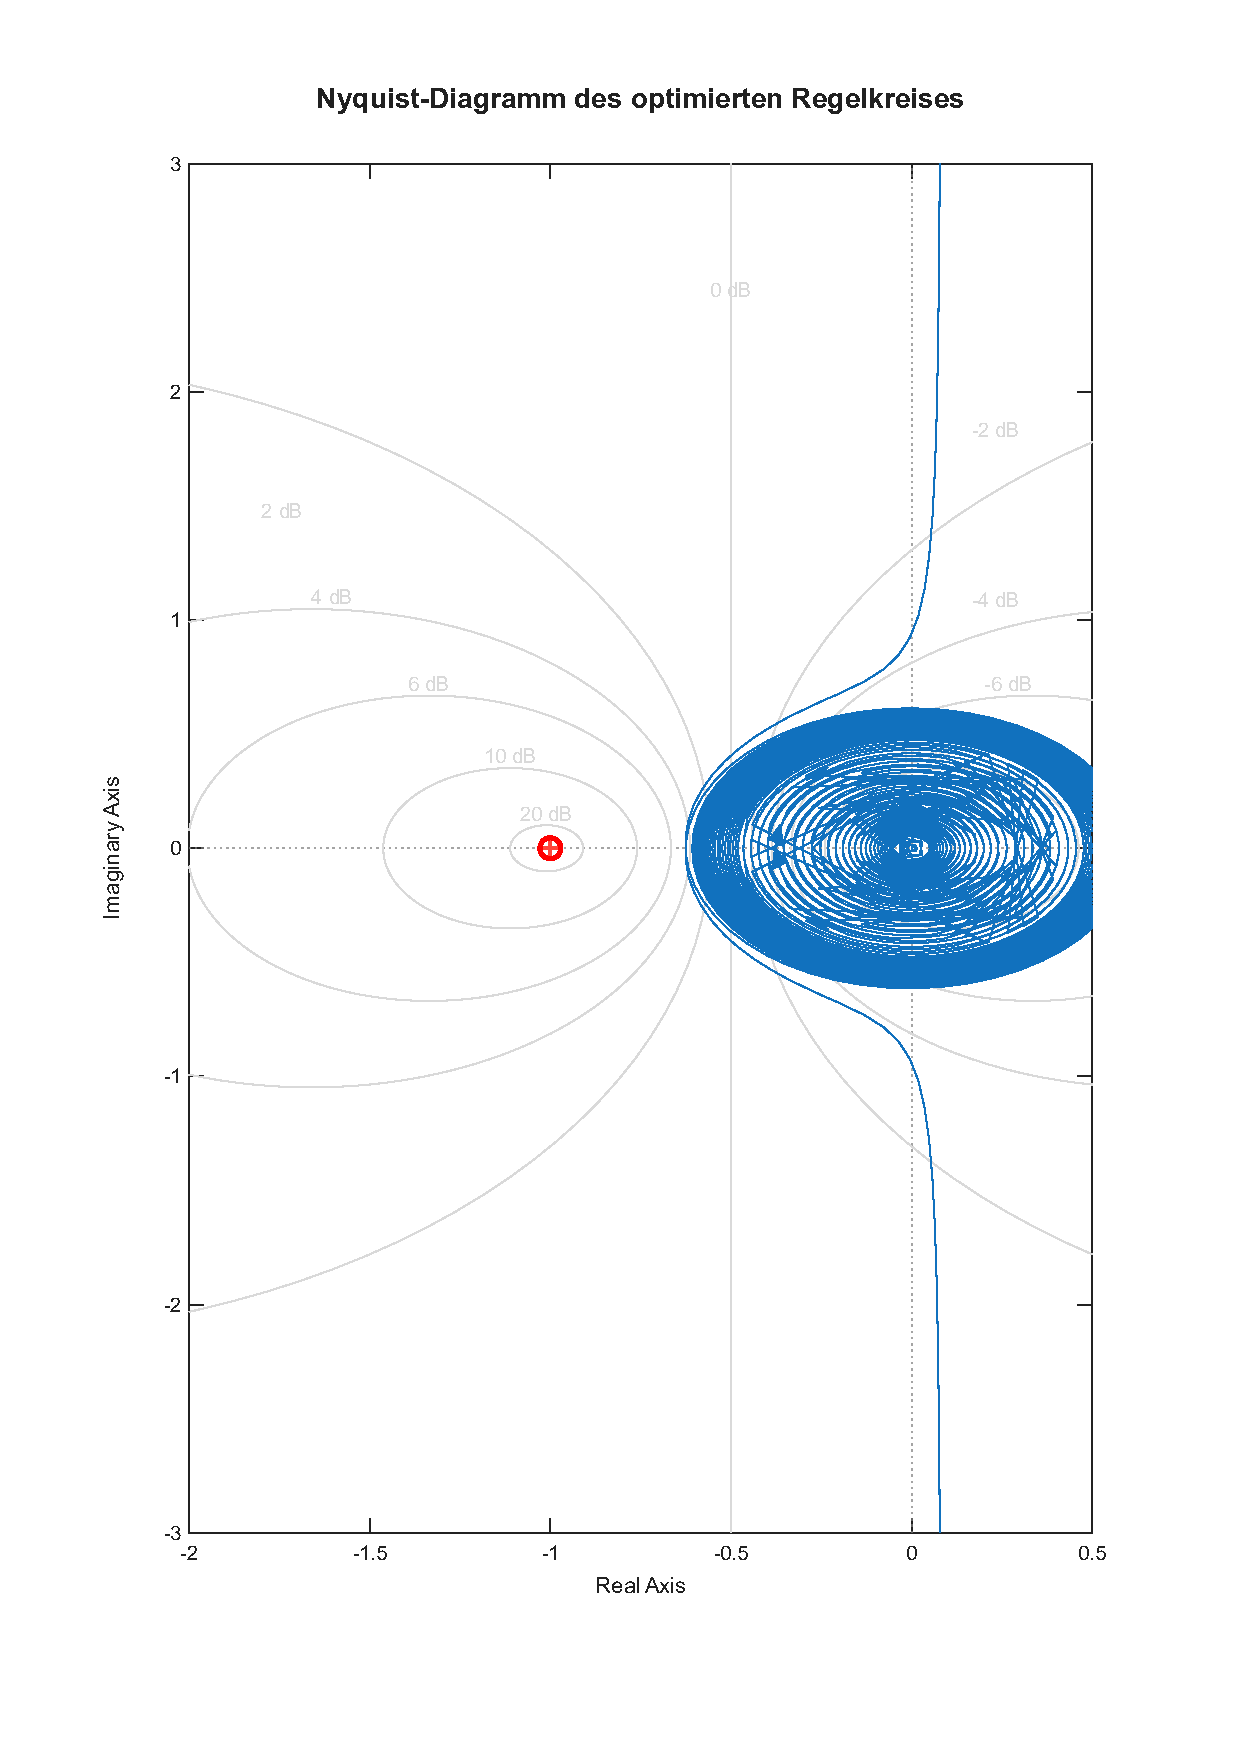
\includegraphics[width=0.8\textwidth]{Abbildungen/nyquist_aufgabe_7B_1.pdf}
    \caption{Nyquist-Diagramm mit Ziegler-Nichols-Regler}
    \label{fig:nyquist_7B1}
\end{figure}

Das Nyquist-Diagramm in Abbildung~\ref{fig:nyquist_7B1} zeigt, dass der geschlossene Regelkreis mit dem Ziegler-Nichols-Regler stabil ist, da die Kurve den kritischen Punkt $-1 + j0$ nicht umschließt. Allerdings ist die Phasenreserve deutlich geringer als beim Trial-and-Error-Versuch. 
Durch den geringeren I-Anteil, braucht die Todzeit länger um ausgeglichen zu werden, was zu einem dichterem Linienbündel führt.

\subsection{Aufgabe C -- Einfluss von Stellgrößenbeschränkungen}

Aufgabe C beschäftigt sich mit den Auswirkungen von Stellgrößenbeschränkungen auf das Regelverhalten.
Dies kann mit dem Saturation Block simuliert werden.
Es wurden zwei Sättigungsgrenzen untersucht:
\begin{itemize}
\item $c=\left[-3,3\right]$
\item $c2=\left[-1.5,1.5\right]$
\end{itemize}
\subsubsection{Versuchsaufbau und Durchführung}


Nach dem PID-Regler wird nun ein Saturation Block eingefügt, um die Ausgabe zu begrenzen.
\begin{figure}[H]
    \centering

    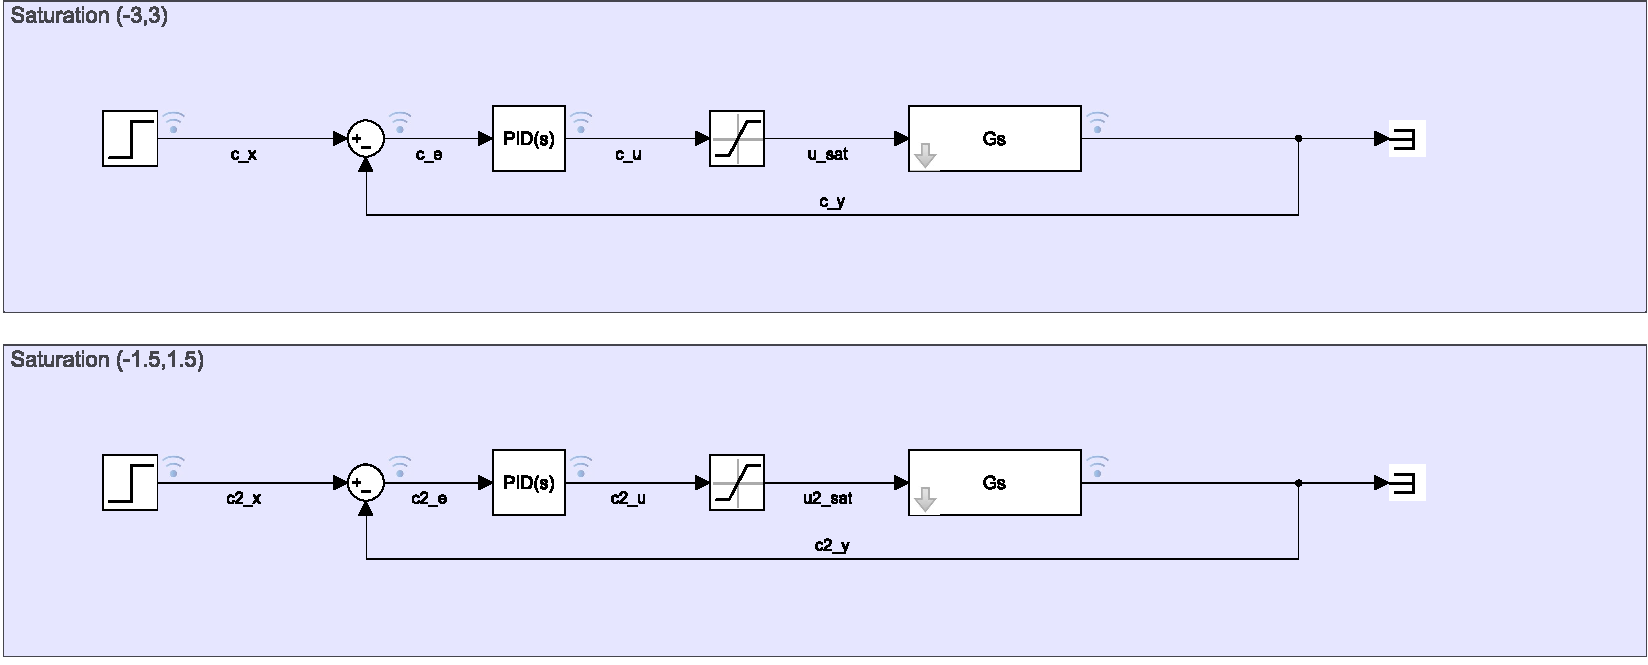
\includegraphics[width=1\textwidth]{Abbildungen/regelkreis_7_C1.pdf}
    \caption{Stellgrößenbeschränkung im Regelkreis}
    \label{fig:stelltbeschränkung_7C1}
\end{figure}

\begin{figure}[H]
    \centering

    % This file was created by matlab2tikz.
%
%The latest updates can be retrieved from
%  http://www.mathworks.com/matlabcentral/fileexchange/22022-matlab2tikz-matlab2tikz
%where you can also make suggestions and rate matlab2tikz.
%
\definecolor{mycolor1}{rgb}{0.92900,0.69400,0.12500}%
\definecolor{mycolor2}{rgb}{0.63500,0.07800,0.18400}%
\definecolor{mycolor3}{rgb}{0.12941,0.12941,0.12941}%
%
\begin{tikzpicture}

\begin{axis}[%
width=0.951\figurewidth,
height=\figureheight,
at={(0\figurewidth,0\figureheight)},
scale only axis,
xmin=0.00768049155146078,
xmax=6.0384024577573,
tick align=outside,
xlabel style={font=\color{mycolor3}},
xlabel={Time (seconds)},
ymin=-0.0119785962577792,
ymax=1.10714297230905,
axis background/.style={fill=white},
xmajorgrids,
ymajorgrids,
legend style={at={(0.145,0.935)}, anchor=south west, legend cell align=left, align=left}
]
\addplot[const plot, color=mycolor1, line width=2.0pt] table[row sep=crcr] {%
0	0\\
0.01	0\\
0.02	0\\
0.03	0\\
0.04	0\\
0.05	0\\
0.06	0\\
0.07	0\\
0.08	0\\
0.09	0\\
0.1	0\\
0.11	0\\
0.12	0\\
0.13	0\\
0.14	0\\
0.15	0\\
0.16	0\\
0.17	0\\
0.18	0\\
0.19	0\\
0.2	0\\
0.21	0\\
0.22	0\\
0.23	0\\
0.24	0\\
0.25	0\\
0.26	0\\
0.27	0\\
0.28	0\\
0.29	0\\
0.3	0\\
0.31	0\\
0.32	0\\
0.33	0\\
0.34	0\\
0.35	0\\
0.36	0\\
0.37	0\\
0.38	0\\
0.39	0\\
0.4	0\\
0.41	0\\
0.42	0\\
0.43	0\\
0.44	0\\
0.45	0\\
0.46	0\\
0.47	0\\
0.48	0\\
0.49	0\\
0.5	0\\
0.51	0\\
0.52	0\\
0.53	0\\
0.54	0\\
0.55	0\\
0.56	0\\
0.57	0\\
0.58	0\\
0.59	0\\
0.6	0\\
0.61	0\\
0.62	0\\
0.63	0\\
0.64	0\\
0.65	0\\
0.66	0\\
0.67	0\\
0.68	0\\
0.69	0\\
0.7	0\\
0.71	0\\
0.72	0\\
0.73	0\\
0.74	0\\
0.75	0\\
0.76	0\\
0.77	0\\
0.78	0\\
0.79	0\\
0.8	0\\
0.81	0\\
0.820000000000001	0\\
0.830000000000001	0\\
0.840000000000001	0\\
0.850000000000001	0\\
0.860000000000001	0\\
0.870000000000001	0\\
0.880000000000001	0\\
0.890000000000001	0\\
0.900000000000001	0\\
0.910000000000001	0\\
0.920000000000001	0\\
0.930000000000001	0\\
0.940000000000001	0\\
0.950000000000001	0\\
0.960000000000001	0\\
0.970000000000001	0\\
0.980000000000001	0\\
0.990000000000001	0\\
0.999999999999994	0\\
1	1\\
1.00706610368157	1\\
1.01413220736314	1\\
1.02274744349539	1\\
1.03274744349539	1\\
1.04274744349539	1\\
1.05274744349539	1\\
1.06274744349539	1\\
1.07274744349539	1\\
1.08274744349539	1\\
1.09274744349539	1\\
1.09602814589235	1\\
1.09602814589237	1\\
1.10602814589237	1\\
1.11602814589237	1\\
1.12602814589237	1\\
1.13602814589237	1\\
1.14602814589237	1\\
1.15602814589237	1\\
1.16602814589237	1\\
1.17602814589237	1\\
1.18602814589237	1\\
1.19602814589237	1\\
1.20602814589237	1\\
1.21602814589237	1\\
1.22602814589237	1\\
1.23602814589237	1\\
1.24602814589237	1\\
1.25602814589237	1\\
1.26602814589237	1\\
1.27602814589237	1\\
1.28602814589237	1\\
1.29602814589237	1\\
1.30602814589237	1\\
1.31602814589237	1\\
1.32516139939938	1\\
1.33516139939938	1\\
1.34516139939938	1\\
1.35516139939938	1\\
1.36516139939938	1\\
1.37516139939938	1\\
1.38516139939938	1\\
1.39516139939938	1\\
1.40516139939938	1\\
1.41516139939938	1\\
1.42516139939938	1\\
1.43516139939938	1\\
1.44516139939938	1\\
1.45516139939938	1\\
1.46516139939938	1\\
1.47516139939938	1\\
1.48516139939938	1\\
1.49516139939938	1\\
1.50516139939938	1\\
1.51516139939938	1\\
1.52516139939938	1\\
1.53516139939938	1\\
1.54516139939938	1\\
1.55516139939938	1\\
1.56516139939938	1\\
1.57516139939938	1\\
1.58516139939938	1\\
1.59516139939938	1\\
1.60516139939938	1\\
1.61516139939938	1\\
1.62516139939938	1\\
1.63516139939938	1\\
1.64516139939938	1\\
1.65516139939938	1\\
1.66516139939938	1\\
1.67516139939938	1\\
1.68516139939938	1\\
1.69516139939938	1\\
1.70516139939938	1\\
1.71516139939938	1\\
1.72516139939938	1\\
1.73516139939938	1\\
1.74516139939938	1\\
1.75516139939938	1\\
1.76516139939938	1\\
1.77516139939938	1\\
1.78516139939938	1\\
1.79516139939938	1\\
1.80516139939938	1\\
1.81516139939938	1\\
1.82516139939938	1\\
1.83516139939938	1\\
1.84516139939938	1\\
1.85516139939938	1\\
1.86516139939938	1\\
1.87516139939938	1\\
1.88516139939938	1\\
1.89516139939938	1\\
1.90516139939938	1\\
1.91516139939938	1\\
1.92516139939938	1\\
1.93516139939938	1\\
1.94516139939938	1\\
1.95516139939938	1\\
1.96516139939938	1\\
1.97516139939938	1\\
1.98516139939938	1\\
1.99516139939938	1\\
2.00516139939938	1\\
2.01516139939938	1\\
2.02516139939938	1\\
2.03516139939938	1\\
2.04516139939938	1\\
2.05516139939938	1\\
2.06516139939938	1\\
2.07516139939938	1\\
2.08516139939938	1\\
2.09516139939938	1\\
2.10516139939938	1\\
2.11516139939937	1\\
2.12516139939937	1\\
2.13516139939937	1\\
2.14516139939937	1\\
2.15516139939937	1\\
2.16516139939937	1\\
2.17516139939937	1\\
2.18516139939937	1\\
2.19516139939937	1\\
2.20516139939937	1\\
2.21516139939937	1\\
2.22516139939937	1\\
2.23516139939937	1\\
2.24516139939937	1\\
2.25516139939937	1\\
2.26516139939937	1\\
2.27516139939937	1\\
2.28516139939937	1\\
2.29516139939937	1\\
2.30516139939937	1\\
2.31516139939937	1\\
2.32516139939937	1\\
2.33516139939937	1\\
2.34516139939937	1\\
2.35516139939937	1\\
2.36516139939937	1\\
2.37516139939937	1\\
2.38516139939937	1\\
2.39516139939937	1\\
2.40516139939937	1\\
2.41516139939937	1\\
2.42516139939937	1\\
2.43516139939937	1\\
2.44516139939937	1\\
2.45516139939937	1\\
2.46516139939937	1\\
2.47516139939937	1\\
2.48516139939937	1\\
2.49516139939937	1\\
2.50516139939937	1\\
2.51516139939937	1\\
2.52516139939937	1\\
2.53516139939937	1\\
2.54516139939937	1\\
2.55516139939937	1\\
2.56516139939937	1\\
2.57516139939937	1\\
2.58516139939936	1\\
2.59516139939936	1\\
2.60516139939936	1\\
2.61516139939936	1\\
2.62516139939936	1\\
2.63516139939936	1\\
2.64516139939936	1\\
2.65516139939936	1\\
2.66516139939936	1\\
2.67516139939936	1\\
2.68516139939936	1\\
2.69516139939936	1\\
2.70516139939936	1\\
2.71516139939936	1\\
2.72516139939936	1\\
2.73516139939936	1\\
2.74516139939936	1\\
2.75516139939936	1\\
2.76516139939936	1\\
2.77516139939936	1\\
2.78516139939936	1\\
2.79516139939936	1\\
2.80516139939936	1\\
2.81516139939936	1\\
2.82516139939936	1\\
2.83516139939936	1\\
2.84516139939936	1\\
2.85516139939936	1\\
2.86516139939936	1\\
2.87516139939936	1\\
2.88516139939936	1\\
2.89516139939936	1\\
2.90516139939936	1\\
2.91516139939936	1\\
2.92516139939936	1\\
2.93516139939936	1\\
2.94516139939936	1\\
2.95516139939936	1\\
2.96516139939936	1\\
2.97516139939936	1\\
2.98516139939936	1\\
2.99516139939936	1\\
3.00516139939936	1\\
3.01516139939936	1\\
3.02516139939936	1\\
3.03516139939936	1\\
3.04516139939936	1\\
3.05516139939935	1\\
3.06516139939935	1\\
3.07516139939935	1\\
3.08516139939935	1\\
3.09516139939935	1\\
3.10516139939935	1\\
3.11516139939935	1\\
3.12516139939935	1\\
3.13516139939935	1\\
3.14516139939935	1\\
3.15516139939935	1\\
3.16516139939935	1\\
3.17516139939935	1\\
3.18516139939935	1\\
3.19516139939935	1\\
3.20516139939935	1\\
3.21516139939935	1\\
3.22516139939935	1\\
3.23516139939935	1\\
3.24516139939935	1\\
3.25516139939935	1\\
3.26516139939935	1\\
3.27516139939935	1\\
3.28516139939935	1\\
3.29516139939935	1\\
3.30516139939935	1\\
3.31516139939935	1\\
3.32516139939935	1\\
3.33516139939935	1\\
3.34516139939935	1\\
3.35516139939935	1\\
3.36516139939935	1\\
3.37516139939935	1\\
3.38516139939935	1\\
3.39516139939935	1\\
3.40516139939935	1\\
3.41516139939935	1\\
3.42516139939935	1\\
3.43516139939935	1\\
3.44516139939935	1\\
3.45516139939935	1\\
3.46516139939935	1\\
3.47516139939935	1\\
3.48516139939935	1\\
3.49516139939935	1\\
3.50516139939935	1\\
3.51516139939935	1\\
3.52516139939934	1\\
3.53516139939934	1\\
3.54516139939934	1\\
3.55516139939934	1\\
3.56516139939934	1\\
3.57516139939934	1\\
3.58516139939934	1\\
3.59516139939934	1\\
3.60516139939934	1\\
3.61516139939934	1\\
3.62516139939934	1\\
3.63516139939934	1\\
3.64516139939934	1\\
3.65516139939934	1\\
3.66516139939934	1\\
3.67516139939934	1\\
3.68516139939934	1\\
3.69516139939934	1\\
3.70516139939934	1\\
3.71516139939934	1\\
3.72516139939934	1\\
3.73516139939934	1\\
3.74516139939934	1\\
3.75516139939934	1\\
3.76516139939934	1\\
3.77516139939934	1\\
3.78516139939934	1\\
3.79516139939934	1\\
3.80516139939934	1\\
3.81516139939934	1\\
3.82516139939934	1\\
3.83516139939934	1\\
3.84516139939934	1\\
3.85516139939934	1\\
3.86516139939934	1\\
3.87516139939934	1\\
3.88516139939934	1\\
3.89516139939934	1\\
3.90516139939934	1\\
3.91516139939934	1\\
3.92516139939934	1\\
3.93516139939934	1\\
3.94516139939934	1\\
3.95516139939934	1\\
3.96516139939934	1\\
3.97516139939934	1\\
3.98516139939934	1\\
3.99516139939933	1\\
4.00516139939934	1\\
4.01516139939933	1\\
4.02516139939933	1\\
4.03516139939933	1\\
4.04516139939933	1\\
4.05516139939933	1\\
4.06516139939933	1\\
4.07516139939933	1\\
4.08516139939933	1\\
4.09516139939933	1\\
4.10516139939933	1\\
4.11516139939933	1\\
4.12516139939933	1\\
4.13516139939933	1\\
4.14516139939933	1\\
4.15516139939933	1\\
4.16516139939933	1\\
4.17516139939933	1\\
4.18516139939933	1\\
4.19516139939933	1\\
4.20516139939933	1\\
4.21516139939933	1\\
4.22516139939933	1\\
4.23516139939933	1\\
4.24516139939933	1\\
4.25516139939933	1\\
4.26516139939933	1\\
4.27516139939933	1\\
4.28516139939933	1\\
4.29516139939933	1\\
4.30516139939933	1\\
4.31516139939933	1\\
4.32516139939933	1\\
4.33516139939933	1\\
4.34516139939933	1\\
4.35516139939933	1\\
4.36516139939933	1\\
4.37516139939933	1\\
4.38516139939933	1\\
4.39516139939933	1\\
4.40516139939933	1\\
4.41516139939933	1\\
4.42516139939933	1\\
4.43516139939933	1\\
4.44516139939933	1\\
4.45516139939933	1\\
4.46516139939933	1\\
4.47516139939933	1\\
4.48516139939932	1\\
4.49516139939932	1\\
4.50516139939932	1\\
4.51516139939932	1\\
4.52516139939932	1\\
4.53516139939932	1\\
4.54516139939932	1\\
4.55516139939932	1\\
4.56516139939932	1\\
4.57516139939932	1\\
4.58516139939932	1\\
4.59516139939932	1\\
4.60516139939932	1\\
4.61516139939932	1\\
4.62516139939932	1\\
4.63516139939932	1\\
4.64516139939932	1\\
4.65516139939932	1\\
4.66516139939932	1\\
4.67516139939932	1\\
4.68516139939932	1\\
4.69516139939932	1\\
4.70516139939932	1\\
4.71516139939932	1\\
4.72516139939932	1\\
4.73516139939932	1\\
4.74516139939932	1\\
4.75516139939932	1\\
4.76516139939932	1\\
4.77516139939932	1\\
4.78516139939932	1\\
4.79516139939932	1\\
4.80516139939932	1\\
4.81516139939932	1\\
4.82516139939932	1\\
4.83516139939932	1\\
4.84516139939932	1\\
4.85516139939932	1\\
4.86516139939932	1\\
4.87516139939932	1\\
4.88516139939932	1\\
4.89516139939932	1\\
4.90516139939932	1\\
4.91516139939932	1\\
4.92516139939932	1\\
4.93516139939932	1\\
4.94516139939932	1\\
4.95516139939931	1\\
4.96516139939931	1\\
4.97516139939931	1\\
4.98516139939931	1\\
4.99516139939931	1\\
5.00516139939931	1\\
5.01516139939931	1\\
5.02516139939931	1\\
5.03516139939931	1\\
5.04516139939931	1\\
5.05516139939931	1\\
5.06516139939931	1\\
5.07516139939931	1\\
5.08516139939931	1\\
5.09516139939931	1\\
5.10516139939931	1\\
5.11516139939931	1\\
5.12516139939931	1\\
5.13516139939931	1\\
5.14516139939931	1\\
5.15516139939931	1\\
5.16516139939931	1\\
5.17516139939931	1\\
5.18516139939931	1\\
5.19516139939931	1\\
5.20516139939931	1\\
5.21516139939931	1\\
5.22516139939931	1\\
5.23516139939931	1\\
5.24516139939931	1\\
5.25516139939931	1\\
5.26516139939931	1\\
5.27516139939931	1\\
5.28516139939931	1\\
5.29516139939931	1\\
5.30516139939931	1\\
5.31516139939931	1\\
5.32516139939931	1\\
5.33516139939931	1\\
5.34516139939931	1\\
5.35516139939931	1\\
5.36516139939931	1\\
5.37516139939931	1\\
5.38516139939931	1\\
5.39516139939931	1\\
5.40516139939931	1\\
5.41516139939931	1\\
5.4251613993993	1\\
5.4351613993993	1\\
5.4451613993993	1\\
5.4551613993993	1\\
5.4651613993993	1\\
5.4751613993993	1\\
5.4851613993993	1\\
5.4951613993993	1\\
5.5051613993993	1\\
5.5151613993993	1\\
5.5251613993993	1\\
5.5351613993993	1\\
5.5451613993993	1\\
5.5551613993993	1\\
5.5651613993993	1\\
5.5751613993993	1\\
5.5851613993993	1\\
5.5951613993993	1\\
5.6051613993993	1\\
5.6151613993993	1\\
5.6251613993993	1\\
5.6351613993993	1\\
5.6451613993993	1\\
5.6551613993993	1\\
5.6651613993993	1\\
5.6751613993993	1\\
5.6851613993993	1\\
5.6951613993993	1\\
5.7051613993993	1\\
5.7151613993993	1\\
5.7251613993993	1\\
5.7351613993993	1\\
5.7451613993993	1\\
5.7551613993993	1\\
5.7651613993993	1\\
5.7751613993993	1\\
5.7851613993993	1\\
5.7951613993993	1\\
5.8051613993993	1\\
5.8151613993993	1\\
5.8251613993993	1\\
5.8351613993993	1\\
5.8451613993993	1\\
5.8551613993993	1\\
5.8651613993993	1\\
5.8751613993993	1\\
5.8851613993993	1\\
5.89516139939929	1\\
5.90516139939929	1\\
5.91516139939929	1\\
5.92516139939929	1\\
5.93516139939929	1\\
5.94516139939929	1\\
5.95516139939929	1\\
5.96516139939929	1\\
5.97516139939929	1\\
5.98516139939929	1\\
5.99516139939929	1\\
6.00516139939929	1\\
6.01516139939929	1\\
6.02516139939929	1\\
6.03516139939929	1\\
6.04516139939929	1\\
6.05516139939929	1\\
6.06516139939929	1\\
6.07516139939929	1\\
6.08516139939929	1\\
6.09516139939929	1\\
6.10516139939929	1\\
6.11516139939929	1\\
6.12516139939929	1\\
6.13516139939929	1\\
6.14516139939929	1\\
6.15516139939929	1\\
6.16516139939929	1\\
6.17516139939929	1\\
6.18516139939929	1\\
6.19516139939929	1\\
6.20516139939929	1\\
6.21516139939929	1\\
6.22516139939929	1\\
6.23516139939929	1\\
6.24516139939929	1\\
6.25516139939929	1\\
6.26516139939929	1\\
6.27516139939929	1\\
6.28516139939929	1\\
6.29516139939929	1\\
6.30516139939929	1\\
6.31516139939929	1\\
6.32516139939929	1\\
6.33516139939929	1\\
6.34516139939929	1\\
6.35516139939929	1\\
6.36516139939928	1\\
6.37516139939928	1\\
6.38516139939928	1\\
6.39516139939928	1\\
6.40516139939928	1\\
6.41516139939928	1\\
6.42516139939928	1\\
6.43516139939928	1\\
6.44516139939928	1\\
6.45516139939928	1\\
6.46516139939928	1\\
6.47516139939928	1\\
6.48516139939928	1\\
6.49516139939928	1\\
6.50516139939928	1\\
6.51516139939928	1\\
6.52516139939928	1\\
6.53516139939928	1\\
6.54516139939928	1\\
6.55516139939928	1\\
6.56516139939928	1\\
6.57516139939928	1\\
6.58516139939928	1\\
6.59516139939928	1\\
6.60516139939928	1\\
6.61516139939928	1\\
6.62516139939928	1\\
6.63516139939928	1\\
6.64516139939928	1\\
6.65516139939928	1\\
6.66516139939928	1\\
6.67516139939928	1\\
6.68516139939928	1\\
6.69516139939928	1\\
6.70516139939928	1\\
6.71516139939928	1\\
6.72516139939928	1\\
6.73516139939928	1\\
6.74516139939928	1\\
6.75516139939928	1\\
6.76516139939928	1\\
6.77516139939928	1\\
6.78516139939928	1\\
6.79516139939928	1\\
6.80516139939928	1\\
6.81516139939928	1\\
6.82516139939928	1\\
6.83516139939927	1\\
6.84516139939927	1\\
6.85516139939927	1\\
6.86516139939927	1\\
6.87516139939927	1\\
6.88516139939927	1\\
6.89516139939927	1\\
6.90516139939927	1\\
6.91516139939927	1\\
6.92516139939927	1\\
6.93516139939927	1\\
6.94516139939927	1\\
6.95516139939927	1\\
6.96516139939927	1\\
6.97516139939927	1\\
6.98516139939927	1\\
6.99516139939927	1\\
7.00516139939927	1\\
7.01516139939927	1\\
7.02516139939927	1\\
7.03516139939927	1\\
7.04516139939927	1\\
7.05516139939927	1\\
7.06516139939927	1\\
7.07516139939927	1\\
7.08516139939927	1\\
7.09516139939927	1\\
7.10516139939927	1\\
7.11516139939927	1\\
7.12516139939927	1\\
7.13516139939927	1\\
7.14516139939927	1\\
7.15516139939927	1\\
7.16516139939927	1\\
7.17516139939927	1\\
7.18516139939927	1\\
7.19516139939927	1\\
7.20516139939927	1\\
7.21516139939927	1\\
7.22516139939927	1\\
7.23516139939927	1\\
7.24516139939927	1\\
7.25516139939927	1\\
7.26516139939927	1\\
7.27516139939927	1\\
7.28516139939927	1\\
7.29516139939927	1\\
7.30516139939926	1\\
7.31516139939926	1\\
7.32516139939926	1\\
7.33516139939926	1\\
7.34516139939926	1\\
7.35516139939926	1\\
7.36516139939926	1\\
7.37516139939926	1\\
7.38516139939926	1\\
7.39516139939926	1\\
7.40516139939926	1\\
7.41516139939926	1\\
7.42516139939926	1\\
7.43516139939926	1\\
7.44516139939926	1\\
7.45516139939926	1\\
7.46516139939926	1\\
7.47516139939926	1\\
7.48516139939926	1\\
7.49516139939926	1\\
7.50516139939926	1\\
7.51516139939926	1\\
7.52516139939926	1\\
7.53516139939926	1\\
7.54516139939926	1\\
7.55516139939926	1\\
7.56516139939926	1\\
7.57516139939926	1\\
7.58516139939926	1\\
7.59516139939926	1\\
7.60516139939926	1\\
7.61516139939926	1\\
7.62516139939926	1\\
7.63516139939926	1\\
7.64516139939926	1\\
7.65516139939926	1\\
7.66516139939926	1\\
7.67516139939926	1\\
7.68516139939926	1\\
7.69516139939926	1\\
7.70516139939926	1\\
7.71516139939926	1\\
7.72516139939926	1\\
7.73516139939926	1\\
7.74516139939926	1\\
7.75516139939926	1\\
7.76516139939925	1\\
7.77516139939925	1\\
7.78516139939925	1\\
7.79516139939925	1\\
7.80516139939925	1\\
7.81516139939925	1\\
7.82516139939925	1\\
7.83516139939925	1\\
7.84516139939925	1\\
7.85516139939925	1\\
7.86516139939925	1\\
7.87516139939925	1\\
7.88516139939925	1\\
7.89516139939925	1\\
7.90516139939925	1\\
7.91516139939925	1\\
7.92516139939925	1\\
7.93516139939925	1\\
7.94516139939925	1\\
7.95516139939925	1\\
7.96516139939925	1\\
7.97516139939925	1\\
7.98516139939925	1\\
7.99516139939925	1\\
8.00516139939925	1\\
8.01516139939925	1\\
8.02516139939925	1\\
8.03516139939925	1\\
8.04516139939925	1\\
8.05516139939925	1\\
8.06516139939925	1\\
8.07516139939925	1\\
8.08516139939925	1\\
8.09516139939925	1\\
8.10516139939925	1\\
8.11516139939925	1\\
8.12516139939925	1\\
8.13516139939925	1\\
8.14516139939925	1\\
8.15516139939925	1\\
8.16516139939925	1\\
8.17516139939925	1\\
8.18516139939925	1\\
8.19516139939925	1\\
8.20516139939925	1\\
8.21516139939925	1\\
8.22516139939925	1\\
8.23516139939925	1\\
8.24516139939925	1\\
8.25516139939925	1\\
8.26516139939925	1\\
8.27516139939924	1\\
8.28516139939924	1\\
8.29516139939924	1\\
8.30516139939924	1\\
8.31516139939924	1\\
8.32516139939924	1\\
8.33516139939924	1\\
8.34516139939924	1\\
8.35516139939924	1\\
8.36516139939924	1\\
8.37516139939924	1\\
8.38516139939924	1\\
8.39516139939924	1\\
8.40516139939924	1\\
8.41516139939924	1\\
8.42516139939924	1\\
8.43516139939924	1\\
8.44516139939924	1\\
8.45516139939924	1\\
8.46516139939924	1\\
8.47516139939924	1\\
8.48516139939924	1\\
8.49516139939924	1\\
8.50516139939924	1\\
8.51516139939924	1\\
8.52516139939924	1\\
8.53516139939924	1\\
8.54516139939924	1\\
8.55516139939924	1\\
8.56516139939924	1\\
8.57516139939924	1\\
8.58516139939924	1\\
8.59516139939924	1\\
8.60516139939924	1\\
8.61516139939924	1\\
8.62516139939924	1\\
8.63516139939924	1\\
8.64516139939924	1\\
8.65516139939924	1\\
8.66516139939924	1\\
8.67516139939924	1\\
8.68516139939924	1\\
8.69516139939924	1\\
8.70516139939924	1\\
8.71516139939924	1\\
8.72516139939924	1\\
8.73516139939924	1\\
8.74516139939923	1\\
8.75516139939923	1\\
8.76516139939923	1\\
8.77516139939923	1\\
8.78516139939923	1\\
8.79516139939923	1\\
8.80516139939923	1\\
8.81516139939923	1\\
8.82516139939923	1\\
8.83516139939923	1\\
8.84516139939923	1\\
8.85516139939923	1\\
8.86516139939923	1\\
8.87516139939923	1\\
8.88516139939923	1\\
8.89516139939923	1\\
8.90516139939923	1\\
8.91516139939923	1\\
8.92516139939923	1\\
8.93516139939923	1\\
8.94516139939923	1\\
8.95516139939923	1\\
8.96516139939923	1\\
8.97516139939923	1\\
8.98516139939923	1\\
8.99516139939923	1\\
9.00516139939923	1\\
9.01516139939923	1\\
9.02516139939923	1\\
9.03516139939923	1\\
9.04516139939923	1\\
9.05516139939923	1\\
9.06516139939923	1\\
9.07516139939923	1\\
9.08516139939923	1\\
9.09516139939923	1\\
9.10516139939923	1\\
9.11516139939923	1\\
9.12516139939923	1\\
9.13516139939923	1\\
9.14516139939923	1\\
9.15516139939923	1\\
9.16516139939923	1\\
9.17516139939923	1\\
9.18516139939923	1\\
9.19516139939923	1\\
9.20516139939923	1\\
9.21516139939922	1\\
9.22516139939922	1\\
9.23516139939922	1\\
9.24516139939922	1\\
9.25516139939922	1\\
9.26516139939922	1\\
9.27516139939922	1\\
9.28516139939922	1\\
9.29516139939922	1\\
9.30516139939922	1\\
9.31516139939922	1\\
9.32516139939922	1\\
9.33516139939922	1\\
9.34516139939922	1\\
9.35516139939922	1\\
9.36516139939922	1\\
9.37516139939922	1\\
9.38516139939922	1\\
9.39516139939922	1\\
9.40516139939922	1\\
9.41516139939922	1\\
9.42516139939922	1\\
9.43516139939922	1\\
9.44516139939922	1\\
9.45516139939922	1\\
9.46516139939922	1\\
9.47516139939922	1\\
9.48516139939922	1\\
9.49516139939922	1\\
9.50516139939922	1\\
9.51516139939922	1\\
9.52516139939922	1\\
9.53516139939922	1\\
9.54516139939922	1\\
9.55516139939922	1\\
9.56516139939922	1\\
9.57516139939922	1\\
9.58516139939922	1\\
9.59516139939922	1\\
9.60516139939922	1\\
9.61516139939922	1\\
9.62516139939922	1\\
9.63516139939922	1\\
9.64516139939922	1\\
9.65516139939922	1\\
9.66516139939922	1\\
9.67516139939922	1\\
9.68516139939921	1\\
9.69516139939921	1\\
9.70516139939921	1\\
9.71516139939921	1\\
9.72516139939921	1\\
9.73516139939921	1\\
9.74516139939921	1\\
9.75516139939921	1\\
9.76516139939921	1\\
9.77516139939921	1\\
9.78516139939921	1\\
9.79516139939921	1\\
9.80516139939921	1\\
9.81516139939921	1\\
9.82516139939921	1\\
9.83516139939921	1\\
9.84516139939921	1\\
9.85516139939921	1\\
9.86516139939921	1\\
9.87516139939921	1\\
9.88516139939921	1\\
9.89516139939921	1\\
9.90516139939921	1\\
9.91516139939921	1\\
9.92516139939921	1\\
9.93516139939921	1\\
9.94516139939921	1\\
9.95516139939921	1\\
9.96516139939921	1\\
9.97516139939921	1\\
9.98516139939921	1\\
9.99516139939921	1\\
10	1\\
};
\addlegendentry{x}

\addplot [color=mycolor2, line width=2.0pt]
  table[row sep=crcr]{%
0	0\\
0.01	0\\
0.02	0\\
0.03	0\\
0.04	0\\
0.05	0\\
0.06	0\\
0.07	0\\
0.08	0\\
0.09	0\\
0.1	0\\
0.11	0\\
0.12	0\\
0.13	0\\
0.14	0\\
0.15	0\\
0.16	0\\
0.17	0\\
0.18	0\\
0.19	0\\
0.2	0\\
0.21	0\\
0.22	0\\
0.23	0\\
0.24	0\\
0.25	0\\
0.26	0\\
0.27	0\\
0.28	0\\
0.29	0\\
0.3	0\\
0.31	0\\
0.32	0\\
0.33	0\\
0.34	0\\
0.35	0\\
0.36	0\\
0.37	0\\
0.38	0\\
0.39	0\\
0.4	0\\
0.41	0\\
0.42	0\\
0.43	0\\
0.44	0\\
0.45	0\\
0.46	0\\
0.47	0\\
0.48	0\\
0.49	0\\
0.5	0\\
0.51	0\\
0.52	0\\
0.53	0\\
0.54	0\\
0.55	0\\
0.56	0\\
0.57	0\\
0.58	0\\
0.59	0\\
0.6	0\\
0.61	0\\
0.62	0\\
0.63	0\\
0.64	0\\
0.65	0\\
0.66	0\\
0.67	0\\
0.68	0\\
0.69	0\\
0.7	0\\
0.71	0\\
0.72	0\\
0.73	0\\
0.74	0\\
0.75	0\\
0.76	0\\
0.77	0\\
0.78	0\\
0.79	0\\
0.8	0\\
0.81	0\\
0.820000000000001	0\\
0.830000000000001	0\\
0.840000000000001	0\\
0.850000000000001	0\\
0.860000000000001	0\\
0.870000000000001	0\\
0.880000000000001	0\\
0.890000000000001	0\\
0.900000000000001	0\\
0.910000000000001	0\\
0.920000000000001	0\\
0.930000000000001	0\\
0.940000000000001	0\\
0.950000000000001	0\\
0.960000000000001	0\\
0.970000000000001	0\\
0.980000000000001	0\\
0.990000000000001	0\\
0.999999999999994	0\\
1	0\\
1.00706610368157	0\\
1.01413220736314	0\\
1.02274744349539	0\\
1.03274744349539	0\\
1.04274744349539	0\\
1.05274744349539	0\\
1.06274744349539	0\\
1.07274744349539	0\\
1.08274744349539	0\\
1.09274744349539	0\\
1.09602814589235	0\\
1.09602814589237	0\\
1.10602814589237	0\\
1.11602814589237	0\\
1.12602814589237	0\\
1.13602814589237	0\\
1.14602814589237	0\\
1.15602814589237	0\\
1.16602814589237	0\\
1.17602814589237	0\\
1.18602814589237	0\\
1.19602814589237	0\\
1.20602814589237	0\\
1.21602814589237	0\\
1.22602814589237	0\\
1.23602814589237	0\\
1.24602814589237	0\\
1.25602814589237	0\\
1.26602814589237	0\\
1.27602814589237	0\\
1.28602814589237	0\\
1.29602814589237	0\\
1.30602814589237	0.27919057230026\\
1.31602814589237	0.51632751428502\\
1.32516139939938	0.608452418163858\\
1.33516139939938	0.658066909330949\\
1.34516139939938	0.685993968490503\\
1.35516139939938	0.705967148041767\\
1.36516139939938	0.723043627235\\
1.37516139939938	0.739084840650097\\
1.38516139939938	0.754775174283626\\
1.39516139939938	0.770365045439093\\
1.40516139939938	0.785945364897296\\
1.41516139939938	0.801550560961474\\
1.42516139939938	0.817190641133265\\
1.43516139939938	0.832868492967683\\
1.44516139939938	0.848584202815111\\
1.45516139939938	0.864336863566729\\
1.46516139939938	0.880125239004936\\
1.47516139939938	0.895948007062218\\
1.48516139939938	0.911803848034537\\
1.49516139939938	0.927691475740707\\
1.50516139939938	0.943609647719108\\
1.51516139939938	0.959557167753369\\
1.52516139939938	0.975532885620774\\
1.53516139939938	0.991535695864063\\
1.54516139939938	1.00756453624802\\
1.55516139939938	1.02361838614278\\
1.56516139939938	1.03969626492116\\
1.57516139939938	1.05579723040076\\
1.58516139939938	1.0719203773404\\
1.59516139939938	1.08806483599309\\
1.60516139939938	1.06287542409583\\
1.61516139939938	0.936449416744884\\
1.62516139939938	0.829734329057749\\
1.63516139939938	0.767656963205372\\
1.64516139939938	0.734522065915431\\
1.65516139939938	0.716823227589198\\
1.66516139939938	0.706454127277495\\
1.67516139939938	0.699275706974797\\
1.68516139939938	0.69333882323766\\
1.69516139939938	0.687769345270754\\
1.70516139939938	0.682187483354247\\
1.71516139939938	0.67643312293936\\
1.72516139939938	0.670439444770165\\
1.73516139939938	0.664179159902034\\
1.74516139939938	0.657641364886966\\
1.75516139939938	0.650821861029494\\
1.76516139939938	0.643719159717642\\
1.77516139939938	0.63633285333904\\
1.78516139939938	0.628662957405964\\
1.79516139939938	0.620709647188316\\
1.80516139939938	0.612473153192946\\
1.81516139939938	0.603953720126457\\
1.82516139939938	0.595151591063372\\
1.83516139939938	0.586067001559771\\
1.84516139939938	0.576700177664483\\
1.85516139939938	0.567051335443302\\
1.86516139939938	0.557120681080493\\
1.87516139939938	0.546908411192161\\
1.88516139939938	0.53641471320959\\
1.89516139939938	0.525639765777955\\
1.90516139939938	0.523805630820558\\
1.91516139939938	0.556242086220522\\
1.92516139939938	0.617411763336175\\
1.93516139939938	0.674026850085384\\
1.94516139939938	0.715618463215588\\
1.95516139939938	0.743478738665233\\
1.96516139939938	0.762124889733594\\
1.97516139939938	0.775491964488406\\
1.98516139939938	0.7861552837887\\
1.99516139939938	0.795585777707418\\
2.00516139939938	0.80455846591353\\
2.01516139939938	0.813460698537561\\
2.02516139939938	0.822479617333727\\
2.03516139939938	0.831704249827322\\
2.04516139939938	0.841177238504803\\
2.05516139939938	0.850919913386624\\
2.06516139939938	0.860944032974958\\
2.07516139939938	0.871257138697447\\
2.08516139939938	0.881864945690282\\
2.09516139939938	0.892772391899744\\
2.10516139939938	0.903984091721876\\
2.11516139939937	0.915504529638624\\
2.12516139939937	0.927338141866936\\
2.13516139939937	0.939489350334279\\
2.14516139939937	0.951962576566174\\
2.15516139939937	0.964762247188145\\
2.16516139939937	0.977892795959344\\
2.17516139939937	0.991358664386759\\
2.18516139939937	1.00516430176731\\
2.19516139939937	1.0193141650057\\
2.20516139939937	1.03162049640178\\
2.21516139939937	1.03362777357985\\
2.22516139939937	1.0189720662874\\
2.23516139939937	0.993873531298353\\
2.24516139939937	0.968723287690452\\
2.25516139939937	0.948934529578652\\
2.26516139939937	0.935340485666157\\
2.27516139939937	0.926643630958685\\
2.28516139939937	0.921145120836957\\
2.29516139939937	0.917464023633993\\
2.30516139939937	0.914672833343942\\
2.31516139939937	0.912212330379096\\
2.32516139939937	0.909767743457757\\
2.33516139939937	0.907169390134949\\
2.34516139939937	0.904327626197114\\
2.35516139939937	0.901194707695145\\
2.36516139939937	0.897743958483371\\
2.37516139939937	0.893958949960919\\
2.38516139939937	0.889828091203497\\
2.39516139939937	0.885342004175684\\
2.40516139939937	0.880492280919521\\
2.41516139939937	0.875270906928026\\
2.42516139939937	0.869669998192962\\
2.43516139939937	0.86368168308792\\
2.44516139939937	0.857298050029246\\
2.45516139939937	0.850511124587474\\
2.46516139939937	0.843312859620937\\
2.47516139939937	0.835695131103442\\
2.48516139939937	0.827649736416001\\
2.49516139939937	0.819168393693918\\
2.50516139939937	0.810763875162532\\
2.51516139939937	0.805018559376641\\
2.52516139939937	0.805909524121238\\
2.53516139939937	0.814647187783099\\
2.54516139939937	0.828266848354597\\
2.55516139939937	0.84265257662257\\
2.56516139939937	0.855134478134116\\
2.57516139939937	0.864840017274585\\
2.58516139939936	0.872022752073448\\
2.59516139939936	0.87735859273652\\
2.60516139939936	0.881531059924427\\
2.61516139939936	0.885071817137202\\
2.62516139939936	0.888342145177171\\
2.63516139939936	0.891568152810817\\
2.64516139939936	0.894884465614668\\
2.65516139939936	0.898369513130141\\
2.66516139939936	0.902069464411497\\
2.67516139939936	0.906012903358275\\
2.68516139939936	0.910219233931928\\
2.69516139939936	0.914703259609371\\
2.70516139939936	0.91947758393491\\
2.71516139939936	0.9245538306451\\
2.72516139939936	0.929943248414622\\
2.73516139939936	0.935657004506714\\
2.74516139939936	0.941706325082346\\
2.75516139939936	0.948102561516941\\
2.76516139939936	0.954857221657018\\
2.77516139939936	0.961981984724721\\
2.78516139939936	0.969488708701155\\
2.79516139939936	0.977389434293309\\
2.80516139939936	0.985572503848212\\
2.81516139939936	0.993296632762127\\
2.82516139939936	0.998886095600141\\
2.83516139939936	1.00070722327804\\
2.84516139939936	0.998585511718153\\
2.85516139939936	0.993884241568365\\
2.86516139939936	0.988421103139939\\
2.87516139939936	0.983537377156456\\
2.88516139939936	0.979838820979512\\
2.89516139939936	0.977369138771479\\
2.90516139939936	0.975886189616601\\
2.91516139939936	0.97507093311052\\
2.92516139939936	0.974636899518055\\
2.93516139939936	0.974366843974986\\
2.94516139939936	0.974111243978682\\
2.95516139939936	0.973772910007865\\
2.96516139939936	0.973290252855385\\
2.97516139939936	0.972623931151028\\
2.98516139939936	0.971747645430851\\
2.99516139939936	0.970642338785825\\
3.00516139939936	0.969292767146116\\
3.01516139939936	0.967685564909346\\
3.02516139939936	0.965808193633547\\
3.03516139939936	0.963648387201556\\
3.04516139939936	0.961193865583764\\
3.05516139939935	0.958432189455089\\
3.06516139939935	0.955350686780495\\
3.07516139939935	0.951936415365715\\
3.08516139939935	0.948176143036778\\
3.09516139939935	0.944056336312087\\
3.10516139939935	0.939592602607415\\
3.11516139939935	0.934982714223955\\
3.12516139939935	0.930826106715553\\
3.13516139939935	0.928032546885322\\
3.14516139939935	0.927287872014495\\
3.15516139939935	0.92858751202643\\
3.16516139939935	0.931294383108536\\
3.17516139939935	0.934558385589185\\
3.18516139939935	0.937692751311743\\
3.19516139939935	0.940321752688567\\
3.20516139939935	0.942345760111165\\
3.21516139939935	0.94383520747464\\
3.22516139939935	0.944931292910531\\
3.23516139939935	0.945782074623016\\
3.24516139939935	0.946512508150834\\
3.25516139939935	0.947216682945019\\
3.26516139939935	0.947961022709225\\
3.27516139939935	0.948791102675518\\
3.28516139939935	0.949738373610985\\
3.29516139939935	0.950825434642392\\
3.30516139939935	0.952069692957649\\
3.31516139939935	0.953485709735405\\
3.32516139939935	0.955086620299104\\
3.33516139939935	0.956884957424959\\
3.34516139939935	0.9588931131302\\
3.35516139939935	0.96112359158076\\
3.36516139939935	0.963589145760971\\
3.37516139939935	0.966302851434095\\
3.38516139939935	0.969278148153736\\
3.39516139939935	0.972528863361305\\
3.40516139939935	0.976062227268975\\
3.41516139939935	0.97983471854986\\
3.42516139939935	0.983656275725271\\
3.43516139939935	0.987136155289661\\
3.44516139939935	0.989802293416471\\
3.45516139939935	0.991347667811586\\
3.46516139939935	0.991791902125379\\
3.47516139939935	0.991437417208363\\
3.48516139939935	0.990695675616079\\
3.49516139939935	0.98992356647813\\
3.50516139939935	0.989343789082311\\
3.51516139939935	0.989043961385203\\
3.52516139939934	0.989016021431968\\
3.53516139939934	0.989201869454477\\
3.54516139939934	0.989527924078575\\
3.55516139939934	0.989924924042389\\
3.56516139939934	0.990336049386063\\
3.57516139939934	0.990718016673358\\
3.58516139939934	0.991038939407576\\
3.59516139939934	0.991275294305217\\
3.60516139939934	0.991409134852233\\
3.61516139939934	0.991425943666882\\
3.62516139939934	0.991313137929109\\
3.63516139939934	0.991059098740282\\
3.64516139939934	0.990652571496802\\
3.65516139939934	0.990082308702545\\
3.66516139939934	0.989336862269304\\
3.67516139939934	0.988404463939074\\
3.68516139939934	0.987272955785578\\
3.69516139939934	0.985929748302164\\
3.70516139939934	0.98436345747279\\
3.71516139939934	0.982576235672623\\
3.72516139939934	0.980618957398033\\
3.73516139939934	0.978634479338737\\
3.74516139939934	0.976856182230252\\
3.75516139939934	0.975529685458197\\
3.76516139939934	0.974802811901253\\
3.77516139939934	0.974665333098021\\
3.78516139939934	0.974972717658715\\
3.79516139939934	0.975521795942361\\
3.80516139939934	0.976125439427696\\
3.81516139939934	0.976654868579452\\
3.82516139939934	0.97704729910609\\
3.83516139939934	0.977292224645649\\
3.84516139939934	0.977410989927187\\
3.85516139939934	0.977438927380752\\
3.86516139939934	0.977413495258821\\
3.87516139939934	0.977368173390355\\
3.88516139939934	0.977330413330435\\
3.89516139939934	0.977321855547733\\
3.90516139939934	0.977359500914361\\
3.91516139939934	0.977457066671376\\
3.92516139939934	0.977626168437047\\
3.93516139939934	0.977877218409539\\
3.94516139939934	0.978220052329855\\
3.95516139939934	0.978664342489183\\
3.96516139939934	0.979219859204788\\
3.97516139939934	0.979896632488502\\
3.98516139939934	0.980705051439863\\
3.99516139939933	0.981655926428264\\
4.00516139939934	0.982760134230656\\
4.01516139939933	0.984025270852179\\
4.02516139939933	0.985443861921374\\
4.03516139939933	0.986972383253269\\
4.04516139939933	0.988515761117459\\
4.05516139939933	0.989939647844537\\
4.06516139939933	0.991114075526606\\
4.07516139939933	0.991963196265912\\
4.08516139939933	0.99248954376965\\
4.09516139939933	0.992762291309903\\
4.10516139939933	0.99288307810376\\
4.11516139939933	0.992950723167248\\
4.12516139939933	0.993038781643429\\
4.13516139939933	0.993188634804454\\
4.14516139939933	0.99341359973704\\
4.15516139939933	0.993707804109478\\
4.16516139939933	0.994055129610716\\
4.17516139939933	0.994435920345395\\
4.18516139939933	0.994830998902702\\
4.19516139939933	0.995223493136216\\
4.20516139939933	0.995599248545032\\
4.21516139939933	0.995946505228234\\
4.22516139939933	0.996255301715483\\
4.23516139939933	0.996516863647884\\
4.24516139939933	0.996723090380517\\
4.25516139939933	0.996866167983291\\
4.26516139939933	0.996938296718084\\
4.27516139939933	0.996931507287221\\
4.28516139939933	0.996837539749034\\
4.29516139939933	0.996647763834082\\
4.30516139939933	0.996353219279541\\
4.31516139939933	0.995945484869712\\
4.32516139939933	0.995420392324045\\
4.33516139939933	0.994786498020087\\
4.34516139939933	0.994075743132267\\
4.35516139939933	0.993347549367169\\
4.36516139939933	0.992678274469678\\
4.37516139939933	0.992138162397763\\
4.38516139939933	0.991768250697762\\
4.39516139939933	0.991569850772534\\
4.40516139939933	0.991510125383449\\
4.41516139939933	0.991537936976183\\
4.42516139939933	0.991600947866493\\
4.43516139939933	0.991657554187984\\
4.44516139939933	0.991681764978835\\
4.45516139939933	0.991662468076102\\
4.46516139939933	0.991599731242846\\
4.47516139939933	0.991500446530624\\
4.48516139939932	0.991374683150899\\
4.49516139939932	0.991233234082475\\
4.50516139939932	0.991086287481282\\
4.51516139939932	0.990942919850716\\
4.52516139939932	0.990811082838333\\
4.53516139939932	0.990697826731521\\
4.54516139939932	0.990609596140219\\
4.55516139939932	0.990552510673322\\
4.56516139939932	0.990532595377655\\
4.57516139939932	0.990555954992659\\
4.58516139939932	0.990628899501817\\
4.59516139939932	0.990758032569754\\
4.60516139939932	0.99095029161322\\
4.61516139939932	0.991212752594732\\
4.62516139939932	0.991551524916562\\
4.63516139939932	0.991968668616291\\
4.64516139939932	0.992456985702646\\
4.65516139939932	0.992995120544963\\
4.66516139939932	0.99354731290001\\
4.67516139939932	0.994070386925919\\
4.68516139939932	0.994525727626426\\
4.69516139939932	0.994890333334682\\
4.70516139939932	0.995161698871251\\
4.71516139939932	0.995355239402401\\
4.72516139939932	0.995496800577459\\
4.73516139939932	0.995614214913267\\
4.74516139939932	0.995730934591095\\
4.75516139939932	0.995862896954179\\
4.76516139939932	0.996018231153976\\
4.77516139939932	0.996198698213915\\
4.78516139939932	0.996401752152375\\
4.79516139939932	0.996622462058077\\
4.80516139939932	0.996854939096328\\
4.81516139939932	0.997093210254352\\
4.82516139939932	0.997331638319199\\
4.83516139939932	0.997565036030855\\
4.84516139939932	0.997788608745111\\
4.85516139939932	0.997997822643766\\
4.86516139939932	0.998188257330438\\
4.87516139939932	0.998355472260494\\
4.88516139939932	0.998494897595014\\
4.89516139939932	0.998601749830065\\
4.90516139939932	0.998670973415169\\
4.91516139939932	0.998697255581438\\
4.92516139939932	0.998675325664278\\
4.93516139939932	0.998600992161196\\
4.94516139939932	0.998473317286803\\
4.95516139939931	0.998297542637044\\
4.96516139939931	0.998087180873633\\
4.97516139939931	0.997863304401213\\
4.98516139939931	0.997650338957824\\
4.99516139939931	0.99746984085966\\
5.00516139939931	0.99733504705862\\
5.01516139939931	0.997248468211029\\
5.02516139939931	0.997203042680532\\
5.03516139939931	0.997185721911077\\
5.04516139939931	0.997181697533348\\
5.05516139939931	0.997177809608949\\
5.06516139939931	0.997164467017676\\
5.07516139939931	0.997136135434677\\
5.08516139939931	0.997090846580411\\
5.09516139939931	0.997029256692358\\
5.10516139939931	0.996953661747055\\
5.11516139939931	0.996867197591435\\
5.12516139939931	0.996773300327973\\
5.13516139939931	0.996675407181385\\
5.14516139939931	0.996576836774845\\
5.15516139939931	0.996480782405895\\
5.16516139939931	0.996390364349204\\
5.17516139939931	0.996308704614563\\
5.18516139939931	0.996239003118585\\
5.19516139939931	0.996184605436723\\
5.20516139939931	0.996149057934376\\
5.21516139939931	0.99613613705661\\
5.22516139939931	0.996149789082209\\
5.23516139939931	0.996193811065607\\
5.24516139939931	0.996271032689417\\
5.25516139939931	0.996381924588617\\
5.26516139939931	0.996523039945071\\
5.27516139939931	0.996686180365461\\
5.28516139939931	0.996859134923134\\
5.29516139939931	0.997028102706857\\
5.30516139939931	0.99718094843741\\
5.31516139939931	0.997309964366317\\
5.32516139939931	0.997413117912388\\
5.33516139939931	0.997493557091935\\
5.34516139939931	0.997557880980181\\
5.35516139939931	0.997614002453351\\
5.36516139939931	0.997669319006453\\
5.37516139939931	0.997729568128537\\
5.38516139939931	0.997798402373087\\
5.39516139939931	0.997877504966777\\
5.40516139939931	0.997966999068143\\
5.41516139939931	0.998065937759416\\
5.4251613993993	0.998172738533925\\
5.4351613993993	0.998285501740735\\
5.4451613993993	0.998402206242689\\
5.4551613993993	0.998520804110922\\
5.4651613993993	0.998639245263882\\
5.4751613993993	0.998755460597767\\
5.4851613993993	0.998867325028438\\
5.4951613993993	0.998972614176569\\
5.5051613993993	0.999068962475359\\
5.5151613993993	0.999153829529743\\
5.5251613993993	0.999224494840558\\
5.5351613993993	0.999278140054341\\
5.5451613993993	0.999312128446791\\
5.5551613993993	0.999324584726867\\
5.5651613993993	0.999315234387588\\
5.5751613993993	0.999286209342601\\
5.5851613993993	0.999242354078641\\
5.5951613993993	0.999190677499599\\
5.6051613993993	0.999138987372846\\
5.6151613993993	0.999094170642756\\
5.6251613993993	0.9990607594595\\
5.6351613993993	0.999040257909649\\
5.6451613993993	0.99903133854649\\
5.6551613993993	0.999030679179306\\
5.6651613993993	0.999034050747101\\
5.6751613993993	0.99903730080008\\
5.6851613993993	0.999037023842548\\
5.6951613993993	0.999030871534958\\
5.7051613993993	0.999017568969831\\
5.7151613993993	0.998996750530285\\
5.7251613993993	0.998968724367152\\
5.7351613993993	0.99893424335372\\
5.7451613993993	0.998894324018553\\
5.7551613993993	0.998850125841338\\
5.7651613993993	0.998802885429456\\
5.7751613993993	0.998753892262255\\
5.7851613993993	0.99870449162545\\
5.7951613993993	0.998656102783584\\
5.8051613993993	0.998610243903162\\
5.8151613993993	0.998568557663251\\
5.8251613993993	0.998532829318984\\
5.8351613993993	0.998504976486073\\
5.8451613993993	0.99848696619534\\
5.8551613993993	0.998480598095007\\
5.8651613993993	0.99848712085343\\
5.8751613993993	0.998506743665482\\
5.8851613993993	0.998538225751275\\
5.89516139939929	0.998578778239056\\
5.90516139939929	0.998624423511172\\
5.91516139939929	0.998670756970093\\
5.92516139939929	0.998713864756863\\
5.93516139939929	0.99875108399456\\
5.94516139939929	0.99878137748767\\
5.95516139939929	0.998805266905555\\
5.96516139939929	0.998824428639148\\
5.97516139939929	0.998841137903823\\
5.98516139939929	0.998857739501172\\
5.99516139939929	0.99887626000851\\
6.00516139939929	0.998898199204506\\
6.01516139939929	0.998924479386783\\
6.02516139939929	0.998955501527464\\
6.03516139939929	0.998991253395985\\
6.04516139939929	0.999031426492725\\
6.05516139939929	0.999075515560792\\
6.06516139939929	0.999122889676082\\
6.07516139939929	0.999172834427642\\
6.08516139939929	0.999224570260353\\
6.09516139939929	0.999277253836935\\
6.10516139939929	0.999329968817135\\
6.11516139939929	0.999381711207178\\
6.12516139939929	0.999431374142186\\
6.13516139939929	0.999477740270102\\
6.14516139939929	0.999519499051225\\
6.15516139939929	0.999555318013554\\
6.16516139939929	0.999583998001222\\
6.17516139939929	0.99960471587732\\
6.18516139939929	0.99961730313608\\
6.19516139939929	0.999622454388221\\
6.20516139939929	0.999621749985281\\
6.21516139939929	0.999617434598527\\
6.22516139939929	0.999611994266955\\
6.23516139939929	0.999607661807033\\
6.24516139939929	0.999606006560328\\
6.25516139939929	0.999607721050998\\
6.26516139939929	0.999612634815617\\
6.27516139939929	0.999619908225915\\
6.28516139939929	0.999628316926243\\
6.29516139939929	0.999636536595058\\
6.30516139939929	0.99964336525197\\
6.31516139939929	0.999647857038986\\
6.32516139939929	0.999649372082407\\
6.33516139939929	0.999647564701175\\
6.34516139939929	0.999642337105243\\
6.35516139939929	0.999633781950683\\
6.36516139939928	0.999622129523975\\
6.37516139939928	0.999607707588629\\
6.38516139939928	0.999590916001705\\
6.39516139939928	0.999572214623368\\
6.40516139939928	0.999552121468348\\
6.41516139939928	0.999531217780698\\
6.42516139939928	0.999510156843349\\
6.43516139939928	0.999489672598366\\
6.44516139939928	0.999470581077714\\
6.45516139939928	0.999453762027815\\
6.46516139939928	0.999440103565143\\
6.47516139939928	0.999430396887788\\
6.48516139939928	0.999425187097547\\
6.49516139939928	0.999424615843428\\
6.50516139939928	0.999428314855457\\
6.51516139939928	0.999435407090656\\
6.52516139939928	0.999444638342568\\
6.53516139939928	0.999454611671325\\
6.54516139939928	0.999464056358129\\
6.55516139939928	0.999472052581331\\
6.56516139939928	0.999478154893235\\
6.57516139939928	0.999482397522888\\
6.58516139939928	0.999485202675398\\
6.59516139939928	0.999487235172785\\
6.60516139939928	0.999489249419749\\
6.61516139939928	0.999491962918949\\
6.62516139939928	0.99949597304552\\
6.63516139939928	0.999501717967404\\
6.64516139939928	0.999509472446238\\
6.65516139939928	0.999519365339298\\
6.66516139939928	0.999531406397037\\
6.67516139939928	0.99954551319626\\
6.68516139939928	0.999561532871282\\
6.69516139939928	0.999579256536273\\
6.70516139939928	0.99959842646952\\
6.71516139939928	0.999618737287994\\
6.72516139939928	0.999639832812063\\
6.73516139939928	0.999661300677095\\
6.74516139939928	0.999682667771797\\
6.75516139939928	0.99970340187668\\
6.76516139939928	0.999722927862073\\
6.77516139939928	0.999740667834669\\
6.78516139939928	0.999756109901569\\
6.79516139939928	0.999768898191939\\
6.80516139939928	0.999778921491276\\
6.81516139939928	0.999786368298982\\
6.82516139939928	0.999791720505539\\
6.83516139939927	0.999795676950072\\
6.84516139939927	0.999799023513756\\
6.85516139939927	0.999802485706569\\
6.86516139939927	0.999806604121842\\
6.87516139939927	0.999811662147339\\
6.88516139939927	0.999817675688902\\
6.89516139939927	0.999824435579455\\
6.90516139939927	0.999831581569524\\
6.91516139939927	0.999838684374648\\
6.92516139939927	0.999845317168329\\
6.93516139939927	0.999851106250658\\
6.94516139939927	0.999855758745984\\
6.95516139939927	0.999859070890978\\
6.96516139939927	0.999860923172202\\
6.97516139939927	0.999861268782431\\
6.98516139939927	0.999860120577727\\
6.99516139939927	0.999857539886397\\
7.00516139939927	0.99985362880865\\
7.01516139939927	0.999848526375162\\
7.02516139939927	0.99984240814747\\
7.03516139939927	0.999835488374245\\
7.04516139939927	0.999828023322324\\
7.05516139939927	0.99982031347334\\
7.06516139939927	0.999812700789966\\
7.07516139939927	0.999805555883725\\
7.08516139939927	0.999799250270594\\
7.09516139939927	0.999794112634966\\
7.10516139939927	0.999790375113723\\
7.11516139939927	0.999788123266115\\
7.12516139939927	0.999787267076198\\
7.13516139939927	0.999787546691285\\
7.14516139939927	0.999788576116598\\
7.15516139939927	0.999789915230721\\
7.16516139939927	0.999791151130202\\
7.17516139939927	0.999791967853053\\
7.18516139939927	0.99979218903347\\
7.19516139939927	0.999791787793401\\
7.20516139939927	0.999790867848504\\
7.21516139939927	0.999789626114002\\
7.22516139939927	0.999788308879811\\
7.23516139939927	0.999787171653565\\
7.24516139939927	0.99978644881591\\
7.25516139939927	0.99978633508108\\
7.26516139939927	0.999786977597165\\
7.27516139939927	0.999788475796761\\
7.28516139939927	0.99979088568342\\
7.29516139939927	0.999794225684115\\
7.30516139939926	0.999798482043273\\
7.31516139939926	0.999803612618165\\
7.32516139939926	0.999809548656745\\
7.33516139939926	0.999816194651418\\
7.34516139939926	0.999823426755429\\
7.35516139939926	0.999831090709925\\
7.36516139939926	0.999839000930453\\
7.37516139939926	0.999846943270933\\
7.38516139939926	0.999854684498264\\
7.39516139939926	0.99986199079971\\
7.40516139939926	0.999868655083594\\
7.41516139939926	0.999874528827351\\
7.42516139939926	0.99987955046535\\
7.43516139939926	0.999883761007737\\
7.44516139939926	0.999887300072405\\
7.45516139939926	0.9998903812079\\
7.46516139939926	0.999893251948857\\
7.47516139939926	0.999896148674728\\
7.48516139939926	0.999899257266902\\
7.49516139939926	0.999902687808401\\
7.50516139939926	0.999906466681211\\
7.51516139939926	0.999910544460838\\
7.52516139939926	0.999914814605725\\
7.53516139939926	0.999919136741673\\
7.54516139939926	0.999923359073901\\
7.55516139939926	0.999927336318976\\
7.56516139939926	0.999930941659858\\
7.57516139939926	0.999934072953814\\
7.58516139939926	0.999936654475579\\
7.59516139939926	0.999938635862558\\
7.60516139939926	0.99993998982232\\
7.61516139939926	0.999940709790976\\
7.62516139939926	0.999940808285611\\
7.63516139939926	0.999940316291426\\
7.64516139939926	0.999939283695987\\
7.65516139939926	0.999937780482008\\
7.66516139939926	0.999935898026481\\
7.67516139939926	0.999933749380417\\
7.68516139939926	0.999931466937069\\
7.69516139939926	0.999929195778414\\
7.70516139939926	0.999927081651762\\
7.71516139939926	0.999925254155184\\
7.72516139939926	0.999923807914604\\
7.73516139939926	0.999922786362249\\
7.74516139939926	0.999922173113676\\
7.75516139939926	0.9999218943781\\
7.76516139939925	0.999921832759249\\
7.77516139939925	0.999921849420441\\
7.78516139939925	0.99992180925144\\
7.79516139939925	0.999921603208631\\
7.80516139939925	0.999921163372065\\
7.81516139939925	0.999920468731847\\
7.82516139939925	0.999919542278218\\
7.83516139939925	0.999918441814405\\
7.84516139939925	0.999917247675781\\
7.85516139939925	0.99991605030782\\
7.86516139939925	0.999914939791721\\
7.87516139939925	0.99991399833928\\
7.88516139939925	0.999913295844362\\
7.89516139939925	0.999912887954742\\
7.90516139939925	0.999912815843619\\
7.91516139939925	0.999913106846788\\
7.92516139939925	0.999913775283276\\
7.93516139939925	0.99991482299637\\
7.94516139939925	0.999916239374695\\
7.95516139939925	0.99991800082145\\
7.96516139939925	0.999920069856119\\
7.97516139939925	0.99992239429228\\
7.98516139939925	0.999924907231472\\
7.99516139939925	0.99992752884358\\
8.00516139939925	0.999930170867903\\
8.01516139939925	0.99993274426831\\
8.02516139939925	0.999935169489951\\
8.03516139939925	0.999937387572305\\
8.04516139939925	0.999939369492279\\
8.05516139939925	0.999941121045363\\
8.06516139939925	0.999942681508575\\
8.07516139939925	0.999944115989082\\
8.08516139939925	0.999945503123879\\
8.09516139939925	0.99994692099726\\
8.10516139939925	0.999948434392709\\
8.11516139939925	0.999950085814015\\
8.12516139939925	0.999951891456413\\
8.13516139939925	0.999953841974293\\
8.14516139939925	0.999955906887453\\
8.15516139939925	0.999958040994673\\
8.16516139939925	0.999960191205022\\
8.17516139939925	0.999962302590912\\
8.18516139939925	0.99996432300277\\
8.19516139939925	0.999966206086132\\
8.20516139939925	0.999967912903481\\
8.21516139939925	0.999969412554787\\
8.22516139939925	0.999970682235291\\
8.23516139939925	0.999971707114547\\
8.24516139939925	0.999972480315363\\
8.25516139939925	0.999973003148018\\
8.26516139939925	0.99997328562375\\
8.27516139939924	0.999973347123552\\
8.28516139939924	0.999973216925766\\
8.29516139939924	0.99997293412098\\
8.30516139939924	0.999972546339015\\
8.31516139939924	0.999972106790739\\
8.32516139939924	0.999971669470093\\
8.33516139939924	0.999971282941589\\
8.34516139939924	0.999970983777718\\
8.35516139939924	0.999970791134243\\
8.36516139939924	0.999970703921663\\
8.37516139939924	0.999970701485918\\
8.38516139939924	0.999970747815188\\
8.39516139939924	0.999970798363506\\
8.40516139939924	0.999970807953205\\
8.41516139939924	0.999970738077173\\
8.42516139939924	0.999970562258875\\
8.43516139939924	0.999970268767796\\
8.44516139939924	0.999969860686933\\
8.45516139939924	0.999969353877873\\
8.46516139939924	0.999968773675875\\
8.47516139939924	0.999968151167621\\
8.48516139939924	0.999967519729892\\
8.49516139939924	0.999966912240797\\
8.50516139939924	0.999966359108776\\
8.51516139939924	0.999965887058547\\
8.52516139939924	0.999965518490936\\
8.53516139939924	0.999965271189831\\
8.54516139939924	0.999965158163973\\
8.55516139939924	0.999965187460864\\
8.56516139939924	0.999965361858763\\
8.57516139939924	0.999965678424907\\
8.58516139939924	0.999966128025326\\
8.59516139939924	0.999966694980756\\
8.60516139939924	0.999967357161736\\
8.61516139939924	0.999968086856692\\
8.62516139939924	0.999968852672038\\
8.63516139939924	0.999969622502179\\
8.64516139939924	0.99997036727285\\
8.65516139939924	0.99997106482028\\
8.66516139939924	0.99997170306511\\
8.67516139939924	0.999972281685577\\
8.68516139939924	0.999972811806786\\
8.69516139939924	0.999973313707721\\
8.70516139939924	0.999973813039212\\
8.71516139939924	0.99997433638047\\
8.72516139939924	0.999974907044409\\
8.73516139939924	0.999975541876843\\
8.74516139939923	0.999976249467328\\
8.75516139939923	0.999977029821625\\
8.76516139939923	0.99997787524506\\
8.77516139939923	0.999978772014685\\
8.78516139939923	0.999979702384962\\
8.79516139939923	0.999980646545586\\
8.80516139939923	0.999981584281305\\
8.81516139939923	0.999982496224064\\
8.82516139939923	0.999983364703612\\
8.83516139939923	0.999984174277962\\
8.84516139939923	0.999984912058774\\
8.85516139939923	0.999985567946995\\
8.86516139939923	0.999986134871056\\
8.87516139939923	0.999986609081362\\
8.88516139939923	0.999986990503835\\
8.89516139939923	0.999987283093459\\
8.90516139939923	0.999987495062495\\
8.91516139939923	0.999987638804604\\
8.92516139939923	0.999987730324218\\
8.93516139939923	0.999987788038688\\
8.94516139939923	0.999987830958291\\
8.95516139939923	0.999987876439646\\
8.96516139939923	0.999987937889755\\
8.97516139939923	0.999988022896022\\
8.98516139939923	0.999988132219558\\
8.99516139939923	0.999988259912156\\
9.00516139939923	0.999988394554287\\
9.01516139939923	0.999988521348161\\
9.02516139939923	0.9999886246195\\
9.03516139939923	0.999988690231985\\
9.04516139939923	0.999988707498342\\
9.05516139939923	0.999988670339703\\
9.06516139939923	0.999988577639098\\
9.07516139939923	0.99998843289989\\
9.08516139939923	0.999988243421254\\
9.09516139939923	0.99998801923242\\
9.10516139939923	0.999987771998351\\
9.11516139939923	0.99998751404592\\
9.12516139939923	0.999987257586157\\
9.13516139939923	0.999987014143857\\
9.14516139939923	0.999986794160729\\
9.15516139939923	0.999986606714893\\
9.16516139939923	0.999986459295297\\
9.17516139939923	0.999986357580134\\
9.18516139939923	0.999986305190352\\
9.19516139939923	0.999986303420595\\
9.20516139939923	0.999986350988108\\
9.21516139939922	0.999986443879198\\
9.22516139939922	0.999986575400687\\
9.23516139939922	0.999986736544078\\
9.24516139939922	0.999986916729064\\
9.25516139939922	0.999987104909573\\
9.26516139939922	0.999987290917921\\
9.27516139939922	0.999987466825661\\
9.28516139939922	0.999987628052093\\
9.29516139939922	0.999987773978102\\
9.30516139939922	0.999987907922424\\
9.31516139939922	0.999988036480656\\
9.32516139939922	0.999988168369538\\
9.33516139939922	0.999988313017608\\
9.34516139939922	0.999988479173697\\
9.35516139939922	0.999988673766604\\
9.36516139939922	0.999988901163443\\
9.37516139939922	0.999989162871355\\
9.38516139939922	0.999989457636697\\
9.39516139939922	0.9999897818365\\
9.40516139939922	0.999990130034759\\
9.41516139939922	0.999990495585917\\
9.42516139939922	0.999990871198214\\
9.43516139939922	0.999991249407545\\
9.44516139939922	0.99999162294788\\
9.45516139939922	0.999991985030708\\
9.46516139939922	0.999992329561186\\
9.47516139939922	0.999992651323047\\
9.48516139939922	0.99999294615944\\
9.49516139939922	0.999993211164241\\
9.50516139939922	0.999993444879369\\
9.51516139939922	0.999993647470616\\
9.52516139939922	0.999993820832056\\
9.53516139939922	0.999993968555132\\
9.54516139939922	0.999994095701998\\
9.55516139939922	0.999994208350091\\
9.56516139939922	0.99999431292466\\
9.57516139939922	0.999994415396554\\
9.58516139939922	0.999994520474542\\
9.59516139939922	0.999994630944752\\
9.60516139939922	0.999994747292657\\
9.61516139939922	0.999994867687364\\
9.62516139939922	0.999994988329765\\
9.63516139939922	0.999995104088689\\
9.64516139939922	0.999995209294708\\
9.65516139939922	0.999995298542584\\
9.66516139939922	0.999995367371008\\
9.67516139939922	0.999995412732192\\
9.68516139939921	0.99999543321833\\
9.69516139939921	0.999995429061681\\
9.70516139939921	0.999995401959547\\
9.71516139939921	0.999995354790742\\
9.72516139939921	0.99999529128803\\
9.73516139939921	0.999995215717012\\
9.74516139939921	0.99999513259243\\
9.75516139939921	0.999995046443664\\
9.76516139939921	0.999994961625929\\
9.77516139939921	0.999994882164229\\
9.78516139939921	0.999994811613776\\
9.79516139939921	0.999994752922892\\
9.80516139939921	0.999994708291782\\
9.81516139939921	0.999994679031944\\
9.82516139939921	0.999994665444657\\
9.83516139939921	0.999994666749554\\
9.84516139939921	0.999994681101054\\
9.85516139939921	0.999994705726393\\
9.86516139939921	0.999994737201432\\
9.87516139939921	0.999994771851055\\
9.88516139939921	0.999994806226977\\
9.89516139939921	0.999994837587709\\
9.90516139939921	0.999994864293924\\
9.91516139939921	0.999994886042915\\
9.92516139939921	0.999994903896921\\
9.93516139939921	0.999994920102932\\
9.94516139939921	0.99999493774403\\
9.95516139939921	0.999994960292706\\
9.96516139939921	0.999994991148158\\
9.97516139939921	0.999995033231676\\
9.98516139939921	0.999995088691862\\
9.99516139939921	0.999995158742577\\
10	0.999995199815837\\
};
\addlegendentry{y2}

\addplot [color=mycolor1, line width=2.0pt]
  table[row sep=crcr]{%
0	0\\
0.01	0\\
0.02	0\\
0.03	0\\
0.04	0\\
0.05	0\\
0.06	0\\
0.07	0\\
0.08	0\\
0.09	0\\
0.1	0\\
0.11	0\\
0.12	0\\
0.13	0\\
0.14	0\\
0.15	0\\
0.16	0\\
0.17	0\\
0.18	0\\
0.19	0\\
0.2	0\\
0.21	0\\
0.22	0\\
0.23	0\\
0.24	0\\
0.25	0\\
0.26	0\\
0.27	0\\
0.28	0\\
0.29	0\\
0.3	0\\
0.31	0\\
0.32	0\\
0.33	0\\
0.34	0\\
0.35	0\\
0.36	0\\
0.37	0\\
0.38	0\\
0.39	0\\
0.4	0\\
0.41	0\\
0.42	0\\
0.43	0\\
0.44	0\\
0.45	0\\
0.46	0\\
0.47	0\\
0.48	0\\
0.49	0\\
0.5	0\\
0.51	0\\
0.52	0\\
0.53	0\\
0.54	0\\
0.55	0\\
0.56	0\\
0.57	0\\
0.58	0\\
0.59	0\\
0.6	0\\
0.61	0\\
0.62	0\\
0.63	0\\
0.64	0\\
0.65	0\\
0.66	0\\
0.67	0\\
0.68	0\\
0.69	0\\
0.7	0\\
0.71	0\\
0.72	0\\
0.73	0\\
0.74	0\\
0.75	0\\
0.76	0\\
0.77	0\\
0.78	0\\
0.79	0\\
0.8	0\\
0.81	0\\
0.820000000000001	0\\
0.830000000000001	0\\
0.840000000000001	0\\
0.850000000000001	0\\
0.860000000000001	0\\
0.870000000000001	0\\
0.880000000000001	0\\
0.890000000000001	0\\
0.900000000000001	0\\
0.910000000000001	0\\
0.920000000000001	0\\
0.930000000000001	0\\
0.940000000000001	0\\
0.950000000000001	0\\
0.960000000000001	0\\
0.970000000000001	0\\
0.980000000000001	0\\
0.990000000000001	0\\
0.999999999999994	0\\
1	0\\
1.00706610368157	0\\
1.01413220736314	0\\
1.02274744349539	0\\
1.03274744349539	0\\
1.04274744349539	0\\
1.05274744349539	0\\
1.06274744349539	0\\
1.07274744349539	0\\
1.08274744349539	0\\
1.09274744349539	0\\
1.09602814589235	0\\
1.09602814589237	0\\
1.10602814589237	0\\
1.11602814589237	0\\
1.12602814589237	0\\
1.13602814589237	0\\
1.14602814589237	0\\
1.15602814589237	0\\
1.16602814589237	0\\
1.17602814589237	0\\
1.18602814589237	0\\
1.19602814589237	0\\
1.20602814589237	0\\
1.21602814589237	0\\
1.22602814589237	0\\
1.23602814589237	0\\
1.24602814589237	0\\
1.25602814589237	0\\
1.26602814589237	0\\
1.27602814589237	0\\
1.28602814589237	0\\
1.29602814589237	0\\
1.30602814589237	0.0356625112182438\\
1.31602814589237	0.0930084339287647\\
1.32516139939938	0.143422481548304\\
1.33516139939938	0.196614646878558\\
1.34516139939938	0.247721117573572\\
1.35516139939938	0.296823674889748\\
1.36516139939938	0.34400089339456\\
1.37516139939938	0.38932826670262\\
1.38516139939938	0.432878328281572\\
1.39516139939938	0.47485272696905\\
1.40516139939938	0.513891700886804\\
1.41516139939938	0.549557165080257\\
1.42516139939938	0.582397617198365\\
1.43516139939938	0.612983934710122\\
1.44516139939938	0.64176283535165\\
1.45516139939938	0.669084258109105\\
1.46516139939938	0.695222690807941\\
1.47516139939938	0.720393783186309\\
1.48516139939938	0.744767288176768\\
1.49516139939938	0.768477143475594\\
1.50516139939938	0.791629325852374\\
1.51516139939938	0.814307970759009\\
1.52516139939938	0.836580140847869\\
1.53516139939938	0.8584995421588\\
1.54516139939938	0.88010942065322\\
1.55516139939938	0.901444820309129\\
1.56516139939938	0.922534343910108\\
1.57516139939938	0.943401526446401\\
1.58516139939938	0.964065906735715\\
1.59516139939938	0.984543863938284\\
1.60516139939938	1.00305500719408\\
1.61516139939938	1.01322884302697\\
1.62516139939938	1.01604710323076\\
1.63516139939938	1.01275967327207\\
1.64516139939938	1.00514978359004\\
1.65516139939938	0.994347996637157\\
1.66516139939938	0.981226045395631\\
1.67516139939938	0.966454504227203\\
1.68516139939938	0.950547683654029\\
1.69516139939938	0.933896870851953\\
1.70516139939938	0.916900089137525\\
1.71516139939938	0.900013359710175\\
1.72516139939938	0.883612229577683\\
1.73516139939938	0.867890761624438\\
1.74516139939938	0.852921422433787\\
1.75516139939938	0.838699268439126\\
1.76516139939938	0.8251725401427\\
1.77516139939938	0.812263515137592\\
1.78516139939938	0.79988243216585\\
1.79516139939938	0.787936530961259\\
1.80516139939938	0.77633568707406\\
1.81516139939938	0.764995705474225\\
1.82516139939938	0.753840032725479\\
1.83516139939938	0.742800425957607\\
1.84516139939938	0.731816956143324\\
1.85516139939938	0.72083760723196\\
1.86516139939938	0.70981764956453\\
1.87516139939938	0.698718906844593\\
1.88516139939938	0.687508994226423\\
1.89516139939938	0.676160575986447\\
1.90516139939938	0.66479709243893\\
1.91516139939938	0.654206823618203\\
1.92516139939938	0.645528856515304\\
1.93516139939938	0.639465462538009\\
1.94516139939938	0.63625000982829\\
1.95516139939938	0.635876391925323\\
1.96516139939938	0.638182474353592\\
1.97516139939938	0.642920746445786\\
1.98516139939938	0.649805285696416\\
1.99516139939938	0.658542210298588\\
2.00516139939938	0.668839624946569\\
2.01516139939938	0.680400422930934\\
2.02516139939938	0.692924590837398\\
2.03516139939938	0.706131196816043\\
2.04516139939938	0.71977882118085\\
2.05516139939938	0.733673106401756\\
2.06516139939938	0.74766661445659\\
2.07516139939938	0.761654559180076\\
2.08516139939938	0.77556866130128\\
2.09516139939938	0.789370489399319\\
2.10516139939938	0.803045067182059\\
2.11516139939937	0.816595151639633\\
2.12516139939937	0.830036351194653\\
2.13516139939937	0.843393111503888\\
2.14516139939937	0.856695516888106\\
2.15516139939937	0.869976815409962\\
2.16516139939937	0.883271560421791\\
2.17516139939937	0.89661426096448\\
2.18516139939937	0.910038441148654\\
2.19516139939937	0.923576020379722\\
2.20516139939937	0.937244048894714\\
2.21516139939937	0.950977032585125\\
2.22516139939937	0.964558858793948\\
2.23516139939937	0.977663297130033\\
2.24516139939937	0.989952634987043\\
2.25516139939937	1.00113812687758\\
2.26516139939937	1.01100199114344\\
2.27516139939937	1.01940206531792\\
2.28516139939937	1.02626587924025\\
2.29516139939937	1.03157971294928\\
2.30516139939937	1.03537679491497\\
2.31516139939937	1.03772795589347\\
2.32516139939937	1.03873475149455\\
2.33516139939937	1.0385220063966\\
2.34516139939937	1.03722840745306\\
2.35516139939937	1.03499677902162\\
2.36516139939937	1.0319657976647\\
2.37516139939937	1.02826380569195\\
2.38516139939937	1.02400476473542\\
2.39516139939937	1.01928608667607\\
2.40516139939937	1.01418796110472\\
2.41516139939937	1.00877378416439\\
2.42516139939937	1.00309133217304\\
2.43516139939937	0.997174384271783\\
2.44516139939937	0.991044563965401\\
2.45516139939937	0.984713230531452\\
2.46516139939937	0.978183303621674\\
2.47516139939937	0.971450946664256\\
2.48516139939937	0.964507067227706\\
2.49516139939937	0.957338616455955\\
2.50516139939937	0.949930821307069\\
2.51516139939937	0.942275983065096\\
2.52516139939937	0.934391970535892\\
2.53516139939937	0.926338926006495\\
2.54516139939937	0.91822065558525\\
2.55516139939937	0.910172529169557\\
2.56516139939937	0.902345154117905\\
2.57516139939937	0.894889303115626\\
2.58516139939936	0.887944124327184\\
2.59516139939936	0.881629210445201\\
2.60516139939936	0.876040177799338\\
2.61516139939936	0.871246861846827\\
2.62516139939936	0.86729316004403\\
2.63516139939936	0.864198028314168\\
2.64516139939936	0.861957613465832\\
2.65516139939936	0.860548479680302\\
2.66516139939936	0.859931612116049\\
2.67516139939936	0.860056748362972\\
2.68516139939936	0.860866625953201\\
2.69516139939936	0.862300839414521\\
2.70516139939936	0.864299117724306\\
2.71516139939936	0.866803936125674\\
2.72516139939936	0.869762455341822\\
2.73516139939936	0.873127835295259\\
2.74516139939936	0.876860002678452\\
2.75516139939936	0.880925966807419\\
2.76516139939936	0.885299780889812\\
2.77516139939936	0.889962240344973\\
2.78516139939936	0.894900399489819\\
2.79516139939936	0.900106975270331\\
2.80516139939936	0.905579593633142\\
2.81516139939936	0.911319254544413\\
2.82516139939936	0.9173267848056\\
2.83516139939936	0.923597053392524\\
2.84516139939936	0.93011288917087\\
2.85516139939936	0.936841176416938\\
2.86516139939936	0.943732131045244\\
2.87516139939936	0.950721325814477\\
2.88516139939936	0.957733507783284\\
2.89516139939936	0.964687241239898\\
2.90516139939936	0.971499597569945\\
2.91516139939936	0.978090383046799\\
2.92516139939936	0.984385658023462\\
2.93516139939936	0.990320472180956\\
2.94516139939936	0.995840795088321\\
2.95516139939936	1.00090462783718\\
2.96516139939936	1.00548231281571\\
2.97516139939936	1.00955611758583\\
2.98516139939936	1.01311922320689\\
2.99516139939936	1.01617427854858\\
3.00516139939936	1.01873168851244\\
3.01516139939936	1.02080779110332\\
3.02516139939936	1.02242305322425\\
3.03516139939936	1.02360038449655\\
3.04516139939936	1.02436363732761\\
3.05516139939935	1.0247363331404\\
3.06516139939935	1.0247406309507\\
3.07516139939935	1.02439653601677\\
3.08516139939935	1.02372133302143\\
3.09516139939935	1.02272921964146\\
3.10516139939935	1.02143112044494\\
3.11516139939935	1.01983472444944\\
3.12516139939935	1.01794494062595\\
3.13516139939935	1.01576504668771\\
3.14516139939935	1.0132985991252\\
3.15516139939935	1.01055178506737\\
3.16516139939935	1.00753567481233\\
3.17516139939935	1.00426790265067\\
3.18516139939935	1.0007735194089\\
3.19516139939935	0.997084973675701\\
3.20516139939935	0.993241331787732\\
3.21516139939935	0.989286929188118\\
3.22516139939935	0.985269666739877\\
3.23516139939935	0.98123914650115\\
3.24516139939935	0.977244808327653\\
3.25516139939935	0.973334197999822\\
3.26516139939935	0.969551470483205\\
3.27516139939935	0.965936203126245\\
3.28516139939935	0.962522561482754\\
3.29516139939935	0.959338827999961\\
3.30516139939935	0.956407275061541\\
3.31516139939935	0.953744341670021\\
3.32516139939935	0.951361058590241\\
3.33516139939935	0.949263659858391\\
3.34516139939935	0.947454318084847\\
3.35516139939935	0.945931945396922\\
3.36516139939935	0.944693009547157\\
3.37516139939935	0.943732324165211\\
3.38516139939935	0.943043782135554\\
3.39516139939935	0.94262101072698\\
3.40516139939935	0.942457934997036\\
3.41516139939935	0.942549236283163\\
3.42516139939935	0.942890674322428\\
3.43516139939935	0.943479207541516\\
3.44516139939935	0.944312830573094\\
3.45516139939935	0.945390086505611\\
3.46516139939935	0.946709292729204\\
3.47516139939935	0.948267595779178\\
3.48516139939935	0.950060006974925\\
3.49516139939935	0.952078563631234\\
3.50516139939935	0.954311724710695\\
3.51516139939935	0.95674406201727\\
3.52516139939934	0.959356261870379\\
3.53516139939934	0.962125415683833\\
3.54516139939934	0.965025553361626\\
3.55516139939934	0.968028359250318\\
3.56516139939934	0.971104003832605\\
3.57516139939934	0.974222023657297\\
3.58516139939934	0.977352186384077\\
3.59516139939934	0.980465286534863\\
3.60516139939934	0.983533829418297\\
3.61516139939934	0.986532574236872\\
3.62516139939934	0.989438921084271\\
3.63516139939934	0.992233139116068\\
3.64516139939934	0.994898443728207\\
3.65516139939934	0.997420938609187\\
3.66516139939934	0.999789443912351\\
3.67516139939934	1.00199523467419\\
3.68516139939934	1.00403171432197\\
3.69516139939934	1.00589404710913\\
3.70516139939934	1.00757877112788\\
3.71516139939934	1.00908341122681\\
3.72516139939934	1.01040611097809\\
3.73516139939934	1.01154530724527\\
3.74516139939934	1.01249947860594\\
3.75516139939934	1.01326700296839\\
3.76516139939934	1.01384615278582\\
3.77516139939934	1.01423523751807\\
3.78516139939934	1.01443287874276\\
3.79516139939934	1.01443838172461\\
3.80516139939934	1.01425215376304\\
3.81516139939934	1.01387611591202\\
3.82516139939934	1.01331405947898\\
3.83516139939934	1.01257190931968\\
3.84516139939934	1.01165786933895\\
3.85516139939934	1.01058243936662\\
3.86516139939934	1.00935830516118\\
3.87516139939934	1.00800011385772\\
3.88516139939934	1.00652415525349\\
3.89516139939934	1.00494797466912\\
3.90516139939934	1.00328994569229\\
3.91516139939934	1.00156883108823\\
3.92516139939934	0.999803357936108\\
3.93516139939934	0.998011829161717\\
3.94516139939934	0.996211788684715\\
3.95516139939934	0.994419751974649\\
3.96516139939934	0.992651008430897\\
3.97516139939934	0.990919497074533\\
3.98516139939934	0.989237752847049\\
3.99516139939933	0.987616917511323\\
4.00516139939934	0.986066806790412\\
4.01516139939933	0.984596023863555\\
4.02516139939933	0.983212108307271\\
4.03516139939933	0.981921708339959\\
4.04516139939933	0.980730762173832\\
4.05516139939933	0.979644671613414\\
4.06516139939933	0.978668449148027\\
4.07516139939933	0.977806820437078\\
4.08516139939933	0.977064268200022\\
4.09516139939933	0.976445010604682\\
4.10516139939933	0.975952915774919\\
4.11516139939933	0.975591362221287\\
4.12516139939933	0.975363061390554\\
4.13516139939933	0.975269862322231\\
4.14516139939933	0.975312559430693\\
4.15516139939933	0.975490723020649\\
4.16516139939933	0.97580256886881\\
4.17516139939933	0.97624487871591\\
4.18516139939933	0.976812978430823\\
4.19516139939933	0.977500775480843\\
4.20516139939933	0.978300852627093\\
4.21516139939933	0.979204610812638\\
4.22516139939933	0.980202451254883\\
4.23516139939933	0.981283984900807\\
4.24516139939933	0.982438256646403\\
4.25516139939933	0.983653971957203\\
4.26516139939933	0.984919714583694\\
4.27516139939933	0.986224145732952\\
4.28516139939933	0.987556177113409\\
4.29516139939933	0.988905112501512\\
4.30516139939933	0.990260754703019\\
4.31516139939933	0.991613476856806\\
4.32516139939933	0.992954258882505\\
4.33516139939933	0.994274691535885\\
4.34516139939933	0.995566952142341\\
4.35516139939933	0.996823757767322\\
4.36516139939933	0.998038303323684\\
4.37516139939933	0.999204193618133\\
4.38516139939933	1.00031537914517\\
4.39516139939933	1.00136610515212\\
4.40516139939933	1.00235088197975\\
4.41516139939933	1.0032644820948\\
4.42516139939933	1.0041019659715\\
4.43516139939933	1.00485873555306\\
4.44516139939933	1.00553061090746\\
4.45516139939933	1.00611392324934\\
4.46516139939933	1.00660561594495\\
4.47516139939933	1.00700334451819\\
4.48516139939932	1.00730556698214\\
4.49516139939932	1.00751161689767\\
4.50516139939932	1.00762175321859\\
4.51516139939932	1.00763718300617\\
4.52516139939932	1.00756005526567\\
4.53516139939932	1.00739342627295\\
4.54516139939932	1.00714119865327\\
4.55516139939932	1.00680803802298\\
4.56516139939932	1.00639927213242\\
4.57516139939932	1.00592077812654\\
4.58516139939932	1.00537886377981\\
4.59516139939932	1.0047801484101\\
4.60516139939932	1.00413144869864\\
4.61516139939932	1.0034396739204\\
4.62516139939932	1.00271173420165\\
4.63516139939932	1.00195446443372\\
4.64516139939932	1.00117456542357\\
4.65516139939932	1.00037856275734\\
4.66516139939932	0.999572782690116\\
4.67516139939932	0.998763343177266\\
4.68516139939932	0.997956157015161\\
4.69516139939932	0.99715694309825\\
4.70516139939932	0.996371241182046\\
4.71516139939932	0.99560442538752\\
4.72516139939932	0.994861712041108\\
4.73516139939932	0.994148158279787\\
4.74516139939932	0.99346864905239\\
4.75516139939932	0.992827871560055\\
4.76516139939932	0.992230277628554\\
4.77516139939932	0.991680035834172\\
4.78516139939932	0.991180976285106\\
4.79516139939932	0.990736531706205\\
4.80516139939932	0.990349678844693\\
4.81516139939932	0.990022884208556\\
4.82516139939932	0.989758057803051\\
4.83516139939932	0.989556517906936\\
4.84516139939932	0.989418969107864\\
4.85516139939932	0.989345494882902\\
4.86516139939932	0.989335565050162\\
4.87516139939932	0.989388057507097\\
4.88516139939932	0.989501292871618\\
4.89516139939932	0.989673079997996\\
4.90516139939932	0.989900769876509\\
4.91516139939932	0.99018131515261\\
4.92516139939932	0.990511332412047\\
4.93516139939932	0.99088716445643\\
4.94516139939932	0.991304940018199\\
4.95516139939931	0.991760628714945\\
4.96516139939931	0.99225008950526\\
4.97516139939931	0.992769111468059\\
4.98516139939931	0.993313446364747\\
4.99516139939931	0.993878833124333\\
5.00516139939931	0.994461015063506\\
5.01516139939931	0.995055751252418\\
5.02516139939931	0.995658823896829\\
5.03516139939931	0.996266043875368\\
5.04516139939931	0.9968732566167\\
5.05516139939931	0.997476350323535\\
5.06516139939931	0.998071268174175\\
5.07516139939931	0.998654025605252\\
5.08516139939931	0.999220733162688\\
5.09516139939931	0.999767624767833\\
5.10516139939931	1.00029109064525\\
5.11516139939931	1.00078771365087\\
5.12516139939931	1.00125430736371\\
5.13516139939931	1.00168795408447\\
5.14516139939931	1.00208604082655\\
5.15516139939931	1.00244629148174\\
5.16516139939931	1.00276679357349\\
5.17516139939931	1.00304601834569\\
5.18516139939931	1.00328283334063\\
5.19516139939931	1.0034765070593\\
5.20516139939931	1.0036267057375\\
5.21516139939931	1.00373348268153\\
5.22516139939931	1.00379726096381\\
5.23516139939931	1.00381881056453\\
5.24516139939931	1.00379922124971\\
5.25516139939931	1.003739872593\\
5.26516139939931	1.00364240257718\\
5.27516139939931	1.00350867615262\\
5.28516139939931	1.00334075498614\\
5.29516139939931	1.00314086941312\\
5.30516139939931	1.0029113933201\\
5.31516139939931	1.00265482235379\\
5.32516139939931	1.00237375550307\\
5.33516139939931	1.00207087976256\\
5.34516139939931	1.00174895729213\\
5.35516139939931	1.00141081426369\\
5.36516139939931	1.00105933045468\\
5.37516139939931	1.00069742861699\\
5.38516139939931	1.00032806271948\\
5.39516139939931	0.999954204320572\\
5.40516139939931	0.999578826555176\\
5.41516139939931	0.999204885492115\\
5.4251613993993	0.998835298907213\\
5.4351613993993	0.998472922795991\\
5.4451613993993	0.998120526194845\\
5.4551613993993	0.9977807650717\\
5.4651613993993	0.997456156173784\\
5.4751613993993	0.997149051775341\\
5.4851613993993	0.996861616252169\\
5.4951613993993	0.996595805328812\\
5.5051613993993	0.996353348708526\\
5.5151613993993	0.996135736619286\\
5.5251613993993	0.995944210606104\\
5.5351613993993	0.995779758686216\\
5.5451613993993	0.995643114773565\\
5.5551613993993	0.995534762085415\\
5.5651613993993	0.995454940077404\\
5.5751613993993	0.995403654322783\\
5.5851613993993	0.995380688663423\\
5.5951613993993	0.99538561891903\\
5.6051613993993	0.995417827448981\\
5.6151613993993	0.995476517917248\\
5.6251613993993	0.995560729710683\\
5.6351613993993	0.995669351596075\\
5.6451613993993	0.99580113436027\\
5.6551613993993	0.995954702346059\\
5.6651613993993	0.996128563959268\\
5.6751613993993	0.996321121365012\\
5.6851613993993	0.996530679700981\\
5.6951613993993	0.996755456204237\\
5.7051613993993	0.996993589670723\\
5.7151613993993	0.997243150643671\\
5.7251613993993	0.997502152662677\\
5.7351613993993	0.997768564807295\\
5.7451613993993	0.998040325648035\\
5.7551613993993	0.998315358585403\\
5.7651613993993	0.998591588426047\\
5.7751613993993	0.998866958925154\\
5.7851613993993	0.999139450925258\\
5.7951613993993	0.999407100650317\\
5.8051613993993	0.999668017674468\\
5.8151613993993	0.999920402078454\\
5.8251613993993	1.00016256033227\\
5.8351613993993	1.00039291949635\\
5.8451613993993	1.0006100394109\\
5.8551613993993	1.00081262263666\\
5.8651613993993	1.00099952201489\\
5.8751613993993	1.00116974582078\\
5.8851613993993	1.00132246058809\\
5.89516139939929	1.0014569917749\\
5.90516139939929	1.00157282251743\\
5.91516139939929	1.00166959077484\\
5.92516139939929	1.00174708519976\\
5.93516139939929	1.00180524007637\\
5.94516139939929	1.00184412964907\\
5.95516139939929	1.00186396212381\\
5.96516139939929	1.00186507356429\\
5.97516139939929	1.00184792183351\\
5.98516139939929	1.00181308065291\\
5.99516139939929	1.00176123377529\\
6.00516139939929	1.00169316919973\\
6.01516139939929	1.0016097733027\\
6.02516139939929	1.00151202472424\\
6.03516139939929	1.00140098783325\\
6.04516139939929	1.00127780560201\\
6.05516139939929	1.00114369174649\\
6.06516139939929	1.00099992203066\\
6.07516139939929	1.00084782468827\\
6.08516139939929	1.00068876997633\\
6.09516139939929	1.0005241589382\\
6.10516139939929	1.00035541151324\\
6.11516139939929	1.00018395418168\\
6.12516139939929	1.00001120737293\\
6.13516139939929	0.99983857289095\\
6.14516139939929	0.999667421620151\\
6.15516139939929	0.999499081769655\\
6.16516139939929	0.999334827893075\\
6.17516139939929	0.999175870887883\\
6.18516139939929	0.999023349135007\\
6.19516139939929	0.998878320889028\\
6.20516139939929	0.998741757975587\\
6.21516139939929	0.998614540799125\\
6.22516139939929	0.998497454614279\\
6.23516139939929	0.998391186971515\\
6.24516139939929	0.998296326214413\\
6.25516139939929	0.998213360884503\\
6.26516139939929	0.998142679880507\\
6.27516139939929	0.998084573222373\\
6.28516139939929	0.998039233285411\\
6.29516139939929	0.998006756394218\\
6.30516139939929	0.997987144697136\\
6.31516139939929	0.997980308276572\\
6.32516139939929	0.997986067485185\\
6.33516139939929	0.998004155529526\\
6.34516139939929	0.998034221348477\\
6.35516139939929	0.998075832851486\\
6.36516139939928	0.99812848059002\\
6.37516139939928	0.998191581934277\\
6.38516139939928	0.998264485816498\\
6.39516139939928	0.99834647808339\\
6.40516139939928	0.998436787475031\\
6.41516139939928	0.998534592218354\\
6.42516139939928	0.998639027192444\\
6.43516139939928	0.998749191592769\\
6.44516139939928	0.998864156994411\\
6.45516139939928	0.998982975692294\\
6.46516139939928	0.999104689180743\\
6.47516139939928	0.999228336626381\\
6.48516139939928	0.999352963187784\\
6.49516139939928	0.999477628042285\\
6.50516139939928	0.999601411994099\\
6.51516139939928	0.999723424557563\\
6.52516139939928	0.999842810433104\\
6.53516139939928	0.99995875531997\\
6.54516139939928	1.00007049103685\\
6.55516139939928	1.00017729994749\\
6.56516139939928	1.00027851871143\\
6.57516139939928	1.00037354139895\\
6.58516139939928	1.00046182202243\\
6.59516139939928	1.00054287654411\\
6.60516139939928	1.00061628442149\\
6.61516139939928	1.00068168974727\\
6.62516139939928	1.00073880203213\\
6.63516139939928	1.00078739666555\\
6.64516139939928	1.00082731507578\\
6.65516139939928	1.00085846459462\\
6.66516139939928	1.00088081801861\\
6.67516139939928	1.00089441284654\\
6.68516139939928	1.00089935016475\\
6.69516139939928	1.00089579314772\\
6.70516139939928	1.00088396514167\\
6.71516139939928	1.0008641473038\\
6.72516139939928	1.00083667577853\\
6.73516139939928	1.00080193840447\\
6.74516139939928	1.00076037095983\\
6.75516139939928	1.00071245297009\\
6.76516139939928	1.00065870311697\\
6.77516139939928	1.00059967430236\\
6.78516139939928	1.00053594843372\\
6.79516139939928	1.00046813100619\\
6.80516139939928	1.00039684556368\\
6.81516139939928	1.0003227281225\\
6.82516139939928	1.00024642164035\\
6.83516139939927	1.00016857060757\\
6.84516139939927	1.00008981582958\\
6.85516139939927	1.00001078945846\\
6.86516139939927	0.999932110318883\\
6.87516139939927	0.999854379560654\\
6.88516139939927	0.999778176656622\\
6.89516139939927	0.999704055752952\\
6.90516139939927	0.999632542368275\\
6.91516139939927	0.999564130430485\\
6.92516139939927	0.999499279634703\\
6.93516139939927	0.999438413103694\\
6.94516139939927	0.999381915332401\\
6.95516139939927	0.999330130401035\\
6.96516139939927	0.999283360445791\\
6.97516139939927	0.999241864382028\\
6.98516139939927	0.999205856881015\\
6.99516139939927	0.999175507607316\\
7.00516139939927	0.999150940728932\\
7.01516139939927	0.999132234715932\\
7.02516139939927	0.999119422444959\\
7.03516139939927	0.999112491626679\\
7.04516139939927	0.999111385570669\\
7.05516139939927	0.999116004297816\\
7.06516139939927	0.999126206004052\\
7.07516139939927	0.999141808871863\\
7.08516139939927	0.999162593217783\\
7.09516139939927	0.999188303955693\\
7.10516139939927	0.999218653347715\\
7.11516139939927	0.999253324007315\\
7.12516139939927	0.999291972113353\\
7.13516139939927	0.99933423078966\\
7.14516139939927	0.999379713602335\\
7.15516139939927	0.999428018126606\\
7.16516139939927	0.999478729536572\\
7.17516139939927	0.999531424174364\\
7.18516139939927	0.999585673059883\\
7.19516139939927	0.999641045307896\\
7.20516139939927	0.999697111425511\\
7.21516139939927	0.999753446469401\\
7.22516139939927	0.999809633048217\\
7.23516139939927	0.999865264160964\\
7.24516139939927	0.999919945866497\\
7.25516139939927	0.999973299782429\\
7.26516139939927	1.00002496541362\\
7.27516139939927	1.00007460231101\\
7.28516139939927	1.00012189206093\\
7.29516139939927	1.00016654010375\\
7.30516139939926	1.00020827737838\\
7.31516139939926	1.0002468617869\\
7.32516139939926	1.00028207947122\\
7.33516139939926	1.00031374589171\\
7.34516139939926	1.00034170669627\\
7.35516139939926	1.00036583836785\\
7.36516139939926	1.00038604863904\\
7.37516139939926	1.00040227666362\\
7.38516139939926	1.00041449293755\\
7.39516139939926	1.00042269896537\\
7.40516139939926	1.00042692667166\\
7.41516139939926	1.00042723756212\\
7.42516139939926	1.00042372164324\\
7.43516139939926	1.00041649611414\\
7.44516139939926	1.00040570384861\\
7.45516139939926	1.00039151168867\\
7.46516139939926	1.00037410857425\\
7.47516139939926	1.00035370353523\\
7.48516139939926	1.00033052357333\\
7.49516139939926	1.0003048114611\\
7.50516139939926	1.00027682348462\\
7.51516139939926	1.00024682715472\\
7.52516139939926	1.00021509890919\\
7.53516139939926	1.00018192182608\\
7.54516139939926	1.00014758336476\\
7.55516139939926	1.00011237314926\\
7.56516139939926	1.00007658080525\\
7.57516139939926	1.00004049385998\\
7.58516139939926	1.00000439571299\\
7.59516139939926	0.999968563683747\\
7.60516139939926	0.99993326714235\\
7.61516139939926	0.999898765728869\\
7.62516139939926	0.9998653076676\\
7.63516139939926	0.999833128183041\\
7.64516139939926	0.999802448025265\\
7.65516139939926	0.999773472113249\\
7.66516139939926	0.999746388305375\\
7.67516139939926	0.999721366306782\\
7.68516139939926	0.999698556723221\\
7.69516139939926	0.999678090270672\\
7.70516139939926	0.999660077148958\\
7.71516139939926	0.999644606586213\\
7.72516139939926	0.999631746559082\\
7.73516139939926	0.999621543691295\\
7.74516139939926	0.999614023330692\\
7.75516139939926	0.99960918980206\\
7.76516139939925	0.999607026830502\\
7.77516139939925	0.999607498127425\\
7.78516139939925	0.999610548128983\\
7.79516139939925	0.999616102874803\\
7.80516139939925	0.999624071013332\\
7.81516139939925	0.999634344919105\\
7.82516139939925	0.999646801906653\\
7.83516139939925	0.999661305525749\\
7.84516139939925	0.999677706923009\\
7.85516139939925	0.999695846255582\\
7.86516139939925	0.999715554143632\\
7.87516139939925	0.999736653149425\\
7.88516139939925	0.999758959272015\\
7.89516139939925	0.999782283447641\\
7.90516139939925	0.99980643304696\\
7.91516139939925	0.999831213361042\\
7.92516139939925	0.99985642906864\\
7.93516139939925	0.999881885677597\\
7.94516139939925	0.999907390933355\\
7.95516139939925	0.999932756187463\\
7.96516139939925	0.999957797718744\\
7.97516139939925	0.999982337999515\\
7.98516139939925	1.0000062068989\\
7.99516139939925	1.00002924281515\\
8.00516139939925	1.00005129372864\\
8.01516139939925	1.0000722181675\\
8.02516139939925	1.00009188607809\\
8.03516139939925	1.00011017959304\\
8.04516139939925	1.00012699369066\\
8.05516139939925	1.00014223674046\\
8.06516139939925	1.00015583093087\\
8.07516139939925	1.00016771257675\\
8.08516139939925	1.00017783230589\\
8.09516139939925	1.00018615512522\\
8.10516139939925	1.00019266036908\\
8.11516139939925	1.00019734153348\\
8.12516139939925	1.00020020600119\\
8.13516139939925	1.00020127466433\\
8.14516139939925	1.00020058145114\\
8.15516139939925	1.00019817276506\\
8.16516139939925	1.0001941068441\\
8.17516139939925	1.00018845304875\\
8.18516139939925	1.00018129108703\\
8.19516139939925	1.00017271018442\\
8.20516139939925	1.00016280820675\\
8.21516139939925	1.00015169074347\\
8.22516139939925	1.00013947015832\\
8.23516139939925	1.00012626461423\\
8.24516139939925	1.00011219707892\\
8.25516139939925	1.00009739431746\\
8.26516139939925	1.00008198587799\\
8.27516139939924	1.00006610307678\\
8.28516139939924	1.00004987798877\\
8.29516139939924	1.00003344245\\
8.30516139939924	1.00001692707842\\
8.31516139939924	1.00000046031963\\
8.32516139939924	0.999984167524325\\
8.33516139939924	0.999968170064099\\
8.34516139939924	0.999952584492342\\
8.35516139939924	0.999937521756552\\
8.36516139939924	0.999923086468194\\
8.37516139939924	0.999909376235663\\
8.38516139939924	0.999896481065297\\
8.39516139939924	0.999884482834626\\
8.40516139939924	0.999873454841202\\
8.41516139939924	0.999863461429423\\
8.42516139939924	0.999854557696806\\
8.43516139939924	0.999846789280212\\
8.44516139939924	0.999840192221588\\
8.45516139939924	0.999834792911926\\
8.46516139939924	0.999830608111367\\
8.47516139939924	0.999827645042681\\
8.48516139939924	0.999825901554837\\
8.49516139939924	0.999825366352894\\
8.50516139939924	0.999826019290158\\
8.51516139939924	0.999827831718317\\
8.52516139939924	0.99983076689114\\
8.53516139939924	0.999834780417273\\
8.54516139939924	0.999839820757644\\
8.55516139939924	0.999845829763\\
8.56516139939924	0.999852743247126\\
8.57516139939924	0.999860491591286\\
8.58516139939924	0.999869000375413\\
8.59516139939924	0.999878191031534\\
8.60516139939924	0.999887981514827\\
8.61516139939924	0.999898286987611\\
8.62516139939924	0.999909020511435\\
8.63516139939924	0.99992009374235\\
8.64516139939924	0.999931417624271\\
8.65516139939924	0.99994290307533\\
8.66516139939924	0.999954461662033\\
8.67516139939924	0.999966006256082\\
8.68516139939924	0.999977451668818\\
8.69516139939924	0.999988715258416\\
8.70516139939924	0.999999717505227\\
8.71516139939924	1.00001038255098\\
8.72516139939924	1.00002063869799\\
8.73516139939924	1.00003041886503\\
8.74516139939923	1.00003966099689\\
8.75516139939923	1.00004830842549\\
8.76516139939923	1.00005631018066\\
8.77516139939923	1.00006362124951\\
8.78516139939923	1.00007020278383\\
8.79516139939923	1.00007602225527\\
8.80516139939923	1.00008105355891\\
8.81516139939923	1.00008527706589\\
8.82516139939923	1.00008867962629\\
8.83516139939923	1.00009125452391\\
8.84516139939923	1.00009300138453\\
8.85516139939923	1.00009392603974\\
8.86516139939923	1.0000940403485\\
8.87516139939923	1.00009336197868\\
8.88516139939923	1.00009191415108\\
8.89516139939923	1.00008972534844\\
8.90516139939923	1.00008682899214\\
8.91516139939923	1.00008326308932\\
8.92516139939923	1.00007906985344\\
8.93516139939923	1.00007429530117\\
8.94516139939923	1.00006898882891\\
8.95516139939923	1.00006320277222\\
8.96516139939923	1.00005699195157\\
8.97516139939923	1.00005041320797\\
8.98516139939923	1.00004352493221\\
8.99516139939923	1.00003638659128\\
9.00516139939923	1.00002905825596\\
9.01516139939923	1.00002160013301\\
9.02516139939923	1.00001407210594\\
9.03516139939923	1.00000653328773\\
9.04516139939923	0.999999041588971\\
9.05516139939923	0.999991653304656\\
9.06516139939923	0.999984422722584\\
9.07516139939923	0.999977401756002\\
9.08516139939923	0.99997063960291\\
9.09516139939923	0.99996418243406\\
9.10516139939923	0.999958073111349\\
9.11516139939923	0.99995235093799\\
9.12516139939923	0.999947051441498\\
9.13516139939923	0.99994220619022\\
9.14516139939923	0.999937842643847\\
9.15516139939923	0.99993398403805\\
9.16516139939923	0.999930649303169\\
9.17516139939923	0.999927853016614\\
9.18516139939923	0.999925605388462\\
9.19516139939923	0.999923912279542\\
9.20516139939923	0.999922775251118\\
9.21516139939922	0.99992219164513\\
9.22516139939922	0.999922154693804\\
9.23516139939922	0.999922653657287\\
9.24516139939922	0.99992367398783\\
9.25516139939922	0.999925197518875\\
9.26516139939922	0.999927202677297\\
9.27516139939922	0.999929664716864\\
9.28516139939922	0.999932555970887\\
9.29516139939922	0.999935846121847\\
9.30516139939922	0.99993950248573\\
9.31516139939922	0.999943490308623\\
9.32516139939922	0.999947773073103\\
9.33516139939922	0.999952312811837\\
9.34516139939922	0.999957070425798\\
9.35516139939922	0.999962006004485\\
9.36516139939922	0.999967079145563\\
9.37516139939922	0.999972249271374\\
9.38516139939922	0.999977475939871\\
9.39516139939922	0.999982719147622\\
9.40516139939922	0.999987939622674\\
9.41516139939922	0.999993099105203\\
9.42516139939922	0.999998160614082\\
9.43516139939922	1.00000308869765\\
9.44516139939922	1.00000784966715\\
9.45516139939922	1.00001241181157\\
9.46516139939922	1.00001674559269\\
9.47516139939922	1.00002082381942\\
9.48516139939922	1.00002462180074\\
9.49516139939922	1.00002811747656\\
9.50516139939922	1.00003129152613\\
9.51516139939922	1.00003412745384\\
9.52516139939922	1.00003661165213\\
9.53516139939922	1.00003873344174\\
9.54516139939922	1.00004048508935\\
9.55516139939922	1.00004186180308\\
9.56516139939922	1.00004286170616\\
9.57516139939922	1.0000434857895\\
9.58516139939922	1.00004373784377\\
9.59516139939922	1.00004362437199\\
9.60516139939922	1.00004315448347\\
9.61516139939922	1.00004233977034\\
9.62516139939922	1.00004119416784\\
9.63516139939922	1.00003973379971\\
9.64516139939922	1.00003797681018\\
9.65516139939922	1.00003594318409\\
9.66516139939922	1.00003365455676\\
9.67516139939922	1.00003113401524\\
9.68516139939921	1.00002840589281\\
9.69516139939921	1.00002549555831\\
9.70516139939921	1.00002242920225\\
9.71516139939921	1.00001923362124\\
9.72516139939921	1.00001593600269\\
9.73516139939921	1.00001256371127\\
9.74516139939921	1.00000914407881\\
9.75516139939921	1.00000570419918\\
9.76516139939921	1.00000227072957\\
9.77516139939921	0.99999886969958\\
9.78516139939921	0.999995526329212\\
9.79516139939921	0.999992264857118\\
9.80516139939921	0.999989108379936\\
9.81516139939921	0.999986078703749\\
9.82516139939921	0.999983196208412\\
9.83516139939921	0.999980479725471\\
9.84516139939921	0.999977946430243\\
9.85516139939921	0.999975611748528\\
9.86516139939921	0.999973489278335\\
9.87516139939921	0.999971590726862\\
9.88516139939921	0.999969925862897\\
9.89516139939921	0.999968502484687\\
9.90516139939921	0.999967326403197\\
9.91516139939921	0.999966401440612\\
9.92516139939921	0.999965729443796\\
9.93516139939921	0.999965310312333\\
9.94516139939921	0.99996514204066\\
9.95516139939921	0.999965220773722\\
9.96516139939921	0.999965540875447\\
9.97516139939921	0.999966095009288\\
9.98516139939921	0.999966874229963\\
9.99516139939921	0.999967868085457\\
10	0.999968447093133\\
};
\addlegendentry{c\_y}

\addplot [color=mycolor2, line width=2.0pt]
  table[row sep=crcr]{%
0	0\\
0.01	0\\
0.02	0\\
0.03	0\\
0.04	0\\
0.05	0\\
0.06	0\\
0.07	0\\
0.08	0\\
0.09	0\\
0.1	0\\
0.11	0\\
0.12	0\\
0.13	0\\
0.14	0\\
0.15	0\\
0.16	0\\
0.17	0\\
0.18	0\\
0.19	0\\
0.2	0\\
0.21	0\\
0.22	0\\
0.23	0\\
0.24	0\\
0.25	0\\
0.26	0\\
0.27	0\\
0.28	0\\
0.29	0\\
0.3	0\\
0.31	0\\
0.32	0\\
0.33	0\\
0.34	0\\
0.35	0\\
0.36	0\\
0.37	0\\
0.38	0\\
0.39	0\\
0.4	0\\
0.41	0\\
0.42	0\\
0.43	0\\
0.44	0\\
0.45	0\\
0.46	0\\
0.47	0\\
0.48	0\\
0.49	0\\
0.5	0\\
0.51	0\\
0.52	0\\
0.53	0\\
0.54	0\\
0.55	0\\
0.56	0\\
0.57	0\\
0.58	0\\
0.59	0\\
0.6	0\\
0.61	0\\
0.62	0\\
0.63	0\\
0.64	0\\
0.65	0\\
0.66	0\\
0.67	0\\
0.68	0\\
0.69	0\\
0.7	0\\
0.71	0\\
0.72	0\\
0.73	0\\
0.74	0\\
0.75	0\\
0.76	0\\
0.77	0\\
0.78	0\\
0.79	0\\
0.8	0\\
0.81	0\\
0.820000000000001	0\\
0.830000000000001	0\\
0.840000000000001	0\\
0.850000000000001	0\\
0.860000000000001	0\\
0.870000000000001	0\\
0.880000000000001	0\\
0.890000000000001	0\\
0.900000000000001	0\\
0.910000000000001	0\\
0.920000000000001	0\\
0.930000000000001	0\\
0.940000000000001	0\\
0.950000000000001	0\\
0.960000000000001	0\\
0.970000000000001	0\\
0.980000000000001	0\\
0.990000000000001	0\\
0.999999999999994	0\\
1	0\\
1.00706610368157	0\\
1.01413220736314	0\\
1.02274744349539	0\\
1.03274744349539	0\\
1.04274744349539	0\\
1.05274744349539	0\\
1.06274744349539	0\\
1.07274744349539	0\\
1.08274744349539	0\\
1.09274744349539	0\\
1.09602814589235	0\\
1.09602814589237	0\\
1.10602814589237	0\\
1.11602814589237	0\\
1.12602814589237	0\\
1.13602814589237	0\\
1.14602814589237	0\\
1.15602814589237	0\\
1.16602814589237	0\\
1.17602814589237	0\\
1.18602814589237	0\\
1.19602814589237	0\\
1.20602814589237	0\\
1.21602814589237	0\\
1.22602814589237	0\\
1.23602814589237	0\\
1.24602814589237	0\\
1.25602814589237	0\\
1.26602814589237	0\\
1.27602814589237	0\\
1.28602814589237	0\\
1.29602814589237	0\\
1.30602814589237	0.0178312556091219\\
1.31602814589237	0.0465042169643823\\
1.32516139939938	0.0717112407741522\\
1.33516139939938	0.0983073234392788\\
1.34516139939938	0.123860558786786\\
1.35516139939938	0.148411837444874\\
1.36516139939938	0.17200044669728\\
1.37516139939938	0.19466413335131\\
1.38516139939938	0.216439164140786\\
1.39516139939938	0.237426363484525\\
1.40516139939938	0.257501388621257\\
1.41516139939938	0.276812535389543\\
1.42516139939938	0.295366481262456\\
1.43516139939938	0.313192916511776\\
1.44516139939938	0.330320367237076\\
1.45516139939938	0.346776241013566\\
1.46516139939938	0.362586870750061\\
1.47516139939938	0.377777556827251\\
1.48516139939938	0.392372607583712\\
1.49516139939938	0.406395378214428\\
1.50516139939938	0.419868308144092\\
1.51516139939938	0.432812956934968\\
1.52516139939938	0.445250038786793\\
1.53516139939938	0.457199455683914\\
1.54516139939938	0.46868032924271\\
1.55516139939938	0.479711031310258\\
1.56516139939938	0.490309213363207\\
1.57516139939938	0.500491834753906\\
1.58516139939938	0.510275189848988\\
1.59516139939938	0.519674934103832\\
1.60516139939938	0.528706109114629\\
1.61516139939938	0.53738316668815\\
1.62516139939938	0.545733072043307\\
1.63516139939938	0.553742492850882\\
1.64516139939938	0.561437859776536\\
1.65516139939938	0.568831487049116\\
1.66516139939938	0.575935206049648\\
1.67516139939938	0.582760384244073\\
1.68516139939938	0.589317943373617\\
1.69516139939938	0.595618376931907\\
1.70516139939938	0.601671766956801\\
1.71516139939938	0.607487800163797\\
1.72516139939938	0.613075783446844\\
1.73516139939938	0.618444658771361\\
1.74516139939938	0.62360301748329\\
1.75516139939938	0.628559114057076\\
1.76516139939938	0.633320879304595\\
1.77516139939938	0.637895933066139\\
1.78516139939938	0.64229159640379\\
1.79516139939938	0.646514903316679\\
1.80516139939938	0.650572611996887\\
1.81516139939938	0.654471215643992\\
1.82516139939938	0.658216952855576\\
1.83516139939938	0.661815817610311\\
1.84516139939938	0.665273568859601\\
1.85516139939938	0.668595739743139\\
1.86516139939938	0.671787646443106\\
1.87516139939938	0.674854396691197\\
1.88516139939938	0.677800897942084\\
1.89516139939938	0.680631865226389\\
1.90516139939938	0.683351828695738\\
1.91516139939938	0.685965140871972\\
1.92516139939938	0.688475983612109\\
1.93516139939938	0.690888374800208\\
1.94516139939938	0.693206174776841\\
1.95516139939938	0.695433092516459\\
1.96516139939938	0.697572691562548\\
1.97516139939938	0.699628395730053\\
1.98516139939938	0.701603494584216\\
1.99516139939938	0.70350114870458\\
2.00516139939938	0.705324394742592\\
2.01516139939938	0.707076150280892\\
2.02516139939938	0.708759218502069\\
2.03516139939938	0.710376292674352\\
2.04516139939938	0.711929960461408\\
2.05516139939938	0.713422708063165\\
2.06516139939938	0.714856924194255\\
2.07516139939938	0.716234903906469\\
2.08516139939938	0.717558852261333\\
2.09516139939938	0.71883088785867\\
2.10516139939938	0.720053046226819\\
2.11516139939937	0.72122728307991\\
2.12516139939937	0.722355477447425\\
2.13516139939937	0.723439434681045\\
2.14516139939937	0.724480889343601\\
2.15516139939937	0.725481507984743\\
2.16516139939937	0.726442891807772\\
2.17516139939937	0.727366579231911\\
2.18516139939937	0.728254048354102\\
2.19516139939937	0.729106719314279\\
2.20516139939937	0.72992595656789\\
2.21516139939937	0.73071307106932\\
2.22516139939937	0.731469322369698\\
2.23516139939937	0.732195920632448\\
2.24516139939937	0.732894028569806\\
2.25516139939937	0.733564763303408\\
2.26516139939937	0.734209198151926\\
2.27516139939937	0.734828364348605\\
2.28516139939937	0.735423252691455\\
2.29516139939937	0.735994815128741\\
2.30516139939937	0.736543966282302\\
2.31516139939937	0.737071584911143\\
2.32516139939937	0.737578515317633\\
2.33516139939937	0.738065568698575\\
2.34516139939937	0.738533524443288\\
2.35516139939937	0.7389831313808\\
2.36516139939937	0.739415108978131\\
2.37516139939937	0.739830148491597\\
2.38516139939937	0.740228914072968\\
2.39516139939937	0.740612043832246\\
2.40516139939937	0.740980150858786\\
2.41516139939937	0.741333824202364\\
2.42516139939937	0.741673629815784\\
2.43516139939937	0.742000111460522\\
2.44516139939937	0.742313791576865\\
2.45516139939937	0.742615172119919\\
2.46516139939937	0.742904735362852\\
2.47516139939937	0.743182944668629\\
2.48516139939937	0.743450245231494\\
2.49516139939937	0.743707064789374\\
2.50516139939937	0.743953814308353\\
2.51516139939937	0.744190888640305\\
2.52516139939937	0.744418667154738\\
2.53516139939937	0.744637514345872\\
2.54516139939937	0.744847780415902\\
2.55516139939937	0.745049801835399\\
2.56516139939937	0.745243901881734\\
2.57516139939937	0.745430391156392\\
2.58516139939936	0.745609568081999\\
2.59516139939936	0.745781719379862\\
2.60516139939936	0.745947120528786\\
2.61516139939936	0.746106036205896\\
2.62516139939936	0.746258720710178\\
2.63516139939936	0.746405418369416\\
2.64516139939936	0.746546363931159\\
2.65516139939936	0.746681782938379\\
2.66516139939936	0.746811892090375\\
2.67516139939936	0.746936899589551\\
2.68516139939936	0.747057005474573\\
2.69516139939936	0.747172401940484\\
2.70516139939936	0.747283273646246\\
2.71516139939936	0.747389798010243\\
2.72516139939936	0.747492145494184\\
2.73516139939936	0.747590479875878\\
2.74516139939936	0.747684958511316\\
2.75516139939936	0.74777573258647\\
2.76516139939936	0.747862947359228\\
2.77516139939936	0.747946742391831\\
2.78516139939936	0.748027251774209\\
2.79516139939936	0.748104604338552\\
2.80516139939936	0.748178923865463\\
2.81516139939936	0.748250329282042\\
2.82516139939936	0.74831893485219\\
2.83516139939936	0.748384850359455\\
2.84516139939936	0.748448181282712\\
2.85516139939936	0.748509028964949\\
2.86516139939936	0.748567490775439\\
2.87516139939936	0.748623660265552\\
2.88516139939936	0.748677627318455\\
2.89516139939936	0.748729478292947\\
2.90516139939936	0.748779296161648\\
2.91516139939936	0.748827160643777\\
2.92516139939936	0.748873148332717\\
2.93516139939936	0.748917332818582\\
2.94516139939936	0.748959784805976\\
2.95516139939936	0.749000572227135\\
2.96516139939936	0.749039760350634\\
2.97516139939936	0.749077411885833\\
2.98516139939936	0.74911358708322\\
2.99516139939936	0.749148343830828\\
3.00516139939936	0.74918173774687\\
3.01516139939936	0.749213822268735\\
3.02516139939936	0.749244648738503\\
3.03516139939936	0.749274266485102\\
3.04516139939936	0.749302722903246\\
3.05516139939935	0.749330063529276\\
3.06516139939935	0.749356332114024\\
3.07516139939935	0.749381570692832\\
3.08516139939935	0.74940581965281\\
3.09516139939935	0.749429117797467\\
3.10516139939935	0.749451502408806\\
3.11516139939935	0.74947300930698\\
3.12516139939935	0.749493672907614\\
3.13516139939935	0.749513526276878\\
3.14516139939935	0.749532601184399\\
3.15516139939935	0.749550928154098\\
3.16516139939935	0.749568536513036\\
3.17516139939935	0.749585454438345\\
3.18516139939935	0.749601709002313\\
3.19516139939935	0.749617326215713\\
3.20516139939935	0.749632331069416\\
3.21516139939935	0.74964674757439\\
3.22516139939935	0.749660598800119\\
3.23516139939935	0.749673906911518\\
3.24516139939935	0.749686693204406\\
3.25516139939935	0.749698978139578\\
3.26516139939935	0.749710781375552\\
3.27516139939935	0.749722121800024\\
3.28516139939935	0.749733017560092\\
3.29516139939935	0.749743486091297\\
3.30516139939935	0.749753544145522\\
3.31516139939935	0.7497632078178\\
3.32516139939935	0.749772492572068\\
3.33516139939935	0.749781413265914\\
3.34516139939935	0.749789984174351\\
3.35516139939935	0.749798219012661\\
3.36516139939935	0.749806130958343\\
3.37516139939935	0.749813732672197\\
3.38516139939935	0.749821036318588\\
3.39516139939935	0.749828053584907\\
3.40516139939935	0.749834795700279\\
3.41516139939935	0.749841273453525\\
3.42516139939935	0.749847497210433\\
3.43516139939935	0.749853476930343\\
3.44516139939935	0.749859222182081\\
3.45516139939935	0.749864742159277\\
3.46516139939935	0.74987004569507\\
3.47516139939935	0.749875141276251\\
3.48516139939935	0.749880037056836\\
3.49516139939935	0.749884740871118\\
3.50516139939935	0.749889260246204\\
3.51516139939935	0.749893602414059\\
3.52516139939934	0.749897774323076\\
3.53516139939934	0.749901782649201\\
3.54516139939934	0.749905633806611\\
3.55516139939934	0.749909333957979\\
3.56516139939934	0.749912889024336\\
3.57516139939934	0.749916304694548\\
3.58516139939934	0.749919586434415\\
3.59516139939934	0.749922739495421\\
3.60516139939934	0.749925768923137\\
3.61516139939934	0.749928679565293\\
3.62516139939934	0.749931476079537\\
3.63516139939934	0.74993416294089\\
3.64516139939934	0.749936744448902\\
3.65516139939934	0.749939224734538\\
3.66516139939934	0.749941607766782\\
3.67516139939934	0.749943897358996\\
3.68516139939934	0.749946097175014\\
3.69516139939934	0.749948210735013\\
3.70516139939934	0.749950241421139\\
3.71516139939934	0.749952192482923\\
3.72516139939934	0.74995406704248\\
3.73516139939934	0.749955868099506\\
3.74516139939934	0.749957598536076\\
3.75516139939934	0.749959261121257\\
3.76516139939934	0.749960858515541\\
3.77516139939934	0.749962393275099\\
3.78516139939934	0.749963867855874\\
3.79516139939934	0.749965284617509\\
3.80516139939934	0.749966645827127\\
3.81516139939934	0.749967953662952\\
3.82516139939934	0.7499692102178\\
3.83516139939934	0.749970417502429\\
3.84516139939934	0.74997157744875\\
3.85516139939934	0.749972691912925\\
3.86516139939934	0.749973762678335\\
3.87516139939934	0.749974791458432\\
3.88516139939934	0.749975779899485\\
3.89516139939934	0.74997672958321\\
3.90516139939934	0.749977642029304\\
3.91516139939934	0.749978518697874\\
3.92516139939934	0.749979360991778\\
3.93516139939934	0.749980170258866\\
3.94516139939934	0.749980947794137\\
3.95516139939934	0.749981694841815\\
3.96516139939934	0.749982412597333\\
3.97516139939934	0.749983102209256\\
3.98516139939934	0.749983764781108\\
3.99516139939933	0.749984401373146\\
4.00516139939934	0.749985013004053\\
4.01516139939933	0.74998560065257\\
4.02516139939933	0.749986165259058\\
4.03516139939933	0.74998670772701\\
4.04516139939933	0.749987228924489\\
4.05516139939933	0.749987729685522\\
4.06516139939933	0.749988210811435\\
4.07516139939933	0.74998867307213\\
4.08516139939933	0.749989117207325\\
4.09516139939933	0.749989543927729\\
4.10516139939933	0.749989953916187\\
4.11516139939933	0.749990347828768\\
4.12516139939933	0.749990726295815\\
4.13516139939933	0.749991089922957\\
4.14516139939933	0.749991439292075\\
4.15516139939933	0.749991774962234\\
4.16516139939933	0.749992097470578\\
4.17516139939933	0.749992407333189\\
4.18516139939933	0.749992705045913\\
4.19516139939933	0.749992991085154\\
4.20516139939933	0.749993265908636\\
4.21516139939933	0.749993529956135\\
4.22516139939933	0.749993783650184\\
4.23516139939933	0.749994027396747\\
4.24516139939933	0.74999426158587\\
4.25516139939933	0.749994486592306\\
4.26516139939933	0.749994702776114\\
4.27516139939933	0.749994910483234\\
4.28516139939933	0.74999511004604\\
4.29516139939933	0.749995301783878\\
4.30516139939933	0.749995486003567\\
4.31516139939933	0.749995662999899\\
4.32516139939933	0.749995833056105\\
4.33516139939933	0.749995996444312\\
4.34516139939933	0.749996153425976\\
4.35516139939933	0.749996304252301\\
4.36516139939933	0.749996449164641\\
4.37516139939933	0.749996588394887\\
4.38516139939933	0.749996722165837\\
4.39516139939933	0.749996850691553\\
4.40516139939933	0.749996974177703\\
4.41516139939933	0.749997092821892\\
4.42516139939933	0.749997206813977\\
4.43516139939933	0.749997316336367\\
4.44516139939933	0.749997421564323\\
4.45516139939933	0.749997522666232\\
4.46516139939933	0.749997619803879\\
4.47516139939933	0.749997713132703\\
4.48516139939932	0.749997802802053\\
4.49516139939932	0.749997888955417\\
4.50516139939932	0.749997971730659\\
4.51516139939932	0.749998051260237\\
4.52516139939932	0.749998127671416\\
4.53516139939932	0.74999820108647\\
4.54516139939932	0.749998271622878\\
4.55516139939932	0.749998339393515\\
4.56516139939932	0.749998404506826\\
4.57516139939932	0.749998467067008\\
4.58516139939932	0.749998527174171\\
4.59516139939932	0.749998584924497\\
4.60516139939932	0.749998640410402\\
4.61516139939932	0.749998693720672\\
4.62516139939932	0.749998744940617\\
4.63516139939932	0.749998794152199\\
4.64516139939932	0.749998841434168\\
4.65516139939932	0.749998886862184\\
4.66516139939932	0.749998930508942\\
4.67516139939932	0.749998972444286\\
4.68516139939932	0.749999012735322\\
4.69516139939932	0.749999051446524\\
4.70516139939932	0.749999088639838\\
4.71516139939932	0.749999124374781\\
4.72516139939932	0.749999158708537\\
4.73516139939932	0.749999191696047\\
4.74516139939932	0.749999223390098\\
4.75516139939932	0.749999253841408\\
4.76516139939932	0.749999283098705\\
4.77516139939932	0.749999311208807\\
4.78516139939932	0.749999338216696\\
4.79516139939932	0.74999936416559\\
4.80516139939932	0.749999389097014\\
4.81516139939932	0.749999413050863\\
4.82516139939932	0.749999436065468\\
4.83516139939932	0.749999458177657\\
4.84516139939932	0.749999479422815\\
4.85516139939932	0.749999499834938\\
4.86516139939932	0.749999519446691\\
4.87516139939932	0.749999538289456\\
4.88516139939932	0.749999556393385\\
4.89516139939932	0.749999573787449\\
4.90516139939932	0.749999590499482\\
4.91516139939932	0.749999606556227\\
4.92516139939932	0.749999621983378\\
4.93516139939932	0.749999636805622\\
4.94516139939932	0.749999651046677\\
4.95516139939931	0.749999664729333\\
4.96516139939931	0.749999677875484\\
4.97516139939931	0.749999690506167\\
4.98516139939931	0.749999702641593\\
4.99516139939931	0.749999714301183\\
5.00516139939931	0.749999725503594\\
5.01516139939931	0.749999736266752\\
5.02516139939931	0.749999746607881\\
5.03516139939931	0.749999756543528\\
5.04516139939931	0.749999766089593\\
5.05516139939931	0.749999775261351\\
5.06516139939931	0.749999784073479\\
5.07516139939931	0.749999792540079\\
5.08516139939931	0.749999800674699\\
5.09516139939931	0.749999808490356\\
5.10516139939931	0.749999815999557\\
5.11516139939931	0.749999823214317\\
5.12516139939931	0.749999830146183\\
5.13516139939931	0.749999836806246\\
5.14516139939931	0.749999843205165\\
5.15516139939931	0.749999849353178\\
5.16516139939931	0.749999855260125\\
5.17516139939931	0.749999860935456\\
5.18516139939931	0.749999866388255\\
5.19516139939931	0.749999871627247\\
5.20516139939931	0.749999876660814\\
5.21516139939931	0.749999881497013\\
5.22516139939931	0.749999886143581\\
5.23516139939931	0.749999890607955\\
5.24516139939931	0.749999894897279\\
5.25516139939931	0.749999899018416\\
5.26516139939931	0.74999990297796\\
5.27516139939931	0.749999906782249\\
5.28516139939931	0.749999910437369\\
5.29516139939931	0.74999991394917\\
5.30516139939931	0.749999917323271\\
5.31516139939931	0.749999920565072\\
5.32516139939931	0.74999992367976\\
5.33516139939931	0.74999992667232\\
5.34516139939931	0.749999929547539\\
5.35516139939931	0.74999993231002\\
5.36516139939931	0.749999934964182\\
5.37516139939931	0.749999937514273\\
5.38516139939931	0.749999939964373\\
5.39516139939931	0.749999942318404\\
5.40516139939931	0.749999944580132\\
5.41516139939931	0.749999946753176\\
5.4251613993993	0.749999948841013\\
5.4351613993993	0.749999950846986\\
5.4451613993993	0.749999952774303\\
5.4551613993993	0.749999954626049\\
5.4651613993993	0.749999956405187\\
5.4751613993993	0.749999958114564\\
5.4851613993993	0.749999959756916\\
5.4951613993993	0.74999996133487\\
5.5051613993993	0.749999962850951\\
5.5151613993993	0.749999964307586\\
5.5251613993993	0.749999965707106\\
5.5351613993993	0.749999967051749\\
5.5451613993993	0.749999968343669\\
5.5551613993993	0.749999969584931\\
5.5651613993993	0.749999970777523\\
5.5751613993993	0.749999971923353\\
5.5851613993993	0.749999973024254\\
5.5951613993993	0.749999974081988\\
5.6051613993993	0.749999975098248\\
5.6151613993993	0.749999976074659\\
5.6251613993993	0.749999977012785\\
5.6351613993993	0.749999977914127\\
5.6451613993993	0.749999978780126\\
5.6551613993993	0.74999997961217\\
5.6651613993993	0.749999980411588\\
5.6751613993993	0.74999998117966\\
5.6851613993993	0.749999981917617\\
5.6951613993993	0.749999982626637\\
5.7051613993993	0.749999983307856\\
5.7151613993993	0.749999983962365\\
5.7251613993993	0.749999984591209\\
5.7351613993993	0.749999985195397\\
5.7451613993993	0.749999985775893\\
5.7551613993993	0.749999986333629\\
5.7651613993993	0.749999986869495\\
5.7751613993993	0.749999987384349\\
5.7851613993993	0.749999987879016\\
5.7951613993993	0.749999988354286\\
5.8051613993993	0.749999988810921\\
5.8151613993993	0.749999989249651\\
5.8251613993993	0.749999989671179\\
5.8351613993993	0.749999990076178\\
5.8451613993993	0.749999990465296\\
5.8551613993993	0.749999990839157\\
5.8651613993993	0.749999991198359\\
5.8751613993993	0.749999991543476\\
5.8851613993993	0.749999991875061\\
5.89516139939929	0.749999992193645\\
5.90516139939929	0.749999992499736\\
5.91516139939929	0.749999992793826\\
5.92516139939929	0.749999993076384\\
5.93516139939929	0.749999993347863\\
5.94516139939929	0.749999993608697\\
5.95516139939929	0.749999993859303\\
5.96516139939929	0.749999994100084\\
5.97516139939929	0.749999994331423\\
5.98516139939929	0.749999994553691\\
5.99516139939929	0.749999994767244\\
6.00516139939929	0.749999994972423\\
6.01516139939929	0.749999995169557\\
6.02516139939929	0.749999995358961\\
6.03516139939929	0.749999995540939\\
6.04516139939929	0.749999995715781\\
6.05516139939929	0.749999995883768\\
6.06516139939929	0.749999996045168\\
6.07516139939929	0.749999996200239\\
6.08516139939929	0.74999999634923\\
6.09516139939929	0.749999996492378\\
6.10516139939929	0.749999996629914\\
6.11516139939929	0.749999996762057\\
6.12516139939929	0.749999996889019\\
6.13516139939929	0.749999997011002\\
6.14516139939929	0.749999997128202\\
6.15516139939929	0.749999997240807\\
6.16516139939929	0.749999997348996\\
6.17516139939929	0.749999997452944\\
6.18516139939929	0.749999997552815\\
6.19516139939929	0.749999997648771\\
6.20516139939929	0.749999997740964\\
6.21516139939929	0.749999997829542\\
6.22516139939929	0.749999997914647\\
6.23516139939929	0.749999997996415\\
6.24516139939929	0.749999998074976\\
6.25516139939929	0.749999998150458\\
6.26516139939929	0.749999998222979\\
6.27516139939929	0.749999998292657\\
6.28516139939929	0.749999998359603\\
6.29516139939929	0.749999998423924\\
6.30516139939929	0.749999998485723\\
6.31516139939929	0.749999998545098\\
6.32516139939929	0.749999998602146\\
6.33516139939929	0.749999998656956\\
6.34516139939929	0.749999998709618\\
6.35516139939929	0.749999998760215\\
6.36516139939928	0.749999998808827\\
6.37516139939928	0.749999998855534\\
6.38516139939928	0.749999998900409\\
6.39516139939928	0.749999998943525\\
6.40516139939928	0.74999999898495\\
6.41516139939928	0.74999999902475\\
6.42516139939928	0.74999999906299\\
6.43516139939928	0.749999999099731\\
6.44516139939928	0.749999999135031\\
6.45516139939928	0.749999999168947\\
6.46516139939928	0.749999999201533\\
6.47516139939928	0.749999999232841\\
6.48516139939928	0.749999999262922\\
6.49516139939928	0.749999999291823\\
6.50516139939928	0.749999999319591\\
6.51516139939928	0.749999999346271\\
6.52516139939928	0.749999999371904\\
6.53516139939928	0.749999999396532\\
6.54516139939928	0.749999999420194\\
6.55516139939928	0.749999999442928\\
6.56516139939928	0.749999999464771\\
6.57516139939928	0.749999999485758\\
6.58516139939928	0.749999999505922\\
6.59516139939928	0.749999999525295\\
6.60516139939928	0.749999999543908\\
6.61516139939928	0.749999999561792\\
6.62516139939928	0.749999999578974\\
6.63516139939928	0.749999999595483\\
6.64516139939928	0.749999999611344\\
6.65516139939928	0.749999999626584\\
6.66516139939928	0.749999999641226\\
6.67516139939928	0.749999999655293\\
6.68516139939928	0.749999999668809\\
6.69516139939928	0.749999999681796\\
6.70516139939928	0.749999999694273\\
6.71516139939928	0.74999999970626\\
6.72516139939928	0.749999999717778\\
6.73516139939928	0.749999999728844\\
6.74516139939928	0.749999999739476\\
6.75516139939928	0.749999999749692\\
6.76516139939928	0.749999999759506\\
6.77516139939928	0.749999999768936\\
6.78516139939928	0.749999999777996\\
6.79516139939928	0.749999999786701\\
6.80516139939928	0.749999999795065\\
6.81516139939928	0.7499999998031\\
6.82516139939928	0.749999999810821\\
6.83516139939927	0.749999999818239\\
6.84516139939927	0.749999999825366\\
6.85516139939927	0.749999999832213\\
6.86516139939927	0.749999999838792\\
6.87516139939927	0.749999999845113\\
6.88516139939927	0.749999999851186\\
6.89516139939927	0.749999999857021\\
6.90516139939927	0.749999999862628\\
6.91516139939927	0.749999999868014\\
6.92516139939927	0.749999999873189\\
6.93516139939927	0.749999999878162\\
6.94516139939927	0.749999999882939\\
6.95516139939927	0.749999999887529\\
6.96516139939927	0.749999999891939\\
6.97516139939927	0.749999999896176\\
6.98516139939927	0.749999999900247\\
6.99516139939927	0.749999999904159\\
7.00516139939927	0.749999999907917\\
7.01516139939927	0.749999999911527\\
7.02516139939927	0.749999999914996\\
7.03516139939927	0.749999999918329\\
7.04516139939927	0.749999999921532\\
7.05516139939927	0.749999999924608\\
7.06516139939927	0.749999999927565\\
7.07516139939927	0.749999999930405\\
7.08516139939927	0.749999999933134\\
7.09516139939927	0.749999999935756\\
7.10516139939927	0.749999999938275\\
7.11516139939927	0.749999999940695\\
7.12516139939927	0.74999999994302\\
7.13516139939927	0.749999999945255\\
7.14516139939927	0.749999999947401\\
7.15516139939927	0.749999999949464\\
7.16516139939927	0.749999999951445\\
7.17516139939927	0.749999999953349\\
7.18516139939927	0.749999999955178\\
7.19516139939927	0.749999999956936\\
7.20516139939927	0.749999999958624\\
7.21516139939927	0.749999999960247\\
7.22516139939927	0.749999999961805\\
7.23516139939927	0.749999999963303\\
7.24516139939927	0.749999999964742\\
7.25516139939927	0.749999999966124\\
7.26516139939927	0.749999999967453\\
7.27516139939927	0.749999999968729\\
7.28516139939927	0.749999999969955\\
7.29516139939927	0.749999999971133\\
7.30516139939926	0.749999999972265\\
7.31516139939926	0.749999999973352\\
7.32516139939926	0.749999999974397\\
7.33516139939926	0.749999999975401\\
7.34516139939926	0.749999999976366\\
7.35516139939926	0.749999999977292\\
7.36516139939926	0.749999999978183\\
7.37516139939926	0.749999999979038\\
7.38516139939926	0.74999999997986\\
7.39516139939926	0.74999999998065\\
7.40516139939926	0.749999999981408\\
7.41516139939926	0.749999999982137\\
7.42516139939926	0.749999999982838\\
7.43516139939926	0.749999999983511\\
7.44516139939926	0.749999999984157\\
7.45516139939926	0.749999999984779\\
7.46516139939926	0.749999999985375\\
7.47516139939926	0.749999999985949\\
7.48516139939926	0.7499999999865\\
7.49516139939926	0.749999999987029\\
7.50516139939926	0.749999999987538\\
7.51516139939926	0.749999999988026\\
7.52516139939926	0.749999999988496\\
7.53516139939926	0.749999999988947\\
7.54516139939926	0.74999999998938\\
7.55516139939926	0.749999999989797\\
7.56516139939926	0.749999999990197\\
7.57516139939926	0.749999999990581\\
7.58516139939926	0.749999999990951\\
7.59516139939926	0.749999999991305\\
7.60516139939926	0.749999999991646\\
7.61516139939926	0.749999999991974\\
7.62516139939926	0.749999999992289\\
7.63516139939926	0.749999999992591\\
7.64516139939926	0.749999999992881\\
7.65516139939926	0.749999999993161\\
7.66516139939926	0.749999999993429\\
7.67516139939926	0.749999999993686\\
7.68516139939926	0.749999999993934\\
7.69516139939926	0.749999999994172\\
7.70516139939926	0.7499999999944\\
7.71516139939926	0.74999999999462\\
7.72516139939926	0.749999999994831\\
7.73516139939926	0.749999999995034\\
7.74516139939926	0.749999999995228\\
7.75516139939926	0.749999999995415\\
7.76516139939925	0.749999999995595\\
7.77516139939925	0.749999999995768\\
7.78516139939925	0.749999999995934\\
7.79516139939925	0.749999999996093\\
7.80516139939925	0.749999999996247\\
7.81516139939925	0.749999999996394\\
7.82516139939925	0.749999999996535\\
7.83516139939925	0.749999999996671\\
7.84516139939925	0.749999999996802\\
7.85516139939925	0.749999999996927\\
7.86516139939925	0.749999999997048\\
7.87516139939925	0.749999999997163\\
7.88516139939925	0.749999999997275\\
7.89516139939925	0.749999999997382\\
7.90516139939925	0.749999999997484\\
7.91516139939925	0.749999999997583\\
7.92516139939925	0.749999999997678\\
7.93516139939925	0.749999999997769\\
7.94516139939925	0.749999999997856\\
7.95516139939925	0.74999999999794\\
7.96516139939925	0.749999999998021\\
7.97516139939925	0.749999999998099\\
7.98516139939925	0.749999999998173\\
7.99516139939925	0.749999999998245\\
8.00516139939925	0.749999999998314\\
8.01516139939925	0.74999999999838\\
8.02516139939925	0.749999999998443\\
8.03516139939925	0.749999999998504\\
8.04516139939925	0.749999999998563\\
8.05516139939925	0.749999999998619\\
8.06516139939925	0.749999999998674\\
8.07516139939925	0.749999999998726\\
8.08516139939925	0.749999999998776\\
8.09516139939925	0.749999999998823\\
8.10516139939925	0.74999999999887\\
8.11516139939925	0.749999999998914\\
8.12516139939925	0.749999999998957\\
8.13516139939925	0.749999999998997\\
8.14516139939925	0.749999999999037\\
8.15516139939925	0.749999999999075\\
8.16516139939925	0.749999999999111\\
8.17516139939925	0.749999999999146\\
8.18516139939925	0.749999999999179\\
8.19516139939925	0.749999999999211\\
8.20516139939925	0.749999999999242\\
8.21516139939925	0.749999999999272\\
8.22516139939925	0.749999999999301\\
8.23516139939925	0.749999999999328\\
8.24516139939925	0.749999999999354\\
8.25516139939925	0.74999999999938\\
8.26516139939925	0.749999999999404\\
8.27516139939924	0.749999999999427\\
8.28516139939924	0.74999999999945\\
8.29516139939924	0.749999999999471\\
8.30516139939924	0.749999999999492\\
8.31516139939924	0.749999999999512\\
8.32516139939924	0.749999999999531\\
8.33516139939924	0.749999999999549\\
8.34516139939924	0.749999999999567\\
8.35516139939924	0.749999999999584\\
8.36516139939924	0.7499999999996\\
8.37516139939924	0.749999999999616\\
8.38516139939924	0.749999999999631\\
8.39516139939924	0.749999999999646\\
8.40516139939924	0.749999999999659\\
8.41516139939924	0.749999999999673\\
8.42516139939924	0.749999999999686\\
8.43516139939924	0.749999999999698\\
8.44516139939924	0.74999999999971\\
8.45516139939924	0.749999999999721\\
8.46516139939924	0.749999999999732\\
8.47516139939924	0.749999999999743\\
8.48516139939924	0.749999999999753\\
8.49516139939924	0.749999999999762\\
8.50516139939924	0.749999999999772\\
8.51516139939924	0.749999999999781\\
8.52516139939924	0.749999999999789\\
8.53516139939924	0.749999999999797\\
8.54516139939924	0.749999999999805\\
8.55516139939924	0.749999999999813\\
8.56516139939924	0.74999999999982\\
8.57516139939924	0.749999999999827\\
8.58516139939924	0.749999999999834\\
8.59516139939924	0.749999999999841\\
8.60516139939924	0.749999999999847\\
8.61516139939924	0.749999999999853\\
8.62516139939924	0.749999999999859\\
8.63516139939924	0.749999999999864\\
8.64516139939924	0.74999999999987\\
8.65516139939924	0.749999999999875\\
8.66516139939924	0.74999999999988\\
8.67516139939924	0.749999999999884\\
8.68516139939924	0.749999999999889\\
8.69516139939924	0.749999999999893\\
8.70516139939924	0.749999999999898\\
8.71516139939924	0.749999999999902\\
8.72516139939924	0.749999999999905\\
8.73516139939924	0.749999999999909\\
8.74516139939923	0.749999999999913\\
8.75516139939923	0.749999999999916\\
8.76516139939923	0.749999999999919\\
8.77516139939923	0.749999999999923\\
8.78516139939923	0.749999999999926\\
8.79516139939923	0.749999999999928\\
8.80516139939923	0.749999999999931\\
8.81516139939923	0.749999999999934\\
8.82516139939923	0.749999999999936\\
8.83516139939923	0.749999999999939\\
8.84516139939923	0.749999999999941\\
8.85516139939923	0.749999999999944\\
8.86516139939923	0.749999999999946\\
8.87516139939923	0.749999999999948\\
8.88516139939923	0.74999999999995\\
8.89516139939923	0.749999999999952\\
8.90516139939923	0.749999999999954\\
8.91516139939923	0.749999999999956\\
8.92516139939923	0.749999999999957\\
8.93516139939923	0.749999999999959\\
8.94516139939923	0.749999999999961\\
8.95516139939923	0.749999999999962\\
8.96516139939923	0.749999999999964\\
8.97516139939923	0.749999999999965\\
8.98516139939923	0.749999999999966\\
8.99516139939923	0.749999999999968\\
9.00516139939923	0.749999999999969\\
9.01516139939923	0.74999999999997\\
9.02516139939923	0.749999999999971\\
9.03516139939923	0.749999999999972\\
9.04516139939923	0.749999999999974\\
9.05516139939923	0.749999999999975\\
9.06516139939923	0.749999999999976\\
9.07516139939923	0.749999999999977\\
9.08516139939923	0.749999999999977\\
9.09516139939923	0.749999999999978\\
9.10516139939923	0.749999999999979\\
9.11516139939923	0.74999999999998\\
9.12516139939923	0.749999999999981\\
9.13516139939923	0.749999999999982\\
9.14516139939923	0.749999999999982\\
9.15516139939923	0.749999999999983\\
9.16516139939923	0.749999999999984\\
9.17516139939923	0.749999999999984\\
9.18516139939923	0.749999999999985\\
9.19516139939923	0.749999999999986\\
9.20516139939923	0.749999999999986\\
9.21516139939922	0.749999999999987\\
9.22516139939922	0.749999999999987\\
9.23516139939922	0.749999999999988\\
9.24516139939922	0.749999999999988\\
9.25516139939922	0.749999999999989\\
9.26516139939922	0.749999999999989\\
9.27516139939922	0.74999999999999\\
9.28516139939922	0.74999999999999\\
9.29516139939922	0.74999999999999\\
9.30516139939922	0.749999999999991\\
9.31516139939922	0.749999999999991\\
9.32516139939922	0.749999999999991\\
9.33516139939922	0.749999999999992\\
9.34516139939922	0.749999999999992\\
9.35516139939922	0.749999999999992\\
9.36516139939922	0.749999999999993\\
9.37516139939922	0.749999999999993\\
9.38516139939922	0.749999999999993\\
9.39516139939922	0.749999999999994\\
9.40516139939922	0.749999999999994\\
9.41516139939922	0.749999999999994\\
9.42516139939922	0.749999999999994\\
9.43516139939922	0.749999999999994\\
9.44516139939922	0.749999999999995\\
9.45516139939922	0.749999999999995\\
9.46516139939922	0.749999999999995\\
9.47516139939922	0.749999999999995\\
9.48516139939922	0.749999999999996\\
9.49516139939922	0.749999999999996\\
9.50516139939922	0.749999999999996\\
9.51516139939922	0.749999999999996\\
9.52516139939922	0.749999999999996\\
9.53516139939922	0.749999999999996\\
9.54516139939922	0.749999999999996\\
9.55516139939922	0.749999999999996\\
9.56516139939922	0.749999999999997\\
9.57516139939922	0.749999999999997\\
9.58516139939922	0.749999999999997\\
9.59516139939922	0.749999999999997\\
9.60516139939922	0.749999999999997\\
9.61516139939922	0.749999999999997\\
9.62516139939922	0.749999999999997\\
9.63516139939922	0.749999999999997\\
9.64516139939922	0.749999999999997\\
9.65516139939922	0.749999999999998\\
9.66516139939922	0.749999999999998\\
9.67516139939922	0.749999999999998\\
9.68516139939921	0.749999999999998\\
9.69516139939921	0.749999999999998\\
9.70516139939921	0.749999999999998\\
9.71516139939921	0.749999999999998\\
9.72516139939921	0.749999999999998\\
9.73516139939921	0.749999999999998\\
9.74516139939921	0.749999999999999\\
9.75516139939921	0.749999999999999\\
9.76516139939921	0.749999999999999\\
9.77516139939921	0.749999999999999\\
9.78516139939921	0.749999999999999\\
9.79516139939921	0.749999999999999\\
9.80516139939921	0.749999999999999\\
9.81516139939921	0.749999999999999\\
9.82516139939921	0.749999999999999\\
9.83516139939921	0.749999999999999\\
9.84516139939921	0.749999999999999\\
9.85516139939921	0.749999999999999\\
9.86516139939921	0.749999999999999\\
9.87516139939921	0.749999999999999\\
9.88516139939921	0.749999999999999\\
9.89516139939921	0.749999999999999\\
9.90516139939921	0.749999999999999\\
9.91516139939921	0.749999999999999\\
9.92516139939921	0.749999999999999\\
9.93516139939921	0.749999999999999\\
9.94516139939921	0.749999999999999\\
9.95516139939921	0.749999999999999\\
9.96516139939921	0.749999999999999\\
9.97516139939921	0.749999999999999\\
9.98516139939921	0.749999999999999\\
9.99516139939921	0.749999999999999\\
10	0.749999999999999\\
};
\addlegendentry{c2\_y}

\end{axis}

\begin{axis}[%
width=1.227\figurewidth,
height=1.227\figureheight,
at={(-0.16\figurewidth,-0.135\figureheight)},
scale only axis,
xmin=0,
xmax=1,
ymin=0,
ymax=1,
axis line style={draw=none},
ticks=none,
axis x line*=bottom,
axis y line*=left
]
\end{axis}
\end{tikzpicture}%
    \caption{Vergleich der Sprungantworten mit unterschiedlichen Sättigungsgrenzen.}
    \label{fig:vergleich_saturation_7C1}
\end{figure}

In der Abbildung~\ref{fig:vergleich_saturation_7C1} ist zu erkennen, dass die Begrenzung der Stellgröße, dazu führt, dass die Regelgröße nicht mehr so schnell auf den Sollwert steigt.
Dies führt zu einer längeren Einschwingzeit und im zweiten Falle bei dem die Saturation auf $\left[-1.5,1.5\right]$ beschränkt wurde, sogar zu einer bleibenden Regelabweichung, da das System nicht die ausreichende Energie bekommt den Sollwert zu erreichen. Es geht in einen Zustand der dauerhaften Sättigung über.



Ein Effekt, den man sich im Hinterkopf behalten sollte, ist der Windup-Effekt, welcher auftritt, wenn der I-Anteil weiter ansteigt, obwohl die Stellgröße bereits gesättigt ist. Dies führt zu einer übermäßigen Anhäufung des I-Anteils, was zu einem starken Überschwingen führt, sobald die Sättigung aufgehoben wird.


In der folgenden Abbildung~\ref{fig:windup_7C2} ist der Windup-Effekt zu sehen.
Der blaue Verlauf zeigt die gesättigte Sprungantwort bei der stärkeren Begrenzung auf $\left[-3,3\right]$, während der orange Verlauf, eine Anti-Windup-Maßnahme implementiert hat, um die Auswirkungen der Sättigung zu minim, das Überschwingen.
\begin{figure}[H]
    \centering

    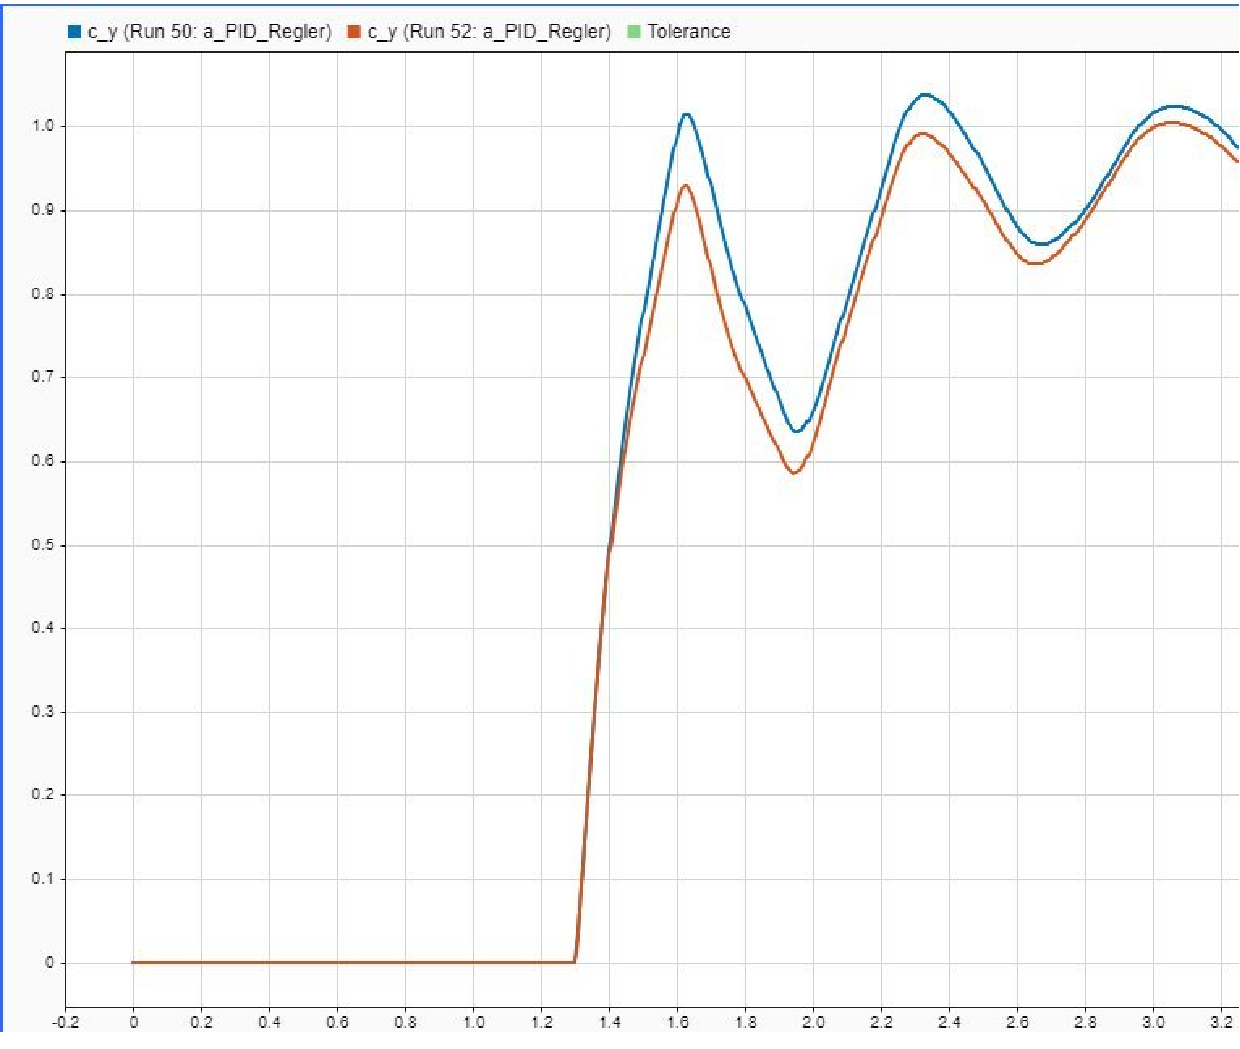
\includegraphics[width=0.8\textwidth]{Abbildungen/windup_aufgabe_7C_2.pdf}
    \caption{Windup-Effekt im Regelkreis}
    \label{fig:windup_7C2}
\end{figure}

\subsubsection{Ergebnisse}

\begin{itemize}
\item Bei der Begrenzung auf $\left[-3,3\right]$ tritt nur ein geringer Einfluss auf das Regelverhalten auf.
\item Bei der stärkeren Begrenzung auf $\left[-1.5,1.5\right]$ steigt die Einschwingzeit deutlich an und er kann den gewünschten Sollwert nicht mehr erreichen.
\item Im Bezug auf die Ausgangssprungantwort, ist das Phänomen des Windup-Effekts nicht zu beobachten (da die Ausgangssprungantwort bereits stark schwingt) aber man kann es im Kontrast zum gleichen Verlauf mit Anti-Windup-Maßnahme erkennen.
\end{itemize}

\subsection{Aufgabe D -- Einfluss eines Störsignals}
In der letzen Aufgabe, soll der Einfluss eines Störsignals auf das Regelverhalten untersucht werden. Hierbei wird ein Störsignal (verzögerte Sprungfunktion) auf die Stellgröße gegeben, um zu sehen, wie sich das System verhält.

\subsubsection{Versuchsaufbau und Durchführung}
Als Störsignal ($D$) wurde eine verzögerte Sprungfunktion ($Step time=5$) verwendet, die auf die Stellgröße wirkt.


Eine Störung am Eingang der Strecke wirkt sich anders auf das System aus, als eine Störung am Ausgang, die einem Sprung entspricht.

\begin{figure}[H]
    \centering

    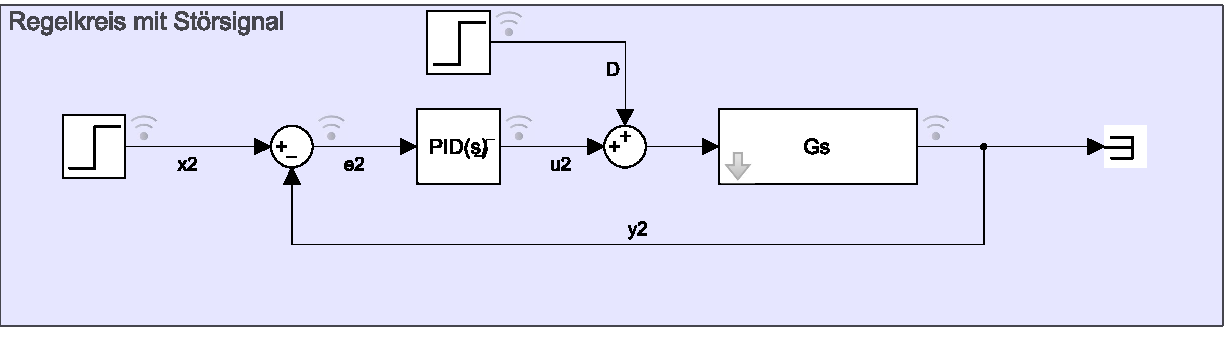
\includegraphics[width=1\textwidth]{Abbildungen/regelkreis_7_D1.pdf}
    \caption{Störsignal im Regelkreis}
    \label{fig:stelltbeschränkung_7D1}
\end{figure}

\begin{figure}[H]
    \centering

    % This file was created by matlab2tikz.
%
%The latest updates can be retrieved from
%  http://www.mathworks.com/matlabcentral/fileexchange/22022-matlab2tikz-matlab2tikz
%where you can also make suggestions and rate matlab2tikz.
%
\definecolor{mycolor1}{rgb}{0.92900,0.69400,0.12500}%
\definecolor{mycolor2}{rgb}{0.00000,0.44700,0.74100}%
\definecolor{mycolor3}{rgb}{0.12941,0.12941,0.12941}%
%
\begin{tikzpicture}

\begin{axis}[%
width=0.951\figurewidth,
height=\figureheight,
at={(0\figurewidth,0\figureheight)},
scale only axis,
xmin=-0.2,
xmax=10.2,
tick align=outside,
xlabel style={font=\color{mycolor3}},
xlabel={Time (seconds)},
ymin=-0.0674471309780858,
ymax=1.4163897505398,
axis background/.style={fill=white},
xmajorgrids,
ymajorgrids,
legend style={at={(0.144,0.935)}, anchor=south west, legend cell align=left, align=left}
]
\addplot[const plot, color=mycolor1, line width=2.0pt] table[row sep=crcr] {%
0	0\\
0.01	0\\
0.02	0\\
0.03	0\\
0.04	0\\
0.05	0\\
0.06	0\\
0.07	0\\
0.08	0\\
0.09	0\\
0.1	0\\
0.11	0\\
0.12	0\\
0.13	0\\
0.14	0\\
0.15	0\\
0.16	0\\
0.17	0\\
0.18	0\\
0.19	0\\
0.2	0\\
0.21	0\\
0.22	0\\
0.23	0\\
0.24	0\\
0.25	0\\
0.26	0\\
0.27	0\\
0.28	0\\
0.29	0\\
0.3	0\\
0.31	0\\
0.32	0\\
0.33	0\\
0.34	0\\
0.35	0\\
0.36	0\\
0.37	0\\
0.38	0\\
0.39	0\\
0.4	0\\
0.41	0\\
0.42	0\\
0.43	0\\
0.44	0\\
0.45	0\\
0.46	0\\
0.47	0\\
0.48	0\\
0.49	0\\
0.5	0\\
0.51	0\\
0.52	0\\
0.53	0\\
0.54	0\\
0.55	0\\
0.56	0\\
0.57	0\\
0.58	0\\
0.59	0\\
0.6	0\\
0.61	0\\
0.62	0\\
0.63	0\\
0.64	0\\
0.65	0\\
0.66	0\\
0.67	0\\
0.68	0\\
0.69	0\\
0.7	0\\
0.71	0\\
0.72	0\\
0.73	0\\
0.74	0\\
0.75	0\\
0.76	0\\
0.77	0\\
0.78	0\\
0.79	0\\
0.8	0\\
0.81	0\\
0.820000000000001	0\\
0.830000000000001	0\\
0.840000000000001	0\\
0.850000000000001	0\\
0.860000000000001	0\\
0.870000000000001	0\\
0.880000000000001	0\\
0.890000000000001	0\\
0.900000000000001	0\\
0.910000000000001	0\\
0.920000000000001	0\\
0.930000000000001	0\\
0.940000000000001	0\\
0.950000000000001	0\\
0.960000000000001	0\\
0.970000000000001	0\\
0.980000000000001	0\\
0.990000000000001	0\\
0.999999999999994	0\\
1	1\\
1.00706610368157	1\\
1.01413220736314	1\\
1.02274744349539	1\\
1.03274744349539	1\\
1.04274744349539	1\\
1.05274744349539	1\\
1.06274744349539	1\\
1.07274744349539	1\\
1.08154956319475	1\\
1.08154956319477	1\\
1.09154956319477	1\\
1.10154956319477	1\\
1.11154956319477	1\\
1.12154956319477	1\\
1.13154956319477	1\\
1.14154956319477	1\\
1.15154956319477	1\\
1.16154956319477	1\\
1.17154956319477	1\\
1.18154956319477	1\\
1.19154956319477	1\\
1.20154956319477	1\\
1.21154956319477	1\\
1.22154956319477	1\\
1.23154956319477	1\\
1.24154956319477	1\\
1.25154956319477	1\\
1.26154956319477	1\\
1.27154956319477	1\\
1.28154956319477	1\\
1.29154956319477	1\\
1.30154956319477	1\\
1.31072973065323	1\\
1.32007432024506	1\\
1.33007432024506	1\\
1.34007432024506	1\\
1.35007432024506	1\\
1.36007432024506	1\\
1.37007432024506	1\\
1.38007432024506	1\\
1.39007432024506	1\\
1.40007432024506	1\\
1.41007432024506	1\\
1.42007432024506	1\\
1.43007432024506	1\\
1.44007432024506	1\\
1.45007432024506	1\\
1.46007432024506	1\\
1.47007432024506	1\\
1.48007432024506	1\\
1.49007432024506	1\\
1.50007432024506	1\\
1.51007432024506	1\\
1.52007432024506	1\\
1.53007432024506	1\\
1.54007432024506	1\\
1.55007432024506	1\\
1.56007432024506	1\\
1.57007432024506	1\\
1.58007432024506	1\\
1.59007432024506	1\\
1.60007432024506	1\\
1.61007432024506	1\\
1.62007432024506	1\\
1.63007432024506	1\\
1.64007432024506	1\\
1.65007432024506	1\\
1.66007432024506	1\\
1.67007432024506	1\\
1.68007432024506	1\\
1.69007432024506	1\\
1.70007432024506	1\\
1.71007432024506	1\\
1.72007432024506	1\\
1.73007432024506	1\\
1.74007432024506	1\\
1.75007432024506	1\\
1.76007432024506	1\\
1.77007432024506	1\\
1.78007432024506	1\\
1.79007432024506	1\\
1.80007432024506	1\\
1.81007432024506	1\\
1.82007432024506	1\\
1.83007432024506	1\\
1.84007432024506	1\\
1.85007432024506	1\\
1.86007432024506	1\\
1.87007432024506	1\\
1.88007432024506	1\\
1.89007432024506	1\\
1.90007432024506	1\\
1.91007432024506	1\\
1.92007432024506	1\\
1.93007432024506	1\\
1.94007432024506	1\\
1.95007432024506	1\\
1.96007432024506	1\\
1.97007432024506	1\\
1.98007432024506	1\\
1.99007432024506	1\\
2.00007432024506	1\\
2.01007432024506	1\\
2.02007432024506	1\\
2.03007432024506	1\\
2.04007432024506	1\\
2.05007432024506	1\\
2.06007432024506	1\\
2.07007432024506	1\\
2.08007432024506	1\\
2.09007432024506	1\\
2.10007432024506	1\\
2.11007432024506	1\\
2.12007432024506	1\\
2.13007432024506	1\\
2.14007432024506	1\\
2.15007432024506	1\\
2.16007432024506	1\\
2.17007432024506	1\\
2.18007432024506	1\\
2.19007432024506	1\\
2.20007432024506	1\\
2.21007432024506	1\\
2.22007432024506	1\\
2.23007432024506	1\\
2.24007432024506	1\\
2.25007432024506	1\\
2.26007432024505	1\\
2.27007432024505	1\\
2.28007432024505	1\\
2.29007432024505	1\\
2.30007432024505	1\\
2.31007432024505	1\\
2.32007432024505	1\\
2.33007432024505	1\\
2.34007432024505	1\\
2.35007432024505	1\\
2.36007432024505	1\\
2.37007432024505	1\\
2.38007432024505	1\\
2.39007432024505	1\\
2.40007432024505	1\\
2.41007432024505	1\\
2.42007432024505	1\\
2.43007432024505	1\\
2.44007432024505	1\\
2.45007432024505	1\\
2.46007432024505	1\\
2.47007432024505	1\\
2.48007432024505	1\\
2.49007432024505	1\\
2.50007432024505	1\\
2.51007432024505	1\\
2.52007432024505	1\\
2.53007432024505	1\\
2.54007432024505	1\\
2.55007432024505	1\\
2.56007432024505	1\\
2.57007432024505	1\\
2.58007432024505	1\\
2.59007432024505	1\\
2.60007432024505	1\\
2.61007432024505	1\\
2.62007432024505	1\\
2.63007432024505	1\\
2.64007432024505	1\\
2.65007432024505	1\\
2.66007432024505	1\\
2.67007432024505	1\\
2.68007432024505	1\\
2.69007432024505	1\\
2.70007432024505	1\\
2.71007432024505	1\\
2.72007432024505	1\\
2.73007432024504	1\\
2.74007432024504	1\\
2.75007432024504	1\\
2.76007432024504	1\\
2.77007432024504	1\\
2.78007432024504	1\\
2.79007432024504	1\\
2.80007432024504	1\\
2.81007432024504	1\\
2.82007432024504	1\\
2.83007432024504	1\\
2.84007432024504	1\\
2.85007432024504	1\\
2.86007432024504	1\\
2.87007432024504	1\\
2.88007432024504	1\\
2.89007432024504	1\\
2.90007432024504	1\\
2.91007432024504	1\\
2.92007432024504	1\\
2.93007432024504	1\\
2.94007432024504	1\\
2.95007432024504	1\\
2.96007432024504	1\\
2.97007432024504	1\\
2.98007432024504	1\\
2.99007432024504	1\\
2.99965935865395	1\\
2.99965935865398	1\\
2.99965935865401	1\\
3.009659358654	1\\
3.019659358654	1\\
3.029659358654	1\\
3.039659358654	1\\
3.049659358654	1\\
3.059659358654	1\\
3.069659358654	1\\
3.079659358654	1\\
3.089659358654	1\\
3.099659358654	1\\
3.109659358654	1\\
3.11036573515563	1\\
3.11036573515565	1\\
3.12036573515565	1\\
3.13036573515565	1\\
3.14036573515565	1\\
3.15036573515565	1\\
3.16036573515565	1\\
3.17036573515565	1\\
3.18036573515565	1\\
3.19036573515565	1\\
3.20036573515565	1\\
3.21036573515565	1\\
3.22036573515565	1\\
3.23036573515565	1\\
3.24036573515565	1\\
3.25036573515565	1\\
3.26036573515565	1\\
3.27036573515565	1\\
3.28036573515565	1\\
3.29036573515565	1\\
3.30036573515565	1\\
3.31036573515565	1\\
3.32036573515565	1\\
3.33036573515565	1\\
3.34036573515565	1\\
3.35036573515565	1\\
3.36036573515565	1\\
3.37036573515565	1\\
3.38036573515565	1\\
3.39036573515565	1\\
3.40036573515565	1\\
3.41036573515565	1\\
3.42036573515565	1\\
3.43036573515565	1\\
3.44036573515565	1\\
3.45036573515565	1\\
3.46036573515565	1\\
3.47036573515565	1\\
3.48036573515565	1\\
3.49036573515565	1\\
3.50036573515565	1\\
3.51036573515565	1\\
3.52036573515565	1\\
3.53036573515565	1\\
3.54036573515565	1\\
3.55036573515565	1\\
3.56036573515564	1\\
3.57036573515564	1\\
3.58036573515564	1\\
3.59036573515564	1\\
3.60036573515564	1\\
3.61036573515564	1\\
3.62036573515564	1\\
3.63036573515564	1\\
3.64036573515564	1\\
3.65036573515564	1\\
3.66036573515564	1\\
3.67036573515564	1\\
3.68036573515564	1\\
3.69036573515564	1\\
3.69576249204826	1\\
3.69576249204829	1\\
3.69576249204832	1\\
3.70576249204832	1\\
3.71576249204832	1\\
3.72576249204832	1\\
3.73576249204832	1\\
3.74576249204832	1\\
3.75576249204832	1\\
3.76576249204832	1\\
3.77576249204832	1\\
3.78576249204832	1\\
3.79576249204832	1\\
3.80576249204832	1\\
3.81576249204832	1\\
3.82576249204832	1\\
3.83576249204831	1\\
3.84576249204831	1\\
3.85576249204831	1\\
3.86576249204831	1\\
3.87318171725598	1\\
3.87318171725601	1\\
3.87318171725604	1\\
3.88318171725604	1\\
3.89318171725604	1\\
3.90318171725604	1\\
3.91318171725604	1\\
3.92318171725604	1\\
3.93318171725604	1\\
3.94318171725604	1\\
3.95318171725604	1\\
3.96318171725604	1\\
3.97318171725604	1\\
3.98318171725604	1\\
3.99318171725604	1\\
4.00318171725604	1\\
4.01318171725604	1\\
4.02318171725604	1\\
4.03318171725603	1\\
4.04318171725603	1\\
4.05318171725603	1\\
4.06318171725603	1\\
4.07318171725603	1\\
4.08318171725603	1\\
4.09318171725603	1\\
4.10318171725603	1\\
4.11318171725603	1\\
4.12318171725603	1\\
4.13318171725603	1\\
4.14318171725603	1\\
4.15318171725603	1\\
4.16318171725603	1\\
4.17318171725603	1\\
4.18318171725603	1\\
4.19318171725603	1\\
4.20318171725603	1\\
4.21318171725603	1\\
4.22318171725603	1\\
4.23318171725603	1\\
4.24318171725603	1\\
4.25318171725603	1\\
4.26318171725603	1\\
4.27318171725603	1\\
4.28318171725603	1\\
4.29318171725603	1\\
4.30318171725603	1\\
4.31318171725603	1\\
4.32318171725603	1\\
4.33318171725603	1\\
4.34318171725603	1\\
4.35318171725603	1\\
4.36318171725603	1\\
4.37318171725603	1\\
4.38318171725603	1\\
4.39318171725603	1\\
4.40093688536439	1\\
4.40093688536444	1\\
4.4009368853645	1\\
4.4109368853645	1\\
4.4209368853645	1\\
4.4309368853645	1\\
4.4409368853645	1\\
4.4509368853645	1\\
4.4609368853645	1\\
4.4709368853645	1\\
4.4809368853645	1\\
4.4909368853645	1\\
4.5009368853645	1\\
4.5109368853645	1\\
4.5209368853645	1\\
4.5309368853645	1\\
4.5409368853645	1\\
4.5509368853645	1\\
4.5609368853645	1\\
4.5709368853645	1\\
4.5809368853645	1\\
4.5909368853645	1\\
4.6009368853645	1\\
4.6109368853645	1\\
4.61713757467801	1\\
4.61713757467806	1\\
4.61713757467812	1\\
4.62713757467812	1\\
4.63713757467812	1\\
4.64713757467812	1\\
4.65713757467812	1\\
4.66713757467812	1\\
4.67713757467812	1\\
4.68713757467812	1\\
4.69713757467812	1\\
4.70713757467812	1\\
4.71713757467812	1\\
4.72713757467812	1\\
4.73713757467812	1\\
4.74713757467812	1\\
4.75713757467812	1\\
4.76713757467812	1\\
4.77713757467812	1\\
4.78713757467812	1\\
4.79713757467812	1\\
4.80713757467812	1\\
4.81713757467812	1\\
4.82713757467812	1\\
4.83713757467812	1\\
4.84713757467812	1\\
4.85713757467812	1\\
4.86713757467812	1\\
4.87713757467812	1\\
4.88713757467812	1\\
4.89713757467812	1\\
4.90713757467812	1\\
4.91713757467812	1\\
4.92713757467811	1\\
4.93713757467811	1\\
4.94713757467811	1\\
4.95713757467811	1\\
4.96713757467811	1\\
4.97713757467811	1\\
4.98713757467811	1\\
4.99713757467811	1\\
4.99999999999994	1\\
5	1\\
5.00000000000006	1\\
5.01000000000006	1\\
5.02000000000006	1\\
5.03000000000006	1\\
5.04000000000006	1\\
5.05000000000006	1\\
5.06000000000006	1\\
5.07000000000006	1\\
5.08000000000006	1\\
5.09000000000005	1\\
5.10000000000005	1\\
5.11000000000005	1\\
5.1110177478645	1\\
5.11101774786456	1\\
5.11101774786461	1\\
5.12101774786461	1\\
5.13101774786461	1\\
5.14101774786461	1\\
5.15101774786461	1\\
5.16101774786461	1\\
5.17101774786461	1\\
5.18101774786461	1\\
5.19101774786461	1\\
5.20101774786461	1\\
5.21101774786461	1\\
5.22101774786461	1\\
5.23101774786461	1\\
5.24101774786461	1\\
5.25101774786461	1\\
5.26101774786461	1\\
5.27101774786461	1\\
5.28101774786461	1\\
5.29101774786461	1\\
5.30101774786461	1\\
5.31101774786461	1\\
5.32101774786461	1\\
5.33101774786461	1\\
5.34101774786461	1\\
5.35101774786461	1\\
5.35793741680378	1\\
5.35793741680384	1\\
5.36793741680384	1\\
5.37793741680384	1\\
5.38793741680383	1\\
5.39793741680383	1\\
5.40793741680383	1\\
5.41793741680383	1\\
5.42793741680383	1\\
5.43793741680383	1\\
5.44793741680383	1\\
5.45793741680383	1\\
5.46793741680383	1\\
5.47793741680383	1\\
5.48793741680383	1\\
5.49793741680383	1\\
5.50793741680383	1\\
5.51793741680383	1\\
5.52793741680383	1\\
5.53793741680383	1\\
5.54793741680383	1\\
5.55793741680383	1\\
5.56793741680383	1\\
5.57793741680383	1\\
5.58793741680383	1\\
5.59793741680383	1\\
5.60793741680383	1\\
5.61793741680383	1\\
5.62793741680383	1\\
5.63793741680383	1\\
5.64793741680383	1\\
5.65793741680383	1\\
5.66793741680383	1\\
5.67793741680383	1\\
5.68793741680383	1\\
5.69793741680383	1\\
5.70793741680383	1\\
5.71793741680383	1\\
5.72793741680383	1\\
5.73793741680383	1\\
5.74793741680383	1\\
5.75793741680383	1\\
5.76793741680383	1\\
5.77793741680383	1\\
5.78793741680383	1\\
5.79793741680383	1\\
5.80793741680383	1\\
5.81793741680383	1\\
5.8248425459055	1\\
5.82484254590556	1\\
5.83484254590556	1\\
5.84484254590556	1\\
5.85484254590556	1\\
5.86484254590556	1\\
5.87484254590556	1\\
5.88484254590556	1\\
5.89484254590556	1\\
5.90484254590555	1\\
5.91484254590555	1\\
5.92484254590555	1\\
5.93484254590555	1\\
5.94484254590555	1\\
5.95484254590555	1\\
5.96484254590555	1\\
5.97484254590555	1\\
5.98484254590555	1\\
5.99484254590555	1\\
6.00484254590555	1\\
6.01484254590555	1\\
6.02484254590555	1\\
6.03484254590555	1\\
6.04484254590555	1\\
6.05484254590555	1\\
6.06484254590555	1\\
6.07484254590555	1\\
6.08484254590555	1\\
6.09483166360934	1\\
6.09483166360939	1\\
6.09483166360945	1\\
6.10483166360945	1\\
6.11483166360945	1\\
6.12483166360945	1\\
6.13483166360945	1\\
6.14483166360945	1\\
6.15483166360945	1\\
6.16483166360945	1\\
6.17483166360945	1\\
6.18483166360945	1\\
6.19483166360945	1\\
6.20483166360945	1\\
6.21483166360945	1\\
6.22483166360945	1\\
6.23483166360945	1\\
6.24483166360945	1\\
6.25483166360945	1\\
6.26483166360945	1\\
6.27483166360945	1\\
6.28483166360945	1\\
6.29483166360945	1\\
6.30483166360945	1\\
6.31483166360945	1\\
6.32483166360945	1\\
6.33483166360945	1\\
6.34483166360945	1\\
6.35483166360945	1\\
6.36483166360945	1\\
6.37483166360945	1\\
6.38483166360944	1\\
6.39483166360944	1\\
6.40483166360944	1\\
6.41483166360944	1\\
6.42483166360944	1\\
6.43483166360944	1\\
6.44483166360944	1\\
6.45483166360944	1\\
6.46483166360944	1\\
6.47483166360944	1\\
6.48483166360944	1\\
6.49483166360944	1\\
6.50483166360944	1\\
6.51483166360944	1\\
6.52483166360944	1\\
6.53483166360944	1\\
6.54145864150457	1\\
6.54145864150462	1\\
6.54145864150468	1\\
6.55145864150468	1\\
6.56145864150468	1\\
6.57145864150468	1\\
6.58145864150468	1\\
6.59145864150468	1\\
6.60145864150468	1\\
6.61145864150468	1\\
6.62145864150468	1\\
6.63145864150468	1\\
6.64145864150468	1\\
6.65145864150468	1\\
6.66145864150468	1\\
6.67145864150468	1\\
6.68145864150468	1\\
6.69145864150468	1\\
6.70145864150468	1\\
6.71145864150468	1\\
6.72145864150468	1\\
6.73145864150468	1\\
6.74145864150468	1\\
6.75145864150468	1\\
6.76145864150468	1\\
6.77145864150468	1\\
6.78145864150468	1\\
6.79145864150468	1\\
6.80145864150468	1\\
6.81145864150468	1\\
6.82145864150467	1\\
6.82913773823873	1\\
6.82913773823879	1\\
6.82913773823884	1\\
6.83913773823884	1\\
6.84913773823884	1\\
6.85913773823884	1\\
6.86913773823884	1\\
6.87913773823884	1\\
6.88913773823884	1\\
6.89913773823884	1\\
6.90913773823884	1\\
6.91913773823884	1\\
6.92913773823884	1\\
6.93913773823884	1\\
6.94913773823884	1\\
6.95913773823884	1\\
6.96913773823884	1\\
6.97913773823884	1\\
6.98913773823884	1\\
6.99913773823884	1\\
7.00913773823884	1\\
7.01913773823884	1\\
7.02913773823884	1\\
7.03913773823884	1\\
7.04913773823884	1\\
7.05913773823884	1\\
7.06913773823884	1\\
7.07913773823884	1\\
7.08913773823884	1\\
7.09913773823884	1\\
7.10913773823884	1\\
7.11913773823884	1\\
7.12913773823884	1\\
7.13913773823884	1\\
7.14913773823884	1\\
7.15913773823884	1\\
7.16913773823884	1\\
7.17913773823884	1\\
7.18913773823884	1\\
7.19913773823883	1\\
7.20913773823883	1\\
7.21913773823883	1\\
7.22913773823883	1\\
7.23913773823883	1\\
7.24913773823883	1\\
7.25913773823883	1\\
7.25991904764375	1\\
7.25991904764381	1\\
7.25991904764387	1\\
7.26991904764387	1\\
7.27991904764387	1\\
7.28991904764387	1\\
7.29991904764387	1\\
7.30991904764387	1\\
7.31991904764387	1\\
7.32991904764387	1\\
7.33991904764387	1\\
7.34991904764387	1\\
7.35991904764387	1\\
7.36991904764387	1\\
7.37991904764387	1\\
7.38991904764387	1\\
7.39991904764387	1\\
7.40991904764387	1\\
7.41991904764387	1\\
7.42991904764386	1\\
7.43991904764386	1\\
7.44991904764386	1\\
7.45991904764386	1\\
7.46991904764386	1\\
7.47991904764386	1\\
7.48991904764386	1\\
7.49991904764386	1\\
7.50991904764386	1\\
7.51991904764386	1\\
7.52991904764386	1\\
7.53991904764386	1\\
7.54991904764386	1\\
7.55991904764386	1\\
7.56180893618041	1\\
7.56180893618048	1\\
7.56180893618054	1\\
7.57180893618054	1\\
7.58180893618054	1\\
7.59180893618054	1\\
7.60180893618054	1\\
7.61180893618054	1\\
7.62180893618054	1\\
7.63180893618054	1\\
7.64180893618054	1\\
7.65180893618053	1\\
7.66180893618053	1\\
7.67180893618053	1\\
7.68180893618053	1\\
7.69180893618053	1\\
7.70180893618053	1\\
7.71180893618053	1\\
7.72180893618053	1\\
7.73180893618053	1\\
7.74180893618053	1\\
7.75180893618053	1\\
7.76180893618053	1\\
7.77180893618053	1\\
7.78180893618053	1\\
7.79180893618053	1\\
7.80180893618053	1\\
7.81180893618053	1\\
7.82180893618053	1\\
7.83180893618053	1\\
7.84180893618053	1\\
7.85180893618053	1\\
7.86180893618053	1\\
7.87180893618053	1\\
7.88180893618053	1\\
7.89180893618053	1\\
7.90180893618053	1\\
7.91180893618053	1\\
7.92180893618053	1\\
7.93180893618053	1\\
7.94180893618053	1\\
7.95180893618053	1\\
7.96180893618053	1\\
7.97180893618053	1\\
7.97979617490684	1\\
7.97979617490689	1\\
7.98979617490689	1\\
7.99979617490689	1\\
8.00979617490689	1\\
8.01979617490689	1\\
8.02979617490689	1\\
8.03979617490689	1\\
8.04979617490689	1\\
8.05979617490689	1\\
8.06979617490689	1\\
8.07979617490689	1\\
8.08979617490689	1\\
8.09979617490689	1\\
8.10979617490689	1\\
8.11979617490689	1\\
8.12979617490689	1\\
8.13979617490689	1\\
8.14979617490689	1\\
8.15979617490689	1\\
8.16979617490689	1\\
8.17979617490689	1\\
8.18979617490689	1\\
8.19979617490689	1\\
8.20979617490689	1\\
8.21979617490689	1\\
8.22979617490689	1\\
8.23979617490689	1\\
8.24979617490689	1\\
8.25979617490689	1\\
8.26979617490689	1\\
8.27979617490689	1\\
8.28979617490689	1\\
8.29311406607693	1\\
8.29311406607704	1\\
8.29311406607715	1\\
8.30311406607715	1\\
8.31311406607715	1\\
8.32311406607715	1\\
8.33311406607715	1\\
8.34311406607715	1\\
8.35311406607715	1\\
8.36311406607715	1\\
8.37311406607715	1\\
8.38311406607715	1\\
8.39311406607715	1\\
8.40311406607715	1\\
8.41311406607715	1\\
8.42311406607715	1\\
8.43311406607715	1\\
8.44311406607715	1\\
8.45311406607715	1\\
8.46311406607715	1\\
8.47311406607715	1\\
8.48311406607715	1\\
8.49311406607715	1\\
8.50311406607715	1\\
8.51311406607715	1\\
8.52311406607715	1\\
8.53311406607715	1\\
8.54311406607715	1\\
8.55311406607715	1\\
8.56311406607715	1\\
8.57311406607715	1\\
8.58311406607715	1\\
8.59311406607715	1\\
8.60311406607715	1\\
8.61311406607715	1\\
8.62311406607715	1\\
8.63311406607715	1\\
8.64311406607715	1\\
8.65311406607715	1\\
8.66311406607715	1\\
8.67311406607715	1\\
8.68311406607715	1\\
8.69311406607715	1\\
8.70078598828745	1\\
8.70078598828757	1\\
8.70078598828768	1\\
8.71078598828768	1\\
8.72078598828768	1\\
8.73078598828768	1\\
8.74078598828768	1\\
8.75078598828768	1\\
8.76078598828768	1\\
8.77078598828768	1\\
8.78078598828768	1\\
8.79078598828768	1\\
8.80078598828768	1\\
8.81078598828768	1\\
8.82078598828768	1\\
8.83078598828768	1\\
8.84078598828768	1\\
8.85078598828768	1\\
8.86078598828768	1\\
8.87078598828768	1\\
8.88078598828768	1\\
8.89078598828768	1\\
8.90078598828768	1\\
8.91078598828768	1\\
8.92078598828768	1\\
8.93078598828768	1\\
8.94078598828768	1\\
8.95078598828768	1\\
8.96078598828768	1\\
8.97078598828768	1\\
8.98078598828767	1\\
8.99078598828767	1\\
9.00078598828767	1\\
9.01078598828767	1\\
9.02078598828767	1\\
9.02332854450241	1\\
9.02332854450257	1\\
9.0233285445028	1\\
9.02332854450291	1\\
9.02332854450314	1\\
9.02332854450337	1\\
9.02332854450382	1\\
9.02332854450473	1\\
9.02332854450655	1\\
9.02332854451019	1\\
9.02332854451747	1\\
9.02332854453202	1\\
9.02332854456112	1\\
9.02332854461933	1\\
9.02332854473574	1\\
9.02332854496857	1\\
9.02332854543424	1\\
9.02332854636556	1\\
9.0233285482282	1\\
9.02332855195349	1\\
9.02332855940407	1\\
9.02332857430524	1\\
9.02332860410756	1\\
9.0233286637122	1\\
9.02332878292149	1\\
9.02332902134007	1\\
9.02332949817723	1\\
9.02333045185155	1\\
9.02333235920018	1\\
9.02333617389744	1\\
9.02334380329198	1\\
9.02335906208104	1\\
9.02338957965916	1\\
9.02345061481541	1\\
9.02357268512791	1\\
9.02381682575291	1\\
9.02430510700291	1\\
9.02528166950291	1\\
9.02723479450291	1\\
9.03114104450291	1\\
9.03895354450291	1\\
9.04895354450291	1\\
9.05895354450291	1\\
9.06895354450291	1\\
9.07895354450291	1\\
9.08895354450291	1\\
9.09895354450291	1\\
9.10895354450291	1\\
9.11895354450291	1\\
9.12895354450291	1\\
9.13895354450291	1\\
9.14895354450291	1\\
9.15895354450291	1\\
9.16895354450291	1\\
9.17895354450291	1\\
9.18895354450291	1\\
9.19895354450291	1\\
9.20895354450291	1\\
9.21895354450291	1\\
9.22895354450291	1\\
9.23895354450291	1\\
9.24895354450291	1\\
9.25895354450291	1\\
9.26895354450291	1\\
9.27895354450291	1\\
9.28895354450291	1\\
9.29895354450291	1\\
9.30895354450291	1\\
9.31895354450291	1\\
9.32895354450291	1\\
9.33895354450291	1\\
9.34895354450291	1\\
9.35895354450291	1\\
9.36895354450291	1\\
9.37895354450291	1\\
9.38895354450291	1\\
9.39895354450291	1\\
9.40895354450291	1\\
9.41895354450291	1\\
9.42269546172104	1\\
9.42269546172116	1\\
9.4226954617215	1\\
9.42269546172161	1\\
9.42269546172195	1\\
9.4226954617223	1\\
9.42269546172298	1\\
9.42269546172434	1\\
9.42269546172707	1\\
9.42269546173253	1\\
9.42269546174344	1\\
9.42269546176527	1\\
9.42269546180892	1\\
9.42269546189624	1\\
9.42269546207086	1\\
9.4226954624201	1\\
9.4226954631186	1\\
9.42269546451558	1\\
9.42269546730955	1\\
9.42269547289748	1\\
9.42269548407335	1\\
9.4226955064251	1\\
9.42269555112858	1\\
9.42269564053555	1\\
9.42269581934948	1\\
9.42269617697735	1\\
9.42269689223309	1\\
9.42269832274456	1\\
9.42270118376751	1\\
9.42270690581341	1\\
9.42271834990521	1\\
9.4227412380888	1\\
9.42278701445599	1\\
9.42287856719036	1\\
9.42306167265911	1\\
9.42342788359661	1\\
9.42416030547161	1\\
9.42562514922161	1\\
9.42855483672161	1\\
9.43441421172161	1\\
9.44441421172161	1\\
9.45441421172161	1\\
9.46441421172161	1\\
9.47441421172161	1\\
9.48441421172161	1\\
9.49441421172161	1\\
9.50441421172161	1\\
9.51441421172161	1\\
9.52441421172161	1\\
9.53441421172161	1\\
9.54441421172161	1\\
9.55441421172161	1\\
9.56441421172161	1\\
9.57441421172161	1\\
9.58441421172161	1\\
9.59441421172161	1\\
9.60441421172161	1\\
9.61441421172161	1\\
9.62441421172161	1\\
9.63441421172161	1\\
9.64441421172161	1\\
9.65441421172161	1\\
9.66441421172161	1\\
9.67441421172161	1\\
9.68441421172161	1\\
9.69441421172161	1\\
9.70441421172161	1\\
9.71441421172161	1\\
9.72441421172161	1\\
9.73441421172161	1\\
9.74441421172161	1\\
9.75270423202459	1\\
9.75270423202471	1\\
9.75270423202522	1\\
9.7527042320254	1\\
9.75270423202591	1\\
9.75270423202643	1\\
9.75270423202746	1\\
9.75270423202952	1\\
9.75270423203364	1\\
9.75270423204188	1\\
9.75270423205837	1\\
9.75270423209133	1\\
9.75270423215727	1\\
9.75270423228915	1\\
9.7527042325529	1\\
9.75270423308041	1\\
9.75270423413542	1\\
9.75270423624545	1\\
9.75270424046551	1\\
9.75270424890562	1\\
9.75270426578584	1\\
9.75270429954628	1\\
9.75270436706717	1\\
9.75270450210894	1\\
9.75270477219249	1\\
9.75270531235958	1\\
9.75270639269377	1\\
9.75270855336214	1\\
9.75271287469889	1\\
9.75272151737238	1\\
9.75273880271937	1\\
9.75277337341334	1\\
9.75284251480127	1\\
9.75298079757715	1\\
9.75325736312891	1\\
9.75381049423243	1\\
9.75491675643946	1\\
9.75712928085352	1\\
9.76155432968165	1\\
9.7704044273379	1\\
9.7804044273379	1\\
9.7904044273379	1\\
9.8004044273379	1\\
9.81040442733789	1\\
9.82040442733789	1\\
9.83040442733789	1\\
9.84040442733789	1\\
9.85040442733789	1\\
9.86040442733789	1\\
9.87040442733789	1\\
9.88040442733789	1\\
9.89040442733789	1\\
9.90040442733789	1\\
9.91040442733789	1\\
9.92040442733789	1\\
9.93040442733789	1\\
9.94040442733789	1\\
9.95040442733789	1\\
9.96040442733789	1\\
9.97040442733789	1\\
9.98040442733789	1\\
9.99040442733789	1\\
10	1\\
};
\addlegendentry{x}

\addplot [color=mycolor2, line width=2.0pt]
  table[row sep=crcr]{%
0	0\\
0.01	0\\
0.02	0\\
0.03	0\\
0.04	0\\
0.05	0\\
0.06	0\\
0.07	0\\
0.08	0\\
0.09	0\\
0.1	0\\
0.11	0\\
0.12	0\\
0.13	0\\
0.14	0\\
0.15	0\\
0.16	0\\
0.17	0\\
0.18	0\\
0.19	0\\
0.2	0\\
0.21	0\\
0.22	0\\
0.23	0\\
0.24	0\\
0.25	0\\
0.26	0\\
0.27	0\\
0.28	0\\
0.29	0\\
0.3	0\\
0.31	0\\
0.32	0\\
0.33	0\\
0.34	0\\
0.35	0\\
0.36	0\\
0.37	0\\
0.38	0\\
0.39	0\\
0.4	0\\
0.41	0\\
0.42	0\\
0.43	0\\
0.44	0\\
0.45	0\\
0.46	0\\
0.47	0\\
0.48	0\\
0.49	0\\
0.5	0\\
0.51	0\\
0.52	0\\
0.53	0\\
0.54	0\\
0.55	0\\
0.56	0\\
0.57	0\\
0.58	0\\
0.59	0\\
0.6	0\\
0.61	0\\
0.62	0\\
0.63	0\\
0.64	0\\
0.65	0\\
0.66	0\\
0.67	0\\
0.68	0\\
0.69	0\\
0.7	0\\
0.71	0\\
0.72	0\\
0.73	0\\
0.74	0\\
0.75	0\\
0.76	0\\
0.77	0\\
0.78	0\\
0.79	0\\
0.8	0\\
0.81	0\\
0.820000000000001	0\\
0.830000000000001	0\\
0.840000000000001	0\\
0.850000000000001	0\\
0.860000000000001	0\\
0.870000000000001	0\\
0.880000000000001	0\\
0.890000000000001	0\\
0.900000000000001	0\\
0.910000000000001	0\\
0.920000000000001	0\\
0.930000000000001	0\\
0.940000000000001	0\\
0.950000000000001	0\\
0.960000000000001	0\\
0.970000000000001	0\\
0.980000000000001	0\\
0.990000000000001	0\\
0.999999999999994	0\\
1	0\\
1.00706610368157	0\\
1.01413220736314	0\\
1.02274744349539	0\\
1.03274744349539	0\\
1.04274744349539	0\\
1.05274744349539	0\\
1.06274744349539	0\\
1.07274744349539	0\\
1.08154956319475	0\\
1.08154956319477	0\\
1.09154956319477	0\\
1.10154956319477	0\\
1.11154956319477	0\\
1.12154956319477	0\\
1.13154956319477	0\\
1.14154956319477	0\\
1.15154956319477	0\\
1.16154956319477	0\\
1.17154956319477	0\\
1.18154956319477	0\\
1.19154956319477	0\\
1.20154956319477	0\\
1.21154956319477	0\\
1.22154956319477	0\\
1.23154956319477	0\\
1.24154956319477	0\\
1.25154956319477	0\\
1.26154956319477	0\\
1.27154956319477	0\\
1.28154956319477	0\\
1.29154956319477	0\\
1.30154956319477	0.0271467845630097\\
1.31072973065323	0.178316037703338\\
1.32007432024506	0.30301430364997\\
1.33007432024506	0.410661140866661\\
1.34007432024506	0.497744096260107\\
1.35007432024506	0.568422353629723\\
1.36007432024506	0.626357110866176\\
1.37007432024506	0.674398437982537\\
1.38007432024506	0.715030224232646\\
1.39007432024506	0.749342565536795\\
1.40007432024506	0.779119057946213\\
1.41007432024506	0.805343845382005\\
1.42007432024506	0.8288281202592\\
1.43007432024506	0.850202637773584\\
1.44007432024506	0.869957667754083\\
1.45007432024506	0.888474107659067\\
1.46007432024506	0.906047711924347\\
1.47007432024506	0.922907960377973\\
1.48007432024506	0.939232751611401\\
1.49007432024506	0.955159844876661\\
1.50007432024506	0.970795769784259\\
1.51007432024506	0.986222763971562\\
1.52007432024506	1.00150417500042\\
1.53007432024506	1.01668866624087\\
1.54007432024506	1.03181349134199\\
1.55007432024506	1.04690704335983\\
1.56007432024506	1.06199083902815\\
1.57007432024506	1.0770810631567\\
1.58007432024506	1.09218977049399\\
1.59007432024506	1.10732582085884\\
1.60007432024506	1.1223104693029\\
1.61007432024506	1.12175697287522\\
1.62007432024506	1.09992580609495\\
1.63007432024506	1.0647823370772\\
1.64007432024506	1.02346464314115\\
1.65007432024506	0.980203351147656\\
1.66007432024506	0.93764782414306\\
1.67007432024506	0.897353184056416\\
1.68007432024506	0.860118136651737\\
1.69007432024506	0.826318287055305\\
1.70007432024506	0.795932143494966\\
1.71007432024506	0.768785883407529\\
1.72007432024506	0.744599697136519\\
1.73007432024506	0.723042702068234\\
1.74007432024506	0.703769359062527\\
1.75007432024506	0.686442271213882\\
1.76007432024506	0.670745607828133\\
1.77007432024506	0.656392185742624\\
1.78007432024506	0.643126357397271\\
1.79007432024506	0.630724214498972\\
1.80007432024506	0.618992153773617\\
1.81007432024506	0.607764519668059\\
1.82007432024506	0.596900802742345\\
1.83007432024506	0.586282705853311\\
1.84007432024506	0.575811273888468\\
1.85007432024506	0.565404202666038\\
1.86007432024506	0.554993388351207\\
1.87007432024506	0.544522742823303\\
1.88007432024506	0.533946277400708\\
1.89007432024506	0.523226443245735\\
1.90007432024506	0.512346836310904\\
1.91007432024506	0.502488238967383\\
1.92007432024506	0.496799735484477\\
1.93007432024506	0.497277018731134\\
1.94007432024506	0.504162118891905\\
1.95007432024506	0.516804731988399\\
1.96007432024506	0.53413345742752\\
1.97007432024506	0.554964743711411\\
1.98007432024506	0.578177619451087\\
1.99007432024506	0.602795372091295\\
2.00007432024506	0.628021292971519\\
2.01007432024506	0.653243961818248\\
2.02007432024506	0.678018092839933\\
2.03007432024506	0.70204137275055\\
2.04007432024506	0.725128972338037\\
2.05007432024506	0.747188829048787\\
2.06007432024506	0.768199384123925\\
2.07007432024506	0.788190503265358\\
2.08007432024506	0.807227733230249\\
2.09007432024506	0.825399719221737\\
2.10007432024506	0.84280844093816\\
2.11007432024506	0.859561858566283\\
2.12007432024506	0.875768553621481\\
2.13007432024506	0.891533976880247\\
2.14007432024506	0.906957959698313\\
2.15007432024506	0.922133195154379\\
2.16007432024506	0.937144445388755\\
2.17007432024506	0.952068277721359\\
2.18007432024506	0.966973172947386\\
2.19007432024506	0.981919884058787\\
2.20007432024506	0.996960708884659\\
2.21007432024506	1.01203431397158\\
2.22007432024506	1.02671842406208\\
2.23007432024506	1.04024482446641\\
2.24007432024506	1.05181708137411\\
2.25007432024506	1.06083498090316\\
2.26007432024505	1.06696125321023\\
2.27007432024505	1.07010976067519\\
2.28007432024505	1.07039651321313\\
2.29007432024505	1.06808020527194\\
2.30007432024505	1.06350586527863\\
2.31007432024505	1.05705718668544\\
2.32007432024505	1.04912018998173\\
2.33007432024505	1.04005806471589\\
2.34007432024505	1.03019530074306\\
2.35007432024505	1.01980923620987\\
2.36007432024505	1.00912716663219\\
2.37007432024505	0.99832736520456\\
2.38007432024505	0.987542649868744\\
2.39007432024505	0.9768654293949\\
2.40007432024505	0.966353433089745\\
2.41007432024505	0.956035560896631\\
2.42007432024505	0.945917478339624\\
2.43007432024505	0.935986726068162\\
2.44007432024505	0.926217221827247\\
2.45007432024505	0.916573109768899\\
2.46007432024505	0.907011964394816\\
2.47007432024505	0.897487389766109\\
2.48007432024505	0.887951073800174\\
2.49007432024505	0.878354366484516\\
2.50007432024505	0.868649562324208\\
2.51007432024505	0.858800237235442\\
2.52007432024505	0.84881980793447\\
2.53007432024505	0.838821047879576\\
2.54007432024505	0.829026438013054\\
2.55007432024505	0.819731113725807\\
2.56007432024505	0.811249639993965\\
2.57007432024505	0.803869553486396\\
2.58007432024505	0.79781976248013\\
2.59007432024505	0.793254543496336\\
2.60007432024505	0.790250405342407\\
2.61007432024505	0.788812109604252\\
2.62007432024505	0.788884256545983\\
2.63007432024505	0.790365411612599\\
2.64007432024505	0.793122566203563\\
2.65007432024505	0.797004506316438\\
2.66007432024505	0.801853271856585\\
2.67007432024505	0.80751334915929\\
2.68007432024505	0.813838560002092\\
2.69007432024505	0.820696814761126\\
2.70007432024505	0.827973011606159\\
2.71007432024505	0.835570412463838\\
2.72007432024505	0.843410830909023\\
2.73007432024504	0.85143394379507\\
2.74007432024504	0.859595999741442\\
2.75007432024504	0.867868152378437\\
2.76007432024504	0.876234600398939\\
2.77007432024504	0.884690673638518\\
2.78007432024504	0.893240966608629\\
2.79007432024504	0.901897589005431\\
2.80007432024504	0.910678567170542\\
2.81007432024504	0.91960558610036\\
2.82007432024504	0.928697979299823\\
2.83007432024504	0.937960464388829\\
2.84007432024504	0.947368440621687\\
2.85007432024504	0.956858667379299\\
2.86007432024504	0.966329453071335\\
2.87007432024504	0.975649093993553\\
2.88007432024504	0.984669014613589\\
2.89007432024504	0.993238093425841\\
2.90007432024504	1.00121557578547\\
2.91007432024504	1.00848106067828\\
2.92007432024504	1.01494097155637\\
2.93007432024504	1.02053159035169\\
2.94007432024504	1.02521914542536\\
2.95007432024504	1.02899763650729\\
2.96007432024504	1.0318851172208\\
2.97007432024504	1.03391909802829\\
2.98007432024504	1.03515162344411\\
2.99007432024504	1.03564444898643\\
2.99965935865395	1.03547207892415\\
2.99965935865398	1.03547207892415\\
2.99965935865401	1.03547207892415\\
3.009659358654	1.03471314726148\\
3.019659358654	1.03341404568526\\
3.029659358654	1.03163753638678\\
3.039659358654	1.02944047718113\\
3.049659358654	1.02687260413208\\
3.059659358654	1.0239758393251\\
3.069659358654	1.02078403341871\\
3.079659358654	1.01732305248439\\
3.089659358654	1.01361112414545\\
3.099659358654	1.00965936780122\\
3.109659358654	1.00547251545042\\
3.11036573515563	1.00516921369142\\
3.11036573515565	1.0051692136914\\
3.12036573515565	1.00073012471218\\
3.13036573515565	0.996052302690783\\
3.14036573515565	0.991134565156448\\
3.15036573515565	0.985983075683338\\
3.16036573515565	0.980616358711717\\
3.17036573515565	0.975068522353592\\
3.18036573515565	0.969390005780574\\
3.19036573515565	0.963645897470393\\
3.20036573515565	0.957912362373318\\
3.21036573515565	0.952271937008497\\
3.22036573515565	0.946808460481972\\
3.23036573515565	0.941602286481812\\
3.24036573515565	0.936726236774151\\
3.25036573515565	0.932242562782881\\
3.26036573515565	0.928201010927787\\
3.27036573515565	0.924637954840276\\
3.28036573515565	0.92157646698327\\
3.29036573515565	0.919026854261125\\
3.30036573515565	0.916999206150389\\
3.31036573515565	0.915463352867203\\
3.32036573515565	0.914412055124258\\
3.33036573515565	0.913822798137193\\
3.34036573515565	0.913669568797757\\
3.35036573515565	0.91392459863191\\
3.36036573515565	0.914559890918683\\
3.37036573515565	0.915548502579097\\
3.38036573515565	0.916865571981641\\
3.39036573515565	0.918489099495326\\
3.40036573515565	0.920400498292391\\
3.41036573515565	0.922576245441949\\
3.42036573515565	0.925022972713903\\
3.43036573515565	0.927724286066869\\
3.44036573515565	0.930675708278815\\
3.45036573515565	0.933874192378099\\
3.46036573515565	0.937316108682475\\
3.47036573515565	0.940994956146067\\
3.48036573515565	0.944899212599631\\
3.49036573515565	0.949010703702063\\
3.50036573515565	0.953303741474623\\
3.51036573515565	0.957745122725011\\
3.52036573515565	0.96229493225891\\
3.53036573515565	0.966907990698473\\
3.54036573515565	0.971535729327522\\
3.55036573515565	0.976128260324951\\
3.56036573515564	0.980636429652879\\
3.57036573515564	0.985013679657999\\
3.58036573515564	0.989217598083233\\
3.59036573515564	0.993211088338286\\
3.60036573515564	0.996963532265688\\
3.61036573515564	1.00044896979677\\
3.62036573515564	1.00365011459734\\
3.63036573515564	1.00655479153583\\
3.64036573515564	1.00915633457342\\
3.65036573515564	1.01145285693086\\
3.66036573515564	1.01344641484146\\
3.67036573515564	1.01514212323328\\
3.68036573515564	1.01654727250543\\
3.69036573515564	1.01767048542583\\
3.69576249204826	1.01812945673222\\
3.69576249204829	1.01812945673222\\
3.69576249204832	1.01812945673222\\
3.70576249204832	1.01883771804369\\
3.71576249204832	1.01928691193403\\
3.72576249204832	1.0194846242987\\
3.73576249204832	1.01943723428719\\
3.74576249204832	1.01914973757691\\
3.75576249204832	1.01862580847995\\
3.76576249204832	1.0178682297061\\
3.77576249204832	1.01687960043767\\
3.78576249204832	1.01566324115061\\
3.79576249204832	1.01422417176867\\
3.80576249204832	1.01257002599585\\
3.81576249204832	1.01071177861047\\
3.82576249204832	1.00866419639126\\
3.83576249204831	1.00644596690515\\
3.84576249204831	1.00407950315956\\
3.85576249204831	1.00159045920705\\
3.86576249204831	0.999007018313078\\
3.87318171725598	0.997048420690248\\
3.87318171725601	0.99704842069024\\
3.87318171725604	0.997048420690233\\
3.88318171725604	0.994371583550297\\
3.89318171725604	0.991683387109634\\
3.90318171725604	0.989013516847296\\
3.91318171725604	0.986390102190586\\
3.92318171725604	0.983838998522697\\
3.93318171725604	0.981383272092906\\
3.94318171725604	0.979042973706038\\
3.95318171725604	0.976835008310092\\
3.96318171725604	0.974773156397114\\
3.97318171725604	0.9728682260254\\
3.98318171725604	0.971128310545094\\
3.99318171725604	0.969547814174411\\
4.00318171725604	0.968163766984362\\
4.01318171725604	0.966945960416665\\
4.02318171725604	0.965905685113581\\
4.03318171725603	0.965043267069351\\
4.04318171725603	0.964358680112063\\
4.05318171725603	0.963851847457073\\
4.06318171725603	0.963522850587164\\
4.07318171725603	0.963372010100751\\
4.08318171725603	0.963399821425047\\
4.09318171725603	0.963606747731403\\
4.10318171725603	0.963992892896758\\
4.11318171725603	0.964557594733299\\
4.12318171725603	0.965298989355029\\
4.13318171725603	0.966213600001315\\
4.14318171725603	0.967295998399076\\
4.15318171725603	0.968538575670699\\
4.16318171725603	0.969931445361243\\
4.17318171725603	0.971450318646366\\
4.18318171725603	0.973106847825193\\
4.19318171725603	0.974871634913091\\
4.20318171725603	0.976727274797892\\
4.21318171725603	0.978655396801317\\
4.22318171725603	0.980637123770665\\
4.23318171725603	0.98265354225017\\
4.24318171725603	0.984686131299679\\
4.25318171725603	0.986717135294781\\
4.26318171725603	0.988729870633059\\
4.27318171725603	0.990708957292999\\
4.28318171725603	0.992640471767362\\
4.29318171725603	0.99451228244861\\
4.30318171725603	0.996313076770409\\
4.31318171725603	0.998033469264543\\
4.32318171725603	0.999665640999363\\
4.33318171725603	1.00120279146044\\
4.34318171725603	1.00263913028198\\
4.35318171725603	1.00396967863935\\
4.36318171725603	1.00519007153923\\
4.37318171725603	1.0062963792658\\
4.38318171725603	1.0072849668434\\
4.39318171725603	1.00815240781213\\
4.40093688536439	1.00872865977152\\
4.40093688536444	1.00872865977152\\
4.4009368853645	1.00872865977152\\
4.4109368853645	1.00937292254386\\
4.4209368853645	1.00988773494079\\
4.4309368853645	1.01027083378893\\
4.4409368853645	1.01052061531043\\
4.4509368853645	1.01063633785959\\
4.4609368853645	1.01061831789519\\
4.4709368853645	1.01046870681015\\
4.4809368853645	1.01018909982391\\
4.4909368853645	1.00978431352678\\
4.5009368853645	1.00926033234643\\
4.5109368853645	1.00862423849237\\
4.5209368853645	1.00788437347589\\
4.5309368853645	1.00705017210546\\
4.5409368853645	1.00613195824734\\
4.5509368853645	1.00514071660157\\
4.5609368853645	1.00408785455243\\
4.5709368853645	1.00298496691111\\
4.5809368853645	1.00184361488346\\
4.5909368853645	1.00067511091723\\
4.6009368853645	0.999490383041704\\
4.6109368853645	0.99829986469359\\
4.61713757467801	0.997563620746204\\
4.61713757467806	0.997563620746197\\
4.61713757467812	0.997563620746191\\
4.62713757467812	0.996384479012155\\
4.63713757467812	0.995223716794813\\
4.64713757467812	0.994089310657474\\
4.65713757467812	0.992988580850509\\
4.66713757467812	0.991928247787998\\
4.67713757467812	0.990914504161762\\
4.68713757467812	0.989953093613765\\
4.69713757467812	0.989046657263262\\
4.70713757467812	0.988208380606761\\
4.71713757467812	0.987434896840656\\
4.72713757467812	0.986733511229161\\
4.73713757467812	0.986108480066434\\
4.74713757467812	0.985563741591123\\
4.75713757467812	0.985102844135936\\
4.76713757467812	0.984728829558278\\
4.77713757467812	0.984444154910532\\
4.78713757467812	0.984250696737923\\
4.79713757467812	0.984149516405535\\
4.80713757467812	0.984140766519596\\
4.81713757467812	0.984223700571997\\
4.82713757467812	0.984396647362162\\
4.83713757467812	0.984657014742135\\
4.84713757467812	0.985001324156419\\
4.85713757467812	0.985425273454181\\
4.86713757467812	0.985923823732739\\
4.87713757467812	0.98649130480788\\
4.88713757467812	0.987121533984504\\
4.89713757467812	0.987807941454064\\
4.90713757467812	0.98854369195673\\
4.91713757467812	0.9893175931597\\
4.92713757467811	0.990131844920819\\
4.93713757467811	0.990974434597118\\
4.94713757467811	0.991838530604539\\
4.95713757467811	0.992717498314041\\
4.96713757467811	0.993604939665338\\
4.97713757467811	0.994494714454125\\
4.98713757467811	0.995380945324235\\
4.99713757467811	0.996258119702029\\
4.99999999999994	0.996505038668143\\
5	0.996505038668148\\
5.00000000000006	0.996505038668153\\
5.01000000000006	0.997361992698942\\
5.02000000000006	0.998197750542068\\
5.03000000000006	0.999007456419172\\
5.04000000000006	0.999786363329994\\
5.05000000000006	1.00052990281993\\
5.06000000000006	1.00123369535758\\
5.07000000000006	1.00189357603321\\
5.08000000000006	1.00250563136596\\
5.09000000000005	1.0030662364345\\
5.10000000000005	1.00357210591149\\
5.11000000000005	1.00402036688213\\
5.1110177478645	1.00406167156103\\
5.11101774786456	1.00406167156103\\
5.11101774786461	1.00406167156104\\
5.12101774786461	1.00444366395873\\
5.13101774786461	1.0047636077201\\
5.14101774786461	1.00502023987911\\
5.15101774786461	1.00521289233283\\
5.16101774786461	1.00534150733076\\
5.17101774786461	1.0054066377778\\
5.18101774786461	1.00540943224953\\
5.19101774786461	1.00535160553203\\
5.20101774786461	1.00523539641223\\
5.21101774786461	1.0050636066781\\
5.22101774786461	1.00483929834354\\
5.23101774786461	1.00456573967396\\
5.24101774786461	1.00424687299655\\
5.25101774786461	1.00388666749322\\
5.26101774786461	1.00348924821681\\
5.27101774786461	1.00305884146384\\
5.28101774786461	1.00259972786316\\
5.29101774786461	1.00211620038669\\
5.30101774786461	1.00360901305194\\
5.31101774786461	1.0226161695772\\
5.32101774786461	1.04084598710238\\
5.33101774786461	1.05833263754547\\
5.34101774786461	1.07510905423922\\
5.35101774786461	1.0912069799418\\
5.35793741680378	1.10194164398409\\
5.35793741680384	1.10194164398418\\
5.36793741680384	1.1169617395308\\
5.37793741680384	1.13138314079786\\
5.38793741680383	1.14523350912238\\
5.39793741680383	1.15853945887975\\
5.40793741680383	1.17132656843572\\
5.41793741680383	1.18360795014164\\
5.42793741680383	1.19543065195166\\
5.43793741680383	1.20680499691944\\
5.44793741680383	1.21775241741746\\
5.45793741680383	1.22829329629362\\
5.46793741680383	1.23844696515364\\
5.47793741680383	1.24823170704347\\
5.48793741680383	1.25766476489518\\
5.49793741680383	1.26676235668174\\
5.50793741680383	1.27553969523873\\
5.51793741680383	1.28401100512014\\
5.52793741680383	1.29218960745837\\
5.53793741680383	1.30008792586907\\
5.54793741680383	1.30771751907594\\
5.55793741680383	1.31508914482471\\
5.56793741680383	1.32221281536805\\
5.57793741680383	1.32909784968161\\
5.58793741680383	1.33575292482095\\
5.59793741680383	1.34215173100415\\
5.60793741680383	1.34693534961525\\
5.61793741680383	1.34894261956172\\
5.62793741680383	1.34841089067272\\
5.63793741680383	1.345935049568\\
5.64793741680383	1.34197585678241\\
5.65793741680383	1.33698339528192\\
5.66793741680383	1.33102133218804\\
5.67793741680383	1.32442524111742\\
5.68793741680383	1.31735688591904\\
5.69793741680383	1.30994017325611\\
5.70793741680383	1.30226961393719\\
5.71793741680383	1.29441557455745\\
5.72793741680383	1.28643402841044\\
5.73793741680383	1.27836492285167\\
5.74793741680383	1.27023804363928\\
5.75793741680383	1.26207507186443\\
5.76793741680383	1.25389148113649\\
5.77793741680383	1.24569801780886\\
5.78793741680383	1.23750185564575\\
5.79793741680383	1.22930749590135\\
5.80793741680383	1.22111746809239\\
5.81793741680383	1.21293287529385\\
5.8248425459055	1.20728512853137\\
5.82484254590556	1.20728512853132\\
5.83484254590556	1.19910948070956\\
5.84484254590556	1.19093806630012\\
5.85484254590556	1.18276968829726\\
5.86484254590556	1.17460299828545\\
5.87484254590556	1.16643660964022\\
5.88484254590556	1.15826917910366\\
5.89484254590556	1.15010085828115\\
5.90484254590555	1.14199131440474\\
5.91484254590555	1.13420477583816\\
5.92484254590555	1.12709389077046\\
5.93484254590555	1.12089354755728\\
5.94484254590555	1.11570030635804\\
5.95484254590555	1.11151689520802\\
5.96484254590555	1.10830346943933\\
5.97484254590555	1.10597977490668\\
5.98484254590555	1.10445107257044\\
5.99484254590555	1.10362212535621\\
6.00484254590555	1.10340064592246\\
6.01484254590555	1.10370117758826\\
6.02484254590555	1.10444694776217\\
6.03484254590555	1.1055705206623\\
6.04484254590555	1.10701388321136\\
6.05484254590555	1.10872797510707\\
6.06484254590555	1.11067191584775\\
6.07484254590555	1.11281212372694\\
6.08484254590555	1.11512140473078\\
6.09483166360934	1.11757534648899\\
6.09483166360939	1.117575346489\\
6.09483166360945	1.11757534648901\\
6.10483166360945	1.12016223933937\\
6.11483166360945	1.12286642332205\\
6.12483166360945	1.12566731669512\\
6.13483166360945	1.12857984252228\\
6.14483166360945	1.13158747712333\\
6.15483166360945	1.13468703926353\\
6.16483166360945	1.13787670443172\\
6.17483166360945	1.1411557187384\\
6.18483166360945	1.14452414729345\\
6.19483166360945	1.14798258569966\\
6.20483166360945	1.151528315172\\
6.21483166360945	1.15513494567813\\
6.22483166360945	1.15872432084541\\
6.23483166360945	1.16218129821107\\
6.24483166360945	1.16538770929331\\
6.25483166360945	1.16824179069452\\
6.26483166360945	1.17066612124066\\
6.27483166360945	1.17260770377467\\
6.28483166360945	1.17403865592745\\
6.29483166360945	1.17495111938796\\
6.30483166360945	1.17535296958157\\
6.31483166360945	1.17526367878491\\
6.32483166360945	1.17471061203688\\
6.33483166360945	1.17372593694511\\
6.34483166360945	1.1723441439989\\
6.35483166360945	1.17060012323582\\
6.36483166360945	1.16852775905966\\
6.37483166360945	1.16615895679482\\
6.38483166360944	1.16352301875568\\
6.39483166360944	1.16064641743095\\
6.40483166360944	1.1575521435292\\
6.41483166360944	1.15426050900155\\
6.42483166360944	1.15078934333771\\
6.43483166360944	1.14715145798787\\
6.44483166360944	1.14335977763283\\
6.45483166360944	1.13942384781044\\
6.46483166360944	1.13535117666469\\
6.47483166360944	1.13114748661658\\
6.48483166360944	1.12681695374104\\
6.49483166360944	1.12236243753163\\
6.50483166360944	1.11778601973138\\
6.51483166360944	1.11309153230564\\
6.52483166360944	1.1082906963379\\
6.53483166360944	1.103408999363\\
6.54145864150457	1.10014667160903\\
6.54145864150462	1.100146671609\\
6.54145864150468	1.10014667160897\\
6.55145864150468	1.09522977175819\\
6.56145864150468	1.0903580970647\\
6.57145864150468	1.08558637480388\\
6.58145864150468	1.0809665683267\\
6.59145864150468	1.07654469843719\\
6.60145864150468	1.07235896238013\\
6.61145864150468	1.06843895605277\\
6.62145864150468	1.06480570650139\\
6.63145864150468	1.06147226975923\\
6.64145864150468	1.05844467953602\\
6.65145864150468	1.05572307672709\\
6.66145864150468	1.05330289266688\\
6.67145864150468	1.05117599545762\\
6.68145864150468	1.04933174054318\\
6.69145864150468	1.04775788509267\\
6.70145864150468	1.04644139052921\\
6.71145864150468	1.045369030594\\
6.72145864150468	1.04452785583317\\
6.73145864150468	1.04390565990416\\
6.74145864150468	1.04349124716323\\
6.75145864150468	1.04327449819018\\
6.76145864150468	1.04324649851028\\
6.77145864150468	1.04339961385129\\
6.78145864150468	1.04372748249044\\
6.79145864150468	1.04422497349028\\
6.80145864150468	1.04488810089799\\
6.81145864150468	1.04571376113827\\
6.82145864150467	1.04669894395047\\
6.82913773823873	1.0475625419884\\
6.82913773823879	1.0475625419884\\
6.82913773823884	1.04756254198841\\
6.83913773823884	1.04880655740043\\
6.84913773823884	1.05020464366895\\
6.85913773823884	1.05171832163114\\
6.86913773823884	1.05333104381367\\
6.87913773823884	1.05501635627538\\
6.88913773823884	1.05674493633095\\
6.89913773823884	1.05848618072724\\
6.90913773823884	1.06020972263358\\
6.91913773823884	1.06188672624532\\
6.92913773823884	1.06349088450373\\
6.93913773823884	1.06499910012464\\
6.94913773823884	1.06639186728818\\
6.95913773823884	1.06765339331808\\
6.96913773823884	1.06877151029409\\
6.97913773823884	1.06973742918089\\
6.98913773823884	1.07054538655085\\
6.99913773823884	1.07119222711248\\
7.00913773823884	1.07167695608475\\
7.01913773823884	1.0720002977786\\
7.02913773823884	1.07216427414374\\
7.03913773823884	1.07217180552197\\
7.04913773823884	1.07202636386447\\
7.05913773823884	1.07173168692099\\
7.06913773823884	1.07129153251793\\
7.07913773823884	1.07070947657754\\
7.08913773823884	1.06998875557272\\
7.09913773823884	1.06913214993558\\
7.10913773823884	1.0681419129269\\
7.11913773823884	1.06701978179065\\
7.12913773823884	1.06577904750705\\
7.13913773823884	1.06439716087301\\
7.14913773823884	1.06288839179828\\
7.15913773823884	1.06125625563882\\
7.16913773823884	1.05950651430458\\
7.17913773823884	1.05764733234\\
7.18913773823884	1.05568949607254\\
7.19913773823883	1.05364625959222\\
7.20913773823883	1.05153296496656\\
7.21913773823883	1.04936650930547\\
7.22913773823883	1.0471647339771\\
7.23913773823883	1.0449458028165\\
7.24913773823883	1.04272762201963\\
7.25913773823883	1.0405273384834\\
7.25991904764375	1.04035807559309\\
7.25991904764381	1.04035807559307\\
7.25991904764387	1.04035807559306\\
7.26991904764387	1.0381954580787\\
7.27991904764387	1.03608226344983\\
7.28991904764387	1.0340312497701\\
7.29991904764387	1.03205344855287\\
7.30991904764387	1.03015816850975\\
7.31991904764387	1.02835306758148\\
7.32991904764387	1.02664427646992\\
7.33991904764387	1.02503655956429\\
7.34991904764387	1.023533499894\\
7.35991904764387	1.02213769362696\\
7.36991904764387	1.0208509441276\\
7.37991904764387	1.01967444980101\\
7.38991904764387	1.0186089800287\\
7.39991904764387	1.0176550351006\\
7.40991904764387	1.01681298665336\\
7.41991904764387	1.01608312929602\\
7.42991904764386	1.0154652787643\\
7.43991904764386	1.01496149282197\\
7.44991904764386	1.01457127166039\\
7.45991904764386	1.014294851194\\
7.46991904764386	1.01413197894222\\
7.47991904764386	1.01408161450657\\
7.48991904764386	1.01414165972989\\
7.49991904764386	1.01430874089124\\
7.50991904764386	1.01457808017076\\
7.51991904764386	1.01494346823834\\
7.52991904764386	1.01539733521154\\
7.53991904764386	1.01593090628931\\
7.54991904764386	1.01653442164348\\
7.55991904764386	1.01719579291394\\
7.56180893618041	1.01733032558683\\
7.56180893618048	1.01733032558683\\
7.56180893618054	1.01733032558684\\
7.57180893618054	1.01804925299115\\
7.58180893618054	1.01880352080198\\
7.59180893618054	1.01958217430144\\
7.60180893618054	1.02037460928888\\
7.61180893618054	1.02117075034043\\
7.62180893618054	1.02196118545899\\
7.63180893618054	1.0227372571049\\
7.64180893618054	1.02349111198456\\
7.65180893618053	1.02421571365566\\
7.66180893618053	1.02490482335587\\
7.67180893618053	1.02555295513349\\
7.68180893618053	1.02615531123611\\
7.69180893618053	1.02670770334953\\
7.70180893618053	1.02720646484531\\
7.71180893618053	1.02764835904529\\
7.72180893618053	1.02803050269837\\
7.73180893618053	1.02835030086372\\
7.74180893618053	1.02860523143059\\
7.75180893618053	1.02879291646262\\
7.76180893618053	1.02891117972955\\
7.77180893618053	1.02895800991964\\
7.78180893618053	1.02893163975989\\
7.79180893618053	1.02883065663202\\
7.80180893618053	1.02865413058744\\
7.81180893618053	1.02840174358989\\
7.82180893618053	1.02807390379529\\
7.83180893618053	1.02767183169977\\
7.84180893618053	1.02719760936058\\
7.85180893618053	1.02665419622078\\
7.86180893618053	1.0260500742992\\
7.87180893618053	1.02538013093492\\
7.88180893618053	1.02465445291999\\
7.89180893618053	1.02387884825616\\
7.90180893618053	1.02305953961935\\
7.91180893618053	1.02220302729716\\
7.92180893618053	1.02131595519903\\
7.93180893618053	1.02040498623414\\
7.94180893618053	1.01947669185391\\
7.95180893618053	1.01853745905388\\
7.96180893618053	1.01759341669125\\
7.97180893618053	1.01665038166825\\
7.97979617490684	1.01590233107286\\
7.97979617490689	1.01590233107285\\
7.98979617490689	1.01497502744723\\
7.99979617490689	1.01406309881793\\
8.00979617490689	1.01317101051236\\
8.01979617490689	1.01230289812831\\
8.02979617490689	1.01146259211732\\
8.03979617490689	1.01065366477703\\
8.04979617490689	1.00987947787408\\
8.05979617490689	1.00914320968329\\
8.06979617490689	1.00844787540023\\
8.07979617490689	1.00779633867967\\
8.08979617490689	1.00719130580869\\
8.09979617490689	1.00663530064801\\
8.10979617490689	1.00613062220745\\
8.11979617490689	1.00567928903019\\
8.12979617490689	1.00528297620688\\
8.13979617490689	1.00494295158833\\
8.14979617490689	1.00466001761789\\
8.15979617490689	1.00443445939995\\
8.16979617490689	1.00426616353332\\
8.17979617490689	1.00415415750733\\
8.18979617490689	1.00409704681285\\
8.19979617490689	1.0040929549624\\
8.20979617490689	1.00413950797069\\
8.21979617490689	1.0042338880566\\
8.22979617490689	1.00437289665409\\
8.23979617490689	1.00455302321157\\
8.24979617490689	1.00477051628154\\
8.25979617490689	1.00502145365677\\
8.26979617490689	1.00530180873458\\
8.27979617490689	1.00560571598642\\
8.28979617490689	1.0059330232922\\
8.29311406607693	1.00604735010432\\
8.29311406607704	1.00604735010432\\
8.29311406607715	1.00604735010433\\
8.30311406607715	1.00639635395366\\
8.31311406607715	1.00675743529926\\
8.32311406607715	1.00712682181954\\
8.33311406607715	1.00750087108893\\
8.34311406607715	1.00787607477097\\
8.35311406607715	1.00824905470513\\
8.36311406607715	1.00861655482336\\
8.37311406607715	1.00897543191357\\
8.38311406607715	1.00932264679144\\
8.39311406607715	1.00965525833667\\
8.40311406607715	1.00997042296667\\
8.41311406607715	1.01026540136875\\
8.42311406607715	1.01053757332115\\
8.43311406607715	1.01078446035857\\
8.44311406607715	1.01100375503539\\
8.45311406607715	1.01119335485657\\
8.46311406607715	1.01135139506313\\
8.47311406607715	1.01147627901773\\
8.48311406607715	1.01156672409387\\
8.49311406607715	1.01162179734878\\
8.50311406607715	1.01164091184418\\
8.51311406607715	1.01162383820027\\
8.52311406607715	1.01157070688109\\
8.53311406607715	1.01148200096576\\
8.54311406607715	1.01135854028065\\
8.55311406607715	1.01120145814409\\
8.56311406607715	1.01101217224168\\
8.57311406607715	1.0107923935559\\
8.58311406607715	1.01054399688083\\
8.59311406607715	1.01027160753028\\
8.60311406607715	1.00997187432724\\
8.61311406607715	1.00965007082844\\
8.62311406607715	1.00930858912038\\
8.63311406607715	1.00894987144241\\
8.64311406607715	1.00857638718152\\
8.65311406607715	1.0081906147842\\
8.66311406607715	1.00779502851607\\
8.67311406607715	1.00739208939661\\
8.68311406607715	1.00698423947908\\
8.69311406607715	1.00657389847748\\
8.70078598828745	1.00625901442943\\
8.70078598828757	1.00625901442942\\
8.70078598828768	1.00625901442942\\
8.71078598828768	1.00585032058227\\
8.72078598828768	1.00544569171513\\
8.73078598828768	1.00504743590642\\
8.74078598828768	1.00465781599172\\
8.75078598828768	1.00427903690598\\
8.76078598828768	1.00391322958337\\
8.77078598828768	1.0035624327104\\
8.78078598828768	1.0032285718284\\
8.79078598828768	1.00291343421044\\
8.80078598828768	1.00261864582821\\
8.81078598828768	1.00234565121858\\
8.82078598828768	1.0020956956031\\
8.83078598828768	1.00186981002817\\
8.84078598828768	1.00166880040821\\
8.85078598828768	1.00149324102627\\
8.86078598828768	1.00134347272242\\
8.87078598828768	1.0012196046647\\
8.88078598828768	1.00112151270526\\
8.89078598828768	1.00104881490019\\
8.90078598828768	1.00100111300051\\
8.91078598828768	1.00097766864789\\
8.92078598828768	1.00097758644794\\
8.93078598828768	1.00099984798968\\
8.94078598828768	1.00104330823319\\
8.95078598828768	1.00110671324717\\
8.96078598828768	1.00118871669167\\
8.97078598828768	1.00128789459523\\
8.98078598828767	1.00140275817643\\
8.99078598828767	1.00153176465355\\
9.00078598828767	1.00167231916507\\
9.01078598828767	1.0018249562842\\
9.02078598828767	1.00198687006525\\
9.02332854450241	1.0020299680985\\
9.02332854450257	1.0020299680985\\
9.0233285445028	1.00202996809851\\
9.02332854450291	1.00202996809851\\
9.02332854450314	1.00202996809851\\
9.02332854450337	1.00202996809852\\
9.02332854450382	1.00202996809852\\
9.02332854450473	1.00202996809854\\
9.02332854450655	1.00202996809857\\
9.02332854451019	1.00202996809863\\
9.02332854451747	1.00202996809876\\
9.02332854453202	1.002029968099\\
9.02332854456112	1.0020299680995\\
9.02332854461933	1.00202996810048\\
9.02332854473574	1.00202996810246\\
9.02332854496857	1.0020299681064\\
9.02332854543424	1.0020299681143\\
9.02332854636556	1.00202996813008\\
9.0233285482282	1.00202996816166\\
9.02332855195349	1.0020299682248\\
9.02332855940407	1.00202996835109\\
9.02332857430524	1.00202996860368\\
9.02332860410756	1.00202996910885\\
9.0233286637122	1.00202997011919\\
9.02332878292149	1.00202997213986\\
9.02332902134007	1.00202997618122\\
9.02332949817723	1.00202998426393\\
9.02333045185155	1.00203000042935\\
9.02333235920018	1.00203003276019\\
9.02333617389744	1.00203009742186\\
9.02334380329198	1.00203022674522\\
9.02335906208104	1.00203048539193\\
9.02338957965916	1.00203100268535\\
9.02345061481541	1.00203203727218\\
9.02357268512791	1.00203410644586\\
9.02381682575291	1.00203824479321\\
9.02430510700291	1.00204652148791\\
9.02528166950291	1.00206307487731\\
9.02723479450291	1.00209618165611\\
9.03114104450291	1.00216260431222\\
9.03895354450291	1.00229963233855\\
9.04895354450291	1.00247843546089\\
9.05895354450291	1.00266000238202\\
9.06895354450291	1.00284261145706\\
9.07895354450291	1.00302455211007\\
9.08895354450291	1.0032041367106\\
9.09895354450291	1.00337971426684\\
9.10895354450291	1.00354968518565\\
9.11895354450291	1.00371251648422\\
9.12895354450291	1.00386675698987\\
9.13895354450291	1.00401105202138\\
9.14895354450291	1.00414415701857\\
9.15895354450291	1.00426494961818\\
9.16895354450291	1.00437243980793\\
9.17895354450291	1.00446577837586\\
9.18895354450291	1.0045442657074\\
9.19895354450291	1.00460734889083\\
9.20895354450291	1.00465460933683\\
9.21895354450291	1.00468578272516\\
9.22895354450291	1.00470074982944\\
9.23895354450291	1.00469952781177\\
9.24895354450291	1.00468226277954\\
9.25895354450291	1.00464922150181\\
9.26895354450291	1.00460078260994\\
9.27895354450291	1.00453742765747\\
9.28895354450291	1.00445973236688\\
9.29895354450291	1.00436841381704\\
9.30895354450291	1.00426409479431\\
9.31895354450291	1.00414763597143\\
9.32895354450291	1.0040205211038\\
9.33895354450291	1.00388261665445\\
9.34895354450291	1.00373519678644\\
9.35895354450291	1.00357948422454\\
9.36895354450291	1.0034165596261\\
9.37895354450291	1.00324754145204\\
9.38895354450291	1.00307357971163\\
9.39895354450291	1.00289584892285\\
9.40895354450291	1.0027155401709\\
9.41895354450291	1.00253385229983\\
9.42269546172104	1.00246579807004\\
9.42269546172116	1.00246579807004\\
9.4226954617215	1.00246579807004\\
9.42269546172161	1.00246579807003\\
9.42269546172195	1.00246579807003\\
9.4226954617223	1.00246579807002\\
9.42269546172298	1.00246579807001\\
9.42269546172434	1.00246579806998\\
9.42269546172707	1.00246579806993\\
9.42269546173253	1.00246579806984\\
9.42269546174344	1.00246579806964\\
9.42269546176527	1.00246579806924\\
9.42269546180892	1.00246579806845\\
9.42269546189624	1.00246579806686\\
9.42269546207086	1.00246579806368\\
9.4226954624201	1.00246579805733\\
9.4226954631186	1.00246579804463\\
9.42269546451558	1.00246579801922\\
9.42269546730955	1.00246579796841\\
9.42269547289748	1.00246579786678\\
9.42269548407335	1.00246579766352\\
9.4226955064251	1.00246579725701\\
9.42269555112858	1.00246579644399\\
9.42269564053555	1.00246579481795\\
9.42269581934948	1.00246579156586\\
9.42269617697735	1.00246578506168\\
9.42269689223309	1.00246577205333\\
9.42269832274456	1.00246574603662\\
9.42270118376751	1.00246569400321\\
9.42270690581341	1.00246558993639\\
9.42271834990521	1.00246538180275\\
9.4227412380888	1.00246496553547\\
9.42278701445599	1.00246413300091\\
9.42287856719036	1.00246246793179\\
9.42306167265911	1.00245913779354\\
9.42342788359661	1.00245247751704\\
9.42416030547161	1.00243915696406\\
9.42562514922161	1.00241251585808\\
9.42855483672161	1.00235923364612\\
9.43441421172161	1.0022532169307\\
9.44441421172161	1.00207353255945\\
9.45441421172161	1.00189663059604\\
9.46441421172161	1.00172361676984\\
9.47441421172161	1.0015555477752\\
9.48441421172161	1.00139342146527\\
9.49441421172161	1.00123816783094\\
9.50441421172161	1.00109064204511\\
9.51441421172161	1.00095161921327\\
9.52441421172161	1.00082178880072\\
9.53441421172161	1.00070175022155\\
9.54441421172161	1.00059201065465\\
9.55441421172161	1.00049298423263\\
9.56441421172161	1.00040499243333\\
9.57441421172161	1.00032826551022\\
9.58441421172161	1.00026294477415\\
9.59441421172161	1.0002090833199\\
9.60441421172161	1.00016665139761\\
9.61441421172161	1.00013554782233\\
9.62441421172161	1.00011552153538\\
9.63441421172161	1.00010637965096\\
9.64441421172161	1.00010789691685\\
9.65441421172161	1.0001196350073\\
9.66441421172161	1.00014110874949\\
9.67441421172161	1.00017181673472\\
9.68441421172161	1.00021120356223\\
9.69441421172161	1.00025866352286\\
9.70441421172161	1.00031354454691\\
9.71441421172161	1.00037515252457\\
9.72441421172161	1.00044211010247\\
9.73441421172161	1.00051503501358\\
9.74441421172161	1.00059241058455\\
9.75270423202459	1.00065956770335\\
9.75270423202471	1.00065956770335\\
9.75270423202522	1.00065956770335\\
9.7527042320254	1.00065956770336\\
9.75270423202591	1.00065956770336\\
9.75270423202643	1.00065956770336\\
9.75270423202746	1.00065956770337\\
9.75270423202952	1.00065956770339\\
9.75270423203364	1.00065956770342\\
9.75270423204188	1.00065956770349\\
9.75270423205837	1.00065956770362\\
9.75270423209133	1.00065956770389\\
9.75270423215727	1.00065956770442\\
9.75270423228915	1.00065956770549\\
9.7527042325529	1.00065956770763\\
9.75270423308041	1.0006595677119\\
9.75270423413542	1.00065956772045\\
9.75270423624545	1.00065956773754\\
9.75270424046551	1.00065956777173\\
9.75270424890562	1.0006595678401\\
9.75270426578584	1.00065956797685\\
9.75270429954628	1.00065956825034\\
9.75270436706717	1.00065956879732\\
9.75270450210894	1.00065956989129\\
9.75270477219249	1.00065957207923\\
9.75270531235958	1.0006595764551\\
9.75270639269377	1.00065958520684\\
9.75270855336214	1.00065960271033\\
9.75271287469889	1.0006596377173\\
9.75272151737238	1.00065970773125\\
9.75273880271937	1.00065984775915\\
9.75277337341334	1.00066012781494\\
9.75284251480127	1.00066068792652\\
9.75298079757715	1.00066180814969\\
9.75325736312891	1.00066404859603\\
9.75381049423243	1.0006685294887\\
9.75491675643946	1.00067763252714\\
9.75712928085352	1.00069617798464\\
9.76155432968165	1.00073326889962\\
9.7704044273379	1.00080863755769\\
9.7804044273379	1.00089512978684\\
9.7904044273379	1.00098228374976\\
9.8004044273379	1.00106928898947\\
9.81040442733789	1.00115535493581\\
9.82040442733789	1.00123971748944\\
9.83040442733789	1.00132164526352\\
9.84040442733789	1.00140044535166\\
9.85040442733789	1.00147546841422\\
9.86040442733789	1.00154611300348\\
9.87040442733789	1.00161182910079\\
9.88040442733789	1.00167212087026\\
9.89040442733789	1.00172654873009\\
9.90040442733789	1.00177473094115\\
9.91040442733789	1.00181634402005\\
9.92040442733789	1.00185112425726\\
9.93040442733789	1.00187887281101\\
9.94040442733789	1.00189943568697\\
9.95040442733789	1.00191270624248\\
9.96040442733789	1.00191864262896\\
9.97040442733789	1.00191726317655\\
9.98040442733789	1.00190863892477\\
9.99040442733789	1.00189289158382\\
10	1.00187122164471\\
};
\addlegendentry{y2}

\addplot[const plot, color=mycolor1, line width=2.0pt] table[row sep=crcr] {%
0	0\\
0.01	0\\
0.02	0\\
0.03	0\\
0.04	0\\
0.05	0\\
0.06	0\\
0.07	0\\
0.08	0\\
0.09	0\\
0.1	0\\
0.11	0\\
0.12	0\\
0.13	0\\
0.14	0\\
0.15	0\\
0.16	0\\
0.17	0\\
0.18	0\\
0.19	0\\
0.2	0\\
0.21	0\\
0.22	0\\
0.23	0\\
0.24	0\\
0.25	0\\
0.26	0\\
0.27	0\\
0.28	0\\
0.29	0\\
0.3	0\\
0.31	0\\
0.32	0\\
0.33	0\\
0.34	0\\
0.35	0\\
0.36	0\\
0.37	0\\
0.38	0\\
0.39	0\\
0.4	0\\
0.41	0\\
0.42	0\\
0.43	0\\
0.44	0\\
0.45	0\\
0.46	0\\
0.47	0\\
0.48	0\\
0.49	0\\
0.5	0\\
0.51	0\\
0.52	0\\
0.53	0\\
0.54	0\\
0.55	0\\
0.56	0\\
0.57	0\\
0.58	0\\
0.59	0\\
0.6	0\\
0.61	0\\
0.62	0\\
0.63	0\\
0.64	0\\
0.65	0\\
0.66	0\\
0.67	0\\
0.68	0\\
0.69	0\\
0.7	0\\
0.71	0\\
0.72	0\\
0.73	0\\
0.74	0\\
0.75	0\\
0.76	0\\
0.77	0\\
0.78	0\\
0.79	0\\
0.8	0\\
0.81	0\\
0.820000000000001	0\\
0.830000000000001	0\\
0.840000000000001	0\\
0.850000000000001	0\\
0.860000000000001	0\\
0.870000000000001	0\\
0.880000000000001	0\\
0.890000000000001	0\\
0.900000000000001	0\\
0.910000000000001	0\\
0.920000000000001	0\\
0.930000000000001	0\\
0.940000000000001	0\\
0.950000000000001	0\\
0.960000000000001	0\\
0.970000000000001	0\\
0.980000000000001	0\\
0.990000000000001	0\\
0.999999999999994	0\\
1	0\\
1.00706610368157	0\\
1.01413220736314	0\\
1.02274744349539	0\\
1.03274744349539	0\\
1.04274744349539	0\\
1.05274744349539	0\\
1.06274744349539	0\\
1.07274744349539	0\\
1.08154956319475	0\\
1.08154956319477	0\\
1.09154956319477	0\\
1.10154956319477	0\\
1.11154956319477	0\\
1.12154956319477	0\\
1.13154956319477	0\\
1.14154956319477	0\\
1.15154956319477	0\\
1.16154956319477	0\\
1.17154956319477	0\\
1.18154956319477	0\\
1.19154956319477	0\\
1.20154956319477	0\\
1.21154956319477	0\\
1.22154956319477	0\\
1.23154956319477	0\\
1.24154956319477	0\\
1.25154956319477	0\\
1.26154956319477	0\\
1.27154956319477	0\\
1.28154956319477	0\\
1.29154956319477	0\\
1.30154956319477	0\\
1.31072973065323	0\\
1.32007432024506	0\\
1.33007432024506	0\\
1.34007432024506	0\\
1.35007432024506	0\\
1.36007432024506	0\\
1.37007432024506	0\\
1.38007432024506	0\\
1.39007432024506	0\\
1.40007432024506	0\\
1.41007432024506	0\\
1.42007432024506	0\\
1.43007432024506	0\\
1.44007432024506	0\\
1.45007432024506	0\\
1.46007432024506	0\\
1.47007432024506	0\\
1.48007432024506	0\\
1.49007432024506	0\\
1.50007432024506	0\\
1.51007432024506	0\\
1.52007432024506	0\\
1.53007432024506	0\\
1.54007432024506	0\\
1.55007432024506	0\\
1.56007432024506	0\\
1.57007432024506	0\\
1.58007432024506	0\\
1.59007432024506	0\\
1.60007432024506	0\\
1.61007432024506	0\\
1.62007432024506	0\\
1.63007432024506	0\\
1.64007432024506	0\\
1.65007432024506	0\\
1.66007432024506	0\\
1.67007432024506	0\\
1.68007432024506	0\\
1.69007432024506	0\\
1.70007432024506	0\\
1.71007432024506	0\\
1.72007432024506	0\\
1.73007432024506	0\\
1.74007432024506	0\\
1.75007432024506	0\\
1.76007432024506	0\\
1.77007432024506	0\\
1.78007432024506	0\\
1.79007432024506	0\\
1.80007432024506	0\\
1.81007432024506	0\\
1.82007432024506	0\\
1.83007432024506	0\\
1.84007432024506	0\\
1.85007432024506	0\\
1.86007432024506	0\\
1.87007432024506	0\\
1.88007432024506	0\\
1.89007432024506	0\\
1.90007432024506	0\\
1.91007432024506	0\\
1.92007432024506	0\\
1.93007432024506	0\\
1.94007432024506	0\\
1.95007432024506	0\\
1.96007432024506	0\\
1.97007432024506	0\\
1.98007432024506	0\\
1.99007432024506	0\\
2.00007432024506	0\\
2.01007432024506	0\\
2.02007432024506	0\\
2.03007432024506	0\\
2.04007432024506	0\\
2.05007432024506	0\\
2.06007432024506	0\\
2.07007432024506	0\\
2.08007432024506	0\\
2.09007432024506	0\\
2.10007432024506	0\\
2.11007432024506	0\\
2.12007432024506	0\\
2.13007432024506	0\\
2.14007432024506	0\\
2.15007432024506	0\\
2.16007432024506	0\\
2.17007432024506	0\\
2.18007432024506	0\\
2.19007432024506	0\\
2.20007432024506	0\\
2.21007432024506	0\\
2.22007432024506	0\\
2.23007432024506	0\\
2.24007432024506	0\\
2.25007432024506	0\\
2.26007432024505	0\\
2.27007432024505	0\\
2.28007432024505	0\\
2.29007432024505	0\\
2.30007432024505	0\\
2.31007432024505	0\\
2.32007432024505	0\\
2.33007432024505	0\\
2.34007432024505	0\\
2.35007432024505	0\\
2.36007432024505	0\\
2.37007432024505	0\\
2.38007432024505	0\\
2.39007432024505	0\\
2.40007432024505	0\\
2.41007432024505	0\\
2.42007432024505	0\\
2.43007432024505	0\\
2.44007432024505	0\\
2.45007432024505	0\\
2.46007432024505	0\\
2.47007432024505	0\\
2.48007432024505	0\\
2.49007432024505	0\\
2.50007432024505	0\\
2.51007432024505	0\\
2.52007432024505	0\\
2.53007432024505	0\\
2.54007432024505	0\\
2.55007432024505	0\\
2.56007432024505	0\\
2.57007432024505	0\\
2.58007432024505	0\\
2.59007432024505	0\\
2.60007432024505	0\\
2.61007432024505	0\\
2.62007432024505	0\\
2.63007432024505	0\\
2.64007432024505	0\\
2.65007432024505	0\\
2.66007432024505	0\\
2.67007432024505	0\\
2.68007432024505	0\\
2.69007432024505	0\\
2.70007432024505	0\\
2.71007432024505	0\\
2.72007432024505	0\\
2.73007432024504	0\\
2.74007432024504	0\\
2.75007432024504	0\\
2.76007432024504	0\\
2.77007432024504	0\\
2.78007432024504	0\\
2.79007432024504	0\\
2.80007432024504	0\\
2.81007432024504	0\\
2.82007432024504	0\\
2.83007432024504	0\\
2.84007432024504	0\\
2.85007432024504	0\\
2.86007432024504	0\\
2.87007432024504	0\\
2.88007432024504	0\\
2.89007432024504	0\\
2.90007432024504	0\\
2.91007432024504	0\\
2.92007432024504	0\\
2.93007432024504	0\\
2.94007432024504	0\\
2.95007432024504	0\\
2.96007432024504	0\\
2.97007432024504	0\\
2.98007432024504	0\\
2.99007432024504	0\\
2.99965935865395	0\\
2.99965935865398	0\\
2.99965935865401	0\\
3.009659358654	0\\
3.019659358654	0\\
3.029659358654	0\\
3.039659358654	0\\
3.049659358654	0\\
3.059659358654	0\\
3.069659358654	0\\
3.079659358654	0\\
3.089659358654	0\\
3.099659358654	0\\
3.109659358654	0\\
3.11036573515563	0\\
3.11036573515565	0\\
3.12036573515565	0\\
3.13036573515565	0\\
3.14036573515565	0\\
3.15036573515565	0\\
3.16036573515565	0\\
3.17036573515565	0\\
3.18036573515565	0\\
3.19036573515565	0\\
3.20036573515565	0\\
3.21036573515565	0\\
3.22036573515565	0\\
3.23036573515565	0\\
3.24036573515565	0\\
3.25036573515565	0\\
3.26036573515565	0\\
3.27036573515565	0\\
3.28036573515565	0\\
3.29036573515565	0\\
3.30036573515565	0\\
3.31036573515565	0\\
3.32036573515565	0\\
3.33036573515565	0\\
3.34036573515565	0\\
3.35036573515565	0\\
3.36036573515565	0\\
3.37036573515565	0\\
3.38036573515565	0\\
3.39036573515565	0\\
3.40036573515565	0\\
3.41036573515565	0\\
3.42036573515565	0\\
3.43036573515565	0\\
3.44036573515565	0\\
3.45036573515565	0\\
3.46036573515565	0\\
3.47036573515565	0\\
3.48036573515565	0\\
3.49036573515565	0\\
3.50036573515565	0\\
3.51036573515565	0\\
3.52036573515565	0\\
3.53036573515565	0\\
3.54036573515565	0\\
3.55036573515565	0\\
3.56036573515564	0\\
3.57036573515564	0\\
3.58036573515564	0\\
3.59036573515564	0\\
3.60036573515564	0\\
3.61036573515564	0\\
3.62036573515564	0\\
3.63036573515564	0\\
3.64036573515564	0\\
3.65036573515564	0\\
3.66036573515564	0\\
3.67036573515564	0\\
3.68036573515564	0\\
3.69036573515564	0\\
3.69576249204826	0\\
3.69576249204829	0\\
3.69576249204832	0\\
3.70576249204832	0\\
3.71576249204832	0\\
3.72576249204832	0\\
3.73576249204832	0\\
3.74576249204832	0\\
3.75576249204832	0\\
3.76576249204832	0\\
3.77576249204832	0\\
3.78576249204832	0\\
3.79576249204832	0\\
3.80576249204832	0\\
3.81576249204832	0\\
3.82576249204832	0\\
3.83576249204831	0\\
3.84576249204831	0\\
3.85576249204831	0\\
3.86576249204831	0\\
3.87318171725598	0\\
3.87318171725601	0\\
3.87318171725604	0\\
3.88318171725604	0\\
3.89318171725604	0\\
3.90318171725604	0\\
3.91318171725604	0\\
3.92318171725604	0\\
3.93318171725604	0\\
3.94318171725604	0\\
3.95318171725604	0\\
3.96318171725604	0\\
3.97318171725604	0\\
3.98318171725604	0\\
3.99318171725604	0\\
4.00318171725604	0\\
4.01318171725604	0\\
4.02318171725604	0\\
4.03318171725603	0\\
4.04318171725603	0\\
4.05318171725603	0\\
4.06318171725603	0\\
4.07318171725603	0\\
4.08318171725603	0\\
4.09318171725603	0\\
4.10318171725603	0\\
4.11318171725603	0\\
4.12318171725603	0\\
4.13318171725603	0\\
4.14318171725603	0\\
4.15318171725603	0\\
4.16318171725603	0\\
4.17318171725603	0\\
4.18318171725603	0\\
4.19318171725603	0\\
4.20318171725603	0\\
4.21318171725603	0\\
4.22318171725603	0\\
4.23318171725603	0\\
4.24318171725603	0\\
4.25318171725603	0\\
4.26318171725603	0\\
4.27318171725603	0\\
4.28318171725603	0\\
4.29318171725603	0\\
4.30318171725603	0\\
4.31318171725603	0\\
4.32318171725603	0\\
4.33318171725603	0\\
4.34318171725603	0\\
4.35318171725603	0\\
4.36318171725603	0\\
4.37318171725603	0\\
4.38318171725603	0\\
4.39318171725603	0\\
4.40093688536439	0\\
4.40093688536444	0\\
4.4009368853645	0\\
4.4109368853645	0\\
4.4209368853645	0\\
4.4309368853645	0\\
4.4409368853645	0\\
4.4509368853645	0\\
4.4609368853645	0\\
4.4709368853645	0\\
4.4809368853645	0\\
4.4909368853645	0\\
4.5009368853645	0\\
4.5109368853645	0\\
4.5209368853645	0\\
4.5309368853645	0\\
4.5409368853645	0\\
4.5509368853645	0\\
4.5609368853645	0\\
4.5709368853645	0\\
4.5809368853645	0\\
4.5909368853645	0\\
4.6009368853645	0\\
4.6109368853645	0\\
4.61713757467801	0\\
4.61713757467806	0\\
4.61713757467812	0\\
4.62713757467812	0\\
4.63713757467812	0\\
4.64713757467812	0\\
4.65713757467812	0\\
4.66713757467812	0\\
4.67713757467812	0\\
4.68713757467812	0\\
4.69713757467812	0\\
4.70713757467812	0\\
4.71713757467812	0\\
4.72713757467812	0\\
4.73713757467812	0\\
4.74713757467812	0\\
4.75713757467812	0\\
4.76713757467812	0\\
4.77713757467812	0\\
4.78713757467812	0\\
4.79713757467812	0\\
4.80713757467812	0\\
4.81713757467812	0\\
4.82713757467812	0\\
4.83713757467812	0\\
4.84713757467812	0\\
4.85713757467812	0\\
4.86713757467812	0\\
4.87713757467812	0\\
4.88713757467812	0\\
4.89713757467812	0\\
4.90713757467812	0\\
4.91713757467812	0\\
4.92713757467811	0\\
4.93713757467811	0\\
4.94713757467811	0\\
4.95713757467811	0\\
4.96713757467811	0\\
4.97713757467811	0\\
4.98713757467811	0\\
4.99713757467811	0\\
4.99999999999994	0\\
5	1\\
5.00000000000006	1\\
5.01000000000006	1\\
5.02000000000006	1\\
5.03000000000006	1\\
5.04000000000006	1\\
5.05000000000006	1\\
5.06000000000006	1\\
5.07000000000006	1\\
5.08000000000006	1\\
5.09000000000005	1\\
5.10000000000005	1\\
5.11000000000005	1\\
5.1110177478645	1\\
5.11101774786456	1\\
5.11101774786461	1\\
5.12101774786461	1\\
5.13101774786461	1\\
5.14101774786461	1\\
5.15101774786461	1\\
5.16101774786461	1\\
5.17101774786461	1\\
5.18101774786461	1\\
5.19101774786461	1\\
5.20101774786461	1\\
5.21101774786461	1\\
5.22101774786461	1\\
5.23101774786461	1\\
5.24101774786461	1\\
5.25101774786461	1\\
5.26101774786461	1\\
5.27101774786461	1\\
5.28101774786461	1\\
5.29101774786461	1\\
5.30101774786461	1\\
5.31101774786461	1\\
5.32101774786461	1\\
5.33101774786461	1\\
5.34101774786461	1\\
5.35101774786461	1\\
5.35793741680378	1\\
5.35793741680384	1\\
5.36793741680384	1\\
5.37793741680384	1\\
5.38793741680383	1\\
5.39793741680383	1\\
5.40793741680383	1\\
5.41793741680383	1\\
5.42793741680383	1\\
5.43793741680383	1\\
5.44793741680383	1\\
5.45793741680383	1\\
5.46793741680383	1\\
5.47793741680383	1\\
5.48793741680383	1\\
5.49793741680383	1\\
5.50793741680383	1\\
5.51793741680383	1\\
5.52793741680383	1\\
5.53793741680383	1\\
5.54793741680383	1\\
5.55793741680383	1\\
5.56793741680383	1\\
5.57793741680383	1\\
5.58793741680383	1\\
5.59793741680383	1\\
5.60793741680383	1\\
5.61793741680383	1\\
5.62793741680383	1\\
5.63793741680383	1\\
5.64793741680383	1\\
5.65793741680383	1\\
5.66793741680383	1\\
5.67793741680383	1\\
5.68793741680383	1\\
5.69793741680383	1\\
5.70793741680383	1\\
5.71793741680383	1\\
5.72793741680383	1\\
5.73793741680383	1\\
5.74793741680383	1\\
5.75793741680383	1\\
5.76793741680383	1\\
5.77793741680383	1\\
5.78793741680383	1\\
5.79793741680383	1\\
5.80793741680383	1\\
5.81793741680383	1\\
5.8248425459055	1\\
5.82484254590556	1\\
5.83484254590556	1\\
5.84484254590556	1\\
5.85484254590556	1\\
5.86484254590556	1\\
5.87484254590556	1\\
5.88484254590556	1\\
5.89484254590556	1\\
5.90484254590555	1\\
5.91484254590555	1\\
5.92484254590555	1\\
5.93484254590555	1\\
5.94484254590555	1\\
5.95484254590555	1\\
5.96484254590555	1\\
5.97484254590555	1\\
5.98484254590555	1\\
5.99484254590555	1\\
6.00484254590555	1\\
6.01484254590555	1\\
6.02484254590555	1\\
6.03484254590555	1\\
6.04484254590555	1\\
6.05484254590555	1\\
6.06484254590555	1\\
6.07484254590555	1\\
6.08484254590555	1\\
6.09483166360934	1\\
6.09483166360939	1\\
6.09483166360945	1\\
6.10483166360945	1\\
6.11483166360945	1\\
6.12483166360945	1\\
6.13483166360945	1\\
6.14483166360945	1\\
6.15483166360945	1\\
6.16483166360945	1\\
6.17483166360945	1\\
6.18483166360945	1\\
6.19483166360945	1\\
6.20483166360945	1\\
6.21483166360945	1\\
6.22483166360945	1\\
6.23483166360945	1\\
6.24483166360945	1\\
6.25483166360945	1\\
6.26483166360945	1\\
6.27483166360945	1\\
6.28483166360945	1\\
6.29483166360945	1\\
6.30483166360945	1\\
6.31483166360945	1\\
6.32483166360945	1\\
6.33483166360945	1\\
6.34483166360945	1\\
6.35483166360945	1\\
6.36483166360945	1\\
6.37483166360945	1\\
6.38483166360944	1\\
6.39483166360944	1\\
6.40483166360944	1\\
6.41483166360944	1\\
6.42483166360944	1\\
6.43483166360944	1\\
6.44483166360944	1\\
6.45483166360944	1\\
6.46483166360944	1\\
6.47483166360944	1\\
6.48483166360944	1\\
6.49483166360944	1\\
6.50483166360944	1\\
6.51483166360944	1\\
6.52483166360944	1\\
6.53483166360944	1\\
6.54145864150457	1\\
6.54145864150462	1\\
6.54145864150468	1\\
6.55145864150468	1\\
6.56145864150468	1\\
6.57145864150468	1\\
6.58145864150468	1\\
6.59145864150468	1\\
6.60145864150468	1\\
6.61145864150468	1\\
6.62145864150468	1\\
6.63145864150468	1\\
6.64145864150468	1\\
6.65145864150468	1\\
6.66145864150468	1\\
6.67145864150468	1\\
6.68145864150468	1\\
6.69145864150468	1\\
6.70145864150468	1\\
6.71145864150468	1\\
6.72145864150468	1\\
6.73145864150468	1\\
6.74145864150468	1\\
6.75145864150468	1\\
6.76145864150468	1\\
6.77145864150468	1\\
6.78145864150468	1\\
6.79145864150468	1\\
6.80145864150468	1\\
6.81145864150468	1\\
6.82145864150467	1\\
6.82913773823873	1\\
6.82913773823879	1\\
6.82913773823884	1\\
6.83913773823884	1\\
6.84913773823884	1\\
6.85913773823884	1\\
6.86913773823884	1\\
6.87913773823884	1\\
6.88913773823884	1\\
6.89913773823884	1\\
6.90913773823884	1\\
6.91913773823884	1\\
6.92913773823884	1\\
6.93913773823884	1\\
6.94913773823884	1\\
6.95913773823884	1\\
6.96913773823884	1\\
6.97913773823884	1\\
6.98913773823884	1\\
6.99913773823884	1\\
7.00913773823884	1\\
7.01913773823884	1\\
7.02913773823884	1\\
7.03913773823884	1\\
7.04913773823884	1\\
7.05913773823884	1\\
7.06913773823884	1\\
7.07913773823884	1\\
7.08913773823884	1\\
7.09913773823884	1\\
7.10913773823884	1\\
7.11913773823884	1\\
7.12913773823884	1\\
7.13913773823884	1\\
7.14913773823884	1\\
7.15913773823884	1\\
7.16913773823884	1\\
7.17913773823884	1\\
7.18913773823884	1\\
7.19913773823883	1\\
7.20913773823883	1\\
7.21913773823883	1\\
7.22913773823883	1\\
7.23913773823883	1\\
7.24913773823883	1\\
7.25913773823883	1\\
7.25991904764375	1\\
7.25991904764381	1\\
7.25991904764387	1\\
7.26991904764387	1\\
7.27991904764387	1\\
7.28991904764387	1\\
7.29991904764387	1\\
7.30991904764387	1\\
7.31991904764387	1\\
7.32991904764387	1\\
7.33991904764387	1\\
7.34991904764387	1\\
7.35991904764387	1\\
7.36991904764387	1\\
7.37991904764387	1\\
7.38991904764387	1\\
7.39991904764387	1\\
7.40991904764387	1\\
7.41991904764387	1\\
7.42991904764386	1\\
7.43991904764386	1\\
7.44991904764386	1\\
7.45991904764386	1\\
7.46991904764386	1\\
7.47991904764386	1\\
7.48991904764386	1\\
7.49991904764386	1\\
7.50991904764386	1\\
7.51991904764386	1\\
7.52991904764386	1\\
7.53991904764386	1\\
7.54991904764386	1\\
7.55991904764386	1\\
7.56180893618041	1\\
7.56180893618048	1\\
7.56180893618054	1\\
7.57180893618054	1\\
7.58180893618054	1\\
7.59180893618054	1\\
7.60180893618054	1\\
7.61180893618054	1\\
7.62180893618054	1\\
7.63180893618054	1\\
7.64180893618054	1\\
7.65180893618053	1\\
7.66180893618053	1\\
7.67180893618053	1\\
7.68180893618053	1\\
7.69180893618053	1\\
7.70180893618053	1\\
7.71180893618053	1\\
7.72180893618053	1\\
7.73180893618053	1\\
7.74180893618053	1\\
7.75180893618053	1\\
7.76180893618053	1\\
7.77180893618053	1\\
7.78180893618053	1\\
7.79180893618053	1\\
7.80180893618053	1\\
7.81180893618053	1\\
7.82180893618053	1\\
7.83180893618053	1\\
7.84180893618053	1\\
7.85180893618053	1\\
7.86180893618053	1\\
7.87180893618053	1\\
7.88180893618053	1\\
7.89180893618053	1\\
7.90180893618053	1\\
7.91180893618053	1\\
7.92180893618053	1\\
7.93180893618053	1\\
7.94180893618053	1\\
7.95180893618053	1\\
7.96180893618053	1\\
7.97180893618053	1\\
7.97979617490684	1\\
7.97979617490689	1\\
7.98979617490689	1\\
7.99979617490689	1\\
8.00979617490689	1\\
8.01979617490689	1\\
8.02979617490689	1\\
8.03979617490689	1\\
8.04979617490689	1\\
8.05979617490689	1\\
8.06979617490689	1\\
8.07979617490689	1\\
8.08979617490689	1\\
8.09979617490689	1\\
8.10979617490689	1\\
8.11979617490689	1\\
8.12979617490689	1\\
8.13979617490689	1\\
8.14979617490689	1\\
8.15979617490689	1\\
8.16979617490689	1\\
8.17979617490689	1\\
8.18979617490689	1\\
8.19979617490689	1\\
8.20979617490689	1\\
8.21979617490689	1\\
8.22979617490689	1\\
8.23979617490689	1\\
8.24979617490689	1\\
8.25979617490689	1\\
8.26979617490689	1\\
8.27979617490689	1\\
8.28979617490689	1\\
8.29311406607693	1\\
8.29311406607704	1\\
8.29311406607715	1\\
8.30311406607715	1\\
8.31311406607715	1\\
8.32311406607715	1\\
8.33311406607715	1\\
8.34311406607715	1\\
8.35311406607715	1\\
8.36311406607715	1\\
8.37311406607715	1\\
8.38311406607715	1\\
8.39311406607715	1\\
8.40311406607715	1\\
8.41311406607715	1\\
8.42311406607715	1\\
8.43311406607715	1\\
8.44311406607715	1\\
8.45311406607715	1\\
8.46311406607715	1\\
8.47311406607715	1\\
8.48311406607715	1\\
8.49311406607715	1\\
8.50311406607715	1\\
8.51311406607715	1\\
8.52311406607715	1\\
8.53311406607715	1\\
8.54311406607715	1\\
8.55311406607715	1\\
8.56311406607715	1\\
8.57311406607715	1\\
8.58311406607715	1\\
8.59311406607715	1\\
8.60311406607715	1\\
8.61311406607715	1\\
8.62311406607715	1\\
8.63311406607715	1\\
8.64311406607715	1\\
8.65311406607715	1\\
8.66311406607715	1\\
8.67311406607715	1\\
8.68311406607715	1\\
8.69311406607715	1\\
8.70078598828745	1\\
8.70078598828757	1\\
8.70078598828768	1\\
8.71078598828768	1\\
8.72078598828768	1\\
8.73078598828768	1\\
8.74078598828768	1\\
8.75078598828768	1\\
8.76078598828768	1\\
8.77078598828768	1\\
8.78078598828768	1\\
8.79078598828768	1\\
8.80078598828768	1\\
8.81078598828768	1\\
8.82078598828768	1\\
8.83078598828768	1\\
8.84078598828768	1\\
8.85078598828768	1\\
8.86078598828768	1\\
8.87078598828768	1\\
8.88078598828768	1\\
8.89078598828768	1\\
8.90078598828768	1\\
8.91078598828768	1\\
8.92078598828768	1\\
8.93078598828768	1\\
8.94078598828768	1\\
8.95078598828768	1\\
8.96078598828768	1\\
8.97078598828768	1\\
8.98078598828767	1\\
8.99078598828767	1\\
9.00078598828767	1\\
9.01078598828767	1\\
9.02078598828767	1\\
9.02332854450241	1\\
9.02332854450257	1\\
9.0233285445028	1\\
9.02332854450291	1\\
9.02332854450314	1\\
9.02332854450337	1\\
9.02332854450382	1\\
9.02332854450473	1\\
9.02332854450655	1\\
9.02332854451019	1\\
9.02332854451747	1\\
9.02332854453202	1\\
9.02332854456112	1\\
9.02332854461933	1\\
9.02332854473574	1\\
9.02332854496857	1\\
9.02332854543424	1\\
9.02332854636556	1\\
9.0233285482282	1\\
9.02332855195349	1\\
9.02332855940407	1\\
9.02332857430524	1\\
9.02332860410756	1\\
9.0233286637122	1\\
9.02332878292149	1\\
9.02332902134007	1\\
9.02332949817723	1\\
9.02333045185155	1\\
9.02333235920018	1\\
9.02333617389744	1\\
9.02334380329198	1\\
9.02335906208104	1\\
9.02338957965916	1\\
9.02345061481541	1\\
9.02357268512791	1\\
9.02381682575291	1\\
9.02430510700291	1\\
9.02528166950291	1\\
9.02723479450291	1\\
9.03114104450291	1\\
9.03895354450291	1\\
9.04895354450291	1\\
9.05895354450291	1\\
9.06895354450291	1\\
9.07895354450291	1\\
9.08895354450291	1\\
9.09895354450291	1\\
9.10895354450291	1\\
9.11895354450291	1\\
9.12895354450291	1\\
9.13895354450291	1\\
9.14895354450291	1\\
9.15895354450291	1\\
9.16895354450291	1\\
9.17895354450291	1\\
9.18895354450291	1\\
9.19895354450291	1\\
9.20895354450291	1\\
9.21895354450291	1\\
9.22895354450291	1\\
9.23895354450291	1\\
9.24895354450291	1\\
9.25895354450291	1\\
9.26895354450291	1\\
9.27895354450291	1\\
9.28895354450291	1\\
9.29895354450291	1\\
9.30895354450291	1\\
9.31895354450291	1\\
9.32895354450291	1\\
9.33895354450291	1\\
9.34895354450291	1\\
9.35895354450291	1\\
9.36895354450291	1\\
9.37895354450291	1\\
9.38895354450291	1\\
9.39895354450291	1\\
9.40895354450291	1\\
9.41895354450291	1\\
9.42269546172104	1\\
9.42269546172116	1\\
9.4226954617215	1\\
9.42269546172161	1\\
9.42269546172195	1\\
9.4226954617223	1\\
9.42269546172298	1\\
9.42269546172434	1\\
9.42269546172707	1\\
9.42269546173253	1\\
9.42269546174344	1\\
9.42269546176527	1\\
9.42269546180892	1\\
9.42269546189624	1\\
9.42269546207086	1\\
9.4226954624201	1\\
9.4226954631186	1\\
9.42269546451558	1\\
9.42269546730955	1\\
9.42269547289748	1\\
9.42269548407335	1\\
9.4226955064251	1\\
9.42269555112858	1\\
9.42269564053555	1\\
9.42269581934948	1\\
9.42269617697735	1\\
9.42269689223309	1\\
9.42269832274456	1\\
9.42270118376751	1\\
9.42270690581341	1\\
9.42271834990521	1\\
9.4227412380888	1\\
9.42278701445599	1\\
9.42287856719036	1\\
9.42306167265911	1\\
9.42342788359661	1\\
9.42416030547161	1\\
9.42562514922161	1\\
9.42855483672161	1\\
9.43441421172161	1\\
9.44441421172161	1\\
9.45441421172161	1\\
9.46441421172161	1\\
9.47441421172161	1\\
9.48441421172161	1\\
9.49441421172161	1\\
9.50441421172161	1\\
9.51441421172161	1\\
9.52441421172161	1\\
9.53441421172161	1\\
9.54441421172161	1\\
9.55441421172161	1\\
9.56441421172161	1\\
9.57441421172161	1\\
9.58441421172161	1\\
9.59441421172161	1\\
9.60441421172161	1\\
9.61441421172161	1\\
9.62441421172161	1\\
9.63441421172161	1\\
9.64441421172161	1\\
9.65441421172161	1\\
9.66441421172161	1\\
9.67441421172161	1\\
9.68441421172161	1\\
9.69441421172161	1\\
9.70441421172161	1\\
9.71441421172161	1\\
9.72441421172161	1\\
9.73441421172161	1\\
9.74441421172161	1\\
9.75270423202459	1\\
9.75270423202471	1\\
9.75270423202522	1\\
9.7527042320254	1\\
9.75270423202591	1\\
9.75270423202643	1\\
9.75270423202746	1\\
9.75270423202952	1\\
9.75270423203364	1\\
9.75270423204188	1\\
9.75270423205837	1\\
9.75270423209133	1\\
9.75270423215727	1\\
9.75270423228915	1\\
9.7527042325529	1\\
9.75270423308041	1\\
9.75270423413542	1\\
9.75270423624545	1\\
9.75270424046551	1\\
9.75270424890562	1\\
9.75270426578584	1\\
9.75270429954628	1\\
9.75270436706717	1\\
9.75270450210894	1\\
9.75270477219249	1\\
9.75270531235958	1\\
9.75270639269377	1\\
9.75270855336214	1\\
9.75271287469889	1\\
9.75272151737238	1\\
9.75273880271937	1\\
9.75277337341334	1\\
9.75284251480127	1\\
9.75298079757715	1\\
9.75325736312891	1\\
9.75381049423243	1\\
9.75491675643946	1\\
9.75712928085352	1\\
9.76155432968165	1\\
9.7704044273379	1\\
9.7804044273379	1\\
9.7904044273379	1\\
9.8004044273379	1\\
9.81040442733789	1\\
9.82040442733789	1\\
9.83040442733789	1\\
9.84040442733789	1\\
9.85040442733789	1\\
9.86040442733789	1\\
9.87040442733789	1\\
9.88040442733789	1\\
9.89040442733789	1\\
9.90040442733789	1\\
9.91040442733789	1\\
9.92040442733789	1\\
9.93040442733789	1\\
9.94040442733789	1\\
9.95040442733789	1\\
9.96040442733789	1\\
9.97040442733789	1\\
9.98040442733789	1\\
9.99040442733789	1\\
10	1\\
};
\addlegendentry{D}

\end{axis}

\begin{axis}[%
width=1.227\figurewidth,
height=1.227\figureheight,
at={(-0.16\figurewidth,-0.135\figureheight)},
scale only axis,
xmin=0,
xmax=1,
ymin=0,
ymax=1,
axis line style={draw=none},
ticks=none,
axis x line*=bottom,
axis y line*=left
]
\end{axis}
\end{tikzpicture}%
    \caption{Auswirkungen der Störung auf das Regelverhalten.}
    \label{fig:stoerung_7D1}
\end{figure}

Im Diagramm~\ref{fig:stoerung_7D1} ist zu erkennen, dass sich das System in den ersten 5 Sekunden an den Sollwert einschwingt. Dann tritt die Störung auf, das System bekommt mehr Energie und regelt dagegen an, um sich wieder auf den Sollwert einzustellen.

\subsubsection{Gemini Analyse zum Störverhalten}

"Die Grafik zeigt das transiente Verhalten des geschlossenen Regelkreises. Das Führungsverhalten ist durch eine sehr geringe Anstiegszeit, jedoch mit einem ausgeprägten, abklingenden Überschwingverhalten gekennzeichnet, was auf eine hohe Reglerverstärkung hindeutet.

Das Störverhalten in der zweiten Hälfte zeigt eine erfolgreiche Störunterdrückung: Trotz eines massiven transienten Ausschlags infolge einer Laststörung gelingt es dem Integralanteil des Reglers, die Regelgröße nach einer kurzen Einschwingphase wieder vollständig und ohne bleibende Regelabweichung auf den Sollwert zurückzuführen."
\end{document}